\documentclass{beamer}  
\usepackage{../slides}
\usepackage{framed}
\usepackage{cancel}
\usepackage{appendixnumberbeamer}
%\setbeameroption{show notes}
%\setbeameroption{show only notes}
\setbeameroption{hide notes}
\defbeamertemplate{description item}{align left}{\insertdescriptionitem\hfill}

%%%%%%%%%%%%%%%%%%%% Not needed at home!
\usepackage[compatibility=false]{caption}
\usepackage{subcaption}
%%%%%%%%%%%%%%%%%%%% Not needed at home!

\title[Binary Regressors]{Mis-Classified, Binary, Endogenous Regressors: Identification and Inference}
\author[DiTraglia et al]{Francis J.\ DiTraglia\inst{1}  \and Camilo Garc\'{i}a-Jimeno\inst{2,3}}
\institute[Penn]{\inst{1} University of Pennsylvania \and 
\inst{2} Emory University \and \inst{3} NBER} 

\date{October 11th, 2018}

\begin{document} 
%%%%%%%%%%%%%%%%%%%%%%%%%%%%%%%%%%%%%%%%

\begin{frame}[plain]
	\titlepage 
  \note{%
\footnotesize
\singlespacing
\begin{itemize}
  \item Thank you for inviting me. Joint work with Camilo Garcia-Jimeno.
  \item Intro.\ 'metrics students learn that a valid IV serves double duty: correct for endogeneity and classical measurement error
  \item Classical measurement error is a special case: requires true value of regressor indep.\ of or at least uncorrelated with measurement error
  \item Applied work often involves endogenous binary regressor: smoker/non-smoker or union/non-union.
    Binary $\implies$ non-classical error. True 0 $\implies$ can only mis-measure \emph{upwards} as 1; true 1 $\implies$ can only mis-measure \emph{downwards} as 0. Error \emph{negatively correlated} with truth.
  \item To accommodate this, consider \emph{non-diff} error. Say more later, but roughly non-diff means \emph{conditionally classical}: condition on truth and controls, remaining component of error unrelated to everything else.
  \item Today pose simple question: binary, endog.\ regressor subject to non-diff.\ error. Can valid IV correct for \emph{both} measurement error and endog?
\end{itemize}
  
  }%
\end{frame} 
%%%%%%%%%%%%%%%%%%%%%%%%%%%%%%%%%%%%%%%%%
\begin{frame}
  \frametitle{What is the effect of $T^*$?}
\[
  y = c(\mathbf{x}) + \beta(\mathbf{x}) T^* + \varepsilon
\]
\vspace{-1em}
    \begin{itemize}    
    \item $y$ -- Outcome of interest
    \item $T^*$ -- Unobserved, endogenous binary regressor
    \item $T$ -- Observed, mis-measured binary surrogate for $T^*$
    \item $\mathbf{x}$ -- Exogenous covariates
    \item $z$ -- Discrete (typically binary) instrumental variable
    %\item $\varepsilon$ -- Mean-zero error term
  \end{itemize}

  %\vspace{2em}
  %\alert{(Additively Separable $\varepsilon$ and binary $T^*$ $\Rightarrow$ linear model \alert{given $\mathbf{x}$})}

  \note{\singlespacing
\begin{itemize}
  \item Additively separable model, want to learn the causal effect of binary regressor $T^*$ on $y$. 
    Unfortunately $T^*$ unobserved. Observe only mis-measured binary surrogate $T$. Moreover, $T^*$ is endogenous, but we have a discrete IV $z$.
  \item Additive separability is a restriction: allows very general observed heterogeneity through $\mathbf{x}$, but restricts unobserved. 
  \item Conditionally linear: WLOG since model add.\ sep.\ \& and $T^*$ binary.
  \item Focus on add.\ sep.\ but also mention implications for LATE model. 
\end{itemize}
}%

\end{frame}
%%%%%%%%%%%%%%%%%%%%%%%%%%%%%%%%%%%%%%%%%
\begin{frame}
  \frametitle{Using a discrete IV to learn about $\beta(\mathbf{x})$}
 
\[
  y = c(\mathbf{x}) + \beta(\mathbf{x}) T^* + \varepsilon
\]

\begin{alertblock}{Contributions of This Paper}
  \begin{enumerate}
    \item Show that only existing point identification result for mis-classified, endogenous $T^*$ is incorrect.
    \item Sharp identified set for $\beta$ under standard assumptions.
    \item Point identification of $\beta$ under slightly stronger assumptions.
    \item Describe problem of weak identification in mis-classification models, develop identification-robust inference for $\beta$. 
  \end{enumerate}
\end{alertblock}

    \note{%
      \footnotesize
      \singlespacing
\begin{itemize}
  \item Outline main contributions.
  \item Many papers consider using IV to identify effect of exog.\ mis-measured binary regressor, but little work on endog.\ case.
    First: show only point identification result for this case incorrect: ident.\ is an open question.
  \item Next: use standard assumptions to derive the ``sharp identified set'' for $\beta$. 
    This means \emph{fully} exploit all information in the data and our assumptions to derive tightest possible bounds for $\beta$. If bounds contain a single point, $\beta$ is point identified. Otherwise partially identified.
  \item Novel and informative bounds for $\beta$, but not point identified. 
    Then consider slightly stronger assumptions that allow us to exploit additional features of the data and show that these suffice to point identify $\beta$.
  \item Next consider inference. 
    Show that mis-classification models, suffer from potential weak identification.  Propose procedure for robust inference.
  \item Now a motivating example\ldots
\end{itemize}
    
}%

\end{frame}
%%%%%%%%%%%%%%%%%%%%%%%%%%%%%%%%%%%%%%%%%
%\begin{frame}
%  \frametitle{Example: Job Training Partnership Act (JTPA)}
%\framesubtitle{Heckman et al.\ (2000, QJE)}
%Randomized offer of job training, but about $30\%$ of those \emph{not} offered also obtain training and about $40\%$ of those offered training don't attend. Estimate causal effect of \emph{training} rather than \emph{offer} of training.
%
%\begin{itemize}
%  \item $y$ -- Log wage 
%  \item $T^*$ -- True training attendence
%  \item $T$ -- Self-reported training attendance
%  \item $\mathbf{x}$ -- Individual characteristics
%  \item $z$ -- Offer of job training
%\end{itemize}
%   
%\end{frame}
%%%%%%%%%%%%%%%%%%%%%%%%%%%%%%%%%%%%%%%%%%%
\begin{frame}
  \frametitle{Example: Smoking and Birthweight (SNAP Trial)}
\framesubtitle{Coleman et al.\ (N Engl J Med, 2012)}
  RCT with pregnant smokers in England: half given nicotine patches, the rest given placebo patches.
  Some given nicotine fail to quit; some given placebo quit.
\begin{itemize}
  \item $y$ -- Birthweight 
  \item $T^*$ -- True smoking behavior 
  \item $T$ -- Self-reported smoking behavior
  \item $\mathbf{x}$ -- Mother characteristics
  \item $z$ -- Indicator of nicotine patch
\end{itemize}

\end{frame}
%%%%%%%%%%%%%%%%%%%%%%%%%%%%%%%%%%%%%%%%
%\begin{frame}
%  \frametitle{Example: Schooling and Test Scores}
%\framesubtitle{Burde \& Linden (2013, AEJ Applied)}
%  RCT in Afghanistan: schools built in randomly selected villages.
%  In treatment villages only some girls attend school; in control villages some girls attend school elsewhere.
%  %32 villages divided into 11 clusters. Randomly choose 6 and set up school in each village of these clusters.
%
%\begin{itemize}
%  \item $y$ -- Girl's score on math and language test 
%  \item $T^*$ -- Girl's true school attendance
%  \item $T$ -- Parent's report of child's school attendance
%  \item $\mathbf{x}$ -- Child and household characteristics
%  \item $z$ -- School built in village
%\end{itemize}
%
%\note{%
%  PUT SOME NOTES HERE!
%}%
%
%
%\end{frame}
%%%%%%%%%%%%%%%%%%%%%%%%%%%%%%%%%%%%%%%%%%%%%
%\begin{frame}
%  \frametitle{Related Literature}
% 
%  \begin{block}{Continuous Regressor}
%    \small
%  Lewbel (1997, 2012), Schennach (2004, 2007), Chen et al. (2005), Hu \& Schennach (2008), Song (2015), Hu et al.\ (2015)\ldots 
%  \end{block}
%
%  \begin{block}{Binary/Discrete, ``Exogenous''} 
%    \small
%   Aigner (1973), Bollinger (1996), Kane et al. (1999), Black et al. (2000), Frazis \& Loewenstein (2003), Mahajan (2006), Lewbel (2007), Hu (2008), Molinari (2008)
%  \end{block}
%
%  \begin{block}{Binary, Endogenous Regressor}
%    \alert{Mahajan (2006)},\\ \small Shiu (2015), Denteh et al.\ (2016), Ura (2016), Calvi et al.\ (2017)
%  \end{block}
%
%  \note{\small \singlespacing Large literature on measurement error. Can't summarize everything here. Draw out a few themes:
%    \begin{itemize}
%      \item Continuous vs.\ discrete
%      \item Classical vs.\ non-classical
%      \item Exogenous vs.\ endogenous
%      \item Point out that identification has been established when $T^*$ is exogenous.
%      \item Distinguish between the two results in Mahajan.
%      \item Say very little on the other papers: just that there was almost no work on the endogenous case until very recently. A number of more recent papers that complement but don't overlap with ours. I'll say a bit more about the most closely related one later.
%    \end{itemize}}
%
%\end{frame}
%%%%%%%%%%%%%%%%%%%%%%%%%%%%%%%%%%%%%%%%
\begin{frame}
  \frametitle{Baseline Assumptions I -- Model \& Instrument}

  \begin{block}{Additively Separable Model}
    $y = c(\mathbf{x}) + \beta(\mathbf{x}) T^* + \varepsilon, \quad \mathbb{E}[ \varepsilon] = 0$ 
  \end{block}

  \begin{block}{Valid \& Relevant Instrument: $z \in \left\{ 0,1 \right\}$}
    \begin{itemize}
      \item $\mathbb{P}(T^*=1|\mathbf{x},z=1) \neq \mathbb{P}(T^*=1|\mathbf{x},z=0)$
      \item $\mathbb{E}[\varepsilon|\mathbf{x},z] = 0$
      \item $0 < \mathbb{P}(z=1|\mathbf{x}) < 1$
    \end{itemize}
  \end{block}

\note{\singlespacing
  \begin{itemize}
    %\item This is an econometrics talk so there will unavoidably be some lists of assumptions! But I want to make sure it's clear what each group of assumptions is actually doing.
    \item This slide and the next detail what I will call the ``baseline'' assumptions, which I will maintain through the talk.
    \item The first part of the baseline assumptions concern the model and instrument: all that this slide says is that if $T^*$ were observed, then the model would be identified: usual IV relevance and validity conditions for model with $T^*$.
  \end{itemize}
}%

\end{frame}
%%%%%%%%%%%%%%%%%%%%%%%%%%%%%%%%%%%%%%%
\begin{frame}
  \frametitle{Baseline Assumptions II -- Measurement Error}


  \begin{alertblock}{Notation}
    \begin{itemize}
      \item $\alpha_0(\mathbf{x},z) \equiv \mathbb{P}\left(T=1|T^*=0,\mathbf{x},z  \right)$
  \item $\alpha_1(\mathbf{x},z) \equiv \mathbb{P}\left(T=0|T^*=1,\mathbf{x},z  \right)$
    \end{itemize}
  \end{alertblock}

  \begin{block}{Mis-classification unaffected by $z$}
    $\alpha_0(\mathbf{x},z) = \alpha_0(\mathbf{x}), \quad   \alpha_1(\mathbf{x},z) = \alpha_1(\mathbf{x})$
  \end{block}

  \begin{block}{Extent of Mis-classification}
      $\alpha_0(\mathbf{x}) + \alpha_1(\mathbf{x}) < 1 \quad$ ($T$ is positively correlated with $T^*$)
  \end{block}

  \begin{block}{Non-differential Mis-classification}
     $\mathbb{E}[\varepsilon|\mathbf{x},z,T^*,T] = \mathbb{E}[\varepsilon|\mathbf{x},z, T^*]$
  \end{block}


  \note{\singlespacing\scriptsize
    \vspace{-1em}
    \begin{itemize}
      \item Second part of the baseline assumps: meas.\ error. . 
        First notation: mis-class.\ probs.\ $\alpha_0$ and $\alpha_1$. 
        Two errors. \emph{Upwards}: observe $T=1$ when truth is $T^*=1$; occurs with prob.\ $\alpha_0$. \emph{Downwards}: observe $T=0$ when truth is $T^*=1$; occurs with prob.\ $\alpha_1$. Convention uses subscripts to indicate the value of \emph{truth}: $\alpha_0$ is mis-classification prob.\ when $T^*=0$ ($\uparrow$) and $\alpha_1$ when $T^*=1$ ($\downarrow$). So far notation: now restrictions.
      \item 1st: given $x$ the mis-class.\ rates don't depend on z. Restrictive, but hard to do without. 
        How reasonable? Depends on $\mathbf{x}$ and specific setting.
        Plausible: smoking mothers didn't know if they had the real patch.
        %Implausible:  Levitt coin-toss experiment.
        %Does making a big life change (e.g.\ quit job) make you happier?
        %People considering big change flip a coin: heads = Levitt tells you to change, tails = he doesn't. Here $T^*=$ did you really change and $T=$ self-report. People who were told to change to but didn't ($z=1,T^*=0$) more likely have $T=0$ than people who weren't told to change and didn't ($z=0, T^*=0$)
      \item 2nd: $Cor(T,T^*)>0 \iff \alpha_0 + \alpha_1 < 1$. Mild. Say more in a few slides.
      \item 3rd: \emph{non-diff} assumption. Stated in terms of epsilon, but what this really requires is conditional mean of Y doesn't depend on $T$ given $(\mathbf{x},z,T^*)$. Plausibility depends on the situation and the controls in $\mathbf{x}$. Example of what this rules out: ``returns to lying.'' E.g.\ $Y=\log(\mbox{wage})$, $T^*=$ true college dummy, and $T=$self-report of college. If employers can't perfectly observe credentials, there could be a \emph{direct} effect of $T$ on $y$ even after controlling for $T^*$. Working on a paper based on this example with Arthur Lewbel.
    \end{itemize}
  }%

\end{frame}
%%%%%%%%%%%%%%%%%%%%%%%%%%%%%%%%%%%%%%%
\begin{frame}
  \frametitle{Only Existing Result for Endogenous $T^*$ is Incorrect}

  \begin{alertblock}{Mahajan (2006; Ecta) A2}
      $\mathbb{E}[\varepsilon|\mathbf{x}, z, T^*, T] = \mathbb{E}[\varepsilon|\mathbf{x},T^*]$ + ``Baseline'' $\Rightarrow \beta(\mathbf{x})$ identified. 
  \end{alertblock}

  \vspace{1em}
  
  \begin{block}{We Show:}
   Mahajan's assumptions imply that the instrument $z$ is uncorrelated with $T^*$ unless $T^*$ is in fact \emph{exogenous}.
  \end{block}


  \note{\singlespacing 
    \begin{itemize}
      \item The only existing result for the \emph{endogenous} $T^*$ appears in a paper by Mahajan. To be fair, this is \emph{not} the main point of his paper, which primarily concerns the exogenous case.
        Mahajan argues that the baseline conditions plus a somewhat exotic-looking condition here implies that $\beta$ is point identified.
        The purpose of this additional condition is to create a link with his earlier result for the exog.\ case.
      \item First contribution: we show that Mahajan's assumptions imply that $z$ is \emph{irrelevant}, uncorrelated with $T^*$, \emph{unless} $T^*$ is \emph{exogenous}.
      \item Since Mahajan's argument for the endogenous $T^*$ fails, identification is an open question.
    \end{itemize}
}%

\end{frame}
%%%%%%%%%%%%%%%%%%%%%%%%%%%%%%%%%%%%%%%%
%\begin{frame}
%  \frametitle{Existing Results} 
%
%  \begin{block}{Correct: Exogenous $T^*$}
%    \begin{itemize}
%      \item Mahajan (2006), Frazis \& Loewenstein (2003)\ldots
%      \item $\mathbb{E}[\varepsilon|\mathbf{x},z,T^*] = 0$ + ``Baseline'' $\Rightarrow \beta(\mathbf{x})$ identified.
%   \end{itemize}
%  \end{block}
%  
%  \begin{alertblock}{Incorrect: Endogenous $T^*$}
%    \begin{itemize}
%    \item Mahajan (2006) A.2
%    \item $\mathbb{E}[\varepsilon|\mathbf{x}, z, T^*, T] = \mathbb{E}[\varepsilon|\mathbf{x},T^*]$ + ``Baseline'' $\Rightarrow \beta(\mathbf{x})$ identified. 
%  \end{itemize}
%  \end{alertblock}
%
%  \begin{framed}
%    We show: Mahajan's assumptions imply that the instrument $z$ is uncorrelated with $T^*$ unless $T^*$ is in fact \emph{exogenous}.
%  \end{framed}
%
%
%  \note{\singlespacing \scriptsize
%    \begin{itemize}
%        \vspace{-2em}
%      \item Two results from the existing literature closely related to our own: one for \emph{exogenous} $T^*$, and one for \emph{endogenous} $T^*$. Exogenous case: various papers have looked at this, but most general and closest to how I've set things up above is a result in Mahajan (2006). Similar although less general result in Frazis \& Loewenstein (2003). Baseline assumptions plus a \emph{joint exogeneity condition} for $T^*$ and $z$ point identify $\beta$. 
%        Notice that if you're interested in a conditional mean function rather than a causal effect, additive separability and exogeneity of $T^*$ come for free.
%        Estimator is \emph{not} IV, but non-linear GMM estimator.
%      \item The only existing result for the \emph{endogenous} $T^*$ case also appears in Mahajan. To be fair, this is \emph{not} the main point of his paper, which primarily concerns the exogenous case.
%        Mahajan argues that the baseline conditions plus a somewhat exotic-looking condition here implies that $\beta$ is point identified.
%        The purpose of this additional condition is to create a link with his earlier result for the exogenous case.
%        Idea is as follows: $\alpha_0$ and $\alpha_1$ have the same meaning regardless of whether you are estimating a conditional mean model or a causal model. Try to recover $(\alpha_0, \alpha_1)$ using the exogenous $T^*$ result, and then ``plug them in'' in a second step.
%        This strategy relies on the additional assump.
%      \item First contribution: we show that Mahajan's assumptions imply that $z$ is \emph{irrelevant}, uncorrelated with $T^*$, \emph{unless} $T^*$ is \emph{exogenous}.
%        Mahajan's argument for the endogenous $T^*$ fails; identification is an open question.
%    \end{itemize}
%}%
%
%\end{frame}
%%%%%%%%%%%%%%%%%%%%%%%%%%%%%%%%%%%%%%%%
\begin{frame}[label=BOUNDS_BODY]
  \frametitle{``Weak'' Bounds}

  \begin{block}{First-Stage}
    \vspace{-2em}
    \[p_k(\mathbf{x}) \equiv  \mathbb{P}(T=1|\mathbf{x},z=k)\]
  \end{block}

  \begin{block}{IV Estimand}
    \vspace{-0.5em}
    \[\displaystyle\frac{\mathbb{E}[y|\mathbf{x},z=1] - \mathbb{E}[y|\mathbf{x},z=0]}{p_1(\mathbf{x}) - p_0(\mathbf{x})} = \frac{\beta(\mathbf{x})}{1 - \alpha_0(\mathbf{x}) - \alpha_1(\mathbf{x})}\]
  \end{block}

  \begin{block}{Bounds for $(\alpha_0, \alpha_1)$}
    $\alpha_0(\mathbf{x}) \leq \min_k \left\{ p_k(\mathbf{x}) \right\}, \quad \alpha_1(\mathbf{x}) \leq \min_k\left\{ 1 - p_k(\mathbf{x}) \right\}$ \hyperlink{BOUNDS_APPEND}{\beamergotobutton{more}}
  \end{block}


  \begin{alertblock}{Bounds for $\beta$}
    $\beta(\mathbf{x})$ is between IV and Reduced form; same sign as IV. \hyperlink{IV_APPEND}{\beamergotobutton{more}}
  \end{alertblock}

  \note{\singlespacing\scriptsize
    \begin{itemize}
      \item First constructive result: simple bounds for $\alpha_0, \alpha_1$ and $\beta$. Call these ``weak'' bounds since they don't fully exploit info.\ in the data \& baseline assumptions. 
      \item Before doing this, define some notation: first-stage probabilities $p_k$. Subscript indicates the value that $z$ takes on: binary $z$ gives $p_0,p_1$. 
      \item Using this notation, what does IV estimate under baseline assumptions? Wald estimand \emph{conditional} on $\mathbf{x}$. Measurement error \emph{only} affects the denominator: instead of the first-stage probs.\ for \emph{true} regressor $T^*$ we have them for $T$. Simple algebra using law of total prob.\ and assumption that $z$ doesn't affect mis-classification error rates shows that the constant of proportionality relating the unobserved \emph{true} first-stage to the observed first stage is $1 - \alpha_0 - \alpha_1$. If $Cor(T^*,T)\neq 0$, denominator is non-zero. If $Cor(T^*,T)>0$, IV has same sign as $\beta$ but is \emph{inflated}. 
        Measurement error does \emph{not} cause attenuation here.
        IV estimator corrects for endogeneity of $T^*$ but not measurement error.
      \item Continuing to assume $Cor(T^*,T)>0$, observed 1st-stage probs.\ bound $\alpha_0$ and $\alpha_1$, and we can combine these with the expression for the IV estimand see that $\beta$ lies between IV and Reduced form with same sign as IV.
    \end{itemize}
  }

\end{frame}
%%%%%%%%%%%%%%%%%%%%%%%%%%%%%%%%%%%%%%
%\begin{frame}
%  \frametitle{Partial Identification Bounds for $\beta(\mathbf{x})$}
%
%  \begin{block}{``Weak Bounds''}
%    \begin{itemize}
%      \item $\beta(\mathbf{x})$ is between Wald and Reduced form; same sign as Wald.
%      \item Doesn't rely on non-differential assumption or additive sep.\
%      \item Frazis \& Loewenstein (2003), Ura (2016), \ldots
%    \end{itemize}
%    \end{block}
%
%    \begin{alertblock}{Non-differential Assumption}
%      \begin{itemize}
%        \item $\mathbb{E}[\varepsilon|\mathbf{x},T^*,T,z] = \mathbb{E}[\varepsilon|\mathbf{x},T^*,z]$
%        \item Used in literature to identify $\beta(\mathbf{x})$ when $T^*$ is exogenous. 
%        \item Does it restrict the identified set when $T^*$ is \alert{endogenous}? 
%        %\item Is $\beta(\mathbf{x})$ identified under the baseline assumptions?
%      \end{itemize}
%    \end{alertblock}
%
%    \note{Answer turns out to be yes. Now talk about our 2nd contribution: deriving the so-called ``sharp'' identified set }
%
%\end{frame}
%%%%%%%%%%%%%%%%%%%%%%%%%%%%%%%%%%%%%%%%%%%%%%%%%%%%%
\begin{frame}[t]
  \frametitle{Restrictions from Non-differential Mis-classification?}
  \framesubtitle{(Suppress $\mathbf{x}$ for simplicity)}

  \footnotesize

  \begin{block}{Notation}
    \begin{itemize}
      \item $r_{tk} \equiv \mathbb{P}(T^*=1|T=t,z=k)$
      \item $z_k$ is shorthand for $z =k$\\
    \end{itemize}
  \end{block}

  \begin{block}{Iterated Expectations over $T^*$}
    \vspace{-1em}
  \begin{align*}
    \mathbb{E}(y|T=0,z_k) &= (1 - r_{0k})\mathbb{E}(y|T^*=0,T=0,z_k) + r_{0k}\mathbb{E}(y|T^*=1,T=0,z_k)\\
    \mathbb{E}(y|T=1,z_k) &= (1 - r_{1k}) \mathbb{E}(y|T^*=0,T=1,z_k) + r_{1k}\mathbb{E}(y|T^*=1,T=1,z_k)
  \end{align*}
  \end{block}

\end{frame}
%%%%%%%%%%%%%%%%%%%%%%%%%%%%%%%%%%%%%%%%%%%%%%%%%%%%
\begin{frame}[t,noframenumbering]
  \frametitle{Restrictions from Non-differential Mis-classification?}
  \framesubtitle{(Suppress $\mathbf{x}$ for simplicity)}

  \footnotesize

  \begin{block}{Notation}
    \begin{itemize}
      \item $r_{tk} \equiv \mathbb{P}(T^*=1|T=t,z=k)$
      \item $z_k$ is shorthand for $z =k$\\
    \end{itemize}
  \end{block}
  
  \begin{block}{Adding Non-differential Assumption}
    \vspace{-1em}
  \begin{align*}
    \mathbb{E}(y|T=0,z_k) &= (1 - r_{0k})\textcolor{blue}{\mathbb{E}(y|T^*=0,z_k)}\phantom{,T=0} + r_{0k}\textcolor{red}{\mathbb{E}(y|T^*=1,z_k)}\phantom{,T=0}\\
    \mathbb{E}(y|T=1,z_k) &= (1 - r_{1k}) \textcolor{blue}{\mathbb{E}(y|T^*=0,z_k)}\phantom{,T=1} + r_{1k}\textcolor{red}{\mathbb{E}(y|T^*=1,z_k)}\phantom{,T=1}
  \end{align*}

  \vspace{1em}
  \fbox{2 equations in 2 unknowns $\Rightarrow$ solve for $\mathbb{E}(y|T^*=t^*,z=k)$ given $(r_{0k}, r_{1k})$.}
  \end{block}

  \note{\singlespacing\footnotesize
    \begin{itemize}
      \item Suppress $\mathbf{x}$. Study conditional dist of $y|T,T^*,z$. Unobserved but related to dist of $y|T,z$ via a mixture model. Mixing probs are $r_{tk}$. These depend on $(\alpha_0, \alpha_1)$ and observables only. Shorthand: $z_k$ denotes $z=k$.
      \item First look at means. For each value $k$ that the IV takes on, there are two observed means $\mathbb{E}[y|T=(0,1),z_k]$ and four unobserved means $\mathbb{E}[y|T=(0,1),T^*=(0,1),z_k]$. But the non-diff assumption restricts the four unobserved means: we can \emph{drop} $T$ from the conditioning set after conditioning on $T^*,z$. Hence, only two unknown means: color-coded to show common unknowns across equations.
      \item Remember: $r_{tk}$ is known given $(\alpha_0, \alpha_1)$, so we see that the non-diff.\ assumption lets us solve for the two unknown means at any specified pair $(\alpha_0, \alpha_1)$: we simply have two linear equations in two unknowns.
    \end{itemize}
  }%

\end{frame}
%%%%%%%%%%%%%%%%%%%%%%%%%%%%%%%%%%%%%%%%%%%%%%%%
\begin{frame}
  \frametitle{Restrictions from Non-differential Mis-classification?}

  \begin{block}{Mixture Representation}
    \vspace{-1.5em}
  \[
    \textcolor{blue}{F_{tk}} = (1 - r_{tk}) \alert{F^{0}_{tk}} + r_{tk}\alert{F^{1}_{tk}}
  \]
  \scriptsize

  \vspace{-1em}
    \begin{align*}
    \textcolor{blue}{F_{tk}} &\equiv  y|(T=t,z=k) \\
    \alert{F^{t^*}_{tk}} &\equiv  y|(T^*=t^*,T=t,z=k)
    \end{align*}
  \end{block}

  \begin{block}{Restrictions}
    \begin{itemize} 
    \small
      \item $\mathbb{E}(y|T^*,T,z) = \mathbb{E}(y|T^*,z)$ observable given $(\alpha_0, \alpha_1)$
      \item $r_{tk}$ observable given $(\alpha_0, \alpha_1)$
    \end{itemize}
    
  \end{block}

  \begin{alertblock}{Question}
    \small
  Given $(\alpha_0, \alpha_1)$ can we always find $(F_{tk}^0, F_{tk}^1)$ to satisfy the mixture model? 
  \end{alertblock}
    

  \note{\singlespacing
    \begin{itemize}
      \item Looked at means, now look at distributions. Observe $F_{tk}$ the distribution of $y|T,z$. This is a mixture of two unobserved distributions: $F_{tk}^0$ and $F_{tk}^1$.
      \item Although $(F_{tk}^0, F_{tk}^1)$ are unobserved, they're constrained. First, they need to ``integrate'' to $F_{tk}$ which is observed. Second, the mixing probability $r_{tk}$ is a \emph{known} function of $(\alpha_0, \alpha_1)$ given observables. Third, as we saw on the preceding slide, non-differential measurement error implies that the means of $F_{tk}^0$ and $F_{tk}^1$ are \emph{known} functions of $(\alpha_0, \alpha_1)$.
      \item Given these constraints, can we find valid distributions $(F_{tk}^0, F_{tk}^1)$ to satisfy the mixture representation for \emph{any pair} $(\alpha_0, \alpha_1)$? Or are there some values for the mis-classification probabilities that are incompatible with the mixture model?
    \end{itemize}
  }%


\end{frame}

%%%%%%%%%%%%%%%%%%%%%%%%%%%%%%%%%%%%%%%%%%%%%%%%%%%%
\begin{frame}
  \frametitle{Restrictions from Non-differential Mis-classification?}

  \begin{block}{Equivalent Problem}
    \small
    Given a specified CDF $F$, for what values of $p$ and $\mu$ do there exist valid CDFs $(G,H)$ with $F = (1 - p) G + p H$ and $\mu = \mbox{mean}(H)$? 
\end{block}

  \begin{alertblock}{Necessary and Sufficient Condition if $F$ is Continuous}
    \vspace{-1em}
   \[
     \underline{\mu}(F,p) \leq \;  \mu \; \leq \overline{\mu}(F,p)
   \]

    \scriptsize
    \begin{align*}
      \underline{\mu}(F,p) &\equiv \int_{-\infty}^{\infty}x \left[p^{-1}f(x)\mathbf{1}\{ x < F^{-1}(p)\} \right] dx  = \int_{-\infty}^{\infty} x\underline{h}(x)\; dx\\
      \overline{\mu}(F,p) &\equiv \int_{-\infty}^{\infty} x \left[p^{-1}f(x) \mathbf{1}\{x > F^{-1}(1 - p)\}\right] dx = \int_{-\infty}^{\infty}x \bar{h}(x)\; dx
   \end{align*}
  \end{alertblock}

  \note{\singlespacing\scriptsize
    \begin{itemize}
      \item To answer this question, we need to answer a more abstract question about mixture distributions. In particular, suppose that we observe a distribution $F$. Can we construct valid distributions $(G,H)$ such that $F$ ia s mixture of $G$ and $H$ in which $H$ has mixing weight $p$ and mean $\mu$?
      \item To be clear: in this exercise $F$ is fixed. The question is: if I postulate a mixing probability $p$ and a mean $\mu$ for one of the mixture components, can this ever lead to a contradiction? Are we free to pick any pair $(p,\mu)$ or does the observed distribution $F$ tie our hands?
      \item It turns out that if $y$ is continuously distributed, one can derive relatively simple necessary and sufficient conditions using a first-order stochastic dominance argument.
      \item In particular: for any fixed $(F,p)$ there is a lower bound $\underline{\mu}$ and an upper bound $\overline{\mu}$ within which the postulated mean $\mu$ \emph{must} lie, for it to be possible to construct a valid mixture. These lower and upper bounds are in fact expectations taken with respect to densities constructed by \emph{truncating} $F$. 
      \item Rather than staring at these integrals, let's look at a simple example.
    \end{itemize}
  }%

\end{frame}
%%%%%%%%%%%%%%%%%%%%%%%%%%%%%%%%%%%%%%%%%%%%%%%%%%%%%
\begin{frame}

\begin{figure}[h]
  \centering
\resizebox{0.85\textwidth}{!}{%
  % Created by tikzDevice version 0.10.1 on 2018-01-15 17:35:19
% !TEX encoding = UTF-8 Unicode
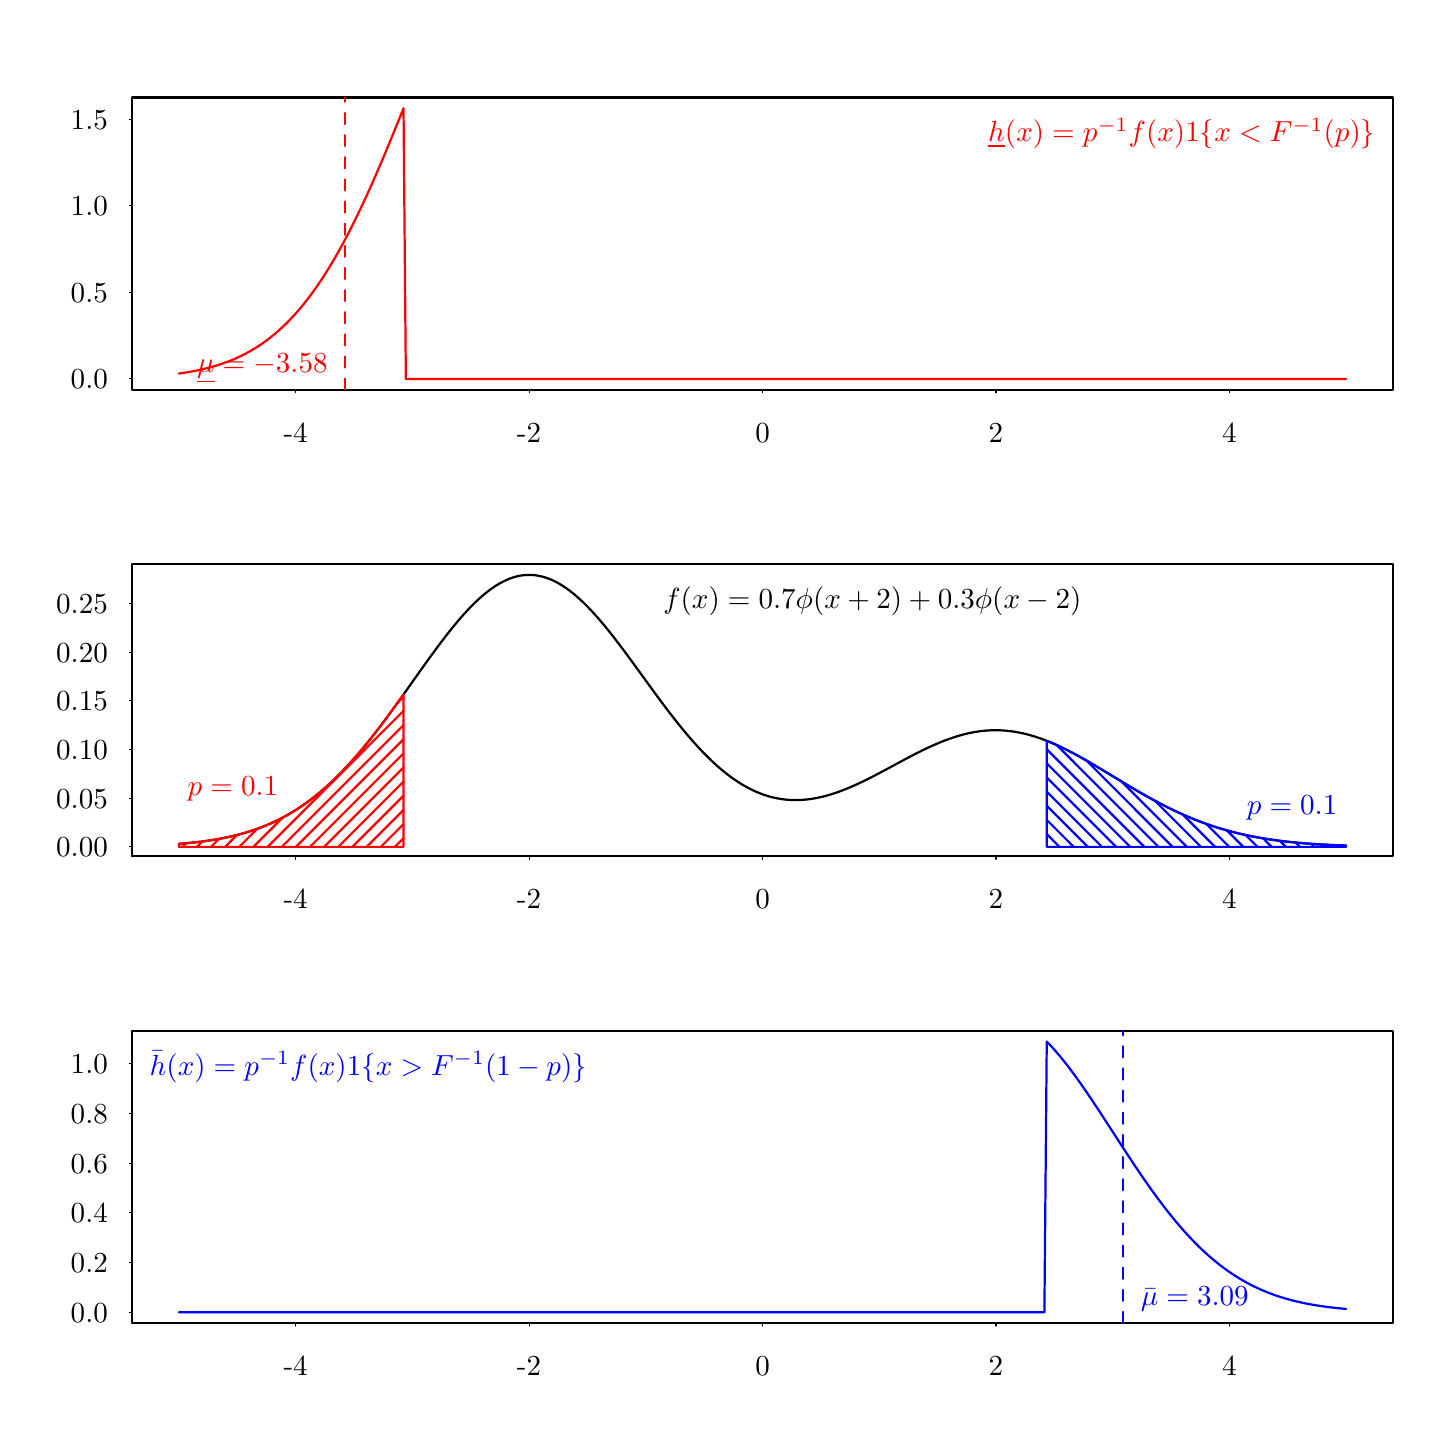
\begin{tikzpicture}[x=1pt,y=1pt]
\definecolor{fillColor}{RGB}{255,255,255}
\path[use as bounding box,fill=fillColor,fill opacity=0.00] (0,0) rectangle (505.89,505.89);
\begin{scope}
\path[clip] ( 37.80,375.06) rectangle (493.29,480.69);
\definecolor{drawColor}{RGB}{255,0,0}

\path[draw=drawColor,line width= 0.8pt,line join=round,line cap=round] ( 54.67,380.91) --
	( 55.52,381.03) --
	( 56.36,381.16) --
	( 57.21,381.29) --
	( 58.05,381.43) --
	( 58.90,381.58) --
	( 59.74,381.73) --
	( 60.59,381.90) --
	( 61.43,382.07) --
	( 62.28,382.25) --
	( 63.12,382.44) --
	( 63.97,382.64) --
	( 64.81,382.85) --
	( 65.66,383.07) --
	( 66.50,383.30) --
	( 67.35,383.54) --
	( 68.19,383.79) --
	( 69.04,384.06) --
	( 69.88,384.33) --
	( 70.73,384.62) --
	( 71.57,384.93) --
	( 72.42,385.24) --
	( 73.26,385.57) --
	( 74.11,385.92) --
	( 74.95,386.28) --
	( 75.80,386.66) --
	( 76.64,387.05) --
	( 77.49,387.46) --
	( 78.34,387.89) --
	( 79.18,388.33) --
	( 80.03,388.80) --
	( 80.87,389.28) --
	( 81.72,389.78) --
	( 82.56,390.30) --
	( 83.41,390.84) --
	( 84.25,391.40) --
	( 85.10,391.99) --
	( 85.94,392.59) --
	( 86.79,393.22) --
	( 87.63,393.87) --
	( 88.48,394.55) --
	( 89.32,395.24) --
	( 90.17,395.97) --
	( 91.01,396.71) --
	( 91.86,397.49) --
	( 92.70,398.29) --
	( 93.55,399.11) --
	( 94.39,399.96) --
	( 95.24,400.84) --
	( 96.08,401.75) --
	( 96.93,402.69) --
	( 97.77,403.65) --
	( 98.62,404.64) --
	( 99.47,405.66) --
	(100.31,406.72) --
	(101.16,407.80) --
	(102.00,408.91) --
	(102.85,410.05) --
	(103.69,411.22) --
	(104.54,412.42) --
	(105.38,413.66) --
	(106.23,414.92) --
	(107.07,416.22) --
	(107.92,417.55) --
	(108.76,418.91) --
	(109.61,420.30) --
	(110.45,421.72) --
	(111.30,423.17) --
	(112.14,424.65) --
	(112.99,426.17) --
	(113.83,427.71) --
	(114.68,429.29) --
	(115.52,430.89) --
	(116.37,432.53) --
	(117.21,434.19) --
	(118.06,435.89) --
	(118.90,437.61) --
	(119.75,439.36) --
	(120.59,441.13) --
	(121.44,442.94) --
	(122.29,444.77) --
	(123.13,446.62) --
	(123.98,448.50) --
	(124.82,450.40) --
	(125.67,452.32) --
	(126.51,454.27) --
	(127.36,456.24) --
	(128.20,458.22) --
	(129.05,460.23) --
	(129.89,462.25) --
	(130.74,464.29) --
	(131.58,466.34) --
	(132.43,468.41) --
	(133.27,470.48) --
	(134.12,472.57) --
	(134.96,474.67) --
	(135.81,476.78) --
	(136.65,378.97) --
	(137.50,378.97) --
	(138.34,378.97) --
	(139.19,378.97) --
	(140.03,378.97) --
	(140.88,378.97) --
	(141.72,378.97) --
	(142.57,378.97) --
	(143.41,378.97) --
	(144.26,378.97) --
	(145.11,378.97) --
	(145.95,378.97) --
	(146.80,378.97) --
	(147.64,378.97) --
	(148.49,378.97) --
	(149.33,378.97) --
	(150.18,378.97) --
	(151.02,378.97) --
	(151.87,378.97) --
	(152.71,378.97) --
	(153.56,378.97) --
	(154.40,378.97) --
	(155.25,378.97) --
	(156.09,378.97) --
	(156.94,378.97) --
	(157.78,378.97) --
	(158.63,378.97) --
	(159.47,378.97) --
	(160.32,378.97) --
	(161.16,378.97) --
	(162.01,378.97) --
	(162.85,378.97) --
	(163.70,378.97) --
	(164.54,378.97) --
	(165.39,378.97) --
	(166.24,378.97) --
	(167.08,378.97) --
	(167.93,378.97) --
	(168.77,378.97) --
	(169.62,378.97) --
	(170.46,378.97) --
	(171.31,378.97) --
	(172.15,378.97) --
	(173.00,378.97) --
	(173.84,378.97) --
	(174.69,378.97) --
	(175.53,378.97) --
	(176.38,378.97) --
	(177.22,378.97) --
	(178.07,378.97) --
	(178.91,378.97) --
	(179.76,378.97) --
	(180.60,378.97) --
	(181.45,378.97) --
	(182.29,378.97) --
	(183.14,378.97) --
	(183.98,378.97) --
	(184.83,378.97) --
	(185.67,378.97) --
	(186.52,378.97) --
	(187.36,378.97) --
	(188.21,378.97) --
	(189.06,378.97) --
	(189.90,378.97) --
	(190.75,378.97) --
	(191.59,378.97) --
	(192.44,378.97) --
	(193.28,378.97) --
	(194.13,378.97) --
	(194.97,378.97) --
	(195.82,378.97) --
	(196.66,378.97) --
	(197.51,378.97) --
	(198.35,378.97) --
	(199.20,378.97) --
	(200.04,378.97) --
	(200.89,378.97) --
	(201.73,378.97) --
	(202.58,378.97) --
	(203.42,378.97) --
	(204.27,378.97) --
	(205.11,378.97) --
	(205.96,378.97) --
	(206.80,378.97) --
	(207.65,378.97) --
	(208.49,378.97) --
	(209.34,378.97) --
	(210.19,378.97) --
	(211.03,378.97) --
	(211.88,378.97) --
	(212.72,378.97) --
	(213.57,378.97) --
	(214.41,378.97) --
	(215.26,378.97) --
	(216.10,378.97) --
	(216.95,378.97) --
	(217.79,378.97) --
	(218.64,378.97) --
	(219.48,378.97) --
	(220.33,378.97) --
	(221.17,378.97) --
	(222.02,378.97) --
	(222.86,378.97) --
	(223.71,378.97) --
	(224.55,378.97) --
	(225.40,378.97) --
	(226.24,378.97) --
	(227.09,378.97) --
	(227.93,378.97) --
	(228.78,378.97) --
	(229.62,378.97) --
	(230.47,378.97) --
	(231.31,378.97) --
	(232.16,378.97) --
	(233.01,378.97) --
	(233.85,378.97) --
	(234.70,378.97) --
	(235.54,378.97) --
	(236.39,378.97) --
	(237.23,378.97) --
	(238.08,378.97) --
	(238.92,378.97) --
	(239.77,378.97) --
	(240.61,378.97) --
	(241.46,378.97) --
	(242.30,378.97) --
	(243.15,378.97) --
	(243.99,378.97) --
	(244.84,378.97) --
	(245.68,378.97) --
	(246.53,378.97) --
	(247.37,378.97) --
	(248.22,378.97) --
	(249.06,378.97) --
	(249.91,378.97) --
	(250.75,378.97) --
	(251.60,378.97) --
	(252.44,378.97) --
	(253.29,378.97) --
	(254.13,378.97) --
	(254.98,378.97) --
	(255.83,378.97) --
	(256.67,378.97) --
	(257.52,378.97) --
	(258.36,378.97) --
	(259.21,378.97) --
	(260.05,378.97) --
	(260.90,378.97) --
	(261.74,378.97) --
	(262.59,378.97) --
	(263.43,378.97) --
	(264.28,378.97) --
	(265.12,378.97) --
	(265.97,378.97) --
	(266.81,378.97) --
	(267.66,378.97) --
	(268.50,378.97) --
	(269.35,378.97) --
	(270.19,378.97) --
	(271.04,378.97) --
	(271.88,378.97) --
	(272.73,378.97) --
	(273.57,378.97) --
	(274.42,378.97) --
	(275.26,378.97) --
	(276.11,378.97) --
	(276.96,378.97) --
	(277.80,378.97) --
	(278.65,378.97) --
	(279.49,378.97) --
	(280.34,378.97) --
	(281.18,378.97) --
	(282.03,378.97) --
	(282.87,378.97) --
	(283.72,378.97) --
	(284.56,378.97) --
	(285.41,378.97) --
	(286.25,378.97) --
	(287.10,378.97) --
	(287.94,378.97) --
	(288.79,378.97) --
	(289.63,378.97) --
	(290.48,378.97) --
	(291.32,378.97) --
	(292.17,378.97) --
	(293.01,378.97) --
	(293.86,378.97) --
	(294.70,378.97) --
	(295.55,378.97) --
	(296.39,378.97) --
	(297.24,378.97) --
	(298.08,378.97) --
	(298.93,378.97) --
	(299.78,378.97) --
	(300.62,378.97) --
	(301.47,378.97) --
	(302.31,378.97) --
	(303.16,378.97) --
	(304.00,378.97) --
	(304.85,378.97) --
	(305.69,378.97) --
	(306.54,378.97) --
	(307.38,378.97) --
	(308.23,378.97) --
	(309.07,378.97) --
	(309.92,378.97) --
	(310.76,378.97) --
	(311.61,378.97) --
	(312.45,378.97) --
	(313.30,378.97) --
	(314.14,378.97) --
	(314.99,378.97) --
	(315.83,378.97) --
	(316.68,378.97) --
	(317.52,378.97) --
	(318.37,378.97) --
	(319.21,378.97) --
	(320.06,378.97) --
	(320.90,378.97) --
	(321.75,378.97) --
	(322.60,378.97) --
	(323.44,378.97) --
	(324.29,378.97) --
	(325.13,378.97) --
	(325.98,378.97) --
	(326.82,378.97) --
	(327.67,378.97) --
	(328.51,378.97) --
	(329.36,378.97) --
	(330.20,378.97) --
	(331.05,378.97) --
	(331.89,378.97) --
	(332.74,378.97) --
	(333.58,378.97) --
	(334.43,378.97) --
	(335.27,378.97) --
	(336.12,378.97) --
	(336.96,378.97) --
	(337.81,378.97) --
	(338.65,378.97) --
	(339.50,378.97) --
	(340.34,378.97) --
	(341.19,378.97) --
	(342.03,378.97) --
	(342.88,378.97) --
	(343.73,378.97) --
	(344.57,378.97) --
	(345.42,378.97) --
	(346.26,378.97) --
	(347.11,378.97) --
	(347.95,378.97) --
	(348.80,378.97) --
	(349.64,378.97) --
	(350.49,378.97) --
	(351.33,378.97) --
	(352.18,378.97) --
	(353.02,378.97) --
	(353.87,378.97) --
	(354.71,378.97) --
	(355.56,378.97) --
	(356.40,378.97) --
	(357.25,378.97) --
	(358.09,378.97) --
	(358.94,378.97) --
	(359.78,378.97) --
	(360.63,378.97) --
	(361.47,378.97) --
	(362.32,378.97) --
	(363.16,378.97) --
	(364.01,378.97) --
	(364.85,378.97) --
	(365.70,378.97) --
	(366.55,378.97) --
	(367.39,378.97) --
	(368.24,378.97) --
	(369.08,378.97) --
	(369.93,378.97) --
	(370.77,378.97) --
	(371.62,378.97) --
	(372.46,378.97) --
	(373.31,378.97) --
	(374.15,378.97) --
	(375.00,378.97) --
	(375.84,378.97) --
	(376.69,378.97) --
	(377.53,378.97) --
	(378.38,378.97) --
	(379.22,378.97) --
	(380.07,378.97) --
	(380.91,378.97) --
	(381.76,378.97) --
	(382.60,378.97) --
	(383.45,378.97) --
	(384.29,378.97) --
	(385.14,378.97) --
	(385.98,378.97) --
	(386.83,378.97) --
	(387.68,378.97) --
	(388.52,378.97) --
	(389.37,378.97) --
	(390.21,378.97) --
	(391.06,378.97) --
	(391.90,378.97) --
	(392.75,378.97) --
	(393.59,378.97) --
	(394.44,378.97) --
	(395.28,378.97) --
	(396.13,378.97) --
	(396.97,378.97) --
	(397.82,378.97) --
	(398.66,378.97) --
	(399.51,378.97) --
	(400.35,378.97) --
	(401.20,378.97) --
	(402.04,378.97) --
	(402.89,378.97) --
	(403.73,378.97) --
	(404.58,378.97) --
	(405.42,378.97) --
	(406.27,378.97) --
	(407.11,378.97) --
	(407.96,378.97) --
	(408.80,378.97) --
	(409.65,378.97) --
	(410.50,378.97) --
	(411.34,378.97) --
	(412.19,378.97) --
	(413.03,378.97) --
	(413.88,378.97) --
	(414.72,378.97) --
	(415.57,378.97) --
	(416.41,378.97) --
	(417.26,378.97) --
	(418.10,378.97) --
	(418.95,378.97) --
	(419.79,378.97) --
	(420.64,378.97) --
	(421.48,378.97) --
	(422.33,378.97) --
	(423.17,378.97) --
	(424.02,378.97) --
	(424.86,378.97) --
	(425.71,378.97) --
	(426.55,378.97) --
	(427.40,378.97) --
	(428.24,378.97) --
	(429.09,378.97) --
	(429.93,378.97) --
	(430.78,378.97) --
	(431.62,378.97) --
	(432.47,378.97) --
	(433.32,378.97) --
	(434.16,378.97) --
	(435.01,378.97) --
	(435.85,378.97) --
	(436.70,378.97) --
	(437.54,378.97) --
	(438.39,378.97) --
	(439.23,378.97) --
	(440.08,378.97) --
	(440.92,378.97) --
	(441.77,378.97) --
	(442.61,378.97) --
	(443.46,378.97) --
	(444.30,378.97) --
	(445.15,378.97) --
	(445.99,378.97) --
	(446.84,378.97) --
	(447.68,378.97) --
	(448.53,378.97) --
	(449.37,378.97) --
	(450.22,378.97) --
	(451.06,378.97) --
	(451.91,378.97) --
	(452.75,378.97) --
	(453.60,378.97) --
	(454.45,378.97) --
	(455.29,378.97) --
	(456.14,378.97) --
	(456.98,378.97) --
	(457.83,378.97) --
	(458.67,378.97) --
	(459.52,378.97) --
	(460.36,378.97) --
	(461.21,378.97) --
	(462.05,378.97) --
	(462.90,378.97) --
	(463.74,378.97) --
	(464.59,378.97) --
	(465.43,378.97) --
	(466.28,378.97) --
	(467.12,378.97) --
	(467.97,378.97) --
	(468.81,378.97) --
	(469.66,378.97) --
	(470.50,378.97) --
	(471.35,378.97) --
	(472.19,378.97) --
	(473.04,378.97) --
	(473.88,378.97) --
	(474.73,378.97) --
	(475.57,378.97) --
	(476.42,378.97);
\end{scope}
\begin{scope}
\path[clip] (  0.00,  0.00) rectangle (505.89,505.89);
\definecolor{drawColor}{RGB}{0,0,0}

\path[draw=drawColor,line width= 0.4pt,line join=round,line cap=round] ( 96.84,375.06) -- (434.25,375.06);

\path[draw=drawColor,line width= 0.4pt,line join=round,line cap=round] ( 96.84,375.06) -- ( 96.84,374.00);

\path[draw=drawColor,line width= 0.4pt,line join=round,line cap=round] (181.19,375.06) -- (181.19,374.00);

\path[draw=drawColor,line width= 0.4pt,line join=round,line cap=round] (265.54,375.06) -- (265.54,374.00);

\path[draw=drawColor,line width= 0.4pt,line join=round,line cap=round] (349.89,375.06) -- (349.89,374.00);

\path[draw=drawColor,line width= 0.4pt,line join=round,line cap=round] (434.25,375.06) -- (434.25,374.00);

\node[text=drawColor,anchor=base,inner sep=0pt, outer sep=0pt, scale=  1.05] at ( 96.84,356.16) {-4};

\node[text=drawColor,anchor=base,inner sep=0pt, outer sep=0pt, scale=  1.05] at (181.19,356.16) {-2};

\node[text=drawColor,anchor=base,inner sep=0pt, outer sep=0pt, scale=  1.05] at (265.54,356.16) {0};

\node[text=drawColor,anchor=base,inner sep=0pt, outer sep=0pt, scale=  1.05] at (349.89,356.16) {2};

\node[text=drawColor,anchor=base,inner sep=0pt, outer sep=0pt, scale=  1.05] at (434.25,356.16) {4};

\path[draw=drawColor,line width= 0.4pt,line join=round,line cap=round] ( 37.80,378.97) -- ( 37.80,472.71);

\path[draw=drawColor,line width= 0.4pt,line join=round,line cap=round] ( 37.80,378.97) -- ( 36.74,378.97);

\path[draw=drawColor,line width= 0.4pt,line join=round,line cap=round] ( 37.80,410.22) -- ( 36.74,410.22);

\path[draw=drawColor,line width= 0.4pt,line join=round,line cap=round] ( 37.80,441.47) -- ( 36.74,441.47);

\path[draw=drawColor,line width= 0.4pt,line join=round,line cap=round] ( 37.80,472.71) -- ( 36.74,472.71);

\node[text=drawColor,anchor=base east,inner sep=0pt, outer sep=0pt, scale=  1.05] at ( 28.98,375.36) {0.0};

\node[text=drawColor,anchor=base east,inner sep=0pt, outer sep=0pt, scale=  1.05] at ( 28.98,406.60) {0.5};

\node[text=drawColor,anchor=base east,inner sep=0pt, outer sep=0pt, scale=  1.05] at ( 28.98,437.85) {1.0};

\node[text=drawColor,anchor=base east,inner sep=0pt, outer sep=0pt, scale=  1.05] at ( 28.98,469.10) {1.5};

\path[draw=drawColor,line width= 0.8pt,line join=round,line cap=round] ( 37.80,375.06) --
	(493.29,375.06) --
	(493.29,480.69) --
	( 37.80,480.69) --
	( 37.80,375.06);
\end{scope}
\begin{scope}
\path[clip] ( 37.80,375.06) rectangle (493.29,480.69);
\definecolor{drawColor}{RGB}{255,0,0}

\node[text=drawColor,anchor=base east,inner sep=0pt, outer sep=0pt, scale=  1.05] at (486.99,464.59) {$\underline{h}(x) = p^{-1}f(x) 1\{x < F^{-1}(p)\}$};

\path[draw=drawColor,line width= 0.8pt,dash pattern=on 4pt off 4pt ,line join=round,line cap=round] (114.67,375.06) -- (114.67,480.69);

\node[text=drawColor,anchor=base east,inner sep=0pt, outer sep=0pt, scale=  1.05] at (108.37,381.45) {$\underline{\mu} = -3.58$};
\end{scope}
\begin{scope}
\path[clip] ( 37.80,206.43) rectangle (493.29,312.06);
\definecolor{drawColor}{RGB}{0,0,0}

\path[draw=drawColor,line width= 0.8pt,line join=round,line cap=round] ( 54.67,210.97) --
	( 55.52,211.03) --
	( 56.36,211.10) --
	( 57.21,211.18) --
	( 58.05,211.26) --
	( 58.90,211.34) --
	( 59.74,211.43) --
	( 60.59,211.52) --
	( 61.43,211.62) --
	( 62.28,211.72) --
	( 63.12,211.83) --
	( 63.97,211.94) --
	( 64.81,212.06) --
	( 65.66,212.18) --
	( 66.50,212.31) --
	( 67.35,212.45) --
	( 68.19,212.59) --
	( 69.04,212.74) --
	( 69.88,212.89) --
	( 70.73,213.06) --
	( 71.57,213.23) --
	( 72.42,213.41) --
	( 73.26,213.59) --
	( 74.11,213.79) --
	( 74.95,213.99) --
	( 75.80,214.20) --
	( 76.64,214.42) --
	( 77.49,214.65) --
	( 78.34,214.90) --
	( 79.18,215.15) --
	( 80.03,215.41) --
	( 80.87,215.68) --
	( 81.72,215.96) --
	( 82.56,216.25) --
	( 83.41,216.56) --
	( 84.25,216.87) --
	( 85.10,217.20) --
	( 85.94,217.54) --
	( 86.79,217.90) --
	( 87.63,218.26) --
	( 88.48,218.64) --
	( 89.32,219.04) --
	( 90.17,219.44) --
	( 91.01,219.86) --
	( 91.86,220.30) --
	( 92.70,220.75) --
	( 93.55,221.21) --
	( 94.39,221.69) --
	( 95.24,222.19) --
	( 96.08,222.70) --
	( 96.93,223.23) --
	( 97.77,223.77) --
	( 98.62,224.33) --
	( 99.47,224.90) --
	(100.31,225.49) --
	(101.16,226.10) --
	(102.00,226.73) --
	(102.85,227.37) --
	(103.69,228.03) --
	(104.54,228.71) --
	(105.38,229.40) --
	(106.23,230.12) --
	(107.07,230.85) --
	(107.92,231.59) --
	(108.76,232.36) --
	(109.61,233.14) --
	(110.45,233.94) --
	(111.30,234.76) --
	(112.14,235.59) --
	(112.99,236.45) --
	(113.83,237.32) --
	(114.68,238.20) --
	(115.52,239.11) --
	(116.37,240.03) --
	(117.21,240.97) --
	(118.06,241.92) --
	(118.90,242.89) --
	(119.75,243.87) --
	(120.59,244.87) --
	(121.44,245.89) --
	(122.29,246.92) --
	(123.13,247.96) --
	(123.98,249.02) --
	(124.82,250.09) --
	(125.67,251.17) --
	(126.51,252.27) --
	(127.36,253.38) --
	(128.20,254.50) --
	(129.05,255.62) --
	(129.89,256.76) --
	(130.74,257.91) --
	(131.58,259.07) --
	(132.43,260.23) --
	(133.27,261.40) --
	(134.12,262.58) --
	(134.96,263.76) --
	(135.81,264.94) --
	(136.65,266.13) --
	(137.50,267.32) --
	(138.34,268.52) --
	(139.19,269.71) --
	(140.03,270.91) --
	(140.88,272.10) --
	(141.72,273.29) --
	(142.57,274.48) --
	(143.41,275.66) --
	(144.26,276.84) --
	(145.11,278.01) --
	(145.95,279.18) --
	(146.80,280.33) --
	(147.64,281.48) --
	(148.49,282.61) --
	(149.33,283.74) --
	(150.18,284.85) --
	(151.02,285.95) --
	(151.87,287.03) --
	(152.71,288.10) --
	(153.56,289.15) --
	(154.40,290.18) --
	(155.25,291.19) --
	(156.09,292.19) --
	(156.94,293.16) --
	(157.78,294.11) --
	(158.63,295.03) --
	(159.47,295.93) --
	(160.32,296.81) --
	(161.16,297.66) --
	(162.01,298.48) --
	(162.85,299.27) --
	(163.70,300.04) --
	(164.54,300.77) --
	(165.39,301.47) --
	(166.24,302.15) --
	(167.08,302.79) --
	(167.93,303.39) --
	(168.77,303.97) --
	(169.62,304.51) --
	(170.46,305.01) --
	(171.31,305.48) --
	(172.15,305.91) --
	(173.00,306.30) --
	(173.84,306.66) --
	(174.69,306.98) --
	(175.53,307.26) --
	(176.38,307.50) --
	(177.22,307.71) --
	(178.07,307.88) --
	(178.91,308.00) --
	(179.76,308.09) --
	(180.60,308.14) --
	(181.45,308.15) --
	(182.29,308.12) --
	(183.14,308.05) --
	(183.98,307.94) --
	(184.83,307.79) --
	(185.67,307.60) --
	(186.52,307.38) --
	(187.36,307.11) --
	(188.21,306.81) --
	(189.06,306.47) --
	(189.90,306.10) --
	(190.75,305.68) --
	(191.59,305.23) --
	(192.44,304.75) --
	(193.28,304.22) --
	(194.13,303.67) --
	(194.97,303.08) --
	(195.82,302.46) --
	(196.66,301.80) --
	(197.51,301.12) --
	(198.35,300.40) --
	(199.20,299.65) --
	(200.04,298.87) --
	(200.89,298.07) --
	(201.73,297.24) --
	(202.58,296.38) --
	(203.42,295.49) --
	(204.27,294.59) --
	(205.11,293.65) --
	(205.96,292.70) --
	(206.80,291.73) --
	(207.65,290.73) --
	(208.49,289.72) --
	(209.34,288.68) --
	(210.19,287.63) --
	(211.03,286.57) --
	(211.88,285.49) --
	(212.72,284.40) --
	(213.57,283.29) --
	(214.41,282.18) --
	(215.26,281.05) --
	(216.10,279.91) --
	(216.95,278.77) --
	(217.79,277.62) --
	(218.64,276.46) --
	(219.48,275.30) --
	(220.33,274.14) --
	(221.17,272.97) --
	(222.02,271.81) --
	(222.86,270.64) --
	(223.71,269.47) --
	(224.55,268.31) --
	(225.40,267.15) --
	(226.24,265.99) --
	(227.09,264.84) --
	(227.93,263.69) --
	(228.78,262.55) --
	(229.62,261.42) --
	(230.47,260.29) --
	(231.31,259.18) --
	(232.16,258.08) --
	(233.01,256.98) --
	(233.85,255.90) --
	(234.70,254.83) --
	(235.54,253.78) --
	(236.39,252.74) --
	(237.23,251.71) --
	(238.08,250.70) --
	(238.92,249.71) --
	(239.77,248.73) --
	(240.61,247.77) --
	(241.46,246.82) --
	(242.30,245.90) --
	(243.15,244.99) --
	(243.99,244.10) --
	(244.84,243.24) --
	(245.68,242.39) --
	(246.53,241.56) --
	(247.37,240.76) --
	(248.22,239.97) --
	(249.06,239.21) --
	(249.91,238.47) --
	(250.75,237.75) --
	(251.60,237.05) --
	(252.44,236.38) --
	(253.29,235.73) --
	(254.13,235.10) --
	(254.98,234.49) --
	(255.83,233.91) --
	(256.67,233.35) --
	(257.52,232.81) --
	(258.36,232.30) --
	(259.21,231.81) --
	(260.05,231.34) --
	(260.90,230.90) --
	(261.74,230.48) --
	(262.59,230.08) --
	(263.43,229.70) --
	(264.28,229.35) --
	(265.12,229.03) --
	(265.97,228.72) --
	(266.81,228.44) --
	(267.66,228.18) --
	(268.50,227.94) --
	(269.35,227.73) --
	(270.19,227.54) --
	(271.04,227.37) --
	(271.88,227.22) --
	(272.73,227.09) --
	(273.57,226.99) --
	(274.42,226.90) --
	(275.26,226.84) --
	(276.11,226.80) --
	(276.96,226.78) --
	(277.80,226.77) --
	(278.65,226.79) --
	(279.49,226.83) --
	(280.34,226.88) --
	(281.18,226.96) --
	(282.03,227.05) --
	(282.87,227.16) --
	(283.72,227.29) --
	(284.56,227.44) --
	(285.41,227.60) --
	(286.25,227.78) --
	(287.10,227.97) --
	(287.94,228.18) --
	(288.79,228.41) --
	(289.63,228.65) --
	(290.48,228.91) --
	(291.32,229.18) --
	(292.17,229.46) --
	(293.01,229.76) --
	(293.86,230.07) --
	(294.70,230.39) --
	(295.55,230.72) --
	(296.39,231.07) --
	(297.24,231.42) --
	(298.08,231.79) --
	(298.93,232.16) --
	(299.78,232.55) --
	(300.62,232.94) --
	(301.47,233.34) --
	(302.31,233.75) --
	(303.16,234.16) --
	(304.00,234.59) --
	(304.85,235.01) --
	(305.69,235.45) --
	(306.54,235.89) --
	(307.38,236.33) --
	(308.23,236.78) --
	(309.07,237.23) --
	(309.92,237.68) --
	(310.76,238.13) --
	(311.61,238.59) --
	(312.45,239.05) --
	(313.30,239.50) --
	(314.14,239.96) --
	(314.99,240.41) --
	(315.83,240.87) --
	(316.68,241.32) --
	(317.52,241.77) --
	(318.37,242.22) --
	(319.21,242.66) --
	(320.06,243.10) --
	(320.90,243.53) --
	(321.75,243.96) --
	(322.60,244.38) --
	(323.44,244.80) --
	(324.29,245.21) --
	(325.13,245.61) --
	(325.98,246.00) --
	(326.82,246.39) --
	(327.67,246.76) --
	(328.51,247.13) --
	(329.36,247.48) --
	(330.20,247.83) --
	(331.05,248.16) --
	(331.89,248.49) --
	(332.74,248.80) --
	(333.58,249.09) --
	(334.43,249.38) --
	(335.27,249.65) --
	(336.12,249.91) --
	(336.96,250.16) --
	(337.81,250.39) --
	(338.65,250.61) --
	(339.50,250.81) --
	(340.34,251.00) --
	(341.19,251.17) --
	(342.03,251.33) --
	(342.88,251.47) --
	(343.73,251.60) --
	(344.57,251.71) --
	(345.42,251.80) --
	(346.26,251.88) --
	(347.11,251.94) --
	(347.95,251.98) --
	(348.80,252.01) --
	(349.64,252.02) --
	(350.49,252.01) --
	(351.33,251.99) --
	(352.18,251.95) --
	(353.02,251.89) --
	(353.87,251.82) --
	(354.71,251.73) --
	(355.56,251.63) --
	(356.40,251.51) --
	(357.25,251.37) --
	(358.09,251.21) --
	(358.94,251.04) --
	(359.78,250.86) --
	(360.63,250.66) --
	(361.47,250.44) --
	(362.32,250.21) --
	(363.16,249.96) --
	(364.01,249.70) --
	(364.85,249.43) --
	(365.70,249.14) --
	(366.55,248.84) --
	(367.39,248.52) --
	(368.24,248.19) --
	(369.08,247.85) --
	(369.93,247.50) --
	(370.77,247.13) --
	(371.62,246.76) --
	(372.46,246.37) --
	(373.31,245.98) --
	(374.15,245.57) --
	(375.00,245.15) --
	(375.84,244.73) --
	(376.69,244.29) --
	(377.53,243.85) --
	(378.38,243.40) --
	(379.22,242.94) --
	(380.07,242.48) --
	(380.91,242.01) --
	(381.76,241.53) --
	(382.60,241.05) --
	(383.45,240.56) --
	(384.29,240.07) --
	(385.14,239.58) --
	(385.98,239.08) --
	(386.83,238.57) --
	(387.68,238.07) --
	(388.52,237.56) --
	(389.37,237.05) --
	(390.21,236.54) --
	(391.06,236.03) --
	(391.90,235.52) --
	(392.75,235.01) --
	(393.59,234.50) --
	(394.44,233.98) --
	(395.28,233.48) --
	(396.13,232.97) --
	(396.97,232.46) --
	(397.82,231.96) --
	(398.66,231.46) --
	(399.51,230.96) --
	(400.35,230.46) --
	(401.20,229.97) --
	(402.04,229.48) --
	(402.89,229.00) --
	(403.73,228.52) --
	(404.58,228.04) --
	(405.42,227.57) --
	(406.27,227.11) --
	(407.11,226.65) --
	(407.96,226.20) --
	(408.80,225.75) --
	(409.65,225.31) --
	(410.50,224.87) --
	(411.34,224.45) --
	(412.19,224.02) --
	(413.03,223.61) --
	(413.88,223.20) --
	(414.72,222.80) --
	(415.57,222.40) --
	(416.41,222.02) --
	(417.26,221.64) --
	(418.10,221.26) --
	(418.95,220.90) --
	(419.79,220.54) --
	(420.64,220.19) --
	(421.48,219.85) --
	(422.33,219.51) --
	(423.17,219.18) --
	(424.02,218.86) --
	(424.86,218.55) --
	(425.71,218.24) --
	(426.55,217.95) --
	(427.40,217.66) --
	(428.24,217.37) --
	(429.09,217.10) --
	(429.93,216.83) --
	(430.78,216.57) --
	(431.62,216.32) --
	(432.47,216.07) --
	(433.32,215.83) --
	(434.16,215.60) --
	(435.01,215.37) --
	(435.85,215.15) --
	(436.70,214.94) --
	(437.54,214.73) --
	(438.39,214.53) --
	(439.23,214.34) --
	(440.08,214.16) --
	(440.92,213.98) --
	(441.77,213.80) --
	(442.61,213.63) --
	(443.46,213.47) --
	(444.30,213.31) --
	(445.15,213.16) --
	(445.99,213.02) --
	(446.84,212.87) --
	(447.68,212.74) --
	(448.53,212.61) --
	(449.37,212.48) --
	(450.22,212.36) --
	(451.06,212.25) --
	(451.91,212.13) --
	(452.75,212.03) --
	(453.60,211.92) --
	(454.45,211.82) --
	(455.29,211.73) --
	(456.14,211.64) --
	(456.98,211.55) --
	(457.83,211.47) --
	(458.67,211.39) --
	(459.52,211.31) --
	(460.36,211.24) --
	(461.21,211.17) --
	(462.05,211.10) --
	(462.90,211.04) --
	(463.74,210.98) --
	(464.59,210.92) --
	(465.43,210.86) --
	(466.28,210.81) --
	(467.12,210.76) --
	(467.97,210.71) --
	(468.81,210.67) --
	(469.66,210.62) --
	(470.50,210.58) --
	(471.35,210.54) --
	(472.19,210.50) --
	(473.04,210.47) --
	(473.88,210.43) --
	(474.73,210.40) --
	(475.57,210.37) --
	(476.42,210.34);
\end{scope}
\begin{scope}
\path[clip] (  0.00,  0.00) rectangle (505.89,505.89);
\definecolor{drawColor}{RGB}{0,0,0}

\path[draw=drawColor,line width= 0.4pt,line join=round,line cap=round] ( 96.84,206.43) -- (434.25,206.43);

\path[draw=drawColor,line width= 0.4pt,line join=round,line cap=round] ( 96.84,206.43) -- ( 96.84,205.37);

\path[draw=drawColor,line width= 0.4pt,line join=round,line cap=round] (181.19,206.43) -- (181.19,205.37);

\path[draw=drawColor,line width= 0.4pt,line join=round,line cap=round] (265.54,206.43) -- (265.54,205.37);

\path[draw=drawColor,line width= 0.4pt,line join=round,line cap=round] (349.89,206.43) -- (349.89,205.37);

\path[draw=drawColor,line width= 0.4pt,line join=round,line cap=round] (434.25,206.43) -- (434.25,205.37);

\node[text=drawColor,anchor=base,inner sep=0pt, outer sep=0pt, scale=  1.05] at ( 96.84,187.53) {-4};

\node[text=drawColor,anchor=base,inner sep=0pt, outer sep=0pt, scale=  1.05] at (181.19,187.53) {-2};

\node[text=drawColor,anchor=base,inner sep=0pt, outer sep=0pt, scale=  1.05] at (265.54,187.53) {0};

\node[text=drawColor,anchor=base,inner sep=0pt, outer sep=0pt, scale=  1.05] at (349.89,187.53) {2};

\node[text=drawColor,anchor=base,inner sep=0pt, outer sep=0pt, scale=  1.05] at (434.25,187.53) {4};

\path[draw=drawColor,line width= 0.4pt,line join=round,line cap=round] ( 37.80,209.87) -- ( 37.80,297.84);

\path[draw=drawColor,line width= 0.4pt,line join=round,line cap=round] ( 37.80,209.87) -- ( 36.74,209.87);

\path[draw=drawColor,line width= 0.4pt,line join=round,line cap=round] ( 37.80,227.47) -- ( 36.74,227.47);

\path[draw=drawColor,line width= 0.4pt,line join=round,line cap=round] ( 37.80,245.06) -- ( 36.74,245.06);

\path[draw=drawColor,line width= 0.4pt,line join=round,line cap=round] ( 37.80,262.65) -- ( 36.74,262.65);

\path[draw=drawColor,line width= 0.4pt,line join=round,line cap=round] ( 37.80,280.25) -- ( 36.74,280.25);

\path[draw=drawColor,line width= 0.4pt,line join=round,line cap=round] ( 37.80,297.84) -- ( 36.74,297.84);

\node[text=drawColor,anchor=base east,inner sep=0pt, outer sep=0pt, scale=  1.05] at ( 28.98,206.26) {0.00};

\node[text=drawColor,anchor=base east,inner sep=0pt, outer sep=0pt, scale=  1.05] at ( 28.98,223.85) {0.05};

\node[text=drawColor,anchor=base east,inner sep=0pt, outer sep=0pt, scale=  1.05] at ( 28.98,241.44) {0.10};

\node[text=drawColor,anchor=base east,inner sep=0pt, outer sep=0pt, scale=  1.05] at ( 28.98,259.04) {0.15};

\node[text=drawColor,anchor=base east,inner sep=0pt, outer sep=0pt, scale=  1.05] at ( 28.98,276.63) {0.20};

\node[text=drawColor,anchor=base east,inner sep=0pt, outer sep=0pt, scale=  1.05] at ( 28.98,294.22) {0.25};

\path[draw=drawColor,line width= 0.8pt,line join=round,line cap=round] ( 37.80,206.43) --
	(493.29,206.43) --
	(493.29,312.06) --
	( 37.80,312.06) --
	( 37.80,206.43);
\end{scope}
\begin{scope}
\path[clip] ( 37.80,206.43) rectangle (493.29,312.06);
\definecolor{drawColor}{RGB}{255,0,0}

\path[draw=drawColor,line width= 0.8pt,line join=round,line cap=round] ( 56.02,209.87) -- ( 57.34,211.19);

\path[draw=drawColor,line width= 0.8pt,line join=round,line cap=round] ( 61.13,209.87) -- ( 63.08,211.82);

\path[draw=drawColor,line width= 0.8pt,line join=round,line cap=round] ( 66.24,209.87) -- ( 69.12,212.75);

\path[draw=drawColor,line width= 0.8pt,line join=round,line cap=round] ( 71.36,209.87) -- ( 75.64,214.16);

\path[draw=drawColor,line width= 0.8pt,line join=round,line cap=round] ( 76.47,209.87) -- ( 83.00,216.41);

\path[draw=drawColor,line width= 0.8pt,line join=round,line cap=round] ( 81.58,209.87) -- ( 92.16,220.46);

\path[draw=drawColor,line width= 0.8pt,line join=round,line cap=round] (133.71,262.01) -- (135.81,264.11);

\path[draw=drawColor,line width= 0.8pt,line join=round,line cap=round] ( 86.69,209.87) -- (135.81,259.00);

\path[draw=drawColor,line width= 0.8pt,line join=round,line cap=round] ( 91.80,209.87) -- (135.81,253.89);

\path[draw=drawColor,line width= 0.8pt,line join=round,line cap=round] ( 96.91,209.87) -- (135.81,248.78);

\path[draw=drawColor,line width= 0.8pt,line join=round,line cap=round] (102.02,209.87) -- (135.81,243.67);

\path[draw=drawColor,line width= 0.8pt,line join=round,line cap=round] (107.13,209.87) -- (135.81,238.56);

\path[draw=drawColor,line width= 0.8pt,line join=round,line cap=round] (112.24,209.87) -- (135.81,233.45);

\path[draw=drawColor,line width= 0.8pt,line join=round,line cap=round] (117.35,209.87) -- (135.81,228.34);

\path[draw=drawColor,line width= 0.8pt,line join=round,line cap=round] (122.46,209.87) -- (135.81,223.22);

\path[draw=drawColor,line width= 0.8pt,line join=round,line cap=round] (127.57,209.87) -- (135.81,218.11);

\path[draw=drawColor,line width= 0.8pt,line join=round,line cap=round] (132.68,209.87) -- (135.81,213.00);

\path[draw=drawColor,line width= 0.8pt,line join=round,line cap=round] ( 54.67,209.87) --
	( 55.52,209.87) --
	( 56.36,209.87) --
	( 57.21,209.87) --
	( 58.05,209.87) --
	( 58.90,209.87) --
	( 59.74,209.87) --
	( 60.59,209.87) --
	( 61.43,209.87) --
	( 62.28,209.87) --
	( 63.12,209.87) --
	( 63.97,209.87) --
	( 64.81,209.87) --
	( 65.66,209.87) --
	( 66.50,209.87) --
	( 67.35,209.87) --
	( 68.19,209.87) --
	( 69.04,209.87) --
	( 69.88,209.87) --
	( 70.73,209.87) --
	( 71.57,209.87) --
	( 72.42,209.87) --
	( 73.26,209.87) --
	( 74.11,209.87) --
	( 74.95,209.87) --
	( 75.80,209.87) --
	( 76.64,209.87) --
	( 77.49,209.87) --
	( 78.34,209.87) --
	( 79.18,209.87) --
	( 80.03,209.87) --
	( 80.87,209.87) --
	( 81.72,209.87) --
	( 82.56,209.87) --
	( 83.41,209.87) --
	( 84.25,209.87) --
	( 85.10,209.87) --
	( 85.94,209.87) --
	( 86.79,209.87) --
	( 87.63,209.87) --
	( 88.48,209.87) --
	( 89.32,209.87) --
	( 90.17,209.87) --
	( 91.01,209.87) --
	( 91.86,209.87) --
	( 92.70,209.87) --
	( 93.55,209.87) --
	( 94.39,209.87) --
	( 95.24,209.87) --
	( 96.08,209.87) --
	( 96.93,209.87) --
	( 97.77,209.87) --
	( 98.62,209.87) --
	( 99.47,209.87) --
	(100.31,209.87) --
	(101.16,209.87) --
	(102.00,209.87) --
	(102.85,209.87) --
	(103.69,209.87) --
	(104.54,209.87) --
	(105.38,209.87) --
	(106.23,209.87) --
	(107.07,209.87) --
	(107.92,209.87) --
	(108.76,209.87) --
	(109.61,209.87) --
	(110.45,209.87) --
	(111.30,209.87) --
	(112.14,209.87) --
	(112.99,209.87) --
	(113.83,209.87) --
	(114.68,209.87) --
	(115.52,209.87) --
	(116.37,209.87) --
	(117.21,209.87) --
	(118.06,209.87) --
	(118.90,209.87) --
	(119.75,209.87) --
	(120.59,209.87) --
	(121.44,209.87) --
	(122.29,209.87) --
	(123.13,209.87) --
	(123.98,209.87) --
	(124.82,209.87) --
	(125.67,209.87) --
	(126.51,209.87) --
	(127.36,209.87) --
	(128.20,209.87) --
	(129.05,209.87) --
	(129.89,209.87) --
	(130.74,209.87) --
	(131.58,209.87) --
	(132.43,209.87) --
	(133.27,209.87) --
	(134.12,209.87) --
	(134.96,209.87) --
	(135.81,209.87) --
	(135.81,264.94) --
	(134.96,263.76) --
	(134.12,262.58) --
	(133.27,261.40) --
	(132.43,260.23) --
	(131.58,259.07) --
	(130.74,257.91) --
	(129.89,256.76) --
	(129.05,255.62) --
	(128.20,254.50) --
	(127.36,253.38) --
	(126.51,252.27) --
	(125.67,251.17) --
	(124.82,250.09) --
	(123.98,249.02) --
	(123.13,247.96) --
	(122.29,246.92) --
	(121.44,245.89) --
	(120.59,244.87) --
	(119.75,243.87) --
	(118.90,242.89) --
	(118.06,241.92) --
	(117.21,240.97) --
	(116.37,240.03) --
	(115.52,239.11) --
	(114.68,238.20) --
	(113.83,237.32) --
	(112.99,236.45) --
	(112.14,235.59) --
	(111.30,234.76) --
	(110.45,233.94) --
	(109.61,233.14) --
	(108.76,232.36) --
	(107.92,231.59) --
	(107.07,230.85) --
	(106.23,230.12) --
	(105.38,229.40) --
	(104.54,228.71) --
	(103.69,228.03) --
	(102.85,227.37) --
	(102.00,226.73) --
	(101.16,226.10) --
	(100.31,225.49) --
	( 99.47,224.90) --
	( 98.62,224.33) --
	( 97.77,223.77) --
	( 96.93,223.23) --
	( 96.08,222.70) --
	( 95.24,222.19) --
	( 94.39,221.69) --
	( 93.55,221.21) --
	( 92.70,220.75) --
	( 91.86,220.30) --
	( 91.01,219.86) --
	( 90.17,219.44) --
	( 89.32,219.04) --
	( 88.48,218.64) --
	( 87.63,218.26) --
	( 86.79,217.90) --
	( 85.94,217.54) --
	( 85.10,217.20) --
	( 84.25,216.87) --
	( 83.41,216.56) --
	( 82.56,216.25) --
	( 81.72,215.96) --
	( 80.87,215.68) --
	( 80.03,215.41) --
	( 79.18,215.15) --
	( 78.34,214.90) --
	( 77.49,214.65) --
	( 76.64,214.42) --
	( 75.80,214.20) --
	( 74.95,213.99) --
	( 74.11,213.79) --
	( 73.26,213.59) --
	( 72.42,213.41) --
	( 71.57,213.23) --
	( 70.73,213.06) --
	( 69.88,212.89) --
	( 69.04,212.74) --
	( 68.19,212.59) --
	( 67.35,212.45) --
	( 66.50,212.31) --
	( 65.66,212.18) --
	( 64.81,212.06) --
	( 63.97,211.94) --
	( 63.12,211.83) --
	( 62.28,211.72) --
	( 61.43,211.62) --
	( 60.59,211.52) --
	( 59.74,211.43) --
	( 58.90,211.34) --
	( 58.05,211.26) --
	( 57.21,211.18) --
	( 56.36,211.10) --
	( 55.52,211.03) --
	( 54.67,210.97) --
	( 54.67,209.87);

\node[text=drawColor,anchor=base east,inner sep=0pt, outer sep=0pt, scale=  1.05] at ( 90.54,228.58) {$p = 0.1$};
\definecolor{drawColor}{RGB}{0,0,255}

\path[draw=drawColor,line width= 0.8pt,line join=round,line cap=round] (372.86,209.87) -- (368.24,214.50);

\path[draw=drawColor,line width= 0.8pt,line join=round,line cap=round] (377.97,209.87) -- (368.24,219.61);

\path[draw=drawColor,line width= 0.8pt,line join=round,line cap=round] (383.08,209.87) -- (368.24,224.72);

\path[draw=drawColor,line width= 0.8pt,line join=round,line cap=round] (388.19,209.87) -- (368.24,229.83);

\path[draw=drawColor,line width= 0.8pt,line join=round,line cap=round] (393.30,209.87) -- (368.24,234.94);

\path[draw=drawColor,line width= 0.8pt,line join=round,line cap=round] (398.41,209.87) -- (368.24,240.05);

\path[draw=drawColor,line width= 0.8pt,line join=round,line cap=round] (403.52,209.87) -- (368.24,245.16);

\path[draw=drawColor,line width= 0.8pt,line join=round,line cap=round] (408.63,209.87) -- (371.86,246.65);

\path[draw=drawColor,line width= 0.8pt,line join=round,line cap=round] (413.74,209.87) -- (382.52,241.10);

\path[draw=drawColor,line width= 0.8pt,line join=round,line cap=round] (418.85,209.87) -- (395.21,233.52);

\path[draw=drawColor,line width= 0.8pt,line join=round,line cap=round] (423.96,209.87) -- (407.27,226.57);

\path[draw=drawColor,line width= 0.8pt,line join=round,line cap=round] (429.07,209.87) -- (417.36,221.59);

\path[draw=drawColor,line width= 0.8pt,line join=round,line cap=round] (434.18,209.87) -- (425.87,218.19);

\path[draw=drawColor,line width= 0.8pt,line join=round,line cap=round] (439.29,209.87) -- (433.35,215.82);

\path[draw=drawColor,line width= 0.8pt,line join=round,line cap=round] (444.40,209.87) -- (440.14,214.14);

\path[draw=drawColor,line width= 0.8pt,line join=round,line cap=round] (449.51,209.87) -- (446.45,212.94);

\path[draw=drawColor,line width= 0.8pt,line join=round,line cap=round] (454.62,209.87) -- (452.43,212.07);

\path[draw=drawColor,line width= 0.8pt,line join=round,line cap=round] (459.73,209.87) -- (458.17,211.43);

\path[draw=drawColor,line width= 0.8pt,line join=round,line cap=round] (464.85,209.87) -- (463.74,210.98);

\path[draw=drawColor,line width= 0.8pt,line join=round,line cap=round] (469.96,209.87) -- (469.18,210.65);

\path[draw=drawColor,line width= 0.8pt,line join=round,line cap=round] (475.07,209.87) -- (474.53,210.41);

\path[draw=drawColor,line width= 0.8pt,line join=round,line cap=round] (368.24,209.87) --
	(369.08,209.87) --
	(369.93,209.87) --
	(370.77,209.87) --
	(371.62,209.87) --
	(372.46,209.87) --
	(373.31,209.87) --
	(374.15,209.87) --
	(375.00,209.87) --
	(375.84,209.87) --
	(376.69,209.87) --
	(377.53,209.87) --
	(378.38,209.87) --
	(379.22,209.87) --
	(380.07,209.87) --
	(380.91,209.87) --
	(381.76,209.87) --
	(382.60,209.87) --
	(383.45,209.87) --
	(384.29,209.87) --
	(385.14,209.87) --
	(385.98,209.87) --
	(386.83,209.87) --
	(387.68,209.87) --
	(388.52,209.87) --
	(389.37,209.87) --
	(390.21,209.87) --
	(391.06,209.87) --
	(391.90,209.87) --
	(392.75,209.87) --
	(393.59,209.87) --
	(394.44,209.87) --
	(395.28,209.87) --
	(396.13,209.87) --
	(396.97,209.87) --
	(397.82,209.87) --
	(398.66,209.87) --
	(399.51,209.87) --
	(400.35,209.87) --
	(401.20,209.87) --
	(402.04,209.87) --
	(402.89,209.87) --
	(403.73,209.87) --
	(404.58,209.87) --
	(405.42,209.87) --
	(406.27,209.87) --
	(407.11,209.87) --
	(407.96,209.87) --
	(408.80,209.87) --
	(409.65,209.87) --
	(410.50,209.87) --
	(411.34,209.87) --
	(412.19,209.87) --
	(413.03,209.87) --
	(413.88,209.87) --
	(414.72,209.87) --
	(415.57,209.87) --
	(416.41,209.87) --
	(417.26,209.87) --
	(418.10,209.87) --
	(418.95,209.87) --
	(419.79,209.87) --
	(420.64,209.87) --
	(421.48,209.87) --
	(422.33,209.87) --
	(423.17,209.87) --
	(424.02,209.87) --
	(424.86,209.87) --
	(425.71,209.87) --
	(426.55,209.87) --
	(427.40,209.87) --
	(428.24,209.87) --
	(429.09,209.87) --
	(429.93,209.87) --
	(430.78,209.87) --
	(431.62,209.87) --
	(432.47,209.87) --
	(433.32,209.87) --
	(434.16,209.87) --
	(435.01,209.87) --
	(435.85,209.87) --
	(436.70,209.87) --
	(437.54,209.87) --
	(438.39,209.87) --
	(439.23,209.87) --
	(440.08,209.87) --
	(440.92,209.87) --
	(441.77,209.87) --
	(442.61,209.87) --
	(443.46,209.87) --
	(444.30,209.87) --
	(445.15,209.87) --
	(445.99,209.87) --
	(446.84,209.87) --
	(447.68,209.87) --
	(448.53,209.87) --
	(449.37,209.87) --
	(450.22,209.87) --
	(451.06,209.87) --
	(451.91,209.87) --
	(452.75,209.87) --
	(453.60,209.87) --
	(454.45,209.87) --
	(455.29,209.87) --
	(456.14,209.87) --
	(456.98,209.87) --
	(457.83,209.87) --
	(458.67,209.87) --
	(459.52,209.87) --
	(460.36,209.87) --
	(461.21,209.87) --
	(462.05,209.87) --
	(462.90,209.87) --
	(463.74,209.87) --
	(464.59,209.87) --
	(465.43,209.87) --
	(466.28,209.87) --
	(467.12,209.87) --
	(467.97,209.87) --
	(468.81,209.87) --
	(469.66,209.87) --
	(470.50,209.87) --
	(471.35,209.87) --
	(472.19,209.87) --
	(473.04,209.87) --
	(473.88,209.87) --
	(474.73,209.87) --
	(475.57,209.87) --
	(476.42,209.87) --
	(476.42,210.34) --
	(475.57,210.37) --
	(474.73,210.40) --
	(473.88,210.43) --
	(473.04,210.47) --
	(472.19,210.50) --
	(471.35,210.54) --
	(470.50,210.58) --
	(469.66,210.62) --
	(468.81,210.67) --
	(467.97,210.71) --
	(467.12,210.76) --
	(466.28,210.81) --
	(465.43,210.86) --
	(464.59,210.92) --
	(463.74,210.98) --
	(462.90,211.04) --
	(462.05,211.10) --
	(461.21,211.17) --
	(460.36,211.24) --
	(459.52,211.31) --
	(458.67,211.39) --
	(457.83,211.47) --
	(456.98,211.55) --
	(456.14,211.64) --
	(455.29,211.73) --
	(454.45,211.82) --
	(453.60,211.92) --
	(452.75,212.03) --
	(451.91,212.13) --
	(451.06,212.25) --
	(450.22,212.36) --
	(449.37,212.48) --
	(448.53,212.61) --
	(447.68,212.74) --
	(446.84,212.87) --
	(445.99,213.02) --
	(445.15,213.16) --
	(444.30,213.31) --
	(443.46,213.47) --
	(442.61,213.63) --
	(441.77,213.80) --
	(440.92,213.98) --
	(440.08,214.16) --
	(439.23,214.34) --
	(438.39,214.53) --
	(437.54,214.73) --
	(436.70,214.94) --
	(435.85,215.15) --
	(435.01,215.37) --
	(434.16,215.60) --
	(433.32,215.83) --
	(432.47,216.07) --
	(431.62,216.32) --
	(430.78,216.57) --
	(429.93,216.83) --
	(429.09,217.10) --
	(428.24,217.37) --
	(427.40,217.66) --
	(426.55,217.95) --
	(425.71,218.24) --
	(424.86,218.55) --
	(424.02,218.86) --
	(423.17,219.18) --
	(422.33,219.51) --
	(421.48,219.85) --
	(420.64,220.19) --
	(419.79,220.54) --
	(418.95,220.90) --
	(418.10,221.26) --
	(417.26,221.64) --
	(416.41,222.02) --
	(415.57,222.40) --
	(414.72,222.80) --
	(413.88,223.20) --
	(413.03,223.61) --
	(412.19,224.02) --
	(411.34,224.45) --
	(410.50,224.87) --
	(409.65,225.31) --
	(408.80,225.75) --
	(407.96,226.20) --
	(407.11,226.65) --
	(406.27,227.11) --
	(405.42,227.57) --
	(404.58,228.04) --
	(403.73,228.52) --
	(402.89,229.00) --
	(402.04,229.48) --
	(401.20,229.97) --
	(400.35,230.46) --
	(399.51,230.96) --
	(398.66,231.46) --
	(397.82,231.96) --
	(396.97,232.46) --
	(396.13,232.97) --
	(395.28,233.48) --
	(394.44,233.98) --
	(393.59,234.50) --
	(392.75,235.01) --
	(391.90,235.52) --
	(391.06,236.03) --
	(390.21,236.54) --
	(389.37,237.05) --
	(388.52,237.56) --
	(387.68,238.07) --
	(386.83,238.57) --
	(385.98,239.08) --
	(385.14,239.58) --
	(384.29,240.07) --
	(383.45,240.56) --
	(382.60,241.05) --
	(381.76,241.53) --
	(380.91,242.01) --
	(380.07,242.48) --
	(379.22,242.94) --
	(378.38,243.40) --
	(377.53,243.85) --
	(376.69,244.29) --
	(375.84,244.73) --
	(375.00,245.15) --
	(374.15,245.57) --
	(373.31,245.98) --
	(372.46,246.37) --
	(371.62,246.76) --
	(370.77,247.13) --
	(369.93,247.50) --
	(369.08,247.85) --
	(368.24,248.19) --
	(368.24,209.87);

\node[text=drawColor,anchor=base west,inner sep=0pt, outer sep=0pt, scale=  1.05] at (440.55,221.54) {$p = 0.1$};
\definecolor{drawColor}{RGB}{0,0,0}

\node[text=drawColor,anchor=base west,inner sep=0pt, outer sep=0pt, scale=  1.05] at (229.67,295.91) {$f(x) = 0.7 \phi(x + 2)+0.3\phi(x - 2)$};
\end{scope}
\begin{scope}
\path[clip] ( 37.80, 37.80) rectangle (493.29,143.43);
\definecolor{drawColor}{RGB}{0,0,255}

\path[draw=drawColor,line width= 0.8pt,line join=round,line cap=round] ( 54.67, 41.71) --
	( 55.52, 41.71) --
	( 56.36, 41.71) --
	( 57.21, 41.71) --
	( 58.05, 41.71) --
	( 58.90, 41.71) --
	( 59.74, 41.71) --
	( 60.59, 41.71) --
	( 61.43, 41.71) --
	( 62.28, 41.71) --
	( 63.12, 41.71) --
	( 63.97, 41.71) --
	( 64.81, 41.71) --
	( 65.66, 41.71) --
	( 66.50, 41.71) --
	( 67.35, 41.71) --
	( 68.19, 41.71) --
	( 69.04, 41.71) --
	( 69.88, 41.71) --
	( 70.73, 41.71) --
	( 71.57, 41.71) --
	( 72.42, 41.71) --
	( 73.26, 41.71) --
	( 74.11, 41.71) --
	( 74.95, 41.71) --
	( 75.80, 41.71) --
	( 76.64, 41.71) --
	( 77.49, 41.71) --
	( 78.34, 41.71) --
	( 79.18, 41.71) --
	( 80.03, 41.71) --
	( 80.87, 41.71) --
	( 81.72, 41.71) --
	( 82.56, 41.71) --
	( 83.41, 41.71) --
	( 84.25, 41.71) --
	( 85.10, 41.71) --
	( 85.94, 41.71) --
	( 86.79, 41.71) --
	( 87.63, 41.71) --
	( 88.48, 41.71) --
	( 89.32, 41.71) --
	( 90.17, 41.71) --
	( 91.01, 41.71) --
	( 91.86, 41.71) --
	( 92.70, 41.71) --
	( 93.55, 41.71) --
	( 94.39, 41.71) --
	( 95.24, 41.71) --
	( 96.08, 41.71) --
	( 96.93, 41.71) --
	( 97.77, 41.71) --
	( 98.62, 41.71) --
	( 99.47, 41.71) --
	(100.31, 41.71) --
	(101.16, 41.71) --
	(102.00, 41.71) --
	(102.85, 41.71) --
	(103.69, 41.71) --
	(104.54, 41.71) --
	(105.38, 41.71) --
	(106.23, 41.71) --
	(107.07, 41.71) --
	(107.92, 41.71) --
	(108.76, 41.71) --
	(109.61, 41.71) --
	(110.45, 41.71) --
	(111.30, 41.71) --
	(112.14, 41.71) --
	(112.99, 41.71) --
	(113.83, 41.71) --
	(114.68, 41.71) --
	(115.52, 41.71) --
	(116.37, 41.71) --
	(117.21, 41.71) --
	(118.06, 41.71) --
	(118.90, 41.71) --
	(119.75, 41.71) --
	(120.59, 41.71) --
	(121.44, 41.71) --
	(122.29, 41.71) --
	(123.13, 41.71) --
	(123.98, 41.71) --
	(124.82, 41.71) --
	(125.67, 41.71) --
	(126.51, 41.71) --
	(127.36, 41.71) --
	(128.20, 41.71) --
	(129.05, 41.71) --
	(129.89, 41.71) --
	(130.74, 41.71) --
	(131.58, 41.71) --
	(132.43, 41.71) --
	(133.27, 41.71) --
	(134.12, 41.71) --
	(134.96, 41.71) --
	(135.81, 41.71) --
	(136.65, 41.71) --
	(137.50, 41.71) --
	(138.34, 41.71) --
	(139.19, 41.71) --
	(140.03, 41.71) --
	(140.88, 41.71) --
	(141.72, 41.71) --
	(142.57, 41.71) --
	(143.41, 41.71) --
	(144.26, 41.71) --
	(145.11, 41.71) --
	(145.95, 41.71) --
	(146.80, 41.71) --
	(147.64, 41.71) --
	(148.49, 41.71) --
	(149.33, 41.71) --
	(150.18, 41.71) --
	(151.02, 41.71) --
	(151.87, 41.71) --
	(152.71, 41.71) --
	(153.56, 41.71) --
	(154.40, 41.71) --
	(155.25, 41.71) --
	(156.09, 41.71) --
	(156.94, 41.71) --
	(157.78, 41.71) --
	(158.63, 41.71) --
	(159.47, 41.71) --
	(160.32, 41.71) --
	(161.16, 41.71) --
	(162.01, 41.71) --
	(162.85, 41.71) --
	(163.70, 41.71) --
	(164.54, 41.71) --
	(165.39, 41.71) --
	(166.24, 41.71) --
	(167.08, 41.71) --
	(167.93, 41.71) --
	(168.77, 41.71) --
	(169.62, 41.71) --
	(170.46, 41.71) --
	(171.31, 41.71) --
	(172.15, 41.71) --
	(173.00, 41.71) --
	(173.84, 41.71) --
	(174.69, 41.71) --
	(175.53, 41.71) --
	(176.38, 41.71) --
	(177.22, 41.71) --
	(178.07, 41.71) --
	(178.91, 41.71) --
	(179.76, 41.71) --
	(180.60, 41.71) --
	(181.45, 41.71) --
	(182.29, 41.71) --
	(183.14, 41.71) --
	(183.98, 41.71) --
	(184.83, 41.71) --
	(185.67, 41.71) --
	(186.52, 41.71) --
	(187.36, 41.71) --
	(188.21, 41.71) --
	(189.06, 41.71) --
	(189.90, 41.71) --
	(190.75, 41.71) --
	(191.59, 41.71) --
	(192.44, 41.71) --
	(193.28, 41.71) --
	(194.13, 41.71) --
	(194.97, 41.71) --
	(195.82, 41.71) --
	(196.66, 41.71) --
	(197.51, 41.71) --
	(198.35, 41.71) --
	(199.20, 41.71) --
	(200.04, 41.71) --
	(200.89, 41.71) --
	(201.73, 41.71) --
	(202.58, 41.71) --
	(203.42, 41.71) --
	(204.27, 41.71) --
	(205.11, 41.71) --
	(205.96, 41.71) --
	(206.80, 41.71) --
	(207.65, 41.71) --
	(208.49, 41.71) --
	(209.34, 41.71) --
	(210.19, 41.71) --
	(211.03, 41.71) --
	(211.88, 41.71) --
	(212.72, 41.71) --
	(213.57, 41.71) --
	(214.41, 41.71) --
	(215.26, 41.71) --
	(216.10, 41.71) --
	(216.95, 41.71) --
	(217.79, 41.71) --
	(218.64, 41.71) --
	(219.48, 41.71) --
	(220.33, 41.71) --
	(221.17, 41.71) --
	(222.02, 41.71) --
	(222.86, 41.71) --
	(223.71, 41.71) --
	(224.55, 41.71) --
	(225.40, 41.71) --
	(226.24, 41.71) --
	(227.09, 41.71) --
	(227.93, 41.71) --
	(228.78, 41.71) --
	(229.62, 41.71) --
	(230.47, 41.71) --
	(231.31, 41.71) --
	(232.16, 41.71) --
	(233.01, 41.71) --
	(233.85, 41.71) --
	(234.70, 41.71) --
	(235.54, 41.71) --
	(236.39, 41.71) --
	(237.23, 41.71) --
	(238.08, 41.71) --
	(238.92, 41.71) --
	(239.77, 41.71) --
	(240.61, 41.71) --
	(241.46, 41.71) --
	(242.30, 41.71) --
	(243.15, 41.71) --
	(243.99, 41.71) --
	(244.84, 41.71) --
	(245.68, 41.71) --
	(246.53, 41.71) --
	(247.37, 41.71) --
	(248.22, 41.71) --
	(249.06, 41.71) --
	(249.91, 41.71) --
	(250.75, 41.71) --
	(251.60, 41.71) --
	(252.44, 41.71) --
	(253.29, 41.71) --
	(254.13, 41.71) --
	(254.98, 41.71) --
	(255.83, 41.71) --
	(256.67, 41.71) --
	(257.52, 41.71) --
	(258.36, 41.71) --
	(259.21, 41.71) --
	(260.05, 41.71) --
	(260.90, 41.71) --
	(261.74, 41.71) --
	(262.59, 41.71) --
	(263.43, 41.71) --
	(264.28, 41.71) --
	(265.12, 41.71) --
	(265.97, 41.71) --
	(266.81, 41.71) --
	(267.66, 41.71) --
	(268.50, 41.71) --
	(269.35, 41.71) --
	(270.19, 41.71) --
	(271.04, 41.71) --
	(271.88, 41.71) --
	(272.73, 41.71) --
	(273.57, 41.71) --
	(274.42, 41.71) --
	(275.26, 41.71) --
	(276.11, 41.71) --
	(276.96, 41.71) --
	(277.80, 41.71) --
	(278.65, 41.71) --
	(279.49, 41.71) --
	(280.34, 41.71) --
	(281.18, 41.71) --
	(282.03, 41.71) --
	(282.87, 41.71) --
	(283.72, 41.71) --
	(284.56, 41.71) --
	(285.41, 41.71) --
	(286.25, 41.71) --
	(287.10, 41.71) --
	(287.94, 41.71) --
	(288.79, 41.71) --
	(289.63, 41.71) --
	(290.48, 41.71) --
	(291.32, 41.71) --
	(292.17, 41.71) --
	(293.01, 41.71) --
	(293.86, 41.71) --
	(294.70, 41.71) --
	(295.55, 41.71) --
	(296.39, 41.71) --
	(297.24, 41.71) --
	(298.08, 41.71) --
	(298.93, 41.71) --
	(299.78, 41.71) --
	(300.62, 41.71) --
	(301.47, 41.71) --
	(302.31, 41.71) --
	(303.16, 41.71) --
	(304.00, 41.71) --
	(304.85, 41.71) --
	(305.69, 41.71) --
	(306.54, 41.71) --
	(307.38, 41.71) --
	(308.23, 41.71) --
	(309.07, 41.71) --
	(309.92, 41.71) --
	(310.76, 41.71) --
	(311.61, 41.71) --
	(312.45, 41.71) --
	(313.30, 41.71) --
	(314.14, 41.71) --
	(314.99, 41.71) --
	(315.83, 41.71) --
	(316.68, 41.71) --
	(317.52, 41.71) --
	(318.37, 41.71) --
	(319.21, 41.71) --
	(320.06, 41.71) --
	(320.90, 41.71) --
	(321.75, 41.71) --
	(322.60, 41.71) --
	(323.44, 41.71) --
	(324.29, 41.71) --
	(325.13, 41.71) --
	(325.98, 41.71) --
	(326.82, 41.71) --
	(327.67, 41.71) --
	(328.51, 41.71) --
	(329.36, 41.71) --
	(330.20, 41.71) --
	(331.05, 41.71) --
	(331.89, 41.71) --
	(332.74, 41.71) --
	(333.58, 41.71) --
	(334.43, 41.71) --
	(335.27, 41.71) --
	(336.12, 41.71) --
	(336.96, 41.71) --
	(337.81, 41.71) --
	(338.65, 41.71) --
	(339.50, 41.71) --
	(340.34, 41.71) --
	(341.19, 41.71) --
	(342.03, 41.71) --
	(342.88, 41.71) --
	(343.73, 41.71) --
	(344.57, 41.71) --
	(345.42, 41.71) --
	(346.26, 41.71) --
	(347.11, 41.71) --
	(347.95, 41.71) --
	(348.80, 41.71) --
	(349.64, 41.71) --
	(350.49, 41.71) --
	(351.33, 41.71) --
	(352.18, 41.71) --
	(353.02, 41.71) --
	(353.87, 41.71) --
	(354.71, 41.71) --
	(355.56, 41.71) --
	(356.40, 41.71) --
	(357.25, 41.71) --
	(358.09, 41.71) --
	(358.94, 41.71) --
	(359.78, 41.71) --
	(360.63, 41.71) --
	(361.47, 41.71) --
	(362.32, 41.71) --
	(363.16, 41.71) --
	(364.01, 41.71) --
	(364.85, 41.71) --
	(365.70, 41.71) --
	(366.55, 41.71) --
	(367.39, 41.71) --
	(368.24,139.52) --
	(369.08,138.65) --
	(369.93,137.75) --
	(370.77,136.82) --
	(371.62,135.86) --
	(372.46,134.87) --
	(373.31,133.86) --
	(374.15,132.82) --
	(375.00,131.76) --
	(375.84,130.67) --
	(376.69,129.57) --
	(377.53,128.44) --
	(378.38,127.29) --
	(379.22,126.12) --
	(380.07,124.94) --
	(380.91,123.73) --
	(381.76,122.52) --
	(382.60,121.29) --
	(383.45,120.04) --
	(384.29,118.79) --
	(385.14,117.52) --
	(385.98,116.25) --
	(386.83,114.97) --
	(387.68,113.68) --
	(388.52,112.38) --
	(389.37,111.08) --
	(390.21,109.78) --
	(391.06,108.48) --
	(391.90,107.17) --
	(392.75,105.86) --
	(393.59,104.56) --
	(394.44,103.25) --
	(395.28,101.95) --
	(396.13,100.66) --
	(396.97, 99.36) --
	(397.82, 98.08) --
	(398.66, 96.80) --
	(399.51, 95.52) --
	(400.35, 94.26) --
	(401.20, 93.01) --
	(402.04, 91.76) --
	(402.89, 90.53) --
	(403.73, 89.30) --
	(404.58, 88.09) --
	(405.42, 86.89) --
	(406.27, 85.71) --
	(407.11, 84.53) --
	(407.96, 83.38) --
	(408.80, 82.24) --
	(409.65, 81.11) --
	(410.50, 80.00) --
	(411.34, 78.90) --
	(412.19, 77.83) --
	(413.03, 76.77) --
	(413.88, 75.72) --
	(414.72, 74.70) --
	(415.57, 73.69) --
	(416.41, 72.70) --
	(417.26, 71.73) --
	(418.10, 70.78) --
	(418.95, 69.85) --
	(419.79, 68.94) --
	(420.64, 68.04) --
	(421.48, 67.17) --
	(422.33, 66.31) --
	(423.17, 65.47) --
	(424.02, 64.65) --
	(424.86, 63.86) --
	(425.71, 63.08) --
	(426.55, 62.32) --
	(427.40, 61.58) --
	(428.24, 60.85) --
	(429.09, 60.15) --
	(429.93, 59.47) --
	(430.78, 58.80) --
	(431.62, 58.15) --
	(432.47, 57.52) --
	(433.32, 56.91) --
	(434.16, 56.32) --
	(435.01, 55.74) --
	(435.85, 55.18) --
	(436.70, 54.64) --
	(437.54, 54.12) --
	(438.39, 53.61) --
	(439.23, 53.12) --
	(440.08, 52.64) --
	(440.92, 52.18) --
	(441.77, 51.73) --
	(442.61, 51.30) --
	(443.46, 50.89) --
	(444.30, 50.49) --
	(445.15, 50.10) --
	(445.99, 49.73) --
	(446.84, 49.37) --
	(447.68, 49.02) --
	(448.53, 48.69) --
	(449.37, 48.37) --
	(450.22, 48.06) --
	(451.06, 47.76) --
	(451.91, 47.48) --
	(452.75, 47.20) --
	(453.60, 46.94) --
	(454.45, 46.69) --
	(455.29, 46.45) --
	(456.14, 46.21) --
	(456.98, 45.99) --
	(457.83, 45.78) --
	(458.67, 45.57) --
	(459.52, 45.38) --
	(460.36, 45.19) --
	(461.21, 45.01) --
	(462.05, 44.84) --
	(462.90, 44.68) --
	(463.74, 44.52) --
	(464.59, 44.38) --
	(465.43, 44.23) --
	(466.28, 44.10) --
	(467.12, 43.97) --
	(467.97, 43.85) --
	(468.81, 43.73) --
	(469.66, 43.62) --
	(470.50, 43.51) --
	(471.35, 43.41) --
	(472.19, 43.32) --
	(473.04, 43.23) --
	(473.88, 43.14) --
	(474.73, 43.06) --
	(475.57, 42.98) --
	(476.42, 42.91);
\end{scope}
\begin{scope}
\path[clip] (  0.00,  0.00) rectangle (505.89,505.89);
\definecolor{drawColor}{RGB}{0,0,0}

\path[draw=drawColor,line width= 0.4pt,line join=round,line cap=round] ( 96.84, 37.80) -- (434.25, 37.80);

\path[draw=drawColor,line width= 0.4pt,line join=round,line cap=round] ( 96.84, 37.80) -- ( 96.84, 36.74);

\path[draw=drawColor,line width= 0.4pt,line join=round,line cap=round] (181.19, 37.80) -- (181.19, 36.74);

\path[draw=drawColor,line width= 0.4pt,line join=round,line cap=round] (265.54, 37.80) -- (265.54, 36.74);

\path[draw=drawColor,line width= 0.4pt,line join=round,line cap=round] (349.89, 37.80) -- (349.89, 36.74);

\path[draw=drawColor,line width= 0.4pt,line join=round,line cap=round] (434.25, 37.80) -- (434.25, 36.74);

\node[text=drawColor,anchor=base,inner sep=0pt, outer sep=0pt, scale=  1.05] at ( 96.84, 18.90) {-4};

\node[text=drawColor,anchor=base,inner sep=0pt, outer sep=0pt, scale=  1.05] at (181.19, 18.90) {-2};

\node[text=drawColor,anchor=base,inner sep=0pt, outer sep=0pt, scale=  1.05] at (265.54, 18.90) {0};

\node[text=drawColor,anchor=base,inner sep=0pt, outer sep=0pt, scale=  1.05] at (349.89, 18.90) {2};

\node[text=drawColor,anchor=base,inner sep=0pt, outer sep=0pt, scale=  1.05] at (434.25, 18.90) {4};

\path[draw=drawColor,line width= 0.4pt,line join=round,line cap=round] ( 37.80, 41.71) -- ( 37.80,131.52);

\path[draw=drawColor,line width= 0.4pt,line join=round,line cap=round] ( 37.80, 41.71) -- ( 36.74, 41.71);

\path[draw=drawColor,line width= 0.4pt,line join=round,line cap=round] ( 37.80, 59.67) -- ( 36.74, 59.67);

\path[draw=drawColor,line width= 0.4pt,line join=round,line cap=round] ( 37.80, 77.64) -- ( 36.74, 77.64);

\path[draw=drawColor,line width= 0.4pt,line join=round,line cap=round] ( 37.80, 95.60) -- ( 36.74, 95.60);

\path[draw=drawColor,line width= 0.4pt,line join=round,line cap=round] ( 37.80,113.56) -- ( 36.74,113.56);

\path[draw=drawColor,line width= 0.4pt,line join=round,line cap=round] ( 37.80,131.52) -- ( 36.74,131.52);

\node[text=drawColor,anchor=base east,inner sep=0pt, outer sep=0pt, scale=  1.05] at ( 28.98, 38.10) {0.0};

\node[text=drawColor,anchor=base east,inner sep=0pt, outer sep=0pt, scale=  1.05] at ( 28.98, 56.06) {0.2};

\node[text=drawColor,anchor=base east,inner sep=0pt, outer sep=0pt, scale=  1.05] at ( 28.98, 74.02) {0.4};

\node[text=drawColor,anchor=base east,inner sep=0pt, outer sep=0pt, scale=  1.05] at ( 28.98, 91.98) {0.6};

\node[text=drawColor,anchor=base east,inner sep=0pt, outer sep=0pt, scale=  1.05] at ( 28.98,109.95) {0.8};

\node[text=drawColor,anchor=base east,inner sep=0pt, outer sep=0pt, scale=  1.05] at ( 28.98,127.91) {1.0};

\path[draw=drawColor,line width= 0.8pt,line join=round,line cap=round] ( 37.80, 37.80) --
	(493.29, 37.80) --
	(493.29,143.43) --
	( 37.80,143.43) --
	( 37.80, 37.80);
\end{scope}
\begin{scope}
\path[clip] ( 37.80, 37.80) rectangle (493.29,143.43);
\definecolor{drawColor}{RGB}{0,0,255}

\node[text=drawColor,anchor=base west,inner sep=0pt, outer sep=0pt, scale=  1.05] at ( 44.10,127.33) {$\bar{h}(x)=p^{-1}f(x)1\{x > F^{-1}(1-p)\}$};

\path[draw=drawColor,line width= 0.8pt,dash pattern=on 4pt off 4pt ,line join=round,line cap=round] (395.91, 37.80) -- (395.91,143.43);

\node[text=drawColor,anchor=base west,inner sep=0pt, outer sep=0pt, scale=  1.05] at (402.21, 44.19) {$\bar{\mu} = 3.09$};
\end{scope}
\end{tikzpicture}

}
\end{figure}

  \note{\singlespacing\scriptsize
    \begin{itemize}
      \item This picture has three panels. The middle panel shows the observed distribution $f$. I have chosen a simple mixture of normals with variance equal to one: 70\% of the weight is assigned to the one with a mean of $-2$ and 30\% to the one with a mean of $+2$.
      \item The top panel depicts the ``lower bound'' density $\underline{h}$. This density takes its shape from the \emph{lower tail} of $f$. In is simply $f$ \emph{truncated} to take on values below its $p$th quantile.
      \item The bottom panel depicts the ``upper bound'' density $\overline{h}$. This density takes its shape from the \emph{upper tail} of $f$. It is simply $f$ \emph{trucated} to take on values above its $(1-p)$th quantile.
      \item For this particular choice of observed distribution $f$, the figure shows how a particular postulated value of $p$, in this instance $0.1$, constrains $\mu$: it is bounded below by $\underline{\mu} = -3.58$ and bounded above by $\overline{\mu}=3.09$. This means that if $p=0.1$, then $\mu$ must lie between $-3.58$ and $3.09$ for it to be possible to construct a valid mixture that ``integrates'' to $f$. As we increase $p$, these bounds tighten, so we have less freedom in our choice of $\mu$. 
    \end{itemize}
  }%

\end{frame}
%%%%%%%%%%%%%%%%%%%%%%%%%%%%%%%%%%%%%%%%%%%%%%%%%%%%
\begin{frame}[noframenumbering]

\begin{figure}[h]
  \centering
\resizebox{0.85\textwidth}{!}{%
  % Created by tikzDevice version 0.10.1 on 2018-01-15 17:35:19
% !TEX encoding = UTF-8 Unicode
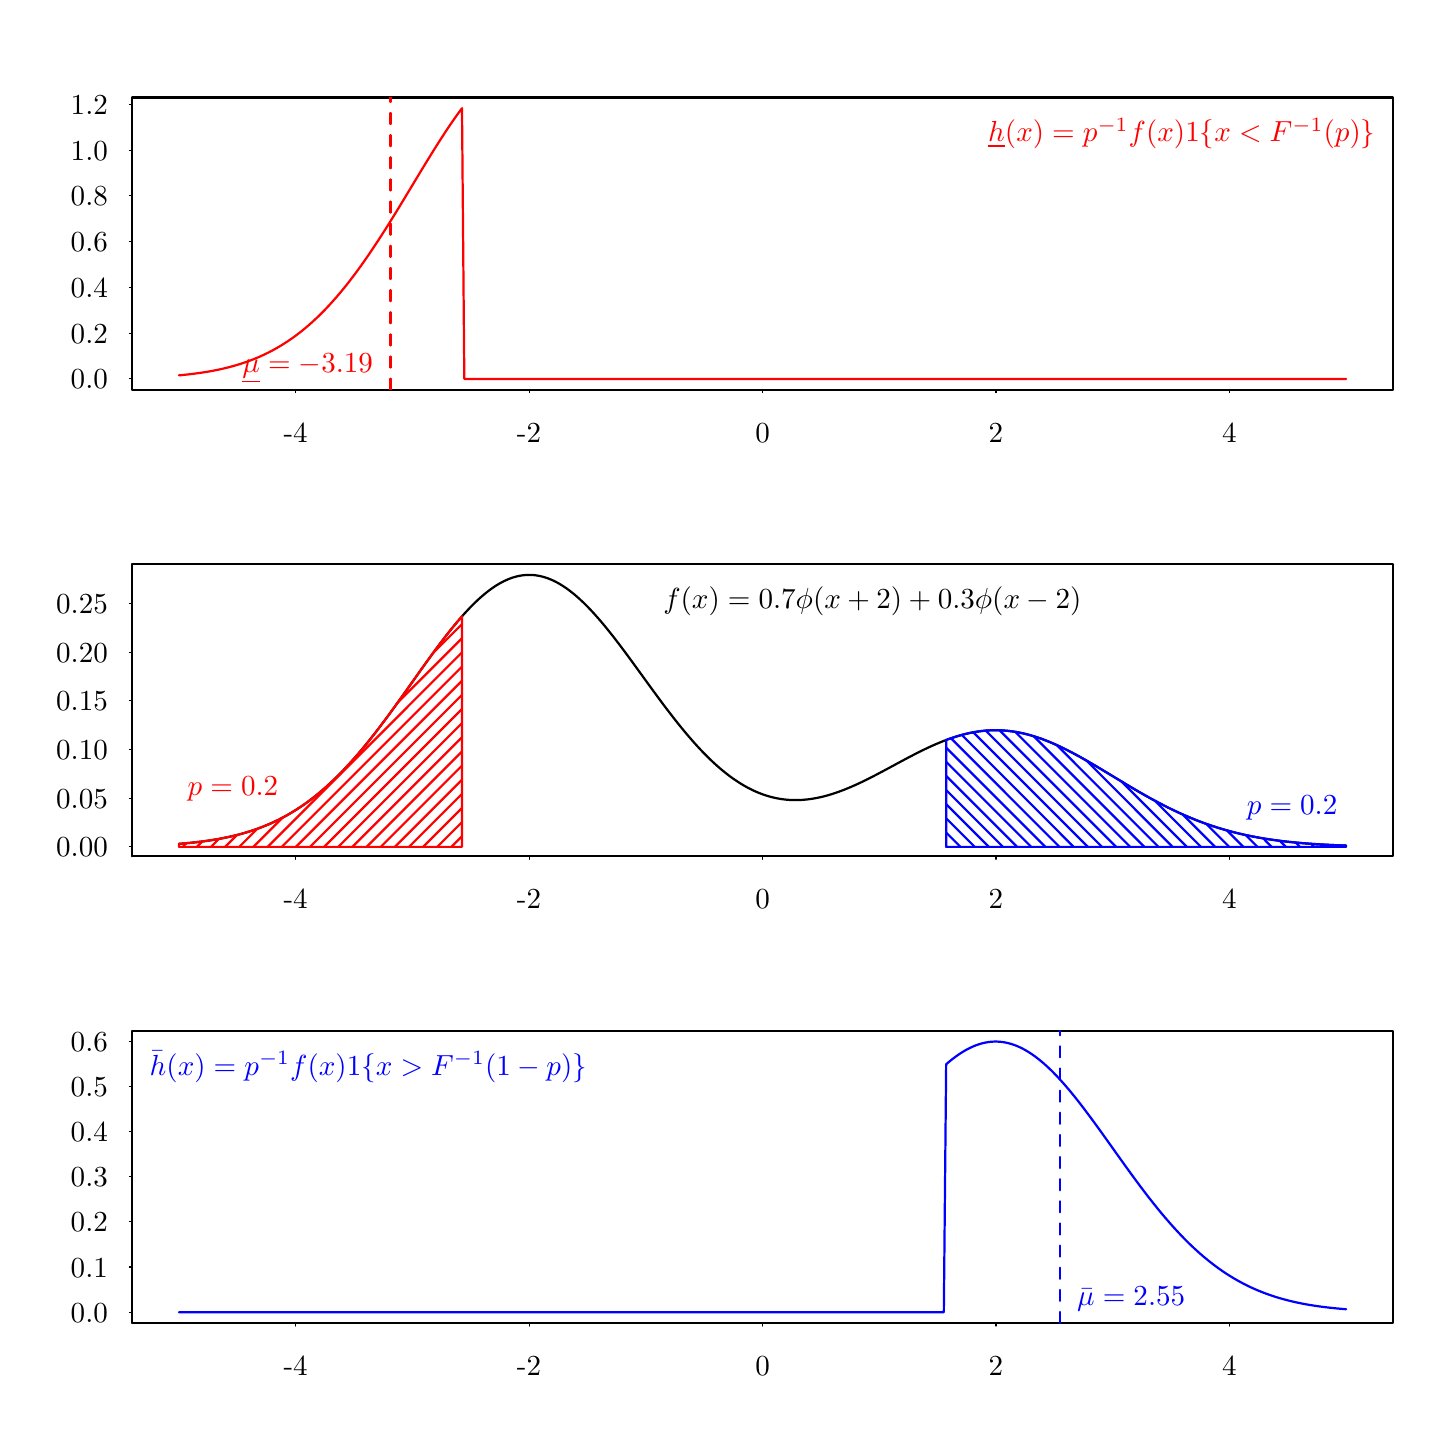
\begin{tikzpicture}[x=1pt,y=1pt]
\definecolor{fillColor}{RGB}{255,255,255}
\path[use as bounding box,fill=fillColor,fill opacity=0.00] (0,0) rectangle (505.89,505.89);
\begin{scope}
\path[clip] ( 37.80,375.06) rectangle (493.29,480.69);
\definecolor{drawColor}{RGB}{255,0,0}

\path[draw=drawColor,line width= 0.8pt,line join=round,line cap=round] ( 54.67,380.25) --
	( 55.52,380.33) --
	( 56.36,380.42) --
	( 57.21,380.50) --
	( 58.05,380.60) --
	( 58.90,380.70) --
	( 59.74,380.80) --
	( 60.59,380.91) --
	( 61.43,381.02) --
	( 62.28,381.14) --
	( 63.12,381.26) --
	( 63.97,381.40) --
	( 64.81,381.53) --
	( 65.66,381.68) --
	( 66.50,381.83) --
	( 67.35,381.99) --
	( 68.19,382.16) --
	( 69.04,382.33) --
	( 69.88,382.52) --
	( 70.73,382.71) --
	( 71.57,382.91) --
	( 72.42,383.12) --
	( 73.26,383.34) --
	( 74.11,383.57) --
	( 74.95,383.81) --
	( 75.80,384.06) --
	( 76.64,384.32) --
	( 77.49,384.59) --
	( 78.34,384.87) --
	( 79.18,385.16) --
	( 80.03,385.47) --
	( 80.87,385.79) --
	( 81.72,386.12) --
	( 82.56,386.46) --
	( 83.41,386.82) --
	( 84.25,387.19) --
	( 85.10,387.58) --
	( 85.94,387.98) --
	( 86.79,388.39) --
	( 87.63,388.82) --
	( 88.48,389.27) --
	( 89.32,389.73) --
	( 90.17,390.21) --
	( 91.01,390.70) --
	( 91.86,391.21) --
	( 92.70,391.74) --
	( 93.55,392.29) --
	( 94.39,392.85) --
	( 95.24,393.43) --
	( 96.08,394.03) --
	( 96.93,394.65) --
	( 97.77,395.29) --
	( 98.62,395.95) --
	( 99.47,396.62) --
	(100.31,397.32) --
	(101.16,398.03) --
	(102.00,398.77) --
	(102.85,399.52) --
	(103.69,400.30) --
	(104.54,401.09) --
	(105.38,401.91) --
	(106.23,402.74) --
	(107.07,403.60) --
	(107.92,404.48) --
	(108.76,405.38) --
	(109.61,406.30) --
	(110.45,407.24) --
	(111.30,408.20) --
	(112.14,409.18) --
	(112.99,410.18) --
	(113.83,411.20) --
	(114.68,412.24) --
	(115.52,413.30) --
	(116.37,414.38) --
	(117.21,415.49) --
	(118.06,416.60) --
	(118.90,417.74) --
	(119.75,418.90) --
	(120.59,420.07) --
	(121.44,421.27) --
	(122.29,422.48) --
	(123.13,423.70) --
	(123.98,424.94) --
	(124.82,426.20) --
	(125.67,427.47) --
	(126.51,428.76) --
	(127.36,430.06) --
	(128.20,431.37) --
	(129.05,432.70) --
	(129.89,434.04) --
	(130.74,435.38) --
	(131.58,436.74) --
	(132.43,438.11) --
	(133.27,439.48) --
	(134.12,440.86) --
	(134.96,442.25) --
	(135.81,443.64) --
	(136.65,445.04) --
	(137.50,446.44) --
	(138.34,447.84) --
	(139.19,449.24) --
	(140.03,450.65) --
	(140.88,452.05) --
	(141.72,453.45) --
	(142.57,454.84) --
	(143.41,456.23) --
	(144.26,457.61) --
	(145.11,458.99) --
	(145.95,460.36) --
	(146.80,461.72) --
	(147.64,463.06) --
	(148.49,464.40) --
	(149.33,465.72) --
	(150.18,467.02) --
	(151.02,468.31) --
	(151.87,469.58) --
	(152.71,470.84) --
	(153.56,472.07) --
	(154.40,473.28) --
	(155.25,474.47) --
	(156.09,475.64) --
	(156.94,476.78) --
	(157.78,378.97) --
	(158.63,378.97) --
	(159.47,378.97) --
	(160.32,378.97) --
	(161.16,378.97) --
	(162.01,378.97) --
	(162.85,378.97) --
	(163.70,378.97) --
	(164.54,378.97) --
	(165.39,378.97) --
	(166.24,378.97) --
	(167.08,378.97) --
	(167.93,378.97) --
	(168.77,378.97) --
	(169.62,378.97) --
	(170.46,378.97) --
	(171.31,378.97) --
	(172.15,378.97) --
	(173.00,378.97) --
	(173.84,378.97) --
	(174.69,378.97) --
	(175.53,378.97) --
	(176.38,378.97) --
	(177.22,378.97) --
	(178.07,378.97) --
	(178.91,378.97) --
	(179.76,378.97) --
	(180.60,378.97) --
	(181.45,378.97) --
	(182.29,378.97) --
	(183.14,378.97) --
	(183.98,378.97) --
	(184.83,378.97) --
	(185.67,378.97) --
	(186.52,378.97) --
	(187.36,378.97) --
	(188.21,378.97) --
	(189.06,378.97) --
	(189.90,378.97) --
	(190.75,378.97) --
	(191.59,378.97) --
	(192.44,378.97) --
	(193.28,378.97) --
	(194.13,378.97) --
	(194.97,378.97) --
	(195.82,378.97) --
	(196.66,378.97) --
	(197.51,378.97) --
	(198.35,378.97) --
	(199.20,378.97) --
	(200.04,378.97) --
	(200.89,378.97) --
	(201.73,378.97) --
	(202.58,378.97) --
	(203.42,378.97) --
	(204.27,378.97) --
	(205.11,378.97) --
	(205.96,378.97) --
	(206.80,378.97) --
	(207.65,378.97) --
	(208.49,378.97) --
	(209.34,378.97) --
	(210.19,378.97) --
	(211.03,378.97) --
	(211.88,378.97) --
	(212.72,378.97) --
	(213.57,378.97) --
	(214.41,378.97) --
	(215.26,378.97) --
	(216.10,378.97) --
	(216.95,378.97) --
	(217.79,378.97) --
	(218.64,378.97) --
	(219.48,378.97) --
	(220.33,378.97) --
	(221.17,378.97) --
	(222.02,378.97) --
	(222.86,378.97) --
	(223.71,378.97) --
	(224.55,378.97) --
	(225.40,378.97) --
	(226.24,378.97) --
	(227.09,378.97) --
	(227.93,378.97) --
	(228.78,378.97) --
	(229.62,378.97) --
	(230.47,378.97) --
	(231.31,378.97) --
	(232.16,378.97) --
	(233.01,378.97) --
	(233.85,378.97) --
	(234.70,378.97) --
	(235.54,378.97) --
	(236.39,378.97) --
	(237.23,378.97) --
	(238.08,378.97) --
	(238.92,378.97) --
	(239.77,378.97) --
	(240.61,378.97) --
	(241.46,378.97) --
	(242.30,378.97) --
	(243.15,378.97) --
	(243.99,378.97) --
	(244.84,378.97) --
	(245.68,378.97) --
	(246.53,378.97) --
	(247.37,378.97) --
	(248.22,378.97) --
	(249.06,378.97) --
	(249.91,378.97) --
	(250.75,378.97) --
	(251.60,378.97) --
	(252.44,378.97) --
	(253.29,378.97) --
	(254.13,378.97) --
	(254.98,378.97) --
	(255.83,378.97) --
	(256.67,378.97) --
	(257.52,378.97) --
	(258.36,378.97) --
	(259.21,378.97) --
	(260.05,378.97) --
	(260.90,378.97) --
	(261.74,378.97) --
	(262.59,378.97) --
	(263.43,378.97) --
	(264.28,378.97) --
	(265.12,378.97) --
	(265.97,378.97) --
	(266.81,378.97) --
	(267.66,378.97) --
	(268.50,378.97) --
	(269.35,378.97) --
	(270.19,378.97) --
	(271.04,378.97) --
	(271.88,378.97) --
	(272.73,378.97) --
	(273.57,378.97) --
	(274.42,378.97) --
	(275.26,378.97) --
	(276.11,378.97) --
	(276.96,378.97) --
	(277.80,378.97) --
	(278.65,378.97) --
	(279.49,378.97) --
	(280.34,378.97) --
	(281.18,378.97) --
	(282.03,378.97) --
	(282.87,378.97) --
	(283.72,378.97) --
	(284.56,378.97) --
	(285.41,378.97) --
	(286.25,378.97) --
	(287.10,378.97) --
	(287.94,378.97) --
	(288.79,378.97) --
	(289.63,378.97) --
	(290.48,378.97) --
	(291.32,378.97) --
	(292.17,378.97) --
	(293.01,378.97) --
	(293.86,378.97) --
	(294.70,378.97) --
	(295.55,378.97) --
	(296.39,378.97) --
	(297.24,378.97) --
	(298.08,378.97) --
	(298.93,378.97) --
	(299.78,378.97) --
	(300.62,378.97) --
	(301.47,378.97) --
	(302.31,378.97) --
	(303.16,378.97) --
	(304.00,378.97) --
	(304.85,378.97) --
	(305.69,378.97) --
	(306.54,378.97) --
	(307.38,378.97) --
	(308.23,378.97) --
	(309.07,378.97) --
	(309.92,378.97) --
	(310.76,378.97) --
	(311.61,378.97) --
	(312.45,378.97) --
	(313.30,378.97) --
	(314.14,378.97) --
	(314.99,378.97) --
	(315.83,378.97) --
	(316.68,378.97) --
	(317.52,378.97) --
	(318.37,378.97) --
	(319.21,378.97) --
	(320.06,378.97) --
	(320.90,378.97) --
	(321.75,378.97) --
	(322.60,378.97) --
	(323.44,378.97) --
	(324.29,378.97) --
	(325.13,378.97) --
	(325.98,378.97) --
	(326.82,378.97) --
	(327.67,378.97) --
	(328.51,378.97) --
	(329.36,378.97) --
	(330.20,378.97) --
	(331.05,378.97) --
	(331.89,378.97) --
	(332.74,378.97) --
	(333.58,378.97) --
	(334.43,378.97) --
	(335.27,378.97) --
	(336.12,378.97) --
	(336.96,378.97) --
	(337.81,378.97) --
	(338.65,378.97) --
	(339.50,378.97) --
	(340.34,378.97) --
	(341.19,378.97) --
	(342.03,378.97) --
	(342.88,378.97) --
	(343.73,378.97) --
	(344.57,378.97) --
	(345.42,378.97) --
	(346.26,378.97) --
	(347.11,378.97) --
	(347.95,378.97) --
	(348.80,378.97) --
	(349.64,378.97) --
	(350.49,378.97) --
	(351.33,378.97) --
	(352.18,378.97) --
	(353.02,378.97) --
	(353.87,378.97) --
	(354.71,378.97) --
	(355.56,378.97) --
	(356.40,378.97) --
	(357.25,378.97) --
	(358.09,378.97) --
	(358.94,378.97) --
	(359.78,378.97) --
	(360.63,378.97) --
	(361.47,378.97) --
	(362.32,378.97) --
	(363.16,378.97) --
	(364.01,378.97) --
	(364.85,378.97) --
	(365.70,378.97) --
	(366.55,378.97) --
	(367.39,378.97) --
	(368.24,378.97) --
	(369.08,378.97) --
	(369.93,378.97) --
	(370.77,378.97) --
	(371.62,378.97) --
	(372.46,378.97) --
	(373.31,378.97) --
	(374.15,378.97) --
	(375.00,378.97) --
	(375.84,378.97) --
	(376.69,378.97) --
	(377.53,378.97) --
	(378.38,378.97) --
	(379.22,378.97) --
	(380.07,378.97) --
	(380.91,378.97) --
	(381.76,378.97) --
	(382.60,378.97) --
	(383.45,378.97) --
	(384.29,378.97) --
	(385.14,378.97) --
	(385.98,378.97) --
	(386.83,378.97) --
	(387.68,378.97) --
	(388.52,378.97) --
	(389.37,378.97) --
	(390.21,378.97) --
	(391.06,378.97) --
	(391.90,378.97) --
	(392.75,378.97) --
	(393.59,378.97) --
	(394.44,378.97) --
	(395.28,378.97) --
	(396.13,378.97) --
	(396.97,378.97) --
	(397.82,378.97) --
	(398.66,378.97) --
	(399.51,378.97) --
	(400.35,378.97) --
	(401.20,378.97) --
	(402.04,378.97) --
	(402.89,378.97) --
	(403.73,378.97) --
	(404.58,378.97) --
	(405.42,378.97) --
	(406.27,378.97) --
	(407.11,378.97) --
	(407.96,378.97) --
	(408.80,378.97) --
	(409.65,378.97) --
	(410.50,378.97) --
	(411.34,378.97) --
	(412.19,378.97) --
	(413.03,378.97) --
	(413.88,378.97) --
	(414.72,378.97) --
	(415.57,378.97) --
	(416.41,378.97) --
	(417.26,378.97) --
	(418.10,378.97) --
	(418.95,378.97) --
	(419.79,378.97) --
	(420.64,378.97) --
	(421.48,378.97) --
	(422.33,378.97) --
	(423.17,378.97) --
	(424.02,378.97) --
	(424.86,378.97) --
	(425.71,378.97) --
	(426.55,378.97) --
	(427.40,378.97) --
	(428.24,378.97) --
	(429.09,378.97) --
	(429.93,378.97) --
	(430.78,378.97) --
	(431.62,378.97) --
	(432.47,378.97) --
	(433.32,378.97) --
	(434.16,378.97) --
	(435.01,378.97) --
	(435.85,378.97) --
	(436.70,378.97) --
	(437.54,378.97) --
	(438.39,378.97) --
	(439.23,378.97) --
	(440.08,378.97) --
	(440.92,378.97) --
	(441.77,378.97) --
	(442.61,378.97) --
	(443.46,378.97) --
	(444.30,378.97) --
	(445.15,378.97) --
	(445.99,378.97) --
	(446.84,378.97) --
	(447.68,378.97) --
	(448.53,378.97) --
	(449.37,378.97) --
	(450.22,378.97) --
	(451.06,378.97) --
	(451.91,378.97) --
	(452.75,378.97) --
	(453.60,378.97) --
	(454.45,378.97) --
	(455.29,378.97) --
	(456.14,378.97) --
	(456.98,378.97) --
	(457.83,378.97) --
	(458.67,378.97) --
	(459.52,378.97) --
	(460.36,378.97) --
	(461.21,378.97) --
	(462.05,378.97) --
	(462.90,378.97) --
	(463.74,378.97) --
	(464.59,378.97) --
	(465.43,378.97) --
	(466.28,378.97) --
	(467.12,378.97) --
	(467.97,378.97) --
	(468.81,378.97) --
	(469.66,378.97) --
	(470.50,378.97) --
	(471.35,378.97) --
	(472.19,378.97) --
	(473.04,378.97) --
	(473.88,378.97) --
	(474.73,378.97) --
	(475.57,378.97) --
	(476.42,378.97);
\end{scope}
\begin{scope}
\path[clip] (  0.00,  0.00) rectangle (505.89,505.89);
\definecolor{drawColor}{RGB}{0,0,0}

\path[draw=drawColor,line width= 0.4pt,line join=round,line cap=round] ( 96.84,375.06) -- (434.25,375.06);

\path[draw=drawColor,line width= 0.4pt,line join=round,line cap=round] ( 96.84,375.06) -- ( 96.84,374.00);

\path[draw=drawColor,line width= 0.4pt,line join=round,line cap=round] (181.19,375.06) -- (181.19,374.00);

\path[draw=drawColor,line width= 0.4pt,line join=round,line cap=round] (265.54,375.06) -- (265.54,374.00);

\path[draw=drawColor,line width= 0.4pt,line join=round,line cap=round] (349.89,375.06) -- (349.89,374.00);

\path[draw=drawColor,line width= 0.4pt,line join=round,line cap=round] (434.25,375.06) -- (434.25,374.00);

\node[text=drawColor,anchor=base,inner sep=0pt, outer sep=0pt, scale=  1.05] at ( 96.84,356.16) {-4};

\node[text=drawColor,anchor=base,inner sep=0pt, outer sep=0pt, scale=  1.05] at (181.19,356.16) {-2};

\node[text=drawColor,anchor=base,inner sep=0pt, outer sep=0pt, scale=  1.05] at (265.54,356.16) {0};

\node[text=drawColor,anchor=base,inner sep=0pt, outer sep=0pt, scale=  1.05] at (349.89,356.16) {2};

\node[text=drawColor,anchor=base,inner sep=0pt, outer sep=0pt, scale=  1.05] at (434.25,356.16) {4};

\path[draw=drawColor,line width= 0.4pt,line join=round,line cap=round] ( 37.80,378.97) -- ( 37.80,478.14);

\path[draw=drawColor,line width= 0.4pt,line join=round,line cap=round] ( 37.80,378.97) -- ( 36.74,378.97);

\path[draw=drawColor,line width= 0.4pt,line join=round,line cap=round] ( 37.80,395.50) -- ( 36.74,395.50);

\path[draw=drawColor,line width= 0.4pt,line join=round,line cap=round] ( 37.80,412.03) -- ( 36.74,412.03);

\path[draw=drawColor,line width= 0.4pt,line join=round,line cap=round] ( 37.80,428.56) -- ( 36.74,428.56);

\path[draw=drawColor,line width= 0.4pt,line join=round,line cap=round] ( 37.80,445.09) -- ( 36.74,445.09);

\path[draw=drawColor,line width= 0.4pt,line join=round,line cap=round] ( 37.80,461.62) -- ( 36.74,461.62);

\path[draw=drawColor,line width= 0.4pt,line join=round,line cap=round] ( 37.80,478.14) -- ( 36.74,478.14);

\node[text=drawColor,anchor=base east,inner sep=0pt, outer sep=0pt, scale=  1.05] at ( 28.98,375.36) {0.0};

\node[text=drawColor,anchor=base east,inner sep=0pt, outer sep=0pt, scale=  1.05] at ( 28.98,391.89) {0.2};

\node[text=drawColor,anchor=base east,inner sep=0pt, outer sep=0pt, scale=  1.05] at ( 28.98,408.41) {0.4};

\node[text=drawColor,anchor=base east,inner sep=0pt, outer sep=0pt, scale=  1.05] at ( 28.98,424.94) {0.6};

\node[text=drawColor,anchor=base east,inner sep=0pt, outer sep=0pt, scale=  1.05] at ( 28.98,441.47) {0.8};

\node[text=drawColor,anchor=base east,inner sep=0pt, outer sep=0pt, scale=  1.05] at ( 28.98,458.00) {1.0};

\node[text=drawColor,anchor=base east,inner sep=0pt, outer sep=0pt, scale=  1.05] at ( 28.98,474.53) {1.2};

\path[draw=drawColor,line width= 0.8pt,line join=round,line cap=round] ( 37.80,375.06) --
	(493.29,375.06) --
	(493.29,480.69) --
	( 37.80,480.69) --
	( 37.80,375.06);
\end{scope}
\begin{scope}
\path[clip] ( 37.80,375.06) rectangle (493.29,480.69);
\definecolor{drawColor}{RGB}{255,0,0}

\node[text=drawColor,anchor=base east,inner sep=0pt, outer sep=0pt, scale=  1.05] at (486.99,464.59) {$\underline{h}(x) = p^{-1}f(x) 1\{x < F^{-1}(p)\}$};

\path[draw=drawColor,line width= 0.8pt,dash pattern=on 4pt off 4pt ,line join=round,line cap=round] (131.07,375.06) -- (131.07,480.69);

\node[text=drawColor,anchor=base east,inner sep=0pt, outer sep=0pt, scale=  1.05] at (124.77,381.45) {$\underline{\mu} = -3.19$};
\end{scope}
\begin{scope}
\path[clip] ( 37.80,206.43) rectangle (493.29,312.06);
\definecolor{drawColor}{RGB}{0,0,0}

\path[draw=drawColor,line width= 0.8pt,line join=round,line cap=round] ( 54.67,210.97) --
	( 55.52,211.03) --
	( 56.36,211.10) --
	( 57.21,211.18) --
	( 58.05,211.26) --
	( 58.90,211.34) --
	( 59.74,211.43) --
	( 60.59,211.52) --
	( 61.43,211.62) --
	( 62.28,211.72) --
	( 63.12,211.83) --
	( 63.97,211.94) --
	( 64.81,212.06) --
	( 65.66,212.18) --
	( 66.50,212.31) --
	( 67.35,212.45) --
	( 68.19,212.59) --
	( 69.04,212.74) --
	( 69.88,212.89) --
	( 70.73,213.06) --
	( 71.57,213.23) --
	( 72.42,213.41) --
	( 73.26,213.59) --
	( 74.11,213.79) --
	( 74.95,213.99) --
	( 75.80,214.20) --
	( 76.64,214.42) --
	( 77.49,214.65) --
	( 78.34,214.90) --
	( 79.18,215.15) --
	( 80.03,215.41) --
	( 80.87,215.68) --
	( 81.72,215.96) --
	( 82.56,216.25) --
	( 83.41,216.56) --
	( 84.25,216.87) --
	( 85.10,217.20) --
	( 85.94,217.54) --
	( 86.79,217.90) --
	( 87.63,218.26) --
	( 88.48,218.64) --
	( 89.32,219.04) --
	( 90.17,219.44) --
	( 91.01,219.86) --
	( 91.86,220.30) --
	( 92.70,220.75) --
	( 93.55,221.21) --
	( 94.39,221.69) --
	( 95.24,222.19) --
	( 96.08,222.70) --
	( 96.93,223.23) --
	( 97.77,223.77) --
	( 98.62,224.33) --
	( 99.47,224.90) --
	(100.31,225.49) --
	(101.16,226.10) --
	(102.00,226.73) --
	(102.85,227.37) --
	(103.69,228.03) --
	(104.54,228.71) --
	(105.38,229.40) --
	(106.23,230.12) --
	(107.07,230.85) --
	(107.92,231.59) --
	(108.76,232.36) --
	(109.61,233.14) --
	(110.45,233.94) --
	(111.30,234.76) --
	(112.14,235.59) --
	(112.99,236.45) --
	(113.83,237.32) --
	(114.68,238.20) --
	(115.52,239.11) --
	(116.37,240.03) --
	(117.21,240.97) --
	(118.06,241.92) --
	(118.90,242.89) --
	(119.75,243.87) --
	(120.59,244.87) --
	(121.44,245.89) --
	(122.29,246.92) --
	(123.13,247.96) --
	(123.98,249.02) --
	(124.82,250.09) --
	(125.67,251.17) --
	(126.51,252.27) --
	(127.36,253.38) --
	(128.20,254.50) --
	(129.05,255.62) --
	(129.89,256.76) --
	(130.74,257.91) --
	(131.58,259.07) --
	(132.43,260.23) --
	(133.27,261.40) --
	(134.12,262.58) --
	(134.96,263.76) --
	(135.81,264.94) --
	(136.65,266.13) --
	(137.50,267.32) --
	(138.34,268.52) --
	(139.19,269.71) --
	(140.03,270.91) --
	(140.88,272.10) --
	(141.72,273.29) --
	(142.57,274.48) --
	(143.41,275.66) --
	(144.26,276.84) --
	(145.11,278.01) --
	(145.95,279.18) --
	(146.80,280.33) --
	(147.64,281.48) --
	(148.49,282.61) --
	(149.33,283.74) --
	(150.18,284.85) --
	(151.02,285.95) --
	(151.87,287.03) --
	(152.71,288.10) --
	(153.56,289.15) --
	(154.40,290.18) --
	(155.25,291.19) --
	(156.09,292.19) --
	(156.94,293.16) --
	(157.78,294.11) --
	(158.63,295.03) --
	(159.47,295.93) --
	(160.32,296.81) --
	(161.16,297.66) --
	(162.01,298.48) --
	(162.85,299.27) --
	(163.70,300.04) --
	(164.54,300.77) --
	(165.39,301.47) --
	(166.24,302.15) --
	(167.08,302.79) --
	(167.93,303.39) --
	(168.77,303.97) --
	(169.62,304.51) --
	(170.46,305.01) --
	(171.31,305.48) --
	(172.15,305.91) --
	(173.00,306.30) --
	(173.84,306.66) --
	(174.69,306.98) --
	(175.53,307.26) --
	(176.38,307.50) --
	(177.22,307.71) --
	(178.07,307.88) --
	(178.91,308.00) --
	(179.76,308.09) --
	(180.60,308.14) --
	(181.45,308.15) --
	(182.29,308.12) --
	(183.14,308.05) --
	(183.98,307.94) --
	(184.83,307.79) --
	(185.67,307.60) --
	(186.52,307.38) --
	(187.36,307.11) --
	(188.21,306.81) --
	(189.06,306.47) --
	(189.90,306.10) --
	(190.75,305.68) --
	(191.59,305.23) --
	(192.44,304.75) --
	(193.28,304.22) --
	(194.13,303.67) --
	(194.97,303.08) --
	(195.82,302.46) --
	(196.66,301.80) --
	(197.51,301.12) --
	(198.35,300.40) --
	(199.20,299.65) --
	(200.04,298.87) --
	(200.89,298.07) --
	(201.73,297.24) --
	(202.58,296.38) --
	(203.42,295.49) --
	(204.27,294.59) --
	(205.11,293.65) --
	(205.96,292.70) --
	(206.80,291.73) --
	(207.65,290.73) --
	(208.49,289.72) --
	(209.34,288.68) --
	(210.19,287.63) --
	(211.03,286.57) --
	(211.88,285.49) --
	(212.72,284.40) --
	(213.57,283.29) --
	(214.41,282.18) --
	(215.26,281.05) --
	(216.10,279.91) --
	(216.95,278.77) --
	(217.79,277.62) --
	(218.64,276.46) --
	(219.48,275.30) --
	(220.33,274.14) --
	(221.17,272.97) --
	(222.02,271.81) --
	(222.86,270.64) --
	(223.71,269.47) --
	(224.55,268.31) --
	(225.40,267.15) --
	(226.24,265.99) --
	(227.09,264.84) --
	(227.93,263.69) --
	(228.78,262.55) --
	(229.62,261.42) --
	(230.47,260.29) --
	(231.31,259.18) --
	(232.16,258.08) --
	(233.01,256.98) --
	(233.85,255.90) --
	(234.70,254.83) --
	(235.54,253.78) --
	(236.39,252.74) --
	(237.23,251.71) --
	(238.08,250.70) --
	(238.92,249.71) --
	(239.77,248.73) --
	(240.61,247.77) --
	(241.46,246.82) --
	(242.30,245.90) --
	(243.15,244.99) --
	(243.99,244.10) --
	(244.84,243.24) --
	(245.68,242.39) --
	(246.53,241.56) --
	(247.37,240.76) --
	(248.22,239.97) --
	(249.06,239.21) --
	(249.91,238.47) --
	(250.75,237.75) --
	(251.60,237.05) --
	(252.44,236.38) --
	(253.29,235.73) --
	(254.13,235.10) --
	(254.98,234.49) --
	(255.83,233.91) --
	(256.67,233.35) --
	(257.52,232.81) --
	(258.36,232.30) --
	(259.21,231.81) --
	(260.05,231.34) --
	(260.90,230.90) --
	(261.74,230.48) --
	(262.59,230.08) --
	(263.43,229.70) --
	(264.28,229.35) --
	(265.12,229.03) --
	(265.97,228.72) --
	(266.81,228.44) --
	(267.66,228.18) --
	(268.50,227.94) --
	(269.35,227.73) --
	(270.19,227.54) --
	(271.04,227.37) --
	(271.88,227.22) --
	(272.73,227.09) --
	(273.57,226.99) --
	(274.42,226.90) --
	(275.26,226.84) --
	(276.11,226.80) --
	(276.96,226.78) --
	(277.80,226.77) --
	(278.65,226.79) --
	(279.49,226.83) --
	(280.34,226.88) --
	(281.18,226.96) --
	(282.03,227.05) --
	(282.87,227.16) --
	(283.72,227.29) --
	(284.56,227.44) --
	(285.41,227.60) --
	(286.25,227.78) --
	(287.10,227.97) --
	(287.94,228.18) --
	(288.79,228.41) --
	(289.63,228.65) --
	(290.48,228.91) --
	(291.32,229.18) --
	(292.17,229.46) --
	(293.01,229.76) --
	(293.86,230.07) --
	(294.70,230.39) --
	(295.55,230.72) --
	(296.39,231.07) --
	(297.24,231.42) --
	(298.08,231.79) --
	(298.93,232.16) --
	(299.78,232.55) --
	(300.62,232.94) --
	(301.47,233.34) --
	(302.31,233.75) --
	(303.16,234.16) --
	(304.00,234.59) --
	(304.85,235.01) --
	(305.69,235.45) --
	(306.54,235.89) --
	(307.38,236.33) --
	(308.23,236.78) --
	(309.07,237.23) --
	(309.92,237.68) --
	(310.76,238.13) --
	(311.61,238.59) --
	(312.45,239.05) --
	(313.30,239.50) --
	(314.14,239.96) --
	(314.99,240.41) --
	(315.83,240.87) --
	(316.68,241.32) --
	(317.52,241.77) --
	(318.37,242.22) --
	(319.21,242.66) --
	(320.06,243.10) --
	(320.90,243.53) --
	(321.75,243.96) --
	(322.60,244.38) --
	(323.44,244.80) --
	(324.29,245.21) --
	(325.13,245.61) --
	(325.98,246.00) --
	(326.82,246.39) --
	(327.67,246.76) --
	(328.51,247.13) --
	(329.36,247.48) --
	(330.20,247.83) --
	(331.05,248.16) --
	(331.89,248.49) --
	(332.74,248.80) --
	(333.58,249.09) --
	(334.43,249.38) --
	(335.27,249.65) --
	(336.12,249.91) --
	(336.96,250.16) --
	(337.81,250.39) --
	(338.65,250.61) --
	(339.50,250.81) --
	(340.34,251.00) --
	(341.19,251.17) --
	(342.03,251.33) --
	(342.88,251.47) --
	(343.73,251.60) --
	(344.57,251.71) --
	(345.42,251.80) --
	(346.26,251.88) --
	(347.11,251.94) --
	(347.95,251.98) --
	(348.80,252.01) --
	(349.64,252.02) --
	(350.49,252.01) --
	(351.33,251.99) --
	(352.18,251.95) --
	(353.02,251.89) --
	(353.87,251.82) --
	(354.71,251.73) --
	(355.56,251.63) --
	(356.40,251.51) --
	(357.25,251.37) --
	(358.09,251.21) --
	(358.94,251.04) --
	(359.78,250.86) --
	(360.63,250.66) --
	(361.47,250.44) --
	(362.32,250.21) --
	(363.16,249.96) --
	(364.01,249.70) --
	(364.85,249.43) --
	(365.70,249.14) --
	(366.55,248.84) --
	(367.39,248.52) --
	(368.24,248.19) --
	(369.08,247.85) --
	(369.93,247.50) --
	(370.77,247.13) --
	(371.62,246.76) --
	(372.46,246.37) --
	(373.31,245.98) --
	(374.15,245.57) --
	(375.00,245.15) --
	(375.84,244.73) --
	(376.69,244.29) --
	(377.53,243.85) --
	(378.38,243.40) --
	(379.22,242.94) --
	(380.07,242.48) --
	(380.91,242.01) --
	(381.76,241.53) --
	(382.60,241.05) --
	(383.45,240.56) --
	(384.29,240.07) --
	(385.14,239.58) --
	(385.98,239.08) --
	(386.83,238.57) --
	(387.68,238.07) --
	(388.52,237.56) --
	(389.37,237.05) --
	(390.21,236.54) --
	(391.06,236.03) --
	(391.90,235.52) --
	(392.75,235.01) --
	(393.59,234.50) --
	(394.44,233.98) --
	(395.28,233.48) --
	(396.13,232.97) --
	(396.97,232.46) --
	(397.82,231.96) --
	(398.66,231.46) --
	(399.51,230.96) --
	(400.35,230.46) --
	(401.20,229.97) --
	(402.04,229.48) --
	(402.89,229.00) --
	(403.73,228.52) --
	(404.58,228.04) --
	(405.42,227.57) --
	(406.27,227.11) --
	(407.11,226.65) --
	(407.96,226.20) --
	(408.80,225.75) --
	(409.65,225.31) --
	(410.50,224.87) --
	(411.34,224.45) --
	(412.19,224.02) --
	(413.03,223.61) --
	(413.88,223.20) --
	(414.72,222.80) --
	(415.57,222.40) --
	(416.41,222.02) --
	(417.26,221.64) --
	(418.10,221.26) --
	(418.95,220.90) --
	(419.79,220.54) --
	(420.64,220.19) --
	(421.48,219.85) --
	(422.33,219.51) --
	(423.17,219.18) --
	(424.02,218.86) --
	(424.86,218.55) --
	(425.71,218.24) --
	(426.55,217.95) --
	(427.40,217.66) --
	(428.24,217.37) --
	(429.09,217.10) --
	(429.93,216.83) --
	(430.78,216.57) --
	(431.62,216.32) --
	(432.47,216.07) --
	(433.32,215.83) --
	(434.16,215.60) --
	(435.01,215.37) --
	(435.85,215.15) --
	(436.70,214.94) --
	(437.54,214.73) --
	(438.39,214.53) --
	(439.23,214.34) --
	(440.08,214.16) --
	(440.92,213.98) --
	(441.77,213.80) --
	(442.61,213.63) --
	(443.46,213.47) --
	(444.30,213.31) --
	(445.15,213.16) --
	(445.99,213.02) --
	(446.84,212.87) --
	(447.68,212.74) --
	(448.53,212.61) --
	(449.37,212.48) --
	(450.22,212.36) --
	(451.06,212.25) --
	(451.91,212.13) --
	(452.75,212.03) --
	(453.60,211.92) --
	(454.45,211.82) --
	(455.29,211.73) --
	(456.14,211.64) --
	(456.98,211.55) --
	(457.83,211.47) --
	(458.67,211.39) --
	(459.52,211.31) --
	(460.36,211.24) --
	(461.21,211.17) --
	(462.05,211.10) --
	(462.90,211.04) --
	(463.74,210.98) --
	(464.59,210.92) --
	(465.43,210.86) --
	(466.28,210.81) --
	(467.12,210.76) --
	(467.97,210.71) --
	(468.81,210.67) --
	(469.66,210.62) --
	(470.50,210.58) --
	(471.35,210.54) --
	(472.19,210.50) --
	(473.04,210.47) --
	(473.88,210.43) --
	(474.73,210.40) --
	(475.57,210.37) --
	(476.42,210.34);
\end{scope}
\begin{scope}
\path[clip] (  0.00,  0.00) rectangle (505.89,505.89);
\definecolor{drawColor}{RGB}{0,0,0}

\path[draw=drawColor,line width= 0.4pt,line join=round,line cap=round] ( 96.84,206.43) -- (434.25,206.43);

\path[draw=drawColor,line width= 0.4pt,line join=round,line cap=round] ( 96.84,206.43) -- ( 96.84,205.37);

\path[draw=drawColor,line width= 0.4pt,line join=round,line cap=round] (181.19,206.43) -- (181.19,205.37);

\path[draw=drawColor,line width= 0.4pt,line join=round,line cap=round] (265.54,206.43) -- (265.54,205.37);

\path[draw=drawColor,line width= 0.4pt,line join=round,line cap=round] (349.89,206.43) -- (349.89,205.37);

\path[draw=drawColor,line width= 0.4pt,line join=round,line cap=round] (434.25,206.43) -- (434.25,205.37);

\node[text=drawColor,anchor=base,inner sep=0pt, outer sep=0pt, scale=  1.05] at ( 96.84,187.53) {-4};

\node[text=drawColor,anchor=base,inner sep=0pt, outer sep=0pt, scale=  1.05] at (181.19,187.53) {-2};

\node[text=drawColor,anchor=base,inner sep=0pt, outer sep=0pt, scale=  1.05] at (265.54,187.53) {0};

\node[text=drawColor,anchor=base,inner sep=0pt, outer sep=0pt, scale=  1.05] at (349.89,187.53) {2};

\node[text=drawColor,anchor=base,inner sep=0pt, outer sep=0pt, scale=  1.05] at (434.25,187.53) {4};

\path[draw=drawColor,line width= 0.4pt,line join=round,line cap=round] ( 37.80,209.87) -- ( 37.80,297.84);

\path[draw=drawColor,line width= 0.4pt,line join=round,line cap=round] ( 37.80,209.87) -- ( 36.74,209.87);

\path[draw=drawColor,line width= 0.4pt,line join=round,line cap=round] ( 37.80,227.47) -- ( 36.74,227.47);

\path[draw=drawColor,line width= 0.4pt,line join=round,line cap=round] ( 37.80,245.06) -- ( 36.74,245.06);

\path[draw=drawColor,line width= 0.4pt,line join=round,line cap=round] ( 37.80,262.65) -- ( 36.74,262.65);

\path[draw=drawColor,line width= 0.4pt,line join=round,line cap=round] ( 37.80,280.25) -- ( 36.74,280.25);

\path[draw=drawColor,line width= 0.4pt,line join=round,line cap=round] ( 37.80,297.84) -- ( 36.74,297.84);

\node[text=drawColor,anchor=base east,inner sep=0pt, outer sep=0pt, scale=  1.05] at ( 28.98,206.26) {0.00};

\node[text=drawColor,anchor=base east,inner sep=0pt, outer sep=0pt, scale=  1.05] at ( 28.98,223.85) {0.05};

\node[text=drawColor,anchor=base east,inner sep=0pt, outer sep=0pt, scale=  1.05] at ( 28.98,241.44) {0.10};

\node[text=drawColor,anchor=base east,inner sep=0pt, outer sep=0pt, scale=  1.05] at ( 28.98,259.04) {0.15};

\node[text=drawColor,anchor=base east,inner sep=0pt, outer sep=0pt, scale=  1.05] at ( 28.98,276.63) {0.20};

\node[text=drawColor,anchor=base east,inner sep=0pt, outer sep=0pt, scale=  1.05] at ( 28.98,294.22) {0.25};

\path[draw=drawColor,line width= 0.8pt,line join=round,line cap=round] ( 37.80,206.43) --
	(493.29,206.43) --
	(493.29,312.06) --
	( 37.80,312.06) --
	( 37.80,206.43);
\end{scope}
\begin{scope}
\path[clip] ( 37.80,206.43) rectangle (493.29,312.06);
\definecolor{drawColor}{RGB}{255,0,0}

\path[draw=drawColor,line width= 0.8pt,line join=round,line cap=round] ( 56.02,209.87) -- ( 57.34,211.19);

\path[draw=drawColor,line width= 0.8pt,line join=round,line cap=round] ( 61.13,209.87) -- ( 63.08,211.82);

\path[draw=drawColor,line width= 0.8pt,line join=round,line cap=round] ( 66.24,209.87) -- ( 69.12,212.75);

\path[draw=drawColor,line width= 0.8pt,line join=round,line cap=round] ( 71.36,209.87) -- ( 75.64,214.16);

\path[draw=drawColor,line width= 0.8pt,line join=round,line cap=round] ( 76.47,209.87) -- ( 83.00,216.41);

\path[draw=drawColor,line width= 0.8pt,line join=round,line cap=round] (146.45,279.86) -- (156.94,290.35);

\path[draw=drawColor,line width= 0.8pt,line join=round,line cap=round] ( 81.58,209.87) -- ( 92.16,220.46);

\path[draw=drawColor,line width= 0.8pt,line join=round,line cap=round] (133.71,262.01) -- (156.94,285.24);

\path[draw=drawColor,line width= 0.8pt,line join=round,line cap=round] ( 86.69,209.87) -- (156.94,280.13);

\path[draw=drawColor,line width= 0.8pt,line join=round,line cap=round] ( 91.80,209.87) -- (156.94,275.02);

\path[draw=drawColor,line width= 0.8pt,line join=round,line cap=round] ( 96.91,209.87) -- (156.94,269.91);

\path[draw=drawColor,line width= 0.8pt,line join=round,line cap=round] (102.02,209.87) -- (156.94,264.80);

\path[draw=drawColor,line width= 0.8pt,line join=round,line cap=round] (107.13,209.87) -- (156.94,259.69);

\path[draw=drawColor,line width= 0.8pt,line join=round,line cap=round] (112.24,209.87) -- (156.94,254.58);

\path[draw=drawColor,line width= 0.8pt,line join=round,line cap=round] (117.35,209.87) -- (156.94,249.46);

\path[draw=drawColor,line width= 0.8pt,line join=round,line cap=round] (122.46,209.87) -- (156.94,244.35);

\path[draw=drawColor,line width= 0.8pt,line join=round,line cap=round] (127.57,209.87) -- (156.94,239.24);

\path[draw=drawColor,line width= 0.8pt,line join=round,line cap=round] (132.68,209.87) -- (156.94,234.13);

\path[draw=drawColor,line width= 0.8pt,line join=round,line cap=round] (137.79,209.87) -- (156.94,229.02);

\path[draw=drawColor,line width= 0.8pt,line join=round,line cap=round] (142.90,209.87) -- (156.94,223.91);

\path[draw=drawColor,line width= 0.8pt,line join=round,line cap=round] (148.01,209.87) -- (156.94,218.80);

\path[draw=drawColor,line width= 0.8pt,line join=round,line cap=round] (153.12,209.87) -- (156.94,213.69);

\path[draw=drawColor,line width= 0.8pt,line join=round,line cap=round] ( 54.67,209.87) --
	( 55.52,209.87) --
	( 56.36,209.87) --
	( 57.21,209.87) --
	( 58.05,209.87) --
	( 58.90,209.87) --
	( 59.74,209.87) --
	( 60.59,209.87) --
	( 61.43,209.87) --
	( 62.28,209.87) --
	( 63.12,209.87) --
	( 63.97,209.87) --
	( 64.81,209.87) --
	( 65.66,209.87) --
	( 66.50,209.87) --
	( 67.35,209.87) --
	( 68.19,209.87) --
	( 69.04,209.87) --
	( 69.88,209.87) --
	( 70.73,209.87) --
	( 71.57,209.87) --
	( 72.42,209.87) --
	( 73.26,209.87) --
	( 74.11,209.87) --
	( 74.95,209.87) --
	( 75.80,209.87) --
	( 76.64,209.87) --
	( 77.49,209.87) --
	( 78.34,209.87) --
	( 79.18,209.87) --
	( 80.03,209.87) --
	( 80.87,209.87) --
	( 81.72,209.87) --
	( 82.56,209.87) --
	( 83.41,209.87) --
	( 84.25,209.87) --
	( 85.10,209.87) --
	( 85.94,209.87) --
	( 86.79,209.87) --
	( 87.63,209.87) --
	( 88.48,209.87) --
	( 89.32,209.87) --
	( 90.17,209.87) --
	( 91.01,209.87) --
	( 91.86,209.87) --
	( 92.70,209.87) --
	( 93.55,209.87) --
	( 94.39,209.87) --
	( 95.24,209.87) --
	( 96.08,209.87) --
	( 96.93,209.87) --
	( 97.77,209.87) --
	( 98.62,209.87) --
	( 99.47,209.87) --
	(100.31,209.87) --
	(101.16,209.87) --
	(102.00,209.87) --
	(102.85,209.87) --
	(103.69,209.87) --
	(104.54,209.87) --
	(105.38,209.87) --
	(106.23,209.87) --
	(107.07,209.87) --
	(107.92,209.87) --
	(108.76,209.87) --
	(109.61,209.87) --
	(110.45,209.87) --
	(111.30,209.87) --
	(112.14,209.87) --
	(112.99,209.87) --
	(113.83,209.87) --
	(114.68,209.87) --
	(115.52,209.87) --
	(116.37,209.87) --
	(117.21,209.87) --
	(118.06,209.87) --
	(118.90,209.87) --
	(119.75,209.87) --
	(120.59,209.87) --
	(121.44,209.87) --
	(122.29,209.87) --
	(123.13,209.87) --
	(123.98,209.87) --
	(124.82,209.87) --
	(125.67,209.87) --
	(126.51,209.87) --
	(127.36,209.87) --
	(128.20,209.87) --
	(129.05,209.87) --
	(129.89,209.87) --
	(130.74,209.87) --
	(131.58,209.87) --
	(132.43,209.87) --
	(133.27,209.87) --
	(134.12,209.87) --
	(134.96,209.87) --
	(135.81,209.87) --
	(136.65,209.87) --
	(137.50,209.87) --
	(138.34,209.87) --
	(139.19,209.87) --
	(140.03,209.87) --
	(140.88,209.87) --
	(141.72,209.87) --
	(142.57,209.87) --
	(143.41,209.87) --
	(144.26,209.87) --
	(145.11,209.87) --
	(145.95,209.87) --
	(146.80,209.87) --
	(147.64,209.87) --
	(148.49,209.87) --
	(149.33,209.87) --
	(150.18,209.87) --
	(151.02,209.87) --
	(151.87,209.87) --
	(152.71,209.87) --
	(153.56,209.87) --
	(154.40,209.87) --
	(155.25,209.87) --
	(156.09,209.87) --
	(156.94,209.87) --
	(156.94,293.16) --
	(156.09,292.19) --
	(155.25,291.19) --
	(154.40,290.18) --
	(153.56,289.15) --
	(152.71,288.10) --
	(151.87,287.03) --
	(151.02,285.95) --
	(150.18,284.85) --
	(149.33,283.74) --
	(148.49,282.61) --
	(147.64,281.48) --
	(146.80,280.33) --
	(145.95,279.18) --
	(145.11,278.01) --
	(144.26,276.84) --
	(143.41,275.66) --
	(142.57,274.48) --
	(141.72,273.29) --
	(140.88,272.10) --
	(140.03,270.91) --
	(139.19,269.71) --
	(138.34,268.52) --
	(137.50,267.32) --
	(136.65,266.13) --
	(135.81,264.94) --
	(134.96,263.76) --
	(134.12,262.58) --
	(133.27,261.40) --
	(132.43,260.23) --
	(131.58,259.07) --
	(130.74,257.91) --
	(129.89,256.76) --
	(129.05,255.62) --
	(128.20,254.50) --
	(127.36,253.38) --
	(126.51,252.27) --
	(125.67,251.17) --
	(124.82,250.09) --
	(123.98,249.02) --
	(123.13,247.96) --
	(122.29,246.92) --
	(121.44,245.89) --
	(120.59,244.87) --
	(119.75,243.87) --
	(118.90,242.89) --
	(118.06,241.92) --
	(117.21,240.97) --
	(116.37,240.03) --
	(115.52,239.11) --
	(114.68,238.20) --
	(113.83,237.32) --
	(112.99,236.45) --
	(112.14,235.59) --
	(111.30,234.76) --
	(110.45,233.94) --
	(109.61,233.14) --
	(108.76,232.36) --
	(107.92,231.59) --
	(107.07,230.85) --
	(106.23,230.12) --
	(105.38,229.40) --
	(104.54,228.71) --
	(103.69,228.03) --
	(102.85,227.37) --
	(102.00,226.73) --
	(101.16,226.10) --
	(100.31,225.49) --
	( 99.47,224.90) --
	( 98.62,224.33) --
	( 97.77,223.77) --
	( 96.93,223.23) --
	( 96.08,222.70) --
	( 95.24,222.19) --
	( 94.39,221.69) --
	( 93.55,221.21) --
	( 92.70,220.75) --
	( 91.86,220.30) --
	( 91.01,219.86) --
	( 90.17,219.44) --
	( 89.32,219.04) --
	( 88.48,218.64) --
	( 87.63,218.26) --
	( 86.79,217.90) --
	( 85.94,217.54) --
	( 85.10,217.20) --
	( 84.25,216.87) --
	( 83.41,216.56) --
	( 82.56,216.25) --
	( 81.72,215.96) --
	( 80.87,215.68) --
	( 80.03,215.41) --
	( 79.18,215.15) --
	( 78.34,214.90) --
	( 77.49,214.65) --
	( 76.64,214.42) --
	( 75.80,214.20) --
	( 74.95,213.99) --
	( 74.11,213.79) --
	( 73.26,213.59) --
	( 72.42,213.41) --
	( 71.57,213.23) --
	( 70.73,213.06) --
	( 69.88,212.89) --
	( 69.04,212.74) --
	( 68.19,212.59) --
	( 67.35,212.45) --
	( 66.50,212.31) --
	( 65.66,212.18) --
	( 64.81,212.06) --
	( 63.97,211.94) --
	( 63.12,211.83) --
	( 62.28,211.72) --
	( 61.43,211.62) --
	( 60.59,211.52) --
	( 59.74,211.43) --
	( 58.90,211.34) --
	( 58.05,211.26) --
	( 57.21,211.18) --
	( 56.36,211.10) --
	( 55.52,211.03) --
	( 54.67,210.97) --
	( 54.67,209.87);

\node[text=drawColor,anchor=base east,inner sep=0pt, outer sep=0pt, scale=  1.05] at ( 90.54,228.58) {$p = 0.2$};
\definecolor{drawColor}{RGB}{0,0,255}

\path[draw=drawColor,line width= 0.8pt,line join=round,line cap=round] (331.98,209.87) -- (331.89,209.96);

\path[draw=drawColor,line width= 0.8pt,line join=round,line cap=round] (337.09,209.87) -- (331.89,215.07);

\path[draw=drawColor,line width= 0.8pt,line join=round,line cap=round] (342.20,209.87) -- (331.89,220.18);

\path[draw=drawColor,line width= 0.8pt,line join=round,line cap=round] (347.31,209.87) -- (331.89,225.29);

\path[draw=drawColor,line width= 0.8pt,line join=round,line cap=round] (352.42,209.87) -- (331.89,230.40);

\path[draw=drawColor,line width= 0.8pt,line join=round,line cap=round] (357.53,209.87) -- (331.89,235.51);

\path[draw=drawColor,line width= 0.8pt,line join=round,line cap=round] (362.64,209.87) -- (331.89,240.62);

\path[draw=drawColor,line width= 0.8pt,line join=round,line cap=round] (367.75,209.87) -- (331.89,245.73);

\path[draw=drawColor,line width= 0.8pt,line join=round,line cap=round] (372.86,209.87) -- (333.63,249.11);

\path[draw=drawColor,line width= 0.8pt,line join=round,line cap=round] (377.97,209.87) -- (337.53,250.32);

\path[draw=drawColor,line width= 0.8pt,line join=round,line cap=round] (383.08,209.87) -- (341.69,251.27);

\path[draw=drawColor,line width= 0.8pt,line join=round,line cap=round] (388.19,209.87) -- (346.20,251.87);

\path[draw=drawColor,line width= 0.8pt,line join=round,line cap=round] (393.30,209.87) -- (351.18,251.99);

\path[draw=drawColor,line width= 0.8pt,line join=round,line cap=round] (398.41,209.87) -- (356.85,251.43);

\path[draw=drawColor,line width= 0.8pt,line join=round,line cap=round] (403.52,209.87) -- (363.56,249.84);

\path[draw=drawColor,line width= 0.8pt,line join=round,line cap=round] (408.63,209.87) -- (371.86,246.65);

\path[draw=drawColor,line width= 0.8pt,line join=round,line cap=round] (413.74,209.87) -- (382.52,241.10);

\path[draw=drawColor,line width= 0.8pt,line join=round,line cap=round] (418.85,209.87) -- (395.21,233.52);

\path[draw=drawColor,line width= 0.8pt,line join=round,line cap=round] (423.96,209.87) -- (407.27,226.57);

\path[draw=drawColor,line width= 0.8pt,line join=round,line cap=round] (429.07,209.87) -- (417.36,221.59);

\path[draw=drawColor,line width= 0.8pt,line join=round,line cap=round] (434.18,209.87) -- (425.87,218.19);

\path[draw=drawColor,line width= 0.8pt,line join=round,line cap=round] (439.29,209.87) -- (433.35,215.82);

\path[draw=drawColor,line width= 0.8pt,line join=round,line cap=round] (444.40,209.87) -- (440.14,214.14);

\path[draw=drawColor,line width= 0.8pt,line join=round,line cap=round] (449.51,209.87) -- (446.45,212.94);

\path[draw=drawColor,line width= 0.8pt,line join=round,line cap=round] (454.62,209.87) -- (452.43,212.07);

\path[draw=drawColor,line width= 0.8pt,line join=round,line cap=round] (459.73,209.87) -- (458.17,211.43);

\path[draw=drawColor,line width= 0.8pt,line join=round,line cap=round] (464.85,209.87) -- (463.74,210.98);

\path[draw=drawColor,line width= 0.8pt,line join=round,line cap=round] (469.96,209.87) -- (469.18,210.65);

\path[draw=drawColor,line width= 0.8pt,line join=round,line cap=round] (475.07,209.87) -- (474.53,210.41);

\path[draw=drawColor,line width= 0.8pt,line join=round,line cap=round] (331.89,209.87) --
	(332.74,209.87) --
	(333.58,209.87) --
	(334.43,209.87) --
	(335.27,209.87) --
	(336.12,209.87) --
	(336.96,209.87) --
	(337.81,209.87) --
	(338.65,209.87) --
	(339.50,209.87) --
	(340.34,209.87) --
	(341.19,209.87) --
	(342.03,209.87) --
	(342.88,209.87) --
	(343.73,209.87) --
	(344.57,209.87) --
	(345.42,209.87) --
	(346.26,209.87) --
	(347.11,209.87) --
	(347.95,209.87) --
	(348.80,209.87) --
	(349.64,209.87) --
	(350.49,209.87) --
	(351.33,209.87) --
	(352.18,209.87) --
	(353.02,209.87) --
	(353.87,209.87) --
	(354.71,209.87) --
	(355.56,209.87) --
	(356.40,209.87) --
	(357.25,209.87) --
	(358.09,209.87) --
	(358.94,209.87) --
	(359.78,209.87) --
	(360.63,209.87) --
	(361.47,209.87) --
	(362.32,209.87) --
	(363.16,209.87) --
	(364.01,209.87) --
	(364.85,209.87) --
	(365.70,209.87) --
	(366.55,209.87) --
	(367.39,209.87) --
	(368.24,209.87) --
	(369.08,209.87) --
	(369.93,209.87) --
	(370.77,209.87) --
	(371.62,209.87) --
	(372.46,209.87) --
	(373.31,209.87) --
	(374.15,209.87) --
	(375.00,209.87) --
	(375.84,209.87) --
	(376.69,209.87) --
	(377.53,209.87) --
	(378.38,209.87) --
	(379.22,209.87) --
	(380.07,209.87) --
	(380.91,209.87) --
	(381.76,209.87) --
	(382.60,209.87) --
	(383.45,209.87) --
	(384.29,209.87) --
	(385.14,209.87) --
	(385.98,209.87) --
	(386.83,209.87) --
	(387.68,209.87) --
	(388.52,209.87) --
	(389.37,209.87) --
	(390.21,209.87) --
	(391.06,209.87) --
	(391.90,209.87) --
	(392.75,209.87) --
	(393.59,209.87) --
	(394.44,209.87) --
	(395.28,209.87) --
	(396.13,209.87) --
	(396.97,209.87) --
	(397.82,209.87) --
	(398.66,209.87) --
	(399.51,209.87) --
	(400.35,209.87) --
	(401.20,209.87) --
	(402.04,209.87) --
	(402.89,209.87) --
	(403.73,209.87) --
	(404.58,209.87) --
	(405.42,209.87) --
	(406.27,209.87) --
	(407.11,209.87) --
	(407.96,209.87) --
	(408.80,209.87) --
	(409.65,209.87) --
	(410.50,209.87) --
	(411.34,209.87) --
	(412.19,209.87) --
	(413.03,209.87) --
	(413.88,209.87) --
	(414.72,209.87) --
	(415.57,209.87) --
	(416.41,209.87) --
	(417.26,209.87) --
	(418.10,209.87) --
	(418.95,209.87) --
	(419.79,209.87) --
	(420.64,209.87) --
	(421.48,209.87) --
	(422.33,209.87) --
	(423.17,209.87) --
	(424.02,209.87) --
	(424.86,209.87) --
	(425.71,209.87) --
	(426.55,209.87) --
	(427.40,209.87) --
	(428.24,209.87) --
	(429.09,209.87) --
	(429.93,209.87) --
	(430.78,209.87) --
	(431.62,209.87) --
	(432.47,209.87) --
	(433.32,209.87) --
	(434.16,209.87) --
	(435.01,209.87) --
	(435.85,209.87) --
	(436.70,209.87) --
	(437.54,209.87) --
	(438.39,209.87) --
	(439.23,209.87) --
	(440.08,209.87) --
	(440.92,209.87) --
	(441.77,209.87) --
	(442.61,209.87) --
	(443.46,209.87) --
	(444.30,209.87) --
	(445.15,209.87) --
	(445.99,209.87) --
	(446.84,209.87) --
	(447.68,209.87) --
	(448.53,209.87) --
	(449.37,209.87) --
	(450.22,209.87) --
	(451.06,209.87) --
	(451.91,209.87) --
	(452.75,209.87) --
	(453.60,209.87) --
	(454.45,209.87) --
	(455.29,209.87) --
	(456.14,209.87) --
	(456.98,209.87) --
	(457.83,209.87) --
	(458.67,209.87) --
	(459.52,209.87) --
	(460.36,209.87) --
	(461.21,209.87) --
	(462.05,209.87) --
	(462.90,209.87) --
	(463.74,209.87) --
	(464.59,209.87) --
	(465.43,209.87) --
	(466.28,209.87) --
	(467.12,209.87) --
	(467.97,209.87) --
	(468.81,209.87) --
	(469.66,209.87) --
	(470.50,209.87) --
	(471.35,209.87) --
	(472.19,209.87) --
	(473.04,209.87) --
	(473.88,209.87) --
	(474.73,209.87) --
	(475.57,209.87) --
	(476.42,209.87) --
	(476.42,210.34) --
	(475.57,210.37) --
	(474.73,210.40) --
	(473.88,210.43) --
	(473.04,210.47) --
	(472.19,210.50) --
	(471.35,210.54) --
	(470.50,210.58) --
	(469.66,210.62) --
	(468.81,210.67) --
	(467.97,210.71) --
	(467.12,210.76) --
	(466.28,210.81) --
	(465.43,210.86) --
	(464.59,210.92) --
	(463.74,210.98) --
	(462.90,211.04) --
	(462.05,211.10) --
	(461.21,211.17) --
	(460.36,211.24) --
	(459.52,211.31) --
	(458.67,211.39) --
	(457.83,211.47) --
	(456.98,211.55) --
	(456.14,211.64) --
	(455.29,211.73) --
	(454.45,211.82) --
	(453.60,211.92) --
	(452.75,212.03) --
	(451.91,212.13) --
	(451.06,212.25) --
	(450.22,212.36) --
	(449.37,212.48) --
	(448.53,212.61) --
	(447.68,212.74) --
	(446.84,212.87) --
	(445.99,213.02) --
	(445.15,213.16) --
	(444.30,213.31) --
	(443.46,213.47) --
	(442.61,213.63) --
	(441.77,213.80) --
	(440.92,213.98) --
	(440.08,214.16) --
	(439.23,214.34) --
	(438.39,214.53) --
	(437.54,214.73) --
	(436.70,214.94) --
	(435.85,215.15) --
	(435.01,215.37) --
	(434.16,215.60) --
	(433.32,215.83) --
	(432.47,216.07) --
	(431.62,216.32) --
	(430.78,216.57) --
	(429.93,216.83) --
	(429.09,217.10) --
	(428.24,217.37) --
	(427.40,217.66) --
	(426.55,217.95) --
	(425.71,218.24) --
	(424.86,218.55) --
	(424.02,218.86) --
	(423.17,219.18) --
	(422.33,219.51) --
	(421.48,219.85) --
	(420.64,220.19) --
	(419.79,220.54) --
	(418.95,220.90) --
	(418.10,221.26) --
	(417.26,221.64) --
	(416.41,222.02) --
	(415.57,222.40) --
	(414.72,222.80) --
	(413.88,223.20) --
	(413.03,223.61) --
	(412.19,224.02) --
	(411.34,224.45) --
	(410.50,224.87) --
	(409.65,225.31) --
	(408.80,225.75) --
	(407.96,226.20) --
	(407.11,226.65) --
	(406.27,227.11) --
	(405.42,227.57) --
	(404.58,228.04) --
	(403.73,228.52) --
	(402.89,229.00) --
	(402.04,229.48) --
	(401.20,229.97) --
	(400.35,230.46) --
	(399.51,230.96) --
	(398.66,231.46) --
	(397.82,231.96) --
	(396.97,232.46) --
	(396.13,232.97) --
	(395.28,233.48) --
	(394.44,233.98) --
	(393.59,234.50) --
	(392.75,235.01) --
	(391.90,235.52) --
	(391.06,236.03) --
	(390.21,236.54) --
	(389.37,237.05) --
	(388.52,237.56) --
	(387.68,238.07) --
	(386.83,238.57) --
	(385.98,239.08) --
	(385.14,239.58) --
	(384.29,240.07) --
	(383.45,240.56) --
	(382.60,241.05) --
	(381.76,241.53) --
	(380.91,242.01) --
	(380.07,242.48) --
	(379.22,242.94) --
	(378.38,243.40) --
	(377.53,243.85) --
	(376.69,244.29) --
	(375.84,244.73) --
	(375.00,245.15) --
	(374.15,245.57) --
	(373.31,245.98) --
	(372.46,246.37) --
	(371.62,246.76) --
	(370.77,247.13) --
	(369.93,247.50) --
	(369.08,247.85) --
	(368.24,248.19) --
	(367.39,248.52) --
	(366.55,248.84) --
	(365.70,249.14) --
	(364.85,249.43) --
	(364.01,249.70) --
	(363.16,249.96) --
	(362.32,250.21) --
	(361.47,250.44) --
	(360.63,250.66) --
	(359.78,250.86) --
	(358.94,251.04) --
	(358.09,251.21) --
	(357.25,251.37) --
	(356.40,251.51) --
	(355.56,251.63) --
	(354.71,251.73) --
	(353.87,251.82) --
	(353.02,251.89) --
	(352.18,251.95) --
	(351.33,251.99) --
	(350.49,252.01) --
	(349.64,252.02) --
	(348.80,252.01) --
	(347.95,251.98) --
	(347.11,251.94) --
	(346.26,251.88) --
	(345.42,251.80) --
	(344.57,251.71) --
	(343.73,251.60) --
	(342.88,251.47) --
	(342.03,251.33) --
	(341.19,251.17) --
	(340.34,251.00) --
	(339.50,250.81) --
	(338.65,250.61) --
	(337.81,250.39) --
	(336.96,250.16) --
	(336.12,249.91) --
	(335.27,249.65) --
	(334.43,249.38) --
	(333.58,249.09) --
	(332.74,248.80) --
	(331.89,248.49) --
	(331.89,209.87);

\node[text=drawColor,anchor=base west,inner sep=0pt, outer sep=0pt, scale=  1.05] at (440.55,221.54) {$p = 0.2$};
\definecolor{drawColor}{RGB}{0,0,0}

\node[text=drawColor,anchor=base west,inner sep=0pt, outer sep=0pt, scale=  1.05] at (229.67,295.91) {$f(x) = 0.7 \phi(x + 2)+0.3\phi(x - 2)$};
\end{scope}
\begin{scope}
\path[clip] ( 37.80, 37.80) rectangle (493.29,143.43);
\definecolor{drawColor}{RGB}{0,0,255}

\path[draw=drawColor,line width= 0.8pt,line join=round,line cap=round] ( 54.67, 41.71) --
	( 55.52, 41.71) --
	( 56.36, 41.71) --
	( 57.21, 41.71) --
	( 58.05, 41.71) --
	( 58.90, 41.71) --
	( 59.74, 41.71) --
	( 60.59, 41.71) --
	( 61.43, 41.71) --
	( 62.28, 41.71) --
	( 63.12, 41.71) --
	( 63.97, 41.71) --
	( 64.81, 41.71) --
	( 65.66, 41.71) --
	( 66.50, 41.71) --
	( 67.35, 41.71) --
	( 68.19, 41.71) --
	( 69.04, 41.71) --
	( 69.88, 41.71) --
	( 70.73, 41.71) --
	( 71.57, 41.71) --
	( 72.42, 41.71) --
	( 73.26, 41.71) --
	( 74.11, 41.71) --
	( 74.95, 41.71) --
	( 75.80, 41.71) --
	( 76.64, 41.71) --
	( 77.49, 41.71) --
	( 78.34, 41.71) --
	( 79.18, 41.71) --
	( 80.03, 41.71) --
	( 80.87, 41.71) --
	( 81.72, 41.71) --
	( 82.56, 41.71) --
	( 83.41, 41.71) --
	( 84.25, 41.71) --
	( 85.10, 41.71) --
	( 85.94, 41.71) --
	( 86.79, 41.71) --
	( 87.63, 41.71) --
	( 88.48, 41.71) --
	( 89.32, 41.71) --
	( 90.17, 41.71) --
	( 91.01, 41.71) --
	( 91.86, 41.71) --
	( 92.70, 41.71) --
	( 93.55, 41.71) --
	( 94.39, 41.71) --
	( 95.24, 41.71) --
	( 96.08, 41.71) --
	( 96.93, 41.71) --
	( 97.77, 41.71) --
	( 98.62, 41.71) --
	( 99.47, 41.71) --
	(100.31, 41.71) --
	(101.16, 41.71) --
	(102.00, 41.71) --
	(102.85, 41.71) --
	(103.69, 41.71) --
	(104.54, 41.71) --
	(105.38, 41.71) --
	(106.23, 41.71) --
	(107.07, 41.71) --
	(107.92, 41.71) --
	(108.76, 41.71) --
	(109.61, 41.71) --
	(110.45, 41.71) --
	(111.30, 41.71) --
	(112.14, 41.71) --
	(112.99, 41.71) --
	(113.83, 41.71) --
	(114.68, 41.71) --
	(115.52, 41.71) --
	(116.37, 41.71) --
	(117.21, 41.71) --
	(118.06, 41.71) --
	(118.90, 41.71) --
	(119.75, 41.71) --
	(120.59, 41.71) --
	(121.44, 41.71) --
	(122.29, 41.71) --
	(123.13, 41.71) --
	(123.98, 41.71) --
	(124.82, 41.71) --
	(125.67, 41.71) --
	(126.51, 41.71) --
	(127.36, 41.71) --
	(128.20, 41.71) --
	(129.05, 41.71) --
	(129.89, 41.71) --
	(130.74, 41.71) --
	(131.58, 41.71) --
	(132.43, 41.71) --
	(133.27, 41.71) --
	(134.12, 41.71) --
	(134.96, 41.71) --
	(135.81, 41.71) --
	(136.65, 41.71) --
	(137.50, 41.71) --
	(138.34, 41.71) --
	(139.19, 41.71) --
	(140.03, 41.71) --
	(140.88, 41.71) --
	(141.72, 41.71) --
	(142.57, 41.71) --
	(143.41, 41.71) --
	(144.26, 41.71) --
	(145.11, 41.71) --
	(145.95, 41.71) --
	(146.80, 41.71) --
	(147.64, 41.71) --
	(148.49, 41.71) --
	(149.33, 41.71) --
	(150.18, 41.71) --
	(151.02, 41.71) --
	(151.87, 41.71) --
	(152.71, 41.71) --
	(153.56, 41.71) --
	(154.40, 41.71) --
	(155.25, 41.71) --
	(156.09, 41.71) --
	(156.94, 41.71) --
	(157.78, 41.71) --
	(158.63, 41.71) --
	(159.47, 41.71) --
	(160.32, 41.71) --
	(161.16, 41.71) --
	(162.01, 41.71) --
	(162.85, 41.71) --
	(163.70, 41.71) --
	(164.54, 41.71) --
	(165.39, 41.71) --
	(166.24, 41.71) --
	(167.08, 41.71) --
	(167.93, 41.71) --
	(168.77, 41.71) --
	(169.62, 41.71) --
	(170.46, 41.71) --
	(171.31, 41.71) --
	(172.15, 41.71) --
	(173.00, 41.71) --
	(173.84, 41.71) --
	(174.69, 41.71) --
	(175.53, 41.71) --
	(176.38, 41.71) --
	(177.22, 41.71) --
	(178.07, 41.71) --
	(178.91, 41.71) --
	(179.76, 41.71) --
	(180.60, 41.71) --
	(181.45, 41.71) --
	(182.29, 41.71) --
	(183.14, 41.71) --
	(183.98, 41.71) --
	(184.83, 41.71) --
	(185.67, 41.71) --
	(186.52, 41.71) --
	(187.36, 41.71) --
	(188.21, 41.71) --
	(189.06, 41.71) --
	(189.90, 41.71) --
	(190.75, 41.71) --
	(191.59, 41.71) --
	(192.44, 41.71) --
	(193.28, 41.71) --
	(194.13, 41.71) --
	(194.97, 41.71) --
	(195.82, 41.71) --
	(196.66, 41.71) --
	(197.51, 41.71) --
	(198.35, 41.71) --
	(199.20, 41.71) --
	(200.04, 41.71) --
	(200.89, 41.71) --
	(201.73, 41.71) --
	(202.58, 41.71) --
	(203.42, 41.71) --
	(204.27, 41.71) --
	(205.11, 41.71) --
	(205.96, 41.71) --
	(206.80, 41.71) --
	(207.65, 41.71) --
	(208.49, 41.71) --
	(209.34, 41.71) --
	(210.19, 41.71) --
	(211.03, 41.71) --
	(211.88, 41.71) --
	(212.72, 41.71) --
	(213.57, 41.71) --
	(214.41, 41.71) --
	(215.26, 41.71) --
	(216.10, 41.71) --
	(216.95, 41.71) --
	(217.79, 41.71) --
	(218.64, 41.71) --
	(219.48, 41.71) --
	(220.33, 41.71) --
	(221.17, 41.71) --
	(222.02, 41.71) --
	(222.86, 41.71) --
	(223.71, 41.71) --
	(224.55, 41.71) --
	(225.40, 41.71) --
	(226.24, 41.71) --
	(227.09, 41.71) --
	(227.93, 41.71) --
	(228.78, 41.71) --
	(229.62, 41.71) --
	(230.47, 41.71) --
	(231.31, 41.71) --
	(232.16, 41.71) --
	(233.01, 41.71) --
	(233.85, 41.71) --
	(234.70, 41.71) --
	(235.54, 41.71) --
	(236.39, 41.71) --
	(237.23, 41.71) --
	(238.08, 41.71) --
	(238.92, 41.71) --
	(239.77, 41.71) --
	(240.61, 41.71) --
	(241.46, 41.71) --
	(242.30, 41.71) --
	(243.15, 41.71) --
	(243.99, 41.71) --
	(244.84, 41.71) --
	(245.68, 41.71) --
	(246.53, 41.71) --
	(247.37, 41.71) --
	(248.22, 41.71) --
	(249.06, 41.71) --
	(249.91, 41.71) --
	(250.75, 41.71) --
	(251.60, 41.71) --
	(252.44, 41.71) --
	(253.29, 41.71) --
	(254.13, 41.71) --
	(254.98, 41.71) --
	(255.83, 41.71) --
	(256.67, 41.71) --
	(257.52, 41.71) --
	(258.36, 41.71) --
	(259.21, 41.71) --
	(260.05, 41.71) --
	(260.90, 41.71) --
	(261.74, 41.71) --
	(262.59, 41.71) --
	(263.43, 41.71) --
	(264.28, 41.71) --
	(265.12, 41.71) --
	(265.97, 41.71) --
	(266.81, 41.71) --
	(267.66, 41.71) --
	(268.50, 41.71) --
	(269.35, 41.71) --
	(270.19, 41.71) --
	(271.04, 41.71) --
	(271.88, 41.71) --
	(272.73, 41.71) --
	(273.57, 41.71) --
	(274.42, 41.71) --
	(275.26, 41.71) --
	(276.11, 41.71) --
	(276.96, 41.71) --
	(277.80, 41.71) --
	(278.65, 41.71) --
	(279.49, 41.71) --
	(280.34, 41.71) --
	(281.18, 41.71) --
	(282.03, 41.71) --
	(282.87, 41.71) --
	(283.72, 41.71) --
	(284.56, 41.71) --
	(285.41, 41.71) --
	(286.25, 41.71) --
	(287.10, 41.71) --
	(287.94, 41.71) --
	(288.79, 41.71) --
	(289.63, 41.71) --
	(290.48, 41.71) --
	(291.32, 41.71) --
	(292.17, 41.71) --
	(293.01, 41.71) --
	(293.86, 41.71) --
	(294.70, 41.71) --
	(295.55, 41.71) --
	(296.39, 41.71) --
	(297.24, 41.71) --
	(298.08, 41.71) --
	(298.93, 41.71) --
	(299.78, 41.71) --
	(300.62, 41.71) --
	(301.47, 41.71) --
	(302.31, 41.71) --
	(303.16, 41.71) --
	(304.00, 41.71) --
	(304.85, 41.71) --
	(305.69, 41.71) --
	(306.54, 41.71) --
	(307.38, 41.71) --
	(308.23, 41.71) --
	(309.07, 41.71) --
	(309.92, 41.71) --
	(310.76, 41.71) --
	(311.61, 41.71) --
	(312.45, 41.71) --
	(313.30, 41.71) --
	(314.14, 41.71) --
	(314.99, 41.71) --
	(315.83, 41.71) --
	(316.68, 41.71) --
	(317.52, 41.71) --
	(318.37, 41.71) --
	(319.21, 41.71) --
	(320.06, 41.71) --
	(320.90, 41.71) --
	(321.75, 41.71) --
	(322.60, 41.71) --
	(323.44, 41.71) --
	(324.29, 41.71) --
	(325.13, 41.71) --
	(325.98, 41.71) --
	(326.82, 41.71) --
	(327.67, 41.71) --
	(328.51, 41.71) --
	(329.36, 41.71) --
	(330.20, 41.71) --
	(331.05, 41.71) --
	(331.89,131.32) --
	(332.74,132.04) --
	(333.58,132.73) --
	(334.43,133.40) --
	(335.27,134.03) --
	(336.12,134.63) --
	(336.96,135.20) --
	(337.81,135.74) --
	(338.65,136.25) --
	(339.50,136.72) --
	(340.34,137.15) --
	(341.19,137.55) --
	(342.03,137.92) --
	(342.88,138.25) --
	(343.73,138.54) --
	(344.57,138.79) --
	(345.42,139.01) --
	(346.26,139.19) --
	(347.11,139.33) --
	(347.95,139.43) --
	(348.80,139.49) --
	(349.64,139.52) --
	(350.49,139.50) --
	(351.33,139.45) --
	(352.18,139.36) --
	(353.02,139.23) --
	(353.87,139.06) --
	(354.71,138.85) --
	(355.56,138.61) --
	(356.40,138.33) --
	(357.25,138.00) --
	(358.09,137.65) --
	(358.94,137.25) --
	(359.78,136.82) --
	(360.63,136.35) --
	(361.47,135.85) --
	(362.32,135.31) --
	(363.16,134.74) --
	(364.01,134.14) --
	(364.85,133.50) --
	(365.70,132.83) --
	(366.55,132.13) --
	(367.39,131.40) --
	(368.24,130.64) --
	(369.08,129.85) --
	(369.93,129.03) --
	(370.77,128.18) --
	(371.62,127.31) --
	(372.46,126.41) --
	(373.31,125.49) --
	(374.15,124.55) --
	(375.00,123.58) --
	(375.84,122.60) --
	(376.69,121.59) --
	(377.53,120.56) --
	(378.38,119.52) --
	(379.22,118.46) --
	(380.07,117.38) --
	(380.91,116.29) --
	(381.76,115.18) --
	(382.60,114.06) --
	(383.45,112.93) --
	(384.29,111.79) --
	(385.14,110.64) --
	(385.98,109.48) --
	(386.83,108.32) --
	(387.68,107.14) --
	(388.52,105.97) --
	(389.37,104.78) --
	(390.21,103.60) --
	(391.06,102.41) --
	(391.90,101.23) --
	(392.75,100.04) --
	(393.59, 98.85) --
	(394.44, 97.67) --
	(395.28, 96.48) --
	(396.13, 95.30) --
	(396.97, 94.13) --
	(397.82, 92.96) --
	(398.66, 91.79) --
	(399.51, 90.64) --
	(400.35, 89.49) --
	(401.20, 88.35) --
	(402.04, 87.21) --
	(402.89, 86.09) --
	(403.73, 84.98) --
	(404.58, 83.88) --
	(405.42, 82.79) --
	(406.27, 81.71) --
	(407.11, 80.65) --
	(407.96, 79.59) --
	(408.80, 78.56) --
	(409.65, 77.53) --
	(410.50, 76.52) --
	(411.34, 75.53) --
	(412.19, 74.55) --
	(413.03, 73.58) --
	(413.88, 72.64) --
	(414.72, 71.70) --
	(415.57, 70.79) --
	(416.41, 69.89) --
	(417.26, 69.01) --
	(418.10, 68.14) --
	(418.95, 67.29) --
	(419.79, 66.46) --
	(420.64, 65.65) --
	(421.48, 64.85) --
	(422.33, 64.08) --
	(423.17, 63.31) --
	(424.02, 62.57) --
	(424.86, 61.84) --
	(425.71, 61.14) --
	(426.55, 60.45) --
	(427.40, 59.77) --
	(428.24, 59.12) --
	(429.09, 58.48) --
	(429.93, 57.85) --
	(430.78, 57.25) --
	(431.62, 56.66) --
	(432.47, 56.09) --
	(433.32, 55.53) --
	(434.16, 54.99) --
	(435.01, 54.47) --
	(435.85, 53.96) --
	(436.70, 53.47) --
	(437.54, 52.99) --
	(438.39, 52.53) --
	(439.23, 52.08) --
	(440.08, 51.65) --
	(440.92, 51.23) --
	(441.77, 50.82) --
	(442.61, 50.43) --
	(443.46, 50.06) --
	(444.30, 49.69) --
	(445.15, 49.34) --
	(445.99, 49.00) --
	(446.84, 48.67) --
	(447.68, 48.36) --
	(448.53, 48.06) --
	(449.37, 47.76) --
	(450.22, 47.48) --
	(451.06, 47.21) --
	(451.91, 46.95) --
	(452.75, 46.71) --
	(453.60, 46.47) --
	(454.45, 46.24) --
	(455.29, 46.02) --
	(456.14, 45.81) --
	(456.98, 45.60) --
	(457.83, 45.41) --
	(458.67, 45.22) --
	(459.52, 45.05) --
	(460.36, 44.88) --
	(461.21, 44.71) --
	(462.05, 44.56) --
	(462.90, 44.41) --
	(463.74, 44.27) --
	(464.59, 44.13) --
	(465.43, 44.01) --
	(466.28, 43.88) --
	(467.12, 43.77) --
	(467.97, 43.65) --
	(468.81, 43.55) --
	(469.66, 43.45) --
	(470.50, 43.35) --
	(471.35, 43.26) --
	(472.19, 43.17) --
	(473.04, 43.09) --
	(473.88, 43.01) --
	(474.73, 42.94) --
	(475.57, 42.86) --
	(476.42, 42.80);
\end{scope}
\begin{scope}
\path[clip] (  0.00,  0.00) rectangle (505.89,505.89);
\definecolor{drawColor}{RGB}{0,0,0}

\path[draw=drawColor,line width= 0.4pt,line join=round,line cap=round] ( 96.84, 37.80) -- (434.25, 37.80);

\path[draw=drawColor,line width= 0.4pt,line join=round,line cap=round] ( 96.84, 37.80) -- ( 96.84, 36.74);

\path[draw=drawColor,line width= 0.4pt,line join=round,line cap=round] (181.19, 37.80) -- (181.19, 36.74);

\path[draw=drawColor,line width= 0.4pt,line join=round,line cap=round] (265.54, 37.80) -- (265.54, 36.74);

\path[draw=drawColor,line width= 0.4pt,line join=round,line cap=round] (349.89, 37.80) -- (349.89, 36.74);

\path[draw=drawColor,line width= 0.4pt,line join=round,line cap=round] (434.25, 37.80) -- (434.25, 36.74);

\node[text=drawColor,anchor=base,inner sep=0pt, outer sep=0pt, scale=  1.05] at ( 96.84, 18.90) {-4};

\node[text=drawColor,anchor=base,inner sep=0pt, outer sep=0pt, scale=  1.05] at (181.19, 18.90) {-2};

\node[text=drawColor,anchor=base,inner sep=0pt, outer sep=0pt, scale=  1.05] at (265.54, 18.90) {0};

\node[text=drawColor,anchor=base,inner sep=0pt, outer sep=0pt, scale=  1.05] at (349.89, 18.90) {2};

\node[text=drawColor,anchor=base,inner sep=0pt, outer sep=0pt, scale=  1.05] at (434.25, 18.90) {4};

\path[draw=drawColor,line width= 0.4pt,line join=round,line cap=round] ( 37.80, 41.71) -- ( 37.80,139.70);

\path[draw=drawColor,line width= 0.4pt,line join=round,line cap=round] ( 37.80, 41.71) -- ( 36.74, 41.71);

\path[draw=drawColor,line width= 0.4pt,line join=round,line cap=round] ( 37.80, 58.04) -- ( 36.74, 58.04);

\path[draw=drawColor,line width= 0.4pt,line join=round,line cap=round] ( 37.80, 74.37) -- ( 36.74, 74.37);

\path[draw=drawColor,line width= 0.4pt,line join=round,line cap=round] ( 37.80, 90.71) -- ( 36.74, 90.71);

\path[draw=drawColor,line width= 0.4pt,line join=round,line cap=round] ( 37.80,107.04) -- ( 36.74,107.04);

\path[draw=drawColor,line width= 0.4pt,line join=round,line cap=round] ( 37.80,123.37) -- ( 36.74,123.37);

\path[draw=drawColor,line width= 0.4pt,line join=round,line cap=round] ( 37.80,139.70) -- ( 36.74,139.70);

\node[text=drawColor,anchor=base east,inner sep=0pt, outer sep=0pt, scale=  1.05] at ( 28.98, 38.10) {0.0};

\node[text=drawColor,anchor=base east,inner sep=0pt, outer sep=0pt, scale=  1.05] at ( 28.98, 54.43) {0.1};

\node[text=drawColor,anchor=base east,inner sep=0pt, outer sep=0pt, scale=  1.05] at ( 28.98, 70.76) {0.2};

\node[text=drawColor,anchor=base east,inner sep=0pt, outer sep=0pt, scale=  1.05] at ( 28.98, 87.09) {0.3};

\node[text=drawColor,anchor=base east,inner sep=0pt, outer sep=0pt, scale=  1.05] at ( 28.98,103.42) {0.4};

\node[text=drawColor,anchor=base east,inner sep=0pt, outer sep=0pt, scale=  1.05] at ( 28.98,119.75) {0.5};

\node[text=drawColor,anchor=base east,inner sep=0pt, outer sep=0pt, scale=  1.05] at ( 28.98,136.08) {0.6};

\path[draw=drawColor,line width= 0.8pt,line join=round,line cap=round] ( 37.80, 37.80) --
	(493.29, 37.80) --
	(493.29,143.43) --
	( 37.80,143.43) --
	( 37.80, 37.80);
\end{scope}
\begin{scope}
\path[clip] ( 37.80, 37.80) rectangle (493.29,143.43);
\definecolor{drawColor}{RGB}{0,0,255}

\node[text=drawColor,anchor=base west,inner sep=0pt, outer sep=0pt, scale=  1.05] at ( 44.10,127.33) {$\bar{h}(x)=p^{-1}f(x)1\{x > F^{-1}(1-p)\}$};

\path[draw=drawColor,line width= 0.8pt,dash pattern=on 4pt off 4pt ,line join=round,line cap=round] (372.96, 37.80) -- (372.96,143.43);

\node[text=drawColor,anchor=base west,inner sep=0pt, outer sep=0pt, scale=  1.05] at (379.26, 44.19) {$\bar{\mu} = 2.55$};
\end{scope}
\end{tikzpicture}

}
\end{figure}

\end{frame}
%%%%%%%%%%%%%%%%%%%%%%%%%%%%%%%%%%%%%%%%%%%%%%%%%%%%
\begin{frame}[noframenumbering]

\begin{figure}[h]
  \centering
\resizebox{0.85\textwidth}{!}{%
  % Created by tikzDevice version 0.10.1 on 2018-01-16 17:26:41
% !TEX encoding = UTF-8 Unicode
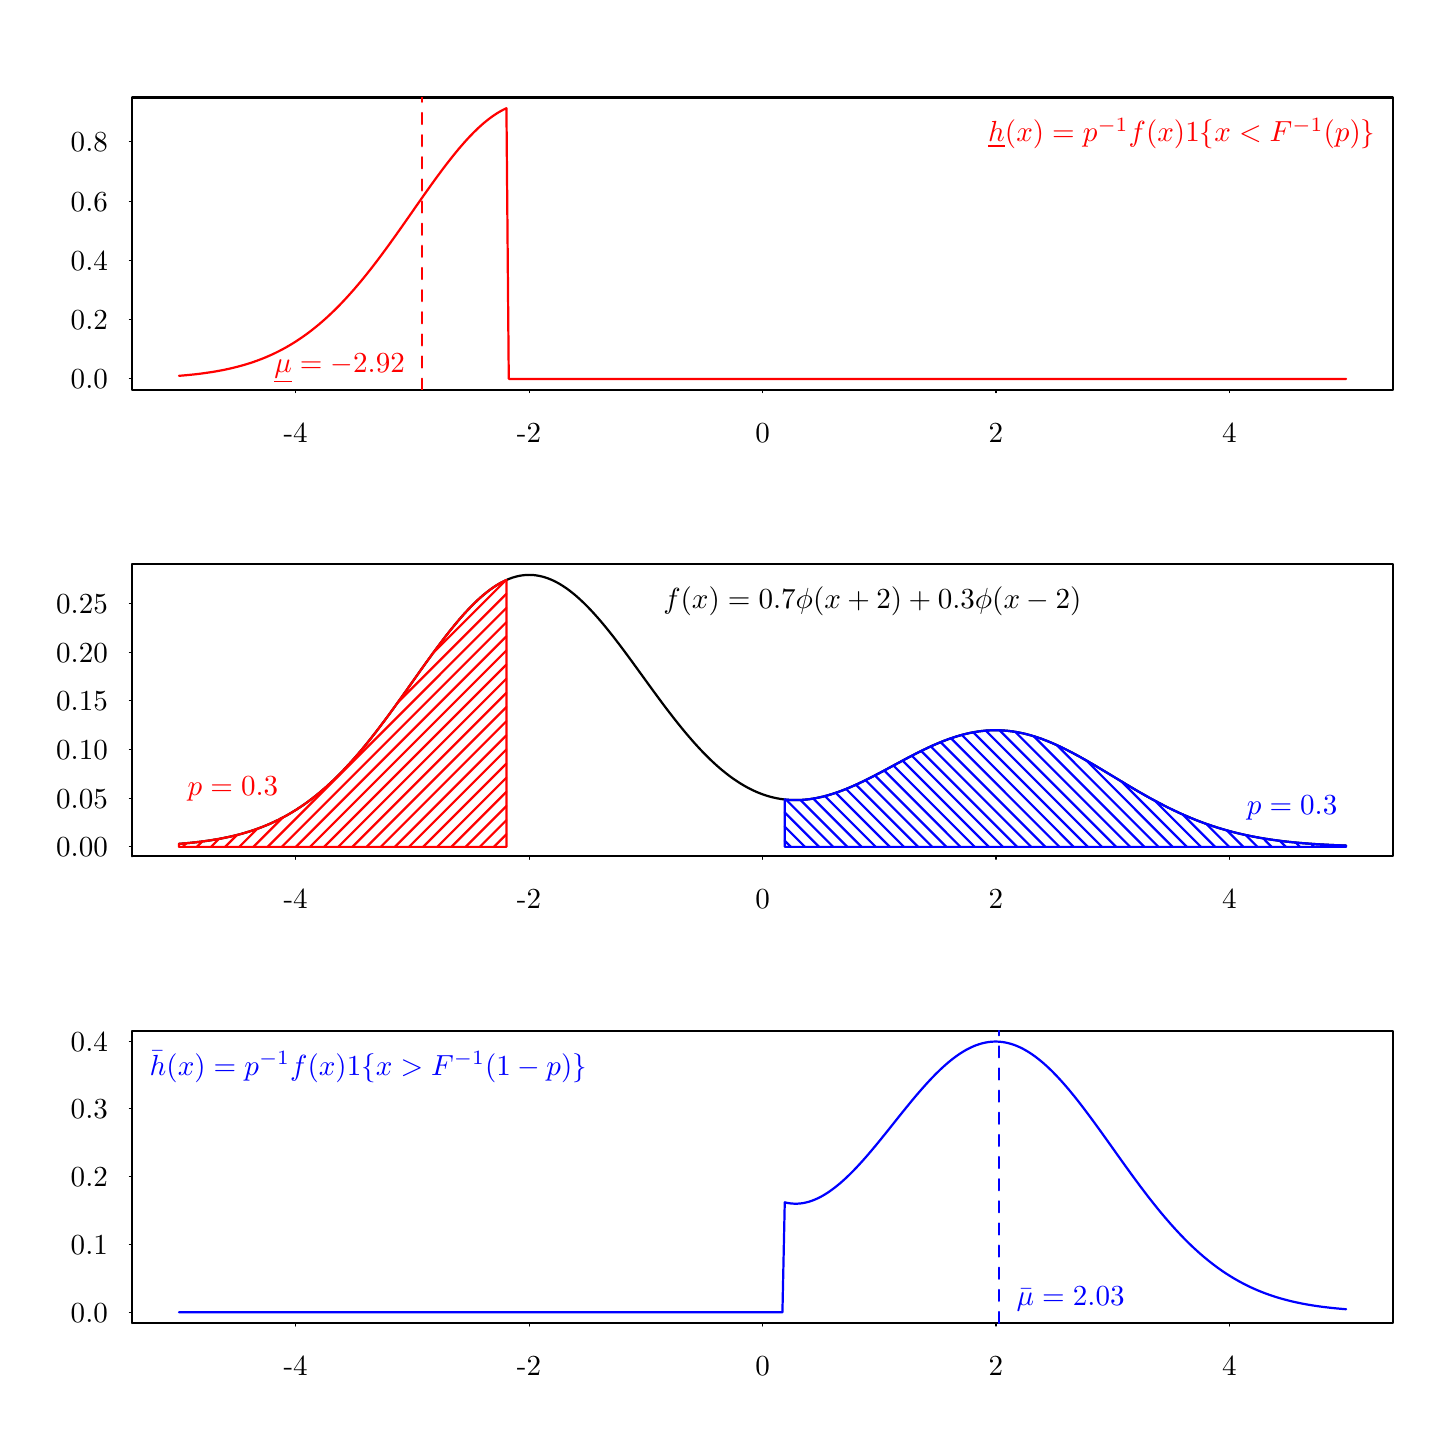
\begin{tikzpicture}[x=1pt,y=1pt]
\definecolor{fillColor}{RGB}{255,255,255}
\path[use as bounding box,fill=fillColor,fill opacity=0.00] (0,0) rectangle (505.89,505.89);
\begin{scope}
\path[clip] ( 37.80,375.06) rectangle (493.29,480.69);
\definecolor{drawColor}{RGB}{255,0,0}

\path[draw=drawColor,line width= 0.8pt,line join=round,line cap=round] ( 54.67,380.08) --
	( 55.52,380.15) --
	( 56.36,380.22) --
	( 57.21,380.30) --
	( 58.05,380.38) --
	( 58.90,380.46) --
	( 59.74,380.55) --
	( 60.59,380.64) --
	( 61.43,380.74) --
	( 62.28,380.84) --
	( 63.12,380.95) --
	( 63.97,381.07) --
	( 64.81,381.19) --
	( 65.66,381.31) --
	( 66.50,381.44) --
	( 67.35,381.58) --
	( 68.19,381.72) --
	( 69.04,381.88) --
	( 69.88,382.03) --
	( 70.73,382.20) --
	( 71.57,382.37) --
	( 72.42,382.55) --
	( 73.26,382.74) --
	( 74.11,382.94) --
	( 74.95,383.15) --
	( 75.80,383.36) --
	( 76.64,383.59) --
	( 77.49,383.82) --
	( 78.34,384.06) --
	( 79.18,384.32) --
	( 80.03,384.58) --
	( 80.87,384.86) --
	( 81.72,385.14) --
	( 82.56,385.44) --
	( 83.41,385.75) --
	( 84.25,386.07) --
	( 85.10,386.40) --
	( 85.94,386.75) --
	( 86.79,387.11) --
	( 87.63,387.48) --
	( 88.48,387.87) --
	( 89.32,388.26) --
	( 90.17,388.68) --
	( 91.01,389.10) --
	( 91.86,389.55) --
	( 92.70,390.00) --
	( 93.55,390.47) --
	( 94.39,390.96) --
	( 95.24,391.46) --
	( 96.08,391.98) --
	( 96.93,392.51) --
	( 97.77,393.06) --
	( 98.62,393.63) --
	( 99.47,394.22) --
	(100.31,394.82) --
	(101.16,395.43) --
	(102.00,396.07) --
	(102.85,396.72) --
	(103.69,397.39) --
	(104.54,398.08) --
	(105.38,398.78) --
	(106.23,399.50) --
	(107.07,400.24) --
	(107.92,401.00) --
	(108.76,401.78) --
	(109.61,402.57) --
	(110.45,403.38) --
	(111.30,404.21) --
	(112.14,405.06) --
	(112.99,405.92) --
	(113.83,406.81) --
	(114.68,407.71) --
	(115.52,408.62) --
	(116.37,409.56) --
	(117.21,410.51) --
	(118.06,411.47) --
	(118.90,412.46) --
	(119.75,413.46) --
	(120.59,414.47) --
	(121.44,415.50) --
	(122.29,416.55) --
	(123.13,417.60) --
	(123.98,418.68) --
	(124.82,419.76) --
	(125.67,420.86) --
	(126.51,421.97) --
	(127.36,423.10) --
	(128.20,424.23) --
	(129.05,425.38) --
	(129.89,426.53) --
	(130.74,427.69) --
	(131.58,428.87) --
	(132.43,430.05) --
	(133.27,431.23) --
	(134.12,432.43) --
	(134.96,433.62) --
	(135.81,434.83) --
	(136.65,436.03) --
	(137.50,437.24) --
	(138.34,438.45) --
	(139.19,439.66) --
	(140.03,440.88) --
	(140.88,442.09) --
	(141.72,443.29) --
	(142.57,444.50) --
	(143.41,445.70) --
	(144.26,446.89) --
	(145.11,448.08) --
	(145.95,449.26) --
	(146.80,450.44) --
	(147.64,451.60) --
	(148.49,452.75) --
	(149.33,453.89) --
	(150.18,455.02) --
	(151.02,456.13) --
	(151.87,457.23) --
	(152.71,458.31) --
	(153.56,459.38) --
	(154.40,460.43) --
	(155.25,461.45) --
	(156.09,462.46) --
	(156.94,463.44) --
	(157.78,464.41) --
	(158.63,465.35) --
	(159.47,466.26) --
	(160.32,467.15) --
	(161.16,468.01) --
	(162.01,468.84) --
	(162.85,469.65) --
	(163.70,470.42) --
	(164.54,471.17) --
	(165.39,471.88) --
	(166.24,472.56) --
	(167.08,473.21) --
	(167.93,473.83) --
	(168.77,474.41) --
	(169.62,474.95) --
	(170.46,475.47) --
	(171.31,475.94) --
	(172.15,476.38) --
	(173.00,476.78) --
	(173.84,378.97) --
	(174.69,378.97) --
	(175.53,378.97) --
	(176.38,378.97) --
	(177.22,378.97) --
	(178.07,378.97) --
	(178.91,378.97) --
	(179.76,378.97) --
	(180.60,378.97) --
	(181.45,378.97) --
	(182.29,378.97) --
	(183.14,378.97) --
	(183.98,378.97) --
	(184.83,378.97) --
	(185.67,378.97) --
	(186.52,378.97) --
	(187.36,378.97) --
	(188.21,378.97) --
	(189.06,378.97) --
	(189.90,378.97) --
	(190.75,378.97) --
	(191.59,378.97) --
	(192.44,378.97) --
	(193.28,378.97) --
	(194.13,378.97) --
	(194.97,378.97) --
	(195.82,378.97) --
	(196.66,378.97) --
	(197.51,378.97) --
	(198.35,378.97) --
	(199.20,378.97) --
	(200.04,378.97) --
	(200.89,378.97) --
	(201.73,378.97) --
	(202.58,378.97) --
	(203.42,378.97) --
	(204.27,378.97) --
	(205.11,378.97) --
	(205.96,378.97) --
	(206.80,378.97) --
	(207.65,378.97) --
	(208.49,378.97) --
	(209.34,378.97) --
	(210.19,378.97) --
	(211.03,378.97) --
	(211.88,378.97) --
	(212.72,378.97) --
	(213.57,378.97) --
	(214.41,378.97) --
	(215.26,378.97) --
	(216.10,378.97) --
	(216.95,378.97) --
	(217.79,378.97) --
	(218.64,378.97) --
	(219.48,378.97) --
	(220.33,378.97) --
	(221.17,378.97) --
	(222.02,378.97) --
	(222.86,378.97) --
	(223.71,378.97) --
	(224.55,378.97) --
	(225.40,378.97) --
	(226.24,378.97) --
	(227.09,378.97) --
	(227.93,378.97) --
	(228.78,378.97) --
	(229.62,378.97) --
	(230.47,378.97) --
	(231.31,378.97) --
	(232.16,378.97) --
	(233.01,378.97) --
	(233.85,378.97) --
	(234.70,378.97) --
	(235.54,378.97) --
	(236.39,378.97) --
	(237.23,378.97) --
	(238.08,378.97) --
	(238.92,378.97) --
	(239.77,378.97) --
	(240.61,378.97) --
	(241.46,378.97) --
	(242.30,378.97) --
	(243.15,378.97) --
	(243.99,378.97) --
	(244.84,378.97) --
	(245.68,378.97) --
	(246.53,378.97) --
	(247.37,378.97) --
	(248.22,378.97) --
	(249.06,378.97) --
	(249.91,378.97) --
	(250.75,378.97) --
	(251.60,378.97) --
	(252.44,378.97) --
	(253.29,378.97) --
	(254.13,378.97) --
	(254.98,378.97) --
	(255.83,378.97) --
	(256.67,378.97) --
	(257.52,378.97) --
	(258.36,378.97) --
	(259.21,378.97) --
	(260.05,378.97) --
	(260.90,378.97) --
	(261.74,378.97) --
	(262.59,378.97) --
	(263.43,378.97) --
	(264.28,378.97) --
	(265.12,378.97) --
	(265.97,378.97) --
	(266.81,378.97) --
	(267.66,378.97) --
	(268.50,378.97) --
	(269.35,378.97) --
	(270.19,378.97) --
	(271.04,378.97) --
	(271.88,378.97) --
	(272.73,378.97) --
	(273.57,378.97) --
	(274.42,378.97) --
	(275.26,378.97) --
	(276.11,378.97) --
	(276.96,378.97) --
	(277.80,378.97) --
	(278.65,378.97) --
	(279.49,378.97) --
	(280.34,378.97) --
	(281.18,378.97) --
	(282.03,378.97) --
	(282.87,378.97) --
	(283.72,378.97) --
	(284.56,378.97) --
	(285.41,378.97) --
	(286.25,378.97) --
	(287.10,378.97) --
	(287.94,378.97) --
	(288.79,378.97) --
	(289.63,378.97) --
	(290.48,378.97) --
	(291.32,378.97) --
	(292.17,378.97) --
	(293.01,378.97) --
	(293.86,378.97) --
	(294.70,378.97) --
	(295.55,378.97) --
	(296.39,378.97) --
	(297.24,378.97) --
	(298.08,378.97) --
	(298.93,378.97) --
	(299.78,378.97) --
	(300.62,378.97) --
	(301.47,378.97) --
	(302.31,378.97) --
	(303.16,378.97) --
	(304.00,378.97) --
	(304.85,378.97) --
	(305.69,378.97) --
	(306.54,378.97) --
	(307.38,378.97) --
	(308.23,378.97) --
	(309.07,378.97) --
	(309.92,378.97) --
	(310.76,378.97) --
	(311.61,378.97) --
	(312.45,378.97) --
	(313.30,378.97) --
	(314.14,378.97) --
	(314.99,378.97) --
	(315.83,378.97) --
	(316.68,378.97) --
	(317.52,378.97) --
	(318.37,378.97) --
	(319.21,378.97) --
	(320.06,378.97) --
	(320.90,378.97) --
	(321.75,378.97) --
	(322.60,378.97) --
	(323.44,378.97) --
	(324.29,378.97) --
	(325.13,378.97) --
	(325.98,378.97) --
	(326.82,378.97) --
	(327.67,378.97) --
	(328.51,378.97) --
	(329.36,378.97) --
	(330.20,378.97) --
	(331.05,378.97) --
	(331.89,378.97) --
	(332.74,378.97) --
	(333.58,378.97) --
	(334.43,378.97) --
	(335.27,378.97) --
	(336.12,378.97) --
	(336.96,378.97) --
	(337.81,378.97) --
	(338.65,378.97) --
	(339.50,378.97) --
	(340.34,378.97) --
	(341.19,378.97) --
	(342.03,378.97) --
	(342.88,378.97) --
	(343.73,378.97) --
	(344.57,378.97) --
	(345.42,378.97) --
	(346.26,378.97) --
	(347.11,378.97) --
	(347.95,378.97) --
	(348.80,378.97) --
	(349.64,378.97) --
	(350.49,378.97) --
	(351.33,378.97) --
	(352.18,378.97) --
	(353.02,378.97) --
	(353.87,378.97) --
	(354.71,378.97) --
	(355.56,378.97) --
	(356.40,378.97) --
	(357.25,378.97) --
	(358.09,378.97) --
	(358.94,378.97) --
	(359.78,378.97) --
	(360.63,378.97) --
	(361.47,378.97) --
	(362.32,378.97) --
	(363.16,378.97) --
	(364.01,378.97) --
	(364.85,378.97) --
	(365.70,378.97) --
	(366.55,378.97) --
	(367.39,378.97) --
	(368.24,378.97) --
	(369.08,378.97) --
	(369.93,378.97) --
	(370.77,378.97) --
	(371.62,378.97) --
	(372.46,378.97) --
	(373.31,378.97) --
	(374.15,378.97) --
	(375.00,378.97) --
	(375.84,378.97) --
	(376.69,378.97) --
	(377.53,378.97) --
	(378.38,378.97) --
	(379.22,378.97) --
	(380.07,378.97) --
	(380.91,378.97) --
	(381.76,378.97) --
	(382.60,378.97) --
	(383.45,378.97) --
	(384.29,378.97) --
	(385.14,378.97) --
	(385.98,378.97) --
	(386.83,378.97) --
	(387.68,378.97) --
	(388.52,378.97) --
	(389.37,378.97) --
	(390.21,378.97) --
	(391.06,378.97) --
	(391.90,378.97) --
	(392.75,378.97) --
	(393.59,378.97) --
	(394.44,378.97) --
	(395.28,378.97) --
	(396.13,378.97) --
	(396.97,378.97) --
	(397.82,378.97) --
	(398.66,378.97) --
	(399.51,378.97) --
	(400.35,378.97) --
	(401.20,378.97) --
	(402.04,378.97) --
	(402.89,378.97) --
	(403.73,378.97) --
	(404.58,378.97) --
	(405.42,378.97) --
	(406.27,378.97) --
	(407.11,378.97) --
	(407.96,378.97) --
	(408.80,378.97) --
	(409.65,378.97) --
	(410.50,378.97) --
	(411.34,378.97) --
	(412.19,378.97) --
	(413.03,378.97) --
	(413.88,378.97) --
	(414.72,378.97) --
	(415.57,378.97) --
	(416.41,378.97) --
	(417.26,378.97) --
	(418.10,378.97) --
	(418.95,378.97) --
	(419.79,378.97) --
	(420.64,378.97) --
	(421.48,378.97) --
	(422.33,378.97) --
	(423.17,378.97) --
	(424.02,378.97) --
	(424.86,378.97) --
	(425.71,378.97) --
	(426.55,378.97) --
	(427.40,378.97) --
	(428.24,378.97) --
	(429.09,378.97) --
	(429.93,378.97) --
	(430.78,378.97) --
	(431.62,378.97) --
	(432.47,378.97) --
	(433.32,378.97) --
	(434.16,378.97) --
	(435.01,378.97) --
	(435.85,378.97) --
	(436.70,378.97) --
	(437.54,378.97) --
	(438.39,378.97) --
	(439.23,378.97) --
	(440.08,378.97) --
	(440.92,378.97) --
	(441.77,378.97) --
	(442.61,378.97) --
	(443.46,378.97) --
	(444.30,378.97) --
	(445.15,378.97) --
	(445.99,378.97) --
	(446.84,378.97) --
	(447.68,378.97) --
	(448.53,378.97) --
	(449.37,378.97) --
	(450.22,378.97) --
	(451.06,378.97) --
	(451.91,378.97) --
	(452.75,378.97) --
	(453.60,378.97) --
	(454.45,378.97) --
	(455.29,378.97) --
	(456.14,378.97) --
	(456.98,378.97) --
	(457.83,378.97) --
	(458.67,378.97) --
	(459.52,378.97) --
	(460.36,378.97) --
	(461.21,378.97) --
	(462.05,378.97) --
	(462.90,378.97) --
	(463.74,378.97) --
	(464.59,378.97) --
	(465.43,378.97) --
	(466.28,378.97) --
	(467.12,378.97) --
	(467.97,378.97) --
	(468.81,378.97) --
	(469.66,378.97) --
	(470.50,378.97) --
	(471.35,378.97) --
	(472.19,378.97) --
	(473.04,378.97) --
	(473.88,378.97) --
	(474.73,378.97) --
	(475.57,378.97) --
	(476.42,378.97);
\end{scope}
\begin{scope}
\path[clip] (  0.00,  0.00) rectangle (505.89,505.89);
\definecolor{drawColor}{RGB}{0,0,0}

\path[draw=drawColor,line width= 0.4pt,line join=round,line cap=round] ( 96.84,375.06) -- (434.25,375.06);

\path[draw=drawColor,line width= 0.4pt,line join=round,line cap=round] ( 96.84,375.06) -- ( 96.84,374.00);

\path[draw=drawColor,line width= 0.4pt,line join=round,line cap=round] (181.19,375.06) -- (181.19,374.00);

\path[draw=drawColor,line width= 0.4pt,line join=round,line cap=round] (265.54,375.06) -- (265.54,374.00);

\path[draw=drawColor,line width= 0.4pt,line join=round,line cap=round] (349.89,375.06) -- (349.89,374.00);

\path[draw=drawColor,line width= 0.4pt,line join=round,line cap=round] (434.25,375.06) -- (434.25,374.00);

\node[text=drawColor,anchor=base,inner sep=0pt, outer sep=0pt, scale=  1.05] at ( 96.84,356.16) {-4};

\node[text=drawColor,anchor=base,inner sep=0pt, outer sep=0pt, scale=  1.05] at (181.19,356.16) {-2};

\node[text=drawColor,anchor=base,inner sep=0pt, outer sep=0pt, scale=  1.05] at (265.54,356.16) {0};

\node[text=drawColor,anchor=base,inner sep=0pt, outer sep=0pt, scale=  1.05] at (349.89,356.16) {2};

\node[text=drawColor,anchor=base,inner sep=0pt, outer sep=0pt, scale=  1.05] at (434.25,356.16) {4};

\path[draw=drawColor,line width= 0.4pt,line join=round,line cap=round] ( 37.80,378.97) -- ( 37.80,464.63);

\path[draw=drawColor,line width= 0.4pt,line join=round,line cap=round] ( 37.80,378.97) -- ( 36.74,378.97);

\path[draw=drawColor,line width= 0.4pt,line join=round,line cap=round] ( 37.80,400.39) -- ( 36.74,400.39);

\path[draw=drawColor,line width= 0.4pt,line join=round,line cap=round] ( 37.80,421.80) -- ( 36.74,421.80);

\path[draw=drawColor,line width= 0.4pt,line join=round,line cap=round] ( 37.80,443.21) -- ( 36.74,443.21);

\path[draw=drawColor,line width= 0.4pt,line join=round,line cap=round] ( 37.80,464.63) -- ( 36.74,464.63);

\node[text=drawColor,anchor=base east,inner sep=0pt, outer sep=0pt, scale=  1.05] at ( 28.98,375.36) {0.0};

\node[text=drawColor,anchor=base east,inner sep=0pt, outer sep=0pt, scale=  1.05] at ( 28.98,396.77) {0.2};

\node[text=drawColor,anchor=base east,inner sep=0pt, outer sep=0pt, scale=  1.05] at ( 28.98,418.18) {0.4};

\node[text=drawColor,anchor=base east,inner sep=0pt, outer sep=0pt, scale=  1.05] at ( 28.98,439.60) {0.6};

\node[text=drawColor,anchor=base east,inner sep=0pt, outer sep=0pt, scale=  1.05] at ( 28.98,461.01) {0.8};

\path[draw=drawColor,line width= 0.8pt,line join=round,line cap=round] ( 37.80,375.06) --
	(493.29,375.06) --
	(493.29,480.69) --
	( 37.80,480.69) --
	( 37.80,375.06);
\end{scope}
\begin{scope}
\path[clip] ( 37.80,375.06) rectangle (493.29,480.69);
\definecolor{drawColor}{RGB}{255,0,0}

\node[text=drawColor,anchor=base east,inner sep=0pt, outer sep=0pt, scale=  1.05] at (486.99,464.59) {$\underline{h}(x) = p^{-1}f(x) 1\{x < F^{-1}(p)\}$};

\path[draw=drawColor,line width= 0.8pt,dash pattern=on 4pt off 4pt ,line join=round,line cap=round] (142.60,375.06) -- (142.60,480.69);

\node[text=drawColor,anchor=base east,inner sep=0pt, outer sep=0pt, scale=  1.05] at (136.30,381.45) {$\underline{\mu} = -2.92$};
\end{scope}
\begin{scope}
\path[clip] ( 37.80,206.43) rectangle (493.29,312.06);
\definecolor{drawColor}{RGB}{0,0,0}

\path[draw=drawColor,line width= 0.8pt,line join=round,line cap=round] ( 54.67,210.97) --
	( 55.52,211.03) --
	( 56.36,211.10) --
	( 57.21,211.18) --
	( 58.05,211.26) --
	( 58.90,211.34) --
	( 59.74,211.43) --
	( 60.59,211.52) --
	( 61.43,211.62) --
	( 62.28,211.72) --
	( 63.12,211.83) --
	( 63.97,211.94) --
	( 64.81,212.06) --
	( 65.66,212.18) --
	( 66.50,212.31) --
	( 67.35,212.45) --
	( 68.19,212.59) --
	( 69.04,212.74) --
	( 69.88,212.89) --
	( 70.73,213.06) --
	( 71.57,213.23) --
	( 72.42,213.41) --
	( 73.26,213.59) --
	( 74.11,213.79) --
	( 74.95,213.99) --
	( 75.80,214.20) --
	( 76.64,214.42) --
	( 77.49,214.65) --
	( 78.34,214.90) --
	( 79.18,215.15) --
	( 80.03,215.41) --
	( 80.87,215.68) --
	( 81.72,215.96) --
	( 82.56,216.25) --
	( 83.41,216.56) --
	( 84.25,216.87) --
	( 85.10,217.20) --
	( 85.94,217.54) --
	( 86.79,217.90) --
	( 87.63,218.26) --
	( 88.48,218.64) --
	( 89.32,219.04) --
	( 90.17,219.44) --
	( 91.01,219.86) --
	( 91.86,220.30) --
	( 92.70,220.75) --
	( 93.55,221.21) --
	( 94.39,221.69) --
	( 95.24,222.19) --
	( 96.08,222.70) --
	( 96.93,223.23) --
	( 97.77,223.77) --
	( 98.62,224.33) --
	( 99.47,224.90) --
	(100.31,225.49) --
	(101.16,226.10) --
	(102.00,226.73) --
	(102.85,227.37) --
	(103.69,228.03) --
	(104.54,228.71) --
	(105.38,229.40) --
	(106.23,230.12) --
	(107.07,230.85) --
	(107.92,231.59) --
	(108.76,232.36) --
	(109.61,233.14) --
	(110.45,233.94) --
	(111.30,234.76) --
	(112.14,235.59) --
	(112.99,236.45) --
	(113.83,237.32) --
	(114.68,238.20) --
	(115.52,239.11) --
	(116.37,240.03) --
	(117.21,240.97) --
	(118.06,241.92) --
	(118.90,242.89) --
	(119.75,243.87) --
	(120.59,244.87) --
	(121.44,245.89) --
	(122.29,246.92) --
	(123.13,247.96) --
	(123.98,249.02) --
	(124.82,250.09) --
	(125.67,251.17) --
	(126.51,252.27) --
	(127.36,253.38) --
	(128.20,254.50) --
	(129.05,255.62) --
	(129.89,256.76) --
	(130.74,257.91) --
	(131.58,259.07) --
	(132.43,260.23) --
	(133.27,261.40) --
	(134.12,262.58) --
	(134.96,263.76) --
	(135.81,264.94) --
	(136.65,266.13) --
	(137.50,267.32) --
	(138.34,268.52) --
	(139.19,269.71) --
	(140.03,270.91) --
	(140.88,272.10) --
	(141.72,273.29) --
	(142.57,274.48) --
	(143.41,275.66) --
	(144.26,276.84) --
	(145.11,278.01) --
	(145.95,279.18) --
	(146.80,280.33) --
	(147.64,281.48) --
	(148.49,282.61) --
	(149.33,283.74) --
	(150.18,284.85) --
	(151.02,285.95) --
	(151.87,287.03) --
	(152.71,288.10) --
	(153.56,289.15) --
	(154.40,290.18) --
	(155.25,291.19) --
	(156.09,292.19) --
	(156.94,293.16) --
	(157.78,294.11) --
	(158.63,295.03) --
	(159.47,295.93) --
	(160.32,296.81) --
	(161.16,297.66) --
	(162.01,298.48) --
	(162.85,299.27) --
	(163.70,300.04) --
	(164.54,300.77) --
	(165.39,301.47) --
	(166.24,302.15) --
	(167.08,302.79) --
	(167.93,303.39) --
	(168.77,303.97) --
	(169.62,304.51) --
	(170.46,305.01) --
	(171.31,305.48) --
	(172.15,305.91) --
	(173.00,306.30) --
	(173.84,306.66) --
	(174.69,306.98) --
	(175.53,307.26) --
	(176.38,307.50) --
	(177.22,307.71) --
	(178.07,307.88) --
	(178.91,308.00) --
	(179.76,308.09) --
	(180.60,308.14) --
	(181.45,308.15) --
	(182.29,308.12) --
	(183.14,308.05) --
	(183.98,307.94) --
	(184.83,307.79) --
	(185.67,307.60) --
	(186.52,307.38) --
	(187.36,307.11) --
	(188.21,306.81) --
	(189.06,306.47) --
	(189.90,306.10) --
	(190.75,305.68) --
	(191.59,305.23) --
	(192.44,304.75) --
	(193.28,304.22) --
	(194.13,303.67) --
	(194.97,303.08) --
	(195.82,302.46) --
	(196.66,301.80) --
	(197.51,301.12) --
	(198.35,300.40) --
	(199.20,299.65) --
	(200.04,298.87) --
	(200.89,298.07) --
	(201.73,297.24) --
	(202.58,296.38) --
	(203.42,295.49) --
	(204.27,294.59) --
	(205.11,293.65) --
	(205.96,292.70) --
	(206.80,291.73) --
	(207.65,290.73) --
	(208.49,289.72) --
	(209.34,288.68) --
	(210.19,287.63) --
	(211.03,286.57) --
	(211.88,285.49) --
	(212.72,284.40) --
	(213.57,283.29) --
	(214.41,282.18) --
	(215.26,281.05) --
	(216.10,279.91) --
	(216.95,278.77) --
	(217.79,277.62) --
	(218.64,276.46) --
	(219.48,275.30) --
	(220.33,274.14) --
	(221.17,272.97) --
	(222.02,271.81) --
	(222.86,270.64) --
	(223.71,269.47) --
	(224.55,268.31) --
	(225.40,267.15) --
	(226.24,265.99) --
	(227.09,264.84) --
	(227.93,263.69) --
	(228.78,262.55) --
	(229.62,261.42) --
	(230.47,260.29) --
	(231.31,259.18) --
	(232.16,258.08) --
	(233.01,256.98) --
	(233.85,255.90) --
	(234.70,254.83) --
	(235.54,253.78) --
	(236.39,252.74) --
	(237.23,251.71) --
	(238.08,250.70) --
	(238.92,249.71) --
	(239.77,248.73) --
	(240.61,247.77) --
	(241.46,246.82) --
	(242.30,245.90) --
	(243.15,244.99) --
	(243.99,244.10) --
	(244.84,243.24) --
	(245.68,242.39) --
	(246.53,241.56) --
	(247.37,240.76) --
	(248.22,239.97) --
	(249.06,239.21) --
	(249.91,238.47) --
	(250.75,237.75) --
	(251.60,237.05) --
	(252.44,236.38) --
	(253.29,235.73) --
	(254.13,235.10) --
	(254.98,234.49) --
	(255.83,233.91) --
	(256.67,233.35) --
	(257.52,232.81) --
	(258.36,232.30) --
	(259.21,231.81) --
	(260.05,231.34) --
	(260.90,230.90) --
	(261.74,230.48) --
	(262.59,230.08) --
	(263.43,229.70) --
	(264.28,229.35) --
	(265.12,229.03) --
	(265.97,228.72) --
	(266.81,228.44) --
	(267.66,228.18) --
	(268.50,227.94) --
	(269.35,227.73) --
	(270.19,227.54) --
	(271.04,227.37) --
	(271.88,227.22) --
	(272.73,227.09) --
	(273.57,226.99) --
	(274.42,226.90) --
	(275.26,226.84) --
	(276.11,226.80) --
	(276.96,226.78) --
	(277.80,226.77) --
	(278.65,226.79) --
	(279.49,226.83) --
	(280.34,226.88) --
	(281.18,226.96) --
	(282.03,227.05) --
	(282.87,227.16) --
	(283.72,227.29) --
	(284.56,227.44) --
	(285.41,227.60) --
	(286.25,227.78) --
	(287.10,227.97) --
	(287.94,228.18) --
	(288.79,228.41) --
	(289.63,228.65) --
	(290.48,228.91) --
	(291.32,229.18) --
	(292.17,229.46) --
	(293.01,229.76) --
	(293.86,230.07) --
	(294.70,230.39) --
	(295.55,230.72) --
	(296.39,231.07) --
	(297.24,231.42) --
	(298.08,231.79) --
	(298.93,232.16) --
	(299.78,232.55) --
	(300.62,232.94) --
	(301.47,233.34) --
	(302.31,233.75) --
	(303.16,234.16) --
	(304.00,234.59) --
	(304.85,235.01) --
	(305.69,235.45) --
	(306.54,235.89) --
	(307.38,236.33) --
	(308.23,236.78) --
	(309.07,237.23) --
	(309.92,237.68) --
	(310.76,238.13) --
	(311.61,238.59) --
	(312.45,239.05) --
	(313.30,239.50) --
	(314.14,239.96) --
	(314.99,240.41) --
	(315.83,240.87) --
	(316.68,241.32) --
	(317.52,241.77) --
	(318.37,242.22) --
	(319.21,242.66) --
	(320.06,243.10) --
	(320.90,243.53) --
	(321.75,243.96) --
	(322.60,244.38) --
	(323.44,244.80) --
	(324.29,245.21) --
	(325.13,245.61) --
	(325.98,246.00) --
	(326.82,246.39) --
	(327.67,246.76) --
	(328.51,247.13) --
	(329.36,247.48) --
	(330.20,247.83) --
	(331.05,248.16) --
	(331.89,248.49) --
	(332.74,248.80) --
	(333.58,249.09) --
	(334.43,249.38) --
	(335.27,249.65) --
	(336.12,249.91) --
	(336.96,250.16) --
	(337.81,250.39) --
	(338.65,250.61) --
	(339.50,250.81) --
	(340.34,251.00) --
	(341.19,251.17) --
	(342.03,251.33) --
	(342.88,251.47) --
	(343.73,251.60) --
	(344.57,251.71) --
	(345.42,251.80) --
	(346.26,251.88) --
	(347.11,251.94) --
	(347.95,251.98) --
	(348.80,252.01) --
	(349.64,252.02) --
	(350.49,252.01) --
	(351.33,251.99) --
	(352.18,251.95) --
	(353.02,251.89) --
	(353.87,251.82) --
	(354.71,251.73) --
	(355.56,251.63) --
	(356.40,251.51) --
	(357.25,251.37) --
	(358.09,251.21) --
	(358.94,251.04) --
	(359.78,250.86) --
	(360.63,250.66) --
	(361.47,250.44) --
	(362.32,250.21) --
	(363.16,249.96) --
	(364.01,249.70) --
	(364.85,249.43) --
	(365.70,249.14) --
	(366.55,248.84) --
	(367.39,248.52) --
	(368.24,248.19) --
	(369.08,247.85) --
	(369.93,247.50) --
	(370.77,247.13) --
	(371.62,246.76) --
	(372.46,246.37) --
	(373.31,245.98) --
	(374.15,245.57) --
	(375.00,245.15) --
	(375.84,244.73) --
	(376.69,244.29) --
	(377.53,243.85) --
	(378.38,243.40) --
	(379.22,242.94) --
	(380.07,242.48) --
	(380.91,242.01) --
	(381.76,241.53) --
	(382.60,241.05) --
	(383.45,240.56) --
	(384.29,240.07) --
	(385.14,239.58) --
	(385.98,239.08) --
	(386.83,238.57) --
	(387.68,238.07) --
	(388.52,237.56) --
	(389.37,237.05) --
	(390.21,236.54) --
	(391.06,236.03) --
	(391.90,235.52) --
	(392.75,235.01) --
	(393.59,234.50) --
	(394.44,233.98) --
	(395.28,233.48) --
	(396.13,232.97) --
	(396.97,232.46) --
	(397.82,231.96) --
	(398.66,231.46) --
	(399.51,230.96) --
	(400.35,230.46) --
	(401.20,229.97) --
	(402.04,229.48) --
	(402.89,229.00) --
	(403.73,228.52) --
	(404.58,228.04) --
	(405.42,227.57) --
	(406.27,227.11) --
	(407.11,226.65) --
	(407.96,226.20) --
	(408.80,225.75) --
	(409.65,225.31) --
	(410.50,224.87) --
	(411.34,224.45) --
	(412.19,224.02) --
	(413.03,223.61) --
	(413.88,223.20) --
	(414.72,222.80) --
	(415.57,222.40) --
	(416.41,222.02) --
	(417.26,221.64) --
	(418.10,221.26) --
	(418.95,220.90) --
	(419.79,220.54) --
	(420.64,220.19) --
	(421.48,219.85) --
	(422.33,219.51) --
	(423.17,219.18) --
	(424.02,218.86) --
	(424.86,218.55) --
	(425.71,218.24) --
	(426.55,217.95) --
	(427.40,217.66) --
	(428.24,217.37) --
	(429.09,217.10) --
	(429.93,216.83) --
	(430.78,216.57) --
	(431.62,216.32) --
	(432.47,216.07) --
	(433.32,215.83) --
	(434.16,215.60) --
	(435.01,215.37) --
	(435.85,215.15) --
	(436.70,214.94) --
	(437.54,214.73) --
	(438.39,214.53) --
	(439.23,214.34) --
	(440.08,214.16) --
	(440.92,213.98) --
	(441.77,213.80) --
	(442.61,213.63) --
	(443.46,213.47) --
	(444.30,213.31) --
	(445.15,213.16) --
	(445.99,213.02) --
	(446.84,212.87) --
	(447.68,212.74) --
	(448.53,212.61) --
	(449.37,212.48) --
	(450.22,212.36) --
	(451.06,212.25) --
	(451.91,212.13) --
	(452.75,212.03) --
	(453.60,211.92) --
	(454.45,211.82) --
	(455.29,211.73) --
	(456.14,211.64) --
	(456.98,211.55) --
	(457.83,211.47) --
	(458.67,211.39) --
	(459.52,211.31) --
	(460.36,211.24) --
	(461.21,211.17) --
	(462.05,211.10) --
	(462.90,211.04) --
	(463.74,210.98) --
	(464.59,210.92) --
	(465.43,210.86) --
	(466.28,210.81) --
	(467.12,210.76) --
	(467.97,210.71) --
	(468.81,210.67) --
	(469.66,210.62) --
	(470.50,210.58) --
	(471.35,210.54) --
	(472.19,210.50) --
	(473.04,210.47) --
	(473.88,210.43) --
	(474.73,210.40) --
	(475.57,210.37) --
	(476.42,210.34);
\end{scope}
\begin{scope}
\path[clip] (  0.00,  0.00) rectangle (505.89,505.89);
\definecolor{drawColor}{RGB}{0,0,0}

\path[draw=drawColor,line width= 0.4pt,line join=round,line cap=round] ( 96.84,206.43) -- (434.25,206.43);

\path[draw=drawColor,line width= 0.4pt,line join=round,line cap=round] ( 96.84,206.43) -- ( 96.84,205.37);

\path[draw=drawColor,line width= 0.4pt,line join=round,line cap=round] (181.19,206.43) -- (181.19,205.37);

\path[draw=drawColor,line width= 0.4pt,line join=round,line cap=round] (265.54,206.43) -- (265.54,205.37);

\path[draw=drawColor,line width= 0.4pt,line join=round,line cap=round] (349.89,206.43) -- (349.89,205.37);

\path[draw=drawColor,line width= 0.4pt,line join=round,line cap=round] (434.25,206.43) -- (434.25,205.37);

\node[text=drawColor,anchor=base,inner sep=0pt, outer sep=0pt, scale=  1.05] at ( 96.84,187.53) {-4};

\node[text=drawColor,anchor=base,inner sep=0pt, outer sep=0pt, scale=  1.05] at (181.19,187.53) {-2};

\node[text=drawColor,anchor=base,inner sep=0pt, outer sep=0pt, scale=  1.05] at (265.54,187.53) {0};

\node[text=drawColor,anchor=base,inner sep=0pt, outer sep=0pt, scale=  1.05] at (349.89,187.53) {2};

\node[text=drawColor,anchor=base,inner sep=0pt, outer sep=0pt, scale=  1.05] at (434.25,187.53) {4};

\path[draw=drawColor,line width= 0.4pt,line join=round,line cap=round] ( 37.80,209.87) -- ( 37.80,297.84);

\path[draw=drawColor,line width= 0.4pt,line join=round,line cap=round] ( 37.80,209.87) -- ( 36.74,209.87);

\path[draw=drawColor,line width= 0.4pt,line join=round,line cap=round] ( 37.80,227.47) -- ( 36.74,227.47);

\path[draw=drawColor,line width= 0.4pt,line join=round,line cap=round] ( 37.80,245.06) -- ( 36.74,245.06);

\path[draw=drawColor,line width= 0.4pt,line join=round,line cap=round] ( 37.80,262.65) -- ( 36.74,262.65);

\path[draw=drawColor,line width= 0.4pt,line join=round,line cap=round] ( 37.80,280.25) -- ( 36.74,280.25);

\path[draw=drawColor,line width= 0.4pt,line join=round,line cap=round] ( 37.80,297.84) -- ( 36.74,297.84);

\node[text=drawColor,anchor=base east,inner sep=0pt, outer sep=0pt, scale=  1.05] at ( 28.98,206.26) {0.00};

\node[text=drawColor,anchor=base east,inner sep=0pt, outer sep=0pt, scale=  1.05] at ( 28.98,223.85) {0.05};

\node[text=drawColor,anchor=base east,inner sep=0pt, outer sep=0pt, scale=  1.05] at ( 28.98,241.44) {0.10};

\node[text=drawColor,anchor=base east,inner sep=0pt, outer sep=0pt, scale=  1.05] at ( 28.98,259.04) {0.15};

\node[text=drawColor,anchor=base east,inner sep=0pt, outer sep=0pt, scale=  1.05] at ( 28.98,276.63) {0.20};

\node[text=drawColor,anchor=base east,inner sep=0pt, outer sep=0pt, scale=  1.05] at ( 28.98,294.22) {0.25};

\path[draw=drawColor,line width= 0.8pt,line join=round,line cap=round] ( 37.80,206.43) --
	(493.29,206.43) --
	(493.29,312.06) --
	( 37.80,312.06) --
	( 37.80,206.43);
\end{scope}
\begin{scope}
\path[clip] ( 37.80,206.43) rectangle (493.29,312.06);
\definecolor{drawColor}{RGB}{255,0,0}

\path[draw=drawColor,line width= 0.8pt,line join=round,line cap=round] ( 56.02,209.87) -- ( 57.34,211.19);

\path[draw=drawColor,line width= 0.8pt,line join=round,line cap=round] ( 61.13,209.87) -- ( 63.08,211.82);

\path[draw=drawColor,line width= 0.8pt,line join=round,line cap=round] ( 66.24,209.87) -- ( 69.12,212.75);

\path[draw=drawColor,line width= 0.8pt,line join=round,line cap=round] ( 71.36,209.87) -- ( 75.64,214.16);

\path[draw=drawColor,line width= 0.8pt,line join=round,line cap=round] ( 76.47,209.87) -- ( 83.00,216.41);

\path[draw=drawColor,line width= 0.8pt,line join=round,line cap=round] (146.45,279.86) -- (172.80,306.21);

\path[draw=drawColor,line width= 0.8pt,line join=round,line cap=round] ( 81.58,209.87) -- ( 92.16,220.46);

\path[draw=drawColor,line width= 0.8pt,line join=round,line cap=round] (133.71,262.01) -- (173.00,301.30);

\path[draw=drawColor,line width= 0.8pt,line join=round,line cap=round] ( 86.69,209.87) -- (173.00,296.19);

\path[draw=drawColor,line width= 0.8pt,line join=round,line cap=round] ( 91.80,209.87) -- (173.00,291.07);

\path[draw=drawColor,line width= 0.8pt,line join=round,line cap=round] ( 96.91,209.87) -- (173.00,285.96);

\path[draw=drawColor,line width= 0.8pt,line join=round,line cap=round] (102.02,209.87) -- (173.00,280.85);

\path[draw=drawColor,line width= 0.8pt,line join=round,line cap=round] (107.13,209.87) -- (173.00,275.74);

\path[draw=drawColor,line width= 0.8pt,line join=round,line cap=round] (112.24,209.87) -- (173.00,270.63);

\path[draw=drawColor,line width= 0.8pt,line join=round,line cap=round] (117.35,209.87) -- (173.00,265.52);

\path[draw=drawColor,line width= 0.8pt,line join=round,line cap=round] (122.46,209.87) -- (173.00,260.41);

\path[draw=drawColor,line width= 0.8pt,line join=round,line cap=round] (127.57,209.87) -- (173.00,255.30);

\path[draw=drawColor,line width= 0.8pt,line join=round,line cap=round] (132.68,209.87) -- (173.00,250.19);

\path[draw=drawColor,line width= 0.8pt,line join=round,line cap=round] (137.79,209.87) -- (173.00,245.08);

\path[draw=drawColor,line width= 0.8pt,line join=round,line cap=round] (142.90,209.87) -- (173.00,239.97);

\path[draw=drawColor,line width= 0.8pt,line join=round,line cap=round] (148.01,209.87) -- (173.00,234.86);

\path[draw=drawColor,line width= 0.8pt,line join=round,line cap=round] (153.12,209.87) -- (173.00,229.75);

\path[draw=drawColor,line width= 0.8pt,line join=round,line cap=round] (158.23,209.87) -- (173.00,224.64);

\path[draw=drawColor,line width= 0.8pt,line join=round,line cap=round] (163.34,209.87) -- (173.00,219.53);

\path[draw=drawColor,line width= 0.8pt,line join=round,line cap=round] (168.45,209.87) -- (173.00,214.42);

\path[draw=drawColor,line width= 0.8pt,line join=round,line cap=round] ( 54.67,209.87) --
	( 55.52,209.87) --
	( 56.36,209.87) --
	( 57.21,209.87) --
	( 58.05,209.87) --
	( 58.90,209.87) --
	( 59.74,209.87) --
	( 60.59,209.87) --
	( 61.43,209.87) --
	( 62.28,209.87) --
	( 63.12,209.87) --
	( 63.97,209.87) --
	( 64.81,209.87) --
	( 65.66,209.87) --
	( 66.50,209.87) --
	( 67.35,209.87) --
	( 68.19,209.87) --
	( 69.04,209.87) --
	( 69.88,209.87) --
	( 70.73,209.87) --
	( 71.57,209.87) --
	( 72.42,209.87) --
	( 73.26,209.87) --
	( 74.11,209.87) --
	( 74.95,209.87) --
	( 75.80,209.87) --
	( 76.64,209.87) --
	( 77.49,209.87) --
	( 78.34,209.87) --
	( 79.18,209.87) --
	( 80.03,209.87) --
	( 80.87,209.87) --
	( 81.72,209.87) --
	( 82.56,209.87) --
	( 83.41,209.87) --
	( 84.25,209.87) --
	( 85.10,209.87) --
	( 85.94,209.87) --
	( 86.79,209.87) --
	( 87.63,209.87) --
	( 88.48,209.87) --
	( 89.32,209.87) --
	( 90.17,209.87) --
	( 91.01,209.87) --
	( 91.86,209.87) --
	( 92.70,209.87) --
	( 93.55,209.87) --
	( 94.39,209.87) --
	( 95.24,209.87) --
	( 96.08,209.87) --
	( 96.93,209.87) --
	( 97.77,209.87) --
	( 98.62,209.87) --
	( 99.47,209.87) --
	(100.31,209.87) --
	(101.16,209.87) --
	(102.00,209.87) --
	(102.85,209.87) --
	(103.69,209.87) --
	(104.54,209.87) --
	(105.38,209.87) --
	(106.23,209.87) --
	(107.07,209.87) --
	(107.92,209.87) --
	(108.76,209.87) --
	(109.61,209.87) --
	(110.45,209.87) --
	(111.30,209.87) --
	(112.14,209.87) --
	(112.99,209.87) --
	(113.83,209.87) --
	(114.68,209.87) --
	(115.52,209.87) --
	(116.37,209.87) --
	(117.21,209.87) --
	(118.06,209.87) --
	(118.90,209.87) --
	(119.75,209.87) --
	(120.59,209.87) --
	(121.44,209.87) --
	(122.29,209.87) --
	(123.13,209.87) --
	(123.98,209.87) --
	(124.82,209.87) --
	(125.67,209.87) --
	(126.51,209.87) --
	(127.36,209.87) --
	(128.20,209.87) --
	(129.05,209.87) --
	(129.89,209.87) --
	(130.74,209.87) --
	(131.58,209.87) --
	(132.43,209.87) --
	(133.27,209.87) --
	(134.12,209.87) --
	(134.96,209.87) --
	(135.81,209.87) --
	(136.65,209.87) --
	(137.50,209.87) --
	(138.34,209.87) --
	(139.19,209.87) --
	(140.03,209.87) --
	(140.88,209.87) --
	(141.72,209.87) --
	(142.57,209.87) --
	(143.41,209.87) --
	(144.26,209.87) --
	(145.11,209.87) --
	(145.95,209.87) --
	(146.80,209.87) --
	(147.64,209.87) --
	(148.49,209.87) --
	(149.33,209.87) --
	(150.18,209.87) --
	(151.02,209.87) --
	(151.87,209.87) --
	(152.71,209.87) --
	(153.56,209.87) --
	(154.40,209.87) --
	(155.25,209.87) --
	(156.09,209.87) --
	(156.94,209.87) --
	(157.78,209.87) --
	(158.63,209.87) --
	(159.47,209.87) --
	(160.32,209.87) --
	(161.16,209.87) --
	(162.01,209.87) --
	(162.85,209.87) --
	(163.70,209.87) --
	(164.54,209.87) --
	(165.39,209.87) --
	(166.24,209.87) --
	(167.08,209.87) --
	(167.93,209.87) --
	(168.77,209.87) --
	(169.62,209.87) --
	(170.46,209.87) --
	(171.31,209.87) --
	(172.15,209.87) --
	(173.00,209.87) --
	(173.00,306.30) --
	(172.15,305.91) --
	(171.31,305.48) --
	(170.46,305.01) --
	(169.62,304.51) --
	(168.77,303.97) --
	(167.93,303.39) --
	(167.08,302.79) --
	(166.24,302.15) --
	(165.39,301.47) --
	(164.54,300.77) --
	(163.70,300.04) --
	(162.85,299.27) --
	(162.01,298.48) --
	(161.16,297.66) --
	(160.32,296.81) --
	(159.47,295.93) --
	(158.63,295.03) --
	(157.78,294.11) --
	(156.94,293.16) --
	(156.09,292.19) --
	(155.25,291.19) --
	(154.40,290.18) --
	(153.56,289.15) --
	(152.71,288.10) --
	(151.87,287.03) --
	(151.02,285.95) --
	(150.18,284.85) --
	(149.33,283.74) --
	(148.49,282.61) --
	(147.64,281.48) --
	(146.80,280.33) --
	(145.95,279.18) --
	(145.11,278.01) --
	(144.26,276.84) --
	(143.41,275.66) --
	(142.57,274.48) --
	(141.72,273.29) --
	(140.88,272.10) --
	(140.03,270.91) --
	(139.19,269.71) --
	(138.34,268.52) --
	(137.50,267.32) --
	(136.65,266.13) --
	(135.81,264.94) --
	(134.96,263.76) --
	(134.12,262.58) --
	(133.27,261.40) --
	(132.43,260.23) --
	(131.58,259.07) --
	(130.74,257.91) --
	(129.89,256.76) --
	(129.05,255.62) --
	(128.20,254.50) --
	(127.36,253.38) --
	(126.51,252.27) --
	(125.67,251.17) --
	(124.82,250.09) --
	(123.98,249.02) --
	(123.13,247.96) --
	(122.29,246.92) --
	(121.44,245.89) --
	(120.59,244.87) --
	(119.75,243.87) --
	(118.90,242.89) --
	(118.06,241.92) --
	(117.21,240.97) --
	(116.37,240.03) --
	(115.52,239.11) --
	(114.68,238.20) --
	(113.83,237.32) --
	(112.99,236.45) --
	(112.14,235.59) --
	(111.30,234.76) --
	(110.45,233.94) --
	(109.61,233.14) --
	(108.76,232.36) --
	(107.92,231.59) --
	(107.07,230.85) --
	(106.23,230.12) --
	(105.38,229.40) --
	(104.54,228.71) --
	(103.69,228.03) --
	(102.85,227.37) --
	(102.00,226.73) --
	(101.16,226.10) --
	(100.31,225.49) --
	( 99.47,224.90) --
	( 98.62,224.33) --
	( 97.77,223.77) --
	( 96.93,223.23) --
	( 96.08,222.70) --
	( 95.24,222.19) --
	( 94.39,221.69) --
	( 93.55,221.21) --
	( 92.70,220.75) --
	( 91.86,220.30) --
	( 91.01,219.86) --
	( 90.17,219.44) --
	( 89.32,219.04) --
	( 88.48,218.64) --
	( 87.63,218.26) --
	( 86.79,217.90) --
	( 85.94,217.54) --
	( 85.10,217.20) --
	( 84.25,216.87) --
	( 83.41,216.56) --
	( 82.56,216.25) --
	( 81.72,215.96) --
	( 80.87,215.68) --
	( 80.03,215.41) --
	( 79.18,215.15) --
	( 78.34,214.90) --
	( 77.49,214.65) --
	( 76.64,214.42) --
	( 75.80,214.20) --
	( 74.95,213.99) --
	( 74.11,213.79) --
	( 73.26,213.59) --
	( 72.42,213.41) --
	( 71.57,213.23) --
	( 70.73,213.06) --
	( 69.88,212.89) --
	( 69.04,212.74) --
	( 68.19,212.59) --
	( 67.35,212.45) --
	( 66.50,212.31) --
	( 65.66,212.18) --
	( 64.81,212.06) --
	( 63.97,211.94) --
	( 63.12,211.83) --
	( 62.28,211.72) --
	( 61.43,211.62) --
	( 60.59,211.52) --
	( 59.74,211.43) --
	( 58.90,211.34) --
	( 58.05,211.26) --
	( 57.21,211.18) --
	( 56.36,211.10) --
	( 55.52,211.03) --
	( 54.67,210.97) --
	( 54.67,209.87);

\node[text=drawColor,anchor=base east,inner sep=0pt, outer sep=0pt, scale=  1.05] at ( 90.54,228.58) {$p = 0.3$};
\definecolor{drawColor}{RGB}{0,0,255}

\path[draw=drawColor,line width= 0.8pt,line join=round,line cap=round] (275.77,209.87) -- (273.57,212.07);

\path[draw=drawColor,line width= 0.8pt,line join=round,line cap=round] (280.88,209.87) -- (273.57,217.18);

\path[draw=drawColor,line width= 0.8pt,line join=round,line cap=round] (285.99,209.87) -- (273.57,222.29);

\path[draw=drawColor,line width= 0.8pt,line join=round,line cap=round] (291.10,209.87) -- (274.03,226.94);

\path[draw=drawColor,line width= 0.8pt,line join=round,line cap=round] (296.21,209.87) -- (279.26,226.82);

\path[draw=drawColor,line width= 0.8pt,line join=round,line cap=round] (301.32,209.87) -- (283.87,227.32);

\path[draw=drawColor,line width= 0.8pt,line join=round,line cap=round] (306.43,209.87) -- (288.08,228.22);

\path[draw=drawColor,line width= 0.8pt,line join=round,line cap=round] (311.54,209.87) -- (292.01,229.41);

\path[draw=drawColor,line width= 0.8pt,line join=round,line cap=round] (316.65,209.87) -- (295.73,230.79);

\path[draw=drawColor,line width= 0.8pt,line join=round,line cap=round] (321.76,209.87) -- (299.30,232.33);

\path[draw=drawColor,line width= 0.8pt,line join=round,line cap=round] (326.87,209.87) -- (302.77,233.97);

\path[draw=drawColor,line width= 0.8pt,line join=round,line cap=round] (331.98,209.87) -- (306.16,235.69);

\path[draw=drawColor,line width= 0.8pt,line join=round,line cap=round] (337.09,209.87) -- (309.51,237.46);

\path[draw=drawColor,line width= 0.8pt,line join=round,line cap=round] (342.20,209.87) -- (312.83,239.25);

\path[draw=drawColor,line width= 0.8pt,line join=round,line cap=round] (347.31,209.87) -- (316.15,241.04);

\path[draw=drawColor,line width= 0.8pt,line join=round,line cap=round] (352.42,209.87) -- (319.49,242.80);

\path[draw=drawColor,line width= 0.8pt,line join=round,line cap=round] (357.53,209.87) -- (322.88,244.52);

\path[draw=drawColor,line width= 0.8pt,line join=round,line cap=round] (362.64,209.87) -- (326.35,246.17);

\path[draw=drawColor,line width= 0.8pt,line join=round,line cap=round] (367.75,209.87) -- (329.91,247.71);

\path[draw=drawColor,line width= 0.8pt,line join=round,line cap=round] (372.86,209.87) -- (333.63,249.11);

\path[draw=drawColor,line width= 0.8pt,line join=round,line cap=round] (377.97,209.87) -- (337.53,250.32);

\path[draw=drawColor,line width= 0.8pt,line join=round,line cap=round] (383.08,209.87) -- (341.69,251.27);

\path[draw=drawColor,line width= 0.8pt,line join=round,line cap=round] (388.19,209.87) -- (346.20,251.87);

\path[draw=drawColor,line width= 0.8pt,line join=round,line cap=round] (393.30,209.87) -- (351.18,251.99);

\path[draw=drawColor,line width= 0.8pt,line join=round,line cap=round] (398.41,209.87) -- (356.85,251.43);

\path[draw=drawColor,line width= 0.8pt,line join=round,line cap=round] (403.52,209.87) -- (363.56,249.84);

\path[draw=drawColor,line width= 0.8pt,line join=round,line cap=round] (408.63,209.87) -- (371.86,246.65);

\path[draw=drawColor,line width= 0.8pt,line join=round,line cap=round] (413.74,209.87) -- (382.52,241.10);

\path[draw=drawColor,line width= 0.8pt,line join=round,line cap=round] (418.85,209.87) -- (395.21,233.52);

\path[draw=drawColor,line width= 0.8pt,line join=round,line cap=round] (423.96,209.87) -- (407.27,226.57);

\path[draw=drawColor,line width= 0.8pt,line join=round,line cap=round] (429.07,209.87) -- (417.36,221.59);

\path[draw=drawColor,line width= 0.8pt,line join=round,line cap=round] (434.18,209.87) -- (425.87,218.19);

\path[draw=drawColor,line width= 0.8pt,line join=round,line cap=round] (439.29,209.87) -- (433.35,215.82);

\path[draw=drawColor,line width= 0.8pt,line join=round,line cap=round] (444.40,209.87) -- (440.14,214.14);

\path[draw=drawColor,line width= 0.8pt,line join=round,line cap=round] (449.51,209.87) -- (446.45,212.94);

\path[draw=drawColor,line width= 0.8pt,line join=round,line cap=round] (454.62,209.87) -- (452.43,212.07);

\path[draw=drawColor,line width= 0.8pt,line join=round,line cap=round] (459.73,209.87) -- (458.17,211.43);

\path[draw=drawColor,line width= 0.8pt,line join=round,line cap=round] (464.85,209.87) -- (463.74,210.98);

\path[draw=drawColor,line width= 0.8pt,line join=round,line cap=round] (469.96,209.87) -- (469.18,210.65);

\path[draw=drawColor,line width= 0.8pt,line join=round,line cap=round] (475.07,209.87) -- (474.53,210.41);

\path[draw=drawColor,line width= 0.8pt,line join=round,line cap=round] (273.57,209.87) --
	(274.42,209.87) --
	(275.26,209.87) --
	(276.11,209.87) --
	(276.96,209.87) --
	(277.80,209.87) --
	(278.65,209.87) --
	(279.49,209.87) --
	(280.34,209.87) --
	(281.18,209.87) --
	(282.03,209.87) --
	(282.87,209.87) --
	(283.72,209.87) --
	(284.56,209.87) --
	(285.41,209.87) --
	(286.25,209.87) --
	(287.10,209.87) --
	(287.94,209.87) --
	(288.79,209.87) --
	(289.63,209.87) --
	(290.48,209.87) --
	(291.32,209.87) --
	(292.17,209.87) --
	(293.01,209.87) --
	(293.86,209.87) --
	(294.70,209.87) --
	(295.55,209.87) --
	(296.39,209.87) --
	(297.24,209.87) --
	(298.08,209.87) --
	(298.93,209.87) --
	(299.78,209.87) --
	(300.62,209.87) --
	(301.47,209.87) --
	(302.31,209.87) --
	(303.16,209.87) --
	(304.00,209.87) --
	(304.85,209.87) --
	(305.69,209.87) --
	(306.54,209.87) --
	(307.38,209.87) --
	(308.23,209.87) --
	(309.07,209.87) --
	(309.92,209.87) --
	(310.76,209.87) --
	(311.61,209.87) --
	(312.45,209.87) --
	(313.30,209.87) --
	(314.14,209.87) --
	(314.99,209.87) --
	(315.83,209.87) --
	(316.68,209.87) --
	(317.52,209.87) --
	(318.37,209.87) --
	(319.21,209.87) --
	(320.06,209.87) --
	(320.90,209.87) --
	(321.75,209.87) --
	(322.60,209.87) --
	(323.44,209.87) --
	(324.29,209.87) --
	(325.13,209.87) --
	(325.98,209.87) --
	(326.82,209.87) --
	(327.67,209.87) --
	(328.51,209.87) --
	(329.36,209.87) --
	(330.20,209.87) --
	(331.05,209.87) --
	(331.89,209.87) --
	(332.74,209.87) --
	(333.58,209.87) --
	(334.43,209.87) --
	(335.27,209.87) --
	(336.12,209.87) --
	(336.96,209.87) --
	(337.81,209.87) --
	(338.65,209.87) --
	(339.50,209.87) --
	(340.34,209.87) --
	(341.19,209.87) --
	(342.03,209.87) --
	(342.88,209.87) --
	(343.73,209.87) --
	(344.57,209.87) --
	(345.42,209.87) --
	(346.26,209.87) --
	(347.11,209.87) --
	(347.95,209.87) --
	(348.80,209.87) --
	(349.64,209.87) --
	(350.49,209.87) --
	(351.33,209.87) --
	(352.18,209.87) --
	(353.02,209.87) --
	(353.87,209.87) --
	(354.71,209.87) --
	(355.56,209.87) --
	(356.40,209.87) --
	(357.25,209.87) --
	(358.09,209.87) --
	(358.94,209.87) --
	(359.78,209.87) --
	(360.63,209.87) --
	(361.47,209.87) --
	(362.32,209.87) --
	(363.16,209.87) --
	(364.01,209.87) --
	(364.85,209.87) --
	(365.70,209.87) --
	(366.55,209.87) --
	(367.39,209.87) --
	(368.24,209.87) --
	(369.08,209.87) --
	(369.93,209.87) --
	(370.77,209.87) --
	(371.62,209.87) --
	(372.46,209.87) --
	(373.31,209.87) --
	(374.15,209.87) --
	(375.00,209.87) --
	(375.84,209.87) --
	(376.69,209.87) --
	(377.53,209.87) --
	(378.38,209.87) --
	(379.22,209.87) --
	(380.07,209.87) --
	(380.91,209.87) --
	(381.76,209.87) --
	(382.60,209.87) --
	(383.45,209.87) --
	(384.29,209.87) --
	(385.14,209.87) --
	(385.98,209.87) --
	(386.83,209.87) --
	(387.68,209.87) --
	(388.52,209.87) --
	(389.37,209.87) --
	(390.21,209.87) --
	(391.06,209.87) --
	(391.90,209.87) --
	(392.75,209.87) --
	(393.59,209.87) --
	(394.44,209.87) --
	(395.28,209.87) --
	(396.13,209.87) --
	(396.97,209.87) --
	(397.82,209.87) --
	(398.66,209.87) --
	(399.51,209.87) --
	(400.35,209.87) --
	(401.20,209.87) --
	(402.04,209.87) --
	(402.89,209.87) --
	(403.73,209.87) --
	(404.58,209.87) --
	(405.42,209.87) --
	(406.27,209.87) --
	(407.11,209.87) --
	(407.96,209.87) --
	(408.80,209.87) --
	(409.65,209.87) --
	(410.50,209.87) --
	(411.34,209.87) --
	(412.19,209.87) --
	(413.03,209.87) --
	(413.88,209.87) --
	(414.72,209.87) --
	(415.57,209.87) --
	(416.41,209.87) --
	(417.26,209.87) --
	(418.10,209.87) --
	(418.95,209.87) --
	(419.79,209.87) --
	(420.64,209.87) --
	(421.48,209.87) --
	(422.33,209.87) --
	(423.17,209.87) --
	(424.02,209.87) --
	(424.86,209.87) --
	(425.71,209.87) --
	(426.55,209.87) --
	(427.40,209.87) --
	(428.24,209.87) --
	(429.09,209.87) --
	(429.93,209.87) --
	(430.78,209.87) --
	(431.62,209.87) --
	(432.47,209.87) --
	(433.32,209.87) --
	(434.16,209.87) --
	(435.01,209.87) --
	(435.85,209.87) --
	(436.70,209.87) --
	(437.54,209.87) --
	(438.39,209.87) --
	(439.23,209.87) --
	(440.08,209.87) --
	(440.92,209.87) --
	(441.77,209.87) --
	(442.61,209.87) --
	(443.46,209.87) --
	(444.30,209.87) --
	(445.15,209.87) --
	(445.99,209.87) --
	(446.84,209.87) --
	(447.68,209.87) --
	(448.53,209.87) --
	(449.37,209.87) --
	(450.22,209.87) --
	(451.06,209.87) --
	(451.91,209.87) --
	(452.75,209.87) --
	(453.60,209.87) --
	(454.45,209.87) --
	(455.29,209.87) --
	(456.14,209.87) --
	(456.98,209.87) --
	(457.83,209.87) --
	(458.67,209.87) --
	(459.52,209.87) --
	(460.36,209.87) --
	(461.21,209.87) --
	(462.05,209.87) --
	(462.90,209.87) --
	(463.74,209.87) --
	(464.59,209.87) --
	(465.43,209.87) --
	(466.28,209.87) --
	(467.12,209.87) --
	(467.97,209.87) --
	(468.81,209.87) --
	(469.66,209.87) --
	(470.50,209.87) --
	(471.35,209.87) --
	(472.19,209.87) --
	(473.04,209.87) --
	(473.88,209.87) --
	(474.73,209.87) --
	(475.57,209.87) --
	(476.42,209.87) --
	(476.42,210.34) --
	(475.57,210.37) --
	(474.73,210.40) --
	(473.88,210.43) --
	(473.04,210.47) --
	(472.19,210.50) --
	(471.35,210.54) --
	(470.50,210.58) --
	(469.66,210.62) --
	(468.81,210.67) --
	(467.97,210.71) --
	(467.12,210.76) --
	(466.28,210.81) --
	(465.43,210.86) --
	(464.59,210.92) --
	(463.74,210.98) --
	(462.90,211.04) --
	(462.05,211.10) --
	(461.21,211.17) --
	(460.36,211.24) --
	(459.52,211.31) --
	(458.67,211.39) --
	(457.83,211.47) --
	(456.98,211.55) --
	(456.14,211.64) --
	(455.29,211.73) --
	(454.45,211.82) --
	(453.60,211.92) --
	(452.75,212.03) --
	(451.91,212.13) --
	(451.06,212.25) --
	(450.22,212.36) --
	(449.37,212.48) --
	(448.53,212.61) --
	(447.68,212.74) --
	(446.84,212.87) --
	(445.99,213.02) --
	(445.15,213.16) --
	(444.30,213.31) --
	(443.46,213.47) --
	(442.61,213.63) --
	(441.77,213.80) --
	(440.92,213.98) --
	(440.08,214.16) --
	(439.23,214.34) --
	(438.39,214.53) --
	(437.54,214.73) --
	(436.70,214.94) --
	(435.85,215.15) --
	(435.01,215.37) --
	(434.16,215.60) --
	(433.32,215.83) --
	(432.47,216.07) --
	(431.62,216.32) --
	(430.78,216.57) --
	(429.93,216.83) --
	(429.09,217.10) --
	(428.24,217.37) --
	(427.40,217.66) --
	(426.55,217.95) --
	(425.71,218.24) --
	(424.86,218.55) --
	(424.02,218.86) --
	(423.17,219.18) --
	(422.33,219.51) --
	(421.48,219.85) --
	(420.64,220.19) --
	(419.79,220.54) --
	(418.95,220.90) --
	(418.10,221.26) --
	(417.26,221.64) --
	(416.41,222.02) --
	(415.57,222.40) --
	(414.72,222.80) --
	(413.88,223.20) --
	(413.03,223.61) --
	(412.19,224.02) --
	(411.34,224.45) --
	(410.50,224.87) --
	(409.65,225.31) --
	(408.80,225.75) --
	(407.96,226.20) --
	(407.11,226.65) --
	(406.27,227.11) --
	(405.42,227.57) --
	(404.58,228.04) --
	(403.73,228.52) --
	(402.89,229.00) --
	(402.04,229.48) --
	(401.20,229.97) --
	(400.35,230.46) --
	(399.51,230.96) --
	(398.66,231.46) --
	(397.82,231.96) --
	(396.97,232.46) --
	(396.13,232.97) --
	(395.28,233.48) --
	(394.44,233.98) --
	(393.59,234.50) --
	(392.75,235.01) --
	(391.90,235.52) --
	(391.06,236.03) --
	(390.21,236.54) --
	(389.37,237.05) --
	(388.52,237.56) --
	(387.68,238.07) --
	(386.83,238.57) --
	(385.98,239.08) --
	(385.14,239.58) --
	(384.29,240.07) --
	(383.45,240.56) --
	(382.60,241.05) --
	(381.76,241.53) --
	(380.91,242.01) --
	(380.07,242.48) --
	(379.22,242.94) --
	(378.38,243.40) --
	(377.53,243.85) --
	(376.69,244.29) --
	(375.84,244.73) --
	(375.00,245.15) --
	(374.15,245.57) --
	(373.31,245.98) --
	(372.46,246.37) --
	(371.62,246.76) --
	(370.77,247.13) --
	(369.93,247.50) --
	(369.08,247.85) --
	(368.24,248.19) --
	(367.39,248.52) --
	(366.55,248.84) --
	(365.70,249.14) --
	(364.85,249.43) --
	(364.01,249.70) --
	(363.16,249.96) --
	(362.32,250.21) --
	(361.47,250.44) --
	(360.63,250.66) --
	(359.78,250.86) --
	(358.94,251.04) --
	(358.09,251.21) --
	(357.25,251.37) --
	(356.40,251.51) --
	(355.56,251.63) --
	(354.71,251.73) --
	(353.87,251.82) --
	(353.02,251.89) --
	(352.18,251.95) --
	(351.33,251.99) --
	(350.49,252.01) --
	(349.64,252.02) --
	(348.80,252.01) --
	(347.95,251.98) --
	(347.11,251.94) --
	(346.26,251.88) --
	(345.42,251.80) --
	(344.57,251.71) --
	(343.73,251.60) --
	(342.88,251.47) --
	(342.03,251.33) --
	(341.19,251.17) --
	(340.34,251.00) --
	(339.50,250.81) --
	(338.65,250.61) --
	(337.81,250.39) --
	(336.96,250.16) --
	(336.12,249.91) --
	(335.27,249.65) --
	(334.43,249.38) --
	(333.58,249.09) --
	(332.74,248.80) --
	(331.89,248.49) --
	(331.05,248.16) --
	(330.20,247.83) --
	(329.36,247.48) --
	(328.51,247.13) --
	(327.67,246.76) --
	(326.82,246.39) --
	(325.98,246.00) --
	(325.13,245.61) --
	(324.29,245.21) --
	(323.44,244.80) --
	(322.60,244.38) --
	(321.75,243.96) --
	(320.90,243.53) --
	(320.06,243.10) --
	(319.21,242.66) --
	(318.37,242.22) --
	(317.52,241.77) --
	(316.68,241.32) --
	(315.83,240.87) --
	(314.99,240.41) --
	(314.14,239.96) --
	(313.30,239.50) --
	(312.45,239.05) --
	(311.61,238.59) --
	(310.76,238.13) --
	(309.92,237.68) --
	(309.07,237.23) --
	(308.23,236.78) --
	(307.38,236.33) --
	(306.54,235.89) --
	(305.69,235.45) --
	(304.85,235.01) --
	(304.00,234.59) --
	(303.16,234.16) --
	(302.31,233.75) --
	(301.47,233.34) --
	(300.62,232.94) --
	(299.78,232.55) --
	(298.93,232.16) --
	(298.08,231.79) --
	(297.24,231.42) --
	(296.39,231.07) --
	(295.55,230.72) --
	(294.70,230.39) --
	(293.86,230.07) --
	(293.01,229.76) --
	(292.17,229.46) --
	(291.32,229.18) --
	(290.48,228.91) --
	(289.63,228.65) --
	(288.79,228.41) --
	(287.94,228.18) --
	(287.10,227.97) --
	(286.25,227.78) --
	(285.41,227.60) --
	(284.56,227.44) --
	(283.72,227.29) --
	(282.87,227.16) --
	(282.03,227.05) --
	(281.18,226.96) --
	(280.34,226.88) --
	(279.49,226.83) --
	(278.65,226.79) --
	(277.80,226.77) --
	(276.96,226.78) --
	(276.11,226.80) --
	(275.26,226.84) --
	(274.42,226.90) --
	(273.57,226.99) --
	(273.57,209.87);

\node[text=drawColor,anchor=base west,inner sep=0pt, outer sep=0pt, scale=  1.05] at (440.55,221.54) {$p = 0.3$};
\definecolor{drawColor}{RGB}{0,0,0}

\node[text=drawColor,anchor=base west,inner sep=0pt, outer sep=0pt, scale=  1.05] at (229.67,295.91) {$f(x) = 0.7 \phi(x + 2)+0.3\phi(x - 2)$};
\end{scope}
\begin{scope}
\path[clip] ( 37.80, 37.80) rectangle (493.29,143.43);
\definecolor{drawColor}{RGB}{0,0,255}

\path[draw=drawColor,line width= 0.8pt,line join=round,line cap=round] ( 54.67, 41.71) --
	( 55.52, 41.71) --
	( 56.36, 41.71) --
	( 57.21, 41.71) --
	( 58.05, 41.71) --
	( 58.90, 41.71) --
	( 59.74, 41.71) --
	( 60.59, 41.71) --
	( 61.43, 41.71) --
	( 62.28, 41.71) --
	( 63.12, 41.71) --
	( 63.97, 41.71) --
	( 64.81, 41.71) --
	( 65.66, 41.71) --
	( 66.50, 41.71) --
	( 67.35, 41.71) --
	( 68.19, 41.71) --
	( 69.04, 41.71) --
	( 69.88, 41.71) --
	( 70.73, 41.71) --
	( 71.57, 41.71) --
	( 72.42, 41.71) --
	( 73.26, 41.71) --
	( 74.11, 41.71) --
	( 74.95, 41.71) --
	( 75.80, 41.71) --
	( 76.64, 41.71) --
	( 77.49, 41.71) --
	( 78.34, 41.71) --
	( 79.18, 41.71) --
	( 80.03, 41.71) --
	( 80.87, 41.71) --
	( 81.72, 41.71) --
	( 82.56, 41.71) --
	( 83.41, 41.71) --
	( 84.25, 41.71) --
	( 85.10, 41.71) --
	( 85.94, 41.71) --
	( 86.79, 41.71) --
	( 87.63, 41.71) --
	( 88.48, 41.71) --
	( 89.32, 41.71) --
	( 90.17, 41.71) --
	( 91.01, 41.71) --
	( 91.86, 41.71) --
	( 92.70, 41.71) --
	( 93.55, 41.71) --
	( 94.39, 41.71) --
	( 95.24, 41.71) --
	( 96.08, 41.71) --
	( 96.93, 41.71) --
	( 97.77, 41.71) --
	( 98.62, 41.71) --
	( 99.47, 41.71) --
	(100.31, 41.71) --
	(101.16, 41.71) --
	(102.00, 41.71) --
	(102.85, 41.71) --
	(103.69, 41.71) --
	(104.54, 41.71) --
	(105.38, 41.71) --
	(106.23, 41.71) --
	(107.07, 41.71) --
	(107.92, 41.71) --
	(108.76, 41.71) --
	(109.61, 41.71) --
	(110.45, 41.71) --
	(111.30, 41.71) --
	(112.14, 41.71) --
	(112.99, 41.71) --
	(113.83, 41.71) --
	(114.68, 41.71) --
	(115.52, 41.71) --
	(116.37, 41.71) --
	(117.21, 41.71) --
	(118.06, 41.71) --
	(118.90, 41.71) --
	(119.75, 41.71) --
	(120.59, 41.71) --
	(121.44, 41.71) --
	(122.29, 41.71) --
	(123.13, 41.71) --
	(123.98, 41.71) --
	(124.82, 41.71) --
	(125.67, 41.71) --
	(126.51, 41.71) --
	(127.36, 41.71) --
	(128.20, 41.71) --
	(129.05, 41.71) --
	(129.89, 41.71) --
	(130.74, 41.71) --
	(131.58, 41.71) --
	(132.43, 41.71) --
	(133.27, 41.71) --
	(134.12, 41.71) --
	(134.96, 41.71) --
	(135.81, 41.71) --
	(136.65, 41.71) --
	(137.50, 41.71) --
	(138.34, 41.71) --
	(139.19, 41.71) --
	(140.03, 41.71) --
	(140.88, 41.71) --
	(141.72, 41.71) --
	(142.57, 41.71) --
	(143.41, 41.71) --
	(144.26, 41.71) --
	(145.11, 41.71) --
	(145.95, 41.71) --
	(146.80, 41.71) --
	(147.64, 41.71) --
	(148.49, 41.71) --
	(149.33, 41.71) --
	(150.18, 41.71) --
	(151.02, 41.71) --
	(151.87, 41.71) --
	(152.71, 41.71) --
	(153.56, 41.71) --
	(154.40, 41.71) --
	(155.25, 41.71) --
	(156.09, 41.71) --
	(156.94, 41.71) --
	(157.78, 41.71) --
	(158.63, 41.71) --
	(159.47, 41.71) --
	(160.32, 41.71) --
	(161.16, 41.71) --
	(162.01, 41.71) --
	(162.85, 41.71) --
	(163.70, 41.71) --
	(164.54, 41.71) --
	(165.39, 41.71) --
	(166.24, 41.71) --
	(167.08, 41.71) --
	(167.93, 41.71) --
	(168.77, 41.71) --
	(169.62, 41.71) --
	(170.46, 41.71) --
	(171.31, 41.71) --
	(172.15, 41.71) --
	(173.00, 41.71) --
	(173.84, 41.71) --
	(174.69, 41.71) --
	(175.53, 41.71) --
	(176.38, 41.71) --
	(177.22, 41.71) --
	(178.07, 41.71) --
	(178.91, 41.71) --
	(179.76, 41.71) --
	(180.60, 41.71) --
	(181.45, 41.71) --
	(182.29, 41.71) --
	(183.14, 41.71) --
	(183.98, 41.71) --
	(184.83, 41.71) --
	(185.67, 41.71) --
	(186.52, 41.71) --
	(187.36, 41.71) --
	(188.21, 41.71) --
	(189.06, 41.71) --
	(189.90, 41.71) --
	(190.75, 41.71) --
	(191.59, 41.71) --
	(192.44, 41.71) --
	(193.28, 41.71) --
	(194.13, 41.71) --
	(194.97, 41.71) --
	(195.82, 41.71) --
	(196.66, 41.71) --
	(197.51, 41.71) --
	(198.35, 41.71) --
	(199.20, 41.71) --
	(200.04, 41.71) --
	(200.89, 41.71) --
	(201.73, 41.71) --
	(202.58, 41.71) --
	(203.42, 41.71) --
	(204.27, 41.71) --
	(205.11, 41.71) --
	(205.96, 41.71) --
	(206.80, 41.71) --
	(207.65, 41.71) --
	(208.49, 41.71) --
	(209.34, 41.71) --
	(210.19, 41.71) --
	(211.03, 41.71) --
	(211.88, 41.71) --
	(212.72, 41.71) --
	(213.57, 41.71) --
	(214.41, 41.71) --
	(215.26, 41.71) --
	(216.10, 41.71) --
	(216.95, 41.71) --
	(217.79, 41.71) --
	(218.64, 41.71) --
	(219.48, 41.71) --
	(220.33, 41.71) --
	(221.17, 41.71) --
	(222.02, 41.71) --
	(222.86, 41.71) --
	(223.71, 41.71) --
	(224.55, 41.71) --
	(225.40, 41.71) --
	(226.24, 41.71) --
	(227.09, 41.71) --
	(227.93, 41.71) --
	(228.78, 41.71) --
	(229.62, 41.71) --
	(230.47, 41.71) --
	(231.31, 41.71) --
	(232.16, 41.71) --
	(233.01, 41.71) --
	(233.85, 41.71) --
	(234.70, 41.71) --
	(235.54, 41.71) --
	(236.39, 41.71) --
	(237.23, 41.71) --
	(238.08, 41.71) --
	(238.92, 41.71) --
	(239.77, 41.71) --
	(240.61, 41.71) --
	(241.46, 41.71) --
	(242.30, 41.71) --
	(243.15, 41.71) --
	(243.99, 41.71) --
	(244.84, 41.71) --
	(245.68, 41.71) --
	(246.53, 41.71) --
	(247.37, 41.71) --
	(248.22, 41.71) --
	(249.06, 41.71) --
	(249.91, 41.71) --
	(250.75, 41.71) --
	(251.60, 41.71) --
	(252.44, 41.71) --
	(253.29, 41.71) --
	(254.13, 41.71) --
	(254.98, 41.71) --
	(255.83, 41.71) --
	(256.67, 41.71) --
	(257.52, 41.71) --
	(258.36, 41.71) --
	(259.21, 41.71) --
	(260.05, 41.71) --
	(260.90, 41.71) --
	(261.74, 41.71) --
	(262.59, 41.71) --
	(263.43, 41.71) --
	(264.28, 41.71) --
	(265.12, 41.71) --
	(265.97, 41.71) --
	(266.81, 41.71) --
	(267.66, 41.71) --
	(268.50, 41.71) --
	(269.35, 41.71) --
	(270.19, 41.71) --
	(271.04, 41.71) --
	(271.88, 41.71) --
	(272.73, 41.71) --
	(273.57, 81.43) --
	(274.42, 81.23) --
	(275.26, 81.09) --
	(276.11, 80.99) --
	(276.96, 80.94) --
	(277.80, 80.93) --
	(278.65, 80.97) --
	(279.49, 81.05) --
	(280.34, 81.18) --
	(281.18, 81.36) --
	(282.03, 81.57) --
	(282.87, 81.83) --
	(283.72, 82.13) --
	(284.56, 82.47) --
	(285.41, 82.84) --
	(286.25, 83.26) --
	(287.10, 83.71) --
	(287.94, 84.20) --
	(288.79, 84.73) --
	(289.63, 85.29) --
	(290.48, 85.88) --
	(291.32, 86.51) --
	(292.17, 87.17) --
	(293.01, 87.86) --
	(293.86, 88.57) --
	(294.70, 89.32) --
	(295.55, 90.09) --
	(296.39, 90.89) --
	(297.24, 91.72) --
	(298.08, 92.56) --
	(298.93, 93.43) --
	(299.78, 94.33) --
	(300.62, 95.24) --
	(301.47, 96.17) --
	(302.31, 97.12) --
	(303.16, 98.08) --
	(304.00, 99.06) --
	(304.85,100.06) --
	(305.69,101.06) --
	(306.54,102.08) --
	(307.38,103.11) --
	(308.23,104.14) --
	(309.07,105.19) --
	(309.92,106.24) --
	(310.76,107.29) --
	(311.61,108.35) --
	(312.45,109.41) --
	(313.30,110.47) --
	(314.14,111.53) --
	(314.99,112.59) --
	(315.83,113.64) --
	(316.68,114.69) --
	(317.52,115.73) --
	(318.37,116.77) --
	(319.21,117.80) --
	(320.06,118.82) --
	(320.90,119.82) --
	(321.75,120.82) --
	(322.60,121.80) --
	(323.44,122.76) --
	(324.29,123.71) --
	(325.13,124.64) --
	(325.98,125.55) --
	(326.82,126.44) --
	(327.67,127.32) --
	(328.51,128.16) --
	(329.36,128.99) --
	(330.20,129.79) --
	(331.05,130.57) --
	(331.89,131.32) --
	(332.74,132.04) --
	(333.58,132.73) --
	(334.43,133.40) --
	(335.27,134.03) --
	(336.12,134.63) --
	(336.96,135.20) --
	(337.81,135.74) --
	(338.65,136.25) --
	(339.50,136.72) --
	(340.34,137.15) --
	(341.19,137.55) --
	(342.03,137.92) --
	(342.88,138.25) --
	(343.73,138.54) --
	(344.57,138.79) --
	(345.42,139.01) --
	(346.26,139.19) --
	(347.11,139.33) --
	(347.95,139.43) --
	(348.80,139.49) --
	(349.64,139.52) --
	(350.49,139.50) --
	(351.33,139.45) --
	(352.18,139.36) --
	(353.02,139.23) --
	(353.87,139.06) --
	(354.71,138.85) --
	(355.56,138.61) --
	(356.40,138.33) --
	(357.25,138.00) --
	(358.09,137.65) --
	(358.94,137.25) --
	(359.78,136.82) --
	(360.63,136.35) --
	(361.47,135.85) --
	(362.32,135.31) --
	(363.16,134.74) --
	(364.01,134.14) --
	(364.85,133.50) --
	(365.70,132.83) --
	(366.55,132.13) --
	(367.39,131.40) --
	(368.24,130.64) --
	(369.08,129.85) --
	(369.93,129.03) --
	(370.77,128.18) --
	(371.62,127.31) --
	(372.46,126.41) --
	(373.31,125.49) --
	(374.15,124.55) --
	(375.00,123.58) --
	(375.84,122.60) --
	(376.69,121.59) --
	(377.53,120.56) --
	(378.38,119.52) --
	(379.22,118.46) --
	(380.07,117.38) --
	(380.91,116.29) --
	(381.76,115.18) --
	(382.60,114.06) --
	(383.45,112.93) --
	(384.29,111.79) --
	(385.14,110.64) --
	(385.98,109.48) --
	(386.83,108.32) --
	(387.68,107.14) --
	(388.52,105.97) --
	(389.37,104.78) --
	(390.21,103.60) --
	(391.06,102.41) --
	(391.90,101.23) --
	(392.75,100.04) --
	(393.59, 98.85) --
	(394.44, 97.67) --
	(395.28, 96.48) --
	(396.13, 95.30) --
	(396.97, 94.13) --
	(397.82, 92.96) --
	(398.66, 91.79) --
	(399.51, 90.64) --
	(400.35, 89.49) --
	(401.20, 88.35) --
	(402.04, 87.21) --
	(402.89, 86.09) --
	(403.73, 84.98) --
	(404.58, 83.88) --
	(405.42, 82.79) --
	(406.27, 81.71) --
	(407.11, 80.65) --
	(407.96, 79.59) --
	(408.80, 78.56) --
	(409.65, 77.53) --
	(410.50, 76.52) --
	(411.34, 75.53) --
	(412.19, 74.55) --
	(413.03, 73.58) --
	(413.88, 72.64) --
	(414.72, 71.70) --
	(415.57, 70.79) --
	(416.41, 69.89) --
	(417.26, 69.01) --
	(418.10, 68.14) --
	(418.95, 67.29) --
	(419.79, 66.46) --
	(420.64, 65.65) --
	(421.48, 64.85) --
	(422.33, 64.08) --
	(423.17, 63.31) --
	(424.02, 62.57) --
	(424.86, 61.84) --
	(425.71, 61.14) --
	(426.55, 60.45) --
	(427.40, 59.77) --
	(428.24, 59.12) --
	(429.09, 58.48) --
	(429.93, 57.85) --
	(430.78, 57.25) --
	(431.62, 56.66) --
	(432.47, 56.09) --
	(433.32, 55.53) --
	(434.16, 54.99) --
	(435.01, 54.47) --
	(435.85, 53.96) --
	(436.70, 53.47) --
	(437.54, 52.99) --
	(438.39, 52.53) --
	(439.23, 52.08) --
	(440.08, 51.65) --
	(440.92, 51.23) --
	(441.77, 50.82) --
	(442.61, 50.43) --
	(443.46, 50.06) --
	(444.30, 49.69) --
	(445.15, 49.34) --
	(445.99, 49.00) --
	(446.84, 48.67) --
	(447.68, 48.36) --
	(448.53, 48.06) --
	(449.37, 47.76) --
	(450.22, 47.48) --
	(451.06, 47.21) --
	(451.91, 46.95) --
	(452.75, 46.71) --
	(453.60, 46.47) --
	(454.45, 46.24) --
	(455.29, 46.02) --
	(456.14, 45.81) --
	(456.98, 45.60) --
	(457.83, 45.41) --
	(458.67, 45.22) --
	(459.52, 45.05) --
	(460.36, 44.88) --
	(461.21, 44.71) --
	(462.05, 44.56) --
	(462.90, 44.41) --
	(463.74, 44.27) --
	(464.59, 44.13) --
	(465.43, 44.01) --
	(466.28, 43.88) --
	(467.12, 43.77) --
	(467.97, 43.65) --
	(468.81, 43.55) --
	(469.66, 43.45) --
	(470.50, 43.35) --
	(471.35, 43.26) --
	(472.19, 43.17) --
	(473.04, 43.09) --
	(473.88, 43.01) --
	(474.73, 42.94) --
	(475.57, 42.86) --
	(476.42, 42.80);
\end{scope}
\begin{scope}
\path[clip] (  0.00,  0.00) rectangle (505.89,505.89);
\definecolor{drawColor}{RGB}{0,0,0}

\path[draw=drawColor,line width= 0.4pt,line join=round,line cap=round] ( 96.84, 37.80) -- (434.25, 37.80);

\path[draw=drawColor,line width= 0.4pt,line join=round,line cap=round] ( 96.84, 37.80) -- ( 96.84, 36.74);

\path[draw=drawColor,line width= 0.4pt,line join=round,line cap=round] (181.19, 37.80) -- (181.19, 36.74);

\path[draw=drawColor,line width= 0.4pt,line join=round,line cap=round] (265.54, 37.80) -- (265.54, 36.74);

\path[draw=drawColor,line width= 0.4pt,line join=round,line cap=round] (349.89, 37.80) -- (349.89, 36.74);

\path[draw=drawColor,line width= 0.4pt,line join=round,line cap=round] (434.25, 37.80) -- (434.25, 36.74);

\node[text=drawColor,anchor=base,inner sep=0pt, outer sep=0pt, scale=  1.05] at ( 96.84, 18.90) {-4};

\node[text=drawColor,anchor=base,inner sep=0pt, outer sep=0pt, scale=  1.05] at (181.19, 18.90) {-2};

\node[text=drawColor,anchor=base,inner sep=0pt, outer sep=0pt, scale=  1.05] at (265.54, 18.90) {0};

\node[text=drawColor,anchor=base,inner sep=0pt, outer sep=0pt, scale=  1.05] at (349.89, 18.90) {2};

\node[text=drawColor,anchor=base,inner sep=0pt, outer sep=0pt, scale=  1.05] at (434.25, 18.90) {4};

\path[draw=drawColor,line width= 0.4pt,line join=round,line cap=round] ( 37.80, 41.71) -- ( 37.80,139.70);

\path[draw=drawColor,line width= 0.4pt,line join=round,line cap=round] ( 37.80, 41.71) -- ( 36.74, 41.71);

\path[draw=drawColor,line width= 0.4pt,line join=round,line cap=round] ( 37.80, 66.21) -- ( 36.74, 66.21);

\path[draw=drawColor,line width= 0.4pt,line join=round,line cap=round] ( 37.80, 90.71) -- ( 36.74, 90.71);

\path[draw=drawColor,line width= 0.4pt,line join=round,line cap=round] ( 37.80,115.20) -- ( 36.74,115.20);

\path[draw=drawColor,line width= 0.4pt,line join=round,line cap=round] ( 37.80,139.70) -- ( 36.74,139.70);

\node[text=drawColor,anchor=base east,inner sep=0pt, outer sep=0pt, scale=  1.05] at ( 28.98, 38.10) {0.0};

\node[text=drawColor,anchor=base east,inner sep=0pt, outer sep=0pt, scale=  1.05] at ( 28.98, 62.59) {0.1};

\node[text=drawColor,anchor=base east,inner sep=0pt, outer sep=0pt, scale=  1.05] at ( 28.98, 87.09) {0.2};

\node[text=drawColor,anchor=base east,inner sep=0pt, outer sep=0pt, scale=  1.05] at ( 28.98,111.59) {0.3};

\node[text=drawColor,anchor=base east,inner sep=0pt, outer sep=0pt, scale=  1.05] at ( 28.98,136.08) {0.4};

\path[draw=drawColor,line width= 0.8pt,line join=round,line cap=round] ( 37.80, 37.80) --
	(493.29, 37.80) --
	(493.29,143.43) --
	( 37.80,143.43) --
	( 37.80, 37.80);
\end{scope}
\begin{scope}
\path[clip] ( 37.80, 37.80) rectangle (493.29,143.43);
\definecolor{drawColor}{RGB}{0,0,255}

\node[text=drawColor,anchor=base west,inner sep=0pt, outer sep=0pt, scale=  1.05] at ( 44.10,127.33) {$\bar{h}(x)=p^{-1}f(x)1\{x > F^{-1}(1-p)\}$};

\path[draw=drawColor,line width= 0.8pt,dash pattern=on 4pt off 4pt ,line join=round,line cap=round] (351.07, 37.80) -- (351.07,143.43);

\node[text=drawColor,anchor=base west,inner sep=0pt, outer sep=0pt, scale=  1.05] at (357.37, 44.19) {$\bar{\mu} = 2.03$};
\end{scope}
\end{tikzpicture}

}
\end{figure}

\end{frame}
%%%%%%%%%%%%%%%%%%%%%%%%%%%%%%%%%%%%%%%%%%%%%%%%%%%%
\begin{frame}[noframenumbering]

\begin{figure}[h]
  \centering
\resizebox{0.85\textwidth}{!}{%
  % Created by tikzDevice version 0.10.1 on 2018-01-15 17:35:20
% !TEX encoding = UTF-8 Unicode
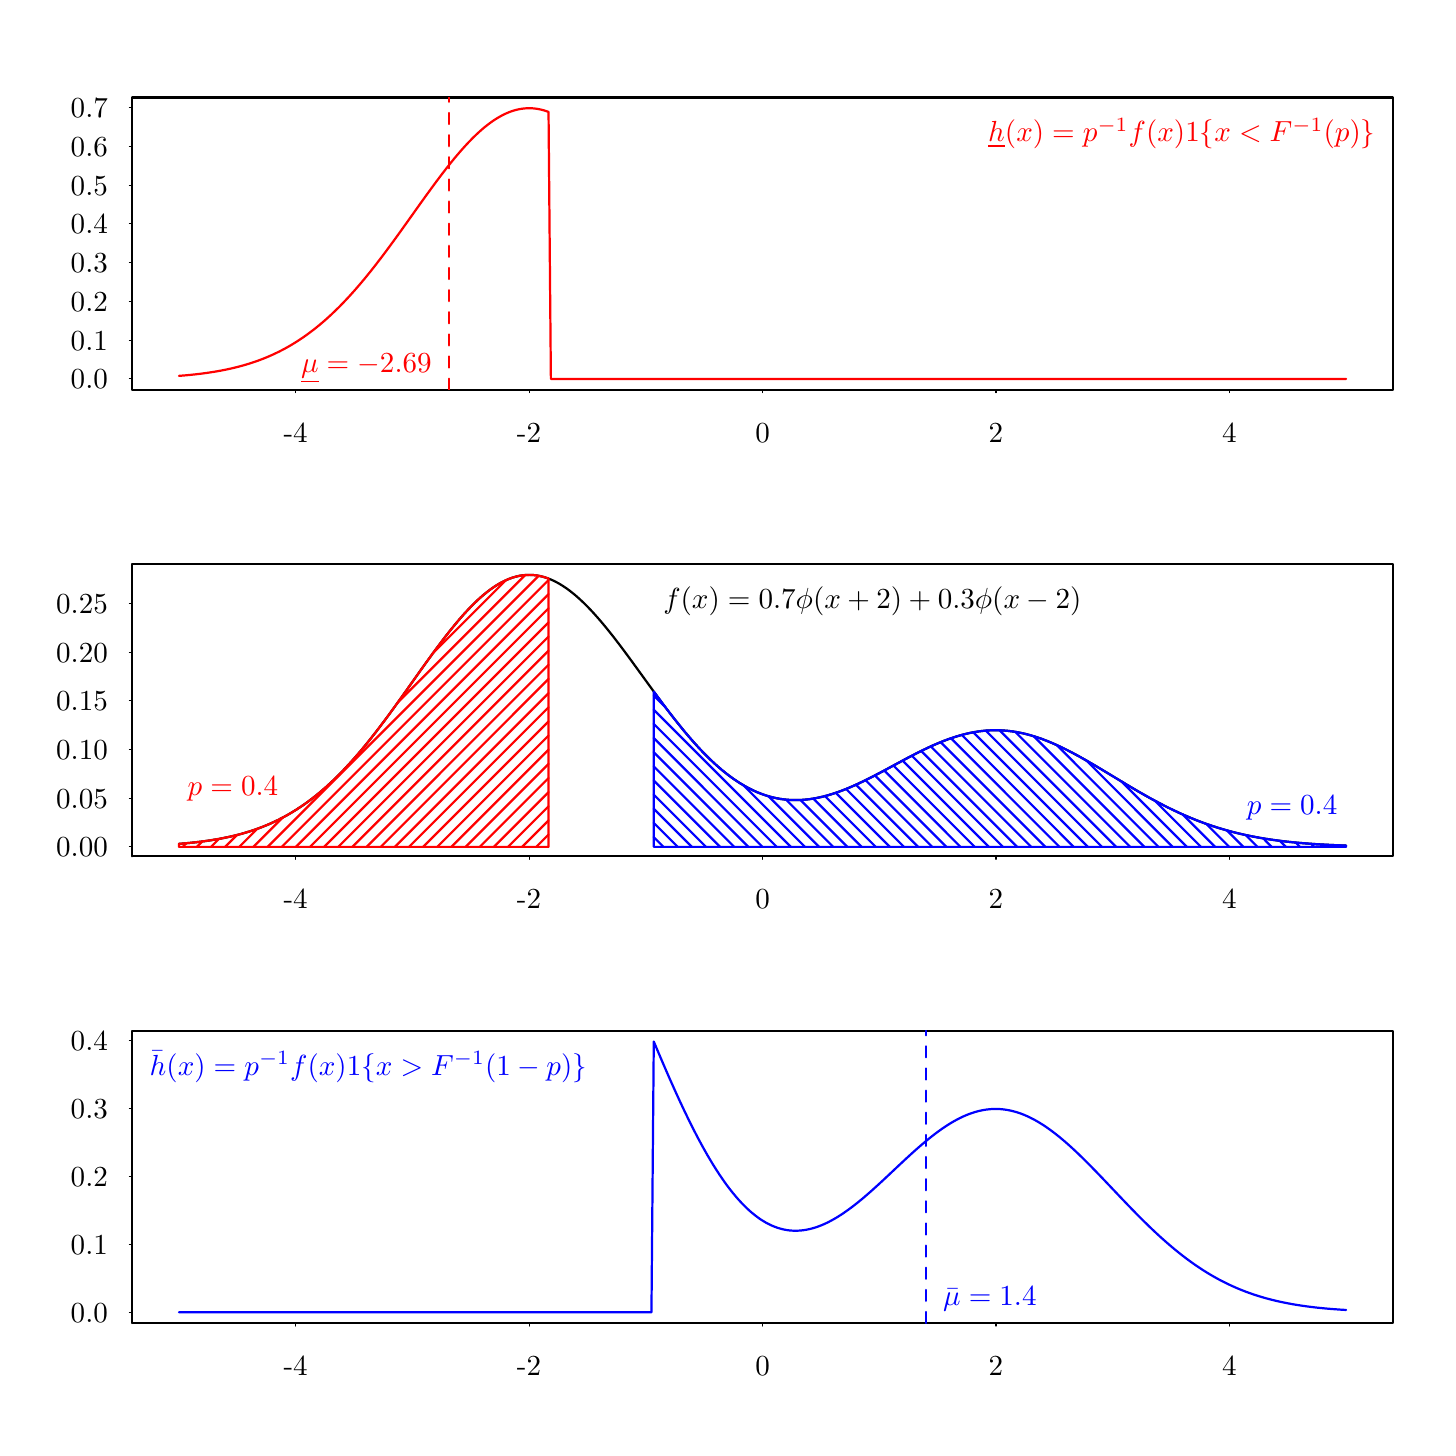
\begin{tikzpicture}[x=1pt,y=1pt]
\definecolor{fillColor}{RGB}{255,255,255}
\path[use as bounding box,fill=fillColor,fill opacity=0.00] (0,0) rectangle (505.89,505.89);
\begin{scope}
\path[clip] ( 37.80,375.06) rectangle (493.29,480.69);
\definecolor{drawColor}{RGB}{255,0,0}

\path[draw=drawColor,line width= 0.8pt,line join=round,line cap=round] ( 54.67,380.06) --
	( 55.52,380.13) --
	( 56.36,380.20) --
	( 57.21,380.27) --
	( 58.05,380.35) --
	( 58.90,380.43) --
	( 59.74,380.52) --
	( 60.59,380.61) --
	( 61.43,380.71) --
	( 62.28,380.81) --
	( 63.12,380.91) --
	( 63.97,381.03) --
	( 64.81,381.14) --
	( 65.66,381.27) --
	( 66.50,381.40) --
	( 67.35,381.53) --
	( 68.19,381.67) --
	( 69.04,381.82) --
	( 69.88,381.98) --
	( 70.73,382.14) --
	( 71.57,382.31) --
	( 72.42,382.49) --
	( 73.26,382.67) --
	( 74.11,382.87) --
	( 74.95,383.07) --
	( 75.80,383.28) --
	( 76.64,383.50) --
	( 77.49,383.73) --
	( 78.34,383.97) --
	( 79.18,384.22) --
	( 80.03,384.48) --
	( 80.87,384.75) --
	( 81.72,385.03) --
	( 82.56,385.32) --
	( 83.41,385.62) --
	( 84.25,385.94) --
	( 85.10,386.27) --
	( 85.94,386.60) --
	( 86.79,386.96) --
	( 87.63,387.32) --
	( 88.48,387.70) --
	( 89.32,388.09) --
	( 90.17,388.50) --
	( 91.01,388.91) --
	( 91.86,389.35) --
	( 92.70,389.79) --
	( 93.55,390.26) --
	( 94.39,390.73) --
	( 95.24,391.23) --
	( 96.08,391.74) --
	( 96.93,392.26) --
	( 97.77,392.80) --
	( 98.62,393.36) --
	( 99.47,393.93) --
	(100.31,394.52) --
	(101.16,395.12) --
	(102.00,395.75) --
	(102.85,396.39) --
	(103.69,397.04) --
	(104.54,397.72) --
	(105.38,398.41) --
	(106.23,399.12) --
	(107.07,399.84) --
	(107.92,400.59) --
	(108.76,401.35) --
	(109.61,402.13) --
	(110.45,402.93) --
	(111.30,403.74) --
	(112.14,404.57) --
	(112.99,405.42) --
	(113.83,406.28) --
	(114.68,407.17) --
	(115.52,408.07) --
	(116.37,408.98) --
	(117.21,409.92) --
	(118.06,410.86) --
	(118.90,411.83) --
	(119.75,412.81) --
	(120.59,413.80) --
	(121.44,414.82) --
	(122.29,415.84) --
	(123.13,416.88) --
	(123.98,417.93) --
	(124.82,419.00) --
	(125.67,420.08) --
	(126.51,421.17) --
	(127.36,422.27) --
	(128.20,423.38) --
	(129.05,424.50) --
	(129.89,425.64) --
	(130.74,426.78) --
	(131.58,427.93) --
	(132.43,429.09) --
	(133.27,430.25) --
	(134.12,431.42) --
	(134.96,432.60) --
	(135.81,433.78) --
	(136.65,434.96) --
	(137.50,436.15) --
	(138.34,437.34) --
	(139.19,438.52) --
	(140.03,439.71) --
	(140.88,440.90) --
	(141.72,442.09) --
	(142.57,443.27) --
	(143.41,444.45) --
	(144.26,445.62) --
	(145.11,446.78) --
	(145.95,447.94) --
	(146.80,449.09) --
	(147.64,450.24) --
	(148.49,451.37) --
	(149.33,452.49) --
	(150.18,453.59) --
	(151.02,454.68) --
	(151.87,455.76) --
	(152.71,456.82) --
	(153.56,457.87) --
	(154.40,458.90) --
	(155.25,459.90) --
	(156.09,460.89) --
	(156.94,461.86) --
	(157.78,462.80) --
	(158.63,463.72) --
	(159.47,464.62) --
	(160.32,465.49) --
	(161.16,466.34) --
	(162.01,467.15) --
	(162.85,467.94) --
	(163.70,468.71) --
	(164.54,469.44) --
	(165.39,470.14) --
	(166.24,470.81) --
	(167.08,471.44) --
	(167.93,472.05) --
	(168.77,472.62) --
	(169.62,473.15) --
	(170.46,473.65) --
	(171.31,474.12) --
	(172.15,474.55) --
	(173.00,474.94) --
	(173.84,475.30) --
	(174.69,475.62) --
	(175.53,475.90) --
	(176.38,476.14) --
	(177.22,476.34) --
	(178.07,476.51) --
	(178.91,476.63) --
	(179.76,476.72) --
	(180.60,476.77) --
	(181.45,476.78) --
	(182.29,476.75) --
	(183.14,476.68) --
	(183.98,476.57) --
	(184.83,476.42) --
	(185.67,476.24) --
	(186.52,476.01) --
	(187.36,475.75) --
	(188.21,475.45) --
	(189.06,378.97) --
	(189.90,378.97) --
	(190.75,378.97) --
	(191.59,378.97) --
	(192.44,378.97) --
	(193.28,378.97) --
	(194.13,378.97) --
	(194.97,378.97) --
	(195.82,378.97) --
	(196.66,378.97) --
	(197.51,378.97) --
	(198.35,378.97) --
	(199.20,378.97) --
	(200.04,378.97) --
	(200.89,378.97) --
	(201.73,378.97) --
	(202.58,378.97) --
	(203.42,378.97) --
	(204.27,378.97) --
	(205.11,378.97) --
	(205.96,378.97) --
	(206.80,378.97) --
	(207.65,378.97) --
	(208.49,378.97) --
	(209.34,378.97) --
	(210.19,378.97) --
	(211.03,378.97) --
	(211.88,378.97) --
	(212.72,378.97) --
	(213.57,378.97) --
	(214.41,378.97) --
	(215.26,378.97) --
	(216.10,378.97) --
	(216.95,378.97) --
	(217.79,378.97) --
	(218.64,378.97) --
	(219.48,378.97) --
	(220.33,378.97) --
	(221.17,378.97) --
	(222.02,378.97) --
	(222.86,378.97) --
	(223.71,378.97) --
	(224.55,378.97) --
	(225.40,378.97) --
	(226.24,378.97) --
	(227.09,378.97) --
	(227.93,378.97) --
	(228.78,378.97) --
	(229.62,378.97) --
	(230.47,378.97) --
	(231.31,378.97) --
	(232.16,378.97) --
	(233.01,378.97) --
	(233.85,378.97) --
	(234.70,378.97) --
	(235.54,378.97) --
	(236.39,378.97) --
	(237.23,378.97) --
	(238.08,378.97) --
	(238.92,378.97) --
	(239.77,378.97) --
	(240.61,378.97) --
	(241.46,378.97) --
	(242.30,378.97) --
	(243.15,378.97) --
	(243.99,378.97) --
	(244.84,378.97) --
	(245.68,378.97) --
	(246.53,378.97) --
	(247.37,378.97) --
	(248.22,378.97) --
	(249.06,378.97) --
	(249.91,378.97) --
	(250.75,378.97) --
	(251.60,378.97) --
	(252.44,378.97) --
	(253.29,378.97) --
	(254.13,378.97) --
	(254.98,378.97) --
	(255.83,378.97) --
	(256.67,378.97) --
	(257.52,378.97) --
	(258.36,378.97) --
	(259.21,378.97) --
	(260.05,378.97) --
	(260.90,378.97) --
	(261.74,378.97) --
	(262.59,378.97) --
	(263.43,378.97) --
	(264.28,378.97) --
	(265.12,378.97) --
	(265.97,378.97) --
	(266.81,378.97) --
	(267.66,378.97) --
	(268.50,378.97) --
	(269.35,378.97) --
	(270.19,378.97) --
	(271.04,378.97) --
	(271.88,378.97) --
	(272.73,378.97) --
	(273.57,378.97) --
	(274.42,378.97) --
	(275.26,378.97) --
	(276.11,378.97) --
	(276.96,378.97) --
	(277.80,378.97) --
	(278.65,378.97) --
	(279.49,378.97) --
	(280.34,378.97) --
	(281.18,378.97) --
	(282.03,378.97) --
	(282.87,378.97) --
	(283.72,378.97) --
	(284.56,378.97) --
	(285.41,378.97) --
	(286.25,378.97) --
	(287.10,378.97) --
	(287.94,378.97) --
	(288.79,378.97) --
	(289.63,378.97) --
	(290.48,378.97) --
	(291.32,378.97) --
	(292.17,378.97) --
	(293.01,378.97) --
	(293.86,378.97) --
	(294.70,378.97) --
	(295.55,378.97) --
	(296.39,378.97) --
	(297.24,378.97) --
	(298.08,378.97) --
	(298.93,378.97) --
	(299.78,378.97) --
	(300.62,378.97) --
	(301.47,378.97) --
	(302.31,378.97) --
	(303.16,378.97) --
	(304.00,378.97) --
	(304.85,378.97) --
	(305.69,378.97) --
	(306.54,378.97) --
	(307.38,378.97) --
	(308.23,378.97) --
	(309.07,378.97) --
	(309.92,378.97) --
	(310.76,378.97) --
	(311.61,378.97) --
	(312.45,378.97) --
	(313.30,378.97) --
	(314.14,378.97) --
	(314.99,378.97) --
	(315.83,378.97) --
	(316.68,378.97) --
	(317.52,378.97) --
	(318.37,378.97) --
	(319.21,378.97) --
	(320.06,378.97) --
	(320.90,378.97) --
	(321.75,378.97) --
	(322.60,378.97) --
	(323.44,378.97) --
	(324.29,378.97) --
	(325.13,378.97) --
	(325.98,378.97) --
	(326.82,378.97) --
	(327.67,378.97) --
	(328.51,378.97) --
	(329.36,378.97) --
	(330.20,378.97) --
	(331.05,378.97) --
	(331.89,378.97) --
	(332.74,378.97) --
	(333.58,378.97) --
	(334.43,378.97) --
	(335.27,378.97) --
	(336.12,378.97) --
	(336.96,378.97) --
	(337.81,378.97) --
	(338.65,378.97) --
	(339.50,378.97) --
	(340.34,378.97) --
	(341.19,378.97) --
	(342.03,378.97) --
	(342.88,378.97) --
	(343.73,378.97) --
	(344.57,378.97) --
	(345.42,378.97) --
	(346.26,378.97) --
	(347.11,378.97) --
	(347.95,378.97) --
	(348.80,378.97) --
	(349.64,378.97) --
	(350.49,378.97) --
	(351.33,378.97) --
	(352.18,378.97) --
	(353.02,378.97) --
	(353.87,378.97) --
	(354.71,378.97) --
	(355.56,378.97) --
	(356.40,378.97) --
	(357.25,378.97) --
	(358.09,378.97) --
	(358.94,378.97) --
	(359.78,378.97) --
	(360.63,378.97) --
	(361.47,378.97) --
	(362.32,378.97) --
	(363.16,378.97) --
	(364.01,378.97) --
	(364.85,378.97) --
	(365.70,378.97) --
	(366.55,378.97) --
	(367.39,378.97) --
	(368.24,378.97) --
	(369.08,378.97) --
	(369.93,378.97) --
	(370.77,378.97) --
	(371.62,378.97) --
	(372.46,378.97) --
	(373.31,378.97) --
	(374.15,378.97) --
	(375.00,378.97) --
	(375.84,378.97) --
	(376.69,378.97) --
	(377.53,378.97) --
	(378.38,378.97) --
	(379.22,378.97) --
	(380.07,378.97) --
	(380.91,378.97) --
	(381.76,378.97) --
	(382.60,378.97) --
	(383.45,378.97) --
	(384.29,378.97) --
	(385.14,378.97) --
	(385.98,378.97) --
	(386.83,378.97) --
	(387.68,378.97) --
	(388.52,378.97) --
	(389.37,378.97) --
	(390.21,378.97) --
	(391.06,378.97) --
	(391.90,378.97) --
	(392.75,378.97) --
	(393.59,378.97) --
	(394.44,378.97) --
	(395.28,378.97) --
	(396.13,378.97) --
	(396.97,378.97) --
	(397.82,378.97) --
	(398.66,378.97) --
	(399.51,378.97) --
	(400.35,378.97) --
	(401.20,378.97) --
	(402.04,378.97) --
	(402.89,378.97) --
	(403.73,378.97) --
	(404.58,378.97) --
	(405.42,378.97) --
	(406.27,378.97) --
	(407.11,378.97) --
	(407.96,378.97) --
	(408.80,378.97) --
	(409.65,378.97) --
	(410.50,378.97) --
	(411.34,378.97) --
	(412.19,378.97) --
	(413.03,378.97) --
	(413.88,378.97) --
	(414.72,378.97) --
	(415.57,378.97) --
	(416.41,378.97) --
	(417.26,378.97) --
	(418.10,378.97) --
	(418.95,378.97) --
	(419.79,378.97) --
	(420.64,378.97) --
	(421.48,378.97) --
	(422.33,378.97) --
	(423.17,378.97) --
	(424.02,378.97) --
	(424.86,378.97) --
	(425.71,378.97) --
	(426.55,378.97) --
	(427.40,378.97) --
	(428.24,378.97) --
	(429.09,378.97) --
	(429.93,378.97) --
	(430.78,378.97) --
	(431.62,378.97) --
	(432.47,378.97) --
	(433.32,378.97) --
	(434.16,378.97) --
	(435.01,378.97) --
	(435.85,378.97) --
	(436.70,378.97) --
	(437.54,378.97) --
	(438.39,378.97) --
	(439.23,378.97) --
	(440.08,378.97) --
	(440.92,378.97) --
	(441.77,378.97) --
	(442.61,378.97) --
	(443.46,378.97) --
	(444.30,378.97) --
	(445.15,378.97) --
	(445.99,378.97) --
	(446.84,378.97) --
	(447.68,378.97) --
	(448.53,378.97) --
	(449.37,378.97) --
	(450.22,378.97) --
	(451.06,378.97) --
	(451.91,378.97) --
	(452.75,378.97) --
	(453.60,378.97) --
	(454.45,378.97) --
	(455.29,378.97) --
	(456.14,378.97) --
	(456.98,378.97) --
	(457.83,378.97) --
	(458.67,378.97) --
	(459.52,378.97) --
	(460.36,378.97) --
	(461.21,378.97) --
	(462.05,378.97) --
	(462.90,378.97) --
	(463.74,378.97) --
	(464.59,378.97) --
	(465.43,378.97) --
	(466.28,378.97) --
	(467.12,378.97) --
	(467.97,378.97) --
	(468.81,378.97) --
	(469.66,378.97) --
	(470.50,378.97) --
	(471.35,378.97) --
	(472.19,378.97) --
	(473.04,378.97) --
	(473.88,378.97) --
	(474.73,378.97) --
	(475.57,378.97) --
	(476.42,378.97);
\end{scope}
\begin{scope}
\path[clip] (  0.00,  0.00) rectangle (505.89,505.89);
\definecolor{drawColor}{RGB}{0,0,0}

\path[draw=drawColor,line width= 0.4pt,line join=round,line cap=round] ( 96.84,375.06) -- (434.25,375.06);

\path[draw=drawColor,line width= 0.4pt,line join=round,line cap=round] ( 96.84,375.06) -- ( 96.84,374.00);

\path[draw=drawColor,line width= 0.4pt,line join=round,line cap=round] (181.19,375.06) -- (181.19,374.00);

\path[draw=drawColor,line width= 0.4pt,line join=round,line cap=round] (265.54,375.06) -- (265.54,374.00);

\path[draw=drawColor,line width= 0.4pt,line join=round,line cap=round] (349.89,375.06) -- (349.89,374.00);

\path[draw=drawColor,line width= 0.4pt,line join=round,line cap=round] (434.25,375.06) -- (434.25,374.00);

\node[text=drawColor,anchor=base,inner sep=0pt, outer sep=0pt, scale=  1.05] at ( 96.84,356.16) {-4};

\node[text=drawColor,anchor=base,inner sep=0pt, outer sep=0pt, scale=  1.05] at (181.19,356.16) {-2};

\node[text=drawColor,anchor=base,inner sep=0pt, outer sep=0pt, scale=  1.05] at (265.54,356.16) {0};

\node[text=drawColor,anchor=base,inner sep=0pt, outer sep=0pt, scale=  1.05] at (349.89,356.16) {2};

\node[text=drawColor,anchor=base,inner sep=0pt, outer sep=0pt, scale=  1.05] at (434.25,356.16) {4};

\path[draw=drawColor,line width= 0.4pt,line join=round,line cap=round] ( 37.80,378.97) -- ( 37.80,477.02);

\path[draw=drawColor,line width= 0.4pt,line join=round,line cap=round] ( 37.80,378.97) -- ( 36.74,378.97);

\path[draw=drawColor,line width= 0.4pt,line join=round,line cap=round] ( 37.80,392.98) -- ( 36.74,392.98);

\path[draw=drawColor,line width= 0.4pt,line join=round,line cap=round] ( 37.80,406.99) -- ( 36.74,406.99);

\path[draw=drawColor,line width= 0.4pt,line join=round,line cap=round] ( 37.80,420.99) -- ( 36.74,420.99);

\path[draw=drawColor,line width= 0.4pt,line join=round,line cap=round] ( 37.80,435.00) -- ( 36.74,435.00);

\path[draw=drawColor,line width= 0.4pt,line join=round,line cap=round] ( 37.80,449.01) -- ( 36.74,449.01);

\path[draw=drawColor,line width= 0.4pt,line join=round,line cap=round] ( 37.80,463.02) -- ( 36.74,463.02);

\path[draw=drawColor,line width= 0.4pt,line join=round,line cap=round] ( 37.80,477.02) -- ( 36.74,477.02);

\node[text=drawColor,anchor=base east,inner sep=0pt, outer sep=0pt, scale=  1.05] at ( 28.98,375.36) {0.0};

\node[text=drawColor,anchor=base east,inner sep=0pt, outer sep=0pt, scale=  1.05] at ( 28.98,389.36) {0.1};

\node[text=drawColor,anchor=base east,inner sep=0pt, outer sep=0pt, scale=  1.05] at ( 28.98,403.37) {0.2};

\node[text=drawColor,anchor=base east,inner sep=0pt, outer sep=0pt, scale=  1.05] at ( 28.98,417.38) {0.3};

\node[text=drawColor,anchor=base east,inner sep=0pt, outer sep=0pt, scale=  1.05] at ( 28.98,431.39) {0.4};

\node[text=drawColor,anchor=base east,inner sep=0pt, outer sep=0pt, scale=  1.05] at ( 28.98,445.39) {0.5};

\node[text=drawColor,anchor=base east,inner sep=0pt, outer sep=0pt, scale=  1.05] at ( 28.98,459.40) {0.6};

\node[text=drawColor,anchor=base east,inner sep=0pt, outer sep=0pt, scale=  1.05] at ( 28.98,473.41) {0.7};

\path[draw=drawColor,line width= 0.8pt,line join=round,line cap=round] ( 37.80,375.06) --
	(493.29,375.06) --
	(493.29,480.69) --
	( 37.80,480.69) --
	( 37.80,375.06);
\end{scope}
\begin{scope}
\path[clip] ( 37.80,375.06) rectangle (493.29,480.69);
\definecolor{drawColor}{RGB}{255,0,0}

\node[text=drawColor,anchor=base east,inner sep=0pt, outer sep=0pt, scale=  1.05] at (486.99,464.59) {$\underline{h}(x) = p^{-1}f(x) 1\{x < F^{-1}(p)\}$};

\path[draw=drawColor,line width= 0.8pt,dash pattern=on 4pt off 4pt ,line join=round,line cap=round] (152.27,375.06) -- (152.27,480.69);

\node[text=drawColor,anchor=base east,inner sep=0pt, outer sep=0pt, scale=  1.05] at (145.97,381.45) {$\underline{\mu} = -2.69$};
\end{scope}
\begin{scope}
\path[clip] ( 37.80,206.43) rectangle (493.29,312.06);
\definecolor{drawColor}{RGB}{0,0,0}

\path[draw=drawColor,line width= 0.8pt,line join=round,line cap=round] ( 54.67,210.97) --
	( 55.52,211.03) --
	( 56.36,211.10) --
	( 57.21,211.18) --
	( 58.05,211.26) --
	( 58.90,211.34) --
	( 59.74,211.43) --
	( 60.59,211.52) --
	( 61.43,211.62) --
	( 62.28,211.72) --
	( 63.12,211.83) --
	( 63.97,211.94) --
	( 64.81,212.06) --
	( 65.66,212.18) --
	( 66.50,212.31) --
	( 67.35,212.45) --
	( 68.19,212.59) --
	( 69.04,212.74) --
	( 69.88,212.89) --
	( 70.73,213.06) --
	( 71.57,213.23) --
	( 72.42,213.41) --
	( 73.26,213.59) --
	( 74.11,213.79) --
	( 74.95,213.99) --
	( 75.80,214.20) --
	( 76.64,214.42) --
	( 77.49,214.65) --
	( 78.34,214.90) --
	( 79.18,215.15) --
	( 80.03,215.41) --
	( 80.87,215.68) --
	( 81.72,215.96) --
	( 82.56,216.25) --
	( 83.41,216.56) --
	( 84.25,216.87) --
	( 85.10,217.20) --
	( 85.94,217.54) --
	( 86.79,217.90) --
	( 87.63,218.26) --
	( 88.48,218.64) --
	( 89.32,219.04) --
	( 90.17,219.44) --
	( 91.01,219.86) --
	( 91.86,220.30) --
	( 92.70,220.75) --
	( 93.55,221.21) --
	( 94.39,221.69) --
	( 95.24,222.19) --
	( 96.08,222.70) --
	( 96.93,223.23) --
	( 97.77,223.77) --
	( 98.62,224.33) --
	( 99.47,224.90) --
	(100.31,225.49) --
	(101.16,226.10) --
	(102.00,226.73) --
	(102.85,227.37) --
	(103.69,228.03) --
	(104.54,228.71) --
	(105.38,229.40) --
	(106.23,230.12) --
	(107.07,230.85) --
	(107.92,231.59) --
	(108.76,232.36) --
	(109.61,233.14) --
	(110.45,233.94) --
	(111.30,234.76) --
	(112.14,235.59) --
	(112.99,236.45) --
	(113.83,237.32) --
	(114.68,238.20) --
	(115.52,239.11) --
	(116.37,240.03) --
	(117.21,240.97) --
	(118.06,241.92) --
	(118.90,242.89) --
	(119.75,243.87) --
	(120.59,244.87) --
	(121.44,245.89) --
	(122.29,246.92) --
	(123.13,247.96) --
	(123.98,249.02) --
	(124.82,250.09) --
	(125.67,251.17) --
	(126.51,252.27) --
	(127.36,253.38) --
	(128.20,254.50) --
	(129.05,255.62) --
	(129.89,256.76) --
	(130.74,257.91) --
	(131.58,259.07) --
	(132.43,260.23) --
	(133.27,261.40) --
	(134.12,262.58) --
	(134.96,263.76) --
	(135.81,264.94) --
	(136.65,266.13) --
	(137.50,267.32) --
	(138.34,268.52) --
	(139.19,269.71) --
	(140.03,270.91) --
	(140.88,272.10) --
	(141.72,273.29) --
	(142.57,274.48) --
	(143.41,275.66) --
	(144.26,276.84) --
	(145.11,278.01) --
	(145.95,279.18) --
	(146.80,280.33) --
	(147.64,281.48) --
	(148.49,282.61) --
	(149.33,283.74) --
	(150.18,284.85) --
	(151.02,285.95) --
	(151.87,287.03) --
	(152.71,288.10) --
	(153.56,289.15) --
	(154.40,290.18) --
	(155.25,291.19) --
	(156.09,292.19) --
	(156.94,293.16) --
	(157.78,294.11) --
	(158.63,295.03) --
	(159.47,295.93) --
	(160.32,296.81) --
	(161.16,297.66) --
	(162.01,298.48) --
	(162.85,299.27) --
	(163.70,300.04) --
	(164.54,300.77) --
	(165.39,301.47) --
	(166.24,302.15) --
	(167.08,302.79) --
	(167.93,303.39) --
	(168.77,303.97) --
	(169.62,304.51) --
	(170.46,305.01) --
	(171.31,305.48) --
	(172.15,305.91) --
	(173.00,306.30) --
	(173.84,306.66) --
	(174.69,306.98) --
	(175.53,307.26) --
	(176.38,307.50) --
	(177.22,307.71) --
	(178.07,307.88) --
	(178.91,308.00) --
	(179.76,308.09) --
	(180.60,308.14) --
	(181.45,308.15) --
	(182.29,308.12) --
	(183.14,308.05) --
	(183.98,307.94) --
	(184.83,307.79) --
	(185.67,307.60) --
	(186.52,307.38) --
	(187.36,307.11) --
	(188.21,306.81) --
	(189.06,306.47) --
	(189.90,306.10) --
	(190.75,305.68) --
	(191.59,305.23) --
	(192.44,304.75) --
	(193.28,304.22) --
	(194.13,303.67) --
	(194.97,303.08) --
	(195.82,302.46) --
	(196.66,301.80) --
	(197.51,301.12) --
	(198.35,300.40) --
	(199.20,299.65) --
	(200.04,298.87) --
	(200.89,298.07) --
	(201.73,297.24) --
	(202.58,296.38) --
	(203.42,295.49) --
	(204.27,294.59) --
	(205.11,293.65) --
	(205.96,292.70) --
	(206.80,291.73) --
	(207.65,290.73) --
	(208.49,289.72) --
	(209.34,288.68) --
	(210.19,287.63) --
	(211.03,286.57) --
	(211.88,285.49) --
	(212.72,284.40) --
	(213.57,283.29) --
	(214.41,282.18) --
	(215.26,281.05) --
	(216.10,279.91) --
	(216.95,278.77) --
	(217.79,277.62) --
	(218.64,276.46) --
	(219.48,275.30) --
	(220.33,274.14) --
	(221.17,272.97) --
	(222.02,271.81) --
	(222.86,270.64) --
	(223.71,269.47) --
	(224.55,268.31) --
	(225.40,267.15) --
	(226.24,265.99) --
	(227.09,264.84) --
	(227.93,263.69) --
	(228.78,262.55) --
	(229.62,261.42) --
	(230.47,260.29) --
	(231.31,259.18) --
	(232.16,258.08) --
	(233.01,256.98) --
	(233.85,255.90) --
	(234.70,254.83) --
	(235.54,253.78) --
	(236.39,252.74) --
	(237.23,251.71) --
	(238.08,250.70) --
	(238.92,249.71) --
	(239.77,248.73) --
	(240.61,247.77) --
	(241.46,246.82) --
	(242.30,245.90) --
	(243.15,244.99) --
	(243.99,244.10) --
	(244.84,243.24) --
	(245.68,242.39) --
	(246.53,241.56) --
	(247.37,240.76) --
	(248.22,239.97) --
	(249.06,239.21) --
	(249.91,238.47) --
	(250.75,237.75) --
	(251.60,237.05) --
	(252.44,236.38) --
	(253.29,235.73) --
	(254.13,235.10) --
	(254.98,234.49) --
	(255.83,233.91) --
	(256.67,233.35) --
	(257.52,232.81) --
	(258.36,232.30) --
	(259.21,231.81) --
	(260.05,231.34) --
	(260.90,230.90) --
	(261.74,230.48) --
	(262.59,230.08) --
	(263.43,229.70) --
	(264.28,229.35) --
	(265.12,229.03) --
	(265.97,228.72) --
	(266.81,228.44) --
	(267.66,228.18) --
	(268.50,227.94) --
	(269.35,227.73) --
	(270.19,227.54) --
	(271.04,227.37) --
	(271.88,227.22) --
	(272.73,227.09) --
	(273.57,226.99) --
	(274.42,226.90) --
	(275.26,226.84) --
	(276.11,226.80) --
	(276.96,226.78) --
	(277.80,226.77) --
	(278.65,226.79) --
	(279.49,226.83) --
	(280.34,226.88) --
	(281.18,226.96) --
	(282.03,227.05) --
	(282.87,227.16) --
	(283.72,227.29) --
	(284.56,227.44) --
	(285.41,227.60) --
	(286.25,227.78) --
	(287.10,227.97) --
	(287.94,228.18) --
	(288.79,228.41) --
	(289.63,228.65) --
	(290.48,228.91) --
	(291.32,229.18) --
	(292.17,229.46) --
	(293.01,229.76) --
	(293.86,230.07) --
	(294.70,230.39) --
	(295.55,230.72) --
	(296.39,231.07) --
	(297.24,231.42) --
	(298.08,231.79) --
	(298.93,232.16) --
	(299.78,232.55) --
	(300.62,232.94) --
	(301.47,233.34) --
	(302.31,233.75) --
	(303.16,234.16) --
	(304.00,234.59) --
	(304.85,235.01) --
	(305.69,235.45) --
	(306.54,235.89) --
	(307.38,236.33) --
	(308.23,236.78) --
	(309.07,237.23) --
	(309.92,237.68) --
	(310.76,238.13) --
	(311.61,238.59) --
	(312.45,239.05) --
	(313.30,239.50) --
	(314.14,239.96) --
	(314.99,240.41) --
	(315.83,240.87) --
	(316.68,241.32) --
	(317.52,241.77) --
	(318.37,242.22) --
	(319.21,242.66) --
	(320.06,243.10) --
	(320.90,243.53) --
	(321.75,243.96) --
	(322.60,244.38) --
	(323.44,244.80) --
	(324.29,245.21) --
	(325.13,245.61) --
	(325.98,246.00) --
	(326.82,246.39) --
	(327.67,246.76) --
	(328.51,247.13) --
	(329.36,247.48) --
	(330.20,247.83) --
	(331.05,248.16) --
	(331.89,248.49) --
	(332.74,248.80) --
	(333.58,249.09) --
	(334.43,249.38) --
	(335.27,249.65) --
	(336.12,249.91) --
	(336.96,250.16) --
	(337.81,250.39) --
	(338.65,250.61) --
	(339.50,250.81) --
	(340.34,251.00) --
	(341.19,251.17) --
	(342.03,251.33) --
	(342.88,251.47) --
	(343.73,251.60) --
	(344.57,251.71) --
	(345.42,251.80) --
	(346.26,251.88) --
	(347.11,251.94) --
	(347.95,251.98) --
	(348.80,252.01) --
	(349.64,252.02) --
	(350.49,252.01) --
	(351.33,251.99) --
	(352.18,251.95) --
	(353.02,251.89) --
	(353.87,251.82) --
	(354.71,251.73) --
	(355.56,251.63) --
	(356.40,251.51) --
	(357.25,251.37) --
	(358.09,251.21) --
	(358.94,251.04) --
	(359.78,250.86) --
	(360.63,250.66) --
	(361.47,250.44) --
	(362.32,250.21) --
	(363.16,249.96) --
	(364.01,249.70) --
	(364.85,249.43) --
	(365.70,249.14) --
	(366.55,248.84) --
	(367.39,248.52) --
	(368.24,248.19) --
	(369.08,247.85) --
	(369.93,247.50) --
	(370.77,247.13) --
	(371.62,246.76) --
	(372.46,246.37) --
	(373.31,245.98) --
	(374.15,245.57) --
	(375.00,245.15) --
	(375.84,244.73) --
	(376.69,244.29) --
	(377.53,243.85) --
	(378.38,243.40) --
	(379.22,242.94) --
	(380.07,242.48) --
	(380.91,242.01) --
	(381.76,241.53) --
	(382.60,241.05) --
	(383.45,240.56) --
	(384.29,240.07) --
	(385.14,239.58) --
	(385.98,239.08) --
	(386.83,238.57) --
	(387.68,238.07) --
	(388.52,237.56) --
	(389.37,237.05) --
	(390.21,236.54) --
	(391.06,236.03) --
	(391.90,235.52) --
	(392.75,235.01) --
	(393.59,234.50) --
	(394.44,233.98) --
	(395.28,233.48) --
	(396.13,232.97) --
	(396.97,232.46) --
	(397.82,231.96) --
	(398.66,231.46) --
	(399.51,230.96) --
	(400.35,230.46) --
	(401.20,229.97) --
	(402.04,229.48) --
	(402.89,229.00) --
	(403.73,228.52) --
	(404.58,228.04) --
	(405.42,227.57) --
	(406.27,227.11) --
	(407.11,226.65) --
	(407.96,226.20) --
	(408.80,225.75) --
	(409.65,225.31) --
	(410.50,224.87) --
	(411.34,224.45) --
	(412.19,224.02) --
	(413.03,223.61) --
	(413.88,223.20) --
	(414.72,222.80) --
	(415.57,222.40) --
	(416.41,222.02) --
	(417.26,221.64) --
	(418.10,221.26) --
	(418.95,220.90) --
	(419.79,220.54) --
	(420.64,220.19) --
	(421.48,219.85) --
	(422.33,219.51) --
	(423.17,219.18) --
	(424.02,218.86) --
	(424.86,218.55) --
	(425.71,218.24) --
	(426.55,217.95) --
	(427.40,217.66) --
	(428.24,217.37) --
	(429.09,217.10) --
	(429.93,216.83) --
	(430.78,216.57) --
	(431.62,216.32) --
	(432.47,216.07) --
	(433.32,215.83) --
	(434.16,215.60) --
	(435.01,215.37) --
	(435.85,215.15) --
	(436.70,214.94) --
	(437.54,214.73) --
	(438.39,214.53) --
	(439.23,214.34) --
	(440.08,214.16) --
	(440.92,213.98) --
	(441.77,213.80) --
	(442.61,213.63) --
	(443.46,213.47) --
	(444.30,213.31) --
	(445.15,213.16) --
	(445.99,213.02) --
	(446.84,212.87) --
	(447.68,212.74) --
	(448.53,212.61) --
	(449.37,212.48) --
	(450.22,212.36) --
	(451.06,212.25) --
	(451.91,212.13) --
	(452.75,212.03) --
	(453.60,211.92) --
	(454.45,211.82) --
	(455.29,211.73) --
	(456.14,211.64) --
	(456.98,211.55) --
	(457.83,211.47) --
	(458.67,211.39) --
	(459.52,211.31) --
	(460.36,211.24) --
	(461.21,211.17) --
	(462.05,211.10) --
	(462.90,211.04) --
	(463.74,210.98) --
	(464.59,210.92) --
	(465.43,210.86) --
	(466.28,210.81) --
	(467.12,210.76) --
	(467.97,210.71) --
	(468.81,210.67) --
	(469.66,210.62) --
	(470.50,210.58) --
	(471.35,210.54) --
	(472.19,210.50) --
	(473.04,210.47) --
	(473.88,210.43) --
	(474.73,210.40) --
	(475.57,210.37) --
	(476.42,210.34);
\end{scope}
\begin{scope}
\path[clip] (  0.00,  0.00) rectangle (505.89,505.89);
\definecolor{drawColor}{RGB}{0,0,0}

\path[draw=drawColor,line width= 0.4pt,line join=round,line cap=round] ( 96.84,206.43) -- (434.25,206.43);

\path[draw=drawColor,line width= 0.4pt,line join=round,line cap=round] ( 96.84,206.43) -- ( 96.84,205.37);

\path[draw=drawColor,line width= 0.4pt,line join=round,line cap=round] (181.19,206.43) -- (181.19,205.37);

\path[draw=drawColor,line width= 0.4pt,line join=round,line cap=round] (265.54,206.43) -- (265.54,205.37);

\path[draw=drawColor,line width= 0.4pt,line join=round,line cap=round] (349.89,206.43) -- (349.89,205.37);

\path[draw=drawColor,line width= 0.4pt,line join=round,line cap=round] (434.25,206.43) -- (434.25,205.37);

\node[text=drawColor,anchor=base,inner sep=0pt, outer sep=0pt, scale=  1.05] at ( 96.84,187.53) {-4};

\node[text=drawColor,anchor=base,inner sep=0pt, outer sep=0pt, scale=  1.05] at (181.19,187.53) {-2};

\node[text=drawColor,anchor=base,inner sep=0pt, outer sep=0pt, scale=  1.05] at (265.54,187.53) {0};

\node[text=drawColor,anchor=base,inner sep=0pt, outer sep=0pt, scale=  1.05] at (349.89,187.53) {2};

\node[text=drawColor,anchor=base,inner sep=0pt, outer sep=0pt, scale=  1.05] at (434.25,187.53) {4};

\path[draw=drawColor,line width= 0.4pt,line join=round,line cap=round] ( 37.80,209.87) -- ( 37.80,297.84);

\path[draw=drawColor,line width= 0.4pt,line join=round,line cap=round] ( 37.80,209.87) -- ( 36.74,209.87);

\path[draw=drawColor,line width= 0.4pt,line join=round,line cap=round] ( 37.80,227.47) -- ( 36.74,227.47);

\path[draw=drawColor,line width= 0.4pt,line join=round,line cap=round] ( 37.80,245.06) -- ( 36.74,245.06);

\path[draw=drawColor,line width= 0.4pt,line join=round,line cap=round] ( 37.80,262.65) -- ( 36.74,262.65);

\path[draw=drawColor,line width= 0.4pt,line join=round,line cap=round] ( 37.80,280.25) -- ( 36.74,280.25);

\path[draw=drawColor,line width= 0.4pt,line join=round,line cap=round] ( 37.80,297.84) -- ( 36.74,297.84);

\node[text=drawColor,anchor=base east,inner sep=0pt, outer sep=0pt, scale=  1.05] at ( 28.98,206.26) {0.00};

\node[text=drawColor,anchor=base east,inner sep=0pt, outer sep=0pt, scale=  1.05] at ( 28.98,223.85) {0.05};

\node[text=drawColor,anchor=base east,inner sep=0pt, outer sep=0pt, scale=  1.05] at ( 28.98,241.44) {0.10};

\node[text=drawColor,anchor=base east,inner sep=0pt, outer sep=0pt, scale=  1.05] at ( 28.98,259.04) {0.15};

\node[text=drawColor,anchor=base east,inner sep=0pt, outer sep=0pt, scale=  1.05] at ( 28.98,276.63) {0.20};

\node[text=drawColor,anchor=base east,inner sep=0pt, outer sep=0pt, scale=  1.05] at ( 28.98,294.22) {0.25};

\path[draw=drawColor,line width= 0.8pt,line join=round,line cap=round] ( 37.80,206.43) --
	(493.29,206.43) --
	(493.29,312.06) --
	( 37.80,312.06) --
	( 37.80,206.43);
\end{scope}
\begin{scope}
\path[clip] ( 37.80,206.43) rectangle (493.29,312.06);
\definecolor{drawColor}{RGB}{255,0,0}

\path[draw=drawColor,line width= 0.8pt,line join=round,line cap=round] ( 56.02,209.87) -- ( 57.34,211.19);

\path[draw=drawColor,line width= 0.8pt,line join=round,line cap=round] ( 61.13,209.87) -- ( 63.08,211.82);

\path[draw=drawColor,line width= 0.8pt,line join=round,line cap=round] ( 66.24,209.87) -- ( 69.12,212.75);

\path[draw=drawColor,line width= 0.8pt,line join=round,line cap=round] ( 71.36,209.87) -- ( 75.64,214.16);

\path[draw=drawColor,line width= 0.8pt,line join=round,line cap=round] ( 76.47,209.87) -- ( 83.00,216.41);

\path[draw=drawColor,line width= 0.8pt,line join=round,line cap=round] (146.45,279.86) -- (172.80,306.21);

\path[draw=drawColor,line width= 0.8pt,line join=round,line cap=round] ( 81.58,209.87) -- ( 92.16,220.46);

\path[draw=drawColor,line width= 0.8pt,line join=round,line cap=round] (133.71,262.01) -- (179.79,308.09);

\path[draw=drawColor,line width= 0.8pt,line join=round,line cap=round] ( 86.69,209.87) -- (184.64,307.82);

\path[draw=drawColor,line width= 0.8pt,line join=round,line cap=round] ( 91.80,209.87) -- (188.21,306.29);

\path[draw=drawColor,line width= 0.8pt,line join=round,line cap=round] ( 96.91,209.87) -- (188.21,301.18);

\path[draw=drawColor,line width= 0.8pt,line join=round,line cap=round] (102.02,209.87) -- (188.21,296.07);

\path[draw=drawColor,line width= 0.8pt,line join=round,line cap=round] (107.13,209.87) -- (188.21,290.96);

\path[draw=drawColor,line width= 0.8pt,line join=round,line cap=round] (112.24,209.87) -- (188.21,285.85);

\path[draw=drawColor,line width= 0.8pt,line join=round,line cap=round] (117.35,209.87) -- (188.21,280.74);

\path[draw=drawColor,line width= 0.8pt,line join=round,line cap=round] (122.46,209.87) -- (188.21,275.63);

\path[draw=drawColor,line width= 0.8pt,line join=round,line cap=round] (127.57,209.87) -- (188.21,270.52);

\path[draw=drawColor,line width= 0.8pt,line join=round,line cap=round] (132.68,209.87) -- (188.21,265.41);

\path[draw=drawColor,line width= 0.8pt,line join=round,line cap=round] (137.79,209.87) -- (188.21,260.30);

\path[draw=drawColor,line width= 0.8pt,line join=round,line cap=round] (142.90,209.87) -- (188.21,255.19);

\path[draw=drawColor,line width= 0.8pt,line join=round,line cap=round] (148.01,209.87) -- (188.21,250.08);

\path[draw=drawColor,line width= 0.8pt,line join=round,line cap=round] (153.12,209.87) -- (188.21,244.97);

\path[draw=drawColor,line width= 0.8pt,line join=round,line cap=round] (158.23,209.87) -- (188.21,239.85);

\path[draw=drawColor,line width= 0.8pt,line join=round,line cap=round] (163.34,209.87) -- (188.21,234.74);

\path[draw=drawColor,line width= 0.8pt,line join=round,line cap=round] (168.45,209.87) -- (188.21,229.63);

\path[draw=drawColor,line width= 0.8pt,line join=round,line cap=round] (173.56,209.87) -- (188.21,224.52);

\path[draw=drawColor,line width= 0.8pt,line join=round,line cap=round] (178.67,209.87) -- (188.21,219.41);

\path[draw=drawColor,line width= 0.8pt,line join=round,line cap=round] (183.78,209.87) -- (188.21,214.30);

\path[draw=drawColor,line width= 0.8pt,line join=round,line cap=round] ( 54.67,209.87) --
	( 55.52,209.87) --
	( 56.36,209.87) --
	( 57.21,209.87) --
	( 58.05,209.87) --
	( 58.90,209.87) --
	( 59.74,209.87) --
	( 60.59,209.87) --
	( 61.43,209.87) --
	( 62.28,209.87) --
	( 63.12,209.87) --
	( 63.97,209.87) --
	( 64.81,209.87) --
	( 65.66,209.87) --
	( 66.50,209.87) --
	( 67.35,209.87) --
	( 68.19,209.87) --
	( 69.04,209.87) --
	( 69.88,209.87) --
	( 70.73,209.87) --
	( 71.57,209.87) --
	( 72.42,209.87) --
	( 73.26,209.87) --
	( 74.11,209.87) --
	( 74.95,209.87) --
	( 75.80,209.87) --
	( 76.64,209.87) --
	( 77.49,209.87) --
	( 78.34,209.87) --
	( 79.18,209.87) --
	( 80.03,209.87) --
	( 80.87,209.87) --
	( 81.72,209.87) --
	( 82.56,209.87) --
	( 83.41,209.87) --
	( 84.25,209.87) --
	( 85.10,209.87) --
	( 85.94,209.87) --
	( 86.79,209.87) --
	( 87.63,209.87) --
	( 88.48,209.87) --
	( 89.32,209.87) --
	( 90.17,209.87) --
	( 91.01,209.87) --
	( 91.86,209.87) --
	( 92.70,209.87) --
	( 93.55,209.87) --
	( 94.39,209.87) --
	( 95.24,209.87) --
	( 96.08,209.87) --
	( 96.93,209.87) --
	( 97.77,209.87) --
	( 98.62,209.87) --
	( 99.47,209.87) --
	(100.31,209.87) --
	(101.16,209.87) --
	(102.00,209.87) --
	(102.85,209.87) --
	(103.69,209.87) --
	(104.54,209.87) --
	(105.38,209.87) --
	(106.23,209.87) --
	(107.07,209.87) --
	(107.92,209.87) --
	(108.76,209.87) --
	(109.61,209.87) --
	(110.45,209.87) --
	(111.30,209.87) --
	(112.14,209.87) --
	(112.99,209.87) --
	(113.83,209.87) --
	(114.68,209.87) --
	(115.52,209.87) --
	(116.37,209.87) --
	(117.21,209.87) --
	(118.06,209.87) --
	(118.90,209.87) --
	(119.75,209.87) --
	(120.59,209.87) --
	(121.44,209.87) --
	(122.29,209.87) --
	(123.13,209.87) --
	(123.98,209.87) --
	(124.82,209.87) --
	(125.67,209.87) --
	(126.51,209.87) --
	(127.36,209.87) --
	(128.20,209.87) --
	(129.05,209.87) --
	(129.89,209.87) --
	(130.74,209.87) --
	(131.58,209.87) --
	(132.43,209.87) --
	(133.27,209.87) --
	(134.12,209.87) --
	(134.96,209.87) --
	(135.81,209.87) --
	(136.65,209.87) --
	(137.50,209.87) --
	(138.34,209.87) --
	(139.19,209.87) --
	(140.03,209.87) --
	(140.88,209.87) --
	(141.72,209.87) --
	(142.57,209.87) --
	(143.41,209.87) --
	(144.26,209.87) --
	(145.11,209.87) --
	(145.95,209.87) --
	(146.80,209.87) --
	(147.64,209.87) --
	(148.49,209.87) --
	(149.33,209.87) --
	(150.18,209.87) --
	(151.02,209.87) --
	(151.87,209.87) --
	(152.71,209.87) --
	(153.56,209.87) --
	(154.40,209.87) --
	(155.25,209.87) --
	(156.09,209.87) --
	(156.94,209.87) --
	(157.78,209.87) --
	(158.63,209.87) --
	(159.47,209.87) --
	(160.32,209.87) --
	(161.16,209.87) --
	(162.01,209.87) --
	(162.85,209.87) --
	(163.70,209.87) --
	(164.54,209.87) --
	(165.39,209.87) --
	(166.24,209.87) --
	(167.08,209.87) --
	(167.93,209.87) --
	(168.77,209.87) --
	(169.62,209.87) --
	(170.46,209.87) --
	(171.31,209.87) --
	(172.15,209.87) --
	(173.00,209.87) --
	(173.84,209.87) --
	(174.69,209.87) --
	(175.53,209.87) --
	(176.38,209.87) --
	(177.22,209.87) --
	(178.07,209.87) --
	(178.91,209.87) --
	(179.76,209.87) --
	(180.60,209.87) --
	(181.45,209.87) --
	(182.29,209.87) --
	(183.14,209.87) --
	(183.98,209.87) --
	(184.83,209.87) --
	(185.67,209.87) --
	(186.52,209.87) --
	(187.36,209.87) --
	(188.21,209.87) --
	(188.21,306.81) --
	(187.36,307.11) --
	(186.52,307.38) --
	(185.67,307.60) --
	(184.83,307.79) --
	(183.98,307.94) --
	(183.14,308.05) --
	(182.29,308.12) --
	(181.45,308.15) --
	(180.60,308.14) --
	(179.76,308.09) --
	(178.91,308.00) --
	(178.07,307.88) --
	(177.22,307.71) --
	(176.38,307.50) --
	(175.53,307.26) --
	(174.69,306.98) --
	(173.84,306.66) --
	(173.00,306.30) --
	(172.15,305.91) --
	(171.31,305.48) --
	(170.46,305.01) --
	(169.62,304.51) --
	(168.77,303.97) --
	(167.93,303.39) --
	(167.08,302.79) --
	(166.24,302.15) --
	(165.39,301.47) --
	(164.54,300.77) --
	(163.70,300.04) --
	(162.85,299.27) --
	(162.01,298.48) --
	(161.16,297.66) --
	(160.32,296.81) --
	(159.47,295.93) --
	(158.63,295.03) --
	(157.78,294.11) --
	(156.94,293.16) --
	(156.09,292.19) --
	(155.25,291.19) --
	(154.40,290.18) --
	(153.56,289.15) --
	(152.71,288.10) --
	(151.87,287.03) --
	(151.02,285.95) --
	(150.18,284.85) --
	(149.33,283.74) --
	(148.49,282.61) --
	(147.64,281.48) --
	(146.80,280.33) --
	(145.95,279.18) --
	(145.11,278.01) --
	(144.26,276.84) --
	(143.41,275.66) --
	(142.57,274.48) --
	(141.72,273.29) --
	(140.88,272.10) --
	(140.03,270.91) --
	(139.19,269.71) --
	(138.34,268.52) --
	(137.50,267.32) --
	(136.65,266.13) --
	(135.81,264.94) --
	(134.96,263.76) --
	(134.12,262.58) --
	(133.27,261.40) --
	(132.43,260.23) --
	(131.58,259.07) --
	(130.74,257.91) --
	(129.89,256.76) --
	(129.05,255.62) --
	(128.20,254.50) --
	(127.36,253.38) --
	(126.51,252.27) --
	(125.67,251.17) --
	(124.82,250.09) --
	(123.98,249.02) --
	(123.13,247.96) --
	(122.29,246.92) --
	(121.44,245.89) --
	(120.59,244.87) --
	(119.75,243.87) --
	(118.90,242.89) --
	(118.06,241.92) --
	(117.21,240.97) --
	(116.37,240.03) --
	(115.52,239.11) --
	(114.68,238.20) --
	(113.83,237.32) --
	(112.99,236.45) --
	(112.14,235.59) --
	(111.30,234.76) --
	(110.45,233.94) --
	(109.61,233.14) --
	(108.76,232.36) --
	(107.92,231.59) --
	(107.07,230.85) --
	(106.23,230.12) --
	(105.38,229.40) --
	(104.54,228.71) --
	(103.69,228.03) --
	(102.85,227.37) --
	(102.00,226.73) --
	(101.16,226.10) --
	(100.31,225.49) --
	( 99.47,224.90) --
	( 98.62,224.33) --
	( 97.77,223.77) --
	( 96.93,223.23) --
	( 96.08,222.70) --
	( 95.24,222.19) --
	( 94.39,221.69) --
	( 93.55,221.21) --
	( 92.70,220.75) --
	( 91.86,220.30) --
	( 91.01,219.86) --
	( 90.17,219.44) --
	( 89.32,219.04) --
	( 88.48,218.64) --
	( 87.63,218.26) --
	( 86.79,217.90) --
	( 85.94,217.54) --
	( 85.10,217.20) --
	( 84.25,216.87) --
	( 83.41,216.56) --
	( 82.56,216.25) --
	( 81.72,215.96) --
	( 80.87,215.68) --
	( 80.03,215.41) --
	( 79.18,215.15) --
	( 78.34,214.90) --
	( 77.49,214.65) --
	( 76.64,214.42) --
	( 75.80,214.20) --
	( 74.95,213.99) --
	( 74.11,213.79) --
	( 73.26,213.59) --
	( 72.42,213.41) --
	( 71.57,213.23) --
	( 70.73,213.06) --
	( 69.88,212.89) --
	( 69.04,212.74) --
	( 68.19,212.59) --
	( 67.35,212.45) --
	( 66.50,212.31) --
	( 65.66,212.18) --
	( 64.81,212.06) --
	( 63.97,211.94) --
	( 63.12,211.83) --
	( 62.28,211.72) --
	( 61.43,211.62) --
	( 60.59,211.52) --
	( 59.74,211.43) --
	( 58.90,211.34) --
	( 58.05,211.26) --
	( 57.21,211.18) --
	( 56.36,211.10) --
	( 55.52,211.03) --
	( 54.67,210.97) --
	( 54.67,209.87);

\node[text=drawColor,anchor=base east,inner sep=0pt, outer sep=0pt, scale=  1.05] at ( 90.54,228.58) {$p = 0.4$};
\definecolor{drawColor}{RGB}{0,0,255}

\path[draw=drawColor,line width= 0.8pt,line join=round,line cap=round] (229.77,209.87) -- (226.24,213.40);

\path[draw=drawColor,line width= 0.8pt,line join=round,line cap=round] (234.88,209.87) -- (226.24,218.51);

\path[draw=drawColor,line width= 0.8pt,line join=round,line cap=round] (239.99,209.87) -- (226.24,223.62);

\path[draw=drawColor,line width= 0.8pt,line join=round,line cap=round] (245.10,209.87) -- (226.24,228.73);

\path[draw=drawColor,line width= 0.8pt,line join=round,line cap=round] (250.21,209.87) -- (226.24,233.84);

\path[draw=drawColor,line width= 0.8pt,line join=round,line cap=round] (255.32,209.87) -- (226.24,238.96);

\path[draw=drawColor,line width= 0.8pt,line join=round,line cap=round] (260.43,209.87) -- (226.24,244.07);

\path[draw=drawColor,line width= 0.8pt,line join=round,line cap=round] (265.54,209.87) -- (226.24,249.18);

\path[draw=drawColor,line width= 0.8pt,line join=round,line cap=round] (270.66,209.87) -- (226.24,254.29);

\path[draw=drawColor,line width= 0.8pt,line join=round,line cap=round] (275.77,209.87) -- (226.24,259.40);

\path[draw=drawColor,line width= 0.8pt,line join=round,line cap=round] (280.88,209.87) -- (258.58,232.17);

\path[draw=drawColor,line width= 0.8pt,line join=round,line cap=round] (230.51,260.24) -- (226.24,264.51);

\path[draw=drawColor,line width= 0.8pt,line join=round,line cap=round] (285.99,209.87) -- (267.69,228.17);

\path[draw=drawColor,line width= 0.8pt,line join=round,line cap=round] (291.10,209.87) -- (274.03,226.94);

\path[draw=drawColor,line width= 0.8pt,line join=round,line cap=round] (296.21,209.87) -- (279.26,226.82);

\path[draw=drawColor,line width= 0.8pt,line join=round,line cap=round] (301.32,209.87) -- (283.87,227.32);

\path[draw=drawColor,line width= 0.8pt,line join=round,line cap=round] (306.43,209.87) -- (288.08,228.22);

\path[draw=drawColor,line width= 0.8pt,line join=round,line cap=round] (311.54,209.87) -- (292.01,229.41);

\path[draw=drawColor,line width= 0.8pt,line join=round,line cap=round] (316.65,209.87) -- (295.73,230.79);

\path[draw=drawColor,line width= 0.8pt,line join=round,line cap=round] (321.76,209.87) -- (299.30,232.33);

\path[draw=drawColor,line width= 0.8pt,line join=round,line cap=round] (326.87,209.87) -- (302.77,233.97);

\path[draw=drawColor,line width= 0.8pt,line join=round,line cap=round] (331.98,209.87) -- (306.16,235.69);

\path[draw=drawColor,line width= 0.8pt,line join=round,line cap=round] (337.09,209.87) -- (309.51,237.46);

\path[draw=drawColor,line width= 0.8pt,line join=round,line cap=round] (342.20,209.87) -- (312.83,239.25);

\path[draw=drawColor,line width= 0.8pt,line join=round,line cap=round] (347.31,209.87) -- (316.15,241.04);

\path[draw=drawColor,line width= 0.8pt,line join=round,line cap=round] (352.42,209.87) -- (319.49,242.80);

\path[draw=drawColor,line width= 0.8pt,line join=round,line cap=round] (357.53,209.87) -- (322.88,244.52);

\path[draw=drawColor,line width= 0.8pt,line join=round,line cap=round] (362.64,209.87) -- (326.35,246.17);

\path[draw=drawColor,line width= 0.8pt,line join=round,line cap=round] (367.75,209.87) -- (329.91,247.71);

\path[draw=drawColor,line width= 0.8pt,line join=round,line cap=round] (372.86,209.87) -- (333.63,249.11);

\path[draw=drawColor,line width= 0.8pt,line join=round,line cap=round] (377.97,209.87) -- (337.53,250.32);

\path[draw=drawColor,line width= 0.8pt,line join=round,line cap=round] (383.08,209.87) -- (341.69,251.27);

\path[draw=drawColor,line width= 0.8pt,line join=round,line cap=round] (388.19,209.87) -- (346.20,251.87);

\path[draw=drawColor,line width= 0.8pt,line join=round,line cap=round] (393.30,209.87) -- (351.18,251.99);

\path[draw=drawColor,line width= 0.8pt,line join=round,line cap=round] (398.41,209.87) -- (356.85,251.43);

\path[draw=drawColor,line width= 0.8pt,line join=round,line cap=round] (403.52,209.87) -- (363.56,249.84);

\path[draw=drawColor,line width= 0.8pt,line join=round,line cap=round] (408.63,209.87) -- (371.86,246.65);

\path[draw=drawColor,line width= 0.8pt,line join=round,line cap=round] (413.74,209.87) -- (382.52,241.10);

\path[draw=drawColor,line width= 0.8pt,line join=round,line cap=round] (418.85,209.87) -- (395.21,233.52);

\path[draw=drawColor,line width= 0.8pt,line join=round,line cap=round] (423.96,209.87) -- (407.27,226.57);

\path[draw=drawColor,line width= 0.8pt,line join=round,line cap=round] (429.07,209.87) -- (417.36,221.59);

\path[draw=drawColor,line width= 0.8pt,line join=round,line cap=round] (434.18,209.87) -- (425.87,218.19);

\path[draw=drawColor,line width= 0.8pt,line join=round,line cap=round] (439.29,209.87) -- (433.35,215.82);

\path[draw=drawColor,line width= 0.8pt,line join=round,line cap=round] (444.40,209.87) -- (440.14,214.14);

\path[draw=drawColor,line width= 0.8pt,line join=round,line cap=round] (449.51,209.87) -- (446.45,212.94);

\path[draw=drawColor,line width= 0.8pt,line join=round,line cap=round] (454.62,209.87) -- (452.43,212.07);

\path[draw=drawColor,line width= 0.8pt,line join=round,line cap=round] (459.73,209.87) -- (458.17,211.43);

\path[draw=drawColor,line width= 0.8pt,line join=round,line cap=round] (464.85,209.87) -- (463.74,210.98);

\path[draw=drawColor,line width= 0.8pt,line join=round,line cap=round] (469.96,209.87) -- (469.18,210.65);

\path[draw=drawColor,line width= 0.8pt,line join=round,line cap=round] (475.07,209.87) -- (474.53,210.41);

\path[draw=drawColor,line width= 0.8pt,line join=round,line cap=round] (226.24,209.87) --
	(227.09,209.87) --
	(227.93,209.87) --
	(228.78,209.87) --
	(229.62,209.87) --
	(230.47,209.87) --
	(231.31,209.87) --
	(232.16,209.87) --
	(233.01,209.87) --
	(233.85,209.87) --
	(234.70,209.87) --
	(235.54,209.87) --
	(236.39,209.87) --
	(237.23,209.87) --
	(238.08,209.87) --
	(238.92,209.87) --
	(239.77,209.87) --
	(240.61,209.87) --
	(241.46,209.87) --
	(242.30,209.87) --
	(243.15,209.87) --
	(243.99,209.87) --
	(244.84,209.87) --
	(245.68,209.87) --
	(246.53,209.87) --
	(247.37,209.87) --
	(248.22,209.87) --
	(249.06,209.87) --
	(249.91,209.87) --
	(250.75,209.87) --
	(251.60,209.87) --
	(252.44,209.87) --
	(253.29,209.87) --
	(254.13,209.87) --
	(254.98,209.87) --
	(255.83,209.87) --
	(256.67,209.87) --
	(257.52,209.87) --
	(258.36,209.87) --
	(259.21,209.87) --
	(260.05,209.87) --
	(260.90,209.87) --
	(261.74,209.87) --
	(262.59,209.87) --
	(263.43,209.87) --
	(264.28,209.87) --
	(265.12,209.87) --
	(265.97,209.87) --
	(266.81,209.87) --
	(267.66,209.87) --
	(268.50,209.87) --
	(269.35,209.87) --
	(270.19,209.87) --
	(271.04,209.87) --
	(271.88,209.87) --
	(272.73,209.87) --
	(273.57,209.87) --
	(274.42,209.87) --
	(275.26,209.87) --
	(276.11,209.87) --
	(276.96,209.87) --
	(277.80,209.87) --
	(278.65,209.87) --
	(279.49,209.87) --
	(280.34,209.87) --
	(281.18,209.87) --
	(282.03,209.87) --
	(282.87,209.87) --
	(283.72,209.87) --
	(284.56,209.87) --
	(285.41,209.87) --
	(286.25,209.87) --
	(287.10,209.87) --
	(287.94,209.87) --
	(288.79,209.87) --
	(289.63,209.87) --
	(290.48,209.87) --
	(291.32,209.87) --
	(292.17,209.87) --
	(293.01,209.87) --
	(293.86,209.87) --
	(294.70,209.87) --
	(295.55,209.87) --
	(296.39,209.87) --
	(297.24,209.87) --
	(298.08,209.87) --
	(298.93,209.87) --
	(299.78,209.87) --
	(300.62,209.87) --
	(301.47,209.87) --
	(302.31,209.87) --
	(303.16,209.87) --
	(304.00,209.87) --
	(304.85,209.87) --
	(305.69,209.87) --
	(306.54,209.87) --
	(307.38,209.87) --
	(308.23,209.87) --
	(309.07,209.87) --
	(309.92,209.87) --
	(310.76,209.87) --
	(311.61,209.87) --
	(312.45,209.87) --
	(313.30,209.87) --
	(314.14,209.87) --
	(314.99,209.87) --
	(315.83,209.87) --
	(316.68,209.87) --
	(317.52,209.87) --
	(318.37,209.87) --
	(319.21,209.87) --
	(320.06,209.87) --
	(320.90,209.87) --
	(321.75,209.87) --
	(322.60,209.87) --
	(323.44,209.87) --
	(324.29,209.87) --
	(325.13,209.87) --
	(325.98,209.87) --
	(326.82,209.87) --
	(327.67,209.87) --
	(328.51,209.87) --
	(329.36,209.87) --
	(330.20,209.87) --
	(331.05,209.87) --
	(331.89,209.87) --
	(332.74,209.87) --
	(333.58,209.87) --
	(334.43,209.87) --
	(335.27,209.87) --
	(336.12,209.87) --
	(336.96,209.87) --
	(337.81,209.87) --
	(338.65,209.87) --
	(339.50,209.87) --
	(340.34,209.87) --
	(341.19,209.87) --
	(342.03,209.87) --
	(342.88,209.87) --
	(343.73,209.87) --
	(344.57,209.87) --
	(345.42,209.87) --
	(346.26,209.87) --
	(347.11,209.87) --
	(347.95,209.87) --
	(348.80,209.87) --
	(349.64,209.87) --
	(350.49,209.87) --
	(351.33,209.87) --
	(352.18,209.87) --
	(353.02,209.87) --
	(353.87,209.87) --
	(354.71,209.87) --
	(355.56,209.87) --
	(356.40,209.87) --
	(357.25,209.87) --
	(358.09,209.87) --
	(358.94,209.87) --
	(359.78,209.87) --
	(360.63,209.87) --
	(361.47,209.87) --
	(362.32,209.87) --
	(363.16,209.87) --
	(364.01,209.87) --
	(364.85,209.87) --
	(365.70,209.87) --
	(366.55,209.87) --
	(367.39,209.87) --
	(368.24,209.87) --
	(369.08,209.87) --
	(369.93,209.87) --
	(370.77,209.87) --
	(371.62,209.87) --
	(372.46,209.87) --
	(373.31,209.87) --
	(374.15,209.87) --
	(375.00,209.87) --
	(375.84,209.87) --
	(376.69,209.87) --
	(377.53,209.87) --
	(378.38,209.87) --
	(379.22,209.87) --
	(380.07,209.87) --
	(380.91,209.87) --
	(381.76,209.87) --
	(382.60,209.87) --
	(383.45,209.87) --
	(384.29,209.87) --
	(385.14,209.87) --
	(385.98,209.87) --
	(386.83,209.87) --
	(387.68,209.87) --
	(388.52,209.87) --
	(389.37,209.87) --
	(390.21,209.87) --
	(391.06,209.87) --
	(391.90,209.87) --
	(392.75,209.87) --
	(393.59,209.87) --
	(394.44,209.87) --
	(395.28,209.87) --
	(396.13,209.87) --
	(396.97,209.87) --
	(397.82,209.87) --
	(398.66,209.87) --
	(399.51,209.87) --
	(400.35,209.87) --
	(401.20,209.87) --
	(402.04,209.87) --
	(402.89,209.87) --
	(403.73,209.87) --
	(404.58,209.87) --
	(405.42,209.87) --
	(406.27,209.87) --
	(407.11,209.87) --
	(407.96,209.87) --
	(408.80,209.87) --
	(409.65,209.87) --
	(410.50,209.87) --
	(411.34,209.87) --
	(412.19,209.87) --
	(413.03,209.87) --
	(413.88,209.87) --
	(414.72,209.87) --
	(415.57,209.87) --
	(416.41,209.87) --
	(417.26,209.87) --
	(418.10,209.87) --
	(418.95,209.87) --
	(419.79,209.87) --
	(420.64,209.87) --
	(421.48,209.87) --
	(422.33,209.87) --
	(423.17,209.87) --
	(424.02,209.87) --
	(424.86,209.87) --
	(425.71,209.87) --
	(426.55,209.87) --
	(427.40,209.87) --
	(428.24,209.87) --
	(429.09,209.87) --
	(429.93,209.87) --
	(430.78,209.87) --
	(431.62,209.87) --
	(432.47,209.87) --
	(433.32,209.87) --
	(434.16,209.87) --
	(435.01,209.87) --
	(435.85,209.87) --
	(436.70,209.87) --
	(437.54,209.87) --
	(438.39,209.87) --
	(439.23,209.87) --
	(440.08,209.87) --
	(440.92,209.87) --
	(441.77,209.87) --
	(442.61,209.87) --
	(443.46,209.87) --
	(444.30,209.87) --
	(445.15,209.87) --
	(445.99,209.87) --
	(446.84,209.87) --
	(447.68,209.87) --
	(448.53,209.87) --
	(449.37,209.87) --
	(450.22,209.87) --
	(451.06,209.87) --
	(451.91,209.87) --
	(452.75,209.87) --
	(453.60,209.87) --
	(454.45,209.87) --
	(455.29,209.87) --
	(456.14,209.87) --
	(456.98,209.87) --
	(457.83,209.87) --
	(458.67,209.87) --
	(459.52,209.87) --
	(460.36,209.87) --
	(461.21,209.87) --
	(462.05,209.87) --
	(462.90,209.87) --
	(463.74,209.87) --
	(464.59,209.87) --
	(465.43,209.87) --
	(466.28,209.87) --
	(467.12,209.87) --
	(467.97,209.87) --
	(468.81,209.87) --
	(469.66,209.87) --
	(470.50,209.87) --
	(471.35,209.87) --
	(472.19,209.87) --
	(473.04,209.87) --
	(473.88,209.87) --
	(474.73,209.87) --
	(475.57,209.87) --
	(476.42,209.87) --
	(476.42,210.34) --
	(475.57,210.37) --
	(474.73,210.40) --
	(473.88,210.43) --
	(473.04,210.47) --
	(472.19,210.50) --
	(471.35,210.54) --
	(470.50,210.58) --
	(469.66,210.62) --
	(468.81,210.67) --
	(467.97,210.71) --
	(467.12,210.76) --
	(466.28,210.81) --
	(465.43,210.86) --
	(464.59,210.92) --
	(463.74,210.98) --
	(462.90,211.04) --
	(462.05,211.10) --
	(461.21,211.17) --
	(460.36,211.24) --
	(459.52,211.31) --
	(458.67,211.39) --
	(457.83,211.47) --
	(456.98,211.55) --
	(456.14,211.64) --
	(455.29,211.73) --
	(454.45,211.82) --
	(453.60,211.92) --
	(452.75,212.03) --
	(451.91,212.13) --
	(451.06,212.25) --
	(450.22,212.36) --
	(449.37,212.48) --
	(448.53,212.61) --
	(447.68,212.74) --
	(446.84,212.87) --
	(445.99,213.02) --
	(445.15,213.16) --
	(444.30,213.31) --
	(443.46,213.47) --
	(442.61,213.63) --
	(441.77,213.80) --
	(440.92,213.98) --
	(440.08,214.16) --
	(439.23,214.34) --
	(438.39,214.53) --
	(437.54,214.73) --
	(436.70,214.94) --
	(435.85,215.15) --
	(435.01,215.37) --
	(434.16,215.60) --
	(433.32,215.83) --
	(432.47,216.07) --
	(431.62,216.32) --
	(430.78,216.57) --
	(429.93,216.83) --
	(429.09,217.10) --
	(428.24,217.37) --
	(427.40,217.66) --
	(426.55,217.95) --
	(425.71,218.24) --
	(424.86,218.55) --
	(424.02,218.86) --
	(423.17,219.18) --
	(422.33,219.51) --
	(421.48,219.85) --
	(420.64,220.19) --
	(419.79,220.54) --
	(418.95,220.90) --
	(418.10,221.26) --
	(417.26,221.64) --
	(416.41,222.02) --
	(415.57,222.40) --
	(414.72,222.80) --
	(413.88,223.20) --
	(413.03,223.61) --
	(412.19,224.02) --
	(411.34,224.45) --
	(410.50,224.87) --
	(409.65,225.31) --
	(408.80,225.75) --
	(407.96,226.20) --
	(407.11,226.65) --
	(406.27,227.11) --
	(405.42,227.57) --
	(404.58,228.04) --
	(403.73,228.52) --
	(402.89,229.00) --
	(402.04,229.48) --
	(401.20,229.97) --
	(400.35,230.46) --
	(399.51,230.96) --
	(398.66,231.46) --
	(397.82,231.96) --
	(396.97,232.46) --
	(396.13,232.97) --
	(395.28,233.48) --
	(394.44,233.98) --
	(393.59,234.50) --
	(392.75,235.01) --
	(391.90,235.52) --
	(391.06,236.03) --
	(390.21,236.54) --
	(389.37,237.05) --
	(388.52,237.56) --
	(387.68,238.07) --
	(386.83,238.57) --
	(385.98,239.08) --
	(385.14,239.58) --
	(384.29,240.07) --
	(383.45,240.56) --
	(382.60,241.05) --
	(381.76,241.53) --
	(380.91,242.01) --
	(380.07,242.48) --
	(379.22,242.94) --
	(378.38,243.40) --
	(377.53,243.85) --
	(376.69,244.29) --
	(375.84,244.73) --
	(375.00,245.15) --
	(374.15,245.57) --
	(373.31,245.98) --
	(372.46,246.37) --
	(371.62,246.76) --
	(370.77,247.13) --
	(369.93,247.50) --
	(369.08,247.85) --
	(368.24,248.19) --
	(367.39,248.52) --
	(366.55,248.84) --
	(365.70,249.14) --
	(364.85,249.43) --
	(364.01,249.70) --
	(363.16,249.96) --
	(362.32,250.21) --
	(361.47,250.44) --
	(360.63,250.66) --
	(359.78,250.86) --
	(358.94,251.04) --
	(358.09,251.21) --
	(357.25,251.37) --
	(356.40,251.51) --
	(355.56,251.63) --
	(354.71,251.73) --
	(353.87,251.82) --
	(353.02,251.89) --
	(352.18,251.95) --
	(351.33,251.99) --
	(350.49,252.01) --
	(349.64,252.02) --
	(348.80,252.01) --
	(347.95,251.98) --
	(347.11,251.94) --
	(346.26,251.88) --
	(345.42,251.80) --
	(344.57,251.71) --
	(343.73,251.60) --
	(342.88,251.47) --
	(342.03,251.33) --
	(341.19,251.17) --
	(340.34,251.00) --
	(339.50,250.81) --
	(338.65,250.61) --
	(337.81,250.39) --
	(336.96,250.16) --
	(336.12,249.91) --
	(335.27,249.65) --
	(334.43,249.38) --
	(333.58,249.09) --
	(332.74,248.80) --
	(331.89,248.49) --
	(331.05,248.16) --
	(330.20,247.83) --
	(329.36,247.48) --
	(328.51,247.13) --
	(327.67,246.76) --
	(326.82,246.39) --
	(325.98,246.00) --
	(325.13,245.61) --
	(324.29,245.21) --
	(323.44,244.80) --
	(322.60,244.38) --
	(321.75,243.96) --
	(320.90,243.53) --
	(320.06,243.10) --
	(319.21,242.66) --
	(318.37,242.22) --
	(317.52,241.77) --
	(316.68,241.32) --
	(315.83,240.87) --
	(314.99,240.41) --
	(314.14,239.96) --
	(313.30,239.50) --
	(312.45,239.05) --
	(311.61,238.59) --
	(310.76,238.13) --
	(309.92,237.68) --
	(309.07,237.23) --
	(308.23,236.78) --
	(307.38,236.33) --
	(306.54,235.89) --
	(305.69,235.45) --
	(304.85,235.01) --
	(304.00,234.59) --
	(303.16,234.16) --
	(302.31,233.75) --
	(301.47,233.34) --
	(300.62,232.94) --
	(299.78,232.55) --
	(298.93,232.16) --
	(298.08,231.79) --
	(297.24,231.42) --
	(296.39,231.07) --
	(295.55,230.72) --
	(294.70,230.39) --
	(293.86,230.07) --
	(293.01,229.76) --
	(292.17,229.46) --
	(291.32,229.18) --
	(290.48,228.91) --
	(289.63,228.65) --
	(288.79,228.41) --
	(287.94,228.18) --
	(287.10,227.97) --
	(286.25,227.78) --
	(285.41,227.60) --
	(284.56,227.44) --
	(283.72,227.29) --
	(282.87,227.16) --
	(282.03,227.05) --
	(281.18,226.96) --
	(280.34,226.88) --
	(279.49,226.83) --
	(278.65,226.79) --
	(277.80,226.77) --
	(276.96,226.78) --
	(276.11,226.80) --
	(275.26,226.84) --
	(274.42,226.90) --
	(273.57,226.99) --
	(272.73,227.09) --
	(271.88,227.22) --
	(271.04,227.37) --
	(270.19,227.54) --
	(269.35,227.73) --
	(268.50,227.94) --
	(267.66,228.18) --
	(266.81,228.44) --
	(265.97,228.72) --
	(265.12,229.03) --
	(264.28,229.35) --
	(263.43,229.70) --
	(262.59,230.08) --
	(261.74,230.48) --
	(260.90,230.90) --
	(260.05,231.34) --
	(259.21,231.81) --
	(258.36,232.30) --
	(257.52,232.81) --
	(256.67,233.35) --
	(255.83,233.91) --
	(254.98,234.49) --
	(254.13,235.10) --
	(253.29,235.73) --
	(252.44,236.38) --
	(251.60,237.05) --
	(250.75,237.75) --
	(249.91,238.47) --
	(249.06,239.21) --
	(248.22,239.97) --
	(247.37,240.76) --
	(246.53,241.56) --
	(245.68,242.39) --
	(244.84,243.24) --
	(243.99,244.10) --
	(243.15,244.99) --
	(242.30,245.90) --
	(241.46,246.82) --
	(240.61,247.77) --
	(239.77,248.73) --
	(238.92,249.71) --
	(238.08,250.70) --
	(237.23,251.71) --
	(236.39,252.74) --
	(235.54,253.78) --
	(234.70,254.83) --
	(233.85,255.90) --
	(233.01,256.98) --
	(232.16,258.08) --
	(231.31,259.18) --
	(230.47,260.29) --
	(229.62,261.42) --
	(228.78,262.55) --
	(227.93,263.69) --
	(227.09,264.84) --
	(226.24,265.99) --
	(226.24,209.87);

\node[text=drawColor,anchor=base west,inner sep=0pt, outer sep=0pt, scale=  1.05] at (440.55,221.54) {$p = 0.4$};
\definecolor{drawColor}{RGB}{0,0,0}

\node[text=drawColor,anchor=base west,inner sep=0pt, outer sep=0pt, scale=  1.05] at (229.67,295.91) {$f(x) = 0.7 \phi(x + 2)+0.3\phi(x - 2)$};
\end{scope}
\begin{scope}
\path[clip] ( 37.80, 37.80) rectangle (493.29,143.43);
\definecolor{drawColor}{RGB}{0,0,255}

\path[draw=drawColor,line width= 0.8pt,line join=round,line cap=round] ( 54.67, 41.71) --
	( 55.52, 41.71) --
	( 56.36, 41.71) --
	( 57.21, 41.71) --
	( 58.05, 41.71) --
	( 58.90, 41.71) --
	( 59.74, 41.71) --
	( 60.59, 41.71) --
	( 61.43, 41.71) --
	( 62.28, 41.71) --
	( 63.12, 41.71) --
	( 63.97, 41.71) --
	( 64.81, 41.71) --
	( 65.66, 41.71) --
	( 66.50, 41.71) --
	( 67.35, 41.71) --
	( 68.19, 41.71) --
	( 69.04, 41.71) --
	( 69.88, 41.71) --
	( 70.73, 41.71) --
	( 71.57, 41.71) --
	( 72.42, 41.71) --
	( 73.26, 41.71) --
	( 74.11, 41.71) --
	( 74.95, 41.71) --
	( 75.80, 41.71) --
	( 76.64, 41.71) --
	( 77.49, 41.71) --
	( 78.34, 41.71) --
	( 79.18, 41.71) --
	( 80.03, 41.71) --
	( 80.87, 41.71) --
	( 81.72, 41.71) --
	( 82.56, 41.71) --
	( 83.41, 41.71) --
	( 84.25, 41.71) --
	( 85.10, 41.71) --
	( 85.94, 41.71) --
	( 86.79, 41.71) --
	( 87.63, 41.71) --
	( 88.48, 41.71) --
	( 89.32, 41.71) --
	( 90.17, 41.71) --
	( 91.01, 41.71) --
	( 91.86, 41.71) --
	( 92.70, 41.71) --
	( 93.55, 41.71) --
	( 94.39, 41.71) --
	( 95.24, 41.71) --
	( 96.08, 41.71) --
	( 96.93, 41.71) --
	( 97.77, 41.71) --
	( 98.62, 41.71) --
	( 99.47, 41.71) --
	(100.31, 41.71) --
	(101.16, 41.71) --
	(102.00, 41.71) --
	(102.85, 41.71) --
	(103.69, 41.71) --
	(104.54, 41.71) --
	(105.38, 41.71) --
	(106.23, 41.71) --
	(107.07, 41.71) --
	(107.92, 41.71) --
	(108.76, 41.71) --
	(109.61, 41.71) --
	(110.45, 41.71) --
	(111.30, 41.71) --
	(112.14, 41.71) --
	(112.99, 41.71) --
	(113.83, 41.71) --
	(114.68, 41.71) --
	(115.52, 41.71) --
	(116.37, 41.71) --
	(117.21, 41.71) --
	(118.06, 41.71) --
	(118.90, 41.71) --
	(119.75, 41.71) --
	(120.59, 41.71) --
	(121.44, 41.71) --
	(122.29, 41.71) --
	(123.13, 41.71) --
	(123.98, 41.71) --
	(124.82, 41.71) --
	(125.67, 41.71) --
	(126.51, 41.71) --
	(127.36, 41.71) --
	(128.20, 41.71) --
	(129.05, 41.71) --
	(129.89, 41.71) --
	(130.74, 41.71) --
	(131.58, 41.71) --
	(132.43, 41.71) --
	(133.27, 41.71) --
	(134.12, 41.71) --
	(134.96, 41.71) --
	(135.81, 41.71) --
	(136.65, 41.71) --
	(137.50, 41.71) --
	(138.34, 41.71) --
	(139.19, 41.71) --
	(140.03, 41.71) --
	(140.88, 41.71) --
	(141.72, 41.71) --
	(142.57, 41.71) --
	(143.41, 41.71) --
	(144.26, 41.71) --
	(145.11, 41.71) --
	(145.95, 41.71) --
	(146.80, 41.71) --
	(147.64, 41.71) --
	(148.49, 41.71) --
	(149.33, 41.71) --
	(150.18, 41.71) --
	(151.02, 41.71) --
	(151.87, 41.71) --
	(152.71, 41.71) --
	(153.56, 41.71) --
	(154.40, 41.71) --
	(155.25, 41.71) --
	(156.09, 41.71) --
	(156.94, 41.71) --
	(157.78, 41.71) --
	(158.63, 41.71) --
	(159.47, 41.71) --
	(160.32, 41.71) --
	(161.16, 41.71) --
	(162.01, 41.71) --
	(162.85, 41.71) --
	(163.70, 41.71) --
	(164.54, 41.71) --
	(165.39, 41.71) --
	(166.24, 41.71) --
	(167.08, 41.71) --
	(167.93, 41.71) --
	(168.77, 41.71) --
	(169.62, 41.71) --
	(170.46, 41.71) --
	(171.31, 41.71) --
	(172.15, 41.71) --
	(173.00, 41.71) --
	(173.84, 41.71) --
	(174.69, 41.71) --
	(175.53, 41.71) --
	(176.38, 41.71) --
	(177.22, 41.71) --
	(178.07, 41.71) --
	(178.91, 41.71) --
	(179.76, 41.71) --
	(180.60, 41.71) --
	(181.45, 41.71) --
	(182.29, 41.71) --
	(183.14, 41.71) --
	(183.98, 41.71) --
	(184.83, 41.71) --
	(185.67, 41.71) --
	(186.52, 41.71) --
	(187.36, 41.71) --
	(188.21, 41.71) --
	(189.06, 41.71) --
	(189.90, 41.71) --
	(190.75, 41.71) --
	(191.59, 41.71) --
	(192.44, 41.71) --
	(193.28, 41.71) --
	(194.13, 41.71) --
	(194.97, 41.71) --
	(195.82, 41.71) --
	(196.66, 41.71) --
	(197.51, 41.71) --
	(198.35, 41.71) --
	(199.20, 41.71) --
	(200.04, 41.71) --
	(200.89, 41.71) --
	(201.73, 41.71) --
	(202.58, 41.71) --
	(203.42, 41.71) --
	(204.27, 41.71) --
	(205.11, 41.71) --
	(205.96, 41.71) --
	(206.80, 41.71) --
	(207.65, 41.71) --
	(208.49, 41.71) --
	(209.34, 41.71) --
	(210.19, 41.71) --
	(211.03, 41.71) --
	(211.88, 41.71) --
	(212.72, 41.71) --
	(213.57, 41.71) --
	(214.41, 41.71) --
	(215.26, 41.71) --
	(216.10, 41.71) --
	(216.95, 41.71) --
	(217.79, 41.71) --
	(218.64, 41.71) --
	(219.48, 41.71) --
	(220.33, 41.71) --
	(221.17, 41.71) --
	(222.02, 41.71) --
	(222.86, 41.71) --
	(223.71, 41.71) --
	(224.55, 41.71) --
	(225.40, 41.71) --
	(226.24,139.52) --
	(227.09,137.51) --
	(227.93,135.51) --
	(228.78,133.52) --
	(229.62,131.55) --
	(230.47,129.59) --
	(231.31,127.65) --
	(232.16,125.72) --
	(233.01,123.82) --
	(233.85,121.93) --
	(234.70,120.07) --
	(235.54,118.23) --
	(236.39,116.42) --
	(237.23,114.63) --
	(238.08,112.87) --
	(238.92,111.13) --
	(239.77,109.43) --
	(240.61,107.75) --
	(241.46,106.11) --
	(242.30,104.50) --
	(243.15,102.92) --
	(243.99,101.37) --
	(244.84, 99.86) --
	(245.68, 98.38) --
	(246.53, 96.94) --
	(247.37, 95.54) --
	(248.22, 94.17) --
	(249.06, 92.84) --
	(249.91, 91.55) --
	(250.75, 90.30) --
	(251.60, 89.08) --
	(252.44, 87.90) --
	(253.29, 86.77) --
	(254.13, 85.67) --
	(254.98, 84.62) --
	(255.83, 83.60) --
	(256.67, 82.62) --
	(257.52, 81.69) --
	(258.36, 80.79) --
	(259.21, 79.94) --
	(260.05, 79.12) --
	(260.90, 78.35) --
	(261.74, 77.62) --
	(262.59, 76.93) --
	(263.43, 76.28) --
	(264.28, 75.66) --
	(265.12, 75.09) --
	(265.97, 74.56) --
	(266.81, 74.07) --
	(267.66, 73.62) --
	(268.50, 73.21) --
	(269.35, 72.83) --
	(270.19, 72.50) --
	(271.04, 72.20) --
	(271.88, 71.95) --
	(272.73, 71.72) --
	(273.57, 71.54) --
	(274.42, 71.39) --
	(275.26, 71.28) --
	(276.11, 71.21) --
	(276.96, 71.17) --
	(277.80, 71.17) --
	(278.65, 71.20) --
	(279.49, 71.26) --
	(280.34, 71.36) --
	(281.18, 71.49) --
	(282.03, 71.65) --
	(282.87, 71.84) --
	(283.72, 72.07) --
	(284.56, 72.32) --
	(285.41, 72.60) --
	(286.25, 72.92) --
	(287.10, 73.26) --
	(287.94, 73.62) --
	(288.79, 74.02) --
	(289.63, 74.44) --
	(290.48, 74.89) --
	(291.32, 75.36) --
	(292.17, 75.85) --
	(293.01, 76.37) --
	(293.86, 76.91) --
	(294.70, 77.47) --
	(295.55, 78.05) --
	(296.39, 78.65) --
	(297.24, 79.27) --
	(298.08, 79.90) --
	(298.93, 80.56) --
	(299.78, 81.23) --
	(300.62, 81.91) --
	(301.47, 82.61) --
	(302.31, 83.32) --
	(303.16, 84.05) --
	(304.00, 84.78) --
	(304.85, 85.53) --
	(305.69, 86.29) --
	(306.54, 87.05) --
	(307.38, 87.82) --
	(308.23, 88.60) --
	(309.07, 89.38) --
	(309.92, 90.17) --
	(310.76, 90.96) --
	(311.61, 91.76) --
	(312.45, 92.55) --
	(313.30, 93.35) --
	(314.14, 94.15) --
	(314.99, 94.94) --
	(315.83, 95.73) --
	(316.68, 96.52) --
	(317.52, 97.31) --
	(318.37, 98.08) --
	(319.21, 98.86) --
	(320.06, 99.62) --
	(320.90,100.38) --
	(321.75,101.12) --
	(322.60,101.86) --
	(323.44,102.58) --
	(324.29,103.29) --
	(325.13,103.99) --
	(325.98,104.68) --
	(326.82,105.35) --
	(327.67,106.00) --
	(328.51,106.64) --
	(329.36,107.26) --
	(330.20,107.86) --
	(331.05,108.44) --
	(331.89,109.01) --
	(332.74,109.55) --
	(333.58,110.07) --
	(334.43,110.57) --
	(335.27,111.04) --
	(336.12,111.50) --
	(336.96,111.93) --
	(337.81,112.33) --
	(338.65,112.71) --
	(339.50,113.06) --
	(340.34,113.39) --
	(341.19,113.69) --
	(342.03,113.96) --
	(342.88,114.21) --
	(343.73,114.43) --
	(344.57,114.62) --
	(345.42,114.78) --
	(346.26,114.92) --
	(347.11,115.02) --
	(347.95,115.10) --
	(348.80,115.15) --
	(349.64,115.17) --
	(350.49,115.16) --
	(351.33,115.12) --
	(352.18,115.05) --
	(353.02,114.95) --
	(353.87,114.82) --
	(354.71,114.67) --
	(355.56,114.48) --
	(356.40,114.27) --
	(357.25,114.03) --
	(358.09,113.76) --
	(358.94,113.47) --
	(359.78,113.14) --
	(360.63,112.79) --
	(361.47,112.41) --
	(362.32,112.01) --
	(363.16,111.58) --
	(364.01,111.13) --
	(364.85,110.65) --
	(365.70,110.14) --
	(366.55,109.62) --
	(367.39,109.07) --
	(368.24,108.50) --
	(369.08,107.90) --
	(369.93,107.29) --
	(370.77,106.65) --
	(371.62,106.00) --
	(372.46,105.33) --
	(373.31,104.63) --
	(374.15,103.93) --
	(375.00,103.20) --
	(375.84,102.46) --
	(376.69,101.70) --
	(377.53,100.93) --
	(378.38,100.15) --
	(379.22, 99.35) --
	(380.07, 98.54) --
	(380.91, 97.72) --
	(381.76, 96.89) --
	(382.60, 96.05) --
	(383.45, 95.20) --
	(384.29, 94.34) --
	(385.14, 93.48) --
	(385.98, 92.61) --
	(386.83, 91.73) --
	(387.68, 90.85) --
	(388.52, 89.97) --
	(389.37, 89.08) --
	(390.21, 88.19) --
	(391.06, 87.30) --
	(391.90, 86.41) --
	(392.75, 85.52) --
	(393.59, 84.63) --
	(394.44, 83.73) --
	(395.28, 82.85) --
	(396.13, 81.96) --
	(396.97, 81.08) --
	(397.82, 80.20) --
	(398.66, 79.33) --
	(399.51, 78.46) --
	(400.35, 77.59) --
	(401.20, 76.74) --
	(402.04, 75.89) --
	(402.89, 75.04) --
	(403.73, 74.21) --
	(404.58, 73.38) --
	(405.42, 72.56) --
	(406.27, 71.75) --
	(407.11, 70.95) --
	(407.96, 70.16) --
	(408.80, 69.38) --
	(409.65, 68.61) --
	(410.50, 67.86) --
	(411.34, 67.11) --
	(412.19, 66.37) --
	(413.03, 65.65) --
	(413.88, 64.94) --
	(414.72, 64.24) --
	(415.57, 63.55) --
	(416.41, 62.87) --
	(417.26, 62.21) --
	(418.10, 61.56) --
	(418.95, 60.92) --
	(419.79, 60.30) --
	(420.64, 59.69) --
	(421.48, 59.09) --
	(422.33, 58.51) --
	(423.17, 57.94) --
	(424.02, 57.38) --
	(424.86, 56.83) --
	(425.71, 56.30) --
	(426.55, 55.78) --
	(427.40, 55.28) --
	(428.24, 54.78) --
	(429.09, 54.30) --
	(429.93, 53.83) --
	(430.78, 53.38) --
	(431.62, 52.94) --
	(432.47, 52.51) --
	(433.32, 52.09) --
	(434.16, 51.69) --
	(435.01, 51.29) --
	(435.85, 50.91) --
	(436.70, 50.54) --
	(437.54, 50.18) --
	(438.39, 49.83) --
	(439.23, 49.50) --
	(440.08, 49.17) --
	(440.92, 48.86) --
	(441.77, 48.56) --
	(442.61, 48.26) --
	(443.46, 47.98) --
	(444.30, 47.70) --
	(445.15, 47.44) --
	(445.99, 47.19) --
	(446.84, 46.94) --
	(447.68, 46.70) --
	(448.53, 46.48) --
	(449.37, 46.26) --
	(450.22, 46.05) --
	(451.06, 45.84) --
	(451.91, 45.65) --
	(452.75, 45.46) --
	(453.60, 45.28) --
	(454.45, 45.11) --
	(455.29, 44.95) --
	(456.14, 44.79) --
	(456.98, 44.63) --
	(457.83, 44.49) --
	(458.67, 44.35) --
	(459.52, 44.22) --
	(460.36, 44.09) --
	(461.21, 43.97) --
	(462.05, 43.85) --
	(462.90, 43.74) --
	(463.74, 43.63) --
	(464.59, 43.53) --
	(465.43, 43.43) --
	(466.28, 43.34) --
	(467.12, 43.25) --
	(467.97, 43.17) --
	(468.81, 43.09) --
	(469.66, 43.01) --
	(470.50, 42.94) --
	(471.35, 42.87) --
	(472.19, 42.81) --
	(473.04, 42.75) --
	(473.88, 42.69) --
	(474.73, 42.63) --
	(475.57, 42.58) --
	(476.42, 42.53);
\end{scope}
\begin{scope}
\path[clip] (  0.00,  0.00) rectangle (505.89,505.89);
\definecolor{drawColor}{RGB}{0,0,0}

\path[draw=drawColor,line width= 0.4pt,line join=round,line cap=round] ( 96.84, 37.80) -- (434.25, 37.80);

\path[draw=drawColor,line width= 0.4pt,line join=round,line cap=round] ( 96.84, 37.80) -- ( 96.84, 36.74);

\path[draw=drawColor,line width= 0.4pt,line join=round,line cap=round] (181.19, 37.80) -- (181.19, 36.74);

\path[draw=drawColor,line width= 0.4pt,line join=round,line cap=round] (265.54, 37.80) -- (265.54, 36.74);

\path[draw=drawColor,line width= 0.4pt,line join=round,line cap=round] (349.89, 37.80) -- (349.89, 36.74);

\path[draw=drawColor,line width= 0.4pt,line join=round,line cap=round] (434.25, 37.80) -- (434.25, 36.74);

\node[text=drawColor,anchor=base,inner sep=0pt, outer sep=0pt, scale=  1.05] at ( 96.84, 18.90) {-4};

\node[text=drawColor,anchor=base,inner sep=0pt, outer sep=0pt, scale=  1.05] at (181.19, 18.90) {-2};

\node[text=drawColor,anchor=base,inner sep=0pt, outer sep=0pt, scale=  1.05] at (265.54, 18.90) {0};

\node[text=drawColor,anchor=base,inner sep=0pt, outer sep=0pt, scale=  1.05] at (349.89, 18.90) {2};

\node[text=drawColor,anchor=base,inner sep=0pt, outer sep=0pt, scale=  1.05] at (434.25, 18.90) {4};

\path[draw=drawColor,line width= 0.4pt,line join=round,line cap=round] ( 37.80, 41.71) -- ( 37.80,139.83);

\path[draw=drawColor,line width= 0.4pt,line join=round,line cap=round] ( 37.80, 41.71) -- ( 36.74, 41.71);

\path[draw=drawColor,line width= 0.4pt,line join=round,line cap=round] ( 37.80, 66.24) -- ( 36.74, 66.24);

\path[draw=drawColor,line width= 0.4pt,line join=round,line cap=round] ( 37.80, 90.77) -- ( 36.74, 90.77);

\path[draw=drawColor,line width= 0.4pt,line join=round,line cap=round] ( 37.80,115.30) -- ( 36.74,115.30);

\path[draw=drawColor,line width= 0.4pt,line join=round,line cap=round] ( 37.80,139.83) -- ( 36.74,139.83);

\node[text=drawColor,anchor=base east,inner sep=0pt, outer sep=0pt, scale=  1.05] at ( 28.98, 38.10) {0.0};

\node[text=drawColor,anchor=base east,inner sep=0pt, outer sep=0pt, scale=  1.05] at ( 28.98, 62.63) {0.1};

\node[text=drawColor,anchor=base east,inner sep=0pt, outer sep=0pt, scale=  1.05] at ( 28.98, 87.16) {0.2};

\node[text=drawColor,anchor=base east,inner sep=0pt, outer sep=0pt, scale=  1.05] at ( 28.98,111.69) {0.3};

\node[text=drawColor,anchor=base east,inner sep=0pt, outer sep=0pt, scale=  1.05] at ( 28.98,136.22) {0.4};

\path[draw=drawColor,line width= 0.8pt,line join=round,line cap=round] ( 37.80, 37.80) --
	(493.29, 37.80) --
	(493.29,143.43) --
	( 37.80,143.43) --
	( 37.80, 37.80);
\end{scope}
\begin{scope}
\path[clip] ( 37.80, 37.80) rectangle (493.29,143.43);
\definecolor{drawColor}{RGB}{0,0,255}

\node[text=drawColor,anchor=base west,inner sep=0pt, outer sep=0pt, scale=  1.05] at ( 44.10,127.33) {$\bar{h}(x)=p^{-1}f(x)1\{x > F^{-1}(1-p)\}$};

\path[draw=drawColor,line width= 0.8pt,dash pattern=on 4pt off 4pt ,line join=round,line cap=round] (324.52, 37.80) -- (324.52,143.43);

\node[text=drawColor,anchor=base west,inner sep=0pt, outer sep=0pt, scale=  1.05] at (330.82, 44.19) {$\bar{\mu} = 1.4$};
\end{scope}
\end{tikzpicture}

}
\end{figure}

\end{frame}
%%%%%%%%%%%%%%%%%%%%%%%%%%%%%%%%%%%%%%%%%%%%%%%%%%%%%
\begin{frame}[noframenumbering]

\begin{figure}[h]
  \centering
\resizebox{0.85\textwidth}{!}{%
  % Created by tikzDevice version 0.10.1 on 2018-01-15 17:35:20
% !TEX encoding = UTF-8 Unicode
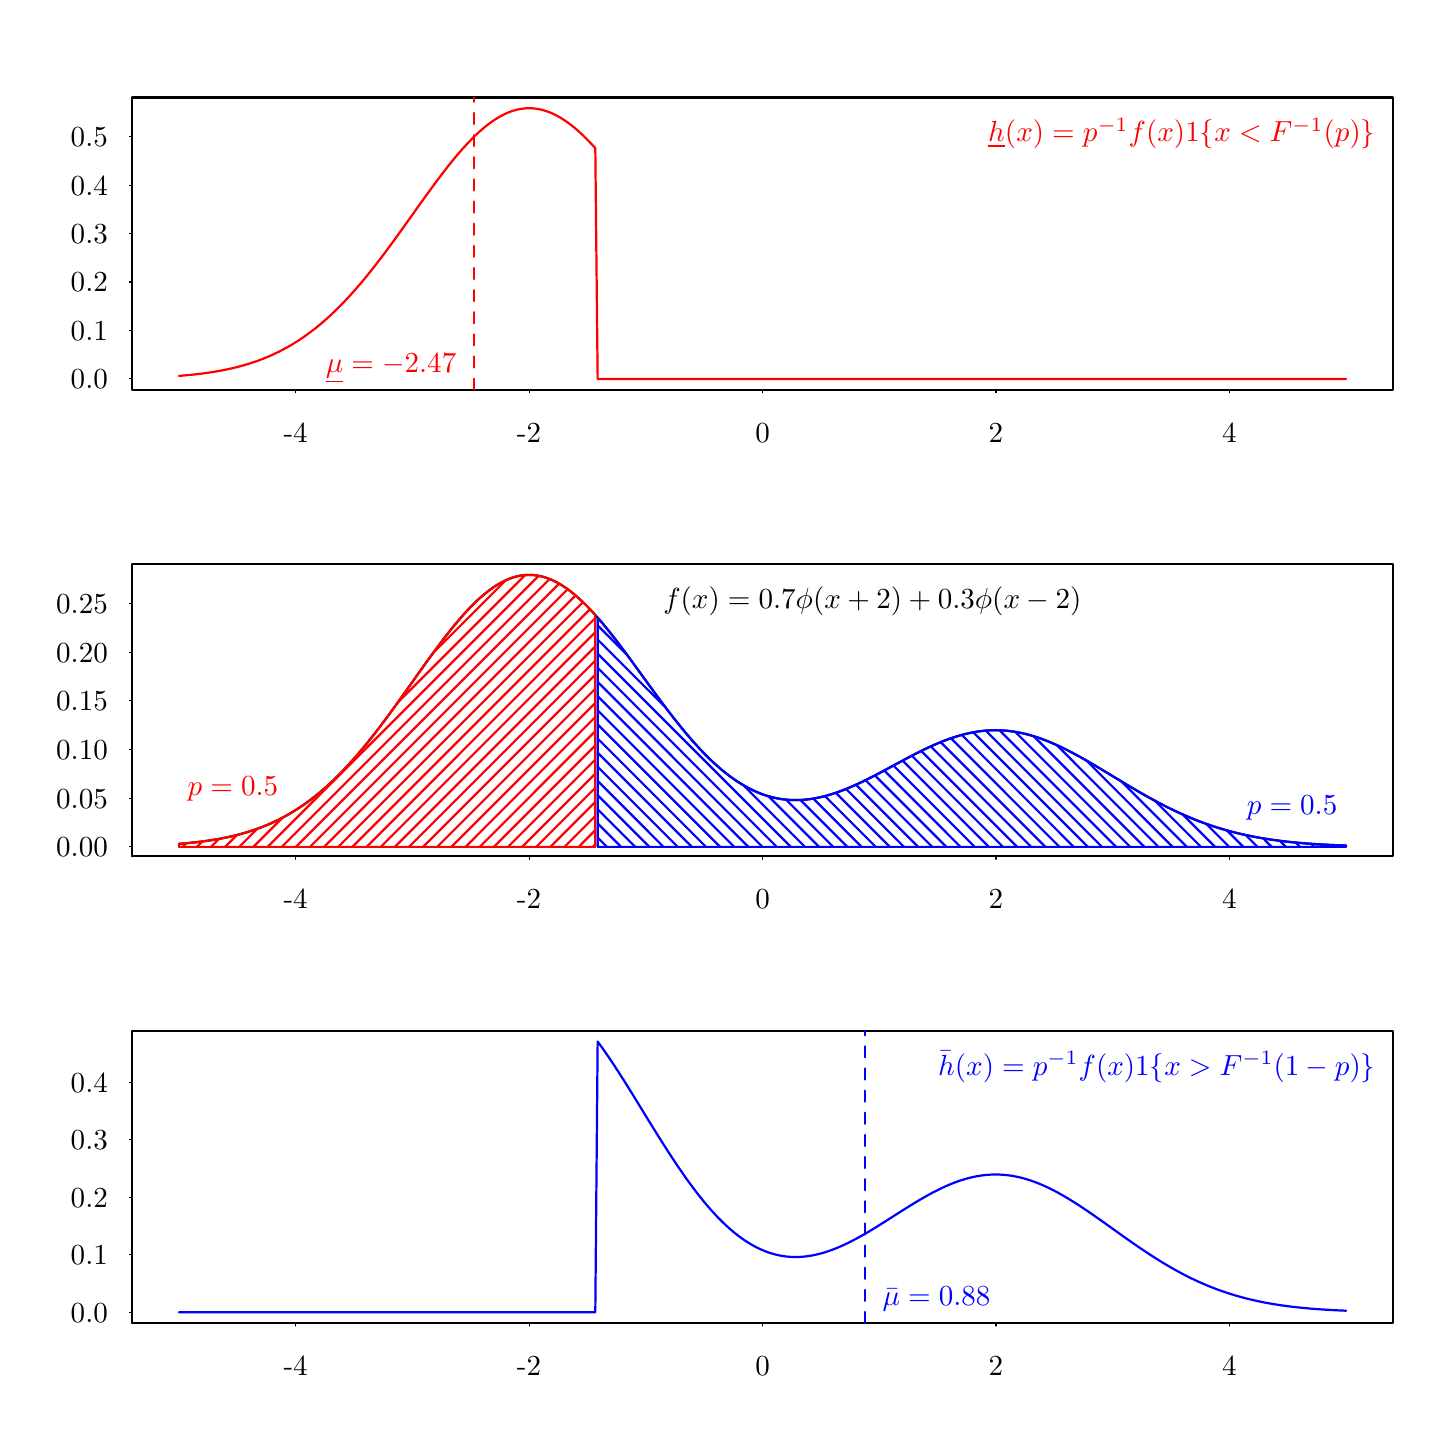
\begin{tikzpicture}[x=1pt,y=1pt]
\definecolor{fillColor}{RGB}{255,255,255}
\path[use as bounding box,fill=fillColor,fill opacity=0.00] (0,0) rectangle (505.89,505.89);
\begin{scope}
\path[clip] ( 37.80,375.06) rectangle (493.29,480.69);
\definecolor{drawColor}{RGB}{255,0,0}

\path[draw=drawColor,line width= 0.8pt,line join=round,line cap=round] ( 54.67,380.06) --
	( 55.52,380.13) --
	( 56.36,380.20) --
	( 57.21,380.27) --
	( 58.05,380.35) --
	( 58.90,380.43) --
	( 59.74,380.52) --
	( 60.59,380.61) --
	( 61.43,380.71) --
	( 62.28,380.81) --
	( 63.12,380.91) --
	( 63.97,381.03) --
	( 64.81,381.14) --
	( 65.66,381.27) --
	( 66.50,381.40) --
	( 67.35,381.53) --
	( 68.19,381.67) --
	( 69.04,381.82) --
	( 69.88,381.98) --
	( 70.73,382.14) --
	( 71.57,382.31) --
	( 72.42,382.49) --
	( 73.26,382.67) --
	( 74.11,382.87) --
	( 74.95,383.07) --
	( 75.80,383.28) --
	( 76.64,383.50) --
	( 77.49,383.73) --
	( 78.34,383.97) --
	( 79.18,384.22) --
	( 80.03,384.48) --
	( 80.87,384.75) --
	( 81.72,385.03) --
	( 82.56,385.32) --
	( 83.41,385.62) --
	( 84.25,385.94) --
	( 85.10,386.27) --
	( 85.94,386.60) --
	( 86.79,386.96) --
	( 87.63,387.32) --
	( 88.48,387.70) --
	( 89.32,388.09) --
	( 90.17,388.50) --
	( 91.01,388.91) --
	( 91.86,389.35) --
	( 92.70,389.79) --
	( 93.55,390.26) --
	( 94.39,390.73) --
	( 95.24,391.23) --
	( 96.08,391.74) --
	( 96.93,392.26) --
	( 97.77,392.80) --
	( 98.62,393.36) --
	( 99.47,393.93) --
	(100.31,394.52) --
	(101.16,395.12) --
	(102.00,395.75) --
	(102.85,396.39) --
	(103.69,397.04) --
	(104.54,397.72) --
	(105.38,398.41) --
	(106.23,399.12) --
	(107.07,399.84) --
	(107.92,400.59) --
	(108.76,401.35) --
	(109.61,402.13) --
	(110.45,402.93) --
	(111.30,403.74) --
	(112.14,404.57) --
	(112.99,405.42) --
	(113.83,406.28) --
	(114.68,407.17) --
	(115.52,408.07) --
	(116.37,408.98) --
	(117.21,409.92) --
	(118.06,410.86) --
	(118.90,411.83) --
	(119.75,412.81) --
	(120.59,413.80) --
	(121.44,414.82) --
	(122.29,415.84) --
	(123.13,416.88) --
	(123.98,417.93) --
	(124.82,419.00) --
	(125.67,420.08) --
	(126.51,421.17) --
	(127.36,422.27) --
	(128.20,423.38) --
	(129.05,424.50) --
	(129.89,425.64) --
	(130.74,426.78) --
	(131.58,427.93) --
	(132.43,429.09) --
	(133.27,430.25) --
	(134.12,431.42) --
	(134.96,432.60) --
	(135.81,433.78) --
	(136.65,434.96) --
	(137.50,436.15) --
	(138.34,437.34) --
	(139.19,438.52) --
	(140.03,439.71) --
	(140.88,440.90) --
	(141.72,442.09) --
	(142.57,443.27) --
	(143.41,444.45) --
	(144.26,445.62) --
	(145.11,446.78) --
	(145.95,447.94) --
	(146.80,449.09) --
	(147.64,450.24) --
	(148.49,451.37) --
	(149.33,452.49) --
	(150.18,453.59) --
	(151.02,454.68) --
	(151.87,455.76) --
	(152.71,456.82) --
	(153.56,457.87) --
	(154.40,458.90) --
	(155.25,459.90) --
	(156.09,460.89) --
	(156.94,461.86) --
	(157.78,462.80) --
	(158.63,463.72) --
	(159.47,464.62) --
	(160.32,465.49) --
	(161.16,466.34) --
	(162.01,467.15) --
	(162.85,467.94) --
	(163.70,468.71) --
	(164.54,469.44) --
	(165.39,470.14) --
	(166.24,470.81) --
	(167.08,471.44) --
	(167.93,472.05) --
	(168.77,472.62) --
	(169.62,473.15) --
	(170.46,473.65) --
	(171.31,474.12) --
	(172.15,474.55) --
	(173.00,474.94) --
	(173.84,475.30) --
	(174.69,475.62) --
	(175.53,475.90) --
	(176.38,476.14) --
	(177.22,476.34) --
	(178.07,476.51) --
	(178.91,476.63) --
	(179.76,476.72) --
	(180.60,476.77) --
	(181.45,476.78) --
	(182.29,476.75) --
	(183.14,476.68) --
	(183.98,476.57) --
	(184.83,476.42) --
	(185.67,476.24) --
	(186.52,476.01) --
	(187.36,475.75) --
	(188.21,475.45) --
	(189.06,475.11) --
	(189.90,474.74) --
	(190.75,474.32) --
	(191.59,473.88) --
	(192.44,473.39) --
	(193.28,472.87) --
	(194.13,472.32) --
	(194.97,471.73) --
	(195.82,471.11) --
	(196.66,470.46) --
	(197.51,469.78) --
	(198.35,469.06) --
	(199.20,468.32) --
	(200.04,467.55) --
	(200.89,466.75) --
	(201.73,465.92) --
	(202.58,465.06) --
	(203.42,464.18) --
	(204.27,463.28) --
	(205.11,462.35) --
	(205.96,378.97) --
	(206.80,378.97) --
	(207.65,378.97) --
	(208.49,378.97) --
	(209.34,378.97) --
	(210.19,378.97) --
	(211.03,378.97) --
	(211.88,378.97) --
	(212.72,378.97) --
	(213.57,378.97) --
	(214.41,378.97) --
	(215.26,378.97) --
	(216.10,378.97) --
	(216.95,378.97) --
	(217.79,378.97) --
	(218.64,378.97) --
	(219.48,378.97) --
	(220.33,378.97) --
	(221.17,378.97) --
	(222.02,378.97) --
	(222.86,378.97) --
	(223.71,378.97) --
	(224.55,378.97) --
	(225.40,378.97) --
	(226.24,378.97) --
	(227.09,378.97) --
	(227.93,378.97) --
	(228.78,378.97) --
	(229.62,378.97) --
	(230.47,378.97) --
	(231.31,378.97) --
	(232.16,378.97) --
	(233.01,378.97) --
	(233.85,378.97) --
	(234.70,378.97) --
	(235.54,378.97) --
	(236.39,378.97) --
	(237.23,378.97) --
	(238.08,378.97) --
	(238.92,378.97) --
	(239.77,378.97) --
	(240.61,378.97) --
	(241.46,378.97) --
	(242.30,378.97) --
	(243.15,378.97) --
	(243.99,378.97) --
	(244.84,378.97) --
	(245.68,378.97) --
	(246.53,378.97) --
	(247.37,378.97) --
	(248.22,378.97) --
	(249.06,378.97) --
	(249.91,378.97) --
	(250.75,378.97) --
	(251.60,378.97) --
	(252.44,378.97) --
	(253.29,378.97) --
	(254.13,378.97) --
	(254.98,378.97) --
	(255.83,378.97) --
	(256.67,378.97) --
	(257.52,378.97) --
	(258.36,378.97) --
	(259.21,378.97) --
	(260.05,378.97) --
	(260.90,378.97) --
	(261.74,378.97) --
	(262.59,378.97) --
	(263.43,378.97) --
	(264.28,378.97) --
	(265.12,378.97) --
	(265.97,378.97) --
	(266.81,378.97) --
	(267.66,378.97) --
	(268.50,378.97) --
	(269.35,378.97) --
	(270.19,378.97) --
	(271.04,378.97) --
	(271.88,378.97) --
	(272.73,378.97) --
	(273.57,378.97) --
	(274.42,378.97) --
	(275.26,378.97) --
	(276.11,378.97) --
	(276.96,378.97) --
	(277.80,378.97) --
	(278.65,378.97) --
	(279.49,378.97) --
	(280.34,378.97) --
	(281.18,378.97) --
	(282.03,378.97) --
	(282.87,378.97) --
	(283.72,378.97) --
	(284.56,378.97) --
	(285.41,378.97) --
	(286.25,378.97) --
	(287.10,378.97) --
	(287.94,378.97) --
	(288.79,378.97) --
	(289.63,378.97) --
	(290.48,378.97) --
	(291.32,378.97) --
	(292.17,378.97) --
	(293.01,378.97) --
	(293.86,378.97) --
	(294.70,378.97) --
	(295.55,378.97) --
	(296.39,378.97) --
	(297.24,378.97) --
	(298.08,378.97) --
	(298.93,378.97) --
	(299.78,378.97) --
	(300.62,378.97) --
	(301.47,378.97) --
	(302.31,378.97) --
	(303.16,378.97) --
	(304.00,378.97) --
	(304.85,378.97) --
	(305.69,378.97) --
	(306.54,378.97) --
	(307.38,378.97) --
	(308.23,378.97) --
	(309.07,378.97) --
	(309.92,378.97) --
	(310.76,378.97) --
	(311.61,378.97) --
	(312.45,378.97) --
	(313.30,378.97) --
	(314.14,378.97) --
	(314.99,378.97) --
	(315.83,378.97) --
	(316.68,378.97) --
	(317.52,378.97) --
	(318.37,378.97) --
	(319.21,378.97) --
	(320.06,378.97) --
	(320.90,378.97) --
	(321.75,378.97) --
	(322.60,378.97) --
	(323.44,378.97) --
	(324.29,378.97) --
	(325.13,378.97) --
	(325.98,378.97) --
	(326.82,378.97) --
	(327.67,378.97) --
	(328.51,378.97) --
	(329.36,378.97) --
	(330.20,378.97) --
	(331.05,378.97) --
	(331.89,378.97) --
	(332.74,378.97) --
	(333.58,378.97) --
	(334.43,378.97) --
	(335.27,378.97) --
	(336.12,378.97) --
	(336.96,378.97) --
	(337.81,378.97) --
	(338.65,378.97) --
	(339.50,378.97) --
	(340.34,378.97) --
	(341.19,378.97) --
	(342.03,378.97) --
	(342.88,378.97) --
	(343.73,378.97) --
	(344.57,378.97) --
	(345.42,378.97) --
	(346.26,378.97) --
	(347.11,378.97) --
	(347.95,378.97) --
	(348.80,378.97) --
	(349.64,378.97) --
	(350.49,378.97) --
	(351.33,378.97) --
	(352.18,378.97) --
	(353.02,378.97) --
	(353.87,378.97) --
	(354.71,378.97) --
	(355.56,378.97) --
	(356.40,378.97) --
	(357.25,378.97) --
	(358.09,378.97) --
	(358.94,378.97) --
	(359.78,378.97) --
	(360.63,378.97) --
	(361.47,378.97) --
	(362.32,378.97) --
	(363.16,378.97) --
	(364.01,378.97) --
	(364.85,378.97) --
	(365.70,378.97) --
	(366.55,378.97) --
	(367.39,378.97) --
	(368.24,378.97) --
	(369.08,378.97) --
	(369.93,378.97) --
	(370.77,378.97) --
	(371.62,378.97) --
	(372.46,378.97) --
	(373.31,378.97) --
	(374.15,378.97) --
	(375.00,378.97) --
	(375.84,378.97) --
	(376.69,378.97) --
	(377.53,378.97) --
	(378.38,378.97) --
	(379.22,378.97) --
	(380.07,378.97) --
	(380.91,378.97) --
	(381.76,378.97) --
	(382.60,378.97) --
	(383.45,378.97) --
	(384.29,378.97) --
	(385.14,378.97) --
	(385.98,378.97) --
	(386.83,378.97) --
	(387.68,378.97) --
	(388.52,378.97) --
	(389.37,378.97) --
	(390.21,378.97) --
	(391.06,378.97) --
	(391.90,378.97) --
	(392.75,378.97) --
	(393.59,378.97) --
	(394.44,378.97) --
	(395.28,378.97) --
	(396.13,378.97) --
	(396.97,378.97) --
	(397.82,378.97) --
	(398.66,378.97) --
	(399.51,378.97) --
	(400.35,378.97) --
	(401.20,378.97) --
	(402.04,378.97) --
	(402.89,378.97) --
	(403.73,378.97) --
	(404.58,378.97) --
	(405.42,378.97) --
	(406.27,378.97) --
	(407.11,378.97) --
	(407.96,378.97) --
	(408.80,378.97) --
	(409.65,378.97) --
	(410.50,378.97) --
	(411.34,378.97) --
	(412.19,378.97) --
	(413.03,378.97) --
	(413.88,378.97) --
	(414.72,378.97) --
	(415.57,378.97) --
	(416.41,378.97) --
	(417.26,378.97) --
	(418.10,378.97) --
	(418.95,378.97) --
	(419.79,378.97) --
	(420.64,378.97) --
	(421.48,378.97) --
	(422.33,378.97) --
	(423.17,378.97) --
	(424.02,378.97) --
	(424.86,378.97) --
	(425.71,378.97) --
	(426.55,378.97) --
	(427.40,378.97) --
	(428.24,378.97) --
	(429.09,378.97) --
	(429.93,378.97) --
	(430.78,378.97) --
	(431.62,378.97) --
	(432.47,378.97) --
	(433.32,378.97) --
	(434.16,378.97) --
	(435.01,378.97) --
	(435.85,378.97) --
	(436.70,378.97) --
	(437.54,378.97) --
	(438.39,378.97) --
	(439.23,378.97) --
	(440.08,378.97) --
	(440.92,378.97) --
	(441.77,378.97) --
	(442.61,378.97) --
	(443.46,378.97) --
	(444.30,378.97) --
	(445.15,378.97) --
	(445.99,378.97) --
	(446.84,378.97) --
	(447.68,378.97) --
	(448.53,378.97) --
	(449.37,378.97) --
	(450.22,378.97) --
	(451.06,378.97) --
	(451.91,378.97) --
	(452.75,378.97) --
	(453.60,378.97) --
	(454.45,378.97) --
	(455.29,378.97) --
	(456.14,378.97) --
	(456.98,378.97) --
	(457.83,378.97) --
	(458.67,378.97) --
	(459.52,378.97) --
	(460.36,378.97) --
	(461.21,378.97) --
	(462.05,378.97) --
	(462.90,378.97) --
	(463.74,378.97) --
	(464.59,378.97) --
	(465.43,378.97) --
	(466.28,378.97) --
	(467.12,378.97) --
	(467.97,378.97) --
	(468.81,378.97) --
	(469.66,378.97) --
	(470.50,378.97) --
	(471.35,378.97) --
	(472.19,378.97) --
	(473.04,378.97) --
	(473.88,378.97) --
	(474.73,378.97) --
	(475.57,378.97) --
	(476.42,378.97);
\end{scope}
\begin{scope}
\path[clip] (  0.00,  0.00) rectangle (505.89,505.89);
\definecolor{drawColor}{RGB}{0,0,0}

\path[draw=drawColor,line width= 0.4pt,line join=round,line cap=round] ( 96.84,375.06) -- (434.25,375.06);

\path[draw=drawColor,line width= 0.4pt,line join=round,line cap=round] ( 96.84,375.06) -- ( 96.84,374.00);

\path[draw=drawColor,line width= 0.4pt,line join=round,line cap=round] (181.19,375.06) -- (181.19,374.00);

\path[draw=drawColor,line width= 0.4pt,line join=round,line cap=round] (265.54,375.06) -- (265.54,374.00);

\path[draw=drawColor,line width= 0.4pt,line join=round,line cap=round] (349.89,375.06) -- (349.89,374.00);

\path[draw=drawColor,line width= 0.4pt,line join=round,line cap=round] (434.25,375.06) -- (434.25,374.00);

\node[text=drawColor,anchor=base,inner sep=0pt, outer sep=0pt, scale=  1.05] at ( 96.84,356.16) {-4};

\node[text=drawColor,anchor=base,inner sep=0pt, outer sep=0pt, scale=  1.05] at (181.19,356.16) {-2};

\node[text=drawColor,anchor=base,inner sep=0pt, outer sep=0pt, scale=  1.05] at (265.54,356.16) {0};

\node[text=drawColor,anchor=base,inner sep=0pt, outer sep=0pt, scale=  1.05] at (349.89,356.16) {2};

\node[text=drawColor,anchor=base,inner sep=0pt, outer sep=0pt, scale=  1.05] at (434.25,356.16) {4};

\path[draw=drawColor,line width= 0.4pt,line join=round,line cap=round] ( 37.80,378.97) -- ( 37.80,466.52);

\path[draw=drawColor,line width= 0.4pt,line join=round,line cap=round] ( 37.80,378.97) -- ( 36.74,378.97);

\path[draw=drawColor,line width= 0.4pt,line join=round,line cap=round] ( 37.80,396.48) -- ( 36.74,396.48);

\path[draw=drawColor,line width= 0.4pt,line join=round,line cap=round] ( 37.80,413.99) -- ( 36.74,413.99);

\path[draw=drawColor,line width= 0.4pt,line join=round,line cap=round] ( 37.80,431.50) -- ( 36.74,431.50);

\path[draw=drawColor,line width= 0.4pt,line join=round,line cap=round] ( 37.80,449.01) -- ( 36.74,449.01);

\path[draw=drawColor,line width= 0.4pt,line join=round,line cap=round] ( 37.80,466.52) -- ( 36.74,466.52);

\node[text=drawColor,anchor=base east,inner sep=0pt, outer sep=0pt, scale=  1.05] at ( 28.98,375.36) {0.0};

\node[text=drawColor,anchor=base east,inner sep=0pt, outer sep=0pt, scale=  1.05] at ( 28.98,392.87) {0.1};

\node[text=drawColor,anchor=base east,inner sep=0pt, outer sep=0pt, scale=  1.05] at ( 28.98,410.38) {0.2};

\node[text=drawColor,anchor=base east,inner sep=0pt, outer sep=0pt, scale=  1.05] at ( 28.98,427.88) {0.3};

\node[text=drawColor,anchor=base east,inner sep=0pt, outer sep=0pt, scale=  1.05] at ( 28.98,445.39) {0.4};

\node[text=drawColor,anchor=base east,inner sep=0pt, outer sep=0pt, scale=  1.05] at ( 28.98,462.90) {0.5};

\path[draw=drawColor,line width= 0.8pt,line join=round,line cap=round] ( 37.80,375.06) --
	(493.29,375.06) --
	(493.29,480.69) --
	( 37.80,480.69) --
	( 37.80,375.06);
\end{scope}
\begin{scope}
\path[clip] ( 37.80,375.06) rectangle (493.29,480.69);
\definecolor{drawColor}{RGB}{255,0,0}

\node[text=drawColor,anchor=base east,inner sep=0pt, outer sep=0pt, scale=  1.05] at (486.99,464.59) {$\underline{h}(x) = p^{-1}f(x) 1\{x < F^{-1}(p)\}$};

\path[draw=drawColor,line width= 0.8pt,dash pattern=on 4pt off 4pt ,line join=round,line cap=round] (161.18,375.06) -- (161.18,480.69);

\node[text=drawColor,anchor=base east,inner sep=0pt, outer sep=0pt, scale=  1.05] at (154.88,381.45) {$\underline{\mu} = -2.47$};
\end{scope}
\begin{scope}
\path[clip] ( 37.80,206.43) rectangle (493.29,312.06);
\definecolor{drawColor}{RGB}{0,0,0}

\path[draw=drawColor,line width= 0.8pt,line join=round,line cap=round] ( 54.67,210.97) --
	( 55.52,211.03) --
	( 56.36,211.10) --
	( 57.21,211.18) --
	( 58.05,211.26) --
	( 58.90,211.34) --
	( 59.74,211.43) --
	( 60.59,211.52) --
	( 61.43,211.62) --
	( 62.28,211.72) --
	( 63.12,211.83) --
	( 63.97,211.94) --
	( 64.81,212.06) --
	( 65.66,212.18) --
	( 66.50,212.31) --
	( 67.35,212.45) --
	( 68.19,212.59) --
	( 69.04,212.74) --
	( 69.88,212.89) --
	( 70.73,213.06) --
	( 71.57,213.23) --
	( 72.42,213.41) --
	( 73.26,213.59) --
	( 74.11,213.79) --
	( 74.95,213.99) --
	( 75.80,214.20) --
	( 76.64,214.42) --
	( 77.49,214.65) --
	( 78.34,214.90) --
	( 79.18,215.15) --
	( 80.03,215.41) --
	( 80.87,215.68) --
	( 81.72,215.96) --
	( 82.56,216.25) --
	( 83.41,216.56) --
	( 84.25,216.87) --
	( 85.10,217.20) --
	( 85.94,217.54) --
	( 86.79,217.90) --
	( 87.63,218.26) --
	( 88.48,218.64) --
	( 89.32,219.04) --
	( 90.17,219.44) --
	( 91.01,219.86) --
	( 91.86,220.30) --
	( 92.70,220.75) --
	( 93.55,221.21) --
	( 94.39,221.69) --
	( 95.24,222.19) --
	( 96.08,222.70) --
	( 96.93,223.23) --
	( 97.77,223.77) --
	( 98.62,224.33) --
	( 99.47,224.90) --
	(100.31,225.49) --
	(101.16,226.10) --
	(102.00,226.73) --
	(102.85,227.37) --
	(103.69,228.03) --
	(104.54,228.71) --
	(105.38,229.40) --
	(106.23,230.12) --
	(107.07,230.85) --
	(107.92,231.59) --
	(108.76,232.36) --
	(109.61,233.14) --
	(110.45,233.94) --
	(111.30,234.76) --
	(112.14,235.59) --
	(112.99,236.45) --
	(113.83,237.32) --
	(114.68,238.20) --
	(115.52,239.11) --
	(116.37,240.03) --
	(117.21,240.97) --
	(118.06,241.92) --
	(118.90,242.89) --
	(119.75,243.87) --
	(120.59,244.87) --
	(121.44,245.89) --
	(122.29,246.92) --
	(123.13,247.96) --
	(123.98,249.02) --
	(124.82,250.09) --
	(125.67,251.17) --
	(126.51,252.27) --
	(127.36,253.38) --
	(128.20,254.50) --
	(129.05,255.62) --
	(129.89,256.76) --
	(130.74,257.91) --
	(131.58,259.07) --
	(132.43,260.23) --
	(133.27,261.40) --
	(134.12,262.58) --
	(134.96,263.76) --
	(135.81,264.94) --
	(136.65,266.13) --
	(137.50,267.32) --
	(138.34,268.52) --
	(139.19,269.71) --
	(140.03,270.91) --
	(140.88,272.10) --
	(141.72,273.29) --
	(142.57,274.48) --
	(143.41,275.66) --
	(144.26,276.84) --
	(145.11,278.01) --
	(145.95,279.18) --
	(146.80,280.33) --
	(147.64,281.48) --
	(148.49,282.61) --
	(149.33,283.74) --
	(150.18,284.85) --
	(151.02,285.95) --
	(151.87,287.03) --
	(152.71,288.10) --
	(153.56,289.15) --
	(154.40,290.18) --
	(155.25,291.19) --
	(156.09,292.19) --
	(156.94,293.16) --
	(157.78,294.11) --
	(158.63,295.03) --
	(159.47,295.93) --
	(160.32,296.81) --
	(161.16,297.66) --
	(162.01,298.48) --
	(162.85,299.27) --
	(163.70,300.04) --
	(164.54,300.77) --
	(165.39,301.47) --
	(166.24,302.15) --
	(167.08,302.79) --
	(167.93,303.39) --
	(168.77,303.97) --
	(169.62,304.51) --
	(170.46,305.01) --
	(171.31,305.48) --
	(172.15,305.91) --
	(173.00,306.30) --
	(173.84,306.66) --
	(174.69,306.98) --
	(175.53,307.26) --
	(176.38,307.50) --
	(177.22,307.71) --
	(178.07,307.88) --
	(178.91,308.00) --
	(179.76,308.09) --
	(180.60,308.14) --
	(181.45,308.15) --
	(182.29,308.12) --
	(183.14,308.05) --
	(183.98,307.94) --
	(184.83,307.79) --
	(185.67,307.60) --
	(186.52,307.38) --
	(187.36,307.11) --
	(188.21,306.81) --
	(189.06,306.47) --
	(189.90,306.10) --
	(190.75,305.68) --
	(191.59,305.23) --
	(192.44,304.75) --
	(193.28,304.22) --
	(194.13,303.67) --
	(194.97,303.08) --
	(195.82,302.46) --
	(196.66,301.80) --
	(197.51,301.12) --
	(198.35,300.40) --
	(199.20,299.65) --
	(200.04,298.87) --
	(200.89,298.07) --
	(201.73,297.24) --
	(202.58,296.38) --
	(203.42,295.49) --
	(204.27,294.59) --
	(205.11,293.65) --
	(205.96,292.70) --
	(206.80,291.73) --
	(207.65,290.73) --
	(208.49,289.72) --
	(209.34,288.68) --
	(210.19,287.63) --
	(211.03,286.57) --
	(211.88,285.49) --
	(212.72,284.40) --
	(213.57,283.29) --
	(214.41,282.18) --
	(215.26,281.05) --
	(216.10,279.91) --
	(216.95,278.77) --
	(217.79,277.62) --
	(218.64,276.46) --
	(219.48,275.30) --
	(220.33,274.14) --
	(221.17,272.97) --
	(222.02,271.81) --
	(222.86,270.64) --
	(223.71,269.47) --
	(224.55,268.31) --
	(225.40,267.15) --
	(226.24,265.99) --
	(227.09,264.84) --
	(227.93,263.69) --
	(228.78,262.55) --
	(229.62,261.42) --
	(230.47,260.29) --
	(231.31,259.18) --
	(232.16,258.08) --
	(233.01,256.98) --
	(233.85,255.90) --
	(234.70,254.83) --
	(235.54,253.78) --
	(236.39,252.74) --
	(237.23,251.71) --
	(238.08,250.70) --
	(238.92,249.71) --
	(239.77,248.73) --
	(240.61,247.77) --
	(241.46,246.82) --
	(242.30,245.90) --
	(243.15,244.99) --
	(243.99,244.10) --
	(244.84,243.24) --
	(245.68,242.39) --
	(246.53,241.56) --
	(247.37,240.76) --
	(248.22,239.97) --
	(249.06,239.21) --
	(249.91,238.47) --
	(250.75,237.75) --
	(251.60,237.05) --
	(252.44,236.38) --
	(253.29,235.73) --
	(254.13,235.10) --
	(254.98,234.49) --
	(255.83,233.91) --
	(256.67,233.35) --
	(257.52,232.81) --
	(258.36,232.30) --
	(259.21,231.81) --
	(260.05,231.34) --
	(260.90,230.90) --
	(261.74,230.48) --
	(262.59,230.08) --
	(263.43,229.70) --
	(264.28,229.35) --
	(265.12,229.03) --
	(265.97,228.72) --
	(266.81,228.44) --
	(267.66,228.18) --
	(268.50,227.94) --
	(269.35,227.73) --
	(270.19,227.54) --
	(271.04,227.37) --
	(271.88,227.22) --
	(272.73,227.09) --
	(273.57,226.99) --
	(274.42,226.90) --
	(275.26,226.84) --
	(276.11,226.80) --
	(276.96,226.78) --
	(277.80,226.77) --
	(278.65,226.79) --
	(279.49,226.83) --
	(280.34,226.88) --
	(281.18,226.96) --
	(282.03,227.05) --
	(282.87,227.16) --
	(283.72,227.29) --
	(284.56,227.44) --
	(285.41,227.60) --
	(286.25,227.78) --
	(287.10,227.97) --
	(287.94,228.18) --
	(288.79,228.41) --
	(289.63,228.65) --
	(290.48,228.91) --
	(291.32,229.18) --
	(292.17,229.46) --
	(293.01,229.76) --
	(293.86,230.07) --
	(294.70,230.39) --
	(295.55,230.72) --
	(296.39,231.07) --
	(297.24,231.42) --
	(298.08,231.79) --
	(298.93,232.16) --
	(299.78,232.55) --
	(300.62,232.94) --
	(301.47,233.34) --
	(302.31,233.75) --
	(303.16,234.16) --
	(304.00,234.59) --
	(304.85,235.01) --
	(305.69,235.45) --
	(306.54,235.89) --
	(307.38,236.33) --
	(308.23,236.78) --
	(309.07,237.23) --
	(309.92,237.68) --
	(310.76,238.13) --
	(311.61,238.59) --
	(312.45,239.05) --
	(313.30,239.50) --
	(314.14,239.96) --
	(314.99,240.41) --
	(315.83,240.87) --
	(316.68,241.32) --
	(317.52,241.77) --
	(318.37,242.22) --
	(319.21,242.66) --
	(320.06,243.10) --
	(320.90,243.53) --
	(321.75,243.96) --
	(322.60,244.38) --
	(323.44,244.80) --
	(324.29,245.21) --
	(325.13,245.61) --
	(325.98,246.00) --
	(326.82,246.39) --
	(327.67,246.76) --
	(328.51,247.13) --
	(329.36,247.48) --
	(330.20,247.83) --
	(331.05,248.16) --
	(331.89,248.49) --
	(332.74,248.80) --
	(333.58,249.09) --
	(334.43,249.38) --
	(335.27,249.65) --
	(336.12,249.91) --
	(336.96,250.16) --
	(337.81,250.39) --
	(338.65,250.61) --
	(339.50,250.81) --
	(340.34,251.00) --
	(341.19,251.17) --
	(342.03,251.33) --
	(342.88,251.47) --
	(343.73,251.60) --
	(344.57,251.71) --
	(345.42,251.80) --
	(346.26,251.88) --
	(347.11,251.94) --
	(347.95,251.98) --
	(348.80,252.01) --
	(349.64,252.02) --
	(350.49,252.01) --
	(351.33,251.99) --
	(352.18,251.95) --
	(353.02,251.89) --
	(353.87,251.82) --
	(354.71,251.73) --
	(355.56,251.63) --
	(356.40,251.51) --
	(357.25,251.37) --
	(358.09,251.21) --
	(358.94,251.04) --
	(359.78,250.86) --
	(360.63,250.66) --
	(361.47,250.44) --
	(362.32,250.21) --
	(363.16,249.96) --
	(364.01,249.70) --
	(364.85,249.43) --
	(365.70,249.14) --
	(366.55,248.84) --
	(367.39,248.52) --
	(368.24,248.19) --
	(369.08,247.85) --
	(369.93,247.50) --
	(370.77,247.13) --
	(371.62,246.76) --
	(372.46,246.37) --
	(373.31,245.98) --
	(374.15,245.57) --
	(375.00,245.15) --
	(375.84,244.73) --
	(376.69,244.29) --
	(377.53,243.85) --
	(378.38,243.40) --
	(379.22,242.94) --
	(380.07,242.48) --
	(380.91,242.01) --
	(381.76,241.53) --
	(382.60,241.05) --
	(383.45,240.56) --
	(384.29,240.07) --
	(385.14,239.58) --
	(385.98,239.08) --
	(386.83,238.57) --
	(387.68,238.07) --
	(388.52,237.56) --
	(389.37,237.05) --
	(390.21,236.54) --
	(391.06,236.03) --
	(391.90,235.52) --
	(392.75,235.01) --
	(393.59,234.50) --
	(394.44,233.98) --
	(395.28,233.48) --
	(396.13,232.97) --
	(396.97,232.46) --
	(397.82,231.96) --
	(398.66,231.46) --
	(399.51,230.96) --
	(400.35,230.46) --
	(401.20,229.97) --
	(402.04,229.48) --
	(402.89,229.00) --
	(403.73,228.52) --
	(404.58,228.04) --
	(405.42,227.57) --
	(406.27,227.11) --
	(407.11,226.65) --
	(407.96,226.20) --
	(408.80,225.75) --
	(409.65,225.31) --
	(410.50,224.87) --
	(411.34,224.45) --
	(412.19,224.02) --
	(413.03,223.61) --
	(413.88,223.20) --
	(414.72,222.80) --
	(415.57,222.40) --
	(416.41,222.02) --
	(417.26,221.64) --
	(418.10,221.26) --
	(418.95,220.90) --
	(419.79,220.54) --
	(420.64,220.19) --
	(421.48,219.85) --
	(422.33,219.51) --
	(423.17,219.18) --
	(424.02,218.86) --
	(424.86,218.55) --
	(425.71,218.24) --
	(426.55,217.95) --
	(427.40,217.66) --
	(428.24,217.37) --
	(429.09,217.10) --
	(429.93,216.83) --
	(430.78,216.57) --
	(431.62,216.32) --
	(432.47,216.07) --
	(433.32,215.83) --
	(434.16,215.60) --
	(435.01,215.37) --
	(435.85,215.15) --
	(436.70,214.94) --
	(437.54,214.73) --
	(438.39,214.53) --
	(439.23,214.34) --
	(440.08,214.16) --
	(440.92,213.98) --
	(441.77,213.80) --
	(442.61,213.63) --
	(443.46,213.47) --
	(444.30,213.31) --
	(445.15,213.16) --
	(445.99,213.02) --
	(446.84,212.87) --
	(447.68,212.74) --
	(448.53,212.61) --
	(449.37,212.48) --
	(450.22,212.36) --
	(451.06,212.25) --
	(451.91,212.13) --
	(452.75,212.03) --
	(453.60,211.92) --
	(454.45,211.82) --
	(455.29,211.73) --
	(456.14,211.64) --
	(456.98,211.55) --
	(457.83,211.47) --
	(458.67,211.39) --
	(459.52,211.31) --
	(460.36,211.24) --
	(461.21,211.17) --
	(462.05,211.10) --
	(462.90,211.04) --
	(463.74,210.98) --
	(464.59,210.92) --
	(465.43,210.86) --
	(466.28,210.81) --
	(467.12,210.76) --
	(467.97,210.71) --
	(468.81,210.67) --
	(469.66,210.62) --
	(470.50,210.58) --
	(471.35,210.54) --
	(472.19,210.50) --
	(473.04,210.47) --
	(473.88,210.43) --
	(474.73,210.40) --
	(475.57,210.37) --
	(476.42,210.34);
\end{scope}
\begin{scope}
\path[clip] (  0.00,  0.00) rectangle (505.89,505.89);
\definecolor{drawColor}{RGB}{0,0,0}

\path[draw=drawColor,line width= 0.4pt,line join=round,line cap=round] ( 96.84,206.43) -- (434.25,206.43);

\path[draw=drawColor,line width= 0.4pt,line join=round,line cap=round] ( 96.84,206.43) -- ( 96.84,205.37);

\path[draw=drawColor,line width= 0.4pt,line join=round,line cap=round] (181.19,206.43) -- (181.19,205.37);

\path[draw=drawColor,line width= 0.4pt,line join=round,line cap=round] (265.54,206.43) -- (265.54,205.37);

\path[draw=drawColor,line width= 0.4pt,line join=round,line cap=round] (349.89,206.43) -- (349.89,205.37);

\path[draw=drawColor,line width= 0.4pt,line join=round,line cap=round] (434.25,206.43) -- (434.25,205.37);

\node[text=drawColor,anchor=base,inner sep=0pt, outer sep=0pt, scale=  1.05] at ( 96.84,187.53) {-4};

\node[text=drawColor,anchor=base,inner sep=0pt, outer sep=0pt, scale=  1.05] at (181.19,187.53) {-2};

\node[text=drawColor,anchor=base,inner sep=0pt, outer sep=0pt, scale=  1.05] at (265.54,187.53) {0};

\node[text=drawColor,anchor=base,inner sep=0pt, outer sep=0pt, scale=  1.05] at (349.89,187.53) {2};

\node[text=drawColor,anchor=base,inner sep=0pt, outer sep=0pt, scale=  1.05] at (434.25,187.53) {4};

\path[draw=drawColor,line width= 0.4pt,line join=round,line cap=round] ( 37.80,209.87) -- ( 37.80,297.84);

\path[draw=drawColor,line width= 0.4pt,line join=round,line cap=round] ( 37.80,209.87) -- ( 36.74,209.87);

\path[draw=drawColor,line width= 0.4pt,line join=round,line cap=round] ( 37.80,227.47) -- ( 36.74,227.47);

\path[draw=drawColor,line width= 0.4pt,line join=round,line cap=round] ( 37.80,245.06) -- ( 36.74,245.06);

\path[draw=drawColor,line width= 0.4pt,line join=round,line cap=round] ( 37.80,262.65) -- ( 36.74,262.65);

\path[draw=drawColor,line width= 0.4pt,line join=round,line cap=round] ( 37.80,280.25) -- ( 36.74,280.25);

\path[draw=drawColor,line width= 0.4pt,line join=round,line cap=round] ( 37.80,297.84) -- ( 36.74,297.84);

\node[text=drawColor,anchor=base east,inner sep=0pt, outer sep=0pt, scale=  1.05] at ( 28.98,206.26) {0.00};

\node[text=drawColor,anchor=base east,inner sep=0pt, outer sep=0pt, scale=  1.05] at ( 28.98,223.85) {0.05};

\node[text=drawColor,anchor=base east,inner sep=0pt, outer sep=0pt, scale=  1.05] at ( 28.98,241.44) {0.10};

\node[text=drawColor,anchor=base east,inner sep=0pt, outer sep=0pt, scale=  1.05] at ( 28.98,259.04) {0.15};

\node[text=drawColor,anchor=base east,inner sep=0pt, outer sep=0pt, scale=  1.05] at ( 28.98,276.63) {0.20};

\node[text=drawColor,anchor=base east,inner sep=0pt, outer sep=0pt, scale=  1.05] at ( 28.98,294.22) {0.25};

\path[draw=drawColor,line width= 0.8pt,line join=round,line cap=round] ( 37.80,206.43) --
	(493.29,206.43) --
	(493.29,312.06) --
	( 37.80,312.06) --
	( 37.80,206.43);
\end{scope}
\begin{scope}
\path[clip] ( 37.80,206.43) rectangle (493.29,312.06);
\definecolor{drawColor}{RGB}{255,0,0}

\path[draw=drawColor,line width= 0.8pt,line join=round,line cap=round] ( 56.02,209.87) -- ( 57.34,211.19);

\path[draw=drawColor,line width= 0.8pt,line join=round,line cap=round] ( 61.13,209.87) -- ( 63.08,211.82);

\path[draw=drawColor,line width= 0.8pt,line join=round,line cap=round] ( 66.24,209.87) -- ( 69.12,212.75);

\path[draw=drawColor,line width= 0.8pt,line join=round,line cap=round] ( 71.36,209.87) -- ( 75.64,214.16);

\path[draw=drawColor,line width= 0.8pt,line join=round,line cap=round] ( 76.47,209.87) -- ( 83.00,216.41);

\path[draw=drawColor,line width= 0.8pt,line join=round,line cap=round] (146.45,279.86) -- (172.80,306.21);

\path[draw=drawColor,line width= 0.8pt,line join=round,line cap=round] ( 81.58,209.87) -- ( 92.16,220.46);

\path[draw=drawColor,line width= 0.8pt,line join=round,line cap=round] (133.71,262.01) -- (179.79,308.09);

\path[draw=drawColor,line width= 0.8pt,line join=round,line cap=round] ( 86.69,209.87) -- (184.64,307.82);

\path[draw=drawColor,line width= 0.8pt,line join=round,line cap=round] ( 91.80,209.87) -- (188.58,306.66);

\path[draw=drawColor,line width= 0.8pt,line join=round,line cap=round] ( 96.91,209.87) -- (192.02,304.99);

\path[draw=drawColor,line width= 0.8pt,line join=round,line cap=round] (102.02,209.87) -- (195.12,302.97);

\path[draw=drawColor,line width= 0.8pt,line join=round,line cap=round] (107.13,209.87) -- (197.97,300.72);

\path[draw=drawColor,line width= 0.8pt,line join=round,line cap=round] (112.24,209.87) -- (200.65,298.29);

\path[draw=drawColor,line width= 0.8pt,line join=round,line cap=round] (117.35,209.87) -- (203.20,295.73);

\path[draw=drawColor,line width= 0.8pt,line join=round,line cap=round] (122.46,209.87) -- (205.11,292.53);

\path[draw=drawColor,line width= 0.8pt,line join=round,line cap=round] (127.57,209.87) -- (205.11,287.42);

\path[draw=drawColor,line width= 0.8pt,line join=round,line cap=round] (132.68,209.87) -- (205.11,282.31);

\path[draw=drawColor,line width= 0.8pt,line join=round,line cap=round] (137.79,209.87) -- (205.11,277.20);

\path[draw=drawColor,line width= 0.8pt,line join=round,line cap=round] (142.90,209.87) -- (205.11,272.09);

\path[draw=drawColor,line width= 0.8pt,line join=round,line cap=round] (148.01,209.87) -- (205.11,266.98);

\path[draw=drawColor,line width= 0.8pt,line join=round,line cap=round] (153.12,209.87) -- (205.11,261.87);

\path[draw=drawColor,line width= 0.8pt,line join=round,line cap=round] (158.23,209.87) -- (205.11,256.76);

\path[draw=drawColor,line width= 0.8pt,line join=round,line cap=round] (163.34,209.87) -- (205.11,251.65);

\path[draw=drawColor,line width= 0.8pt,line join=round,line cap=round] (168.45,209.87) -- (205.11,246.54);

\path[draw=drawColor,line width= 0.8pt,line join=round,line cap=round] (173.56,209.87) -- (205.11,241.43);

\path[draw=drawColor,line width= 0.8pt,line join=round,line cap=round] (178.67,209.87) -- (205.11,236.32);

\path[draw=drawColor,line width= 0.8pt,line join=round,line cap=round] (183.78,209.87) -- (205.11,231.21);

\path[draw=drawColor,line width= 0.8pt,line join=round,line cap=round] (188.89,209.87) -- (205.11,226.10);

\path[draw=drawColor,line width= 0.8pt,line join=round,line cap=round] (194.00,209.87) -- (205.11,220.99);

\path[draw=drawColor,line width= 0.8pt,line join=round,line cap=round] (199.11,209.87) -- (205.11,215.88);

\path[draw=drawColor,line width= 0.8pt,line join=round,line cap=round] (204.22,209.87) -- (205.11,210.77);

\path[draw=drawColor,line width= 0.8pt,line join=round,line cap=round] ( 54.67,209.87) --
	( 55.52,209.87) --
	( 56.36,209.87) --
	( 57.21,209.87) --
	( 58.05,209.87) --
	( 58.90,209.87) --
	( 59.74,209.87) --
	( 60.59,209.87) --
	( 61.43,209.87) --
	( 62.28,209.87) --
	( 63.12,209.87) --
	( 63.97,209.87) --
	( 64.81,209.87) --
	( 65.66,209.87) --
	( 66.50,209.87) --
	( 67.35,209.87) --
	( 68.19,209.87) --
	( 69.04,209.87) --
	( 69.88,209.87) --
	( 70.73,209.87) --
	( 71.57,209.87) --
	( 72.42,209.87) --
	( 73.26,209.87) --
	( 74.11,209.87) --
	( 74.95,209.87) --
	( 75.80,209.87) --
	( 76.64,209.87) --
	( 77.49,209.87) --
	( 78.34,209.87) --
	( 79.18,209.87) --
	( 80.03,209.87) --
	( 80.87,209.87) --
	( 81.72,209.87) --
	( 82.56,209.87) --
	( 83.41,209.87) --
	( 84.25,209.87) --
	( 85.10,209.87) --
	( 85.94,209.87) --
	( 86.79,209.87) --
	( 87.63,209.87) --
	( 88.48,209.87) --
	( 89.32,209.87) --
	( 90.17,209.87) --
	( 91.01,209.87) --
	( 91.86,209.87) --
	( 92.70,209.87) --
	( 93.55,209.87) --
	( 94.39,209.87) --
	( 95.24,209.87) --
	( 96.08,209.87) --
	( 96.93,209.87) --
	( 97.77,209.87) --
	( 98.62,209.87) --
	( 99.47,209.87) --
	(100.31,209.87) --
	(101.16,209.87) --
	(102.00,209.87) --
	(102.85,209.87) --
	(103.69,209.87) --
	(104.54,209.87) --
	(105.38,209.87) --
	(106.23,209.87) --
	(107.07,209.87) --
	(107.92,209.87) --
	(108.76,209.87) --
	(109.61,209.87) --
	(110.45,209.87) --
	(111.30,209.87) --
	(112.14,209.87) --
	(112.99,209.87) --
	(113.83,209.87) --
	(114.68,209.87) --
	(115.52,209.87) --
	(116.37,209.87) --
	(117.21,209.87) --
	(118.06,209.87) --
	(118.90,209.87) --
	(119.75,209.87) --
	(120.59,209.87) --
	(121.44,209.87) --
	(122.29,209.87) --
	(123.13,209.87) --
	(123.98,209.87) --
	(124.82,209.87) --
	(125.67,209.87) --
	(126.51,209.87) --
	(127.36,209.87) --
	(128.20,209.87) --
	(129.05,209.87) --
	(129.89,209.87) --
	(130.74,209.87) --
	(131.58,209.87) --
	(132.43,209.87) --
	(133.27,209.87) --
	(134.12,209.87) --
	(134.96,209.87) --
	(135.81,209.87) --
	(136.65,209.87) --
	(137.50,209.87) --
	(138.34,209.87) --
	(139.19,209.87) --
	(140.03,209.87) --
	(140.88,209.87) --
	(141.72,209.87) --
	(142.57,209.87) --
	(143.41,209.87) --
	(144.26,209.87) --
	(145.11,209.87) --
	(145.95,209.87) --
	(146.80,209.87) --
	(147.64,209.87) --
	(148.49,209.87) --
	(149.33,209.87) --
	(150.18,209.87) --
	(151.02,209.87) --
	(151.87,209.87) --
	(152.71,209.87) --
	(153.56,209.87) --
	(154.40,209.87) --
	(155.25,209.87) --
	(156.09,209.87) --
	(156.94,209.87) --
	(157.78,209.87) --
	(158.63,209.87) --
	(159.47,209.87) --
	(160.32,209.87) --
	(161.16,209.87) --
	(162.01,209.87) --
	(162.85,209.87) --
	(163.70,209.87) --
	(164.54,209.87) --
	(165.39,209.87) --
	(166.24,209.87) --
	(167.08,209.87) --
	(167.93,209.87) --
	(168.77,209.87) --
	(169.62,209.87) --
	(170.46,209.87) --
	(171.31,209.87) --
	(172.15,209.87) --
	(173.00,209.87) --
	(173.84,209.87) --
	(174.69,209.87) --
	(175.53,209.87) --
	(176.38,209.87) --
	(177.22,209.87) --
	(178.07,209.87) --
	(178.91,209.87) --
	(179.76,209.87) --
	(180.60,209.87) --
	(181.45,209.87) --
	(182.29,209.87) --
	(183.14,209.87) --
	(183.98,209.87) --
	(184.83,209.87) --
	(185.67,209.87) --
	(186.52,209.87) --
	(187.36,209.87) --
	(188.21,209.87) --
	(189.06,209.87) --
	(189.90,209.87) --
	(190.75,209.87) --
	(191.59,209.87) --
	(192.44,209.87) --
	(193.28,209.87) --
	(194.13,209.87) --
	(194.97,209.87) --
	(195.82,209.87) --
	(196.66,209.87) --
	(197.51,209.87) --
	(198.35,209.87) --
	(199.20,209.87) --
	(200.04,209.87) --
	(200.89,209.87) --
	(201.73,209.87) --
	(202.58,209.87) --
	(203.42,209.87) --
	(204.27,209.87) --
	(205.11,209.87) --
	(205.11,293.65) --
	(204.27,294.59) --
	(203.42,295.49) --
	(202.58,296.38) --
	(201.73,297.24) --
	(200.89,298.07) --
	(200.04,298.87) --
	(199.20,299.65) --
	(198.35,300.40) --
	(197.51,301.12) --
	(196.66,301.80) --
	(195.82,302.46) --
	(194.97,303.08) --
	(194.13,303.67) --
	(193.28,304.22) --
	(192.44,304.75) --
	(191.59,305.23) --
	(190.75,305.68) --
	(189.90,306.10) --
	(189.06,306.47) --
	(188.21,306.81) --
	(187.36,307.11) --
	(186.52,307.38) --
	(185.67,307.60) --
	(184.83,307.79) --
	(183.98,307.94) --
	(183.14,308.05) --
	(182.29,308.12) --
	(181.45,308.15) --
	(180.60,308.14) --
	(179.76,308.09) --
	(178.91,308.00) --
	(178.07,307.88) --
	(177.22,307.71) --
	(176.38,307.50) --
	(175.53,307.26) --
	(174.69,306.98) --
	(173.84,306.66) --
	(173.00,306.30) --
	(172.15,305.91) --
	(171.31,305.48) --
	(170.46,305.01) --
	(169.62,304.51) --
	(168.77,303.97) --
	(167.93,303.39) --
	(167.08,302.79) --
	(166.24,302.15) --
	(165.39,301.47) --
	(164.54,300.77) --
	(163.70,300.04) --
	(162.85,299.27) --
	(162.01,298.48) --
	(161.16,297.66) --
	(160.32,296.81) --
	(159.47,295.93) --
	(158.63,295.03) --
	(157.78,294.11) --
	(156.94,293.16) --
	(156.09,292.19) --
	(155.25,291.19) --
	(154.40,290.18) --
	(153.56,289.15) --
	(152.71,288.10) --
	(151.87,287.03) --
	(151.02,285.95) --
	(150.18,284.85) --
	(149.33,283.74) --
	(148.49,282.61) --
	(147.64,281.48) --
	(146.80,280.33) --
	(145.95,279.18) --
	(145.11,278.01) --
	(144.26,276.84) --
	(143.41,275.66) --
	(142.57,274.48) --
	(141.72,273.29) --
	(140.88,272.10) --
	(140.03,270.91) --
	(139.19,269.71) --
	(138.34,268.52) --
	(137.50,267.32) --
	(136.65,266.13) --
	(135.81,264.94) --
	(134.96,263.76) --
	(134.12,262.58) --
	(133.27,261.40) --
	(132.43,260.23) --
	(131.58,259.07) --
	(130.74,257.91) --
	(129.89,256.76) --
	(129.05,255.62) --
	(128.20,254.50) --
	(127.36,253.38) --
	(126.51,252.27) --
	(125.67,251.17) --
	(124.82,250.09) --
	(123.98,249.02) --
	(123.13,247.96) --
	(122.29,246.92) --
	(121.44,245.89) --
	(120.59,244.87) --
	(119.75,243.87) --
	(118.90,242.89) --
	(118.06,241.92) --
	(117.21,240.97) --
	(116.37,240.03) --
	(115.52,239.11) --
	(114.68,238.20) --
	(113.83,237.32) --
	(112.99,236.45) --
	(112.14,235.59) --
	(111.30,234.76) --
	(110.45,233.94) --
	(109.61,233.14) --
	(108.76,232.36) --
	(107.92,231.59) --
	(107.07,230.85) --
	(106.23,230.12) --
	(105.38,229.40) --
	(104.54,228.71) --
	(103.69,228.03) --
	(102.85,227.37) --
	(102.00,226.73) --
	(101.16,226.10) --
	(100.31,225.49) --
	( 99.47,224.90) --
	( 98.62,224.33) --
	( 97.77,223.77) --
	( 96.93,223.23) --
	( 96.08,222.70) --
	( 95.24,222.19) --
	( 94.39,221.69) --
	( 93.55,221.21) --
	( 92.70,220.75) --
	( 91.86,220.30) --
	( 91.01,219.86) --
	( 90.17,219.44) --
	( 89.32,219.04) --
	( 88.48,218.64) --
	( 87.63,218.26) --
	( 86.79,217.90) --
	( 85.94,217.54) --
	( 85.10,217.20) --
	( 84.25,216.87) --
	( 83.41,216.56) --
	( 82.56,216.25) --
	( 81.72,215.96) --
	( 80.87,215.68) --
	( 80.03,215.41) --
	( 79.18,215.15) --
	( 78.34,214.90) --
	( 77.49,214.65) --
	( 76.64,214.42) --
	( 75.80,214.20) --
	( 74.95,213.99) --
	( 74.11,213.79) --
	( 73.26,213.59) --
	( 72.42,213.41) --
	( 71.57,213.23) --
	( 70.73,213.06) --
	( 69.88,212.89) --
	( 69.04,212.74) --
	( 68.19,212.59) --
	( 67.35,212.45) --
	( 66.50,212.31) --
	( 65.66,212.18) --
	( 64.81,212.06) --
	( 63.97,211.94) --
	( 63.12,211.83) --
	( 62.28,211.72) --
	( 61.43,211.62) --
	( 60.59,211.52) --
	( 59.74,211.43) --
	( 58.90,211.34) --
	( 58.05,211.26) --
	( 57.21,211.18) --
	( 56.36,211.10) --
	( 55.52,211.03) --
	( 54.67,210.97) --
	( 54.67,209.87);

\node[text=drawColor,anchor=base east,inner sep=0pt, outer sep=0pt, scale=  1.05] at ( 90.54,228.58) {$p = 0.5$};
\definecolor{drawColor}{RGB}{0,0,255}

\path[draw=drawColor,line width= 0.8pt,line join=round,line cap=round] (209.33,209.87) -- (205.96,213.25);

\path[draw=drawColor,line width= 0.8pt,line join=round,line cap=round] (214.44,209.87) -- (205.96,218.36);

\path[draw=drawColor,line width= 0.8pt,line join=round,line cap=round] (219.55,209.87) -- (205.96,223.47);

\path[draw=drawColor,line width= 0.8pt,line join=round,line cap=round] (224.66,209.87) -- (205.96,228.58);

\path[draw=drawColor,line width= 0.8pt,line join=round,line cap=round] (229.77,209.87) -- (205.96,233.69);

\path[draw=drawColor,line width= 0.8pt,line join=round,line cap=round] (234.88,209.87) -- (205.96,238.80);

\path[draw=drawColor,line width= 0.8pt,line join=round,line cap=round] (239.99,209.87) -- (205.96,243.91);

\path[draw=drawColor,line width= 0.8pt,line join=round,line cap=round] (245.10,209.87) -- (205.96,249.02);

\path[draw=drawColor,line width= 0.8pt,line join=round,line cap=round] (250.21,209.87) -- (205.96,254.13);

\path[draw=drawColor,line width= 0.8pt,line join=round,line cap=round] (255.32,209.87) -- (205.96,259.24);

\path[draw=drawColor,line width= 0.8pt,line join=round,line cap=round] (260.43,209.87) -- (205.96,264.35);

\path[draw=drawColor,line width= 0.8pt,line join=round,line cap=round] (265.54,209.87) -- (205.96,269.46);

\path[draw=drawColor,line width= 0.8pt,line join=round,line cap=round] (270.66,209.87) -- (205.96,274.57);

\path[draw=drawColor,line width= 0.8pt,line join=round,line cap=round] (275.77,209.87) -- (205.96,279.68);

\path[draw=drawColor,line width= 0.8pt,line join=round,line cap=round] (280.88,209.87) -- (258.58,232.17);

\path[draw=drawColor,line width= 0.8pt,line join=round,line cap=round] (230.51,260.24) -- (205.96,284.79);

\path[draw=drawColor,line width= 0.8pt,line join=round,line cap=round] (285.99,209.87) -- (267.69,228.17);

\path[draw=drawColor,line width= 0.8pt,line join=round,line cap=round] (216.54,279.32) -- (205.96,289.90);

\path[draw=drawColor,line width= 0.8pt,line join=round,line cap=round] (291.10,209.87) -- (274.03,226.94);

\path[draw=drawColor,line width= 0.8pt,line join=round,line cap=round] (296.21,209.87) -- (279.26,226.82);

\path[draw=drawColor,line width= 0.8pt,line join=round,line cap=round] (301.32,209.87) -- (283.87,227.32);

\path[draw=drawColor,line width= 0.8pt,line join=round,line cap=round] (306.43,209.87) -- (288.08,228.22);

\path[draw=drawColor,line width= 0.8pt,line join=round,line cap=round] (311.54,209.87) -- (292.01,229.41);

\path[draw=drawColor,line width= 0.8pt,line join=round,line cap=round] (316.65,209.87) -- (295.73,230.79);

\path[draw=drawColor,line width= 0.8pt,line join=round,line cap=round] (321.76,209.87) -- (299.30,232.33);

\path[draw=drawColor,line width= 0.8pt,line join=round,line cap=round] (326.87,209.87) -- (302.77,233.97);

\path[draw=drawColor,line width= 0.8pt,line join=round,line cap=round] (331.98,209.87) -- (306.16,235.69);

\path[draw=drawColor,line width= 0.8pt,line join=round,line cap=round] (337.09,209.87) -- (309.51,237.46);

\path[draw=drawColor,line width= 0.8pt,line join=round,line cap=round] (342.20,209.87) -- (312.83,239.25);

\path[draw=drawColor,line width= 0.8pt,line join=round,line cap=round] (347.31,209.87) -- (316.15,241.04);

\path[draw=drawColor,line width= 0.8pt,line join=round,line cap=round] (352.42,209.87) -- (319.49,242.80);

\path[draw=drawColor,line width= 0.8pt,line join=round,line cap=round] (357.53,209.87) -- (322.88,244.52);

\path[draw=drawColor,line width= 0.8pt,line join=round,line cap=round] (362.64,209.87) -- (326.35,246.17);

\path[draw=drawColor,line width= 0.8pt,line join=round,line cap=round] (367.75,209.87) -- (329.91,247.71);

\path[draw=drawColor,line width= 0.8pt,line join=round,line cap=round] (372.86,209.87) -- (333.63,249.11);

\path[draw=drawColor,line width= 0.8pt,line join=round,line cap=round] (377.97,209.87) -- (337.53,250.32);

\path[draw=drawColor,line width= 0.8pt,line join=round,line cap=round] (383.08,209.87) -- (341.69,251.27);

\path[draw=drawColor,line width= 0.8pt,line join=round,line cap=round] (388.19,209.87) -- (346.20,251.87);

\path[draw=drawColor,line width= 0.8pt,line join=round,line cap=round] (393.30,209.87) -- (351.18,251.99);

\path[draw=drawColor,line width= 0.8pt,line join=round,line cap=round] (398.41,209.87) -- (356.85,251.43);

\path[draw=drawColor,line width= 0.8pt,line join=round,line cap=round] (403.52,209.87) -- (363.56,249.84);

\path[draw=drawColor,line width= 0.8pt,line join=round,line cap=round] (408.63,209.87) -- (371.86,246.65);

\path[draw=drawColor,line width= 0.8pt,line join=round,line cap=round] (413.74,209.87) -- (382.52,241.10);

\path[draw=drawColor,line width= 0.8pt,line join=round,line cap=round] (418.85,209.87) -- (395.21,233.52);

\path[draw=drawColor,line width= 0.8pt,line join=round,line cap=round] (423.96,209.87) -- (407.27,226.57);

\path[draw=drawColor,line width= 0.8pt,line join=round,line cap=round] (429.07,209.87) -- (417.36,221.59);

\path[draw=drawColor,line width= 0.8pt,line join=round,line cap=round] (434.18,209.87) -- (425.87,218.19);

\path[draw=drawColor,line width= 0.8pt,line join=round,line cap=round] (439.29,209.87) -- (433.35,215.82);

\path[draw=drawColor,line width= 0.8pt,line join=round,line cap=round] (444.40,209.87) -- (440.14,214.14);

\path[draw=drawColor,line width= 0.8pt,line join=round,line cap=round] (449.51,209.87) -- (446.45,212.94);

\path[draw=drawColor,line width= 0.8pt,line join=round,line cap=round] (454.62,209.87) -- (452.43,212.07);

\path[draw=drawColor,line width= 0.8pt,line join=round,line cap=round] (459.73,209.87) -- (458.17,211.43);

\path[draw=drawColor,line width= 0.8pt,line join=round,line cap=round] (464.85,209.87) -- (463.74,210.98);

\path[draw=drawColor,line width= 0.8pt,line join=round,line cap=round] (469.96,209.87) -- (469.18,210.65);

\path[draw=drawColor,line width= 0.8pt,line join=round,line cap=round] (475.07,209.87) -- (474.53,210.41);

\path[draw=drawColor,line width= 0.8pt,line join=round,line cap=round] (205.96,209.87) --
	(206.80,209.87) --
	(207.65,209.87) --
	(208.49,209.87) --
	(209.34,209.87) --
	(210.19,209.87) --
	(211.03,209.87) --
	(211.88,209.87) --
	(212.72,209.87) --
	(213.57,209.87) --
	(214.41,209.87) --
	(215.26,209.87) --
	(216.10,209.87) --
	(216.95,209.87) --
	(217.79,209.87) --
	(218.64,209.87) --
	(219.48,209.87) --
	(220.33,209.87) --
	(221.17,209.87) --
	(222.02,209.87) --
	(222.86,209.87) --
	(223.71,209.87) --
	(224.55,209.87) --
	(225.40,209.87) --
	(226.24,209.87) --
	(227.09,209.87) --
	(227.93,209.87) --
	(228.78,209.87) --
	(229.62,209.87) --
	(230.47,209.87) --
	(231.31,209.87) --
	(232.16,209.87) --
	(233.01,209.87) --
	(233.85,209.87) --
	(234.70,209.87) --
	(235.54,209.87) --
	(236.39,209.87) --
	(237.23,209.87) --
	(238.08,209.87) --
	(238.92,209.87) --
	(239.77,209.87) --
	(240.61,209.87) --
	(241.46,209.87) --
	(242.30,209.87) --
	(243.15,209.87) --
	(243.99,209.87) --
	(244.84,209.87) --
	(245.68,209.87) --
	(246.53,209.87) --
	(247.37,209.87) --
	(248.22,209.87) --
	(249.06,209.87) --
	(249.91,209.87) --
	(250.75,209.87) --
	(251.60,209.87) --
	(252.44,209.87) --
	(253.29,209.87) --
	(254.13,209.87) --
	(254.98,209.87) --
	(255.83,209.87) --
	(256.67,209.87) --
	(257.52,209.87) --
	(258.36,209.87) --
	(259.21,209.87) --
	(260.05,209.87) --
	(260.90,209.87) --
	(261.74,209.87) --
	(262.59,209.87) --
	(263.43,209.87) --
	(264.28,209.87) --
	(265.12,209.87) --
	(265.97,209.87) --
	(266.81,209.87) --
	(267.66,209.87) --
	(268.50,209.87) --
	(269.35,209.87) --
	(270.19,209.87) --
	(271.04,209.87) --
	(271.88,209.87) --
	(272.73,209.87) --
	(273.57,209.87) --
	(274.42,209.87) --
	(275.26,209.87) --
	(276.11,209.87) --
	(276.96,209.87) --
	(277.80,209.87) --
	(278.65,209.87) --
	(279.49,209.87) --
	(280.34,209.87) --
	(281.18,209.87) --
	(282.03,209.87) --
	(282.87,209.87) --
	(283.72,209.87) --
	(284.56,209.87) --
	(285.41,209.87) --
	(286.25,209.87) --
	(287.10,209.87) --
	(287.94,209.87) --
	(288.79,209.87) --
	(289.63,209.87) --
	(290.48,209.87) --
	(291.32,209.87) --
	(292.17,209.87) --
	(293.01,209.87) --
	(293.86,209.87) --
	(294.70,209.87) --
	(295.55,209.87) --
	(296.39,209.87) --
	(297.24,209.87) --
	(298.08,209.87) --
	(298.93,209.87) --
	(299.78,209.87) --
	(300.62,209.87) --
	(301.47,209.87) --
	(302.31,209.87) --
	(303.16,209.87) --
	(304.00,209.87) --
	(304.85,209.87) --
	(305.69,209.87) --
	(306.54,209.87) --
	(307.38,209.87) --
	(308.23,209.87) --
	(309.07,209.87) --
	(309.92,209.87) --
	(310.76,209.87) --
	(311.61,209.87) --
	(312.45,209.87) --
	(313.30,209.87) --
	(314.14,209.87) --
	(314.99,209.87) --
	(315.83,209.87) --
	(316.68,209.87) --
	(317.52,209.87) --
	(318.37,209.87) --
	(319.21,209.87) --
	(320.06,209.87) --
	(320.90,209.87) --
	(321.75,209.87) --
	(322.60,209.87) --
	(323.44,209.87) --
	(324.29,209.87) --
	(325.13,209.87) --
	(325.98,209.87) --
	(326.82,209.87) --
	(327.67,209.87) --
	(328.51,209.87) --
	(329.36,209.87) --
	(330.20,209.87) --
	(331.05,209.87) --
	(331.89,209.87) --
	(332.74,209.87) --
	(333.58,209.87) --
	(334.43,209.87) --
	(335.27,209.87) --
	(336.12,209.87) --
	(336.96,209.87) --
	(337.81,209.87) --
	(338.65,209.87) --
	(339.50,209.87) --
	(340.34,209.87) --
	(341.19,209.87) --
	(342.03,209.87) --
	(342.88,209.87) --
	(343.73,209.87) --
	(344.57,209.87) --
	(345.42,209.87) --
	(346.26,209.87) --
	(347.11,209.87) --
	(347.95,209.87) --
	(348.80,209.87) --
	(349.64,209.87) --
	(350.49,209.87) --
	(351.33,209.87) --
	(352.18,209.87) --
	(353.02,209.87) --
	(353.87,209.87) --
	(354.71,209.87) --
	(355.56,209.87) --
	(356.40,209.87) --
	(357.25,209.87) --
	(358.09,209.87) --
	(358.94,209.87) --
	(359.78,209.87) --
	(360.63,209.87) --
	(361.47,209.87) --
	(362.32,209.87) --
	(363.16,209.87) --
	(364.01,209.87) --
	(364.85,209.87) --
	(365.70,209.87) --
	(366.55,209.87) --
	(367.39,209.87) --
	(368.24,209.87) --
	(369.08,209.87) --
	(369.93,209.87) --
	(370.77,209.87) --
	(371.62,209.87) --
	(372.46,209.87) --
	(373.31,209.87) --
	(374.15,209.87) --
	(375.00,209.87) --
	(375.84,209.87) --
	(376.69,209.87) --
	(377.53,209.87) --
	(378.38,209.87) --
	(379.22,209.87) --
	(380.07,209.87) --
	(380.91,209.87) --
	(381.76,209.87) --
	(382.60,209.87) --
	(383.45,209.87) --
	(384.29,209.87) --
	(385.14,209.87) --
	(385.98,209.87) --
	(386.83,209.87) --
	(387.68,209.87) --
	(388.52,209.87) --
	(389.37,209.87) --
	(390.21,209.87) --
	(391.06,209.87) --
	(391.90,209.87) --
	(392.75,209.87) --
	(393.59,209.87) --
	(394.44,209.87) --
	(395.28,209.87) --
	(396.13,209.87) --
	(396.97,209.87) --
	(397.82,209.87) --
	(398.66,209.87) --
	(399.51,209.87) --
	(400.35,209.87) --
	(401.20,209.87) --
	(402.04,209.87) --
	(402.89,209.87) --
	(403.73,209.87) --
	(404.58,209.87) --
	(405.42,209.87) --
	(406.27,209.87) --
	(407.11,209.87) --
	(407.96,209.87) --
	(408.80,209.87) --
	(409.65,209.87) --
	(410.50,209.87) --
	(411.34,209.87) --
	(412.19,209.87) --
	(413.03,209.87) --
	(413.88,209.87) --
	(414.72,209.87) --
	(415.57,209.87) --
	(416.41,209.87) --
	(417.26,209.87) --
	(418.10,209.87) --
	(418.95,209.87) --
	(419.79,209.87) --
	(420.64,209.87) --
	(421.48,209.87) --
	(422.33,209.87) --
	(423.17,209.87) --
	(424.02,209.87) --
	(424.86,209.87) --
	(425.71,209.87) --
	(426.55,209.87) --
	(427.40,209.87) --
	(428.24,209.87) --
	(429.09,209.87) --
	(429.93,209.87) --
	(430.78,209.87) --
	(431.62,209.87) --
	(432.47,209.87) --
	(433.32,209.87) --
	(434.16,209.87) --
	(435.01,209.87) --
	(435.85,209.87) --
	(436.70,209.87) --
	(437.54,209.87) --
	(438.39,209.87) --
	(439.23,209.87) --
	(440.08,209.87) --
	(440.92,209.87) --
	(441.77,209.87) --
	(442.61,209.87) --
	(443.46,209.87) --
	(444.30,209.87) --
	(445.15,209.87) --
	(445.99,209.87) --
	(446.84,209.87) --
	(447.68,209.87) --
	(448.53,209.87) --
	(449.37,209.87) --
	(450.22,209.87) --
	(451.06,209.87) --
	(451.91,209.87) --
	(452.75,209.87) --
	(453.60,209.87) --
	(454.45,209.87) --
	(455.29,209.87) --
	(456.14,209.87) --
	(456.98,209.87) --
	(457.83,209.87) --
	(458.67,209.87) --
	(459.52,209.87) --
	(460.36,209.87) --
	(461.21,209.87) --
	(462.05,209.87) --
	(462.90,209.87) --
	(463.74,209.87) --
	(464.59,209.87) --
	(465.43,209.87) --
	(466.28,209.87) --
	(467.12,209.87) --
	(467.97,209.87) --
	(468.81,209.87) --
	(469.66,209.87) --
	(470.50,209.87) --
	(471.35,209.87) --
	(472.19,209.87) --
	(473.04,209.87) --
	(473.88,209.87) --
	(474.73,209.87) --
	(475.57,209.87) --
	(476.42,209.87) --
	(476.42,210.34) --
	(475.57,210.37) --
	(474.73,210.40) --
	(473.88,210.43) --
	(473.04,210.47) --
	(472.19,210.50) --
	(471.35,210.54) --
	(470.50,210.58) --
	(469.66,210.62) --
	(468.81,210.67) --
	(467.97,210.71) --
	(467.12,210.76) --
	(466.28,210.81) --
	(465.43,210.86) --
	(464.59,210.92) --
	(463.74,210.98) --
	(462.90,211.04) --
	(462.05,211.10) --
	(461.21,211.17) --
	(460.36,211.24) --
	(459.52,211.31) --
	(458.67,211.39) --
	(457.83,211.47) --
	(456.98,211.55) --
	(456.14,211.64) --
	(455.29,211.73) --
	(454.45,211.82) --
	(453.60,211.92) --
	(452.75,212.03) --
	(451.91,212.13) --
	(451.06,212.25) --
	(450.22,212.36) --
	(449.37,212.48) --
	(448.53,212.61) --
	(447.68,212.74) --
	(446.84,212.87) --
	(445.99,213.02) --
	(445.15,213.16) --
	(444.30,213.31) --
	(443.46,213.47) --
	(442.61,213.63) --
	(441.77,213.80) --
	(440.92,213.98) --
	(440.08,214.16) --
	(439.23,214.34) --
	(438.39,214.53) --
	(437.54,214.73) --
	(436.70,214.94) --
	(435.85,215.15) --
	(435.01,215.37) --
	(434.16,215.60) --
	(433.32,215.83) --
	(432.47,216.07) --
	(431.62,216.32) --
	(430.78,216.57) --
	(429.93,216.83) --
	(429.09,217.10) --
	(428.24,217.37) --
	(427.40,217.66) --
	(426.55,217.95) --
	(425.71,218.24) --
	(424.86,218.55) --
	(424.02,218.86) --
	(423.17,219.18) --
	(422.33,219.51) --
	(421.48,219.85) --
	(420.64,220.19) --
	(419.79,220.54) --
	(418.95,220.90) --
	(418.10,221.26) --
	(417.26,221.64) --
	(416.41,222.02) --
	(415.57,222.40) --
	(414.72,222.80) --
	(413.88,223.20) --
	(413.03,223.61) --
	(412.19,224.02) --
	(411.34,224.45) --
	(410.50,224.87) --
	(409.65,225.31) --
	(408.80,225.75) --
	(407.96,226.20) --
	(407.11,226.65) --
	(406.27,227.11) --
	(405.42,227.57) --
	(404.58,228.04) --
	(403.73,228.52) --
	(402.89,229.00) --
	(402.04,229.48) --
	(401.20,229.97) --
	(400.35,230.46) --
	(399.51,230.96) --
	(398.66,231.46) --
	(397.82,231.96) --
	(396.97,232.46) --
	(396.13,232.97) --
	(395.28,233.48) --
	(394.44,233.98) --
	(393.59,234.50) --
	(392.75,235.01) --
	(391.90,235.52) --
	(391.06,236.03) --
	(390.21,236.54) --
	(389.37,237.05) --
	(388.52,237.56) --
	(387.68,238.07) --
	(386.83,238.57) --
	(385.98,239.08) --
	(385.14,239.58) --
	(384.29,240.07) --
	(383.45,240.56) --
	(382.60,241.05) --
	(381.76,241.53) --
	(380.91,242.01) --
	(380.07,242.48) --
	(379.22,242.94) --
	(378.38,243.40) --
	(377.53,243.85) --
	(376.69,244.29) --
	(375.84,244.73) --
	(375.00,245.15) --
	(374.15,245.57) --
	(373.31,245.98) --
	(372.46,246.37) --
	(371.62,246.76) --
	(370.77,247.13) --
	(369.93,247.50) --
	(369.08,247.85) --
	(368.24,248.19) --
	(367.39,248.52) --
	(366.55,248.84) --
	(365.70,249.14) --
	(364.85,249.43) --
	(364.01,249.70) --
	(363.16,249.96) --
	(362.32,250.21) --
	(361.47,250.44) --
	(360.63,250.66) --
	(359.78,250.86) --
	(358.94,251.04) --
	(358.09,251.21) --
	(357.25,251.37) --
	(356.40,251.51) --
	(355.56,251.63) --
	(354.71,251.73) --
	(353.87,251.82) --
	(353.02,251.89) --
	(352.18,251.95) --
	(351.33,251.99) --
	(350.49,252.01) --
	(349.64,252.02) --
	(348.80,252.01) --
	(347.95,251.98) --
	(347.11,251.94) --
	(346.26,251.88) --
	(345.42,251.80) --
	(344.57,251.71) --
	(343.73,251.60) --
	(342.88,251.47) --
	(342.03,251.33) --
	(341.19,251.17) --
	(340.34,251.00) --
	(339.50,250.81) --
	(338.65,250.61) --
	(337.81,250.39) --
	(336.96,250.16) --
	(336.12,249.91) --
	(335.27,249.65) --
	(334.43,249.38) --
	(333.58,249.09) --
	(332.74,248.80) --
	(331.89,248.49) --
	(331.05,248.16) --
	(330.20,247.83) --
	(329.36,247.48) --
	(328.51,247.13) --
	(327.67,246.76) --
	(326.82,246.39) --
	(325.98,246.00) --
	(325.13,245.61) --
	(324.29,245.21) --
	(323.44,244.80) --
	(322.60,244.38) --
	(321.75,243.96) --
	(320.90,243.53) --
	(320.06,243.10) --
	(319.21,242.66) --
	(318.37,242.22) --
	(317.52,241.77) --
	(316.68,241.32) --
	(315.83,240.87) --
	(314.99,240.41) --
	(314.14,239.96) --
	(313.30,239.50) --
	(312.45,239.05) --
	(311.61,238.59) --
	(310.76,238.13) --
	(309.92,237.68) --
	(309.07,237.23) --
	(308.23,236.78) --
	(307.38,236.33) --
	(306.54,235.89) --
	(305.69,235.45) --
	(304.85,235.01) --
	(304.00,234.59) --
	(303.16,234.16) --
	(302.31,233.75) --
	(301.47,233.34) --
	(300.62,232.94) --
	(299.78,232.55) --
	(298.93,232.16) --
	(298.08,231.79) --
	(297.24,231.42) --
	(296.39,231.07) --
	(295.55,230.72) --
	(294.70,230.39) --
	(293.86,230.07) --
	(293.01,229.76) --
	(292.17,229.46) --
	(291.32,229.18) --
	(290.48,228.91) --
	(289.63,228.65) --
	(288.79,228.41) --
	(287.94,228.18) --
	(287.10,227.97) --
	(286.25,227.78) --
	(285.41,227.60) --
	(284.56,227.44) --
	(283.72,227.29) --
	(282.87,227.16) --
	(282.03,227.05) --
	(281.18,226.96) --
	(280.34,226.88) --
	(279.49,226.83) --
	(278.65,226.79) --
	(277.80,226.77) --
	(276.96,226.78) --
	(276.11,226.80) --
	(275.26,226.84) --
	(274.42,226.90) --
	(273.57,226.99) --
	(272.73,227.09) --
	(271.88,227.22) --
	(271.04,227.37) --
	(270.19,227.54) --
	(269.35,227.73) --
	(268.50,227.94) --
	(267.66,228.18) --
	(266.81,228.44) --
	(265.97,228.72) --
	(265.12,229.03) --
	(264.28,229.35) --
	(263.43,229.70) --
	(262.59,230.08) --
	(261.74,230.48) --
	(260.90,230.90) --
	(260.05,231.34) --
	(259.21,231.81) --
	(258.36,232.30) --
	(257.52,232.81) --
	(256.67,233.35) --
	(255.83,233.91) --
	(254.98,234.49) --
	(254.13,235.10) --
	(253.29,235.73) --
	(252.44,236.38) --
	(251.60,237.05) --
	(250.75,237.75) --
	(249.91,238.47) --
	(249.06,239.21) --
	(248.22,239.97) --
	(247.37,240.76) --
	(246.53,241.56) --
	(245.68,242.39) --
	(244.84,243.24) --
	(243.99,244.10) --
	(243.15,244.99) --
	(242.30,245.90) --
	(241.46,246.82) --
	(240.61,247.77) --
	(239.77,248.73) --
	(238.92,249.71) --
	(238.08,250.70) --
	(237.23,251.71) --
	(236.39,252.74) --
	(235.54,253.78) --
	(234.70,254.83) --
	(233.85,255.90) --
	(233.01,256.98) --
	(232.16,258.08) --
	(231.31,259.18) --
	(230.47,260.29) --
	(229.62,261.42) --
	(228.78,262.55) --
	(227.93,263.69) --
	(227.09,264.84) --
	(226.24,265.99) --
	(225.40,267.15) --
	(224.55,268.31) --
	(223.71,269.47) --
	(222.86,270.64) --
	(222.02,271.81) --
	(221.17,272.97) --
	(220.33,274.14) --
	(219.48,275.30) --
	(218.64,276.46) --
	(217.79,277.62) --
	(216.95,278.77) --
	(216.10,279.91) --
	(215.26,281.05) --
	(214.41,282.18) --
	(213.57,283.29) --
	(212.72,284.40) --
	(211.88,285.49) --
	(211.03,286.57) --
	(210.19,287.63) --
	(209.34,288.68) --
	(208.49,289.72) --
	(207.65,290.73) --
	(206.80,291.73) --
	(205.96,292.70) --
	(205.96,209.87);

\node[text=drawColor,anchor=base west,inner sep=0pt, outer sep=0pt, scale=  1.05] at (440.55,221.54) {$p = 0.5$};
\definecolor{drawColor}{RGB}{0,0,0}

\node[text=drawColor,anchor=base west,inner sep=0pt, outer sep=0pt, scale=  1.05] at (229.67,295.91) {$f(x) = 0.7 \phi(x + 2)+0.3\phi(x - 2)$};
\end{scope}
\begin{scope}
\path[clip] ( 37.80, 37.80) rectangle (493.29,143.43);
\definecolor{drawColor}{RGB}{0,0,255}

\path[draw=drawColor,line width= 0.8pt,line join=round,line cap=round] ( 54.67, 41.71) --
	( 55.52, 41.71) --
	( 56.36, 41.71) --
	( 57.21, 41.71) --
	( 58.05, 41.71) --
	( 58.90, 41.71) --
	( 59.74, 41.71) --
	( 60.59, 41.71) --
	( 61.43, 41.71) --
	( 62.28, 41.71) --
	( 63.12, 41.71) --
	( 63.97, 41.71) --
	( 64.81, 41.71) --
	( 65.66, 41.71) --
	( 66.50, 41.71) --
	( 67.35, 41.71) --
	( 68.19, 41.71) --
	( 69.04, 41.71) --
	( 69.88, 41.71) --
	( 70.73, 41.71) --
	( 71.57, 41.71) --
	( 72.42, 41.71) --
	( 73.26, 41.71) --
	( 74.11, 41.71) --
	( 74.95, 41.71) --
	( 75.80, 41.71) --
	( 76.64, 41.71) --
	( 77.49, 41.71) --
	( 78.34, 41.71) --
	( 79.18, 41.71) --
	( 80.03, 41.71) --
	( 80.87, 41.71) --
	( 81.72, 41.71) --
	( 82.56, 41.71) --
	( 83.41, 41.71) --
	( 84.25, 41.71) --
	( 85.10, 41.71) --
	( 85.94, 41.71) --
	( 86.79, 41.71) --
	( 87.63, 41.71) --
	( 88.48, 41.71) --
	( 89.32, 41.71) --
	( 90.17, 41.71) --
	( 91.01, 41.71) --
	( 91.86, 41.71) --
	( 92.70, 41.71) --
	( 93.55, 41.71) --
	( 94.39, 41.71) --
	( 95.24, 41.71) --
	( 96.08, 41.71) --
	( 96.93, 41.71) --
	( 97.77, 41.71) --
	( 98.62, 41.71) --
	( 99.47, 41.71) --
	(100.31, 41.71) --
	(101.16, 41.71) --
	(102.00, 41.71) --
	(102.85, 41.71) --
	(103.69, 41.71) --
	(104.54, 41.71) --
	(105.38, 41.71) --
	(106.23, 41.71) --
	(107.07, 41.71) --
	(107.92, 41.71) --
	(108.76, 41.71) --
	(109.61, 41.71) --
	(110.45, 41.71) --
	(111.30, 41.71) --
	(112.14, 41.71) --
	(112.99, 41.71) --
	(113.83, 41.71) --
	(114.68, 41.71) --
	(115.52, 41.71) --
	(116.37, 41.71) --
	(117.21, 41.71) --
	(118.06, 41.71) --
	(118.90, 41.71) --
	(119.75, 41.71) --
	(120.59, 41.71) --
	(121.44, 41.71) --
	(122.29, 41.71) --
	(123.13, 41.71) --
	(123.98, 41.71) --
	(124.82, 41.71) --
	(125.67, 41.71) --
	(126.51, 41.71) --
	(127.36, 41.71) --
	(128.20, 41.71) --
	(129.05, 41.71) --
	(129.89, 41.71) --
	(130.74, 41.71) --
	(131.58, 41.71) --
	(132.43, 41.71) --
	(133.27, 41.71) --
	(134.12, 41.71) --
	(134.96, 41.71) --
	(135.81, 41.71) --
	(136.65, 41.71) --
	(137.50, 41.71) --
	(138.34, 41.71) --
	(139.19, 41.71) --
	(140.03, 41.71) --
	(140.88, 41.71) --
	(141.72, 41.71) --
	(142.57, 41.71) --
	(143.41, 41.71) --
	(144.26, 41.71) --
	(145.11, 41.71) --
	(145.95, 41.71) --
	(146.80, 41.71) --
	(147.64, 41.71) --
	(148.49, 41.71) --
	(149.33, 41.71) --
	(150.18, 41.71) --
	(151.02, 41.71) --
	(151.87, 41.71) --
	(152.71, 41.71) --
	(153.56, 41.71) --
	(154.40, 41.71) --
	(155.25, 41.71) --
	(156.09, 41.71) --
	(156.94, 41.71) --
	(157.78, 41.71) --
	(158.63, 41.71) --
	(159.47, 41.71) --
	(160.32, 41.71) --
	(161.16, 41.71) --
	(162.01, 41.71) --
	(162.85, 41.71) --
	(163.70, 41.71) --
	(164.54, 41.71) --
	(165.39, 41.71) --
	(166.24, 41.71) --
	(167.08, 41.71) --
	(167.93, 41.71) --
	(168.77, 41.71) --
	(169.62, 41.71) --
	(170.46, 41.71) --
	(171.31, 41.71) --
	(172.15, 41.71) --
	(173.00, 41.71) --
	(173.84, 41.71) --
	(174.69, 41.71) --
	(175.53, 41.71) --
	(176.38, 41.71) --
	(177.22, 41.71) --
	(178.07, 41.71) --
	(178.91, 41.71) --
	(179.76, 41.71) --
	(180.60, 41.71) --
	(181.45, 41.71) --
	(182.29, 41.71) --
	(183.14, 41.71) --
	(183.98, 41.71) --
	(184.83, 41.71) --
	(185.67, 41.71) --
	(186.52, 41.71) --
	(187.36, 41.71) --
	(188.21, 41.71) --
	(189.06, 41.71) --
	(189.90, 41.71) --
	(190.75, 41.71) --
	(191.59, 41.71) --
	(192.44, 41.71) --
	(193.28, 41.71) --
	(194.13, 41.71) --
	(194.97, 41.71) --
	(195.82, 41.71) --
	(196.66, 41.71) --
	(197.51, 41.71) --
	(198.35, 41.71) --
	(199.20, 41.71) --
	(200.04, 41.71) --
	(200.89, 41.71) --
	(201.73, 41.71) --
	(202.58, 41.71) --
	(203.42, 41.71) --
	(204.27, 41.71) --
	(205.11, 41.71) --
	(205.96,139.52) --
	(206.80,138.37) --
	(207.65,137.19) --
	(208.49,135.99) --
	(209.34,134.77) --
	(210.19,133.54) --
	(211.03,132.28) --
	(211.88,131.00) --
	(212.72,129.71) --
	(213.57,128.41) --
	(214.41,127.09) --
	(215.26,125.76) --
	(216.10,124.42) --
	(216.95,123.07) --
	(217.79,121.71) --
	(218.64,120.35) --
	(219.48,118.98) --
	(220.33,117.60) --
	(221.17,116.22) --
	(222.02,114.85) --
	(222.86,113.47) --
	(223.71,112.09) --
	(224.55,110.72) --
	(225.40,109.34) --
	(226.24,107.98) --
	(227.09,106.62) --
	(227.93,105.26) --
	(228.78,103.92) --
	(229.62,102.58) --
	(230.47,101.25) --
	(231.31, 99.94) --
	(232.16, 98.63) --
	(233.01, 97.34) --
	(233.85, 96.06) --
	(234.70, 94.80) --
	(235.54, 93.56) --
	(236.39, 92.33) --
	(237.23, 91.11) --
	(238.08, 89.92) --
	(238.92, 88.75) --
	(239.77, 87.59) --
	(240.61, 86.46) --
	(241.46, 85.34) --
	(242.30, 84.25) --
	(243.15, 83.18) --
	(243.99, 82.13) --
	(244.84, 81.11) --
	(245.68, 80.11) --
	(246.53, 79.13) --
	(247.37, 78.18) --
	(248.22, 77.25) --
	(249.06, 76.35) --
	(249.91, 75.48) --
	(250.75, 74.63) --
	(251.60, 73.81) --
	(252.44, 73.01) --
	(253.29, 72.24) --
	(254.13, 71.50) --
	(254.98, 70.78) --
	(255.83, 70.09) --
	(256.67, 69.43) --
	(257.52, 68.80) --
	(258.36, 68.19) --
	(259.21, 67.61) --
	(260.05, 67.06) --
	(260.90, 66.54) --
	(261.74, 66.04) --
	(262.59, 65.57) --
	(263.43, 65.13) --
	(264.28, 64.72) --
	(265.12, 64.33) --
	(265.97, 63.97) --
	(266.81, 63.64) --
	(267.66, 63.33) --
	(268.50, 63.05) --
	(269.35, 62.80) --
	(270.19, 62.57) --
	(271.04, 62.37) --
	(271.88, 62.20) --
	(272.73, 62.05) --
	(273.57, 61.92) --
	(274.42, 61.82) --
	(275.26, 61.75) --
	(276.11, 61.70) --
	(276.96, 61.67) --
	(277.80, 61.67) --
	(278.65, 61.69) --
	(279.49, 61.73) --
	(280.34, 61.80) --
	(281.18, 61.88) --
	(282.03, 61.99) --
	(282.87, 62.13) --
	(283.72, 62.28) --
	(284.56, 62.45) --
	(285.41, 62.64) --
	(286.25, 62.85) --
	(287.10, 63.08) --
	(287.94, 63.33) --
	(288.79, 63.60) --
	(289.63, 63.89) --
	(290.48, 64.19) --
	(291.32, 64.51) --
	(292.17, 64.84) --
	(293.01, 65.19) --
	(293.86, 65.56) --
	(294.70, 65.94) --
	(295.55, 66.33) --
	(296.39, 66.74) --
	(297.24, 67.16) --
	(298.08, 67.59) --
	(298.93, 68.03) --
	(299.78, 68.48) --
	(300.62, 68.95) --
	(301.47, 69.42) --
	(302.31, 69.90) --
	(303.16, 70.40) --
	(304.00, 70.89) --
	(304.85, 71.40) --
	(305.69, 71.91) --
	(306.54, 72.43) --
	(307.38, 72.95) --
	(308.23, 73.48) --
	(309.07, 74.01) --
	(309.92, 74.54) --
	(310.76, 75.08) --
	(311.61, 75.62) --
	(312.45, 76.16) --
	(313.30, 76.70) --
	(314.14, 77.24) --
	(314.99, 77.78) --
	(315.83, 78.31) --
	(316.68, 78.85) --
	(317.52, 79.38) --
	(318.37, 79.90) --
	(319.21, 80.43) --
	(320.06, 80.95) --
	(320.90, 81.46) --
	(321.75, 81.96) --
	(322.60, 82.46) --
	(323.44, 82.95) --
	(324.29, 83.44) --
	(325.13, 83.91) --
	(325.98, 84.37) --
	(326.82, 84.83) --
	(327.67, 85.27) --
	(328.51, 85.70) --
	(329.36, 86.12) --
	(330.20, 86.53) --
	(331.05, 86.92) --
	(331.89, 87.31) --
	(332.74, 87.67) --
	(333.58, 88.03) --
	(334.43, 88.36) --
	(335.27, 88.69) --
	(336.12, 88.99) --
	(336.96, 89.28) --
	(337.81, 89.56) --
	(338.65, 89.81) --
	(339.50, 90.05) --
	(340.34, 90.28) --
	(341.19, 90.48) --
	(342.03, 90.66) --
	(342.88, 90.83) --
	(343.73, 90.98) --
	(344.57, 91.11) --
	(345.42, 91.22) --
	(346.26, 91.31) --
	(347.11, 91.38) --
	(347.95, 91.43) --
	(348.80, 91.47) --
	(349.64, 91.48) --
	(350.49, 91.47) --
	(351.33, 91.45) --
	(352.18, 91.40) --
	(353.02, 91.33) --
	(353.87, 91.25) --
	(354.71, 91.14) --
	(355.56, 91.02) --
	(356.40, 90.87) --
	(357.25, 90.71) --
	(358.09, 90.53) --
	(358.94, 90.33) --
	(359.78, 90.11) --
	(360.63, 89.87) --
	(361.47, 89.61) --
	(362.32, 89.34) --
	(363.16, 89.05) --
	(364.01, 88.74) --
	(364.85, 88.42) --
	(365.70, 88.08) --
	(366.55, 87.72) --
	(367.39, 87.35) --
	(368.24, 86.96) --
	(369.08, 86.56) --
	(369.93, 86.14) --
	(370.77, 85.71) --
	(371.62, 85.27) --
	(372.46, 84.81) --
	(373.31, 84.34) --
	(374.15, 83.86) --
	(375.00, 83.37) --
	(375.84, 82.87) --
	(376.69, 82.36) --
	(377.53, 81.83) --
	(378.38, 81.30) --
	(379.22, 80.76) --
	(380.07, 80.21) --
	(380.91, 79.66) --
	(381.76, 79.09) --
	(382.60, 78.53) --
	(383.45, 77.95) --
	(384.29, 77.37) --
	(385.14, 76.78) --
	(385.98, 76.20) --
	(386.83, 75.60) --
	(387.68, 75.01) --
	(388.52, 74.41) --
	(389.37, 73.81) --
	(390.21, 73.20) --
	(391.06, 72.60) --
	(391.90, 72.00) --
	(392.75, 71.39) --
	(393.59, 70.79) --
	(394.44, 70.18) --
	(395.28, 69.58) --
	(396.13, 68.98) --
	(396.97, 68.38) --
	(397.82, 67.79) --
	(398.66, 67.20) --
	(399.51, 66.61) --
	(400.35, 66.02) --
	(401.20, 65.44) --
	(402.04, 64.87) --
	(402.89, 64.29) --
	(403.73, 63.73) --
	(404.58, 63.17) --
	(405.42, 62.61) --
	(406.27, 62.07) --
	(407.11, 61.52) --
	(407.96, 60.99) --
	(408.80, 60.46) --
	(409.65, 59.94) --
	(410.50, 59.42) --
	(411.34, 58.92) --
	(412.19, 58.42) --
	(413.03, 57.93) --
	(413.88, 57.45) --
	(414.72, 56.97) --
	(415.57, 56.51) --
	(416.41, 56.05) --
	(417.26, 55.60) --
	(418.10, 55.16) --
	(418.95, 54.73) --
	(419.79, 54.31) --
	(420.64, 53.89) --
	(421.48, 53.49) --
	(422.33, 53.09) --
	(423.17, 52.70) --
	(424.02, 52.33) --
	(424.86, 51.96) --
	(425.71, 51.60) --
	(426.55, 51.24) --
	(427.40, 50.90) --
	(428.24, 50.57) --
	(429.09, 50.24) --
	(429.93, 49.93) --
	(430.78, 49.62) --
	(431.62, 49.32) --
	(432.47, 49.03) --
	(433.32, 48.74) --
	(434.16, 48.47) --
	(435.01, 48.20) --
	(435.85, 47.94) --
	(436.70, 47.69) --
	(437.54, 47.45) --
	(438.39, 47.22) --
	(439.23, 46.99) --
	(440.08, 46.77) --
	(440.92, 46.55) --
	(441.77, 46.35) --
	(442.61, 46.15) --
	(443.46, 45.96) --
	(444.30, 45.77) --
	(445.15, 45.59) --
	(445.99, 45.42) --
	(446.84, 45.25) --
	(447.68, 45.09) --
	(448.53, 44.94) --
	(449.37, 44.79) --
	(450.22, 44.65) --
	(451.06, 44.51) --
	(451.91, 44.38) --
	(452.75, 44.25) --
	(453.60, 44.13) --
	(454.45, 44.01) --
	(455.29, 43.90) --
	(456.14, 43.80) --
	(456.98, 43.69) --
	(457.83, 43.59) --
	(458.67, 43.50) --
	(459.52, 43.41) --
	(460.36, 43.32) --
	(461.21, 43.24) --
	(462.05, 43.16) --
	(462.90, 43.09) --
	(463.74, 43.01) --
	(464.59, 42.94) --
	(465.43, 42.88) --
	(466.28, 42.82) --
	(467.12, 42.76) --
	(467.97, 42.70) --
	(468.81, 42.65) --
	(469.66, 42.59) --
	(470.50, 42.55) --
	(471.35, 42.50) --
	(472.19, 42.45) --
	(473.04, 42.41) --
	(473.88, 42.37) --
	(474.73, 42.33) --
	(475.57, 42.30) --
	(476.42, 42.26);
\end{scope}
\begin{scope}
\path[clip] (  0.00,  0.00) rectangle (505.89,505.89);
\definecolor{drawColor}{RGB}{0,0,0}

\path[draw=drawColor,line width= 0.4pt,line join=round,line cap=round] ( 96.84, 37.80) -- (434.25, 37.80);

\path[draw=drawColor,line width= 0.4pt,line join=round,line cap=round] ( 96.84, 37.80) -- ( 96.84, 36.74);

\path[draw=drawColor,line width= 0.4pt,line join=round,line cap=round] (181.19, 37.80) -- (181.19, 36.74);

\path[draw=drawColor,line width= 0.4pt,line join=round,line cap=round] (265.54, 37.80) -- (265.54, 36.74);

\path[draw=drawColor,line width= 0.4pt,line join=round,line cap=round] (349.89, 37.80) -- (349.89, 36.74);

\path[draw=drawColor,line width= 0.4pt,line join=round,line cap=round] (434.25, 37.80) -- (434.25, 36.74);

\node[text=drawColor,anchor=base,inner sep=0pt, outer sep=0pt, scale=  1.05] at ( 96.84, 18.90) {-4};

\node[text=drawColor,anchor=base,inner sep=0pt, outer sep=0pt, scale=  1.05] at (181.19, 18.90) {-2};

\node[text=drawColor,anchor=base,inner sep=0pt, outer sep=0pt, scale=  1.05] at (265.54, 18.90) {0};

\node[text=drawColor,anchor=base,inner sep=0pt, outer sep=0pt, scale=  1.05] at (349.89, 18.90) {2};

\node[text=drawColor,anchor=base,inner sep=0pt, outer sep=0pt, scale=  1.05] at (434.25, 18.90) {4};

\path[draw=drawColor,line width= 0.4pt,line join=round,line cap=round] ( 37.80, 41.71) -- ( 37.80,124.81);

\path[draw=drawColor,line width= 0.4pt,line join=round,line cap=round] ( 37.80, 41.71) -- ( 36.74, 41.71);

\path[draw=drawColor,line width= 0.4pt,line join=round,line cap=round] ( 37.80, 62.49) -- ( 36.74, 62.49);

\path[draw=drawColor,line width= 0.4pt,line join=round,line cap=round] ( 37.80, 83.26) -- ( 36.74, 83.26);

\path[draw=drawColor,line width= 0.4pt,line join=round,line cap=round] ( 37.80,104.04) -- ( 36.74,104.04);

\path[draw=drawColor,line width= 0.4pt,line join=round,line cap=round] ( 37.80,124.81) -- ( 36.74,124.81);

\node[text=drawColor,anchor=base east,inner sep=0pt, outer sep=0pt, scale=  1.05] at ( 28.98, 38.10) {0.0};

\node[text=drawColor,anchor=base east,inner sep=0pt, outer sep=0pt, scale=  1.05] at ( 28.98, 58.87) {0.1};

\node[text=drawColor,anchor=base east,inner sep=0pt, outer sep=0pt, scale=  1.05] at ( 28.98, 79.65) {0.2};

\node[text=drawColor,anchor=base east,inner sep=0pt, outer sep=0pt, scale=  1.05] at ( 28.98,100.42) {0.3};

\node[text=drawColor,anchor=base east,inner sep=0pt, outer sep=0pt, scale=  1.05] at ( 28.98,121.20) {0.4};

\path[draw=drawColor,line width= 0.8pt,line join=round,line cap=round] ( 37.80, 37.80) --
	(493.29, 37.80) --
	(493.29,143.43) --
	( 37.80,143.43) --
	( 37.80, 37.80);
\end{scope}
\begin{scope}
\path[clip] ( 37.80, 37.80) rectangle (493.29,143.43);
\definecolor{drawColor}{RGB}{0,0,255}

\node[text=drawColor,anchor=base east,inner sep=0pt, outer sep=0pt, scale=  1.05] at (486.99,127.33) {$\bar{h}(x)=p^{-1}f(x)1\{x > F^{-1}(1-p)\}$};

\path[draw=drawColor,line width= 0.8pt,dash pattern=on 4pt off 4pt ,line join=round,line cap=round] (302.61, 37.80) -- (302.61,143.43);

\node[text=drawColor,anchor=base west,inner sep=0pt, outer sep=0pt, scale=  1.05] at (308.91, 44.19) {$\bar{\mu} = 0.88$};
\end{scope}
\end{tikzpicture}

}
\end{figure}

\end{frame}
%%%%%%%%%%%%%%%%%%%%%%%%%%%%%%%%%%%%%%%%%%%%%%%%%%%%
\begin{frame}[noframenumbering]

\begin{figure}[h]
  \centering
\resizebox{0.85\textwidth}{!}{%
  % Created by tikzDevice version 0.10.1 on 2018-01-15 17:35:20
% !TEX encoding = UTF-8 Unicode
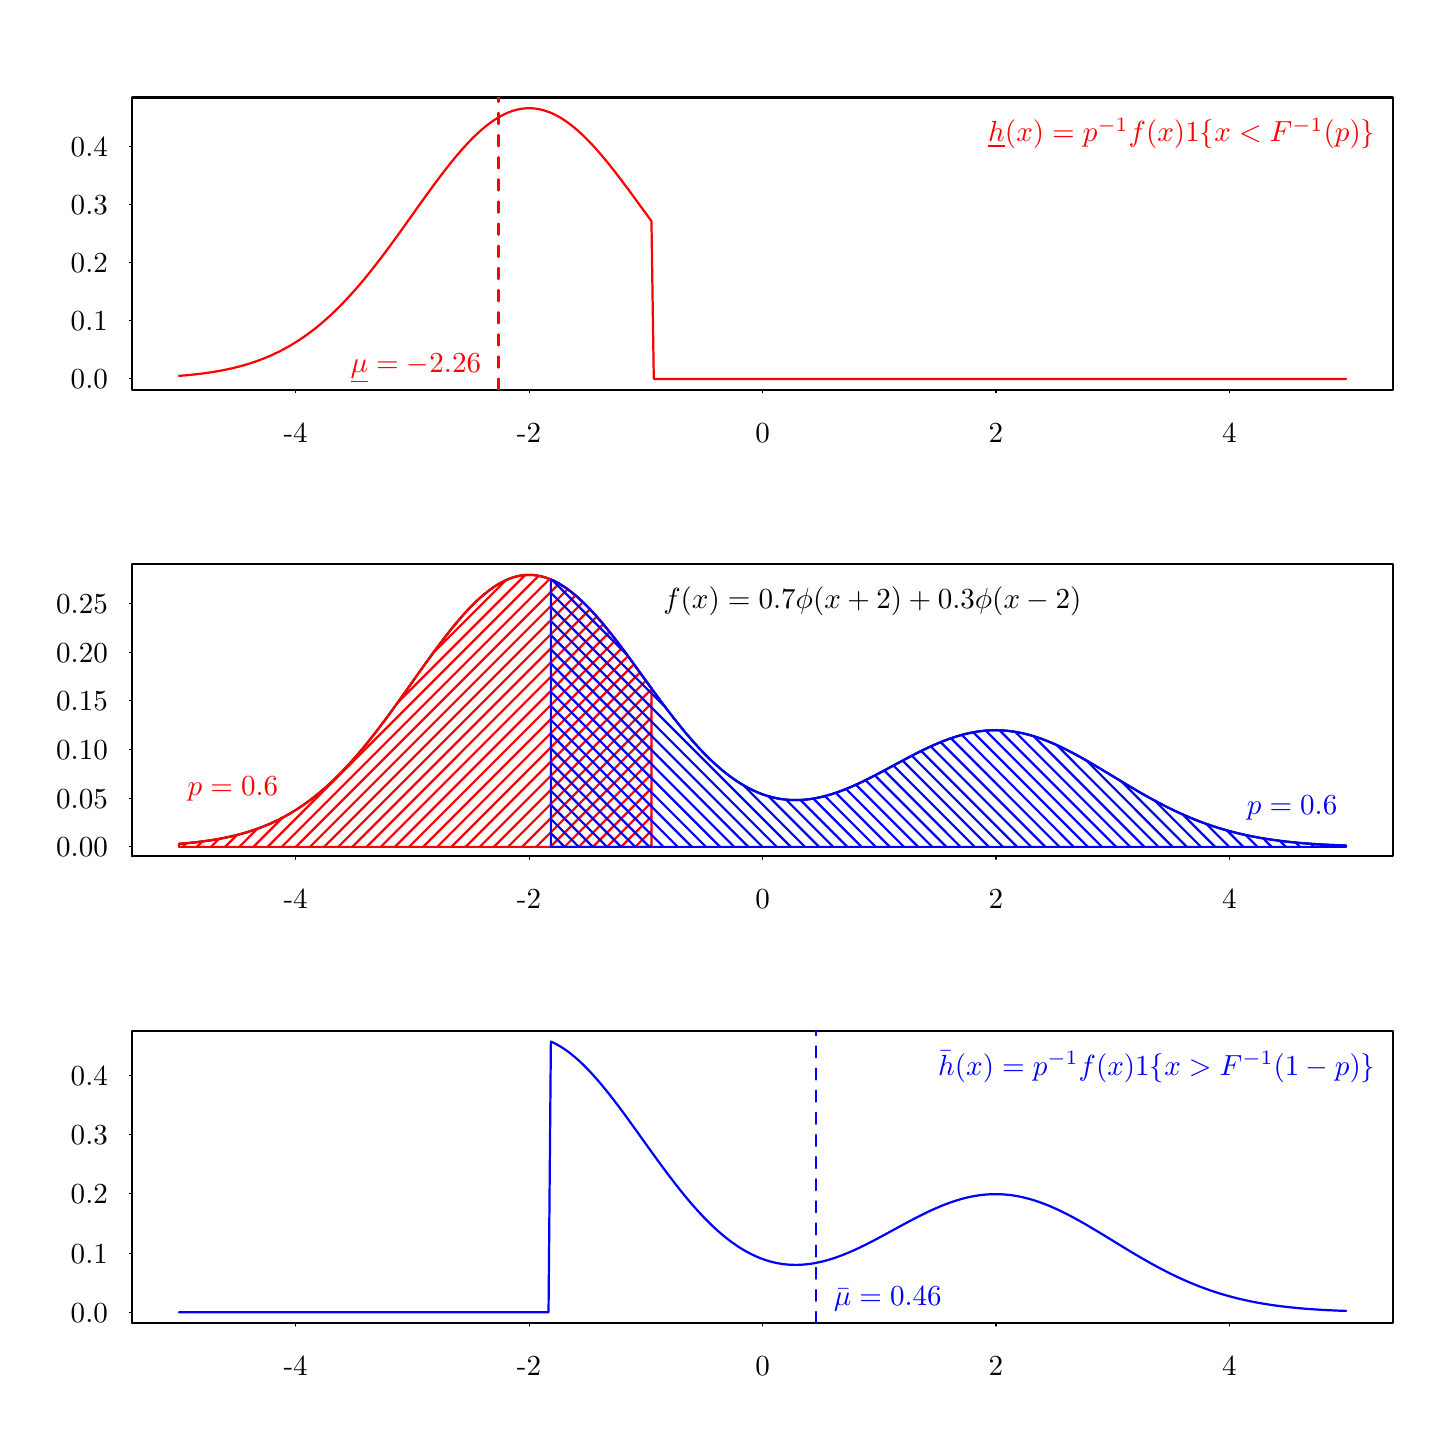
\begin{tikzpicture}[x=1pt,y=1pt]
\definecolor{fillColor}{RGB}{255,255,255}
\path[use as bounding box,fill=fillColor,fill opacity=0.00] (0,0) rectangle (505.89,505.89);
\begin{scope}
\path[clip] ( 37.80,375.06) rectangle (493.29,480.69);
\definecolor{drawColor}{RGB}{255,0,0}

\path[draw=drawColor,line width= 0.8pt,line join=round,line cap=round] ( 54.67,380.06) --
	( 55.52,380.13) --
	( 56.36,380.20) --
	( 57.21,380.27) --
	( 58.05,380.35) --
	( 58.90,380.43) --
	( 59.74,380.52) --
	( 60.59,380.61) --
	( 61.43,380.71) --
	( 62.28,380.81) --
	( 63.12,380.91) --
	( 63.97,381.03) --
	( 64.81,381.14) --
	( 65.66,381.27) --
	( 66.50,381.40) --
	( 67.35,381.53) --
	( 68.19,381.67) --
	( 69.04,381.82) --
	( 69.88,381.98) --
	( 70.73,382.14) --
	( 71.57,382.31) --
	( 72.42,382.49) --
	( 73.26,382.67) --
	( 74.11,382.87) --
	( 74.95,383.07) --
	( 75.80,383.28) --
	( 76.64,383.50) --
	( 77.49,383.73) --
	( 78.34,383.97) --
	( 79.18,384.22) --
	( 80.03,384.48) --
	( 80.87,384.75) --
	( 81.72,385.03) --
	( 82.56,385.32) --
	( 83.41,385.62) --
	( 84.25,385.94) --
	( 85.10,386.27) --
	( 85.94,386.60) --
	( 86.79,386.96) --
	( 87.63,387.32) --
	( 88.48,387.70) --
	( 89.32,388.09) --
	( 90.17,388.50) --
	( 91.01,388.91) --
	( 91.86,389.35) --
	( 92.70,389.79) --
	( 93.55,390.26) --
	( 94.39,390.73) --
	( 95.24,391.23) --
	( 96.08,391.74) --
	( 96.93,392.26) --
	( 97.77,392.80) --
	( 98.62,393.36) --
	( 99.47,393.93) --
	(100.31,394.52) --
	(101.16,395.12) --
	(102.00,395.75) --
	(102.85,396.39) --
	(103.69,397.04) --
	(104.54,397.72) --
	(105.38,398.41) --
	(106.23,399.12) --
	(107.07,399.84) --
	(107.92,400.59) --
	(108.76,401.35) --
	(109.61,402.13) --
	(110.45,402.93) --
	(111.30,403.74) --
	(112.14,404.57) --
	(112.99,405.42) --
	(113.83,406.28) --
	(114.68,407.17) --
	(115.52,408.07) --
	(116.37,408.98) --
	(117.21,409.92) --
	(118.06,410.86) --
	(118.90,411.83) --
	(119.75,412.81) --
	(120.59,413.80) --
	(121.44,414.82) --
	(122.29,415.84) --
	(123.13,416.88) --
	(123.98,417.93) --
	(124.82,419.00) --
	(125.67,420.08) --
	(126.51,421.17) --
	(127.36,422.27) --
	(128.20,423.38) --
	(129.05,424.50) --
	(129.89,425.64) --
	(130.74,426.78) --
	(131.58,427.93) --
	(132.43,429.09) --
	(133.27,430.25) --
	(134.12,431.42) --
	(134.96,432.60) --
	(135.81,433.78) --
	(136.65,434.96) --
	(137.50,436.15) --
	(138.34,437.34) --
	(139.19,438.52) --
	(140.03,439.71) --
	(140.88,440.90) --
	(141.72,442.09) --
	(142.57,443.27) --
	(143.41,444.45) --
	(144.26,445.62) --
	(145.11,446.78) --
	(145.95,447.94) --
	(146.80,449.09) --
	(147.64,450.24) --
	(148.49,451.37) --
	(149.33,452.49) --
	(150.18,453.59) --
	(151.02,454.68) --
	(151.87,455.76) --
	(152.71,456.82) --
	(153.56,457.87) --
	(154.40,458.90) --
	(155.25,459.90) --
	(156.09,460.89) --
	(156.94,461.86) --
	(157.78,462.80) --
	(158.63,463.72) --
	(159.47,464.62) --
	(160.32,465.49) --
	(161.16,466.34) --
	(162.01,467.15) --
	(162.85,467.94) --
	(163.70,468.71) --
	(164.54,469.44) --
	(165.39,470.14) --
	(166.24,470.81) --
	(167.08,471.44) --
	(167.93,472.05) --
	(168.77,472.62) --
	(169.62,473.15) --
	(170.46,473.65) --
	(171.31,474.12) --
	(172.15,474.55) --
	(173.00,474.94) --
	(173.84,475.30) --
	(174.69,475.62) --
	(175.53,475.90) --
	(176.38,476.14) --
	(177.22,476.34) --
	(178.07,476.51) --
	(178.91,476.63) --
	(179.76,476.72) --
	(180.60,476.77) --
	(181.45,476.78) --
	(182.29,476.75) --
	(183.14,476.68) --
	(183.98,476.57) --
	(184.83,476.42) --
	(185.67,476.24) --
	(186.52,476.01) --
	(187.36,475.75) --
	(188.21,475.45) --
	(189.06,475.11) --
	(189.90,474.74) --
	(190.75,474.32) --
	(191.59,473.88) --
	(192.44,473.39) --
	(193.28,472.87) --
	(194.13,472.32) --
	(194.97,471.73) --
	(195.82,471.11) --
	(196.66,470.46) --
	(197.51,469.78) --
	(198.35,469.06) --
	(199.20,468.32) --
	(200.04,467.55) --
	(200.89,466.75) --
	(201.73,465.92) --
	(202.58,465.06) --
	(203.42,464.18) --
	(204.27,463.28) --
	(205.11,462.35) --
	(205.96,461.40) --
	(206.80,460.43) --
	(207.65,459.44) --
	(208.49,458.43) --
	(209.34,457.41) --
	(210.19,456.36) --
	(211.03,455.30) --
	(211.88,454.23) --
	(212.72,453.14) --
	(213.57,452.04) --
	(214.41,450.93) --
	(215.26,449.81) --
	(216.10,448.68) --
	(216.95,447.54) --
	(217.79,446.40) --
	(218.64,445.24) --
	(219.48,444.09) --
	(220.33,442.93) --
	(221.17,441.77) --
	(222.02,440.61) --
	(222.86,439.45) --
	(223.71,438.29) --
	(224.55,437.13) --
	(225.40,435.97) --
	(226.24,378.97) --
	(227.09,378.97) --
	(227.93,378.97) --
	(228.78,378.97) --
	(229.62,378.97) --
	(230.47,378.97) --
	(231.31,378.97) --
	(232.16,378.97) --
	(233.01,378.97) --
	(233.85,378.97) --
	(234.70,378.97) --
	(235.54,378.97) --
	(236.39,378.97) --
	(237.23,378.97) --
	(238.08,378.97) --
	(238.92,378.97) --
	(239.77,378.97) --
	(240.61,378.97) --
	(241.46,378.97) --
	(242.30,378.97) --
	(243.15,378.97) --
	(243.99,378.97) --
	(244.84,378.97) --
	(245.68,378.97) --
	(246.53,378.97) --
	(247.37,378.97) --
	(248.22,378.97) --
	(249.06,378.97) --
	(249.91,378.97) --
	(250.75,378.97) --
	(251.60,378.97) --
	(252.44,378.97) --
	(253.29,378.97) --
	(254.13,378.97) --
	(254.98,378.97) --
	(255.83,378.97) --
	(256.67,378.97) --
	(257.52,378.97) --
	(258.36,378.97) --
	(259.21,378.97) --
	(260.05,378.97) --
	(260.90,378.97) --
	(261.74,378.97) --
	(262.59,378.97) --
	(263.43,378.97) --
	(264.28,378.97) --
	(265.12,378.97) --
	(265.97,378.97) --
	(266.81,378.97) --
	(267.66,378.97) --
	(268.50,378.97) --
	(269.35,378.97) --
	(270.19,378.97) --
	(271.04,378.97) --
	(271.88,378.97) --
	(272.73,378.97) --
	(273.57,378.97) --
	(274.42,378.97) --
	(275.26,378.97) --
	(276.11,378.97) --
	(276.96,378.97) --
	(277.80,378.97) --
	(278.65,378.97) --
	(279.49,378.97) --
	(280.34,378.97) --
	(281.18,378.97) --
	(282.03,378.97) --
	(282.87,378.97) --
	(283.72,378.97) --
	(284.56,378.97) --
	(285.41,378.97) --
	(286.25,378.97) --
	(287.10,378.97) --
	(287.94,378.97) --
	(288.79,378.97) --
	(289.63,378.97) --
	(290.48,378.97) --
	(291.32,378.97) --
	(292.17,378.97) --
	(293.01,378.97) --
	(293.86,378.97) --
	(294.70,378.97) --
	(295.55,378.97) --
	(296.39,378.97) --
	(297.24,378.97) --
	(298.08,378.97) --
	(298.93,378.97) --
	(299.78,378.97) --
	(300.62,378.97) --
	(301.47,378.97) --
	(302.31,378.97) --
	(303.16,378.97) --
	(304.00,378.97) --
	(304.85,378.97) --
	(305.69,378.97) --
	(306.54,378.97) --
	(307.38,378.97) --
	(308.23,378.97) --
	(309.07,378.97) --
	(309.92,378.97) --
	(310.76,378.97) --
	(311.61,378.97) --
	(312.45,378.97) --
	(313.30,378.97) --
	(314.14,378.97) --
	(314.99,378.97) --
	(315.83,378.97) --
	(316.68,378.97) --
	(317.52,378.97) --
	(318.37,378.97) --
	(319.21,378.97) --
	(320.06,378.97) --
	(320.90,378.97) --
	(321.75,378.97) --
	(322.60,378.97) --
	(323.44,378.97) --
	(324.29,378.97) --
	(325.13,378.97) --
	(325.98,378.97) --
	(326.82,378.97) --
	(327.67,378.97) --
	(328.51,378.97) --
	(329.36,378.97) --
	(330.20,378.97) --
	(331.05,378.97) --
	(331.89,378.97) --
	(332.74,378.97) --
	(333.58,378.97) --
	(334.43,378.97) --
	(335.27,378.97) --
	(336.12,378.97) --
	(336.96,378.97) --
	(337.81,378.97) --
	(338.65,378.97) --
	(339.50,378.97) --
	(340.34,378.97) --
	(341.19,378.97) --
	(342.03,378.97) --
	(342.88,378.97) --
	(343.73,378.97) --
	(344.57,378.97) --
	(345.42,378.97) --
	(346.26,378.97) --
	(347.11,378.97) --
	(347.95,378.97) --
	(348.80,378.97) --
	(349.64,378.97) --
	(350.49,378.97) --
	(351.33,378.97) --
	(352.18,378.97) --
	(353.02,378.97) --
	(353.87,378.97) --
	(354.71,378.97) --
	(355.56,378.97) --
	(356.40,378.97) --
	(357.25,378.97) --
	(358.09,378.97) --
	(358.94,378.97) --
	(359.78,378.97) --
	(360.63,378.97) --
	(361.47,378.97) --
	(362.32,378.97) --
	(363.16,378.97) --
	(364.01,378.97) --
	(364.85,378.97) --
	(365.70,378.97) --
	(366.55,378.97) --
	(367.39,378.97) --
	(368.24,378.97) --
	(369.08,378.97) --
	(369.93,378.97) --
	(370.77,378.97) --
	(371.62,378.97) --
	(372.46,378.97) --
	(373.31,378.97) --
	(374.15,378.97) --
	(375.00,378.97) --
	(375.84,378.97) --
	(376.69,378.97) --
	(377.53,378.97) --
	(378.38,378.97) --
	(379.22,378.97) --
	(380.07,378.97) --
	(380.91,378.97) --
	(381.76,378.97) --
	(382.60,378.97) --
	(383.45,378.97) --
	(384.29,378.97) --
	(385.14,378.97) --
	(385.98,378.97) --
	(386.83,378.97) --
	(387.68,378.97) --
	(388.52,378.97) --
	(389.37,378.97) --
	(390.21,378.97) --
	(391.06,378.97) --
	(391.90,378.97) --
	(392.75,378.97) --
	(393.59,378.97) --
	(394.44,378.97) --
	(395.28,378.97) --
	(396.13,378.97) --
	(396.97,378.97) --
	(397.82,378.97) --
	(398.66,378.97) --
	(399.51,378.97) --
	(400.35,378.97) --
	(401.20,378.97) --
	(402.04,378.97) --
	(402.89,378.97) --
	(403.73,378.97) --
	(404.58,378.97) --
	(405.42,378.97) --
	(406.27,378.97) --
	(407.11,378.97) --
	(407.96,378.97) --
	(408.80,378.97) --
	(409.65,378.97) --
	(410.50,378.97) --
	(411.34,378.97) --
	(412.19,378.97) --
	(413.03,378.97) --
	(413.88,378.97) --
	(414.72,378.97) --
	(415.57,378.97) --
	(416.41,378.97) --
	(417.26,378.97) --
	(418.10,378.97) --
	(418.95,378.97) --
	(419.79,378.97) --
	(420.64,378.97) --
	(421.48,378.97) --
	(422.33,378.97) --
	(423.17,378.97) --
	(424.02,378.97) --
	(424.86,378.97) --
	(425.71,378.97) --
	(426.55,378.97) --
	(427.40,378.97) --
	(428.24,378.97) --
	(429.09,378.97) --
	(429.93,378.97) --
	(430.78,378.97) --
	(431.62,378.97) --
	(432.47,378.97) --
	(433.32,378.97) --
	(434.16,378.97) --
	(435.01,378.97) --
	(435.85,378.97) --
	(436.70,378.97) --
	(437.54,378.97) --
	(438.39,378.97) --
	(439.23,378.97) --
	(440.08,378.97) --
	(440.92,378.97) --
	(441.77,378.97) --
	(442.61,378.97) --
	(443.46,378.97) --
	(444.30,378.97) --
	(445.15,378.97) --
	(445.99,378.97) --
	(446.84,378.97) --
	(447.68,378.97) --
	(448.53,378.97) --
	(449.37,378.97) --
	(450.22,378.97) --
	(451.06,378.97) --
	(451.91,378.97) --
	(452.75,378.97) --
	(453.60,378.97) --
	(454.45,378.97) --
	(455.29,378.97) --
	(456.14,378.97) --
	(456.98,378.97) --
	(457.83,378.97) --
	(458.67,378.97) --
	(459.52,378.97) --
	(460.36,378.97) --
	(461.21,378.97) --
	(462.05,378.97) --
	(462.90,378.97) --
	(463.74,378.97) --
	(464.59,378.97) --
	(465.43,378.97) --
	(466.28,378.97) --
	(467.12,378.97) --
	(467.97,378.97) --
	(468.81,378.97) --
	(469.66,378.97) --
	(470.50,378.97) --
	(471.35,378.97) --
	(472.19,378.97) --
	(473.04,378.97) --
	(473.88,378.97) --
	(474.73,378.97) --
	(475.57,378.97) --
	(476.42,378.97);
\end{scope}
\begin{scope}
\path[clip] (  0.00,  0.00) rectangle (505.89,505.89);
\definecolor{drawColor}{RGB}{0,0,0}

\path[draw=drawColor,line width= 0.4pt,line join=round,line cap=round] ( 96.84,375.06) -- (434.25,375.06);

\path[draw=drawColor,line width= 0.4pt,line join=round,line cap=round] ( 96.84,375.06) -- ( 96.84,374.00);

\path[draw=drawColor,line width= 0.4pt,line join=round,line cap=round] (181.19,375.06) -- (181.19,374.00);

\path[draw=drawColor,line width= 0.4pt,line join=round,line cap=round] (265.54,375.06) -- (265.54,374.00);

\path[draw=drawColor,line width= 0.4pt,line join=round,line cap=round] (349.89,375.06) -- (349.89,374.00);

\path[draw=drawColor,line width= 0.4pt,line join=round,line cap=round] (434.25,375.06) -- (434.25,374.00);

\node[text=drawColor,anchor=base,inner sep=0pt, outer sep=0pt, scale=  1.05] at ( 96.84,356.16) {-4};

\node[text=drawColor,anchor=base,inner sep=0pt, outer sep=0pt, scale=  1.05] at (181.19,356.16) {-2};

\node[text=drawColor,anchor=base,inner sep=0pt, outer sep=0pt, scale=  1.05] at (265.54,356.16) {0};

\node[text=drawColor,anchor=base,inner sep=0pt, outer sep=0pt, scale=  1.05] at (349.89,356.16) {2};

\node[text=drawColor,anchor=base,inner sep=0pt, outer sep=0pt, scale=  1.05] at (434.25,356.16) {4};

\path[draw=drawColor,line width= 0.4pt,line join=round,line cap=round] ( 37.80,378.97) -- ( 37.80,463.02);

\path[draw=drawColor,line width= 0.4pt,line join=round,line cap=round] ( 37.80,378.97) -- ( 36.74,378.97);

\path[draw=drawColor,line width= 0.4pt,line join=round,line cap=round] ( 37.80,399.98) -- ( 36.74,399.98);

\path[draw=drawColor,line width= 0.4pt,line join=round,line cap=round] ( 37.80,420.99) -- ( 36.74,420.99);

\path[draw=drawColor,line width= 0.4pt,line join=round,line cap=round] ( 37.80,442.01) -- ( 36.74,442.01);

\path[draw=drawColor,line width= 0.4pt,line join=round,line cap=round] ( 37.80,463.02) -- ( 36.74,463.02);

\node[text=drawColor,anchor=base east,inner sep=0pt, outer sep=0pt, scale=  1.05] at ( 28.98,375.36) {0.0};

\node[text=drawColor,anchor=base east,inner sep=0pt, outer sep=0pt, scale=  1.05] at ( 28.98,396.37) {0.1};

\node[text=drawColor,anchor=base east,inner sep=0pt, outer sep=0pt, scale=  1.05] at ( 28.98,417.38) {0.2};

\node[text=drawColor,anchor=base east,inner sep=0pt, outer sep=0pt, scale=  1.05] at ( 28.98,438.39) {0.3};

\node[text=drawColor,anchor=base east,inner sep=0pt, outer sep=0pt, scale=  1.05] at ( 28.98,459.40) {0.4};

\path[draw=drawColor,line width= 0.8pt,line join=round,line cap=round] ( 37.80,375.06) --
	(493.29,375.06) --
	(493.29,480.69) --
	( 37.80,480.69) --
	( 37.80,375.06);
\end{scope}
\begin{scope}
\path[clip] ( 37.80,375.06) rectangle (493.29,480.69);
\definecolor{drawColor}{RGB}{255,0,0}

\node[text=drawColor,anchor=base east,inner sep=0pt, outer sep=0pt, scale=  1.05] at (486.99,464.59) {$\underline{h}(x) = p^{-1}f(x) 1\{x < F^{-1}(p)\}$};

\path[draw=drawColor,line width= 0.8pt,dash pattern=on 4pt off 4pt ,line join=round,line cap=round] (170.15,375.06) -- (170.15,480.69);

\node[text=drawColor,anchor=base east,inner sep=0pt, outer sep=0pt, scale=  1.05] at (163.85,381.45) {$\underline{\mu} = -2.26$};
\end{scope}
\begin{scope}
\path[clip] ( 37.80,206.43) rectangle (493.29,312.06);
\definecolor{drawColor}{RGB}{0,0,0}

\path[draw=drawColor,line width= 0.8pt,line join=round,line cap=round] ( 54.67,210.97) --
	( 55.52,211.03) --
	( 56.36,211.10) --
	( 57.21,211.18) --
	( 58.05,211.26) --
	( 58.90,211.34) --
	( 59.74,211.43) --
	( 60.59,211.52) --
	( 61.43,211.62) --
	( 62.28,211.72) --
	( 63.12,211.83) --
	( 63.97,211.94) --
	( 64.81,212.06) --
	( 65.66,212.18) --
	( 66.50,212.31) --
	( 67.35,212.45) --
	( 68.19,212.59) --
	( 69.04,212.74) --
	( 69.88,212.89) --
	( 70.73,213.06) --
	( 71.57,213.23) --
	( 72.42,213.41) --
	( 73.26,213.59) --
	( 74.11,213.79) --
	( 74.95,213.99) --
	( 75.80,214.20) --
	( 76.64,214.42) --
	( 77.49,214.65) --
	( 78.34,214.90) --
	( 79.18,215.15) --
	( 80.03,215.41) --
	( 80.87,215.68) --
	( 81.72,215.96) --
	( 82.56,216.25) --
	( 83.41,216.56) --
	( 84.25,216.87) --
	( 85.10,217.20) --
	( 85.94,217.54) --
	( 86.79,217.90) --
	( 87.63,218.26) --
	( 88.48,218.64) --
	( 89.32,219.04) --
	( 90.17,219.44) --
	( 91.01,219.86) --
	( 91.86,220.30) --
	( 92.70,220.75) --
	( 93.55,221.21) --
	( 94.39,221.69) --
	( 95.24,222.19) --
	( 96.08,222.70) --
	( 96.93,223.23) --
	( 97.77,223.77) --
	( 98.62,224.33) --
	( 99.47,224.90) --
	(100.31,225.49) --
	(101.16,226.10) --
	(102.00,226.73) --
	(102.85,227.37) --
	(103.69,228.03) --
	(104.54,228.71) --
	(105.38,229.40) --
	(106.23,230.12) --
	(107.07,230.85) --
	(107.92,231.59) --
	(108.76,232.36) --
	(109.61,233.14) --
	(110.45,233.94) --
	(111.30,234.76) --
	(112.14,235.59) --
	(112.99,236.45) --
	(113.83,237.32) --
	(114.68,238.20) --
	(115.52,239.11) --
	(116.37,240.03) --
	(117.21,240.97) --
	(118.06,241.92) --
	(118.90,242.89) --
	(119.75,243.87) --
	(120.59,244.87) --
	(121.44,245.89) --
	(122.29,246.92) --
	(123.13,247.96) --
	(123.98,249.02) --
	(124.82,250.09) --
	(125.67,251.17) --
	(126.51,252.27) --
	(127.36,253.38) --
	(128.20,254.50) --
	(129.05,255.62) --
	(129.89,256.76) --
	(130.74,257.91) --
	(131.58,259.07) --
	(132.43,260.23) --
	(133.27,261.40) --
	(134.12,262.58) --
	(134.96,263.76) --
	(135.81,264.94) --
	(136.65,266.13) --
	(137.50,267.32) --
	(138.34,268.52) --
	(139.19,269.71) --
	(140.03,270.91) --
	(140.88,272.10) --
	(141.72,273.29) --
	(142.57,274.48) --
	(143.41,275.66) --
	(144.26,276.84) --
	(145.11,278.01) --
	(145.95,279.18) --
	(146.80,280.33) --
	(147.64,281.48) --
	(148.49,282.61) --
	(149.33,283.74) --
	(150.18,284.85) --
	(151.02,285.95) --
	(151.87,287.03) --
	(152.71,288.10) --
	(153.56,289.15) --
	(154.40,290.18) --
	(155.25,291.19) --
	(156.09,292.19) --
	(156.94,293.16) --
	(157.78,294.11) --
	(158.63,295.03) --
	(159.47,295.93) --
	(160.32,296.81) --
	(161.16,297.66) --
	(162.01,298.48) --
	(162.85,299.27) --
	(163.70,300.04) --
	(164.54,300.77) --
	(165.39,301.47) --
	(166.24,302.15) --
	(167.08,302.79) --
	(167.93,303.39) --
	(168.77,303.97) --
	(169.62,304.51) --
	(170.46,305.01) --
	(171.31,305.48) --
	(172.15,305.91) --
	(173.00,306.30) --
	(173.84,306.66) --
	(174.69,306.98) --
	(175.53,307.26) --
	(176.38,307.50) --
	(177.22,307.71) --
	(178.07,307.88) --
	(178.91,308.00) --
	(179.76,308.09) --
	(180.60,308.14) --
	(181.45,308.15) --
	(182.29,308.12) --
	(183.14,308.05) --
	(183.98,307.94) --
	(184.83,307.79) --
	(185.67,307.60) --
	(186.52,307.38) --
	(187.36,307.11) --
	(188.21,306.81) --
	(189.06,306.47) --
	(189.90,306.10) --
	(190.75,305.68) --
	(191.59,305.23) --
	(192.44,304.75) --
	(193.28,304.22) --
	(194.13,303.67) --
	(194.97,303.08) --
	(195.82,302.46) --
	(196.66,301.80) --
	(197.51,301.12) --
	(198.35,300.40) --
	(199.20,299.65) --
	(200.04,298.87) --
	(200.89,298.07) --
	(201.73,297.24) --
	(202.58,296.38) --
	(203.42,295.49) --
	(204.27,294.59) --
	(205.11,293.65) --
	(205.96,292.70) --
	(206.80,291.73) --
	(207.65,290.73) --
	(208.49,289.72) --
	(209.34,288.68) --
	(210.19,287.63) --
	(211.03,286.57) --
	(211.88,285.49) --
	(212.72,284.40) --
	(213.57,283.29) --
	(214.41,282.18) --
	(215.26,281.05) --
	(216.10,279.91) --
	(216.95,278.77) --
	(217.79,277.62) --
	(218.64,276.46) --
	(219.48,275.30) --
	(220.33,274.14) --
	(221.17,272.97) --
	(222.02,271.81) --
	(222.86,270.64) --
	(223.71,269.47) --
	(224.55,268.31) --
	(225.40,267.15) --
	(226.24,265.99) --
	(227.09,264.84) --
	(227.93,263.69) --
	(228.78,262.55) --
	(229.62,261.42) --
	(230.47,260.29) --
	(231.31,259.18) --
	(232.16,258.08) --
	(233.01,256.98) --
	(233.85,255.90) --
	(234.70,254.83) --
	(235.54,253.78) --
	(236.39,252.74) --
	(237.23,251.71) --
	(238.08,250.70) --
	(238.92,249.71) --
	(239.77,248.73) --
	(240.61,247.77) --
	(241.46,246.82) --
	(242.30,245.90) --
	(243.15,244.99) --
	(243.99,244.10) --
	(244.84,243.24) --
	(245.68,242.39) --
	(246.53,241.56) --
	(247.37,240.76) --
	(248.22,239.97) --
	(249.06,239.21) --
	(249.91,238.47) --
	(250.75,237.75) --
	(251.60,237.05) --
	(252.44,236.38) --
	(253.29,235.73) --
	(254.13,235.10) --
	(254.98,234.49) --
	(255.83,233.91) --
	(256.67,233.35) --
	(257.52,232.81) --
	(258.36,232.30) --
	(259.21,231.81) --
	(260.05,231.34) --
	(260.90,230.90) --
	(261.74,230.48) --
	(262.59,230.08) --
	(263.43,229.70) --
	(264.28,229.35) --
	(265.12,229.03) --
	(265.97,228.72) --
	(266.81,228.44) --
	(267.66,228.18) --
	(268.50,227.94) --
	(269.35,227.73) --
	(270.19,227.54) --
	(271.04,227.37) --
	(271.88,227.22) --
	(272.73,227.09) --
	(273.57,226.99) --
	(274.42,226.90) --
	(275.26,226.84) --
	(276.11,226.80) --
	(276.96,226.78) --
	(277.80,226.77) --
	(278.65,226.79) --
	(279.49,226.83) --
	(280.34,226.88) --
	(281.18,226.96) --
	(282.03,227.05) --
	(282.87,227.16) --
	(283.72,227.29) --
	(284.56,227.44) --
	(285.41,227.60) --
	(286.25,227.78) --
	(287.10,227.97) --
	(287.94,228.18) --
	(288.79,228.41) --
	(289.63,228.65) --
	(290.48,228.91) --
	(291.32,229.18) --
	(292.17,229.46) --
	(293.01,229.76) --
	(293.86,230.07) --
	(294.70,230.39) --
	(295.55,230.72) --
	(296.39,231.07) --
	(297.24,231.42) --
	(298.08,231.79) --
	(298.93,232.16) --
	(299.78,232.55) --
	(300.62,232.94) --
	(301.47,233.34) --
	(302.31,233.75) --
	(303.16,234.16) --
	(304.00,234.59) --
	(304.85,235.01) --
	(305.69,235.45) --
	(306.54,235.89) --
	(307.38,236.33) --
	(308.23,236.78) --
	(309.07,237.23) --
	(309.92,237.68) --
	(310.76,238.13) --
	(311.61,238.59) --
	(312.45,239.05) --
	(313.30,239.50) --
	(314.14,239.96) --
	(314.99,240.41) --
	(315.83,240.87) --
	(316.68,241.32) --
	(317.52,241.77) --
	(318.37,242.22) --
	(319.21,242.66) --
	(320.06,243.10) --
	(320.90,243.53) --
	(321.75,243.96) --
	(322.60,244.38) --
	(323.44,244.80) --
	(324.29,245.21) --
	(325.13,245.61) --
	(325.98,246.00) --
	(326.82,246.39) --
	(327.67,246.76) --
	(328.51,247.13) --
	(329.36,247.48) --
	(330.20,247.83) --
	(331.05,248.16) --
	(331.89,248.49) --
	(332.74,248.80) --
	(333.58,249.09) --
	(334.43,249.38) --
	(335.27,249.65) --
	(336.12,249.91) --
	(336.96,250.16) --
	(337.81,250.39) --
	(338.65,250.61) --
	(339.50,250.81) --
	(340.34,251.00) --
	(341.19,251.17) --
	(342.03,251.33) --
	(342.88,251.47) --
	(343.73,251.60) --
	(344.57,251.71) --
	(345.42,251.80) --
	(346.26,251.88) --
	(347.11,251.94) --
	(347.95,251.98) --
	(348.80,252.01) --
	(349.64,252.02) --
	(350.49,252.01) --
	(351.33,251.99) --
	(352.18,251.95) --
	(353.02,251.89) --
	(353.87,251.82) --
	(354.71,251.73) --
	(355.56,251.63) --
	(356.40,251.51) --
	(357.25,251.37) --
	(358.09,251.21) --
	(358.94,251.04) --
	(359.78,250.86) --
	(360.63,250.66) --
	(361.47,250.44) --
	(362.32,250.21) --
	(363.16,249.96) --
	(364.01,249.70) --
	(364.85,249.43) --
	(365.70,249.14) --
	(366.55,248.84) --
	(367.39,248.52) --
	(368.24,248.19) --
	(369.08,247.85) --
	(369.93,247.50) --
	(370.77,247.13) --
	(371.62,246.76) --
	(372.46,246.37) --
	(373.31,245.98) --
	(374.15,245.57) --
	(375.00,245.15) --
	(375.84,244.73) --
	(376.69,244.29) --
	(377.53,243.85) --
	(378.38,243.40) --
	(379.22,242.94) --
	(380.07,242.48) --
	(380.91,242.01) --
	(381.76,241.53) --
	(382.60,241.05) --
	(383.45,240.56) --
	(384.29,240.07) --
	(385.14,239.58) --
	(385.98,239.08) --
	(386.83,238.57) --
	(387.68,238.07) --
	(388.52,237.56) --
	(389.37,237.05) --
	(390.21,236.54) --
	(391.06,236.03) --
	(391.90,235.52) --
	(392.75,235.01) --
	(393.59,234.50) --
	(394.44,233.98) --
	(395.28,233.48) --
	(396.13,232.97) --
	(396.97,232.46) --
	(397.82,231.96) --
	(398.66,231.46) --
	(399.51,230.96) --
	(400.35,230.46) --
	(401.20,229.97) --
	(402.04,229.48) --
	(402.89,229.00) --
	(403.73,228.52) --
	(404.58,228.04) --
	(405.42,227.57) --
	(406.27,227.11) --
	(407.11,226.65) --
	(407.96,226.20) --
	(408.80,225.75) --
	(409.65,225.31) --
	(410.50,224.87) --
	(411.34,224.45) --
	(412.19,224.02) --
	(413.03,223.61) --
	(413.88,223.20) --
	(414.72,222.80) --
	(415.57,222.40) --
	(416.41,222.02) --
	(417.26,221.64) --
	(418.10,221.26) --
	(418.95,220.90) --
	(419.79,220.54) --
	(420.64,220.19) --
	(421.48,219.85) --
	(422.33,219.51) --
	(423.17,219.18) --
	(424.02,218.86) --
	(424.86,218.55) --
	(425.71,218.24) --
	(426.55,217.95) --
	(427.40,217.66) --
	(428.24,217.37) --
	(429.09,217.10) --
	(429.93,216.83) --
	(430.78,216.57) --
	(431.62,216.32) --
	(432.47,216.07) --
	(433.32,215.83) --
	(434.16,215.60) --
	(435.01,215.37) --
	(435.85,215.15) --
	(436.70,214.94) --
	(437.54,214.73) --
	(438.39,214.53) --
	(439.23,214.34) --
	(440.08,214.16) --
	(440.92,213.98) --
	(441.77,213.80) --
	(442.61,213.63) --
	(443.46,213.47) --
	(444.30,213.31) --
	(445.15,213.16) --
	(445.99,213.02) --
	(446.84,212.87) --
	(447.68,212.74) --
	(448.53,212.61) --
	(449.37,212.48) --
	(450.22,212.36) --
	(451.06,212.25) --
	(451.91,212.13) --
	(452.75,212.03) --
	(453.60,211.92) --
	(454.45,211.82) --
	(455.29,211.73) --
	(456.14,211.64) --
	(456.98,211.55) --
	(457.83,211.47) --
	(458.67,211.39) --
	(459.52,211.31) --
	(460.36,211.24) --
	(461.21,211.17) --
	(462.05,211.10) --
	(462.90,211.04) --
	(463.74,210.98) --
	(464.59,210.92) --
	(465.43,210.86) --
	(466.28,210.81) --
	(467.12,210.76) --
	(467.97,210.71) --
	(468.81,210.67) --
	(469.66,210.62) --
	(470.50,210.58) --
	(471.35,210.54) --
	(472.19,210.50) --
	(473.04,210.47) --
	(473.88,210.43) --
	(474.73,210.40) --
	(475.57,210.37) --
	(476.42,210.34);
\end{scope}
\begin{scope}
\path[clip] (  0.00,  0.00) rectangle (505.89,505.89);
\definecolor{drawColor}{RGB}{0,0,0}

\path[draw=drawColor,line width= 0.4pt,line join=round,line cap=round] ( 96.84,206.43) -- (434.25,206.43);

\path[draw=drawColor,line width= 0.4pt,line join=round,line cap=round] ( 96.84,206.43) -- ( 96.84,205.37);

\path[draw=drawColor,line width= 0.4pt,line join=round,line cap=round] (181.19,206.43) -- (181.19,205.37);

\path[draw=drawColor,line width= 0.4pt,line join=round,line cap=round] (265.54,206.43) -- (265.54,205.37);

\path[draw=drawColor,line width= 0.4pt,line join=round,line cap=round] (349.89,206.43) -- (349.89,205.37);

\path[draw=drawColor,line width= 0.4pt,line join=round,line cap=round] (434.25,206.43) -- (434.25,205.37);

\node[text=drawColor,anchor=base,inner sep=0pt, outer sep=0pt, scale=  1.05] at ( 96.84,187.53) {-4};

\node[text=drawColor,anchor=base,inner sep=0pt, outer sep=0pt, scale=  1.05] at (181.19,187.53) {-2};

\node[text=drawColor,anchor=base,inner sep=0pt, outer sep=0pt, scale=  1.05] at (265.54,187.53) {0};

\node[text=drawColor,anchor=base,inner sep=0pt, outer sep=0pt, scale=  1.05] at (349.89,187.53) {2};

\node[text=drawColor,anchor=base,inner sep=0pt, outer sep=0pt, scale=  1.05] at (434.25,187.53) {4};

\path[draw=drawColor,line width= 0.4pt,line join=round,line cap=round] ( 37.80,209.87) -- ( 37.80,297.84);

\path[draw=drawColor,line width= 0.4pt,line join=round,line cap=round] ( 37.80,209.87) -- ( 36.74,209.87);

\path[draw=drawColor,line width= 0.4pt,line join=round,line cap=round] ( 37.80,227.47) -- ( 36.74,227.47);

\path[draw=drawColor,line width= 0.4pt,line join=round,line cap=round] ( 37.80,245.06) -- ( 36.74,245.06);

\path[draw=drawColor,line width= 0.4pt,line join=round,line cap=round] ( 37.80,262.65) -- ( 36.74,262.65);

\path[draw=drawColor,line width= 0.4pt,line join=round,line cap=round] ( 37.80,280.25) -- ( 36.74,280.25);

\path[draw=drawColor,line width= 0.4pt,line join=round,line cap=round] ( 37.80,297.84) -- ( 36.74,297.84);

\node[text=drawColor,anchor=base east,inner sep=0pt, outer sep=0pt, scale=  1.05] at ( 28.98,206.26) {0.00};

\node[text=drawColor,anchor=base east,inner sep=0pt, outer sep=0pt, scale=  1.05] at ( 28.98,223.85) {0.05};

\node[text=drawColor,anchor=base east,inner sep=0pt, outer sep=0pt, scale=  1.05] at ( 28.98,241.44) {0.10};

\node[text=drawColor,anchor=base east,inner sep=0pt, outer sep=0pt, scale=  1.05] at ( 28.98,259.04) {0.15};

\node[text=drawColor,anchor=base east,inner sep=0pt, outer sep=0pt, scale=  1.05] at ( 28.98,276.63) {0.20};

\node[text=drawColor,anchor=base east,inner sep=0pt, outer sep=0pt, scale=  1.05] at ( 28.98,294.22) {0.25};

\path[draw=drawColor,line width= 0.8pt,line join=round,line cap=round] ( 37.80,206.43) --
	(493.29,206.43) --
	(493.29,312.06) --
	( 37.80,312.06) --
	( 37.80,206.43);
\end{scope}
\begin{scope}
\path[clip] ( 37.80,206.43) rectangle (493.29,312.06);
\definecolor{drawColor}{RGB}{255,0,0}

\path[draw=drawColor,line width= 0.8pt,line join=round,line cap=round] ( 56.02,209.87) -- ( 57.34,211.19);

\path[draw=drawColor,line width= 0.8pt,line join=round,line cap=round] ( 61.13,209.87) -- ( 63.08,211.82);

\path[draw=drawColor,line width= 0.8pt,line join=round,line cap=round] ( 66.24,209.87) -- ( 69.12,212.75);

\path[draw=drawColor,line width= 0.8pt,line join=round,line cap=round] ( 71.36,209.87) -- ( 75.64,214.16);

\path[draw=drawColor,line width= 0.8pt,line join=round,line cap=round] ( 76.47,209.87) -- ( 83.00,216.41);

\path[draw=drawColor,line width= 0.8pt,line join=round,line cap=round] (146.45,279.86) -- (172.80,306.21);

\path[draw=drawColor,line width= 0.8pt,line join=round,line cap=round] ( 81.58,209.87) -- ( 92.16,220.46);

\path[draw=drawColor,line width= 0.8pt,line join=round,line cap=round] (133.71,262.01) -- (179.79,308.09);

\path[draw=drawColor,line width= 0.8pt,line join=round,line cap=round] ( 86.69,209.87) -- (184.64,307.82);

\path[draw=drawColor,line width= 0.8pt,line join=round,line cap=round] ( 91.80,209.87) -- (188.58,306.66);

\path[draw=drawColor,line width= 0.8pt,line join=round,line cap=round] ( 96.91,209.87) -- (192.02,304.99);

\path[draw=drawColor,line width= 0.8pt,line join=round,line cap=round] (102.02,209.87) -- (195.12,302.97);

\path[draw=drawColor,line width= 0.8pt,line join=round,line cap=round] (107.13,209.87) -- (197.97,300.72);

\path[draw=drawColor,line width= 0.8pt,line join=round,line cap=round] (112.24,209.87) -- (200.65,298.29);

\path[draw=drawColor,line width= 0.8pt,line join=round,line cap=round] (117.35,209.87) -- (203.20,295.73);

\path[draw=drawColor,line width= 0.8pt,line join=round,line cap=round] (122.46,209.87) -- (205.64,293.06);

\path[draw=drawColor,line width= 0.8pt,line join=round,line cap=round] (127.57,209.87) -- (208.00,290.31);

\path[draw=drawColor,line width= 0.8pt,line join=round,line cap=round] (132.68,209.87) -- (210.30,287.49);

\path[draw=drawColor,line width= 0.8pt,line join=round,line cap=round] (137.79,209.87) -- (212.54,284.63);

\path[draw=drawColor,line width= 0.8pt,line join=round,line cap=round] (142.90,209.87) -- (214.75,281.72);

\path[draw=drawColor,line width= 0.8pt,line join=round,line cap=round] (148.01,209.87) -- (216.93,278.79);

\path[draw=drawColor,line width= 0.8pt,line join=round,line cap=round] (153.12,209.87) -- (219.09,275.84);

\path[draw=drawColor,line width= 0.8pt,line join=round,line cap=round] (158.23,209.87) -- (221.24,272.88);

\path[draw=drawColor,line width= 0.8pt,line join=round,line cap=round] (163.34,209.87) -- (223.39,269.92);

\path[draw=drawColor,line width= 0.8pt,line join=round,line cap=round] (168.45,209.87) -- (225.40,266.82);

\path[draw=drawColor,line width= 0.8pt,line join=round,line cap=round] (173.56,209.87) -- (225.40,261.71);

\path[draw=drawColor,line width= 0.8pt,line join=round,line cap=round] (178.67,209.87) -- (225.40,256.60);

\path[draw=drawColor,line width= 0.8pt,line join=round,line cap=round] (183.78,209.87) -- (225.40,251.49);

\path[draw=drawColor,line width= 0.8pt,line join=round,line cap=round] (188.89,209.87) -- (225.40,246.38);

\path[draw=drawColor,line width= 0.8pt,line join=round,line cap=round] (194.00,209.87) -- (225.40,241.27);

\path[draw=drawColor,line width= 0.8pt,line join=round,line cap=round] (199.11,209.87) -- (225.40,236.16);

\path[draw=drawColor,line width= 0.8pt,line join=round,line cap=round] (204.22,209.87) -- (225.40,231.05);

\path[draw=drawColor,line width= 0.8pt,line join=round,line cap=round] (209.33,209.87) -- (225.40,225.94);

\path[draw=drawColor,line width= 0.8pt,line join=round,line cap=round] (214.44,209.87) -- (225.40,220.83);

\path[draw=drawColor,line width= 0.8pt,line join=round,line cap=round] (219.55,209.87) -- (225.40,215.72);

\path[draw=drawColor,line width= 0.8pt,line join=round,line cap=round] (224.66,209.87) -- (225.40,210.61);

\path[draw=drawColor,line width= 0.8pt,line join=round,line cap=round] ( 54.67,209.87) --
	( 55.52,209.87) --
	( 56.36,209.87) --
	( 57.21,209.87) --
	( 58.05,209.87) --
	( 58.90,209.87) --
	( 59.74,209.87) --
	( 60.59,209.87) --
	( 61.43,209.87) --
	( 62.28,209.87) --
	( 63.12,209.87) --
	( 63.97,209.87) --
	( 64.81,209.87) --
	( 65.66,209.87) --
	( 66.50,209.87) --
	( 67.35,209.87) --
	( 68.19,209.87) --
	( 69.04,209.87) --
	( 69.88,209.87) --
	( 70.73,209.87) --
	( 71.57,209.87) --
	( 72.42,209.87) --
	( 73.26,209.87) --
	( 74.11,209.87) --
	( 74.95,209.87) --
	( 75.80,209.87) --
	( 76.64,209.87) --
	( 77.49,209.87) --
	( 78.34,209.87) --
	( 79.18,209.87) --
	( 80.03,209.87) --
	( 80.87,209.87) --
	( 81.72,209.87) --
	( 82.56,209.87) --
	( 83.41,209.87) --
	( 84.25,209.87) --
	( 85.10,209.87) --
	( 85.94,209.87) --
	( 86.79,209.87) --
	( 87.63,209.87) --
	( 88.48,209.87) --
	( 89.32,209.87) --
	( 90.17,209.87) --
	( 91.01,209.87) --
	( 91.86,209.87) --
	( 92.70,209.87) --
	( 93.55,209.87) --
	( 94.39,209.87) --
	( 95.24,209.87) --
	( 96.08,209.87) --
	( 96.93,209.87) --
	( 97.77,209.87) --
	( 98.62,209.87) --
	( 99.47,209.87) --
	(100.31,209.87) --
	(101.16,209.87) --
	(102.00,209.87) --
	(102.85,209.87) --
	(103.69,209.87) --
	(104.54,209.87) --
	(105.38,209.87) --
	(106.23,209.87) --
	(107.07,209.87) --
	(107.92,209.87) --
	(108.76,209.87) --
	(109.61,209.87) --
	(110.45,209.87) --
	(111.30,209.87) --
	(112.14,209.87) --
	(112.99,209.87) --
	(113.83,209.87) --
	(114.68,209.87) --
	(115.52,209.87) --
	(116.37,209.87) --
	(117.21,209.87) --
	(118.06,209.87) --
	(118.90,209.87) --
	(119.75,209.87) --
	(120.59,209.87) --
	(121.44,209.87) --
	(122.29,209.87) --
	(123.13,209.87) --
	(123.98,209.87) --
	(124.82,209.87) --
	(125.67,209.87) --
	(126.51,209.87) --
	(127.36,209.87) --
	(128.20,209.87) --
	(129.05,209.87) --
	(129.89,209.87) --
	(130.74,209.87) --
	(131.58,209.87) --
	(132.43,209.87) --
	(133.27,209.87) --
	(134.12,209.87) --
	(134.96,209.87) --
	(135.81,209.87) --
	(136.65,209.87) --
	(137.50,209.87) --
	(138.34,209.87) --
	(139.19,209.87) --
	(140.03,209.87) --
	(140.88,209.87) --
	(141.72,209.87) --
	(142.57,209.87) --
	(143.41,209.87) --
	(144.26,209.87) --
	(145.11,209.87) --
	(145.95,209.87) --
	(146.80,209.87) --
	(147.64,209.87) --
	(148.49,209.87) --
	(149.33,209.87) --
	(150.18,209.87) --
	(151.02,209.87) --
	(151.87,209.87) --
	(152.71,209.87) --
	(153.56,209.87) --
	(154.40,209.87) --
	(155.25,209.87) --
	(156.09,209.87) --
	(156.94,209.87) --
	(157.78,209.87) --
	(158.63,209.87) --
	(159.47,209.87) --
	(160.32,209.87) --
	(161.16,209.87) --
	(162.01,209.87) --
	(162.85,209.87) --
	(163.70,209.87) --
	(164.54,209.87) --
	(165.39,209.87) --
	(166.24,209.87) --
	(167.08,209.87) --
	(167.93,209.87) --
	(168.77,209.87) --
	(169.62,209.87) --
	(170.46,209.87) --
	(171.31,209.87) --
	(172.15,209.87) --
	(173.00,209.87) --
	(173.84,209.87) --
	(174.69,209.87) --
	(175.53,209.87) --
	(176.38,209.87) --
	(177.22,209.87) --
	(178.07,209.87) --
	(178.91,209.87) --
	(179.76,209.87) --
	(180.60,209.87) --
	(181.45,209.87) --
	(182.29,209.87) --
	(183.14,209.87) --
	(183.98,209.87) --
	(184.83,209.87) --
	(185.67,209.87) --
	(186.52,209.87) --
	(187.36,209.87) --
	(188.21,209.87) --
	(189.06,209.87) --
	(189.90,209.87) --
	(190.75,209.87) --
	(191.59,209.87) --
	(192.44,209.87) --
	(193.28,209.87) --
	(194.13,209.87) --
	(194.97,209.87) --
	(195.82,209.87) --
	(196.66,209.87) --
	(197.51,209.87) --
	(198.35,209.87) --
	(199.20,209.87) --
	(200.04,209.87) --
	(200.89,209.87) --
	(201.73,209.87) --
	(202.58,209.87) --
	(203.42,209.87) --
	(204.27,209.87) --
	(205.11,209.87) --
	(205.96,209.87) --
	(206.80,209.87) --
	(207.65,209.87) --
	(208.49,209.87) --
	(209.34,209.87) --
	(210.19,209.87) --
	(211.03,209.87) --
	(211.88,209.87) --
	(212.72,209.87) --
	(213.57,209.87) --
	(214.41,209.87) --
	(215.26,209.87) --
	(216.10,209.87) --
	(216.95,209.87) --
	(217.79,209.87) --
	(218.64,209.87) --
	(219.48,209.87) --
	(220.33,209.87) --
	(221.17,209.87) --
	(222.02,209.87) --
	(222.86,209.87) --
	(223.71,209.87) --
	(224.55,209.87) --
	(225.40,209.87) --
	(225.40,267.15) --
	(224.55,268.31) --
	(223.71,269.47) --
	(222.86,270.64) --
	(222.02,271.81) --
	(221.17,272.97) --
	(220.33,274.14) --
	(219.48,275.30) --
	(218.64,276.46) --
	(217.79,277.62) --
	(216.95,278.77) --
	(216.10,279.91) --
	(215.26,281.05) --
	(214.41,282.18) --
	(213.57,283.29) --
	(212.72,284.40) --
	(211.88,285.49) --
	(211.03,286.57) --
	(210.19,287.63) --
	(209.34,288.68) --
	(208.49,289.72) --
	(207.65,290.73) --
	(206.80,291.73) --
	(205.96,292.70) --
	(205.11,293.65) --
	(204.27,294.59) --
	(203.42,295.49) --
	(202.58,296.38) --
	(201.73,297.24) --
	(200.89,298.07) --
	(200.04,298.87) --
	(199.20,299.65) --
	(198.35,300.40) --
	(197.51,301.12) --
	(196.66,301.80) --
	(195.82,302.46) --
	(194.97,303.08) --
	(194.13,303.67) --
	(193.28,304.22) --
	(192.44,304.75) --
	(191.59,305.23) --
	(190.75,305.68) --
	(189.90,306.10) --
	(189.06,306.47) --
	(188.21,306.81) --
	(187.36,307.11) --
	(186.52,307.38) --
	(185.67,307.60) --
	(184.83,307.79) --
	(183.98,307.94) --
	(183.14,308.05) --
	(182.29,308.12) --
	(181.45,308.15) --
	(180.60,308.14) --
	(179.76,308.09) --
	(178.91,308.00) --
	(178.07,307.88) --
	(177.22,307.71) --
	(176.38,307.50) --
	(175.53,307.26) --
	(174.69,306.98) --
	(173.84,306.66) --
	(173.00,306.30) --
	(172.15,305.91) --
	(171.31,305.48) --
	(170.46,305.01) --
	(169.62,304.51) --
	(168.77,303.97) --
	(167.93,303.39) --
	(167.08,302.79) --
	(166.24,302.15) --
	(165.39,301.47) --
	(164.54,300.77) --
	(163.70,300.04) --
	(162.85,299.27) --
	(162.01,298.48) --
	(161.16,297.66) --
	(160.32,296.81) --
	(159.47,295.93) --
	(158.63,295.03) --
	(157.78,294.11) --
	(156.94,293.16) --
	(156.09,292.19) --
	(155.25,291.19) --
	(154.40,290.18) --
	(153.56,289.15) --
	(152.71,288.10) --
	(151.87,287.03) --
	(151.02,285.95) --
	(150.18,284.85) --
	(149.33,283.74) --
	(148.49,282.61) --
	(147.64,281.48) --
	(146.80,280.33) --
	(145.95,279.18) --
	(145.11,278.01) --
	(144.26,276.84) --
	(143.41,275.66) --
	(142.57,274.48) --
	(141.72,273.29) --
	(140.88,272.10) --
	(140.03,270.91) --
	(139.19,269.71) --
	(138.34,268.52) --
	(137.50,267.32) --
	(136.65,266.13) --
	(135.81,264.94) --
	(134.96,263.76) --
	(134.12,262.58) --
	(133.27,261.40) --
	(132.43,260.23) --
	(131.58,259.07) --
	(130.74,257.91) --
	(129.89,256.76) --
	(129.05,255.62) --
	(128.20,254.50) --
	(127.36,253.38) --
	(126.51,252.27) --
	(125.67,251.17) --
	(124.82,250.09) --
	(123.98,249.02) --
	(123.13,247.96) --
	(122.29,246.92) --
	(121.44,245.89) --
	(120.59,244.87) --
	(119.75,243.87) --
	(118.90,242.89) --
	(118.06,241.92) --
	(117.21,240.97) --
	(116.37,240.03) --
	(115.52,239.11) --
	(114.68,238.20) --
	(113.83,237.32) --
	(112.99,236.45) --
	(112.14,235.59) --
	(111.30,234.76) --
	(110.45,233.94) --
	(109.61,233.14) --
	(108.76,232.36) --
	(107.92,231.59) --
	(107.07,230.85) --
	(106.23,230.12) --
	(105.38,229.40) --
	(104.54,228.71) --
	(103.69,228.03) --
	(102.85,227.37) --
	(102.00,226.73) --
	(101.16,226.10) --
	(100.31,225.49) --
	( 99.47,224.90) --
	( 98.62,224.33) --
	( 97.77,223.77) --
	( 96.93,223.23) --
	( 96.08,222.70) --
	( 95.24,222.19) --
	( 94.39,221.69) --
	( 93.55,221.21) --
	( 92.70,220.75) --
	( 91.86,220.30) --
	( 91.01,219.86) --
	( 90.17,219.44) --
	( 89.32,219.04) --
	( 88.48,218.64) --
	( 87.63,218.26) --
	( 86.79,217.90) --
	( 85.94,217.54) --
	( 85.10,217.20) --
	( 84.25,216.87) --
	( 83.41,216.56) --
	( 82.56,216.25) --
	( 81.72,215.96) --
	( 80.87,215.68) --
	( 80.03,215.41) --
	( 79.18,215.15) --
	( 78.34,214.90) --
	( 77.49,214.65) --
	( 76.64,214.42) --
	( 75.80,214.20) --
	( 74.95,213.99) --
	( 74.11,213.79) --
	( 73.26,213.59) --
	( 72.42,213.41) --
	( 71.57,213.23) --
	( 70.73,213.06) --
	( 69.88,212.89) --
	( 69.04,212.74) --
	( 68.19,212.59) --
	( 67.35,212.45) --
	( 66.50,212.31) --
	( 65.66,212.18) --
	( 64.81,212.06) --
	( 63.97,211.94) --
	( 63.12,211.83) --
	( 62.28,211.72) --
	( 61.43,211.62) --
	( 60.59,211.52) --
	( 59.74,211.43) --
	( 58.90,211.34) --
	( 58.05,211.26) --
	( 57.21,211.18) --
	( 56.36,211.10) --
	( 55.52,211.03) --
	( 54.67,210.97) --
	( 54.67,209.87);

\node[text=drawColor,anchor=base east,inner sep=0pt, outer sep=0pt, scale=  1.05] at ( 90.54,228.58) {$p = 0.6$};
\definecolor{drawColor}{RGB}{0,0,255}

\path[draw=drawColor,line width= 0.8pt,line join=round,line cap=round] (194.00,209.87) -- (189.06,214.82);

\path[draw=drawColor,line width= 0.8pt,line join=round,line cap=round] (199.11,209.87) -- (189.06,219.93);

\path[draw=drawColor,line width= 0.8pt,line join=round,line cap=round] (204.22,209.87) -- (189.06,225.04);

\path[draw=drawColor,line width= 0.8pt,line join=round,line cap=round] (209.33,209.87) -- (189.06,230.15);

\path[draw=drawColor,line width= 0.8pt,line join=round,line cap=round] (214.44,209.87) -- (189.06,235.26);

\path[draw=drawColor,line width= 0.8pt,line join=round,line cap=round] (219.55,209.87) -- (189.06,240.37);

\path[draw=drawColor,line width= 0.8pt,line join=round,line cap=round] (224.66,209.87) -- (189.06,245.48);

\path[draw=drawColor,line width= 0.8pt,line join=round,line cap=round] (229.77,209.87) -- (189.06,250.59);

\path[draw=drawColor,line width= 0.8pt,line join=round,line cap=round] (234.88,209.87) -- (189.06,255.70);

\path[draw=drawColor,line width= 0.8pt,line join=round,line cap=round] (239.99,209.87) -- (189.06,260.81);

\path[draw=drawColor,line width= 0.8pt,line join=round,line cap=round] (245.10,209.87) -- (189.06,265.92);

\path[draw=drawColor,line width= 0.8pt,line join=round,line cap=round] (250.21,209.87) -- (189.06,271.03);

\path[draw=drawColor,line width= 0.8pt,line join=round,line cap=round] (255.32,209.87) -- (189.06,276.14);

\path[draw=drawColor,line width= 0.8pt,line join=round,line cap=round] (260.43,209.87) -- (189.06,281.25);

\path[draw=drawColor,line width= 0.8pt,line join=round,line cap=round] (265.54,209.87) -- (189.06,286.36);

\path[draw=drawColor,line width= 0.8pt,line join=round,line cap=round] (270.66,209.87) -- (189.06,291.47);

\path[draw=drawColor,line width= 0.8pt,line join=round,line cap=round] (275.77,209.87) -- (189.06,296.58);

\path[draw=drawColor,line width= 0.8pt,line join=round,line cap=round] (280.88,209.87) -- (258.58,232.17);

\path[draw=drawColor,line width= 0.8pt,line join=round,line cap=round] (230.51,260.24) -- (189.06,301.69);

\path[draw=drawColor,line width= 0.8pt,line join=round,line cap=round] (285.99,209.87) -- (267.69,228.17);

\path[draw=drawColor,line width= 0.8pt,line join=round,line cap=round] (216.54,279.32) -- (189.66,306.20);

\path[draw=drawColor,line width= 0.8pt,line join=round,line cap=round] (291.10,209.87) -- (274.03,226.94);

\path[draw=drawColor,line width= 0.8pt,line join=round,line cap=round] (296.21,209.87) -- (279.26,226.82);

\path[draw=drawColor,line width= 0.8pt,line join=round,line cap=round] (301.32,209.87) -- (283.87,227.32);

\path[draw=drawColor,line width= 0.8pt,line join=round,line cap=round] (306.43,209.87) -- (288.08,228.22);

\path[draw=drawColor,line width= 0.8pt,line join=round,line cap=round] (311.54,209.87) -- (292.01,229.41);

\path[draw=drawColor,line width= 0.8pt,line join=round,line cap=round] (316.65,209.87) -- (295.73,230.79);

\path[draw=drawColor,line width= 0.8pt,line join=round,line cap=round] (321.76,209.87) -- (299.30,232.33);

\path[draw=drawColor,line width= 0.8pt,line join=round,line cap=round] (326.87,209.87) -- (302.77,233.97);

\path[draw=drawColor,line width= 0.8pt,line join=round,line cap=round] (331.98,209.87) -- (306.16,235.69);

\path[draw=drawColor,line width= 0.8pt,line join=round,line cap=round] (337.09,209.87) -- (309.51,237.46);

\path[draw=drawColor,line width= 0.8pt,line join=round,line cap=round] (342.20,209.87) -- (312.83,239.25);

\path[draw=drawColor,line width= 0.8pt,line join=round,line cap=round] (347.31,209.87) -- (316.15,241.04);

\path[draw=drawColor,line width= 0.8pt,line join=round,line cap=round] (352.42,209.87) -- (319.49,242.80);

\path[draw=drawColor,line width= 0.8pt,line join=round,line cap=round] (357.53,209.87) -- (322.88,244.52);

\path[draw=drawColor,line width= 0.8pt,line join=round,line cap=round] (362.64,209.87) -- (326.35,246.17);

\path[draw=drawColor,line width= 0.8pt,line join=round,line cap=round] (367.75,209.87) -- (329.91,247.71);

\path[draw=drawColor,line width= 0.8pt,line join=round,line cap=round] (372.86,209.87) -- (333.63,249.11);

\path[draw=drawColor,line width= 0.8pt,line join=round,line cap=round] (377.97,209.87) -- (337.53,250.32);

\path[draw=drawColor,line width= 0.8pt,line join=round,line cap=round] (383.08,209.87) -- (341.69,251.27);

\path[draw=drawColor,line width= 0.8pt,line join=round,line cap=round] (388.19,209.87) -- (346.20,251.87);

\path[draw=drawColor,line width= 0.8pt,line join=round,line cap=round] (393.30,209.87) -- (351.18,251.99);

\path[draw=drawColor,line width= 0.8pt,line join=round,line cap=round] (398.41,209.87) -- (356.85,251.43);

\path[draw=drawColor,line width= 0.8pt,line join=round,line cap=round] (403.52,209.87) -- (363.56,249.84);

\path[draw=drawColor,line width= 0.8pt,line join=round,line cap=round] (408.63,209.87) -- (371.86,246.65);

\path[draw=drawColor,line width= 0.8pt,line join=round,line cap=round] (413.74,209.87) -- (382.52,241.10);

\path[draw=drawColor,line width= 0.8pt,line join=round,line cap=round] (418.85,209.87) -- (395.21,233.52);

\path[draw=drawColor,line width= 0.8pt,line join=round,line cap=round] (423.96,209.87) -- (407.27,226.57);

\path[draw=drawColor,line width= 0.8pt,line join=round,line cap=round] (429.07,209.87) -- (417.36,221.59);

\path[draw=drawColor,line width= 0.8pt,line join=round,line cap=round] (434.18,209.87) -- (425.87,218.19);

\path[draw=drawColor,line width= 0.8pt,line join=round,line cap=round] (439.29,209.87) -- (433.35,215.82);

\path[draw=drawColor,line width= 0.8pt,line join=round,line cap=round] (444.40,209.87) -- (440.14,214.14);

\path[draw=drawColor,line width= 0.8pt,line join=round,line cap=round] (449.51,209.87) -- (446.45,212.94);

\path[draw=drawColor,line width= 0.8pt,line join=round,line cap=round] (454.62,209.87) -- (452.43,212.07);

\path[draw=drawColor,line width= 0.8pt,line join=round,line cap=round] (459.73,209.87) -- (458.17,211.43);

\path[draw=drawColor,line width= 0.8pt,line join=round,line cap=round] (464.85,209.87) -- (463.74,210.98);

\path[draw=drawColor,line width= 0.8pt,line join=round,line cap=round] (469.96,209.87) -- (469.18,210.65);

\path[draw=drawColor,line width= 0.8pt,line join=round,line cap=round] (475.07,209.87) -- (474.53,210.41);

\path[draw=drawColor,line width= 0.8pt,line join=round,line cap=round] (189.06,209.87) --
	(189.90,209.87) --
	(190.75,209.87) --
	(191.59,209.87) --
	(192.44,209.87) --
	(193.28,209.87) --
	(194.13,209.87) --
	(194.97,209.87) --
	(195.82,209.87) --
	(196.66,209.87) --
	(197.51,209.87) --
	(198.35,209.87) --
	(199.20,209.87) --
	(200.04,209.87) --
	(200.89,209.87) --
	(201.73,209.87) --
	(202.58,209.87) --
	(203.42,209.87) --
	(204.27,209.87) --
	(205.11,209.87) --
	(205.96,209.87) --
	(206.80,209.87) --
	(207.65,209.87) --
	(208.49,209.87) --
	(209.34,209.87) --
	(210.19,209.87) --
	(211.03,209.87) --
	(211.88,209.87) --
	(212.72,209.87) --
	(213.57,209.87) --
	(214.41,209.87) --
	(215.26,209.87) --
	(216.10,209.87) --
	(216.95,209.87) --
	(217.79,209.87) --
	(218.64,209.87) --
	(219.48,209.87) --
	(220.33,209.87) --
	(221.17,209.87) --
	(222.02,209.87) --
	(222.86,209.87) --
	(223.71,209.87) --
	(224.55,209.87) --
	(225.40,209.87) --
	(226.24,209.87) --
	(227.09,209.87) --
	(227.93,209.87) --
	(228.78,209.87) --
	(229.62,209.87) --
	(230.47,209.87) --
	(231.31,209.87) --
	(232.16,209.87) --
	(233.01,209.87) --
	(233.85,209.87) --
	(234.70,209.87) --
	(235.54,209.87) --
	(236.39,209.87) --
	(237.23,209.87) --
	(238.08,209.87) --
	(238.92,209.87) --
	(239.77,209.87) --
	(240.61,209.87) --
	(241.46,209.87) --
	(242.30,209.87) --
	(243.15,209.87) --
	(243.99,209.87) --
	(244.84,209.87) --
	(245.68,209.87) --
	(246.53,209.87) --
	(247.37,209.87) --
	(248.22,209.87) --
	(249.06,209.87) --
	(249.91,209.87) --
	(250.75,209.87) --
	(251.60,209.87) --
	(252.44,209.87) --
	(253.29,209.87) --
	(254.13,209.87) --
	(254.98,209.87) --
	(255.83,209.87) --
	(256.67,209.87) --
	(257.52,209.87) --
	(258.36,209.87) --
	(259.21,209.87) --
	(260.05,209.87) --
	(260.90,209.87) --
	(261.74,209.87) --
	(262.59,209.87) --
	(263.43,209.87) --
	(264.28,209.87) --
	(265.12,209.87) --
	(265.97,209.87) --
	(266.81,209.87) --
	(267.66,209.87) --
	(268.50,209.87) --
	(269.35,209.87) --
	(270.19,209.87) --
	(271.04,209.87) --
	(271.88,209.87) --
	(272.73,209.87) --
	(273.57,209.87) --
	(274.42,209.87) --
	(275.26,209.87) --
	(276.11,209.87) --
	(276.96,209.87) --
	(277.80,209.87) --
	(278.65,209.87) --
	(279.49,209.87) --
	(280.34,209.87) --
	(281.18,209.87) --
	(282.03,209.87) --
	(282.87,209.87) --
	(283.72,209.87) --
	(284.56,209.87) --
	(285.41,209.87) --
	(286.25,209.87) --
	(287.10,209.87) --
	(287.94,209.87) --
	(288.79,209.87) --
	(289.63,209.87) --
	(290.48,209.87) --
	(291.32,209.87) --
	(292.17,209.87) --
	(293.01,209.87) --
	(293.86,209.87) --
	(294.70,209.87) --
	(295.55,209.87) --
	(296.39,209.87) --
	(297.24,209.87) --
	(298.08,209.87) --
	(298.93,209.87) --
	(299.78,209.87) --
	(300.62,209.87) --
	(301.47,209.87) --
	(302.31,209.87) --
	(303.16,209.87) --
	(304.00,209.87) --
	(304.85,209.87) --
	(305.69,209.87) --
	(306.54,209.87) --
	(307.38,209.87) --
	(308.23,209.87) --
	(309.07,209.87) --
	(309.92,209.87) --
	(310.76,209.87) --
	(311.61,209.87) --
	(312.45,209.87) --
	(313.30,209.87) --
	(314.14,209.87) --
	(314.99,209.87) --
	(315.83,209.87) --
	(316.68,209.87) --
	(317.52,209.87) --
	(318.37,209.87) --
	(319.21,209.87) --
	(320.06,209.87) --
	(320.90,209.87) --
	(321.75,209.87) --
	(322.60,209.87) --
	(323.44,209.87) --
	(324.29,209.87) --
	(325.13,209.87) --
	(325.98,209.87) --
	(326.82,209.87) --
	(327.67,209.87) --
	(328.51,209.87) --
	(329.36,209.87) --
	(330.20,209.87) --
	(331.05,209.87) --
	(331.89,209.87) --
	(332.74,209.87) --
	(333.58,209.87) --
	(334.43,209.87) --
	(335.27,209.87) --
	(336.12,209.87) --
	(336.96,209.87) --
	(337.81,209.87) --
	(338.65,209.87) --
	(339.50,209.87) --
	(340.34,209.87) --
	(341.19,209.87) --
	(342.03,209.87) --
	(342.88,209.87) --
	(343.73,209.87) --
	(344.57,209.87) --
	(345.42,209.87) --
	(346.26,209.87) --
	(347.11,209.87) --
	(347.95,209.87) --
	(348.80,209.87) --
	(349.64,209.87) --
	(350.49,209.87) --
	(351.33,209.87) --
	(352.18,209.87) --
	(353.02,209.87) --
	(353.87,209.87) --
	(354.71,209.87) --
	(355.56,209.87) --
	(356.40,209.87) --
	(357.25,209.87) --
	(358.09,209.87) --
	(358.94,209.87) --
	(359.78,209.87) --
	(360.63,209.87) --
	(361.47,209.87) --
	(362.32,209.87) --
	(363.16,209.87) --
	(364.01,209.87) --
	(364.85,209.87) --
	(365.70,209.87) --
	(366.55,209.87) --
	(367.39,209.87) --
	(368.24,209.87) --
	(369.08,209.87) --
	(369.93,209.87) --
	(370.77,209.87) --
	(371.62,209.87) --
	(372.46,209.87) --
	(373.31,209.87) --
	(374.15,209.87) --
	(375.00,209.87) --
	(375.84,209.87) --
	(376.69,209.87) --
	(377.53,209.87) --
	(378.38,209.87) --
	(379.22,209.87) --
	(380.07,209.87) --
	(380.91,209.87) --
	(381.76,209.87) --
	(382.60,209.87) --
	(383.45,209.87) --
	(384.29,209.87) --
	(385.14,209.87) --
	(385.98,209.87) --
	(386.83,209.87) --
	(387.68,209.87) --
	(388.52,209.87) --
	(389.37,209.87) --
	(390.21,209.87) --
	(391.06,209.87) --
	(391.90,209.87) --
	(392.75,209.87) --
	(393.59,209.87) --
	(394.44,209.87) --
	(395.28,209.87) --
	(396.13,209.87) --
	(396.97,209.87) --
	(397.82,209.87) --
	(398.66,209.87) --
	(399.51,209.87) --
	(400.35,209.87) --
	(401.20,209.87) --
	(402.04,209.87) --
	(402.89,209.87) --
	(403.73,209.87) --
	(404.58,209.87) --
	(405.42,209.87) --
	(406.27,209.87) --
	(407.11,209.87) --
	(407.96,209.87) --
	(408.80,209.87) --
	(409.65,209.87) --
	(410.50,209.87) --
	(411.34,209.87) --
	(412.19,209.87) --
	(413.03,209.87) --
	(413.88,209.87) --
	(414.72,209.87) --
	(415.57,209.87) --
	(416.41,209.87) --
	(417.26,209.87) --
	(418.10,209.87) --
	(418.95,209.87) --
	(419.79,209.87) --
	(420.64,209.87) --
	(421.48,209.87) --
	(422.33,209.87) --
	(423.17,209.87) --
	(424.02,209.87) --
	(424.86,209.87) --
	(425.71,209.87) --
	(426.55,209.87) --
	(427.40,209.87) --
	(428.24,209.87) --
	(429.09,209.87) --
	(429.93,209.87) --
	(430.78,209.87) --
	(431.62,209.87) --
	(432.47,209.87) --
	(433.32,209.87) --
	(434.16,209.87) --
	(435.01,209.87) --
	(435.85,209.87) --
	(436.70,209.87) --
	(437.54,209.87) --
	(438.39,209.87) --
	(439.23,209.87) --
	(440.08,209.87) --
	(440.92,209.87) --
	(441.77,209.87) --
	(442.61,209.87) --
	(443.46,209.87) --
	(444.30,209.87) --
	(445.15,209.87) --
	(445.99,209.87) --
	(446.84,209.87) --
	(447.68,209.87) --
	(448.53,209.87) --
	(449.37,209.87) --
	(450.22,209.87) --
	(451.06,209.87) --
	(451.91,209.87) --
	(452.75,209.87) --
	(453.60,209.87) --
	(454.45,209.87) --
	(455.29,209.87) --
	(456.14,209.87) --
	(456.98,209.87) --
	(457.83,209.87) --
	(458.67,209.87) --
	(459.52,209.87) --
	(460.36,209.87) --
	(461.21,209.87) --
	(462.05,209.87) --
	(462.90,209.87) --
	(463.74,209.87) --
	(464.59,209.87) --
	(465.43,209.87) --
	(466.28,209.87) --
	(467.12,209.87) --
	(467.97,209.87) --
	(468.81,209.87) --
	(469.66,209.87) --
	(470.50,209.87) --
	(471.35,209.87) --
	(472.19,209.87) --
	(473.04,209.87) --
	(473.88,209.87) --
	(474.73,209.87) --
	(475.57,209.87) --
	(476.42,209.87) --
	(476.42,210.34) --
	(475.57,210.37) --
	(474.73,210.40) --
	(473.88,210.43) --
	(473.04,210.47) --
	(472.19,210.50) --
	(471.35,210.54) --
	(470.50,210.58) --
	(469.66,210.62) --
	(468.81,210.67) --
	(467.97,210.71) --
	(467.12,210.76) --
	(466.28,210.81) --
	(465.43,210.86) --
	(464.59,210.92) --
	(463.74,210.98) --
	(462.90,211.04) --
	(462.05,211.10) --
	(461.21,211.17) --
	(460.36,211.24) --
	(459.52,211.31) --
	(458.67,211.39) --
	(457.83,211.47) --
	(456.98,211.55) --
	(456.14,211.64) --
	(455.29,211.73) --
	(454.45,211.82) --
	(453.60,211.92) --
	(452.75,212.03) --
	(451.91,212.13) --
	(451.06,212.25) --
	(450.22,212.36) --
	(449.37,212.48) --
	(448.53,212.61) --
	(447.68,212.74) --
	(446.84,212.87) --
	(445.99,213.02) --
	(445.15,213.16) --
	(444.30,213.31) --
	(443.46,213.47) --
	(442.61,213.63) --
	(441.77,213.80) --
	(440.92,213.98) --
	(440.08,214.16) --
	(439.23,214.34) --
	(438.39,214.53) --
	(437.54,214.73) --
	(436.70,214.94) --
	(435.85,215.15) --
	(435.01,215.37) --
	(434.16,215.60) --
	(433.32,215.83) --
	(432.47,216.07) --
	(431.62,216.32) --
	(430.78,216.57) --
	(429.93,216.83) --
	(429.09,217.10) --
	(428.24,217.37) --
	(427.40,217.66) --
	(426.55,217.95) --
	(425.71,218.24) --
	(424.86,218.55) --
	(424.02,218.86) --
	(423.17,219.18) --
	(422.33,219.51) --
	(421.48,219.85) --
	(420.64,220.19) --
	(419.79,220.54) --
	(418.95,220.90) --
	(418.10,221.26) --
	(417.26,221.64) --
	(416.41,222.02) --
	(415.57,222.40) --
	(414.72,222.80) --
	(413.88,223.20) --
	(413.03,223.61) --
	(412.19,224.02) --
	(411.34,224.45) --
	(410.50,224.87) --
	(409.65,225.31) --
	(408.80,225.75) --
	(407.96,226.20) --
	(407.11,226.65) --
	(406.27,227.11) --
	(405.42,227.57) --
	(404.58,228.04) --
	(403.73,228.52) --
	(402.89,229.00) --
	(402.04,229.48) --
	(401.20,229.97) --
	(400.35,230.46) --
	(399.51,230.96) --
	(398.66,231.46) --
	(397.82,231.96) --
	(396.97,232.46) --
	(396.13,232.97) --
	(395.28,233.48) --
	(394.44,233.98) --
	(393.59,234.50) --
	(392.75,235.01) --
	(391.90,235.52) --
	(391.06,236.03) --
	(390.21,236.54) --
	(389.37,237.05) --
	(388.52,237.56) --
	(387.68,238.07) --
	(386.83,238.57) --
	(385.98,239.08) --
	(385.14,239.58) --
	(384.29,240.07) --
	(383.45,240.56) --
	(382.60,241.05) --
	(381.76,241.53) --
	(380.91,242.01) --
	(380.07,242.48) --
	(379.22,242.94) --
	(378.38,243.40) --
	(377.53,243.85) --
	(376.69,244.29) --
	(375.84,244.73) --
	(375.00,245.15) --
	(374.15,245.57) --
	(373.31,245.98) --
	(372.46,246.37) --
	(371.62,246.76) --
	(370.77,247.13) --
	(369.93,247.50) --
	(369.08,247.85) --
	(368.24,248.19) --
	(367.39,248.52) --
	(366.55,248.84) --
	(365.70,249.14) --
	(364.85,249.43) --
	(364.01,249.70) --
	(363.16,249.96) --
	(362.32,250.21) --
	(361.47,250.44) --
	(360.63,250.66) --
	(359.78,250.86) --
	(358.94,251.04) --
	(358.09,251.21) --
	(357.25,251.37) --
	(356.40,251.51) --
	(355.56,251.63) --
	(354.71,251.73) --
	(353.87,251.82) --
	(353.02,251.89) --
	(352.18,251.95) --
	(351.33,251.99) --
	(350.49,252.01) --
	(349.64,252.02) --
	(348.80,252.01) --
	(347.95,251.98) --
	(347.11,251.94) --
	(346.26,251.88) --
	(345.42,251.80) --
	(344.57,251.71) --
	(343.73,251.60) --
	(342.88,251.47) --
	(342.03,251.33) --
	(341.19,251.17) --
	(340.34,251.00) --
	(339.50,250.81) --
	(338.65,250.61) --
	(337.81,250.39) --
	(336.96,250.16) --
	(336.12,249.91) --
	(335.27,249.65) --
	(334.43,249.38) --
	(333.58,249.09) --
	(332.74,248.80) --
	(331.89,248.49) --
	(331.05,248.16) --
	(330.20,247.83) --
	(329.36,247.48) --
	(328.51,247.13) --
	(327.67,246.76) --
	(326.82,246.39) --
	(325.98,246.00) --
	(325.13,245.61) --
	(324.29,245.21) --
	(323.44,244.80) --
	(322.60,244.38) --
	(321.75,243.96) --
	(320.90,243.53) --
	(320.06,243.10) --
	(319.21,242.66) --
	(318.37,242.22) --
	(317.52,241.77) --
	(316.68,241.32) --
	(315.83,240.87) --
	(314.99,240.41) --
	(314.14,239.96) --
	(313.30,239.50) --
	(312.45,239.05) --
	(311.61,238.59) --
	(310.76,238.13) --
	(309.92,237.68) --
	(309.07,237.23) --
	(308.23,236.78) --
	(307.38,236.33) --
	(306.54,235.89) --
	(305.69,235.45) --
	(304.85,235.01) --
	(304.00,234.59) --
	(303.16,234.16) --
	(302.31,233.75) --
	(301.47,233.34) --
	(300.62,232.94) --
	(299.78,232.55) --
	(298.93,232.16) --
	(298.08,231.79) --
	(297.24,231.42) --
	(296.39,231.07) --
	(295.55,230.72) --
	(294.70,230.39) --
	(293.86,230.07) --
	(293.01,229.76) --
	(292.17,229.46) --
	(291.32,229.18) --
	(290.48,228.91) --
	(289.63,228.65) --
	(288.79,228.41) --
	(287.94,228.18) --
	(287.10,227.97) --
	(286.25,227.78) --
	(285.41,227.60) --
	(284.56,227.44) --
	(283.72,227.29) --
	(282.87,227.16) --
	(282.03,227.05) --
	(281.18,226.96) --
	(280.34,226.88) --
	(279.49,226.83) --
	(278.65,226.79) --
	(277.80,226.77) --
	(276.96,226.78) --
	(276.11,226.80) --
	(275.26,226.84) --
	(274.42,226.90) --
	(273.57,226.99) --
	(272.73,227.09) --
	(271.88,227.22) --
	(271.04,227.37) --
	(270.19,227.54) --
	(269.35,227.73) --
	(268.50,227.94) --
	(267.66,228.18) --
	(266.81,228.44) --
	(265.97,228.72) --
	(265.12,229.03) --
	(264.28,229.35) --
	(263.43,229.70) --
	(262.59,230.08) --
	(261.74,230.48) --
	(260.90,230.90) --
	(260.05,231.34) --
	(259.21,231.81) --
	(258.36,232.30) --
	(257.52,232.81) --
	(256.67,233.35) --
	(255.83,233.91) --
	(254.98,234.49) --
	(254.13,235.10) --
	(253.29,235.73) --
	(252.44,236.38) --
	(251.60,237.05) --
	(250.75,237.75) --
	(249.91,238.47) --
	(249.06,239.21) --
	(248.22,239.97) --
	(247.37,240.76) --
	(246.53,241.56) --
	(245.68,242.39) --
	(244.84,243.24) --
	(243.99,244.10) --
	(243.15,244.99) --
	(242.30,245.90) --
	(241.46,246.82) --
	(240.61,247.77) --
	(239.77,248.73) --
	(238.92,249.71) --
	(238.08,250.70) --
	(237.23,251.71) --
	(236.39,252.74) --
	(235.54,253.78) --
	(234.70,254.83) --
	(233.85,255.90) --
	(233.01,256.98) --
	(232.16,258.08) --
	(231.31,259.18) --
	(230.47,260.29) --
	(229.62,261.42) --
	(228.78,262.55) --
	(227.93,263.69) --
	(227.09,264.84) --
	(226.24,265.99) --
	(225.40,267.15) --
	(224.55,268.31) --
	(223.71,269.47) --
	(222.86,270.64) --
	(222.02,271.81) --
	(221.17,272.97) --
	(220.33,274.14) --
	(219.48,275.30) --
	(218.64,276.46) --
	(217.79,277.62) --
	(216.95,278.77) --
	(216.10,279.91) --
	(215.26,281.05) --
	(214.41,282.18) --
	(213.57,283.29) --
	(212.72,284.40) --
	(211.88,285.49) --
	(211.03,286.57) --
	(210.19,287.63) --
	(209.34,288.68) --
	(208.49,289.72) --
	(207.65,290.73) --
	(206.80,291.73) --
	(205.96,292.70) --
	(205.11,293.65) --
	(204.27,294.59) --
	(203.42,295.49) --
	(202.58,296.38) --
	(201.73,297.24) --
	(200.89,298.07) --
	(200.04,298.87) --
	(199.20,299.65) --
	(198.35,300.40) --
	(197.51,301.12) --
	(196.66,301.80) --
	(195.82,302.46) --
	(194.97,303.08) --
	(194.13,303.67) --
	(193.28,304.22) --
	(192.44,304.75) --
	(191.59,305.23) --
	(190.75,305.68) --
	(189.90,306.10) --
	(189.06,306.47) --
	(189.06,209.87);

\node[text=drawColor,anchor=base west,inner sep=0pt, outer sep=0pt, scale=  1.05] at (440.55,221.54) {$p = 0.6$};
\definecolor{drawColor}{RGB}{0,0,0}

\node[text=drawColor,anchor=base west,inner sep=0pt, outer sep=0pt, scale=  1.05] at (229.67,295.91) {$f(x) = 0.7 \phi(x + 2)+0.3\phi(x - 2)$};
\end{scope}
\begin{scope}
\path[clip] ( 37.80, 37.80) rectangle (493.29,143.43);
\definecolor{drawColor}{RGB}{0,0,255}

\path[draw=drawColor,line width= 0.8pt,line join=round,line cap=round] ( 54.67, 41.71) --
	( 55.52, 41.71) --
	( 56.36, 41.71) --
	( 57.21, 41.71) --
	( 58.05, 41.71) --
	( 58.90, 41.71) --
	( 59.74, 41.71) --
	( 60.59, 41.71) --
	( 61.43, 41.71) --
	( 62.28, 41.71) --
	( 63.12, 41.71) --
	( 63.97, 41.71) --
	( 64.81, 41.71) --
	( 65.66, 41.71) --
	( 66.50, 41.71) --
	( 67.35, 41.71) --
	( 68.19, 41.71) --
	( 69.04, 41.71) --
	( 69.88, 41.71) --
	( 70.73, 41.71) --
	( 71.57, 41.71) --
	( 72.42, 41.71) --
	( 73.26, 41.71) --
	( 74.11, 41.71) --
	( 74.95, 41.71) --
	( 75.80, 41.71) --
	( 76.64, 41.71) --
	( 77.49, 41.71) --
	( 78.34, 41.71) --
	( 79.18, 41.71) --
	( 80.03, 41.71) --
	( 80.87, 41.71) --
	( 81.72, 41.71) --
	( 82.56, 41.71) --
	( 83.41, 41.71) --
	( 84.25, 41.71) --
	( 85.10, 41.71) --
	( 85.94, 41.71) --
	( 86.79, 41.71) --
	( 87.63, 41.71) --
	( 88.48, 41.71) --
	( 89.32, 41.71) --
	( 90.17, 41.71) --
	( 91.01, 41.71) --
	( 91.86, 41.71) --
	( 92.70, 41.71) --
	( 93.55, 41.71) --
	( 94.39, 41.71) --
	( 95.24, 41.71) --
	( 96.08, 41.71) --
	( 96.93, 41.71) --
	( 97.77, 41.71) --
	( 98.62, 41.71) --
	( 99.47, 41.71) --
	(100.31, 41.71) --
	(101.16, 41.71) --
	(102.00, 41.71) --
	(102.85, 41.71) --
	(103.69, 41.71) --
	(104.54, 41.71) --
	(105.38, 41.71) --
	(106.23, 41.71) --
	(107.07, 41.71) --
	(107.92, 41.71) --
	(108.76, 41.71) --
	(109.61, 41.71) --
	(110.45, 41.71) --
	(111.30, 41.71) --
	(112.14, 41.71) --
	(112.99, 41.71) --
	(113.83, 41.71) --
	(114.68, 41.71) --
	(115.52, 41.71) --
	(116.37, 41.71) --
	(117.21, 41.71) --
	(118.06, 41.71) --
	(118.90, 41.71) --
	(119.75, 41.71) --
	(120.59, 41.71) --
	(121.44, 41.71) --
	(122.29, 41.71) --
	(123.13, 41.71) --
	(123.98, 41.71) --
	(124.82, 41.71) --
	(125.67, 41.71) --
	(126.51, 41.71) --
	(127.36, 41.71) --
	(128.20, 41.71) --
	(129.05, 41.71) --
	(129.89, 41.71) --
	(130.74, 41.71) --
	(131.58, 41.71) --
	(132.43, 41.71) --
	(133.27, 41.71) --
	(134.12, 41.71) --
	(134.96, 41.71) --
	(135.81, 41.71) --
	(136.65, 41.71) --
	(137.50, 41.71) --
	(138.34, 41.71) --
	(139.19, 41.71) --
	(140.03, 41.71) --
	(140.88, 41.71) --
	(141.72, 41.71) --
	(142.57, 41.71) --
	(143.41, 41.71) --
	(144.26, 41.71) --
	(145.11, 41.71) --
	(145.95, 41.71) --
	(146.80, 41.71) --
	(147.64, 41.71) --
	(148.49, 41.71) --
	(149.33, 41.71) --
	(150.18, 41.71) --
	(151.02, 41.71) --
	(151.87, 41.71) --
	(152.71, 41.71) --
	(153.56, 41.71) --
	(154.40, 41.71) --
	(155.25, 41.71) --
	(156.09, 41.71) --
	(156.94, 41.71) --
	(157.78, 41.71) --
	(158.63, 41.71) --
	(159.47, 41.71) --
	(160.32, 41.71) --
	(161.16, 41.71) --
	(162.01, 41.71) --
	(162.85, 41.71) --
	(163.70, 41.71) --
	(164.54, 41.71) --
	(165.39, 41.71) --
	(166.24, 41.71) --
	(167.08, 41.71) --
	(167.93, 41.71) --
	(168.77, 41.71) --
	(169.62, 41.71) --
	(170.46, 41.71) --
	(171.31, 41.71) --
	(172.15, 41.71) --
	(173.00, 41.71) --
	(173.84, 41.71) --
	(174.69, 41.71) --
	(175.53, 41.71) --
	(176.38, 41.71) --
	(177.22, 41.71) --
	(178.07, 41.71) --
	(178.91, 41.71) --
	(179.76, 41.71) --
	(180.60, 41.71) --
	(181.45, 41.71) --
	(182.29, 41.71) --
	(183.14, 41.71) --
	(183.98, 41.71) --
	(184.83, 41.71) --
	(185.67, 41.71) --
	(186.52, 41.71) --
	(187.36, 41.71) --
	(188.21, 41.71) --
	(189.06,139.52) --
	(189.90,139.14) --
	(190.75,138.72) --
	(191.59,138.26) --
	(192.44,137.77) --
	(193.28,137.24) --
	(194.13,136.68) --
	(194.97,136.08) --
	(195.82,135.45) --
	(196.66,134.79) --
	(197.51,134.09) --
	(198.35,133.37) --
	(199.20,132.61) --
	(200.04,131.82) --
	(200.89,131.01) --
	(201.73,130.17) --
	(202.58,129.30) --
	(203.42,128.40) --
	(204.27,127.48) --
	(205.11,126.54) --
	(205.96,125.57) --
	(206.80,124.59) --
	(207.65,123.58) --
	(208.49,122.55) --
	(209.34,121.51) --
	(210.19,120.44) --
	(211.03,119.37) --
	(211.88,118.27) --
	(212.72,117.17) --
	(213.57,116.05) --
	(214.41,114.92) --
	(215.26,113.78) --
	(216.10,112.63) --
	(216.95,111.47) --
	(217.79,110.30) --
	(218.64,109.13) --
	(219.48,107.96) --
	(220.33,106.78) --
	(221.17,105.60) --
	(222.02,104.42) --
	(222.86,103.24) --
	(223.71,102.06) --
	(224.55,100.88) --
	(225.40, 99.70) --
	(226.24, 98.53) --
	(227.09, 97.36) --
	(227.93, 96.20) --
	(228.78, 95.05) --
	(229.62, 93.90) --
	(230.47, 92.76) --
	(231.31, 91.63) --
	(232.16, 90.52) --
	(233.01, 89.41) --
	(233.85, 88.32) --
	(234.70, 87.23) --
	(235.54, 86.16) --
	(236.39, 85.11) --
	(237.23, 84.07) --
	(238.08, 83.05) --
	(238.92, 82.04) --
	(239.77, 81.05) --
	(240.61, 80.08) --
	(241.46, 79.12) --
	(242.30, 78.19) --
	(243.15, 77.27) --
	(243.99, 76.37) --
	(244.84, 75.49) --
	(245.68, 74.63) --
	(246.53, 73.80) --
	(247.37, 72.98) --
	(248.22, 72.19) --
	(249.06, 71.41) --
	(249.91, 70.66) --
	(250.75, 69.94) --
	(251.60, 69.23) --
	(252.44, 68.55) --
	(253.29, 67.89) --
	(254.13, 67.25) --
	(254.98, 66.64) --
	(255.83, 66.05) --
	(256.67, 65.48) --
	(257.52, 64.93) --
	(258.36, 64.41) --
	(259.21, 63.92) --
	(260.05, 63.45) --
	(260.90, 63.00) --
	(261.74, 62.57) --
	(262.59, 62.17) --
	(263.43, 61.79) --
	(264.28, 61.44) --
	(265.12, 61.10) --
	(265.97, 60.80) --
	(266.81, 60.51) --
	(267.66, 60.25) --
	(268.50, 60.01) --
	(269.35, 59.79) --
	(270.19, 59.60) --
	(271.04, 59.43) --
	(271.88, 59.28) --
	(272.73, 59.15) --
	(273.57, 59.04) --
	(274.42, 58.96) --
	(275.26, 58.89) --
	(276.11, 58.85) --
	(276.96, 58.83) --
	(277.80, 58.82) --
	(278.65, 58.84) --
	(279.49, 58.88) --
	(280.34, 58.93) --
	(281.18, 59.01) --
	(282.03, 59.10) --
	(282.87, 59.21) --
	(283.72, 59.34) --
	(284.56, 59.49) --
	(285.41, 59.66) --
	(286.25, 59.84) --
	(287.10, 60.04) --
	(287.94, 60.25) --
	(288.79, 60.48) --
	(289.63, 60.72) --
	(290.48, 60.98) --
	(291.32, 61.26) --
	(292.17, 61.54) --
	(293.01, 61.84) --
	(293.86, 62.16) --
	(294.70, 62.48) --
	(295.55, 62.82) --
	(296.39, 63.17) --
	(297.24, 63.53) --
	(298.08, 63.90) --
	(298.93, 64.28) --
	(299.78, 64.67) --
	(300.62, 65.06) --
	(301.47, 65.47) --
	(302.31, 65.88) --
	(303.16, 66.31) --
	(304.00, 66.73) --
	(304.85, 67.17) --
	(305.69, 67.61) --
	(306.54, 68.05) --
	(307.38, 68.50) --
	(308.23, 68.95) --
	(309.07, 69.41) --
	(309.92, 69.86) --
	(310.76, 70.32) --
	(311.61, 70.79) --
	(312.45, 71.25) --
	(313.30, 71.71) --
	(314.14, 72.17) --
	(314.99, 72.63) --
	(315.83, 73.09) --
	(316.68, 73.55) --
	(317.52, 74.01) --
	(318.37, 74.46) --
	(319.21, 74.91) --
	(320.06, 75.35) --
	(320.90, 75.79) --
	(321.75, 76.22) --
	(322.60, 76.65) --
	(323.44, 77.07) --
	(324.29, 77.49) --
	(325.13, 77.89) --
	(325.98, 78.29) --
	(326.82, 78.68) --
	(327.67, 79.06) --
	(328.51, 79.43) --
	(329.36, 79.79) --
	(330.20, 80.14) --
	(331.05, 80.48) --
	(331.89, 80.81) --
	(332.74, 81.12) --
	(333.58, 81.42) --
	(334.43, 81.71) --
	(335.27, 81.99) --
	(336.12, 82.25) --
	(336.96, 82.50) --
	(337.81, 82.74) --
	(338.65, 82.96) --
	(339.50, 83.16) --
	(340.34, 83.35) --
	(341.19, 83.53) --
	(342.03, 83.69) --
	(342.88, 83.83) --
	(343.73, 83.96) --
	(344.57, 84.07) --
	(345.42, 84.16) --
	(346.26, 84.24) --
	(347.11, 84.30) --
	(347.95, 84.35) --
	(348.80, 84.37) --
	(349.64, 84.38) --
	(350.49, 84.38) --
	(351.33, 84.35) --
	(352.18, 84.31) --
	(353.02, 84.26) --
	(353.87, 84.18) --
	(354.71, 84.09) --
	(355.56, 83.99) --
	(356.40, 83.86) --
	(357.25, 83.72) --
	(358.09, 83.57) --
	(358.94, 83.40) --
	(359.78, 83.21) --
	(360.63, 83.00) --
	(361.47, 82.78) --
	(362.32, 82.55) --
	(363.16, 82.30) --
	(364.01, 82.04) --
	(364.85, 81.76) --
	(365.70, 81.47) --
	(366.55, 81.16) --
	(367.39, 80.84) --
	(368.24, 80.51) --
	(369.08, 80.16) --
	(369.93, 79.81) --
	(370.77, 79.44) --
	(371.62, 79.06) --
	(372.46, 78.67) --
	(373.31, 78.27) --
	(374.15, 77.85) --
	(375.00, 77.43) --
	(375.84, 77.00) --
	(376.69, 76.56) --
	(377.53, 76.11) --
	(378.38, 75.66) --
	(379.22, 75.19) --
	(380.07, 74.72) --
	(380.91, 74.25) --
	(381.76, 73.77) --
	(382.60, 73.28) --
	(383.45, 72.78) --
	(384.29, 72.29) --
	(385.14, 71.78) --
	(385.98, 71.28) --
	(386.83, 70.77) --
	(387.68, 70.26) --
	(388.52, 69.75) --
	(389.37, 69.23) --
	(390.21, 68.71) --
	(391.06, 68.20) --
	(391.90, 67.68) --
	(392.75, 67.16) --
	(393.59, 66.64) --
	(394.44, 66.12) --
	(395.28, 65.61) --
	(396.13, 65.09) --
	(396.97, 64.58) --
	(397.82, 64.07) --
	(398.66, 63.56) --
	(399.51, 63.06) --
	(400.35, 62.56) --
	(401.20, 62.06) --
	(402.04, 61.56) --
	(402.89, 61.07) --
	(403.73, 60.59) --
	(404.58, 60.11) --
	(405.42, 59.63) --
	(406.27, 59.16) --
	(407.11, 58.70) --
	(407.96, 58.24) --
	(408.80, 57.79) --
	(409.65, 57.34) --
	(410.50, 56.90) --
	(411.34, 56.47) --
	(412.19, 56.04) --
	(413.03, 55.62) --
	(413.88, 55.20) --
	(414.72, 54.80) --
	(415.57, 54.40) --
	(416.41, 54.01) --
	(417.26, 53.62) --
	(418.10, 53.24) --
	(418.95, 52.87) --
	(419.79, 52.51) --
	(420.64, 52.16) --
	(421.48, 51.81) --
	(422.33, 51.47) --
	(423.17, 51.14) --
	(424.02, 50.81) --
	(424.86, 50.50) --
	(425.71, 50.19) --
	(426.55, 49.89) --
	(427.40, 49.59) --
	(428.24, 49.30) --
	(429.09, 49.03) --
	(429.93, 48.75) --
	(430.78, 48.49) --
	(431.62, 48.23) --
	(432.47, 47.98) --
	(433.32, 47.74) --
	(434.16, 47.51) --
	(435.01, 47.28) --
	(435.85, 47.06) --
	(436.70, 46.84) --
	(437.54, 46.63) --
	(438.39, 46.43) --
	(439.23, 46.24) --
	(440.08, 46.05) --
	(440.92, 45.86) --
	(441.77, 45.69) --
	(442.61, 45.52) --
	(443.46, 45.35) --
	(444.30, 45.19) --
	(445.15, 45.04) --
	(445.99, 44.89) --
	(446.84, 44.75) --
	(447.68, 44.61) --
	(448.53, 44.48) --
	(449.37, 44.35) --
	(450.22, 44.23) --
	(451.06, 44.11) --
	(451.91, 44.00) --
	(452.75, 43.89) --
	(453.60, 43.79) --
	(454.45, 43.69) --
	(455.29, 43.59) --
	(456.14, 43.50) --
	(456.98, 43.41) --
	(457.83, 43.33) --
	(458.67, 43.24) --
	(459.52, 43.17) --
	(460.36, 43.09) --
	(461.21, 43.02) --
	(462.05, 42.95) --
	(462.90, 42.89) --
	(463.74, 42.83) --
	(464.59, 42.77) --
	(465.43, 42.71) --
	(466.28, 42.66) --
	(467.12, 42.61) --
	(467.97, 42.56) --
	(468.81, 42.51) --
	(469.66, 42.47) --
	(470.50, 42.43) --
	(471.35, 42.39) --
	(472.19, 42.35) --
	(473.04, 42.31) --
	(473.88, 42.28) --
	(474.73, 42.25) --
	(475.57, 42.22) --
	(476.42, 42.19);
\end{scope}
\begin{scope}
\path[clip] (  0.00,  0.00) rectangle (505.89,505.89);
\definecolor{drawColor}{RGB}{0,0,0}

\path[draw=drawColor,line width= 0.4pt,line join=round,line cap=round] ( 96.84, 37.80) -- (434.25, 37.80);

\path[draw=drawColor,line width= 0.4pt,line join=round,line cap=round] ( 96.84, 37.80) -- ( 96.84, 36.74);

\path[draw=drawColor,line width= 0.4pt,line join=round,line cap=round] (181.19, 37.80) -- (181.19, 36.74);

\path[draw=drawColor,line width= 0.4pt,line join=round,line cap=round] (265.54, 37.80) -- (265.54, 36.74);

\path[draw=drawColor,line width= 0.4pt,line join=round,line cap=round] (349.89, 37.80) -- (349.89, 36.74);

\path[draw=drawColor,line width= 0.4pt,line join=round,line cap=round] (434.25, 37.80) -- (434.25, 36.74);

\node[text=drawColor,anchor=base,inner sep=0pt, outer sep=0pt, scale=  1.05] at ( 96.84, 18.90) {-4};

\node[text=drawColor,anchor=base,inner sep=0pt, outer sep=0pt, scale=  1.05] at (181.19, 18.90) {-2};

\node[text=drawColor,anchor=base,inner sep=0pt, outer sep=0pt, scale=  1.05] at (265.54, 18.90) {0};

\node[text=drawColor,anchor=base,inner sep=0pt, outer sep=0pt, scale=  1.05] at (349.89, 18.90) {2};

\node[text=drawColor,anchor=base,inner sep=0pt, outer sep=0pt, scale=  1.05] at (434.25, 18.90) {4};

\path[draw=drawColor,line width= 0.4pt,line join=round,line cap=round] ( 37.80, 41.71) -- ( 37.80,127.21);

\path[draw=drawColor,line width= 0.4pt,line join=round,line cap=round] ( 37.80, 41.71) -- ( 36.74, 41.71);

\path[draw=drawColor,line width= 0.4pt,line join=round,line cap=round] ( 37.80, 63.09) -- ( 36.74, 63.09);

\path[draw=drawColor,line width= 0.4pt,line join=round,line cap=round] ( 37.80, 84.46) -- ( 36.74, 84.46);

\path[draw=drawColor,line width= 0.4pt,line join=round,line cap=round] ( 37.80,105.84) -- ( 36.74,105.84);

\path[draw=drawColor,line width= 0.4pt,line join=round,line cap=round] ( 37.80,127.21) -- ( 36.74,127.21);

\node[text=drawColor,anchor=base east,inner sep=0pt, outer sep=0pt, scale=  1.05] at ( 28.98, 38.10) {0.0};

\node[text=drawColor,anchor=base east,inner sep=0pt, outer sep=0pt, scale=  1.05] at ( 28.98, 59.47) {0.1};

\node[text=drawColor,anchor=base east,inner sep=0pt, outer sep=0pt, scale=  1.05] at ( 28.98, 80.85) {0.2};

\node[text=drawColor,anchor=base east,inner sep=0pt, outer sep=0pt, scale=  1.05] at ( 28.98,102.22) {0.3};

\node[text=drawColor,anchor=base east,inner sep=0pt, outer sep=0pt, scale=  1.05] at ( 28.98,123.60) {0.4};

\path[draw=drawColor,line width= 0.8pt,line join=round,line cap=round] ( 37.80, 37.80) --
	(493.29, 37.80) --
	(493.29,143.43) --
	( 37.80,143.43) --
	( 37.80, 37.80);
\end{scope}
\begin{scope}
\path[clip] ( 37.80, 37.80) rectangle (493.29,143.43);
\definecolor{drawColor}{RGB}{0,0,255}

\node[text=drawColor,anchor=base east,inner sep=0pt, outer sep=0pt, scale=  1.05] at (486.99,127.33) {$\bar{h}(x)=p^{-1}f(x)1\{x > F^{-1}(1-p)\}$};

\path[draw=drawColor,line width= 0.8pt,dash pattern=on 4pt off 4pt ,line join=round,line cap=round] (284.98, 37.80) -- (284.98,143.43);

\node[text=drawColor,anchor=base west,inner sep=0pt, outer sep=0pt, scale=  1.05] at (291.28, 44.19) {$\bar{\mu} = 0.46$};
\end{scope}
\end{tikzpicture}

}
\end{figure}

\end{frame}
%%%%%%%%%%%%%%%%%%%%%%%%%%%%%%%%%%%%%%%%%%%%%%%%%%%%
\begin{frame}[noframenumbering]

\begin{figure}[h]
  \centering
\resizebox{0.85\textwidth}{!}{%
  % Created by tikzDevice version 0.10.1 on 2018-01-16 17:26:44
% !TEX encoding = UTF-8 Unicode
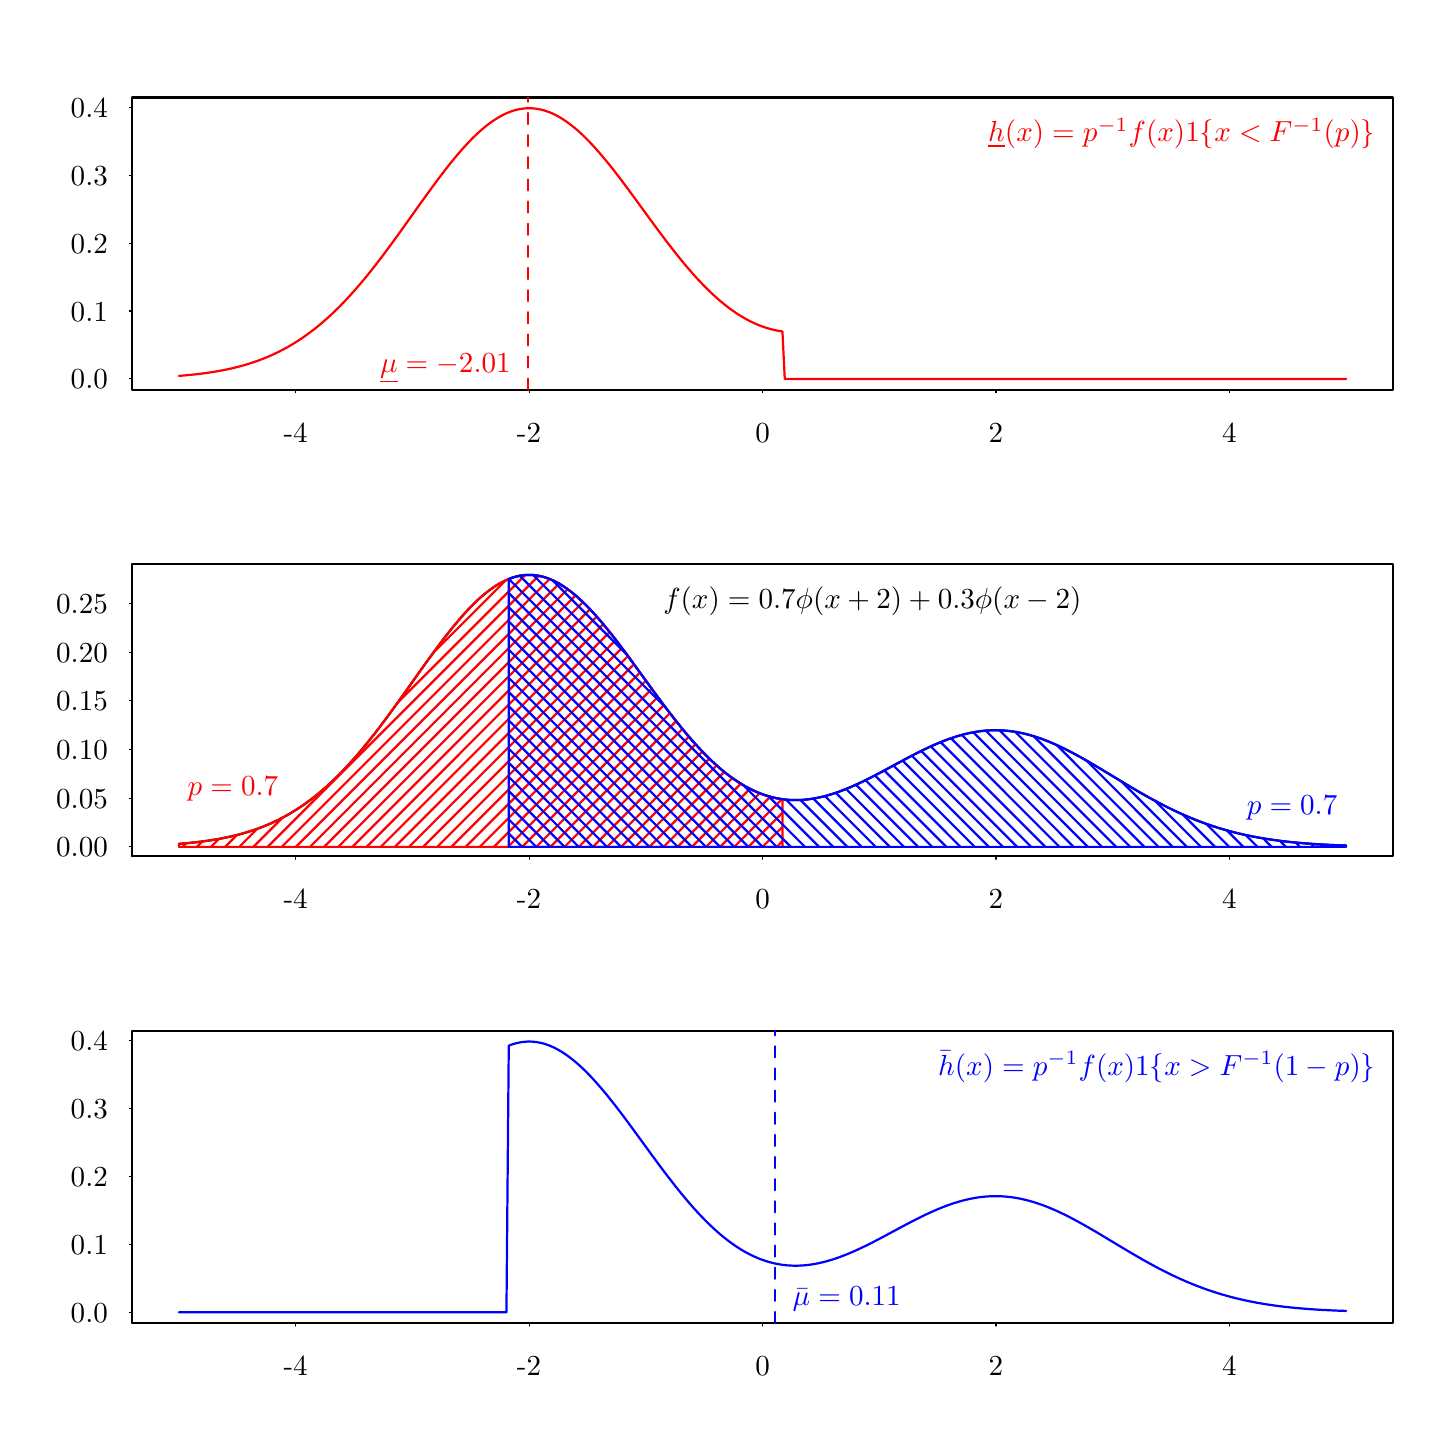
\begin{tikzpicture}[x=1pt,y=1pt]
\definecolor{fillColor}{RGB}{255,255,255}
\path[use as bounding box,fill=fillColor,fill opacity=0.00] (0,0) rectangle (505.89,505.89);
\begin{scope}
\path[clip] ( 37.80,375.06) rectangle (493.29,480.69);
\definecolor{drawColor}{RGB}{255,0,0}

\path[draw=drawColor,line width= 0.8pt,line join=round,line cap=round] ( 54.67,380.06) --
	( 55.52,380.13) --
	( 56.36,380.20) --
	( 57.21,380.27) --
	( 58.05,380.35) --
	( 58.90,380.43) --
	( 59.74,380.52) --
	( 60.59,380.61) --
	( 61.43,380.71) --
	( 62.28,380.81) --
	( 63.12,380.91) --
	( 63.97,381.03) --
	( 64.81,381.14) --
	( 65.66,381.27) --
	( 66.50,381.40) --
	( 67.35,381.53) --
	( 68.19,381.67) --
	( 69.04,381.82) --
	( 69.88,381.98) --
	( 70.73,382.14) --
	( 71.57,382.31) --
	( 72.42,382.49) --
	( 73.26,382.67) --
	( 74.11,382.87) --
	( 74.95,383.07) --
	( 75.80,383.28) --
	( 76.64,383.50) --
	( 77.49,383.73) --
	( 78.34,383.97) --
	( 79.18,384.22) --
	( 80.03,384.48) --
	( 80.87,384.75) --
	( 81.72,385.03) --
	( 82.56,385.32) --
	( 83.41,385.62) --
	( 84.25,385.94) --
	( 85.10,386.27) --
	( 85.94,386.60) --
	( 86.79,386.96) --
	( 87.63,387.32) --
	( 88.48,387.70) --
	( 89.32,388.09) --
	( 90.17,388.50) --
	( 91.01,388.91) --
	( 91.86,389.35) --
	( 92.70,389.79) --
	( 93.55,390.26) --
	( 94.39,390.73) --
	( 95.24,391.23) --
	( 96.08,391.74) --
	( 96.93,392.26) --
	( 97.77,392.80) --
	( 98.62,393.36) --
	( 99.47,393.93) --
	(100.31,394.52) --
	(101.16,395.12) --
	(102.00,395.75) --
	(102.85,396.39) --
	(103.69,397.04) --
	(104.54,397.72) --
	(105.38,398.41) --
	(106.23,399.12) --
	(107.07,399.84) --
	(107.92,400.59) --
	(108.76,401.35) --
	(109.61,402.13) --
	(110.45,402.93) --
	(111.30,403.74) --
	(112.14,404.57) --
	(112.99,405.42) --
	(113.83,406.28) --
	(114.68,407.17) --
	(115.52,408.07) --
	(116.37,408.98) --
	(117.21,409.92) --
	(118.06,410.86) --
	(118.90,411.83) --
	(119.75,412.81) --
	(120.59,413.80) --
	(121.44,414.82) --
	(122.29,415.84) --
	(123.13,416.88) --
	(123.98,417.93) --
	(124.82,419.00) --
	(125.67,420.08) --
	(126.51,421.17) --
	(127.36,422.27) --
	(128.20,423.38) --
	(129.05,424.50) --
	(129.89,425.64) --
	(130.74,426.78) --
	(131.58,427.93) --
	(132.43,429.09) --
	(133.27,430.25) --
	(134.12,431.42) --
	(134.96,432.60) --
	(135.81,433.78) --
	(136.65,434.96) --
	(137.50,436.15) --
	(138.34,437.34) --
	(139.19,438.52) --
	(140.03,439.71) --
	(140.88,440.90) --
	(141.72,442.09) --
	(142.57,443.27) --
	(143.41,444.45) --
	(144.26,445.62) --
	(145.11,446.78) --
	(145.95,447.94) --
	(146.80,449.09) --
	(147.64,450.24) --
	(148.49,451.37) --
	(149.33,452.49) --
	(150.18,453.59) --
	(151.02,454.68) --
	(151.87,455.76) --
	(152.71,456.82) --
	(153.56,457.87) --
	(154.40,458.90) --
	(155.25,459.90) --
	(156.09,460.89) --
	(156.94,461.86) --
	(157.78,462.80) --
	(158.63,463.72) --
	(159.47,464.62) --
	(160.32,465.49) --
	(161.16,466.34) --
	(162.01,467.15) --
	(162.85,467.94) --
	(163.70,468.71) --
	(164.54,469.44) --
	(165.39,470.14) --
	(166.24,470.81) --
	(167.08,471.44) --
	(167.93,472.05) --
	(168.77,472.62) --
	(169.62,473.15) --
	(170.46,473.65) --
	(171.31,474.12) --
	(172.15,474.55) --
	(173.00,474.94) --
	(173.84,475.30) --
	(174.69,475.62) --
	(175.53,475.90) --
	(176.38,476.14) --
	(177.22,476.34) --
	(178.07,476.51) --
	(178.91,476.63) --
	(179.76,476.72) --
	(180.60,476.77) --
	(181.45,476.78) --
	(182.29,476.75) --
	(183.14,476.68) --
	(183.98,476.57) --
	(184.83,476.42) --
	(185.67,476.24) --
	(186.52,476.01) --
	(187.36,475.75) --
	(188.21,475.45) --
	(189.06,475.11) --
	(189.90,474.74) --
	(190.75,474.32) --
	(191.59,473.88) --
	(192.44,473.39) --
	(193.28,472.87) --
	(194.13,472.32) --
	(194.97,471.73) --
	(195.82,471.11) --
	(196.66,470.46) --
	(197.51,469.78) --
	(198.35,469.06) --
	(199.20,468.32) --
	(200.04,467.55) --
	(200.89,466.75) --
	(201.73,465.92) --
	(202.58,465.06) --
	(203.42,464.18) --
	(204.27,463.28) --
	(205.11,462.35) --
	(205.96,461.40) --
	(206.80,460.43) --
	(207.65,459.44) --
	(208.49,458.43) --
	(209.34,457.41) --
	(210.19,456.36) --
	(211.03,455.30) --
	(211.88,454.23) --
	(212.72,453.14) --
	(213.57,452.04) --
	(214.41,450.93) --
	(215.26,449.81) --
	(216.10,448.68) --
	(216.95,447.54) --
	(217.79,446.40) --
	(218.64,445.24) --
	(219.48,444.09) --
	(220.33,442.93) --
	(221.17,441.77) --
	(222.02,440.61) --
	(222.86,439.45) --
	(223.71,438.29) --
	(224.55,437.13) --
	(225.40,435.97) --
	(226.24,434.82) --
	(227.09,433.67) --
	(227.93,432.53) --
	(228.78,431.40) --
	(229.62,430.27) --
	(230.47,429.15) --
	(231.31,428.04) --
	(232.16,426.94) --
	(233.01,425.86) --
	(233.85,424.78) --
	(234.70,423.72) --
	(235.54,422.67) --
	(236.39,421.63) --
	(237.23,420.61) --
	(238.08,419.60) --
	(238.92,418.61) --
	(239.77,417.64) --
	(240.61,416.68) --
	(241.46,415.74) --
	(242.30,414.82) --
	(243.15,413.92) --
	(243.99,413.04) --
	(244.84,412.18) --
	(245.68,411.33) --
	(246.53,410.51) --
	(247.37,409.71) --
	(248.22,408.93) --
	(249.06,408.17) --
	(249.91,407.43) --
	(250.75,406.71) --
	(251.60,406.02) --
	(252.44,405.35) --
	(253.29,404.70) --
	(254.13,404.07) --
	(254.98,403.47) --
	(255.83,402.89) --
	(256.67,402.33) --
	(257.52,401.80) --
	(258.36,401.29) --
	(259.21,400.80) --
	(260.05,400.33) --
	(260.90,399.89) --
	(261.74,399.48) --
	(262.59,399.08) --
	(263.43,398.71) --
	(264.28,398.36) --
	(265.12,398.03) --
	(265.97,397.73) --
	(266.81,397.45) --
	(267.66,397.19) --
	(268.50,396.96) --
	(269.35,396.74) --
	(270.19,396.55) --
	(271.04,396.38) --
	(271.88,396.24) --
	(272.73,396.11) --
	(273.57,378.97) --
	(274.42,378.97) --
	(275.26,378.97) --
	(276.11,378.97) --
	(276.96,378.97) --
	(277.80,378.97) --
	(278.65,378.97) --
	(279.49,378.97) --
	(280.34,378.97) --
	(281.18,378.97) --
	(282.03,378.97) --
	(282.87,378.97) --
	(283.72,378.97) --
	(284.56,378.97) --
	(285.41,378.97) --
	(286.25,378.97) --
	(287.10,378.97) --
	(287.94,378.97) --
	(288.79,378.97) --
	(289.63,378.97) --
	(290.48,378.97) --
	(291.32,378.97) --
	(292.17,378.97) --
	(293.01,378.97) --
	(293.86,378.97) --
	(294.70,378.97) --
	(295.55,378.97) --
	(296.39,378.97) --
	(297.24,378.97) --
	(298.08,378.97) --
	(298.93,378.97) --
	(299.78,378.97) --
	(300.62,378.97) --
	(301.47,378.97) --
	(302.31,378.97) --
	(303.16,378.97) --
	(304.00,378.97) --
	(304.85,378.97) --
	(305.69,378.97) --
	(306.54,378.97) --
	(307.38,378.97) --
	(308.23,378.97) --
	(309.07,378.97) --
	(309.92,378.97) --
	(310.76,378.97) --
	(311.61,378.97) --
	(312.45,378.97) --
	(313.30,378.97) --
	(314.14,378.97) --
	(314.99,378.97) --
	(315.83,378.97) --
	(316.68,378.97) --
	(317.52,378.97) --
	(318.37,378.97) --
	(319.21,378.97) --
	(320.06,378.97) --
	(320.90,378.97) --
	(321.75,378.97) --
	(322.60,378.97) --
	(323.44,378.97) --
	(324.29,378.97) --
	(325.13,378.97) --
	(325.98,378.97) --
	(326.82,378.97) --
	(327.67,378.97) --
	(328.51,378.97) --
	(329.36,378.97) --
	(330.20,378.97) --
	(331.05,378.97) --
	(331.89,378.97) --
	(332.74,378.97) --
	(333.58,378.97) --
	(334.43,378.97) --
	(335.27,378.97) --
	(336.12,378.97) --
	(336.96,378.97) --
	(337.81,378.97) --
	(338.65,378.97) --
	(339.50,378.97) --
	(340.34,378.97) --
	(341.19,378.97) --
	(342.03,378.97) --
	(342.88,378.97) --
	(343.73,378.97) --
	(344.57,378.97) --
	(345.42,378.97) --
	(346.26,378.97) --
	(347.11,378.97) --
	(347.95,378.97) --
	(348.80,378.97) --
	(349.64,378.97) --
	(350.49,378.97) --
	(351.33,378.97) --
	(352.18,378.97) --
	(353.02,378.97) --
	(353.87,378.97) --
	(354.71,378.97) --
	(355.56,378.97) --
	(356.40,378.97) --
	(357.25,378.97) --
	(358.09,378.97) --
	(358.94,378.97) --
	(359.78,378.97) --
	(360.63,378.97) --
	(361.47,378.97) --
	(362.32,378.97) --
	(363.16,378.97) --
	(364.01,378.97) --
	(364.85,378.97) --
	(365.70,378.97) --
	(366.55,378.97) --
	(367.39,378.97) --
	(368.24,378.97) --
	(369.08,378.97) --
	(369.93,378.97) --
	(370.77,378.97) --
	(371.62,378.97) --
	(372.46,378.97) --
	(373.31,378.97) --
	(374.15,378.97) --
	(375.00,378.97) --
	(375.84,378.97) --
	(376.69,378.97) --
	(377.53,378.97) --
	(378.38,378.97) --
	(379.22,378.97) --
	(380.07,378.97) --
	(380.91,378.97) --
	(381.76,378.97) --
	(382.60,378.97) --
	(383.45,378.97) --
	(384.29,378.97) --
	(385.14,378.97) --
	(385.98,378.97) --
	(386.83,378.97) --
	(387.68,378.97) --
	(388.52,378.97) --
	(389.37,378.97) --
	(390.21,378.97) --
	(391.06,378.97) --
	(391.90,378.97) --
	(392.75,378.97) --
	(393.59,378.97) --
	(394.44,378.97) --
	(395.28,378.97) --
	(396.13,378.97) --
	(396.97,378.97) --
	(397.82,378.97) --
	(398.66,378.97) --
	(399.51,378.97) --
	(400.35,378.97) --
	(401.20,378.97) --
	(402.04,378.97) --
	(402.89,378.97) --
	(403.73,378.97) --
	(404.58,378.97) --
	(405.42,378.97) --
	(406.27,378.97) --
	(407.11,378.97) --
	(407.96,378.97) --
	(408.80,378.97) --
	(409.65,378.97) --
	(410.50,378.97) --
	(411.34,378.97) --
	(412.19,378.97) --
	(413.03,378.97) --
	(413.88,378.97) --
	(414.72,378.97) --
	(415.57,378.97) --
	(416.41,378.97) --
	(417.26,378.97) --
	(418.10,378.97) --
	(418.95,378.97) --
	(419.79,378.97) --
	(420.64,378.97) --
	(421.48,378.97) --
	(422.33,378.97) --
	(423.17,378.97) --
	(424.02,378.97) --
	(424.86,378.97) --
	(425.71,378.97) --
	(426.55,378.97) --
	(427.40,378.97) --
	(428.24,378.97) --
	(429.09,378.97) --
	(429.93,378.97) --
	(430.78,378.97) --
	(431.62,378.97) --
	(432.47,378.97) --
	(433.32,378.97) --
	(434.16,378.97) --
	(435.01,378.97) --
	(435.85,378.97) --
	(436.70,378.97) --
	(437.54,378.97) --
	(438.39,378.97) --
	(439.23,378.97) --
	(440.08,378.97) --
	(440.92,378.97) --
	(441.77,378.97) --
	(442.61,378.97) --
	(443.46,378.97) --
	(444.30,378.97) --
	(445.15,378.97) --
	(445.99,378.97) --
	(446.84,378.97) --
	(447.68,378.97) --
	(448.53,378.97) --
	(449.37,378.97) --
	(450.22,378.97) --
	(451.06,378.97) --
	(451.91,378.97) --
	(452.75,378.97) --
	(453.60,378.97) --
	(454.45,378.97) --
	(455.29,378.97) --
	(456.14,378.97) --
	(456.98,378.97) --
	(457.83,378.97) --
	(458.67,378.97) --
	(459.52,378.97) --
	(460.36,378.97) --
	(461.21,378.97) --
	(462.05,378.97) --
	(462.90,378.97) --
	(463.74,378.97) --
	(464.59,378.97) --
	(465.43,378.97) --
	(466.28,378.97) --
	(467.12,378.97) --
	(467.97,378.97) --
	(468.81,378.97) --
	(469.66,378.97) --
	(470.50,378.97) --
	(471.35,378.97) --
	(472.19,378.97) --
	(473.04,378.97) --
	(473.88,378.97) --
	(474.73,378.97) --
	(475.57,378.97) --
	(476.42,378.97);
\end{scope}
\begin{scope}
\path[clip] (  0.00,  0.00) rectangle (505.89,505.89);
\definecolor{drawColor}{RGB}{0,0,0}

\path[draw=drawColor,line width= 0.4pt,line join=round,line cap=round] ( 96.84,375.06) -- (434.25,375.06);

\path[draw=drawColor,line width= 0.4pt,line join=round,line cap=round] ( 96.84,375.06) -- ( 96.84,374.00);

\path[draw=drawColor,line width= 0.4pt,line join=round,line cap=round] (181.19,375.06) -- (181.19,374.00);

\path[draw=drawColor,line width= 0.4pt,line join=round,line cap=round] (265.54,375.06) -- (265.54,374.00);

\path[draw=drawColor,line width= 0.4pt,line join=round,line cap=round] (349.89,375.06) -- (349.89,374.00);

\path[draw=drawColor,line width= 0.4pt,line join=round,line cap=round] (434.25,375.06) -- (434.25,374.00);

\node[text=drawColor,anchor=base,inner sep=0pt, outer sep=0pt, scale=  1.05] at ( 96.84,356.16) {-4};

\node[text=drawColor,anchor=base,inner sep=0pt, outer sep=0pt, scale=  1.05] at (181.19,356.16) {-2};

\node[text=drawColor,anchor=base,inner sep=0pt, outer sep=0pt, scale=  1.05] at (265.54,356.16) {0};

\node[text=drawColor,anchor=base,inner sep=0pt, outer sep=0pt, scale=  1.05] at (349.89,356.16) {2};

\node[text=drawColor,anchor=base,inner sep=0pt, outer sep=0pt, scale=  1.05] at (434.25,356.16) {4};

\path[draw=drawColor,line width= 0.4pt,line join=round,line cap=round] ( 37.80,378.97) -- ( 37.80,477.02);

\path[draw=drawColor,line width= 0.4pt,line join=round,line cap=round] ( 37.80,378.97) -- ( 36.74,378.97);

\path[draw=drawColor,line width= 0.4pt,line join=round,line cap=round] ( 37.80,403.49) -- ( 36.74,403.49);

\path[draw=drawColor,line width= 0.4pt,line join=round,line cap=round] ( 37.80,428.00) -- ( 36.74,428.00);

\path[draw=drawColor,line width= 0.4pt,line join=round,line cap=round] ( 37.80,452.51) -- ( 36.74,452.51);

\path[draw=drawColor,line width= 0.4pt,line join=round,line cap=round] ( 37.80,477.02) -- ( 36.74,477.02);

\node[text=drawColor,anchor=base east,inner sep=0pt, outer sep=0pt, scale=  1.05] at ( 28.98,375.36) {0.0};

\node[text=drawColor,anchor=base east,inner sep=0pt, outer sep=0pt, scale=  1.05] at ( 28.98,399.87) {0.1};

\node[text=drawColor,anchor=base east,inner sep=0pt, outer sep=0pt, scale=  1.05] at ( 28.98,424.38) {0.2};

\node[text=drawColor,anchor=base east,inner sep=0pt, outer sep=0pt, scale=  1.05] at ( 28.98,448.90) {0.3};

\node[text=drawColor,anchor=base east,inner sep=0pt, outer sep=0pt, scale=  1.05] at ( 28.98,473.41) {0.4};

\path[draw=drawColor,line width= 0.8pt,line join=round,line cap=round] ( 37.80,375.06) --
	(493.29,375.06) --
	(493.29,480.69) --
	( 37.80,480.69) --
	( 37.80,375.06);
\end{scope}
\begin{scope}
\path[clip] ( 37.80,375.06) rectangle (493.29,480.69);
\definecolor{drawColor}{RGB}{255,0,0}

\node[text=drawColor,anchor=base east,inner sep=0pt, outer sep=0pt, scale=  1.05] at (486.99,464.59) {$\underline{h}(x) = p^{-1}f(x) 1\{x < F^{-1}(p)\}$};

\path[draw=drawColor,line width= 0.8pt,dash pattern=on 4pt off 4pt ,line join=round,line cap=round] (180.82,375.06) -- (180.82,480.69);

\node[text=drawColor,anchor=base east,inner sep=0pt, outer sep=0pt, scale=  1.05] at (174.52,381.45) {$\underline{\mu} = -2.01$};
\end{scope}
\begin{scope}
\path[clip] ( 37.80,206.43) rectangle (493.29,312.06);
\definecolor{drawColor}{RGB}{0,0,0}

\path[draw=drawColor,line width= 0.8pt,line join=round,line cap=round] ( 54.67,210.97) --
	( 55.52,211.03) --
	( 56.36,211.10) --
	( 57.21,211.18) --
	( 58.05,211.26) --
	( 58.90,211.34) --
	( 59.74,211.43) --
	( 60.59,211.52) --
	( 61.43,211.62) --
	( 62.28,211.72) --
	( 63.12,211.83) --
	( 63.97,211.94) --
	( 64.81,212.06) --
	( 65.66,212.18) --
	( 66.50,212.31) --
	( 67.35,212.45) --
	( 68.19,212.59) --
	( 69.04,212.74) --
	( 69.88,212.89) --
	( 70.73,213.06) --
	( 71.57,213.23) --
	( 72.42,213.41) --
	( 73.26,213.59) --
	( 74.11,213.79) --
	( 74.95,213.99) --
	( 75.80,214.20) --
	( 76.64,214.42) --
	( 77.49,214.65) --
	( 78.34,214.90) --
	( 79.18,215.15) --
	( 80.03,215.41) --
	( 80.87,215.68) --
	( 81.72,215.96) --
	( 82.56,216.25) --
	( 83.41,216.56) --
	( 84.25,216.87) --
	( 85.10,217.20) --
	( 85.94,217.54) --
	( 86.79,217.90) --
	( 87.63,218.26) --
	( 88.48,218.64) --
	( 89.32,219.04) --
	( 90.17,219.44) --
	( 91.01,219.86) --
	( 91.86,220.30) --
	( 92.70,220.75) --
	( 93.55,221.21) --
	( 94.39,221.69) --
	( 95.24,222.19) --
	( 96.08,222.70) --
	( 96.93,223.23) --
	( 97.77,223.77) --
	( 98.62,224.33) --
	( 99.47,224.90) --
	(100.31,225.49) --
	(101.16,226.10) --
	(102.00,226.73) --
	(102.85,227.37) --
	(103.69,228.03) --
	(104.54,228.71) --
	(105.38,229.40) --
	(106.23,230.12) --
	(107.07,230.85) --
	(107.92,231.59) --
	(108.76,232.36) --
	(109.61,233.14) --
	(110.45,233.94) --
	(111.30,234.76) --
	(112.14,235.59) --
	(112.99,236.45) --
	(113.83,237.32) --
	(114.68,238.20) --
	(115.52,239.11) --
	(116.37,240.03) --
	(117.21,240.97) --
	(118.06,241.92) --
	(118.90,242.89) --
	(119.75,243.87) --
	(120.59,244.87) --
	(121.44,245.89) --
	(122.29,246.92) --
	(123.13,247.96) --
	(123.98,249.02) --
	(124.82,250.09) --
	(125.67,251.17) --
	(126.51,252.27) --
	(127.36,253.38) --
	(128.20,254.50) --
	(129.05,255.62) --
	(129.89,256.76) --
	(130.74,257.91) --
	(131.58,259.07) --
	(132.43,260.23) --
	(133.27,261.40) --
	(134.12,262.58) --
	(134.96,263.76) --
	(135.81,264.94) --
	(136.65,266.13) --
	(137.50,267.32) --
	(138.34,268.52) --
	(139.19,269.71) --
	(140.03,270.91) --
	(140.88,272.10) --
	(141.72,273.29) --
	(142.57,274.48) --
	(143.41,275.66) --
	(144.26,276.84) --
	(145.11,278.01) --
	(145.95,279.18) --
	(146.80,280.33) --
	(147.64,281.48) --
	(148.49,282.61) --
	(149.33,283.74) --
	(150.18,284.85) --
	(151.02,285.95) --
	(151.87,287.03) --
	(152.71,288.10) --
	(153.56,289.15) --
	(154.40,290.18) --
	(155.25,291.19) --
	(156.09,292.19) --
	(156.94,293.16) --
	(157.78,294.11) --
	(158.63,295.03) --
	(159.47,295.93) --
	(160.32,296.81) --
	(161.16,297.66) --
	(162.01,298.48) --
	(162.85,299.27) --
	(163.70,300.04) --
	(164.54,300.77) --
	(165.39,301.47) --
	(166.24,302.15) --
	(167.08,302.79) --
	(167.93,303.39) --
	(168.77,303.97) --
	(169.62,304.51) --
	(170.46,305.01) --
	(171.31,305.48) --
	(172.15,305.91) --
	(173.00,306.30) --
	(173.84,306.66) --
	(174.69,306.98) --
	(175.53,307.26) --
	(176.38,307.50) --
	(177.22,307.71) --
	(178.07,307.88) --
	(178.91,308.00) --
	(179.76,308.09) --
	(180.60,308.14) --
	(181.45,308.15) --
	(182.29,308.12) --
	(183.14,308.05) --
	(183.98,307.94) --
	(184.83,307.79) --
	(185.67,307.60) --
	(186.52,307.38) --
	(187.36,307.11) --
	(188.21,306.81) --
	(189.06,306.47) --
	(189.90,306.10) --
	(190.75,305.68) --
	(191.59,305.23) --
	(192.44,304.75) --
	(193.28,304.22) --
	(194.13,303.67) --
	(194.97,303.08) --
	(195.82,302.46) --
	(196.66,301.80) --
	(197.51,301.12) --
	(198.35,300.40) --
	(199.20,299.65) --
	(200.04,298.87) --
	(200.89,298.07) --
	(201.73,297.24) --
	(202.58,296.38) --
	(203.42,295.49) --
	(204.27,294.59) --
	(205.11,293.65) --
	(205.96,292.70) --
	(206.80,291.73) --
	(207.65,290.73) --
	(208.49,289.72) --
	(209.34,288.68) --
	(210.19,287.63) --
	(211.03,286.57) --
	(211.88,285.49) --
	(212.72,284.40) --
	(213.57,283.29) --
	(214.41,282.18) --
	(215.26,281.05) --
	(216.10,279.91) --
	(216.95,278.77) --
	(217.79,277.62) --
	(218.64,276.46) --
	(219.48,275.30) --
	(220.33,274.14) --
	(221.17,272.97) --
	(222.02,271.81) --
	(222.86,270.64) --
	(223.71,269.47) --
	(224.55,268.31) --
	(225.40,267.15) --
	(226.24,265.99) --
	(227.09,264.84) --
	(227.93,263.69) --
	(228.78,262.55) --
	(229.62,261.42) --
	(230.47,260.29) --
	(231.31,259.18) --
	(232.16,258.08) --
	(233.01,256.98) --
	(233.85,255.90) --
	(234.70,254.83) --
	(235.54,253.78) --
	(236.39,252.74) --
	(237.23,251.71) --
	(238.08,250.70) --
	(238.92,249.71) --
	(239.77,248.73) --
	(240.61,247.77) --
	(241.46,246.82) --
	(242.30,245.90) --
	(243.15,244.99) --
	(243.99,244.10) --
	(244.84,243.24) --
	(245.68,242.39) --
	(246.53,241.56) --
	(247.37,240.76) --
	(248.22,239.97) --
	(249.06,239.21) --
	(249.91,238.47) --
	(250.75,237.75) --
	(251.60,237.05) --
	(252.44,236.38) --
	(253.29,235.73) --
	(254.13,235.10) --
	(254.98,234.49) --
	(255.83,233.91) --
	(256.67,233.35) --
	(257.52,232.81) --
	(258.36,232.30) --
	(259.21,231.81) --
	(260.05,231.34) --
	(260.90,230.90) --
	(261.74,230.48) --
	(262.59,230.08) --
	(263.43,229.70) --
	(264.28,229.35) --
	(265.12,229.03) --
	(265.97,228.72) --
	(266.81,228.44) --
	(267.66,228.18) --
	(268.50,227.94) --
	(269.35,227.73) --
	(270.19,227.54) --
	(271.04,227.37) --
	(271.88,227.22) --
	(272.73,227.09) --
	(273.57,226.99) --
	(274.42,226.90) --
	(275.26,226.84) --
	(276.11,226.80) --
	(276.96,226.78) --
	(277.80,226.77) --
	(278.65,226.79) --
	(279.49,226.83) --
	(280.34,226.88) --
	(281.18,226.96) --
	(282.03,227.05) --
	(282.87,227.16) --
	(283.72,227.29) --
	(284.56,227.44) --
	(285.41,227.60) --
	(286.25,227.78) --
	(287.10,227.97) --
	(287.94,228.18) --
	(288.79,228.41) --
	(289.63,228.65) --
	(290.48,228.91) --
	(291.32,229.18) --
	(292.17,229.46) --
	(293.01,229.76) --
	(293.86,230.07) --
	(294.70,230.39) --
	(295.55,230.72) --
	(296.39,231.07) --
	(297.24,231.42) --
	(298.08,231.79) --
	(298.93,232.16) --
	(299.78,232.55) --
	(300.62,232.94) --
	(301.47,233.34) --
	(302.31,233.75) --
	(303.16,234.16) --
	(304.00,234.59) --
	(304.85,235.01) --
	(305.69,235.45) --
	(306.54,235.89) --
	(307.38,236.33) --
	(308.23,236.78) --
	(309.07,237.23) --
	(309.92,237.68) --
	(310.76,238.13) --
	(311.61,238.59) --
	(312.45,239.05) --
	(313.30,239.50) --
	(314.14,239.96) --
	(314.99,240.41) --
	(315.83,240.87) --
	(316.68,241.32) --
	(317.52,241.77) --
	(318.37,242.22) --
	(319.21,242.66) --
	(320.06,243.10) --
	(320.90,243.53) --
	(321.75,243.96) --
	(322.60,244.38) --
	(323.44,244.80) --
	(324.29,245.21) --
	(325.13,245.61) --
	(325.98,246.00) --
	(326.82,246.39) --
	(327.67,246.76) --
	(328.51,247.13) --
	(329.36,247.48) --
	(330.20,247.83) --
	(331.05,248.16) --
	(331.89,248.49) --
	(332.74,248.80) --
	(333.58,249.09) --
	(334.43,249.38) --
	(335.27,249.65) --
	(336.12,249.91) --
	(336.96,250.16) --
	(337.81,250.39) --
	(338.65,250.61) --
	(339.50,250.81) --
	(340.34,251.00) --
	(341.19,251.17) --
	(342.03,251.33) --
	(342.88,251.47) --
	(343.73,251.60) --
	(344.57,251.71) --
	(345.42,251.80) --
	(346.26,251.88) --
	(347.11,251.94) --
	(347.95,251.98) --
	(348.80,252.01) --
	(349.64,252.02) --
	(350.49,252.01) --
	(351.33,251.99) --
	(352.18,251.95) --
	(353.02,251.89) --
	(353.87,251.82) --
	(354.71,251.73) --
	(355.56,251.63) --
	(356.40,251.51) --
	(357.25,251.37) --
	(358.09,251.21) --
	(358.94,251.04) --
	(359.78,250.86) --
	(360.63,250.66) --
	(361.47,250.44) --
	(362.32,250.21) --
	(363.16,249.96) --
	(364.01,249.70) --
	(364.85,249.43) --
	(365.70,249.14) --
	(366.55,248.84) --
	(367.39,248.52) --
	(368.24,248.19) --
	(369.08,247.85) --
	(369.93,247.50) --
	(370.77,247.13) --
	(371.62,246.76) --
	(372.46,246.37) --
	(373.31,245.98) --
	(374.15,245.57) --
	(375.00,245.15) --
	(375.84,244.73) --
	(376.69,244.29) --
	(377.53,243.85) --
	(378.38,243.40) --
	(379.22,242.94) --
	(380.07,242.48) --
	(380.91,242.01) --
	(381.76,241.53) --
	(382.60,241.05) --
	(383.45,240.56) --
	(384.29,240.07) --
	(385.14,239.58) --
	(385.98,239.08) --
	(386.83,238.57) --
	(387.68,238.07) --
	(388.52,237.56) --
	(389.37,237.05) --
	(390.21,236.54) --
	(391.06,236.03) --
	(391.90,235.52) --
	(392.75,235.01) --
	(393.59,234.50) --
	(394.44,233.98) --
	(395.28,233.48) --
	(396.13,232.97) --
	(396.97,232.46) --
	(397.82,231.96) --
	(398.66,231.46) --
	(399.51,230.96) --
	(400.35,230.46) --
	(401.20,229.97) --
	(402.04,229.48) --
	(402.89,229.00) --
	(403.73,228.52) --
	(404.58,228.04) --
	(405.42,227.57) --
	(406.27,227.11) --
	(407.11,226.65) --
	(407.96,226.20) --
	(408.80,225.75) --
	(409.65,225.31) --
	(410.50,224.87) --
	(411.34,224.45) --
	(412.19,224.02) --
	(413.03,223.61) --
	(413.88,223.20) --
	(414.72,222.80) --
	(415.57,222.40) --
	(416.41,222.02) --
	(417.26,221.64) --
	(418.10,221.26) --
	(418.95,220.90) --
	(419.79,220.54) --
	(420.64,220.19) --
	(421.48,219.85) --
	(422.33,219.51) --
	(423.17,219.18) --
	(424.02,218.86) --
	(424.86,218.55) --
	(425.71,218.24) --
	(426.55,217.95) --
	(427.40,217.66) --
	(428.24,217.37) --
	(429.09,217.10) --
	(429.93,216.83) --
	(430.78,216.57) --
	(431.62,216.32) --
	(432.47,216.07) --
	(433.32,215.83) --
	(434.16,215.60) --
	(435.01,215.37) --
	(435.85,215.15) --
	(436.70,214.94) --
	(437.54,214.73) --
	(438.39,214.53) --
	(439.23,214.34) --
	(440.08,214.16) --
	(440.92,213.98) --
	(441.77,213.80) --
	(442.61,213.63) --
	(443.46,213.47) --
	(444.30,213.31) --
	(445.15,213.16) --
	(445.99,213.02) --
	(446.84,212.87) --
	(447.68,212.74) --
	(448.53,212.61) --
	(449.37,212.48) --
	(450.22,212.36) --
	(451.06,212.25) --
	(451.91,212.13) --
	(452.75,212.03) --
	(453.60,211.92) --
	(454.45,211.82) --
	(455.29,211.73) --
	(456.14,211.64) --
	(456.98,211.55) --
	(457.83,211.47) --
	(458.67,211.39) --
	(459.52,211.31) --
	(460.36,211.24) --
	(461.21,211.17) --
	(462.05,211.10) --
	(462.90,211.04) --
	(463.74,210.98) --
	(464.59,210.92) --
	(465.43,210.86) --
	(466.28,210.81) --
	(467.12,210.76) --
	(467.97,210.71) --
	(468.81,210.67) --
	(469.66,210.62) --
	(470.50,210.58) --
	(471.35,210.54) --
	(472.19,210.50) --
	(473.04,210.47) --
	(473.88,210.43) --
	(474.73,210.40) --
	(475.57,210.37) --
	(476.42,210.34);
\end{scope}
\begin{scope}
\path[clip] (  0.00,  0.00) rectangle (505.89,505.89);
\definecolor{drawColor}{RGB}{0,0,0}

\path[draw=drawColor,line width= 0.4pt,line join=round,line cap=round] ( 96.84,206.43) -- (434.25,206.43);

\path[draw=drawColor,line width= 0.4pt,line join=round,line cap=round] ( 96.84,206.43) -- ( 96.84,205.37);

\path[draw=drawColor,line width= 0.4pt,line join=round,line cap=round] (181.19,206.43) -- (181.19,205.37);

\path[draw=drawColor,line width= 0.4pt,line join=round,line cap=round] (265.54,206.43) -- (265.54,205.37);

\path[draw=drawColor,line width= 0.4pt,line join=round,line cap=round] (349.89,206.43) -- (349.89,205.37);

\path[draw=drawColor,line width= 0.4pt,line join=round,line cap=round] (434.25,206.43) -- (434.25,205.37);

\node[text=drawColor,anchor=base,inner sep=0pt, outer sep=0pt, scale=  1.05] at ( 96.84,187.53) {-4};

\node[text=drawColor,anchor=base,inner sep=0pt, outer sep=0pt, scale=  1.05] at (181.19,187.53) {-2};

\node[text=drawColor,anchor=base,inner sep=0pt, outer sep=0pt, scale=  1.05] at (265.54,187.53) {0};

\node[text=drawColor,anchor=base,inner sep=0pt, outer sep=0pt, scale=  1.05] at (349.89,187.53) {2};

\node[text=drawColor,anchor=base,inner sep=0pt, outer sep=0pt, scale=  1.05] at (434.25,187.53) {4};

\path[draw=drawColor,line width= 0.4pt,line join=round,line cap=round] ( 37.80,209.87) -- ( 37.80,297.84);

\path[draw=drawColor,line width= 0.4pt,line join=round,line cap=round] ( 37.80,209.87) -- ( 36.74,209.87);

\path[draw=drawColor,line width= 0.4pt,line join=round,line cap=round] ( 37.80,227.47) -- ( 36.74,227.47);

\path[draw=drawColor,line width= 0.4pt,line join=round,line cap=round] ( 37.80,245.06) -- ( 36.74,245.06);

\path[draw=drawColor,line width= 0.4pt,line join=round,line cap=round] ( 37.80,262.65) -- ( 36.74,262.65);

\path[draw=drawColor,line width= 0.4pt,line join=round,line cap=round] ( 37.80,280.25) -- ( 36.74,280.25);

\path[draw=drawColor,line width= 0.4pt,line join=round,line cap=round] ( 37.80,297.84) -- ( 36.74,297.84);

\node[text=drawColor,anchor=base east,inner sep=0pt, outer sep=0pt, scale=  1.05] at ( 28.98,206.26) {0.00};

\node[text=drawColor,anchor=base east,inner sep=0pt, outer sep=0pt, scale=  1.05] at ( 28.98,223.85) {0.05};

\node[text=drawColor,anchor=base east,inner sep=0pt, outer sep=0pt, scale=  1.05] at ( 28.98,241.44) {0.10};

\node[text=drawColor,anchor=base east,inner sep=0pt, outer sep=0pt, scale=  1.05] at ( 28.98,259.04) {0.15};

\node[text=drawColor,anchor=base east,inner sep=0pt, outer sep=0pt, scale=  1.05] at ( 28.98,276.63) {0.20};

\node[text=drawColor,anchor=base east,inner sep=0pt, outer sep=0pt, scale=  1.05] at ( 28.98,294.22) {0.25};

\path[draw=drawColor,line width= 0.8pt,line join=round,line cap=round] ( 37.80,206.43) --
	(493.29,206.43) --
	(493.29,312.06) --
	( 37.80,312.06) --
	( 37.80,206.43);
\end{scope}
\begin{scope}
\path[clip] ( 37.80,206.43) rectangle (493.29,312.06);
\definecolor{drawColor}{RGB}{255,0,0}

\path[draw=drawColor,line width= 0.8pt,line join=round,line cap=round] ( 56.02,209.87) -- ( 57.34,211.19);

\path[draw=drawColor,line width= 0.8pt,line join=round,line cap=round] ( 61.13,209.87) -- ( 63.08,211.82);

\path[draw=drawColor,line width= 0.8pt,line join=round,line cap=round] ( 66.24,209.87) -- ( 69.12,212.75);

\path[draw=drawColor,line width= 0.8pt,line join=round,line cap=round] ( 71.36,209.87) -- ( 75.64,214.16);

\path[draw=drawColor,line width= 0.8pt,line join=round,line cap=round] ( 76.47,209.87) -- ( 83.00,216.41);

\path[draw=drawColor,line width= 0.8pt,line join=round,line cap=round] (146.45,279.86) -- (172.80,306.21);

\path[draw=drawColor,line width= 0.8pt,line join=round,line cap=round] ( 81.58,209.87) -- ( 92.16,220.46);

\path[draw=drawColor,line width= 0.8pt,line join=round,line cap=round] (133.71,262.01) -- (179.79,308.09);

\path[draw=drawColor,line width= 0.8pt,line join=round,line cap=round] ( 86.69,209.87) -- (184.64,307.82);

\path[draw=drawColor,line width= 0.8pt,line join=round,line cap=round] ( 91.80,209.87) -- (188.58,306.66);

\path[draw=drawColor,line width= 0.8pt,line join=round,line cap=round] ( 96.91,209.87) -- (192.02,304.99);

\path[draw=drawColor,line width= 0.8pt,line join=round,line cap=round] (102.02,209.87) -- (195.12,302.97);

\path[draw=drawColor,line width= 0.8pt,line join=round,line cap=round] (107.13,209.87) -- (197.97,300.72);

\path[draw=drawColor,line width= 0.8pt,line join=round,line cap=round] (112.24,209.87) -- (200.65,298.29);

\path[draw=drawColor,line width= 0.8pt,line join=round,line cap=round] (117.35,209.87) -- (203.20,295.73);

\path[draw=drawColor,line width= 0.8pt,line join=round,line cap=round] (122.46,209.87) -- (205.64,293.06);

\path[draw=drawColor,line width= 0.8pt,line join=round,line cap=round] (127.57,209.87) -- (208.00,290.31);

\path[draw=drawColor,line width= 0.8pt,line join=round,line cap=round] (132.68,209.87) -- (210.30,287.49);

\path[draw=drawColor,line width= 0.8pt,line join=round,line cap=round] (137.79,209.87) -- (212.54,284.63);

\path[draw=drawColor,line width= 0.8pt,line join=round,line cap=round] (142.90,209.87) -- (214.75,281.72);

\path[draw=drawColor,line width= 0.8pt,line join=round,line cap=round] (148.01,209.87) -- (216.93,278.79);

\path[draw=drawColor,line width= 0.8pt,line join=round,line cap=round] (153.12,209.87) -- (219.09,275.84);

\path[draw=drawColor,line width= 0.8pt,line join=round,line cap=round] (158.23,209.87) -- (221.24,272.88);

\path[draw=drawColor,line width= 0.8pt,line join=round,line cap=round] (163.34,209.87) -- (223.39,269.92);

\path[draw=drawColor,line width= 0.8pt,line join=round,line cap=round] (168.45,209.87) -- (225.54,266.96);

\path[draw=drawColor,line width= 0.8pt,line join=round,line cap=round] (173.56,209.87) -- (227.70,264.01);

\path[draw=drawColor,line width= 0.8pt,line join=round,line cap=round] (178.67,209.87) -- (229.88,261.08);

\path[draw=drawColor,line width= 0.8pt,line join=round,line cap=round] (183.78,209.87) -- (232.08,258.18);

\path[draw=drawColor,line width= 0.8pt,line join=round,line cap=round] (188.89,209.87) -- (234.32,255.31);

\path[draw=drawColor,line width= 0.8pt,line join=round,line cap=round] (194.00,209.87) -- (236.60,252.47);

\path[draw=drawColor,line width= 0.8pt,line join=round,line cap=round] (199.11,209.87) -- (238.93,249.69);

\path[draw=drawColor,line width= 0.8pt,line join=round,line cap=round] (204.22,209.87) -- (241.32,246.97);

\path[draw=drawColor,line width= 0.8pt,line join=round,line cap=round] (209.33,209.87) -- (243.78,244.32);

\path[draw=drawColor,line width= 0.8pt,line join=round,line cap=round] (214.44,209.87) -- (246.33,241.76);

\path[draw=drawColor,line width= 0.8pt,line join=round,line cap=round] (219.55,209.87) -- (248.97,239.29);

\path[draw=drawColor,line width= 0.8pt,line join=round,line cap=round] (224.66,209.87) -- (251.73,236.95);

\path[draw=drawColor,line width= 0.8pt,line join=round,line cap=round] (229.77,209.87) -- (254.64,234.74);

\path[draw=drawColor,line width= 0.8pt,line join=round,line cap=round] (234.88,209.87) -- (257.70,232.70);

\path[draw=drawColor,line width= 0.8pt,line join=round,line cap=round] (239.99,209.87) -- (260.98,230.86);

\path[draw=drawColor,line width= 0.8pt,line join=round,line cap=round] (245.10,209.87) -- (264.50,229.27);

\path[draw=drawColor,line width= 0.8pt,line join=round,line cap=round] (250.21,209.87) -- (268.33,227.99);

\path[draw=drawColor,line width= 0.8pt,line join=round,line cap=round] (255.32,209.87) -- (272.57,227.12);

\path[draw=drawColor,line width= 0.8pt,line join=round,line cap=round] (260.43,209.87) -- (272.73,222.17);

\path[draw=drawColor,line width= 0.8pt,line join=round,line cap=round] (265.54,209.87) -- (272.73,217.06);

\path[draw=drawColor,line width= 0.8pt,line join=round,line cap=round] (270.66,209.87) -- (272.73,211.95);

\path[draw=drawColor,line width= 0.8pt,line join=round,line cap=round] ( 54.67,209.87) --
	( 55.52,209.87) --
	( 56.36,209.87) --
	( 57.21,209.87) --
	( 58.05,209.87) --
	( 58.90,209.87) --
	( 59.74,209.87) --
	( 60.59,209.87) --
	( 61.43,209.87) --
	( 62.28,209.87) --
	( 63.12,209.87) --
	( 63.97,209.87) --
	( 64.81,209.87) --
	( 65.66,209.87) --
	( 66.50,209.87) --
	( 67.35,209.87) --
	( 68.19,209.87) --
	( 69.04,209.87) --
	( 69.88,209.87) --
	( 70.73,209.87) --
	( 71.57,209.87) --
	( 72.42,209.87) --
	( 73.26,209.87) --
	( 74.11,209.87) --
	( 74.95,209.87) --
	( 75.80,209.87) --
	( 76.64,209.87) --
	( 77.49,209.87) --
	( 78.34,209.87) --
	( 79.18,209.87) --
	( 80.03,209.87) --
	( 80.87,209.87) --
	( 81.72,209.87) --
	( 82.56,209.87) --
	( 83.41,209.87) --
	( 84.25,209.87) --
	( 85.10,209.87) --
	( 85.94,209.87) --
	( 86.79,209.87) --
	( 87.63,209.87) --
	( 88.48,209.87) --
	( 89.32,209.87) --
	( 90.17,209.87) --
	( 91.01,209.87) --
	( 91.86,209.87) --
	( 92.70,209.87) --
	( 93.55,209.87) --
	( 94.39,209.87) --
	( 95.24,209.87) --
	( 96.08,209.87) --
	( 96.93,209.87) --
	( 97.77,209.87) --
	( 98.62,209.87) --
	( 99.47,209.87) --
	(100.31,209.87) --
	(101.16,209.87) --
	(102.00,209.87) --
	(102.85,209.87) --
	(103.69,209.87) --
	(104.54,209.87) --
	(105.38,209.87) --
	(106.23,209.87) --
	(107.07,209.87) --
	(107.92,209.87) --
	(108.76,209.87) --
	(109.61,209.87) --
	(110.45,209.87) --
	(111.30,209.87) --
	(112.14,209.87) --
	(112.99,209.87) --
	(113.83,209.87) --
	(114.68,209.87) --
	(115.52,209.87) --
	(116.37,209.87) --
	(117.21,209.87) --
	(118.06,209.87) --
	(118.90,209.87) --
	(119.75,209.87) --
	(120.59,209.87) --
	(121.44,209.87) --
	(122.29,209.87) --
	(123.13,209.87) --
	(123.98,209.87) --
	(124.82,209.87) --
	(125.67,209.87) --
	(126.51,209.87) --
	(127.36,209.87) --
	(128.20,209.87) --
	(129.05,209.87) --
	(129.89,209.87) --
	(130.74,209.87) --
	(131.58,209.87) --
	(132.43,209.87) --
	(133.27,209.87) --
	(134.12,209.87) --
	(134.96,209.87) --
	(135.81,209.87) --
	(136.65,209.87) --
	(137.50,209.87) --
	(138.34,209.87) --
	(139.19,209.87) --
	(140.03,209.87) --
	(140.88,209.87) --
	(141.72,209.87) --
	(142.57,209.87) --
	(143.41,209.87) --
	(144.26,209.87) --
	(145.11,209.87) --
	(145.95,209.87) --
	(146.80,209.87) --
	(147.64,209.87) --
	(148.49,209.87) --
	(149.33,209.87) --
	(150.18,209.87) --
	(151.02,209.87) --
	(151.87,209.87) --
	(152.71,209.87) --
	(153.56,209.87) --
	(154.40,209.87) --
	(155.25,209.87) --
	(156.09,209.87) --
	(156.94,209.87) --
	(157.78,209.87) --
	(158.63,209.87) --
	(159.47,209.87) --
	(160.32,209.87) --
	(161.16,209.87) --
	(162.01,209.87) --
	(162.85,209.87) --
	(163.70,209.87) --
	(164.54,209.87) --
	(165.39,209.87) --
	(166.24,209.87) --
	(167.08,209.87) --
	(167.93,209.87) --
	(168.77,209.87) --
	(169.62,209.87) --
	(170.46,209.87) --
	(171.31,209.87) --
	(172.15,209.87) --
	(173.00,209.87) --
	(173.84,209.87) --
	(174.69,209.87) --
	(175.53,209.87) --
	(176.38,209.87) --
	(177.22,209.87) --
	(178.07,209.87) --
	(178.91,209.87) --
	(179.76,209.87) --
	(180.60,209.87) --
	(181.45,209.87) --
	(182.29,209.87) --
	(183.14,209.87) --
	(183.98,209.87) --
	(184.83,209.87) --
	(185.67,209.87) --
	(186.52,209.87) --
	(187.36,209.87) --
	(188.21,209.87) --
	(189.06,209.87) --
	(189.90,209.87) --
	(190.75,209.87) --
	(191.59,209.87) --
	(192.44,209.87) --
	(193.28,209.87) --
	(194.13,209.87) --
	(194.97,209.87) --
	(195.82,209.87) --
	(196.66,209.87) --
	(197.51,209.87) --
	(198.35,209.87) --
	(199.20,209.87) --
	(200.04,209.87) --
	(200.89,209.87) --
	(201.73,209.87) --
	(202.58,209.87) --
	(203.42,209.87) --
	(204.27,209.87) --
	(205.11,209.87) --
	(205.96,209.87) --
	(206.80,209.87) --
	(207.65,209.87) --
	(208.49,209.87) --
	(209.34,209.87) --
	(210.19,209.87) --
	(211.03,209.87) --
	(211.88,209.87) --
	(212.72,209.87) --
	(213.57,209.87) --
	(214.41,209.87) --
	(215.26,209.87) --
	(216.10,209.87) --
	(216.95,209.87) --
	(217.79,209.87) --
	(218.64,209.87) --
	(219.48,209.87) --
	(220.33,209.87) --
	(221.17,209.87) --
	(222.02,209.87) --
	(222.86,209.87) --
	(223.71,209.87) --
	(224.55,209.87) --
	(225.40,209.87) --
	(226.24,209.87) --
	(227.09,209.87) --
	(227.93,209.87) --
	(228.78,209.87) --
	(229.62,209.87) --
	(230.47,209.87) --
	(231.31,209.87) --
	(232.16,209.87) --
	(233.01,209.87) --
	(233.85,209.87) --
	(234.70,209.87) --
	(235.54,209.87) --
	(236.39,209.87) --
	(237.23,209.87) --
	(238.08,209.87) --
	(238.92,209.87) --
	(239.77,209.87) --
	(240.61,209.87) --
	(241.46,209.87) --
	(242.30,209.87) --
	(243.15,209.87) --
	(243.99,209.87) --
	(244.84,209.87) --
	(245.68,209.87) --
	(246.53,209.87) --
	(247.37,209.87) --
	(248.22,209.87) --
	(249.06,209.87) --
	(249.91,209.87) --
	(250.75,209.87) --
	(251.60,209.87) --
	(252.44,209.87) --
	(253.29,209.87) --
	(254.13,209.87) --
	(254.98,209.87) --
	(255.83,209.87) --
	(256.67,209.87) --
	(257.52,209.87) --
	(258.36,209.87) --
	(259.21,209.87) --
	(260.05,209.87) --
	(260.90,209.87) --
	(261.74,209.87) --
	(262.59,209.87) --
	(263.43,209.87) --
	(264.28,209.87) --
	(265.12,209.87) --
	(265.97,209.87) --
	(266.81,209.87) --
	(267.66,209.87) --
	(268.50,209.87) --
	(269.35,209.87) --
	(270.19,209.87) --
	(271.04,209.87) --
	(271.88,209.87) --
	(272.73,209.87) --
	(272.73,227.09) --
	(271.88,227.22) --
	(271.04,227.37) --
	(270.19,227.54) --
	(269.35,227.73) --
	(268.50,227.94) --
	(267.66,228.18) --
	(266.81,228.44) --
	(265.97,228.72) --
	(265.12,229.03) --
	(264.28,229.35) --
	(263.43,229.70) --
	(262.59,230.08) --
	(261.74,230.48) --
	(260.90,230.90) --
	(260.05,231.34) --
	(259.21,231.81) --
	(258.36,232.30) --
	(257.52,232.81) --
	(256.67,233.35) --
	(255.83,233.91) --
	(254.98,234.49) --
	(254.13,235.10) --
	(253.29,235.73) --
	(252.44,236.38) --
	(251.60,237.05) --
	(250.75,237.75) --
	(249.91,238.47) --
	(249.06,239.21) --
	(248.22,239.97) --
	(247.37,240.76) --
	(246.53,241.56) --
	(245.68,242.39) --
	(244.84,243.24) --
	(243.99,244.10) --
	(243.15,244.99) --
	(242.30,245.90) --
	(241.46,246.82) --
	(240.61,247.77) --
	(239.77,248.73) --
	(238.92,249.71) --
	(238.08,250.70) --
	(237.23,251.71) --
	(236.39,252.74) --
	(235.54,253.78) --
	(234.70,254.83) --
	(233.85,255.90) --
	(233.01,256.98) --
	(232.16,258.08) --
	(231.31,259.18) --
	(230.47,260.29) --
	(229.62,261.42) --
	(228.78,262.55) --
	(227.93,263.69) --
	(227.09,264.84) --
	(226.24,265.99) --
	(225.40,267.15) --
	(224.55,268.31) --
	(223.71,269.47) --
	(222.86,270.64) --
	(222.02,271.81) --
	(221.17,272.97) --
	(220.33,274.14) --
	(219.48,275.30) --
	(218.64,276.46) --
	(217.79,277.62) --
	(216.95,278.77) --
	(216.10,279.91) --
	(215.26,281.05) --
	(214.41,282.18) --
	(213.57,283.29) --
	(212.72,284.40) --
	(211.88,285.49) --
	(211.03,286.57) --
	(210.19,287.63) --
	(209.34,288.68) --
	(208.49,289.72) --
	(207.65,290.73) --
	(206.80,291.73) --
	(205.96,292.70) --
	(205.11,293.65) --
	(204.27,294.59) --
	(203.42,295.49) --
	(202.58,296.38) --
	(201.73,297.24) --
	(200.89,298.07) --
	(200.04,298.87) --
	(199.20,299.65) --
	(198.35,300.40) --
	(197.51,301.12) --
	(196.66,301.80) --
	(195.82,302.46) --
	(194.97,303.08) --
	(194.13,303.67) --
	(193.28,304.22) --
	(192.44,304.75) --
	(191.59,305.23) --
	(190.75,305.68) --
	(189.90,306.10) --
	(189.06,306.47) --
	(188.21,306.81) --
	(187.36,307.11) --
	(186.52,307.38) --
	(185.67,307.60) --
	(184.83,307.79) --
	(183.98,307.94) --
	(183.14,308.05) --
	(182.29,308.12) --
	(181.45,308.15) --
	(180.60,308.14) --
	(179.76,308.09) --
	(178.91,308.00) --
	(178.07,307.88) --
	(177.22,307.71) --
	(176.38,307.50) --
	(175.53,307.26) --
	(174.69,306.98) --
	(173.84,306.66) --
	(173.00,306.30) --
	(172.15,305.91) --
	(171.31,305.48) --
	(170.46,305.01) --
	(169.62,304.51) --
	(168.77,303.97) --
	(167.93,303.39) --
	(167.08,302.79) --
	(166.24,302.15) --
	(165.39,301.47) --
	(164.54,300.77) --
	(163.70,300.04) --
	(162.85,299.27) --
	(162.01,298.48) --
	(161.16,297.66) --
	(160.32,296.81) --
	(159.47,295.93) --
	(158.63,295.03) --
	(157.78,294.11) --
	(156.94,293.16) --
	(156.09,292.19) --
	(155.25,291.19) --
	(154.40,290.18) --
	(153.56,289.15) --
	(152.71,288.10) --
	(151.87,287.03) --
	(151.02,285.95) --
	(150.18,284.85) --
	(149.33,283.74) --
	(148.49,282.61) --
	(147.64,281.48) --
	(146.80,280.33) --
	(145.95,279.18) --
	(145.11,278.01) --
	(144.26,276.84) --
	(143.41,275.66) --
	(142.57,274.48) --
	(141.72,273.29) --
	(140.88,272.10) --
	(140.03,270.91) --
	(139.19,269.71) --
	(138.34,268.52) --
	(137.50,267.32) --
	(136.65,266.13) --
	(135.81,264.94) --
	(134.96,263.76) --
	(134.12,262.58) --
	(133.27,261.40) --
	(132.43,260.23) --
	(131.58,259.07) --
	(130.74,257.91) --
	(129.89,256.76) --
	(129.05,255.62) --
	(128.20,254.50) --
	(127.36,253.38) --
	(126.51,252.27) --
	(125.67,251.17) --
	(124.82,250.09) --
	(123.98,249.02) --
	(123.13,247.96) --
	(122.29,246.92) --
	(121.44,245.89) --
	(120.59,244.87) --
	(119.75,243.87) --
	(118.90,242.89) --
	(118.06,241.92) --
	(117.21,240.97) --
	(116.37,240.03) --
	(115.52,239.11) --
	(114.68,238.20) --
	(113.83,237.32) --
	(112.99,236.45) --
	(112.14,235.59) --
	(111.30,234.76) --
	(110.45,233.94) --
	(109.61,233.14) --
	(108.76,232.36) --
	(107.92,231.59) --
	(107.07,230.85) --
	(106.23,230.12) --
	(105.38,229.40) --
	(104.54,228.71) --
	(103.69,228.03) --
	(102.85,227.37) --
	(102.00,226.73) --
	(101.16,226.10) --
	(100.31,225.49) --
	( 99.47,224.90) --
	( 98.62,224.33) --
	( 97.77,223.77) --
	( 96.93,223.23) --
	( 96.08,222.70) --
	( 95.24,222.19) --
	( 94.39,221.69) --
	( 93.55,221.21) --
	( 92.70,220.75) --
	( 91.86,220.30) --
	( 91.01,219.86) --
	( 90.17,219.44) --
	( 89.32,219.04) --
	( 88.48,218.64) --
	( 87.63,218.26) --
	( 86.79,217.90) --
	( 85.94,217.54) --
	( 85.10,217.20) --
	( 84.25,216.87) --
	( 83.41,216.56) --
	( 82.56,216.25) --
	( 81.72,215.96) --
	( 80.87,215.68) --
	( 80.03,215.41) --
	( 79.18,215.15) --
	( 78.34,214.90) --
	( 77.49,214.65) --
	( 76.64,214.42) --
	( 75.80,214.20) --
	( 74.95,213.99) --
	( 74.11,213.79) --
	( 73.26,213.59) --
	( 72.42,213.41) --
	( 71.57,213.23) --
	( 70.73,213.06) --
	( 69.88,212.89) --
	( 69.04,212.74) --
	( 68.19,212.59) --
	( 67.35,212.45) --
	( 66.50,212.31) --
	( 65.66,212.18) --
	( 64.81,212.06) --
	( 63.97,211.94) --
	( 63.12,211.83) --
	( 62.28,211.72) --
	( 61.43,211.62) --
	( 60.59,211.52) --
	( 59.74,211.43) --
	( 58.90,211.34) --
	( 58.05,211.26) --
	( 57.21,211.18) --
	( 56.36,211.10) --
	( 55.52,211.03) --
	( 54.67,210.97) --
	( 54.67,209.87);

\node[text=drawColor,anchor=base east,inner sep=0pt, outer sep=0pt, scale=  1.05] at ( 90.54,228.58) {$p = 0.7$};
\definecolor{drawColor}{RGB}{0,0,255}

\path[draw=drawColor,line width= 0.8pt,line join=round,line cap=round] (178.67,209.87) -- (173.84,214.70);

\path[draw=drawColor,line width= 0.8pt,line join=round,line cap=round] (183.78,209.87) -- (173.84,219.81);

\path[draw=drawColor,line width= 0.8pt,line join=round,line cap=round] (188.89,209.87) -- (173.84,224.92);

\path[draw=drawColor,line width= 0.8pt,line join=round,line cap=round] (194.00,209.87) -- (173.84,230.03);

\path[draw=drawColor,line width= 0.8pt,line join=round,line cap=round] (199.11,209.87) -- (173.84,235.14);

\path[draw=drawColor,line width= 0.8pt,line join=round,line cap=round] (204.22,209.87) -- (173.84,240.25);

\path[draw=drawColor,line width= 0.8pt,line join=round,line cap=round] (209.33,209.87) -- (173.84,245.36);

\path[draw=drawColor,line width= 0.8pt,line join=round,line cap=round] (214.44,209.87) -- (173.84,250.47);

\path[draw=drawColor,line width= 0.8pt,line join=round,line cap=round] (219.55,209.87) -- (173.84,255.59);

\path[draw=drawColor,line width= 0.8pt,line join=round,line cap=round] (224.66,209.87) -- (173.84,260.70);

\path[draw=drawColor,line width= 0.8pt,line join=round,line cap=round] (229.77,209.87) -- (173.84,265.81);

\path[draw=drawColor,line width= 0.8pt,line join=round,line cap=round] (234.88,209.87) -- (173.84,270.92);

\path[draw=drawColor,line width= 0.8pt,line join=round,line cap=round] (239.99,209.87) -- (173.84,276.03);

\path[draw=drawColor,line width= 0.8pt,line join=round,line cap=round] (245.10,209.87) -- (173.84,281.14);

\path[draw=drawColor,line width= 0.8pt,line join=round,line cap=round] (250.21,209.87) -- (173.84,286.25);

\path[draw=drawColor,line width= 0.8pt,line join=round,line cap=round] (255.32,209.87) -- (173.84,291.36);

\path[draw=drawColor,line width= 0.8pt,line join=round,line cap=round] (260.43,209.87) -- (173.84,296.47);

\path[draw=drawColor,line width= 0.8pt,line join=round,line cap=round] (265.55,209.87) -- (173.84,301.58);

\path[draw=drawColor,line width= 0.8pt,line join=round,line cap=round] (270.66,209.87) -- (173.86,306.67);

\path[draw=drawColor,line width= 0.8pt,line join=round,line cap=round] (275.77,209.87) -- (177.81,307.83);

\path[draw=drawColor,line width= 0.8pt,line join=round,line cap=round] (280.88,209.87) -- (258.58,232.17);

\path[draw=drawColor,line width= 0.8pt,line join=round,line cap=round] (230.51,260.24) -- (182.66,308.09);

\path[draw=drawColor,line width= 0.8pt,line join=round,line cap=round] (285.99,209.87) -- (267.69,228.17);

\path[draw=drawColor,line width= 0.8pt,line join=round,line cap=round] (216.54,279.32) -- (189.66,306.20);

\path[draw=drawColor,line width= 0.8pt,line join=round,line cap=round] (291.10,209.87) -- (274.03,226.94);

\path[draw=drawColor,line width= 0.8pt,line join=round,line cap=round] (296.21,209.87) -- (279.26,226.82);

\path[draw=drawColor,line width= 0.8pt,line join=round,line cap=round] (301.32,209.87) -- (283.87,227.32);

\path[draw=drawColor,line width= 0.8pt,line join=round,line cap=round] (306.43,209.87) -- (288.08,228.22);

\path[draw=drawColor,line width= 0.8pt,line join=round,line cap=round] (311.54,209.87) -- (292.01,229.41);

\path[draw=drawColor,line width= 0.8pt,line join=round,line cap=round] (316.65,209.87) -- (295.73,230.79);

\path[draw=drawColor,line width= 0.8pt,line join=round,line cap=round] (321.76,209.87) -- (299.30,232.33);

\path[draw=drawColor,line width= 0.8pt,line join=round,line cap=round] (326.87,209.87) -- (302.77,233.97);

\path[draw=drawColor,line width= 0.8pt,line join=round,line cap=round] (331.98,209.87) -- (306.16,235.69);

\path[draw=drawColor,line width= 0.8pt,line join=round,line cap=round] (337.09,209.87) -- (309.51,237.46);

\path[draw=drawColor,line width= 0.8pt,line join=round,line cap=round] (342.20,209.87) -- (312.83,239.25);

\path[draw=drawColor,line width= 0.8pt,line join=round,line cap=round] (347.31,209.87) -- (316.15,241.04);

\path[draw=drawColor,line width= 0.8pt,line join=round,line cap=round] (352.42,209.87) -- (319.49,242.80);

\path[draw=drawColor,line width= 0.8pt,line join=round,line cap=round] (357.53,209.87) -- (322.88,244.52);

\path[draw=drawColor,line width= 0.8pt,line join=round,line cap=round] (362.64,209.87) -- (326.35,246.17);

\path[draw=drawColor,line width= 0.8pt,line join=round,line cap=round] (367.75,209.87) -- (329.91,247.71);

\path[draw=drawColor,line width= 0.8pt,line join=round,line cap=round] (372.86,209.87) -- (333.63,249.11);

\path[draw=drawColor,line width= 0.8pt,line join=round,line cap=round] (377.97,209.87) -- (337.53,250.32);

\path[draw=drawColor,line width= 0.8pt,line join=round,line cap=round] (383.08,209.87) -- (341.69,251.27);

\path[draw=drawColor,line width= 0.8pt,line join=round,line cap=round] (388.19,209.87) -- (346.20,251.87);

\path[draw=drawColor,line width= 0.8pt,line join=round,line cap=round] (393.30,209.87) -- (351.18,251.99);

\path[draw=drawColor,line width= 0.8pt,line join=round,line cap=round] (398.41,209.87) -- (356.85,251.43);

\path[draw=drawColor,line width= 0.8pt,line join=round,line cap=round] (403.52,209.87) -- (363.56,249.84);

\path[draw=drawColor,line width= 0.8pt,line join=round,line cap=round] (408.63,209.87) -- (371.86,246.65);

\path[draw=drawColor,line width= 0.8pt,line join=round,line cap=round] (413.74,209.87) -- (382.52,241.10);

\path[draw=drawColor,line width= 0.8pt,line join=round,line cap=round] (418.85,209.87) -- (395.21,233.52);

\path[draw=drawColor,line width= 0.8pt,line join=round,line cap=round] (423.96,209.87) -- (407.27,226.57);

\path[draw=drawColor,line width= 0.8pt,line join=round,line cap=round] (429.07,209.87) -- (417.36,221.59);

\path[draw=drawColor,line width= 0.8pt,line join=round,line cap=round] (434.18,209.87) -- (425.87,218.19);

\path[draw=drawColor,line width= 0.8pt,line join=round,line cap=round] (439.29,209.87) -- (433.35,215.82);

\path[draw=drawColor,line width= 0.8pt,line join=round,line cap=round] (444.40,209.87) -- (440.14,214.14);

\path[draw=drawColor,line width= 0.8pt,line join=round,line cap=round] (449.51,209.87) -- (446.45,212.94);

\path[draw=drawColor,line width= 0.8pt,line join=round,line cap=round] (454.62,209.87) -- (452.43,212.07);

\path[draw=drawColor,line width= 0.8pt,line join=round,line cap=round] (459.73,209.87) -- (458.17,211.43);

\path[draw=drawColor,line width= 0.8pt,line join=round,line cap=round] (464.85,209.87) -- (463.74,210.98);

\path[draw=drawColor,line width= 0.8pt,line join=round,line cap=round] (469.96,209.87) -- (469.18,210.65);

\path[draw=drawColor,line width= 0.8pt,line join=round,line cap=round] (475.07,209.87) -- (474.53,210.41);

\path[draw=drawColor,line width= 0.8pt,line join=round,line cap=round] (173.84,209.87) --
	(174.69,209.87) --
	(175.53,209.87) --
	(176.38,209.87) --
	(177.22,209.87) --
	(178.07,209.87) --
	(178.91,209.87) --
	(179.76,209.87) --
	(180.60,209.87) --
	(181.45,209.87) --
	(182.29,209.87) --
	(183.14,209.87) --
	(183.98,209.87) --
	(184.83,209.87) --
	(185.67,209.87) --
	(186.52,209.87) --
	(187.36,209.87) --
	(188.21,209.87) --
	(189.06,209.87) --
	(189.90,209.87) --
	(190.75,209.87) --
	(191.59,209.87) --
	(192.44,209.87) --
	(193.28,209.87) --
	(194.13,209.87) --
	(194.97,209.87) --
	(195.82,209.87) --
	(196.66,209.87) --
	(197.51,209.87) --
	(198.35,209.87) --
	(199.20,209.87) --
	(200.04,209.87) --
	(200.89,209.87) --
	(201.73,209.87) --
	(202.58,209.87) --
	(203.42,209.87) --
	(204.27,209.87) --
	(205.11,209.87) --
	(205.96,209.87) --
	(206.80,209.87) --
	(207.65,209.87) --
	(208.49,209.87) --
	(209.34,209.87) --
	(210.19,209.87) --
	(211.03,209.87) --
	(211.88,209.87) --
	(212.72,209.87) --
	(213.57,209.87) --
	(214.41,209.87) --
	(215.26,209.87) --
	(216.10,209.87) --
	(216.95,209.87) --
	(217.79,209.87) --
	(218.64,209.87) --
	(219.48,209.87) --
	(220.33,209.87) --
	(221.17,209.87) --
	(222.02,209.87) --
	(222.86,209.87) --
	(223.71,209.87) --
	(224.55,209.87) --
	(225.40,209.87) --
	(226.24,209.87) --
	(227.09,209.87) --
	(227.93,209.87) --
	(228.78,209.87) --
	(229.62,209.87) --
	(230.47,209.87) --
	(231.31,209.87) --
	(232.16,209.87) --
	(233.01,209.87) --
	(233.85,209.87) --
	(234.70,209.87) --
	(235.54,209.87) --
	(236.39,209.87) --
	(237.23,209.87) --
	(238.08,209.87) --
	(238.92,209.87) --
	(239.77,209.87) --
	(240.61,209.87) --
	(241.46,209.87) --
	(242.30,209.87) --
	(243.15,209.87) --
	(243.99,209.87) --
	(244.84,209.87) --
	(245.68,209.87) --
	(246.53,209.87) --
	(247.37,209.87) --
	(248.22,209.87) --
	(249.06,209.87) --
	(249.91,209.87) --
	(250.75,209.87) --
	(251.60,209.87) --
	(252.44,209.87) --
	(253.29,209.87) --
	(254.13,209.87) --
	(254.98,209.87) --
	(255.83,209.87) --
	(256.67,209.87) --
	(257.52,209.87) --
	(258.36,209.87) --
	(259.21,209.87) --
	(260.05,209.87) --
	(260.90,209.87) --
	(261.74,209.87) --
	(262.59,209.87) --
	(263.43,209.87) --
	(264.28,209.87) --
	(265.12,209.87) --
	(265.97,209.87) --
	(266.81,209.87) --
	(267.66,209.87) --
	(268.50,209.87) --
	(269.35,209.87) --
	(270.19,209.87) --
	(271.04,209.87) --
	(271.88,209.87) --
	(272.73,209.87) --
	(273.57,209.87) --
	(274.42,209.87) --
	(275.26,209.87) --
	(276.11,209.87) --
	(276.96,209.87) --
	(277.80,209.87) --
	(278.65,209.87) --
	(279.49,209.87) --
	(280.34,209.87) --
	(281.18,209.87) --
	(282.03,209.87) --
	(282.87,209.87) --
	(283.72,209.87) --
	(284.56,209.87) --
	(285.41,209.87) --
	(286.25,209.87) --
	(287.10,209.87) --
	(287.94,209.87) --
	(288.79,209.87) --
	(289.63,209.87) --
	(290.48,209.87) --
	(291.32,209.87) --
	(292.17,209.87) --
	(293.01,209.87) --
	(293.86,209.87) --
	(294.70,209.87) --
	(295.55,209.87) --
	(296.39,209.87) --
	(297.24,209.87) --
	(298.08,209.87) --
	(298.93,209.87) --
	(299.78,209.87) --
	(300.62,209.87) --
	(301.47,209.87) --
	(302.31,209.87) --
	(303.16,209.87) --
	(304.00,209.87) --
	(304.85,209.87) --
	(305.69,209.87) --
	(306.54,209.87) --
	(307.38,209.87) --
	(308.23,209.87) --
	(309.07,209.87) --
	(309.92,209.87) --
	(310.76,209.87) --
	(311.61,209.87) --
	(312.45,209.87) --
	(313.30,209.87) --
	(314.14,209.87) --
	(314.99,209.87) --
	(315.83,209.87) --
	(316.68,209.87) --
	(317.52,209.87) --
	(318.37,209.87) --
	(319.21,209.87) --
	(320.06,209.87) --
	(320.90,209.87) --
	(321.75,209.87) --
	(322.60,209.87) --
	(323.44,209.87) --
	(324.29,209.87) --
	(325.13,209.87) --
	(325.98,209.87) --
	(326.82,209.87) --
	(327.67,209.87) --
	(328.51,209.87) --
	(329.36,209.87) --
	(330.20,209.87) --
	(331.05,209.87) --
	(331.89,209.87) --
	(332.74,209.87) --
	(333.58,209.87) --
	(334.43,209.87) --
	(335.27,209.87) --
	(336.12,209.87) --
	(336.96,209.87) --
	(337.81,209.87) --
	(338.65,209.87) --
	(339.50,209.87) --
	(340.34,209.87) --
	(341.19,209.87) --
	(342.03,209.87) --
	(342.88,209.87) --
	(343.73,209.87) --
	(344.57,209.87) --
	(345.42,209.87) --
	(346.26,209.87) --
	(347.11,209.87) --
	(347.95,209.87) --
	(348.80,209.87) --
	(349.64,209.87) --
	(350.49,209.87) --
	(351.33,209.87) --
	(352.18,209.87) --
	(353.02,209.87) --
	(353.87,209.87) --
	(354.71,209.87) --
	(355.56,209.87) --
	(356.40,209.87) --
	(357.25,209.87) --
	(358.09,209.87) --
	(358.94,209.87) --
	(359.78,209.87) --
	(360.63,209.87) --
	(361.47,209.87) --
	(362.32,209.87) --
	(363.16,209.87) --
	(364.01,209.87) --
	(364.85,209.87) --
	(365.70,209.87) --
	(366.55,209.87) --
	(367.39,209.87) --
	(368.24,209.87) --
	(369.08,209.87) --
	(369.93,209.87) --
	(370.77,209.87) --
	(371.62,209.87) --
	(372.46,209.87) --
	(373.31,209.87) --
	(374.15,209.87) --
	(375.00,209.87) --
	(375.84,209.87) --
	(376.69,209.87) --
	(377.53,209.87) --
	(378.38,209.87) --
	(379.22,209.87) --
	(380.07,209.87) --
	(380.91,209.87) --
	(381.76,209.87) --
	(382.60,209.87) --
	(383.45,209.87) --
	(384.29,209.87) --
	(385.14,209.87) --
	(385.98,209.87) --
	(386.83,209.87) --
	(387.68,209.87) --
	(388.52,209.87) --
	(389.37,209.87) --
	(390.21,209.87) --
	(391.06,209.87) --
	(391.90,209.87) --
	(392.75,209.87) --
	(393.59,209.87) --
	(394.44,209.87) --
	(395.28,209.87) --
	(396.13,209.87) --
	(396.97,209.87) --
	(397.82,209.87) --
	(398.66,209.87) --
	(399.51,209.87) --
	(400.35,209.87) --
	(401.20,209.87) --
	(402.04,209.87) --
	(402.89,209.87) --
	(403.73,209.87) --
	(404.58,209.87) --
	(405.42,209.87) --
	(406.27,209.87) --
	(407.11,209.87) --
	(407.96,209.87) --
	(408.80,209.87) --
	(409.65,209.87) --
	(410.50,209.87) --
	(411.34,209.87) --
	(412.19,209.87) --
	(413.03,209.87) --
	(413.88,209.87) --
	(414.72,209.87) --
	(415.57,209.87) --
	(416.41,209.87) --
	(417.26,209.87) --
	(418.10,209.87) --
	(418.95,209.87) --
	(419.79,209.87) --
	(420.64,209.87) --
	(421.48,209.87) --
	(422.33,209.87) --
	(423.17,209.87) --
	(424.02,209.87) --
	(424.86,209.87) --
	(425.71,209.87) --
	(426.55,209.87) --
	(427.40,209.87) --
	(428.24,209.87) --
	(429.09,209.87) --
	(429.93,209.87) --
	(430.78,209.87) --
	(431.62,209.87) --
	(432.47,209.87) --
	(433.32,209.87) --
	(434.16,209.87) --
	(435.01,209.87) --
	(435.85,209.87) --
	(436.70,209.87) --
	(437.54,209.87) --
	(438.39,209.87) --
	(439.23,209.87) --
	(440.08,209.87) --
	(440.92,209.87) --
	(441.77,209.87) --
	(442.61,209.87) --
	(443.46,209.87) --
	(444.30,209.87) --
	(445.15,209.87) --
	(445.99,209.87) --
	(446.84,209.87) --
	(447.68,209.87) --
	(448.53,209.87) --
	(449.37,209.87) --
	(450.22,209.87) --
	(451.06,209.87) --
	(451.91,209.87) --
	(452.75,209.87) --
	(453.60,209.87) --
	(454.45,209.87) --
	(455.29,209.87) --
	(456.14,209.87) --
	(456.98,209.87) --
	(457.83,209.87) --
	(458.67,209.87) --
	(459.52,209.87) --
	(460.36,209.87) --
	(461.21,209.87) --
	(462.05,209.87) --
	(462.90,209.87) --
	(463.74,209.87) --
	(464.59,209.87) --
	(465.43,209.87) --
	(466.28,209.87) --
	(467.12,209.87) --
	(467.97,209.87) --
	(468.81,209.87) --
	(469.66,209.87) --
	(470.50,209.87) --
	(471.35,209.87) --
	(472.19,209.87) --
	(473.04,209.87) --
	(473.88,209.87) --
	(474.73,209.87) --
	(475.57,209.87) --
	(476.42,209.87) --
	(476.42,210.34) --
	(475.57,210.37) --
	(474.73,210.40) --
	(473.88,210.43) --
	(473.04,210.47) --
	(472.19,210.50) --
	(471.35,210.54) --
	(470.50,210.58) --
	(469.66,210.62) --
	(468.81,210.67) --
	(467.97,210.71) --
	(467.12,210.76) --
	(466.28,210.81) --
	(465.43,210.86) --
	(464.59,210.92) --
	(463.74,210.98) --
	(462.90,211.04) --
	(462.05,211.10) --
	(461.21,211.17) --
	(460.36,211.24) --
	(459.52,211.31) --
	(458.67,211.39) --
	(457.83,211.47) --
	(456.98,211.55) --
	(456.14,211.64) --
	(455.29,211.73) --
	(454.45,211.82) --
	(453.60,211.92) --
	(452.75,212.03) --
	(451.91,212.13) --
	(451.06,212.25) --
	(450.22,212.36) --
	(449.37,212.48) --
	(448.53,212.61) --
	(447.68,212.74) --
	(446.84,212.87) --
	(445.99,213.02) --
	(445.15,213.16) --
	(444.30,213.31) --
	(443.46,213.47) --
	(442.61,213.63) --
	(441.77,213.80) --
	(440.92,213.98) --
	(440.08,214.16) --
	(439.23,214.34) --
	(438.39,214.53) --
	(437.54,214.73) --
	(436.70,214.94) --
	(435.85,215.15) --
	(435.01,215.37) --
	(434.16,215.60) --
	(433.32,215.83) --
	(432.47,216.07) --
	(431.62,216.32) --
	(430.78,216.57) --
	(429.93,216.83) --
	(429.09,217.10) --
	(428.24,217.37) --
	(427.40,217.66) --
	(426.55,217.95) --
	(425.71,218.24) --
	(424.86,218.55) --
	(424.02,218.86) --
	(423.17,219.18) --
	(422.33,219.51) --
	(421.48,219.85) --
	(420.64,220.19) --
	(419.79,220.54) --
	(418.95,220.90) --
	(418.10,221.26) --
	(417.26,221.64) --
	(416.41,222.02) --
	(415.57,222.40) --
	(414.72,222.80) --
	(413.88,223.20) --
	(413.03,223.61) --
	(412.19,224.02) --
	(411.34,224.45) --
	(410.50,224.87) --
	(409.65,225.31) --
	(408.80,225.75) --
	(407.96,226.20) --
	(407.11,226.65) --
	(406.27,227.11) --
	(405.42,227.57) --
	(404.58,228.04) --
	(403.73,228.52) --
	(402.89,229.00) --
	(402.04,229.48) --
	(401.20,229.97) --
	(400.35,230.46) --
	(399.51,230.96) --
	(398.66,231.46) --
	(397.82,231.96) --
	(396.97,232.46) --
	(396.13,232.97) --
	(395.28,233.48) --
	(394.44,233.98) --
	(393.59,234.50) --
	(392.75,235.01) --
	(391.90,235.52) --
	(391.06,236.03) --
	(390.21,236.54) --
	(389.37,237.05) --
	(388.52,237.56) --
	(387.68,238.07) --
	(386.83,238.57) --
	(385.98,239.08) --
	(385.14,239.58) --
	(384.29,240.07) --
	(383.45,240.56) --
	(382.60,241.05) --
	(381.76,241.53) --
	(380.91,242.01) --
	(380.07,242.48) --
	(379.22,242.94) --
	(378.38,243.40) --
	(377.53,243.85) --
	(376.69,244.29) --
	(375.84,244.73) --
	(375.00,245.15) --
	(374.15,245.57) --
	(373.31,245.98) --
	(372.46,246.37) --
	(371.62,246.76) --
	(370.77,247.13) --
	(369.93,247.50) --
	(369.08,247.85) --
	(368.24,248.19) --
	(367.39,248.52) --
	(366.55,248.84) --
	(365.70,249.14) --
	(364.85,249.43) --
	(364.01,249.70) --
	(363.16,249.96) --
	(362.32,250.21) --
	(361.47,250.44) --
	(360.63,250.66) --
	(359.78,250.86) --
	(358.94,251.04) --
	(358.09,251.21) --
	(357.25,251.37) --
	(356.40,251.51) --
	(355.56,251.63) --
	(354.71,251.73) --
	(353.87,251.82) --
	(353.02,251.89) --
	(352.18,251.95) --
	(351.33,251.99) --
	(350.49,252.01) --
	(349.64,252.02) --
	(348.80,252.01) --
	(347.95,251.98) --
	(347.11,251.94) --
	(346.26,251.88) --
	(345.42,251.80) --
	(344.57,251.71) --
	(343.73,251.60) --
	(342.88,251.47) --
	(342.03,251.33) --
	(341.19,251.17) --
	(340.34,251.00) --
	(339.50,250.81) --
	(338.65,250.61) --
	(337.81,250.39) --
	(336.96,250.16) --
	(336.12,249.91) --
	(335.27,249.65) --
	(334.43,249.38) --
	(333.58,249.09) --
	(332.74,248.80) --
	(331.89,248.49) --
	(331.05,248.16) --
	(330.20,247.83) --
	(329.36,247.48) --
	(328.51,247.13) --
	(327.67,246.76) --
	(326.82,246.39) --
	(325.98,246.00) --
	(325.13,245.61) --
	(324.29,245.21) --
	(323.44,244.80) --
	(322.60,244.38) --
	(321.75,243.96) --
	(320.90,243.53) --
	(320.06,243.10) --
	(319.21,242.66) --
	(318.37,242.22) --
	(317.52,241.77) --
	(316.68,241.32) --
	(315.83,240.87) --
	(314.99,240.41) --
	(314.14,239.96) --
	(313.30,239.50) --
	(312.45,239.05) --
	(311.61,238.59) --
	(310.76,238.13) --
	(309.92,237.68) --
	(309.07,237.23) --
	(308.23,236.78) --
	(307.38,236.33) --
	(306.54,235.89) --
	(305.69,235.45) --
	(304.85,235.01) --
	(304.00,234.59) --
	(303.16,234.16) --
	(302.31,233.75) --
	(301.47,233.34) --
	(300.62,232.94) --
	(299.78,232.55) --
	(298.93,232.16) --
	(298.08,231.79) --
	(297.24,231.42) --
	(296.39,231.07) --
	(295.55,230.72) --
	(294.70,230.39) --
	(293.86,230.07) --
	(293.01,229.76) --
	(292.17,229.46) --
	(291.32,229.18) --
	(290.48,228.91) --
	(289.63,228.65) --
	(288.79,228.41) --
	(287.94,228.18) --
	(287.10,227.97) --
	(286.25,227.78) --
	(285.41,227.60) --
	(284.56,227.44) --
	(283.72,227.29) --
	(282.87,227.16) --
	(282.03,227.05) --
	(281.18,226.96) --
	(280.34,226.88) --
	(279.49,226.83) --
	(278.65,226.79) --
	(277.80,226.77) --
	(276.96,226.78) --
	(276.11,226.80) --
	(275.26,226.84) --
	(274.42,226.90) --
	(273.57,226.99) --
	(272.73,227.09) --
	(271.88,227.22) --
	(271.04,227.37) --
	(270.19,227.54) --
	(269.35,227.73) --
	(268.50,227.94) --
	(267.66,228.18) --
	(266.81,228.44) --
	(265.97,228.72) --
	(265.12,229.03) --
	(264.28,229.35) --
	(263.43,229.70) --
	(262.59,230.08) --
	(261.74,230.48) --
	(260.90,230.90) --
	(260.05,231.34) --
	(259.21,231.81) --
	(258.36,232.30) --
	(257.52,232.81) --
	(256.67,233.35) --
	(255.83,233.91) --
	(254.98,234.49) --
	(254.13,235.10) --
	(253.29,235.73) --
	(252.44,236.38) --
	(251.60,237.05) --
	(250.75,237.75) --
	(249.91,238.47) --
	(249.06,239.21) --
	(248.22,239.97) --
	(247.37,240.76) --
	(246.53,241.56) --
	(245.68,242.39) --
	(244.84,243.24) --
	(243.99,244.10) --
	(243.15,244.99) --
	(242.30,245.90) --
	(241.46,246.82) --
	(240.61,247.77) --
	(239.77,248.73) --
	(238.92,249.71) --
	(238.08,250.70) --
	(237.23,251.71) --
	(236.39,252.74) --
	(235.54,253.78) --
	(234.70,254.83) --
	(233.85,255.90) --
	(233.01,256.98) --
	(232.16,258.08) --
	(231.31,259.18) --
	(230.47,260.29) --
	(229.62,261.42) --
	(228.78,262.55) --
	(227.93,263.69) --
	(227.09,264.84) --
	(226.24,265.99) --
	(225.40,267.15) --
	(224.55,268.31) --
	(223.71,269.47) --
	(222.86,270.64) --
	(222.02,271.81) --
	(221.17,272.97) --
	(220.33,274.14) --
	(219.48,275.30) --
	(218.64,276.46) --
	(217.79,277.62) --
	(216.95,278.77) --
	(216.10,279.91) --
	(215.26,281.05) --
	(214.41,282.18) --
	(213.57,283.29) --
	(212.72,284.40) --
	(211.88,285.49) --
	(211.03,286.57) --
	(210.19,287.63) --
	(209.34,288.68) --
	(208.49,289.72) --
	(207.65,290.73) --
	(206.80,291.73) --
	(205.96,292.70) --
	(205.11,293.65) --
	(204.27,294.59) --
	(203.42,295.49) --
	(202.58,296.38) --
	(201.73,297.24) --
	(200.89,298.07) --
	(200.04,298.87) --
	(199.20,299.65) --
	(198.35,300.40) --
	(197.51,301.12) --
	(196.66,301.80) --
	(195.82,302.46) --
	(194.97,303.08) --
	(194.13,303.67) --
	(193.28,304.22) --
	(192.44,304.75) --
	(191.59,305.23) --
	(190.75,305.68) --
	(189.90,306.10) --
	(189.06,306.47) --
	(188.21,306.81) --
	(187.36,307.11) --
	(186.52,307.38) --
	(185.67,307.60) --
	(184.83,307.79) --
	(183.98,307.94) --
	(183.14,308.05) --
	(182.29,308.12) --
	(181.45,308.15) --
	(180.60,308.14) --
	(179.76,308.09) --
	(178.91,308.00) --
	(178.07,307.88) --
	(177.22,307.71) --
	(176.38,307.50) --
	(175.53,307.26) --
	(174.69,306.98) --
	(173.84,306.66) --
	(173.84,209.87);

\node[text=drawColor,anchor=base west,inner sep=0pt, outer sep=0pt, scale=  1.05] at (440.55,221.54) {$p = 0.7$};
\definecolor{drawColor}{RGB}{0,0,0}

\node[text=drawColor,anchor=base west,inner sep=0pt, outer sep=0pt, scale=  1.05] at (229.67,295.91) {$f(x) = 0.7 \phi(x + 2)+0.3\phi(x - 2)$};
\end{scope}
\begin{scope}
\path[clip] ( 37.80, 37.80) rectangle (493.29,143.43);
\definecolor{drawColor}{RGB}{0,0,255}

\path[draw=drawColor,line width= 0.8pt,line join=round,line cap=round] ( 54.67, 41.71) --
	( 55.52, 41.71) --
	( 56.36, 41.71) --
	( 57.21, 41.71) --
	( 58.05, 41.71) --
	( 58.90, 41.71) --
	( 59.74, 41.71) --
	( 60.59, 41.71) --
	( 61.43, 41.71) --
	( 62.28, 41.71) --
	( 63.12, 41.71) --
	( 63.97, 41.71) --
	( 64.81, 41.71) --
	( 65.66, 41.71) --
	( 66.50, 41.71) --
	( 67.35, 41.71) --
	( 68.19, 41.71) --
	( 69.04, 41.71) --
	( 69.88, 41.71) --
	( 70.73, 41.71) --
	( 71.57, 41.71) --
	( 72.42, 41.71) --
	( 73.26, 41.71) --
	( 74.11, 41.71) --
	( 74.95, 41.71) --
	( 75.80, 41.71) --
	( 76.64, 41.71) --
	( 77.49, 41.71) --
	( 78.34, 41.71) --
	( 79.18, 41.71) --
	( 80.03, 41.71) --
	( 80.87, 41.71) --
	( 81.72, 41.71) --
	( 82.56, 41.71) --
	( 83.41, 41.71) --
	( 84.25, 41.71) --
	( 85.10, 41.71) --
	( 85.94, 41.71) --
	( 86.79, 41.71) --
	( 87.63, 41.71) --
	( 88.48, 41.71) --
	( 89.32, 41.71) --
	( 90.17, 41.71) --
	( 91.01, 41.71) --
	( 91.86, 41.71) --
	( 92.70, 41.71) --
	( 93.55, 41.71) --
	( 94.39, 41.71) --
	( 95.24, 41.71) --
	( 96.08, 41.71) --
	( 96.93, 41.71) --
	( 97.77, 41.71) --
	( 98.62, 41.71) --
	( 99.47, 41.71) --
	(100.31, 41.71) --
	(101.16, 41.71) --
	(102.00, 41.71) --
	(102.85, 41.71) --
	(103.69, 41.71) --
	(104.54, 41.71) --
	(105.38, 41.71) --
	(106.23, 41.71) --
	(107.07, 41.71) --
	(107.92, 41.71) --
	(108.76, 41.71) --
	(109.61, 41.71) --
	(110.45, 41.71) --
	(111.30, 41.71) --
	(112.14, 41.71) --
	(112.99, 41.71) --
	(113.83, 41.71) --
	(114.68, 41.71) --
	(115.52, 41.71) --
	(116.37, 41.71) --
	(117.21, 41.71) --
	(118.06, 41.71) --
	(118.90, 41.71) --
	(119.75, 41.71) --
	(120.59, 41.71) --
	(121.44, 41.71) --
	(122.29, 41.71) --
	(123.13, 41.71) --
	(123.98, 41.71) --
	(124.82, 41.71) --
	(125.67, 41.71) --
	(126.51, 41.71) --
	(127.36, 41.71) --
	(128.20, 41.71) --
	(129.05, 41.71) --
	(129.89, 41.71) --
	(130.74, 41.71) --
	(131.58, 41.71) --
	(132.43, 41.71) --
	(133.27, 41.71) --
	(134.12, 41.71) --
	(134.96, 41.71) --
	(135.81, 41.71) --
	(136.65, 41.71) --
	(137.50, 41.71) --
	(138.34, 41.71) --
	(139.19, 41.71) --
	(140.03, 41.71) --
	(140.88, 41.71) --
	(141.72, 41.71) --
	(142.57, 41.71) --
	(143.41, 41.71) --
	(144.26, 41.71) --
	(145.11, 41.71) --
	(145.95, 41.71) --
	(146.80, 41.71) --
	(147.64, 41.71) --
	(148.49, 41.71) --
	(149.33, 41.71) --
	(150.18, 41.71) --
	(151.02, 41.71) --
	(151.87, 41.71) --
	(152.71, 41.71) --
	(153.56, 41.71) --
	(154.40, 41.71) --
	(155.25, 41.71) --
	(156.09, 41.71) --
	(156.94, 41.71) --
	(157.78, 41.71) --
	(158.63, 41.71) --
	(159.47, 41.71) --
	(160.32, 41.71) --
	(161.16, 41.71) --
	(162.01, 41.71) --
	(162.85, 41.71) --
	(163.70, 41.71) --
	(164.54, 41.71) --
	(165.39, 41.71) --
	(166.24, 41.71) --
	(167.08, 41.71) --
	(167.93, 41.71) --
	(168.77, 41.71) --
	(169.62, 41.71) --
	(170.46, 41.71) --
	(171.31, 41.71) --
	(172.15, 41.71) --
	(173.00, 41.71) --
	(173.84,138.04) --
	(174.69,138.36) --
	(175.53,138.64) --
	(176.38,138.88) --
	(177.22,139.08) --
	(178.07,139.25) --
	(178.91,139.37) --
	(179.76,139.46) --
	(180.60,139.51) --
	(181.45,139.52) --
	(182.29,139.49) --
	(183.14,139.42) --
	(183.98,139.31) --
	(184.83,139.16) --
	(185.67,138.98) --
	(186.52,138.75) --
	(187.36,138.49) --
	(188.21,138.19) --
	(189.06,137.85) --
	(189.90,137.48) --
	(190.75,137.06) --
	(191.59,136.62) --
	(192.44,136.13) --
	(193.28,135.61) --
	(194.13,135.06) --
	(194.97,134.47) --
	(195.82,133.85) --
	(196.66,133.20) --
	(197.51,132.52) --
	(198.35,131.80) --
	(199.20,131.06) --
	(200.04,130.29) --
	(200.89,129.49) --
	(201.73,128.66) --
	(202.58,127.80) --
	(203.42,126.92) --
	(204.27,126.02) --
	(205.11,125.09) --
	(205.96,124.14) --
	(206.80,123.17) --
	(207.65,122.18) --
	(208.49,121.17) --
	(209.34,120.15) --
	(210.19,119.10) --
	(211.03,118.04) --
	(211.88,116.97) --
	(212.72,115.88) --
	(213.57,114.78) --
	(214.41,113.67) --
	(215.26,112.55) --
	(216.10,111.42) --
	(216.95,110.28) --
	(217.79,109.14) --
	(218.64,107.98) --
	(219.48,106.83) --
	(220.33,105.67) --
	(221.17,104.51) --
	(222.02,103.35) --
	(222.86,102.19) --
	(223.71,101.03) --
	(224.55, 99.87) --
	(225.40, 98.71) --
	(226.24, 97.56) --
	(227.09, 96.41) --
	(227.93, 95.27) --
	(228.78, 94.14) --
	(229.62, 93.01) --
	(230.47, 91.89) --
	(231.31, 90.78) --
	(232.16, 89.68) --
	(233.01, 88.60) --
	(233.85, 87.52) --
	(234.70, 86.46) --
	(235.54, 85.41) --
	(236.39, 84.37) --
	(237.23, 83.35) --
	(238.08, 82.34) --
	(238.92, 81.35) --
	(239.77, 80.38) --
	(240.61, 79.42) --
	(241.46, 78.48) --
	(242.30, 77.56) --
	(243.15, 76.66) --
	(243.99, 75.78) --
	(244.84, 74.92) --
	(245.68, 74.07) --
	(246.53, 73.25) --
	(247.37, 72.45) --
	(248.22, 71.67) --
	(249.06, 70.91) --
	(249.91, 70.17) --
	(250.75, 69.45) --
	(251.60, 68.76) --
	(252.44, 68.09) --
	(253.29, 67.44) --
	(254.13, 66.81) --
	(254.98, 66.21) --
	(255.83, 65.63) --
	(256.67, 65.07) --
	(257.52, 64.54) --
	(258.36, 64.03) --
	(259.21, 63.54) --
	(260.05, 63.07) --
	(260.90, 62.63) --
	(261.74, 62.22) --
	(262.59, 61.82) --
	(263.43, 61.45) --
	(264.28, 61.10) --
	(265.12, 60.77) --
	(265.97, 60.47) --
	(266.81, 60.19) --
	(267.66, 59.93) --
	(268.50, 59.70) --
	(269.35, 59.48) --
	(270.19, 59.29) --
	(271.04, 59.12) --
	(271.88, 58.98) --
	(272.73, 58.85) --
	(273.57, 58.75) --
	(274.42, 58.66) --
	(275.26, 58.60) --
	(276.11, 58.56) --
	(276.96, 58.53) --
	(277.80, 58.53) --
	(278.65, 58.55) --
	(279.49, 58.58) --
	(280.34, 58.64) --
	(281.18, 58.71) --
	(282.03, 58.81) --
	(282.87, 58.92) --
	(283.72, 59.04) --
	(284.56, 59.19) --
	(285.41, 59.35) --
	(286.25, 59.53) --
	(287.10, 59.72) --
	(287.94, 59.93) --
	(288.79, 60.16) --
	(289.63, 60.40) --
	(290.48, 60.66) --
	(291.32, 60.92) --
	(292.17, 61.21) --
	(293.01, 61.50) --
	(293.86, 61.81) --
	(294.70, 62.13) --
	(295.55, 62.46) --
	(296.39, 62.80) --
	(297.24, 63.16) --
	(298.08, 63.52) --
	(298.93, 63.89) --
	(299.78, 64.28) --
	(300.62, 64.67) --
	(301.47, 65.07) --
	(302.31, 65.47) --
	(303.16, 65.89) --
	(304.00, 66.31) --
	(304.85, 66.73) --
	(305.69, 67.16) --
	(306.54, 67.60) --
	(307.38, 68.04) --
	(308.23, 68.49) --
	(309.07, 68.93) --
	(309.92, 69.38) --
	(310.76, 69.84) --
	(311.61, 70.29) --
	(312.45, 70.74) --
	(313.30, 71.20) --
	(314.14, 71.65) --
	(314.99, 72.11) --
	(315.83, 72.56) --
	(316.68, 73.01) --
	(317.52, 73.46) --
	(318.37, 73.90) --
	(319.21, 74.34) --
	(320.06, 74.78) --
	(320.90, 75.21) --
	(321.75, 75.64) --
	(322.60, 76.06) --
	(323.44, 76.47) --
	(324.29, 76.88) --
	(325.13, 77.28) --
	(325.98, 77.67) --
	(326.82, 78.05) --
	(327.67, 78.42) --
	(328.51, 78.79) --
	(329.36, 79.14) --
	(330.20, 79.49) --
	(331.05, 79.82) --
	(331.89, 80.14) --
	(332.74, 80.45) --
	(333.58, 80.75) --
	(334.43, 81.03) --
	(335.27, 81.30) --
	(336.12, 81.56) --
	(336.96, 81.81) --
	(337.81, 82.04) --
	(338.65, 82.25) --
	(339.50, 82.45) --
	(340.34, 82.64) --
	(341.19, 82.81) --
	(342.03, 82.97) --
	(342.88, 83.11) --
	(343.73, 83.24) --
	(344.57, 83.34) --
	(345.42, 83.44) --
	(346.26, 83.51) --
	(347.11, 83.57) --
	(347.95, 83.62) --
	(348.80, 83.65) --
	(349.64, 83.66) --
	(350.49, 83.65) --
	(351.33, 83.63) --
	(352.18, 83.59) --
	(353.02, 83.53) --
	(353.87, 83.46) --
	(354.71, 83.37) --
	(355.56, 83.27) --
	(356.40, 83.14) --
	(357.25, 83.01) --
	(358.09, 82.85) --
	(358.94, 82.68) --
	(359.78, 82.50) --
	(360.63, 82.30) --
	(361.47, 82.08) --
	(362.32, 81.85) --
	(363.16, 81.61) --
	(364.01, 81.35) --
	(364.85, 81.08) --
	(365.70, 80.79) --
	(366.55, 80.49) --
	(367.39, 80.17) --
	(368.24, 79.85) --
	(369.08, 79.51) --
	(369.93, 79.16) --
	(370.77, 78.80) --
	(371.62, 78.42) --
	(372.46, 78.04) --
	(373.31, 77.64) --
	(374.15, 77.24) --
	(375.00, 76.82) --
	(375.84, 76.40) --
	(376.69, 75.97) --
	(377.53, 75.53) --
	(378.38, 75.08) --
	(379.22, 74.62) --
	(380.07, 74.16) --
	(380.91, 73.69) --
	(381.76, 73.22) --
	(382.60, 72.74) --
	(383.45, 72.25) --
	(384.29, 71.77) --
	(385.14, 71.27) --
	(385.98, 70.78) --
	(386.83, 70.28) --
	(387.68, 69.77) --
	(388.52, 69.27) --
	(389.37, 68.76) --
	(390.21, 68.25) --
	(391.06, 67.74) --
	(391.90, 67.23) --
	(392.75, 66.73) --
	(393.59, 66.22) --
	(394.44, 65.71) --
	(395.28, 65.20) --
	(396.13, 64.70) --
	(396.97, 64.19) --
	(397.82, 63.69) --
	(398.66, 63.19) --
	(399.51, 62.69) --
	(400.35, 62.20) --
	(401.20, 61.71) --
	(402.04, 61.23) --
	(402.89, 60.74) --
	(403.73, 60.27) --
	(404.58, 59.80) --
	(405.42, 59.33) --
	(406.27, 58.87) --
	(407.11, 58.41) --
	(407.96, 57.96) --
	(408.80, 57.51) --
	(409.65, 57.07) --
	(410.50, 56.64) --
	(411.34, 56.21) --
	(412.19, 55.79) --
	(413.03, 55.38) --
	(413.88, 54.97) --
	(414.72, 54.57) --
	(415.57, 54.18) --
	(416.41, 53.80) --
	(417.26, 53.42) --
	(418.10, 53.05) --
	(418.95, 52.68) --
	(419.79, 52.33) --
	(420.64, 51.98) --
	(421.48, 51.64) --
	(422.33, 51.30) --
	(423.17, 50.98) --
	(424.02, 50.66) --
	(424.86, 50.35) --
	(425.71, 50.04) --
	(426.55, 49.75) --
	(427.40, 49.46) --
	(428.24, 49.18) --
	(429.09, 48.90) --
	(429.93, 48.63) --
	(430.78, 48.37) --
	(431.62, 48.12) --
	(432.47, 47.88) --
	(433.32, 47.64) --
	(434.16, 47.41) --
	(435.01, 47.18) --
	(435.85, 46.96) --
	(436.70, 46.75) --
	(437.54, 46.55) --
	(438.39, 46.35) --
	(439.23, 46.16) --
	(440.08, 45.97) --
	(440.92, 45.79) --
	(441.77, 45.62) --
	(442.61, 45.45) --
	(443.46, 45.29) --
	(444.30, 45.13) --
	(445.15, 44.98) --
	(445.99, 44.84) --
	(446.84, 44.70) --
	(447.68, 44.56) --
	(448.53, 44.43) --
	(449.37, 44.31) --
	(450.22, 44.19) --
	(451.06, 44.07) --
	(451.91, 43.96) --
	(452.75, 43.85) --
	(453.60, 43.75) --
	(454.45, 43.65) --
	(455.29, 43.56) --
	(456.14, 43.47) --
	(456.98, 43.38) --
	(457.83, 43.30) --
	(458.67, 43.22) --
	(459.52, 43.14) --
	(460.36, 43.07) --
	(461.21, 43.00) --
	(462.05, 42.93) --
	(462.90, 42.87) --
	(463.74, 42.81) --
	(464.59, 42.75) --
	(465.43, 42.70) --
	(466.28, 42.64) --
	(467.12, 42.59) --
	(467.97, 42.54) --
	(468.81, 42.50) --
	(469.66, 42.46) --
	(470.50, 42.41) --
	(471.35, 42.38) --
	(472.19, 42.34) --
	(473.04, 42.30) --
	(473.88, 42.27) --
	(474.73, 42.24) --
	(475.57, 42.21) --
	(476.42, 42.18);
\end{scope}
\begin{scope}
\path[clip] (  0.00,  0.00) rectangle (505.89,505.89);
\definecolor{drawColor}{RGB}{0,0,0}

\path[draw=drawColor,line width= 0.4pt,line join=round,line cap=round] ( 96.84, 37.80) -- (434.25, 37.80);

\path[draw=drawColor,line width= 0.4pt,line join=round,line cap=round] ( 96.84, 37.80) -- ( 96.84, 36.74);

\path[draw=drawColor,line width= 0.4pt,line join=round,line cap=round] (181.19, 37.80) -- (181.19, 36.74);

\path[draw=drawColor,line width= 0.4pt,line join=round,line cap=round] (265.54, 37.80) -- (265.54, 36.74);

\path[draw=drawColor,line width= 0.4pt,line join=round,line cap=round] (349.89, 37.80) -- (349.89, 36.74);

\path[draw=drawColor,line width= 0.4pt,line join=round,line cap=round] (434.25, 37.80) -- (434.25, 36.74);

\node[text=drawColor,anchor=base,inner sep=0pt, outer sep=0pt, scale=  1.05] at ( 96.84, 18.90) {-4};

\node[text=drawColor,anchor=base,inner sep=0pt, outer sep=0pt, scale=  1.05] at (181.19, 18.90) {-2};

\node[text=drawColor,anchor=base,inner sep=0pt, outer sep=0pt, scale=  1.05] at (265.54, 18.90) {0};

\node[text=drawColor,anchor=base,inner sep=0pt, outer sep=0pt, scale=  1.05] at (349.89, 18.90) {2};

\node[text=drawColor,anchor=base,inner sep=0pt, outer sep=0pt, scale=  1.05] at (434.25, 18.90) {4};

\path[draw=drawColor,line width= 0.4pt,line join=round,line cap=round] ( 37.80, 41.71) -- ( 37.80,139.76);

\path[draw=drawColor,line width= 0.4pt,line join=round,line cap=round] ( 37.80, 41.71) -- ( 36.74, 41.71);

\path[draw=drawColor,line width= 0.4pt,line join=round,line cap=round] ( 37.80, 66.23) -- ( 36.74, 66.23);

\path[draw=drawColor,line width= 0.4pt,line join=round,line cap=round] ( 37.80, 90.74) -- ( 36.74, 90.74);

\path[draw=drawColor,line width= 0.4pt,line join=round,line cap=round] ( 37.80,115.25) -- ( 36.74,115.25);

\path[draw=drawColor,line width= 0.4pt,line join=round,line cap=round] ( 37.80,139.76) -- ( 36.74,139.76);

\node[text=drawColor,anchor=base east,inner sep=0pt, outer sep=0pt, scale=  1.05] at ( 28.98, 38.10) {0.0};

\node[text=drawColor,anchor=base east,inner sep=0pt, outer sep=0pt, scale=  1.05] at ( 28.98, 62.61) {0.1};

\node[text=drawColor,anchor=base east,inner sep=0pt, outer sep=0pt, scale=  1.05] at ( 28.98, 87.12) {0.2};

\node[text=drawColor,anchor=base east,inner sep=0pt, outer sep=0pt, scale=  1.05] at ( 28.98,111.64) {0.3};

\node[text=drawColor,anchor=base east,inner sep=0pt, outer sep=0pt, scale=  1.05] at ( 28.98,136.15) {0.4};

\path[draw=drawColor,line width= 0.8pt,line join=round,line cap=round] ( 37.80, 37.80) --
	(493.29, 37.80) --
	(493.29,143.43) --
	( 37.80,143.43) --
	( 37.80, 37.80);
\end{scope}
\begin{scope}
\path[clip] ( 37.80, 37.80) rectangle (493.29,143.43);
\definecolor{drawColor}{RGB}{0,0,255}

\node[text=drawColor,anchor=base east,inner sep=0pt, outer sep=0pt, scale=  1.05] at (486.99,127.33) {$\bar{h}(x)=p^{-1}f(x)1\{x > F^{-1}(1-p)\}$};

\path[draw=drawColor,line width= 0.8pt,dash pattern=on 4pt off 4pt ,line join=round,line cap=round] (270.16, 37.80) -- (270.16,143.43);

\node[text=drawColor,anchor=base west,inner sep=0pt, outer sep=0pt, scale=  1.05] at (276.46, 44.19) {$\bar{\mu} = 0.11$};
\end{scope}
\end{tikzpicture}

}
\end{figure}

\end{frame}
%%%%%%%%%%%%%%%%%%%%%%%%%%%%%%%%%%%%%%%%%%%%%%%%%%%%
\begin{frame}[noframenumbering]

\begin{figure}[h]
  \centering
\resizebox{0.85\textwidth}{!}{%
  % Created by tikzDevice version 0.10.1 on 2018-01-16 17:26:45
% !TEX encoding = UTF-8 Unicode
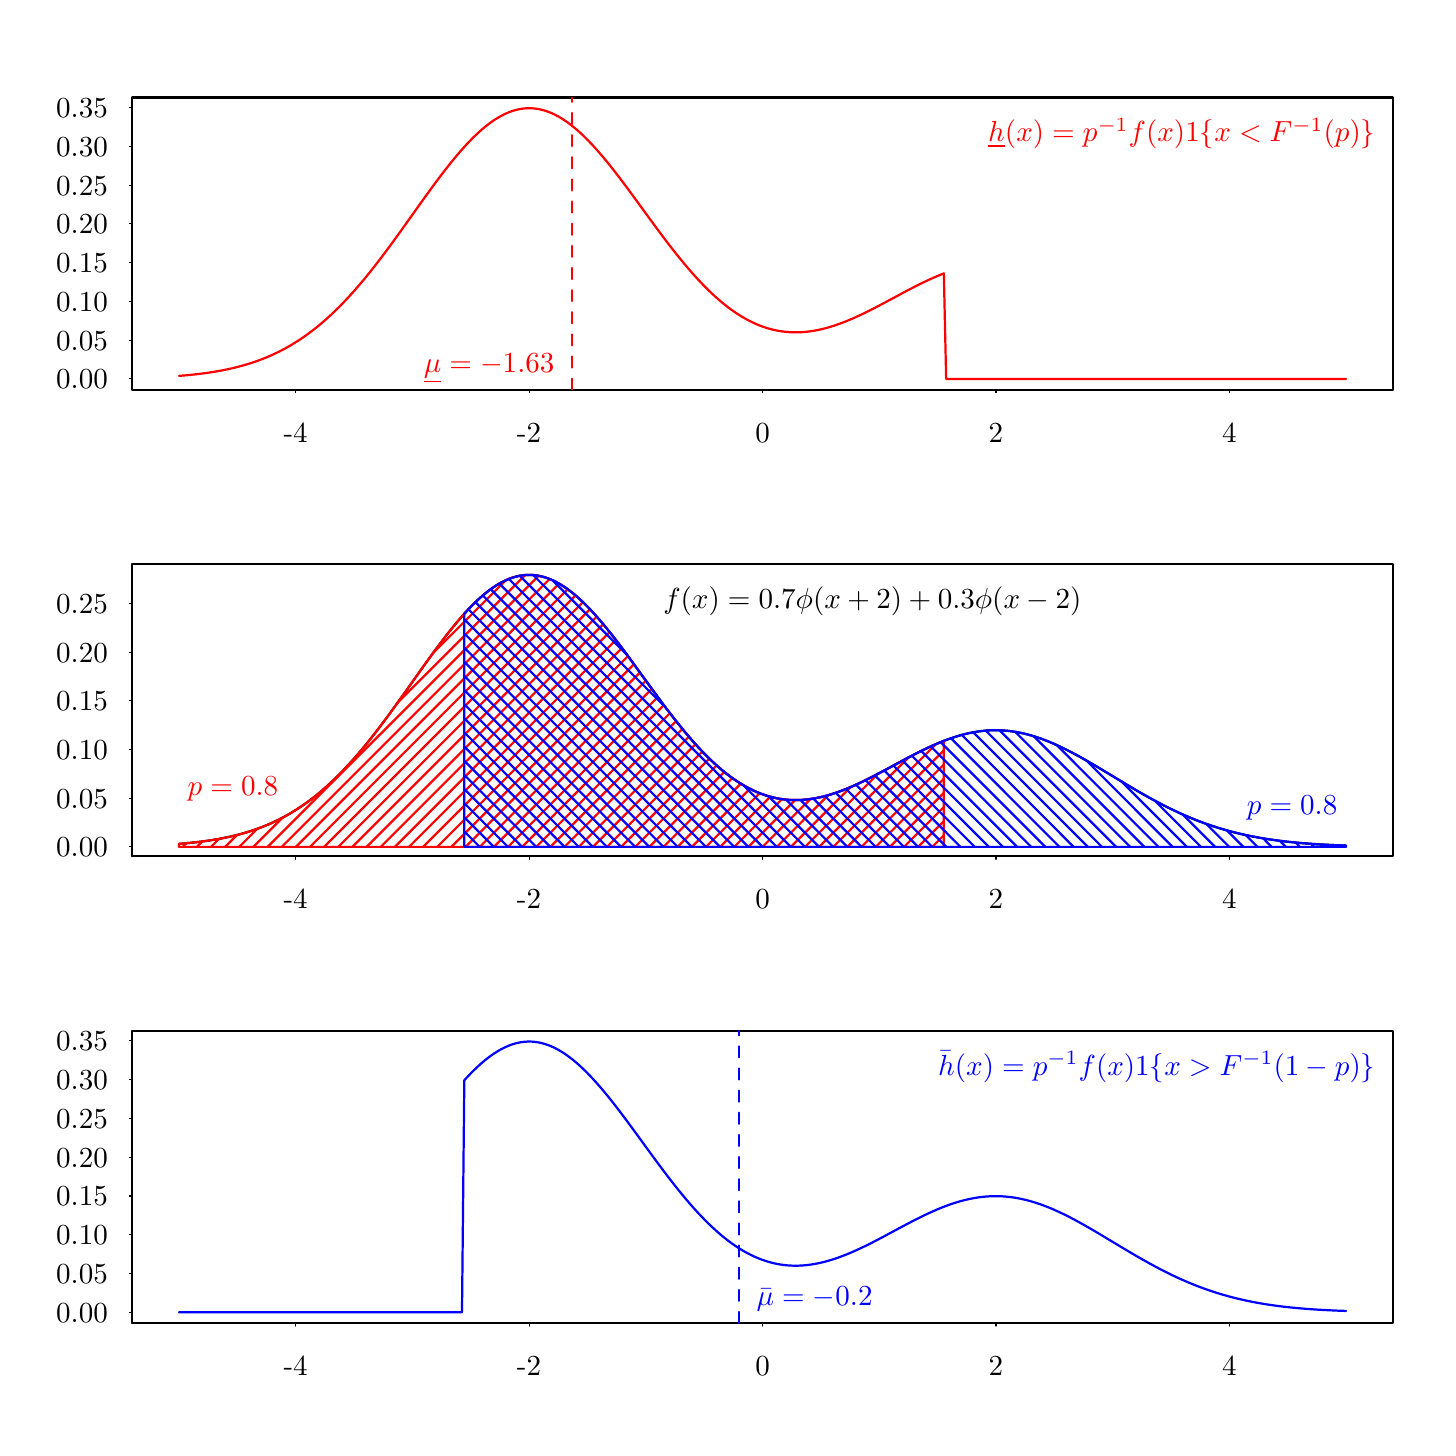
\begin{tikzpicture}[x=1pt,y=1pt]
\definecolor{fillColor}{RGB}{255,255,255}
\path[use as bounding box,fill=fillColor,fill opacity=0.00] (0,0) rectangle (505.89,505.89);
\begin{scope}
\path[clip] ( 37.80,375.06) rectangle (493.29,480.69);
\definecolor{drawColor}{RGB}{255,0,0}

\path[draw=drawColor,line width= 0.8pt,line join=round,line cap=round] ( 54.67,380.06) --
	( 55.52,380.13) --
	( 56.36,380.20) --
	( 57.21,380.27) --
	( 58.05,380.35) --
	( 58.90,380.43) --
	( 59.74,380.52) --
	( 60.59,380.61) --
	( 61.43,380.71) --
	( 62.28,380.81) --
	( 63.12,380.91) --
	( 63.97,381.03) --
	( 64.81,381.14) --
	( 65.66,381.27) --
	( 66.50,381.40) --
	( 67.35,381.53) --
	( 68.19,381.67) --
	( 69.04,381.82) --
	( 69.88,381.98) --
	( 70.73,382.14) --
	( 71.57,382.31) --
	( 72.42,382.49) --
	( 73.26,382.67) --
	( 74.11,382.87) --
	( 74.95,383.07) --
	( 75.80,383.28) --
	( 76.64,383.50) --
	( 77.49,383.73) --
	( 78.34,383.97) --
	( 79.18,384.22) --
	( 80.03,384.48) --
	( 80.87,384.75) --
	( 81.72,385.03) --
	( 82.56,385.32) --
	( 83.41,385.62) --
	( 84.25,385.94) --
	( 85.10,386.27) --
	( 85.94,386.60) --
	( 86.79,386.96) --
	( 87.63,387.32) --
	( 88.48,387.70) --
	( 89.32,388.09) --
	( 90.17,388.50) --
	( 91.01,388.91) --
	( 91.86,389.35) --
	( 92.70,389.79) --
	( 93.55,390.26) --
	( 94.39,390.73) --
	( 95.24,391.23) --
	( 96.08,391.74) --
	( 96.93,392.26) --
	( 97.77,392.80) --
	( 98.62,393.36) --
	( 99.47,393.93) --
	(100.31,394.52) --
	(101.16,395.12) --
	(102.00,395.75) --
	(102.85,396.39) --
	(103.69,397.04) --
	(104.54,397.72) --
	(105.38,398.41) --
	(106.23,399.12) --
	(107.07,399.84) --
	(107.92,400.59) --
	(108.76,401.35) --
	(109.61,402.13) --
	(110.45,402.93) --
	(111.30,403.74) --
	(112.14,404.57) --
	(112.99,405.42) --
	(113.83,406.28) --
	(114.68,407.17) --
	(115.52,408.07) --
	(116.37,408.98) --
	(117.21,409.92) --
	(118.06,410.86) --
	(118.90,411.83) --
	(119.75,412.81) --
	(120.59,413.80) --
	(121.44,414.82) --
	(122.29,415.84) --
	(123.13,416.88) --
	(123.98,417.93) --
	(124.82,419.00) --
	(125.67,420.08) --
	(126.51,421.17) --
	(127.36,422.27) --
	(128.20,423.38) --
	(129.05,424.50) --
	(129.89,425.64) --
	(130.74,426.78) --
	(131.58,427.93) --
	(132.43,429.09) --
	(133.27,430.25) --
	(134.12,431.42) --
	(134.96,432.60) --
	(135.81,433.78) --
	(136.65,434.96) --
	(137.50,436.15) --
	(138.34,437.34) --
	(139.19,438.52) --
	(140.03,439.71) --
	(140.88,440.90) --
	(141.72,442.09) --
	(142.57,443.27) --
	(143.41,444.45) --
	(144.26,445.62) --
	(145.11,446.78) --
	(145.95,447.94) --
	(146.80,449.09) --
	(147.64,450.24) --
	(148.49,451.37) --
	(149.33,452.49) --
	(150.18,453.59) --
	(151.02,454.68) --
	(151.87,455.76) --
	(152.71,456.82) --
	(153.56,457.87) --
	(154.40,458.90) --
	(155.25,459.90) --
	(156.09,460.89) --
	(156.94,461.86) --
	(157.78,462.80) --
	(158.63,463.72) --
	(159.47,464.62) --
	(160.32,465.49) --
	(161.16,466.34) --
	(162.01,467.15) --
	(162.85,467.94) --
	(163.70,468.71) --
	(164.54,469.44) --
	(165.39,470.14) --
	(166.24,470.81) --
	(167.08,471.44) --
	(167.93,472.05) --
	(168.77,472.62) --
	(169.62,473.15) --
	(170.46,473.65) --
	(171.31,474.12) --
	(172.15,474.55) --
	(173.00,474.94) --
	(173.84,475.30) --
	(174.69,475.62) --
	(175.53,475.90) --
	(176.38,476.14) --
	(177.22,476.34) --
	(178.07,476.51) --
	(178.91,476.63) --
	(179.76,476.72) --
	(180.60,476.77) --
	(181.45,476.78) --
	(182.29,476.75) --
	(183.14,476.68) --
	(183.98,476.57) --
	(184.83,476.42) --
	(185.67,476.24) --
	(186.52,476.01) --
	(187.36,475.75) --
	(188.21,475.45) --
	(189.06,475.11) --
	(189.90,474.74) --
	(190.75,474.32) --
	(191.59,473.88) --
	(192.44,473.39) --
	(193.28,472.87) --
	(194.13,472.32) --
	(194.97,471.73) --
	(195.82,471.11) --
	(196.66,470.46) --
	(197.51,469.78) --
	(198.35,469.06) --
	(199.20,468.32) --
	(200.04,467.55) --
	(200.89,466.75) --
	(201.73,465.92) --
	(202.58,465.06) --
	(203.42,464.18) --
	(204.27,463.28) --
	(205.11,462.35) --
	(205.96,461.40) --
	(206.80,460.43) --
	(207.65,459.44) --
	(208.49,458.43) --
	(209.34,457.41) --
	(210.19,456.36) --
	(211.03,455.30) --
	(211.88,454.23) --
	(212.72,453.14) --
	(213.57,452.04) --
	(214.41,450.93) --
	(215.26,449.81) --
	(216.10,448.68) --
	(216.95,447.54) --
	(217.79,446.40) --
	(218.64,445.24) --
	(219.48,444.09) --
	(220.33,442.93) --
	(221.17,441.77) --
	(222.02,440.61) --
	(222.86,439.45) --
	(223.71,438.29) --
	(224.55,437.13) --
	(225.40,435.97) --
	(226.24,434.82) --
	(227.09,433.67) --
	(227.93,432.53) --
	(228.78,431.40) --
	(229.62,430.27) --
	(230.47,429.15) --
	(231.31,428.04) --
	(232.16,426.94) --
	(233.01,425.86) --
	(233.85,424.78) --
	(234.70,423.72) --
	(235.54,422.67) --
	(236.39,421.63) --
	(237.23,420.61) --
	(238.08,419.60) --
	(238.92,418.61) --
	(239.77,417.64) --
	(240.61,416.68) --
	(241.46,415.74) --
	(242.30,414.82) --
	(243.15,413.92) --
	(243.99,413.04) --
	(244.84,412.18) --
	(245.68,411.33) --
	(246.53,410.51) --
	(247.37,409.71) --
	(248.22,408.93) --
	(249.06,408.17) --
	(249.91,407.43) --
	(250.75,406.71) --
	(251.60,406.02) --
	(252.44,405.35) --
	(253.29,404.70) --
	(254.13,404.07) --
	(254.98,403.47) --
	(255.83,402.89) --
	(256.67,402.33) --
	(257.52,401.80) --
	(258.36,401.29) --
	(259.21,400.80) --
	(260.05,400.33) --
	(260.90,399.89) --
	(261.74,399.48) --
	(262.59,399.08) --
	(263.43,398.71) --
	(264.28,398.36) --
	(265.12,398.03) --
	(265.97,397.73) --
	(266.81,397.45) --
	(267.66,397.19) --
	(268.50,396.96) --
	(269.35,396.74) --
	(270.19,396.55) --
	(271.04,396.38) --
	(271.88,396.24) --
	(272.73,396.11) --
	(273.57,396.01) --
	(274.42,395.92) --
	(275.26,395.86) --
	(276.11,395.82) --
	(276.96,395.79) --
	(277.80,395.79) --
	(278.65,395.81) --
	(279.49,395.84) --
	(280.34,395.90) --
	(281.18,395.97) --
	(282.03,396.07) --
	(282.87,396.18) --
	(283.72,396.30) --
	(284.56,396.45) --
	(285.41,396.61) --
	(286.25,396.79) --
	(287.10,396.98) --
	(287.94,397.19) --
	(288.79,397.42) --
	(289.63,397.66) --
	(290.48,397.92) --
	(291.32,398.18) --
	(292.17,398.47) --
	(293.01,398.76) --
	(293.86,399.07) --
	(294.70,399.39) --
	(295.55,399.72) --
	(296.39,400.06) --
	(297.24,400.42) --
	(298.08,400.78) --
	(298.93,401.15) --
	(299.78,401.54) --
	(300.62,401.93) --
	(301.47,402.33) --
	(302.31,402.73) --
	(303.16,403.15) --
	(304.00,403.57) --
	(304.85,403.99) --
	(305.69,404.42) --
	(306.54,404.86) --
	(307.38,405.30) --
	(308.23,405.75) --
	(309.07,406.19) --
	(309.92,406.64) --
	(310.76,407.10) --
	(311.61,407.55) --
	(312.45,408.00) --
	(313.30,408.46) --
	(314.14,408.91) --
	(314.99,409.37) --
	(315.83,409.82) --
	(316.68,410.27) --
	(317.52,410.72) --
	(318.37,411.16) --
	(319.21,411.60) --
	(320.06,412.04) --
	(320.90,412.47) --
	(321.75,412.90) --
	(322.60,413.32) --
	(323.44,413.73) --
	(324.29,414.14) --
	(325.13,414.54) --
	(325.98,414.93) --
	(326.82,415.31) --
	(327.67,415.68) --
	(328.51,416.05) --
	(329.36,416.40) --
	(330.20,416.75) --
	(331.05,417.08) --
	(331.89,378.97) --
	(332.74,378.97) --
	(333.58,378.97) --
	(334.43,378.97) --
	(335.27,378.97) --
	(336.12,378.97) --
	(336.96,378.97) --
	(337.81,378.97) --
	(338.65,378.97) --
	(339.50,378.97) --
	(340.34,378.97) --
	(341.19,378.97) --
	(342.03,378.97) --
	(342.88,378.97) --
	(343.73,378.97) --
	(344.57,378.97) --
	(345.42,378.97) --
	(346.26,378.97) --
	(347.11,378.97) --
	(347.95,378.97) --
	(348.80,378.97) --
	(349.64,378.97) --
	(350.49,378.97) --
	(351.33,378.97) --
	(352.18,378.97) --
	(353.02,378.97) --
	(353.87,378.97) --
	(354.71,378.97) --
	(355.56,378.97) --
	(356.40,378.97) --
	(357.25,378.97) --
	(358.09,378.97) --
	(358.94,378.97) --
	(359.78,378.97) --
	(360.63,378.97) --
	(361.47,378.97) --
	(362.32,378.97) --
	(363.16,378.97) --
	(364.01,378.97) --
	(364.85,378.97) --
	(365.70,378.97) --
	(366.55,378.97) --
	(367.39,378.97) --
	(368.24,378.97) --
	(369.08,378.97) --
	(369.93,378.97) --
	(370.77,378.97) --
	(371.62,378.97) --
	(372.46,378.97) --
	(373.31,378.97) --
	(374.15,378.97) --
	(375.00,378.97) --
	(375.84,378.97) --
	(376.69,378.97) --
	(377.53,378.97) --
	(378.38,378.97) --
	(379.22,378.97) --
	(380.07,378.97) --
	(380.91,378.97) --
	(381.76,378.97) --
	(382.60,378.97) --
	(383.45,378.97) --
	(384.29,378.97) --
	(385.14,378.97) --
	(385.98,378.97) --
	(386.83,378.97) --
	(387.68,378.97) --
	(388.52,378.97) --
	(389.37,378.97) --
	(390.21,378.97) --
	(391.06,378.97) --
	(391.90,378.97) --
	(392.75,378.97) --
	(393.59,378.97) --
	(394.44,378.97) --
	(395.28,378.97) --
	(396.13,378.97) --
	(396.97,378.97) --
	(397.82,378.97) --
	(398.66,378.97) --
	(399.51,378.97) --
	(400.35,378.97) --
	(401.20,378.97) --
	(402.04,378.97) --
	(402.89,378.97) --
	(403.73,378.97) --
	(404.58,378.97) --
	(405.42,378.97) --
	(406.27,378.97) --
	(407.11,378.97) --
	(407.96,378.97) --
	(408.80,378.97) --
	(409.65,378.97) --
	(410.50,378.97) --
	(411.34,378.97) --
	(412.19,378.97) --
	(413.03,378.97) --
	(413.88,378.97) --
	(414.72,378.97) --
	(415.57,378.97) --
	(416.41,378.97) --
	(417.26,378.97) --
	(418.10,378.97) --
	(418.95,378.97) --
	(419.79,378.97) --
	(420.64,378.97) --
	(421.48,378.97) --
	(422.33,378.97) --
	(423.17,378.97) --
	(424.02,378.97) --
	(424.86,378.97) --
	(425.71,378.97) --
	(426.55,378.97) --
	(427.40,378.97) --
	(428.24,378.97) --
	(429.09,378.97) --
	(429.93,378.97) --
	(430.78,378.97) --
	(431.62,378.97) --
	(432.47,378.97) --
	(433.32,378.97) --
	(434.16,378.97) --
	(435.01,378.97) --
	(435.85,378.97) --
	(436.70,378.97) --
	(437.54,378.97) --
	(438.39,378.97) --
	(439.23,378.97) --
	(440.08,378.97) --
	(440.92,378.97) --
	(441.77,378.97) --
	(442.61,378.97) --
	(443.46,378.97) --
	(444.30,378.97) --
	(445.15,378.97) --
	(445.99,378.97) --
	(446.84,378.97) --
	(447.68,378.97) --
	(448.53,378.97) --
	(449.37,378.97) --
	(450.22,378.97) --
	(451.06,378.97) --
	(451.91,378.97) --
	(452.75,378.97) --
	(453.60,378.97) --
	(454.45,378.97) --
	(455.29,378.97) --
	(456.14,378.97) --
	(456.98,378.97) --
	(457.83,378.97) --
	(458.67,378.97) --
	(459.52,378.97) --
	(460.36,378.97) --
	(461.21,378.97) --
	(462.05,378.97) --
	(462.90,378.97) --
	(463.74,378.97) --
	(464.59,378.97) --
	(465.43,378.97) --
	(466.28,378.97) --
	(467.12,378.97) --
	(467.97,378.97) --
	(468.81,378.97) --
	(469.66,378.97) --
	(470.50,378.97) --
	(471.35,378.97) --
	(472.19,378.97) --
	(473.04,378.97) --
	(473.88,378.97) --
	(474.73,378.97) --
	(475.57,378.97) --
	(476.42,378.97);
\end{scope}
\begin{scope}
\path[clip] (  0.00,  0.00) rectangle (505.89,505.89);
\definecolor{drawColor}{RGB}{0,0,0}

\path[draw=drawColor,line width= 0.4pt,line join=round,line cap=round] ( 96.84,375.06) -- (434.25,375.06);

\path[draw=drawColor,line width= 0.4pt,line join=round,line cap=round] ( 96.84,375.06) -- ( 96.84,374.00);

\path[draw=drawColor,line width= 0.4pt,line join=round,line cap=round] (181.19,375.06) -- (181.19,374.00);

\path[draw=drawColor,line width= 0.4pt,line join=round,line cap=round] (265.54,375.06) -- (265.54,374.00);

\path[draw=drawColor,line width= 0.4pt,line join=round,line cap=round] (349.89,375.06) -- (349.89,374.00);

\path[draw=drawColor,line width= 0.4pt,line join=round,line cap=round] (434.25,375.06) -- (434.25,374.00);

\node[text=drawColor,anchor=base,inner sep=0pt, outer sep=0pt, scale=  1.05] at ( 96.84,356.16) {-4};

\node[text=drawColor,anchor=base,inner sep=0pt, outer sep=0pt, scale=  1.05] at (181.19,356.16) {-2};

\node[text=drawColor,anchor=base,inner sep=0pt, outer sep=0pt, scale=  1.05] at (265.54,356.16) {0};

\node[text=drawColor,anchor=base,inner sep=0pt, outer sep=0pt, scale=  1.05] at (349.89,356.16) {2};

\node[text=drawColor,anchor=base,inner sep=0pt, outer sep=0pt, scale=  1.05] at (434.25,356.16) {4};

\path[draw=drawColor,line width= 0.4pt,line join=round,line cap=round] ( 37.80,378.97) -- ( 37.80,477.02);

\path[draw=drawColor,line width= 0.4pt,line join=round,line cap=round] ( 37.80,378.97) -- ( 36.74,378.97);

\path[draw=drawColor,line width= 0.4pt,line join=round,line cap=round] ( 37.80,392.98) -- ( 36.74,392.98);

\path[draw=drawColor,line width= 0.4pt,line join=round,line cap=round] ( 37.80,406.99) -- ( 36.74,406.99);

\path[draw=drawColor,line width= 0.4pt,line join=round,line cap=round] ( 37.80,420.99) -- ( 36.74,420.99);

\path[draw=drawColor,line width= 0.4pt,line join=round,line cap=round] ( 37.80,435.00) -- ( 36.74,435.00);

\path[draw=drawColor,line width= 0.4pt,line join=round,line cap=round] ( 37.80,449.01) -- ( 36.74,449.01);

\path[draw=drawColor,line width= 0.4pt,line join=round,line cap=round] ( 37.80,463.02) -- ( 36.74,463.02);

\path[draw=drawColor,line width= 0.4pt,line join=round,line cap=round] ( 37.80,477.02) -- ( 36.74,477.02);

\node[text=drawColor,anchor=base east,inner sep=0pt, outer sep=0pt, scale=  1.05] at ( 28.98,375.36) {0.00};

\node[text=drawColor,anchor=base east,inner sep=0pt, outer sep=0pt, scale=  1.05] at ( 28.98,389.36) {0.05};

\node[text=drawColor,anchor=base east,inner sep=0pt, outer sep=0pt, scale=  1.05] at ( 28.98,403.37) {0.10};

\node[text=drawColor,anchor=base east,inner sep=0pt, outer sep=0pt, scale=  1.05] at ( 28.98,417.38) {0.15};

\node[text=drawColor,anchor=base east,inner sep=0pt, outer sep=0pt, scale=  1.05] at ( 28.98,431.39) {0.20};

\node[text=drawColor,anchor=base east,inner sep=0pt, outer sep=0pt, scale=  1.05] at ( 28.98,445.39) {0.25};

\node[text=drawColor,anchor=base east,inner sep=0pt, outer sep=0pt, scale=  1.05] at ( 28.98,459.40) {0.30};

\node[text=drawColor,anchor=base east,inner sep=0pt, outer sep=0pt, scale=  1.05] at ( 28.98,473.41) {0.35};

\path[draw=drawColor,line width= 0.8pt,line join=round,line cap=round] ( 37.80,375.06) --
	(493.29,375.06) --
	(493.29,480.69) --
	( 37.80,480.69) --
	( 37.80,375.06);
\end{scope}
\begin{scope}
\path[clip] ( 37.80,375.06) rectangle (493.29,480.69);
\definecolor{drawColor}{RGB}{255,0,0}

\node[text=drawColor,anchor=base east,inner sep=0pt, outer sep=0pt, scale=  1.05] at (486.99,464.59) {$\underline{h}(x) = p^{-1}f(x) 1\{x < F^{-1}(p)\}$};

\path[draw=drawColor,line width= 0.8pt,dash pattern=on 4pt off 4pt ,line join=round,line cap=round] (196.63,375.06) -- (196.63,480.69);

\node[text=drawColor,anchor=base east,inner sep=0pt, outer sep=0pt, scale=  1.05] at (190.33,381.45) {$\underline{\mu} = -1.63$};
\end{scope}
\begin{scope}
\path[clip] ( 37.80,206.43) rectangle (493.29,312.06);
\definecolor{drawColor}{RGB}{0,0,0}

\path[draw=drawColor,line width= 0.8pt,line join=round,line cap=round] ( 54.67,210.97) --
	( 55.52,211.03) --
	( 56.36,211.10) --
	( 57.21,211.18) --
	( 58.05,211.26) --
	( 58.90,211.34) --
	( 59.74,211.43) --
	( 60.59,211.52) --
	( 61.43,211.62) --
	( 62.28,211.72) --
	( 63.12,211.83) --
	( 63.97,211.94) --
	( 64.81,212.06) --
	( 65.66,212.18) --
	( 66.50,212.31) --
	( 67.35,212.45) --
	( 68.19,212.59) --
	( 69.04,212.74) --
	( 69.88,212.89) --
	( 70.73,213.06) --
	( 71.57,213.23) --
	( 72.42,213.41) --
	( 73.26,213.59) --
	( 74.11,213.79) --
	( 74.95,213.99) --
	( 75.80,214.20) --
	( 76.64,214.42) --
	( 77.49,214.65) --
	( 78.34,214.90) --
	( 79.18,215.15) --
	( 80.03,215.41) --
	( 80.87,215.68) --
	( 81.72,215.96) --
	( 82.56,216.25) --
	( 83.41,216.56) --
	( 84.25,216.87) --
	( 85.10,217.20) --
	( 85.94,217.54) --
	( 86.79,217.90) --
	( 87.63,218.26) --
	( 88.48,218.64) --
	( 89.32,219.04) --
	( 90.17,219.44) --
	( 91.01,219.86) --
	( 91.86,220.30) --
	( 92.70,220.75) --
	( 93.55,221.21) --
	( 94.39,221.69) --
	( 95.24,222.19) --
	( 96.08,222.70) --
	( 96.93,223.23) --
	( 97.77,223.77) --
	( 98.62,224.33) --
	( 99.47,224.90) --
	(100.31,225.49) --
	(101.16,226.10) --
	(102.00,226.73) --
	(102.85,227.37) --
	(103.69,228.03) --
	(104.54,228.71) --
	(105.38,229.40) --
	(106.23,230.12) --
	(107.07,230.85) --
	(107.92,231.59) --
	(108.76,232.36) --
	(109.61,233.14) --
	(110.45,233.94) --
	(111.30,234.76) --
	(112.14,235.59) --
	(112.99,236.45) --
	(113.83,237.32) --
	(114.68,238.20) --
	(115.52,239.11) --
	(116.37,240.03) --
	(117.21,240.97) --
	(118.06,241.92) --
	(118.90,242.89) --
	(119.75,243.87) --
	(120.59,244.87) --
	(121.44,245.89) --
	(122.29,246.92) --
	(123.13,247.96) --
	(123.98,249.02) --
	(124.82,250.09) --
	(125.67,251.17) --
	(126.51,252.27) --
	(127.36,253.38) --
	(128.20,254.50) --
	(129.05,255.62) --
	(129.89,256.76) --
	(130.74,257.91) --
	(131.58,259.07) --
	(132.43,260.23) --
	(133.27,261.40) --
	(134.12,262.58) --
	(134.96,263.76) --
	(135.81,264.94) --
	(136.65,266.13) --
	(137.50,267.32) --
	(138.34,268.52) --
	(139.19,269.71) --
	(140.03,270.91) --
	(140.88,272.10) --
	(141.72,273.29) --
	(142.57,274.48) --
	(143.41,275.66) --
	(144.26,276.84) --
	(145.11,278.01) --
	(145.95,279.18) --
	(146.80,280.33) --
	(147.64,281.48) --
	(148.49,282.61) --
	(149.33,283.74) --
	(150.18,284.85) --
	(151.02,285.95) --
	(151.87,287.03) --
	(152.71,288.10) --
	(153.56,289.15) --
	(154.40,290.18) --
	(155.25,291.19) --
	(156.09,292.19) --
	(156.94,293.16) --
	(157.78,294.11) --
	(158.63,295.03) --
	(159.47,295.93) --
	(160.32,296.81) --
	(161.16,297.66) --
	(162.01,298.48) --
	(162.85,299.27) --
	(163.70,300.04) --
	(164.54,300.77) --
	(165.39,301.47) --
	(166.24,302.15) --
	(167.08,302.79) --
	(167.93,303.39) --
	(168.77,303.97) --
	(169.62,304.51) --
	(170.46,305.01) --
	(171.31,305.48) --
	(172.15,305.91) --
	(173.00,306.30) --
	(173.84,306.66) --
	(174.69,306.98) --
	(175.53,307.26) --
	(176.38,307.50) --
	(177.22,307.71) --
	(178.07,307.88) --
	(178.91,308.00) --
	(179.76,308.09) --
	(180.60,308.14) --
	(181.45,308.15) --
	(182.29,308.12) --
	(183.14,308.05) --
	(183.98,307.94) --
	(184.83,307.79) --
	(185.67,307.60) --
	(186.52,307.38) --
	(187.36,307.11) --
	(188.21,306.81) --
	(189.06,306.47) --
	(189.90,306.10) --
	(190.75,305.68) --
	(191.59,305.23) --
	(192.44,304.75) --
	(193.28,304.22) --
	(194.13,303.67) --
	(194.97,303.08) --
	(195.82,302.46) --
	(196.66,301.80) --
	(197.51,301.12) --
	(198.35,300.40) --
	(199.20,299.65) --
	(200.04,298.87) --
	(200.89,298.07) --
	(201.73,297.24) --
	(202.58,296.38) --
	(203.42,295.49) --
	(204.27,294.59) --
	(205.11,293.65) --
	(205.96,292.70) --
	(206.80,291.73) --
	(207.65,290.73) --
	(208.49,289.72) --
	(209.34,288.68) --
	(210.19,287.63) --
	(211.03,286.57) --
	(211.88,285.49) --
	(212.72,284.40) --
	(213.57,283.29) --
	(214.41,282.18) --
	(215.26,281.05) --
	(216.10,279.91) --
	(216.95,278.77) --
	(217.79,277.62) --
	(218.64,276.46) --
	(219.48,275.30) --
	(220.33,274.14) --
	(221.17,272.97) --
	(222.02,271.81) --
	(222.86,270.64) --
	(223.71,269.47) --
	(224.55,268.31) --
	(225.40,267.15) --
	(226.24,265.99) --
	(227.09,264.84) --
	(227.93,263.69) --
	(228.78,262.55) --
	(229.62,261.42) --
	(230.47,260.29) --
	(231.31,259.18) --
	(232.16,258.08) --
	(233.01,256.98) --
	(233.85,255.90) --
	(234.70,254.83) --
	(235.54,253.78) --
	(236.39,252.74) --
	(237.23,251.71) --
	(238.08,250.70) --
	(238.92,249.71) --
	(239.77,248.73) --
	(240.61,247.77) --
	(241.46,246.82) --
	(242.30,245.90) --
	(243.15,244.99) --
	(243.99,244.10) --
	(244.84,243.24) --
	(245.68,242.39) --
	(246.53,241.56) --
	(247.37,240.76) --
	(248.22,239.97) --
	(249.06,239.21) --
	(249.91,238.47) --
	(250.75,237.75) --
	(251.60,237.05) --
	(252.44,236.38) --
	(253.29,235.73) --
	(254.13,235.10) --
	(254.98,234.49) --
	(255.83,233.91) --
	(256.67,233.35) --
	(257.52,232.81) --
	(258.36,232.30) --
	(259.21,231.81) --
	(260.05,231.34) --
	(260.90,230.90) --
	(261.74,230.48) --
	(262.59,230.08) --
	(263.43,229.70) --
	(264.28,229.35) --
	(265.12,229.03) --
	(265.97,228.72) --
	(266.81,228.44) --
	(267.66,228.18) --
	(268.50,227.94) --
	(269.35,227.73) --
	(270.19,227.54) --
	(271.04,227.37) --
	(271.88,227.22) --
	(272.73,227.09) --
	(273.57,226.99) --
	(274.42,226.90) --
	(275.26,226.84) --
	(276.11,226.80) --
	(276.96,226.78) --
	(277.80,226.77) --
	(278.65,226.79) --
	(279.49,226.83) --
	(280.34,226.88) --
	(281.18,226.96) --
	(282.03,227.05) --
	(282.87,227.16) --
	(283.72,227.29) --
	(284.56,227.44) --
	(285.41,227.60) --
	(286.25,227.78) --
	(287.10,227.97) --
	(287.94,228.18) --
	(288.79,228.41) --
	(289.63,228.65) --
	(290.48,228.91) --
	(291.32,229.18) --
	(292.17,229.46) --
	(293.01,229.76) --
	(293.86,230.07) --
	(294.70,230.39) --
	(295.55,230.72) --
	(296.39,231.07) --
	(297.24,231.42) --
	(298.08,231.79) --
	(298.93,232.16) --
	(299.78,232.55) --
	(300.62,232.94) --
	(301.47,233.34) --
	(302.31,233.75) --
	(303.16,234.16) --
	(304.00,234.59) --
	(304.85,235.01) --
	(305.69,235.45) --
	(306.54,235.89) --
	(307.38,236.33) --
	(308.23,236.78) --
	(309.07,237.23) --
	(309.92,237.68) --
	(310.76,238.13) --
	(311.61,238.59) --
	(312.45,239.05) --
	(313.30,239.50) --
	(314.14,239.96) --
	(314.99,240.41) --
	(315.83,240.87) --
	(316.68,241.32) --
	(317.52,241.77) --
	(318.37,242.22) --
	(319.21,242.66) --
	(320.06,243.10) --
	(320.90,243.53) --
	(321.75,243.96) --
	(322.60,244.38) --
	(323.44,244.80) --
	(324.29,245.21) --
	(325.13,245.61) --
	(325.98,246.00) --
	(326.82,246.39) --
	(327.67,246.76) --
	(328.51,247.13) --
	(329.36,247.48) --
	(330.20,247.83) --
	(331.05,248.16) --
	(331.89,248.49) --
	(332.74,248.80) --
	(333.58,249.09) --
	(334.43,249.38) --
	(335.27,249.65) --
	(336.12,249.91) --
	(336.96,250.16) --
	(337.81,250.39) --
	(338.65,250.61) --
	(339.50,250.81) --
	(340.34,251.00) --
	(341.19,251.17) --
	(342.03,251.33) --
	(342.88,251.47) --
	(343.73,251.60) --
	(344.57,251.71) --
	(345.42,251.80) --
	(346.26,251.88) --
	(347.11,251.94) --
	(347.95,251.98) --
	(348.80,252.01) --
	(349.64,252.02) --
	(350.49,252.01) --
	(351.33,251.99) --
	(352.18,251.95) --
	(353.02,251.89) --
	(353.87,251.82) --
	(354.71,251.73) --
	(355.56,251.63) --
	(356.40,251.51) --
	(357.25,251.37) --
	(358.09,251.21) --
	(358.94,251.04) --
	(359.78,250.86) --
	(360.63,250.66) --
	(361.47,250.44) --
	(362.32,250.21) --
	(363.16,249.96) --
	(364.01,249.70) --
	(364.85,249.43) --
	(365.70,249.14) --
	(366.55,248.84) --
	(367.39,248.52) --
	(368.24,248.19) --
	(369.08,247.85) --
	(369.93,247.50) --
	(370.77,247.13) --
	(371.62,246.76) --
	(372.46,246.37) --
	(373.31,245.98) --
	(374.15,245.57) --
	(375.00,245.15) --
	(375.84,244.73) --
	(376.69,244.29) --
	(377.53,243.85) --
	(378.38,243.40) --
	(379.22,242.94) --
	(380.07,242.48) --
	(380.91,242.01) --
	(381.76,241.53) --
	(382.60,241.05) --
	(383.45,240.56) --
	(384.29,240.07) --
	(385.14,239.58) --
	(385.98,239.08) --
	(386.83,238.57) --
	(387.68,238.07) --
	(388.52,237.56) --
	(389.37,237.05) --
	(390.21,236.54) --
	(391.06,236.03) --
	(391.90,235.52) --
	(392.75,235.01) --
	(393.59,234.50) --
	(394.44,233.98) --
	(395.28,233.48) --
	(396.13,232.97) --
	(396.97,232.46) --
	(397.82,231.96) --
	(398.66,231.46) --
	(399.51,230.96) --
	(400.35,230.46) --
	(401.20,229.97) --
	(402.04,229.48) --
	(402.89,229.00) --
	(403.73,228.52) --
	(404.58,228.04) --
	(405.42,227.57) --
	(406.27,227.11) --
	(407.11,226.65) --
	(407.96,226.20) --
	(408.80,225.75) --
	(409.65,225.31) --
	(410.50,224.87) --
	(411.34,224.45) --
	(412.19,224.02) --
	(413.03,223.61) --
	(413.88,223.20) --
	(414.72,222.80) --
	(415.57,222.40) --
	(416.41,222.02) --
	(417.26,221.64) --
	(418.10,221.26) --
	(418.95,220.90) --
	(419.79,220.54) --
	(420.64,220.19) --
	(421.48,219.85) --
	(422.33,219.51) --
	(423.17,219.18) --
	(424.02,218.86) --
	(424.86,218.55) --
	(425.71,218.24) --
	(426.55,217.95) --
	(427.40,217.66) --
	(428.24,217.37) --
	(429.09,217.10) --
	(429.93,216.83) --
	(430.78,216.57) --
	(431.62,216.32) --
	(432.47,216.07) --
	(433.32,215.83) --
	(434.16,215.60) --
	(435.01,215.37) --
	(435.85,215.15) --
	(436.70,214.94) --
	(437.54,214.73) --
	(438.39,214.53) --
	(439.23,214.34) --
	(440.08,214.16) --
	(440.92,213.98) --
	(441.77,213.80) --
	(442.61,213.63) --
	(443.46,213.47) --
	(444.30,213.31) --
	(445.15,213.16) --
	(445.99,213.02) --
	(446.84,212.87) --
	(447.68,212.74) --
	(448.53,212.61) --
	(449.37,212.48) --
	(450.22,212.36) --
	(451.06,212.25) --
	(451.91,212.13) --
	(452.75,212.03) --
	(453.60,211.92) --
	(454.45,211.82) --
	(455.29,211.73) --
	(456.14,211.64) --
	(456.98,211.55) --
	(457.83,211.47) --
	(458.67,211.39) --
	(459.52,211.31) --
	(460.36,211.24) --
	(461.21,211.17) --
	(462.05,211.10) --
	(462.90,211.04) --
	(463.74,210.98) --
	(464.59,210.92) --
	(465.43,210.86) --
	(466.28,210.81) --
	(467.12,210.76) --
	(467.97,210.71) --
	(468.81,210.67) --
	(469.66,210.62) --
	(470.50,210.58) --
	(471.35,210.54) --
	(472.19,210.50) --
	(473.04,210.47) --
	(473.88,210.43) --
	(474.73,210.40) --
	(475.57,210.37) --
	(476.42,210.34);
\end{scope}
\begin{scope}
\path[clip] (  0.00,  0.00) rectangle (505.89,505.89);
\definecolor{drawColor}{RGB}{0,0,0}

\path[draw=drawColor,line width= 0.4pt,line join=round,line cap=round] ( 96.84,206.43) -- (434.25,206.43);

\path[draw=drawColor,line width= 0.4pt,line join=round,line cap=round] ( 96.84,206.43) -- ( 96.84,205.37);

\path[draw=drawColor,line width= 0.4pt,line join=round,line cap=round] (181.19,206.43) -- (181.19,205.37);

\path[draw=drawColor,line width= 0.4pt,line join=round,line cap=round] (265.54,206.43) -- (265.54,205.37);

\path[draw=drawColor,line width= 0.4pt,line join=round,line cap=round] (349.89,206.43) -- (349.89,205.37);

\path[draw=drawColor,line width= 0.4pt,line join=round,line cap=round] (434.25,206.43) -- (434.25,205.37);

\node[text=drawColor,anchor=base,inner sep=0pt, outer sep=0pt, scale=  1.05] at ( 96.84,187.53) {-4};

\node[text=drawColor,anchor=base,inner sep=0pt, outer sep=0pt, scale=  1.05] at (181.19,187.53) {-2};

\node[text=drawColor,anchor=base,inner sep=0pt, outer sep=0pt, scale=  1.05] at (265.54,187.53) {0};

\node[text=drawColor,anchor=base,inner sep=0pt, outer sep=0pt, scale=  1.05] at (349.89,187.53) {2};

\node[text=drawColor,anchor=base,inner sep=0pt, outer sep=0pt, scale=  1.05] at (434.25,187.53) {4};

\path[draw=drawColor,line width= 0.4pt,line join=round,line cap=round] ( 37.80,209.87) -- ( 37.80,297.84);

\path[draw=drawColor,line width= 0.4pt,line join=round,line cap=round] ( 37.80,209.87) -- ( 36.74,209.87);

\path[draw=drawColor,line width= 0.4pt,line join=round,line cap=round] ( 37.80,227.47) -- ( 36.74,227.47);

\path[draw=drawColor,line width= 0.4pt,line join=round,line cap=round] ( 37.80,245.06) -- ( 36.74,245.06);

\path[draw=drawColor,line width= 0.4pt,line join=round,line cap=round] ( 37.80,262.65) -- ( 36.74,262.65);

\path[draw=drawColor,line width= 0.4pt,line join=round,line cap=round] ( 37.80,280.25) -- ( 36.74,280.25);

\path[draw=drawColor,line width= 0.4pt,line join=round,line cap=round] ( 37.80,297.84) -- ( 36.74,297.84);

\node[text=drawColor,anchor=base east,inner sep=0pt, outer sep=0pt, scale=  1.05] at ( 28.98,206.26) {0.00};

\node[text=drawColor,anchor=base east,inner sep=0pt, outer sep=0pt, scale=  1.05] at ( 28.98,223.85) {0.05};

\node[text=drawColor,anchor=base east,inner sep=0pt, outer sep=0pt, scale=  1.05] at ( 28.98,241.44) {0.10};

\node[text=drawColor,anchor=base east,inner sep=0pt, outer sep=0pt, scale=  1.05] at ( 28.98,259.04) {0.15};

\node[text=drawColor,anchor=base east,inner sep=0pt, outer sep=0pt, scale=  1.05] at ( 28.98,276.63) {0.20};

\node[text=drawColor,anchor=base east,inner sep=0pt, outer sep=0pt, scale=  1.05] at ( 28.98,294.22) {0.25};

\path[draw=drawColor,line width= 0.8pt,line join=round,line cap=round] ( 37.80,206.43) --
	(493.29,206.43) --
	(493.29,312.06) --
	( 37.80,312.06) --
	( 37.80,206.43);
\end{scope}
\begin{scope}
\path[clip] ( 37.80,206.43) rectangle (493.29,312.06);
\definecolor{drawColor}{RGB}{255,0,0}

\path[draw=drawColor,line width= 0.8pt,line join=round,line cap=round] ( 56.02,209.87) -- ( 57.34,211.19);

\path[draw=drawColor,line width= 0.8pt,line join=round,line cap=round] ( 61.13,209.87) -- ( 63.08,211.82);

\path[draw=drawColor,line width= 0.8pt,line join=round,line cap=round] ( 66.24,209.87) -- ( 69.12,212.75);

\path[draw=drawColor,line width= 0.8pt,line join=round,line cap=round] ( 71.36,209.87) -- ( 75.64,214.16);

\path[draw=drawColor,line width= 0.8pt,line join=round,line cap=round] ( 76.47,209.87) -- ( 83.00,216.41);

\path[draw=drawColor,line width= 0.8pt,line join=round,line cap=round] (146.45,279.86) -- (172.80,306.21);

\path[draw=drawColor,line width= 0.8pt,line join=round,line cap=round] ( 81.58,209.87) -- ( 92.16,220.46);

\path[draw=drawColor,line width= 0.8pt,line join=round,line cap=round] (133.71,262.01) -- (179.79,308.09);

\path[draw=drawColor,line width= 0.8pt,line join=round,line cap=round] ( 86.69,209.87) -- (184.64,307.82);

\path[draw=drawColor,line width= 0.8pt,line join=round,line cap=round] ( 91.80,209.87) -- (188.58,306.66);

\path[draw=drawColor,line width= 0.8pt,line join=round,line cap=round] ( 96.91,209.87) -- (192.02,304.99);

\path[draw=drawColor,line width= 0.8pt,line join=round,line cap=round] (102.02,209.87) -- (195.12,302.97);

\path[draw=drawColor,line width= 0.8pt,line join=round,line cap=round] (107.13,209.87) -- (197.97,300.72);

\path[draw=drawColor,line width= 0.8pt,line join=round,line cap=round] (112.24,209.87) -- (200.65,298.29);

\path[draw=drawColor,line width= 0.8pt,line join=round,line cap=round] (117.35,209.87) -- (203.20,295.73);

\path[draw=drawColor,line width= 0.8pt,line join=round,line cap=round] (122.46,209.87) -- (205.64,293.06);

\path[draw=drawColor,line width= 0.8pt,line join=round,line cap=round] (127.57,209.87) -- (208.00,290.31);

\path[draw=drawColor,line width= 0.8pt,line join=round,line cap=round] (132.68,209.87) -- (210.30,287.49);

\path[draw=drawColor,line width= 0.8pt,line join=round,line cap=round] (137.79,209.87) -- (212.54,284.63);

\path[draw=drawColor,line width= 0.8pt,line join=round,line cap=round] (142.90,209.87) -- (214.75,281.72);

\path[draw=drawColor,line width= 0.8pt,line join=round,line cap=round] (148.01,209.87) -- (216.93,278.79);

\path[draw=drawColor,line width= 0.8pt,line join=round,line cap=round] (153.12,209.87) -- (219.09,275.84);

\path[draw=drawColor,line width= 0.8pt,line join=round,line cap=round] (158.23,209.87) -- (221.24,272.88);

\path[draw=drawColor,line width= 0.8pt,line join=round,line cap=round] (163.34,209.87) -- (223.39,269.92);

\path[draw=drawColor,line width= 0.8pt,line join=round,line cap=round] (168.45,209.87) -- (225.54,266.96);

\path[draw=drawColor,line width= 0.8pt,line join=round,line cap=round] (173.56,209.87) -- (227.70,264.01);

\path[draw=drawColor,line width= 0.8pt,line join=round,line cap=round] (178.67,209.87) -- (229.88,261.08);

\path[draw=drawColor,line width= 0.8pt,line join=round,line cap=round] (183.78,209.87) -- (232.08,258.18);

\path[draw=drawColor,line width= 0.8pt,line join=round,line cap=round] (188.89,209.87) -- (234.32,255.31);

\path[draw=drawColor,line width= 0.8pt,line join=round,line cap=round] (194.00,209.87) -- (236.60,252.47);

\path[draw=drawColor,line width= 0.8pt,line join=round,line cap=round] (199.11,209.87) -- (238.93,249.69);

\path[draw=drawColor,line width= 0.8pt,line join=round,line cap=round] (204.22,209.87) -- (241.32,246.97);

\path[draw=drawColor,line width= 0.8pt,line join=round,line cap=round] (209.33,209.87) -- (243.78,244.32);

\path[draw=drawColor,line width= 0.8pt,line join=round,line cap=round] (214.44,209.87) -- (246.33,241.76);

\path[draw=drawColor,line width= 0.8pt,line join=round,line cap=round] (219.55,209.87) -- (248.97,239.29);

\path[draw=drawColor,line width= 0.8pt,line join=round,line cap=round] (224.66,209.87) -- (251.73,236.95);

\path[draw=drawColor,line width= 0.8pt,line join=round,line cap=round] (229.77,209.87) -- (254.64,234.74);

\path[draw=drawColor,line width= 0.8pt,line join=round,line cap=round] (234.88,209.87) -- (257.70,232.70);

\path[draw=drawColor,line width= 0.8pt,line join=round,line cap=round] (239.99,209.87) -- (260.98,230.86);

\path[draw=drawColor,line width= 0.8pt,line join=round,line cap=round] (245.10,209.87) -- (264.50,229.27);

\path[draw=drawColor,line width= 0.8pt,line join=round,line cap=round] (250.21,209.87) -- (268.33,227.99);

\path[draw=drawColor,line width= 0.8pt,line join=round,line cap=round] (255.32,209.87) -- (272.57,227.12);

\path[draw=drawColor,line width= 0.8pt,line join=round,line cap=round] (260.43,209.87) -- (277.34,226.77);

\path[draw=drawColor,line width= 0.8pt,line join=round,line cap=round] (265.54,209.87) -- (282.83,227.15);

\path[draw=drawColor,line width= 0.8pt,line join=round,line cap=round] (270.66,209.87) -- (289.35,228.57);

\path[draw=drawColor,line width= 0.8pt,line join=round,line cap=round] (275.77,209.87) -- (297.37,231.48);

\path[draw=drawColor,line width= 0.8pt,line join=round,line cap=round] (280.88,209.87) -- (307.28,236.27);

\path[draw=drawColor,line width= 0.8pt,line join=round,line cap=round] (285.99,209.87) -- (318.28,242.17);

\path[draw=drawColor,line width= 0.8pt,line join=round,line cap=round] (291.10,209.87) -- (328.22,247.00);

\path[draw=drawColor,line width= 0.8pt,line join=round,line cap=round] (296.21,209.87) -- (331.05,244.72);

\path[draw=drawColor,line width= 0.8pt,line join=round,line cap=round] (301.32,209.87) -- (331.05,239.60);

\path[draw=drawColor,line width= 0.8pt,line join=round,line cap=round] (306.43,209.87) -- (331.05,234.49);

\path[draw=drawColor,line width= 0.8pt,line join=round,line cap=round] (311.54,209.87) -- (331.05,229.38);

\path[draw=drawColor,line width= 0.8pt,line join=round,line cap=round] (316.65,209.87) -- (331.05,224.27);

\path[draw=drawColor,line width= 0.8pt,line join=round,line cap=round] (321.76,209.87) -- (331.05,219.16);

\path[draw=drawColor,line width= 0.8pt,line join=round,line cap=round] (326.87,209.87) -- (331.05,214.05);

\path[draw=drawColor,line width= 0.8pt,line join=round,line cap=round] ( 54.67,209.87) --
	( 55.52,209.87) --
	( 56.36,209.87) --
	( 57.21,209.87) --
	( 58.05,209.87) --
	( 58.90,209.87) --
	( 59.74,209.87) --
	( 60.59,209.87) --
	( 61.43,209.87) --
	( 62.28,209.87) --
	( 63.12,209.87) --
	( 63.97,209.87) --
	( 64.81,209.87) --
	( 65.66,209.87) --
	( 66.50,209.87) --
	( 67.35,209.87) --
	( 68.19,209.87) --
	( 69.04,209.87) --
	( 69.88,209.87) --
	( 70.73,209.87) --
	( 71.57,209.87) --
	( 72.42,209.87) --
	( 73.26,209.87) --
	( 74.11,209.87) --
	( 74.95,209.87) --
	( 75.80,209.87) --
	( 76.64,209.87) --
	( 77.49,209.87) --
	( 78.34,209.87) --
	( 79.18,209.87) --
	( 80.03,209.87) --
	( 80.87,209.87) --
	( 81.72,209.87) --
	( 82.56,209.87) --
	( 83.41,209.87) --
	( 84.25,209.87) --
	( 85.10,209.87) --
	( 85.94,209.87) --
	( 86.79,209.87) --
	( 87.63,209.87) --
	( 88.48,209.87) --
	( 89.32,209.87) --
	( 90.17,209.87) --
	( 91.01,209.87) --
	( 91.86,209.87) --
	( 92.70,209.87) --
	( 93.55,209.87) --
	( 94.39,209.87) --
	( 95.24,209.87) --
	( 96.08,209.87) --
	( 96.93,209.87) --
	( 97.77,209.87) --
	( 98.62,209.87) --
	( 99.47,209.87) --
	(100.31,209.87) --
	(101.16,209.87) --
	(102.00,209.87) --
	(102.85,209.87) --
	(103.69,209.87) --
	(104.54,209.87) --
	(105.38,209.87) --
	(106.23,209.87) --
	(107.07,209.87) --
	(107.92,209.87) --
	(108.76,209.87) --
	(109.61,209.87) --
	(110.45,209.87) --
	(111.30,209.87) --
	(112.14,209.87) --
	(112.99,209.87) --
	(113.83,209.87) --
	(114.68,209.87) --
	(115.52,209.87) --
	(116.37,209.87) --
	(117.21,209.87) --
	(118.06,209.87) --
	(118.90,209.87) --
	(119.75,209.87) --
	(120.59,209.87) --
	(121.44,209.87) --
	(122.29,209.87) --
	(123.13,209.87) --
	(123.98,209.87) --
	(124.82,209.87) --
	(125.67,209.87) --
	(126.51,209.87) --
	(127.36,209.87) --
	(128.20,209.87) --
	(129.05,209.87) --
	(129.89,209.87) --
	(130.74,209.87) --
	(131.58,209.87) --
	(132.43,209.87) --
	(133.27,209.87) --
	(134.12,209.87) --
	(134.96,209.87) --
	(135.81,209.87) --
	(136.65,209.87) --
	(137.50,209.87) --
	(138.34,209.87) --
	(139.19,209.87) --
	(140.03,209.87) --
	(140.88,209.87) --
	(141.72,209.87) --
	(142.57,209.87) --
	(143.41,209.87) --
	(144.26,209.87) --
	(145.11,209.87) --
	(145.95,209.87) --
	(146.80,209.87) --
	(147.64,209.87) --
	(148.49,209.87) --
	(149.33,209.87) --
	(150.18,209.87) --
	(151.02,209.87) --
	(151.87,209.87) --
	(152.71,209.87) --
	(153.56,209.87) --
	(154.40,209.87) --
	(155.25,209.87) --
	(156.09,209.87) --
	(156.94,209.87) --
	(157.78,209.87) --
	(158.63,209.87) --
	(159.47,209.87) --
	(160.32,209.87) --
	(161.16,209.87) --
	(162.01,209.87) --
	(162.85,209.87) --
	(163.70,209.87) --
	(164.54,209.87) --
	(165.39,209.87) --
	(166.24,209.87) --
	(167.08,209.87) --
	(167.93,209.87) --
	(168.77,209.87) --
	(169.62,209.87) --
	(170.46,209.87) --
	(171.31,209.87) --
	(172.15,209.87) --
	(173.00,209.87) --
	(173.84,209.87) --
	(174.69,209.87) --
	(175.53,209.87) --
	(176.38,209.87) --
	(177.22,209.87) --
	(178.07,209.87) --
	(178.91,209.87) --
	(179.76,209.87) --
	(180.60,209.87) --
	(181.45,209.87) --
	(182.29,209.87) --
	(183.14,209.87) --
	(183.98,209.87) --
	(184.83,209.87) --
	(185.67,209.87) --
	(186.52,209.87) --
	(187.36,209.87) --
	(188.21,209.87) --
	(189.06,209.87) --
	(189.90,209.87) --
	(190.75,209.87) --
	(191.59,209.87) --
	(192.44,209.87) --
	(193.28,209.87) --
	(194.13,209.87) --
	(194.97,209.87) --
	(195.82,209.87) --
	(196.66,209.87) --
	(197.51,209.87) --
	(198.35,209.87) --
	(199.20,209.87) --
	(200.04,209.87) --
	(200.89,209.87) --
	(201.73,209.87) --
	(202.58,209.87) --
	(203.42,209.87) --
	(204.27,209.87) --
	(205.11,209.87) --
	(205.96,209.87) --
	(206.80,209.87) --
	(207.65,209.87) --
	(208.49,209.87) --
	(209.34,209.87) --
	(210.19,209.87) --
	(211.03,209.87) --
	(211.88,209.87) --
	(212.72,209.87) --
	(213.57,209.87) --
	(214.41,209.87) --
	(215.26,209.87) --
	(216.10,209.87) --
	(216.95,209.87) --
	(217.79,209.87) --
	(218.64,209.87) --
	(219.48,209.87) --
	(220.33,209.87) --
	(221.17,209.87) --
	(222.02,209.87) --
	(222.86,209.87) --
	(223.71,209.87) --
	(224.55,209.87) --
	(225.40,209.87) --
	(226.24,209.87) --
	(227.09,209.87) --
	(227.93,209.87) --
	(228.78,209.87) --
	(229.62,209.87) --
	(230.47,209.87) --
	(231.31,209.87) --
	(232.16,209.87) --
	(233.01,209.87) --
	(233.85,209.87) --
	(234.70,209.87) --
	(235.54,209.87) --
	(236.39,209.87) --
	(237.23,209.87) --
	(238.08,209.87) --
	(238.92,209.87) --
	(239.77,209.87) --
	(240.61,209.87) --
	(241.46,209.87) --
	(242.30,209.87) --
	(243.15,209.87) --
	(243.99,209.87) --
	(244.84,209.87) --
	(245.68,209.87) --
	(246.53,209.87) --
	(247.37,209.87) --
	(248.22,209.87) --
	(249.06,209.87) --
	(249.91,209.87) --
	(250.75,209.87) --
	(251.60,209.87) --
	(252.44,209.87) --
	(253.29,209.87) --
	(254.13,209.87) --
	(254.98,209.87) --
	(255.83,209.87) --
	(256.67,209.87) --
	(257.52,209.87) --
	(258.36,209.87) --
	(259.21,209.87) --
	(260.05,209.87) --
	(260.90,209.87) --
	(261.74,209.87) --
	(262.59,209.87) --
	(263.43,209.87) --
	(264.28,209.87) --
	(265.12,209.87) --
	(265.97,209.87) --
	(266.81,209.87) --
	(267.66,209.87) --
	(268.50,209.87) --
	(269.35,209.87) --
	(270.19,209.87) --
	(271.04,209.87) --
	(271.88,209.87) --
	(272.73,209.87) --
	(273.57,209.87) --
	(274.42,209.87) --
	(275.26,209.87) --
	(276.11,209.87) --
	(276.96,209.87) --
	(277.80,209.87) --
	(278.65,209.87) --
	(279.49,209.87) --
	(280.34,209.87) --
	(281.18,209.87) --
	(282.03,209.87) --
	(282.87,209.87) --
	(283.72,209.87) --
	(284.56,209.87) --
	(285.41,209.87) --
	(286.25,209.87) --
	(287.10,209.87) --
	(287.94,209.87) --
	(288.79,209.87) --
	(289.63,209.87) --
	(290.48,209.87) --
	(291.32,209.87) --
	(292.17,209.87) --
	(293.01,209.87) --
	(293.86,209.87) --
	(294.70,209.87) --
	(295.55,209.87) --
	(296.39,209.87) --
	(297.24,209.87) --
	(298.08,209.87) --
	(298.93,209.87) --
	(299.78,209.87) --
	(300.62,209.87) --
	(301.47,209.87) --
	(302.31,209.87) --
	(303.16,209.87) --
	(304.00,209.87) --
	(304.85,209.87) --
	(305.69,209.87) --
	(306.54,209.87) --
	(307.38,209.87) --
	(308.23,209.87) --
	(309.07,209.87) --
	(309.92,209.87) --
	(310.76,209.87) --
	(311.61,209.87) --
	(312.45,209.87) --
	(313.30,209.87) --
	(314.14,209.87) --
	(314.99,209.87) --
	(315.83,209.87) --
	(316.68,209.87) --
	(317.52,209.87) --
	(318.37,209.87) --
	(319.21,209.87) --
	(320.06,209.87) --
	(320.90,209.87) --
	(321.75,209.87) --
	(322.60,209.87) --
	(323.44,209.87) --
	(324.29,209.87) --
	(325.13,209.87) --
	(325.98,209.87) --
	(326.82,209.87) --
	(327.67,209.87) --
	(328.51,209.87) --
	(329.36,209.87) --
	(330.20,209.87) --
	(331.05,209.87) --
	(331.05,248.16) --
	(330.20,247.83) --
	(329.36,247.48) --
	(328.51,247.13) --
	(327.67,246.76) --
	(326.82,246.39) --
	(325.98,246.00) --
	(325.13,245.61) --
	(324.29,245.21) --
	(323.44,244.80) --
	(322.60,244.38) --
	(321.75,243.96) --
	(320.90,243.53) --
	(320.06,243.10) --
	(319.21,242.66) --
	(318.37,242.22) --
	(317.52,241.77) --
	(316.68,241.32) --
	(315.83,240.87) --
	(314.99,240.41) --
	(314.14,239.96) --
	(313.30,239.50) --
	(312.45,239.05) --
	(311.61,238.59) --
	(310.76,238.13) --
	(309.92,237.68) --
	(309.07,237.23) --
	(308.23,236.78) --
	(307.38,236.33) --
	(306.54,235.89) --
	(305.69,235.45) --
	(304.85,235.01) --
	(304.00,234.59) --
	(303.16,234.16) --
	(302.31,233.75) --
	(301.47,233.34) --
	(300.62,232.94) --
	(299.78,232.55) --
	(298.93,232.16) --
	(298.08,231.79) --
	(297.24,231.42) --
	(296.39,231.07) --
	(295.55,230.72) --
	(294.70,230.39) --
	(293.86,230.07) --
	(293.01,229.76) --
	(292.17,229.46) --
	(291.32,229.18) --
	(290.48,228.91) --
	(289.63,228.65) --
	(288.79,228.41) --
	(287.94,228.18) --
	(287.10,227.97) --
	(286.25,227.78) --
	(285.41,227.60) --
	(284.56,227.44) --
	(283.72,227.29) --
	(282.87,227.16) --
	(282.03,227.05) --
	(281.18,226.96) --
	(280.34,226.88) --
	(279.49,226.83) --
	(278.65,226.79) --
	(277.80,226.77) --
	(276.96,226.78) --
	(276.11,226.80) --
	(275.26,226.84) --
	(274.42,226.90) --
	(273.57,226.99) --
	(272.73,227.09) --
	(271.88,227.22) --
	(271.04,227.37) --
	(270.19,227.54) --
	(269.35,227.73) --
	(268.50,227.94) --
	(267.66,228.18) --
	(266.81,228.44) --
	(265.97,228.72) --
	(265.12,229.03) --
	(264.28,229.35) --
	(263.43,229.70) --
	(262.59,230.08) --
	(261.74,230.48) --
	(260.90,230.90) --
	(260.05,231.34) --
	(259.21,231.81) --
	(258.36,232.30) --
	(257.52,232.81) --
	(256.67,233.35) --
	(255.83,233.91) --
	(254.98,234.49) --
	(254.13,235.10) --
	(253.29,235.73) --
	(252.44,236.38) --
	(251.60,237.05) --
	(250.75,237.75) --
	(249.91,238.47) --
	(249.06,239.21) --
	(248.22,239.97) --
	(247.37,240.76) --
	(246.53,241.56) --
	(245.68,242.39) --
	(244.84,243.24) --
	(243.99,244.10) --
	(243.15,244.99) --
	(242.30,245.90) --
	(241.46,246.82) --
	(240.61,247.77) --
	(239.77,248.73) --
	(238.92,249.71) --
	(238.08,250.70) --
	(237.23,251.71) --
	(236.39,252.74) --
	(235.54,253.78) --
	(234.70,254.83) --
	(233.85,255.90) --
	(233.01,256.98) --
	(232.16,258.08) --
	(231.31,259.18) --
	(230.47,260.29) --
	(229.62,261.42) --
	(228.78,262.55) --
	(227.93,263.69) --
	(227.09,264.84) --
	(226.24,265.99) --
	(225.40,267.15) --
	(224.55,268.31) --
	(223.71,269.47) --
	(222.86,270.64) --
	(222.02,271.81) --
	(221.17,272.97) --
	(220.33,274.14) --
	(219.48,275.30) --
	(218.64,276.46) --
	(217.79,277.62) --
	(216.95,278.77) --
	(216.10,279.91) --
	(215.26,281.05) --
	(214.41,282.18) --
	(213.57,283.29) --
	(212.72,284.40) --
	(211.88,285.49) --
	(211.03,286.57) --
	(210.19,287.63) --
	(209.34,288.68) --
	(208.49,289.72) --
	(207.65,290.73) --
	(206.80,291.73) --
	(205.96,292.70) --
	(205.11,293.65) --
	(204.27,294.59) --
	(203.42,295.49) --
	(202.58,296.38) --
	(201.73,297.24) --
	(200.89,298.07) --
	(200.04,298.87) --
	(199.20,299.65) --
	(198.35,300.40) --
	(197.51,301.12) --
	(196.66,301.80) --
	(195.82,302.46) --
	(194.97,303.08) --
	(194.13,303.67) --
	(193.28,304.22) --
	(192.44,304.75) --
	(191.59,305.23) --
	(190.75,305.68) --
	(189.90,306.10) --
	(189.06,306.47) --
	(188.21,306.81) --
	(187.36,307.11) --
	(186.52,307.38) --
	(185.67,307.60) --
	(184.83,307.79) --
	(183.98,307.94) --
	(183.14,308.05) --
	(182.29,308.12) --
	(181.45,308.15) --
	(180.60,308.14) --
	(179.76,308.09) --
	(178.91,308.00) --
	(178.07,307.88) --
	(177.22,307.71) --
	(176.38,307.50) --
	(175.53,307.26) --
	(174.69,306.98) --
	(173.84,306.66) --
	(173.00,306.30) --
	(172.15,305.91) --
	(171.31,305.48) --
	(170.46,305.01) --
	(169.62,304.51) --
	(168.77,303.97) --
	(167.93,303.39) --
	(167.08,302.79) --
	(166.24,302.15) --
	(165.39,301.47) --
	(164.54,300.77) --
	(163.70,300.04) --
	(162.85,299.27) --
	(162.01,298.48) --
	(161.16,297.66) --
	(160.32,296.81) --
	(159.47,295.93) --
	(158.63,295.03) --
	(157.78,294.11) --
	(156.94,293.16) --
	(156.09,292.19) --
	(155.25,291.19) --
	(154.40,290.18) --
	(153.56,289.15) --
	(152.71,288.10) --
	(151.87,287.03) --
	(151.02,285.95) --
	(150.18,284.85) --
	(149.33,283.74) --
	(148.49,282.61) --
	(147.64,281.48) --
	(146.80,280.33) --
	(145.95,279.18) --
	(145.11,278.01) --
	(144.26,276.84) --
	(143.41,275.66) --
	(142.57,274.48) --
	(141.72,273.29) --
	(140.88,272.10) --
	(140.03,270.91) --
	(139.19,269.71) --
	(138.34,268.52) --
	(137.50,267.32) --
	(136.65,266.13) --
	(135.81,264.94) --
	(134.96,263.76) --
	(134.12,262.58) --
	(133.27,261.40) --
	(132.43,260.23) --
	(131.58,259.07) --
	(130.74,257.91) --
	(129.89,256.76) --
	(129.05,255.62) --
	(128.20,254.50) --
	(127.36,253.38) --
	(126.51,252.27) --
	(125.67,251.17) --
	(124.82,250.09) --
	(123.98,249.02) --
	(123.13,247.96) --
	(122.29,246.92) --
	(121.44,245.89) --
	(120.59,244.87) --
	(119.75,243.87) --
	(118.90,242.89) --
	(118.06,241.92) --
	(117.21,240.97) --
	(116.37,240.03) --
	(115.52,239.11) --
	(114.68,238.20) --
	(113.83,237.32) --
	(112.99,236.45) --
	(112.14,235.59) --
	(111.30,234.76) --
	(110.45,233.94) --
	(109.61,233.14) --
	(108.76,232.36) --
	(107.92,231.59) --
	(107.07,230.85) --
	(106.23,230.12) --
	(105.38,229.40) --
	(104.54,228.71) --
	(103.69,228.03) --
	(102.85,227.37) --
	(102.00,226.73) --
	(101.16,226.10) --
	(100.31,225.49) --
	( 99.47,224.90) --
	( 98.62,224.33) --
	( 97.77,223.77) --
	( 96.93,223.23) --
	( 96.08,222.70) --
	( 95.24,222.19) --
	( 94.39,221.69) --
	( 93.55,221.21) --
	( 92.70,220.75) --
	( 91.86,220.30) --
	( 91.01,219.86) --
	( 90.17,219.44) --
	( 89.32,219.04) --
	( 88.48,218.64) --
	( 87.63,218.26) --
	( 86.79,217.90) --
	( 85.94,217.54) --
	( 85.10,217.20) --
	( 84.25,216.87) --
	( 83.41,216.56) --
	( 82.56,216.25) --
	( 81.72,215.96) --
	( 80.87,215.68) --
	( 80.03,215.41) --
	( 79.18,215.15) --
	( 78.34,214.90) --
	( 77.49,214.65) --
	( 76.64,214.42) --
	( 75.80,214.20) --
	( 74.95,213.99) --
	( 74.11,213.79) --
	( 73.26,213.59) --
	( 72.42,213.41) --
	( 71.57,213.23) --
	( 70.73,213.06) --
	( 69.88,212.89) --
	( 69.04,212.74) --
	( 68.19,212.59) --
	( 67.35,212.45) --
	( 66.50,212.31) --
	( 65.66,212.18) --
	( 64.81,212.06) --
	( 63.97,211.94) --
	( 63.12,211.83) --
	( 62.28,211.72) --
	( 61.43,211.62) --
	( 60.59,211.52) --
	( 59.74,211.43) --
	( 58.90,211.34) --
	( 58.05,211.26) --
	( 57.21,211.18) --
	( 56.36,211.10) --
	( 55.52,211.03) --
	( 54.67,210.97) --
	( 54.67,209.87);

\node[text=drawColor,anchor=base east,inner sep=0pt, outer sep=0pt, scale=  1.05] at ( 90.54,228.58) {$p = 0.8$};
\definecolor{drawColor}{RGB}{0,0,255}

\path[draw=drawColor,line width= 0.8pt,line join=round,line cap=round] (158.23,209.87) -- (157.78,210.32);

\path[draw=drawColor,line width= 0.8pt,line join=round,line cap=round] (163.34,209.87) -- (157.78,215.43);

\path[draw=drawColor,line width= 0.8pt,line join=round,line cap=round] (168.45,209.87) -- (157.78,220.54);

\path[draw=drawColor,line width= 0.8pt,line join=round,line cap=round] (173.56,209.87) -- (157.78,225.65);

\path[draw=drawColor,line width= 0.8pt,line join=round,line cap=round] (178.67,209.87) -- (157.78,230.76);

\path[draw=drawColor,line width= 0.8pt,line join=round,line cap=round] (183.78,209.87) -- (157.78,235.87);

\path[draw=drawColor,line width= 0.8pt,line join=round,line cap=round] (188.89,209.87) -- (157.78,240.98);

\path[draw=drawColor,line width= 0.8pt,line join=round,line cap=round] (194.00,209.87) -- (157.78,246.09);

\path[draw=drawColor,line width= 0.8pt,line join=round,line cap=round] (199.11,209.87) -- (157.78,251.20);

\path[draw=drawColor,line width= 0.8pt,line join=round,line cap=round] (204.22,209.87) -- (157.78,256.31);

\path[draw=drawColor,line width= 0.8pt,line join=round,line cap=round] (209.33,209.87) -- (157.78,261.42);

\path[draw=drawColor,line width= 0.8pt,line join=round,line cap=round] (214.44,209.87) -- (157.78,266.53);

\path[draw=drawColor,line width= 0.8pt,line join=round,line cap=round] (219.55,209.87) -- (157.78,271.64);

\path[draw=drawColor,line width= 0.8pt,line join=round,line cap=round] (224.66,209.87) -- (157.78,276.75);

\path[draw=drawColor,line width= 0.8pt,line join=round,line cap=round] (229.77,209.87) -- (157.78,281.86);

\path[draw=drawColor,line width= 0.8pt,line join=round,line cap=round] (234.88,209.87) -- (157.78,286.97);

\path[draw=drawColor,line width= 0.8pt,line join=round,line cap=round] (239.99,209.87) -- (157.78,292.08);

\path[draw=drawColor,line width= 0.8pt,line join=round,line cap=round] (245.10,209.87) -- (159.27,295.71);

\path[draw=drawColor,line width= 0.8pt,line join=round,line cap=round] (250.21,209.87) -- (161.81,298.28);

\path[draw=drawColor,line width= 0.8pt,line join=round,line cap=round] (255.32,209.87) -- (164.48,300.72);

\path[draw=drawColor,line width= 0.8pt,line join=round,line cap=round] (260.43,209.87) -- (167.34,302.97);

\path[draw=drawColor,line width= 0.8pt,line join=round,line cap=round] (265.55,209.87) -- (170.43,304.99);

\path[draw=drawColor,line width= 0.8pt,line join=round,line cap=round] (270.66,209.87) -- (173.86,306.67);

\path[draw=drawColor,line width= 0.8pt,line join=round,line cap=round] (275.77,209.87) -- (177.81,307.83);

\path[draw=drawColor,line width= 0.8pt,line join=round,line cap=round] (280.88,209.87) -- (258.58,232.17);

\path[draw=drawColor,line width= 0.8pt,line join=round,line cap=round] (230.51,260.24) -- (182.66,308.09);

\path[draw=drawColor,line width= 0.8pt,line join=round,line cap=round] (285.99,209.87) -- (267.69,228.17);

\path[draw=drawColor,line width= 0.8pt,line join=round,line cap=round] (216.54,279.32) -- (189.66,306.20);

\path[draw=drawColor,line width= 0.8pt,line join=round,line cap=round] (291.10,209.87) -- (274.03,226.94);

\path[draw=drawColor,line width= 0.8pt,line join=round,line cap=round] (296.21,209.87) -- (279.26,226.82);

\path[draw=drawColor,line width= 0.8pt,line join=round,line cap=round] (301.32,209.87) -- (283.87,227.32);

\path[draw=drawColor,line width= 0.8pt,line join=round,line cap=round] (306.43,209.87) -- (288.08,228.22);

\path[draw=drawColor,line width= 0.8pt,line join=round,line cap=round] (311.54,209.87) -- (292.01,229.41);

\path[draw=drawColor,line width= 0.8pt,line join=round,line cap=round] (316.65,209.87) -- (295.73,230.79);

\path[draw=drawColor,line width= 0.8pt,line join=round,line cap=round] (321.76,209.87) -- (299.30,232.33);

\path[draw=drawColor,line width= 0.8pt,line join=round,line cap=round] (326.87,209.87) -- (302.77,233.97);

\path[draw=drawColor,line width= 0.8pt,line join=round,line cap=round] (331.98,209.87) -- (306.16,235.69);

\path[draw=drawColor,line width= 0.8pt,line join=round,line cap=round] (337.09,209.87) -- (309.51,237.46);

\path[draw=drawColor,line width= 0.8pt,line join=round,line cap=round] (342.20,209.87) -- (312.83,239.25);

\path[draw=drawColor,line width= 0.8pt,line join=round,line cap=round] (347.31,209.87) -- (316.15,241.04);

\path[draw=drawColor,line width= 0.8pt,line join=round,line cap=round] (352.42,209.87) -- (319.49,242.80);

\path[draw=drawColor,line width= 0.8pt,line join=round,line cap=round] (357.53,209.87) -- (322.88,244.52);

\path[draw=drawColor,line width= 0.8pt,line join=round,line cap=round] (362.64,209.87) -- (326.35,246.17);

\path[draw=drawColor,line width= 0.8pt,line join=round,line cap=round] (367.75,209.87) -- (329.91,247.71);

\path[draw=drawColor,line width= 0.8pt,line join=round,line cap=round] (372.86,209.87) -- (333.63,249.11);

\path[draw=drawColor,line width= 0.8pt,line join=round,line cap=round] (377.97,209.87) -- (337.53,250.32);

\path[draw=drawColor,line width= 0.8pt,line join=round,line cap=round] (383.08,209.87) -- (341.69,251.27);

\path[draw=drawColor,line width= 0.8pt,line join=round,line cap=round] (388.19,209.87) -- (346.20,251.87);

\path[draw=drawColor,line width= 0.8pt,line join=round,line cap=round] (393.30,209.87) -- (351.18,251.99);

\path[draw=drawColor,line width= 0.8pt,line join=round,line cap=round] (398.41,209.87) -- (356.85,251.43);

\path[draw=drawColor,line width= 0.8pt,line join=round,line cap=round] (403.52,209.87) -- (363.56,249.84);

\path[draw=drawColor,line width= 0.8pt,line join=round,line cap=round] (408.63,209.87) -- (371.86,246.65);

\path[draw=drawColor,line width= 0.8pt,line join=round,line cap=round] (413.74,209.87) -- (382.52,241.10);

\path[draw=drawColor,line width= 0.8pt,line join=round,line cap=round] (418.85,209.87) -- (395.21,233.52);

\path[draw=drawColor,line width= 0.8pt,line join=round,line cap=round] (423.96,209.87) -- (407.27,226.57);

\path[draw=drawColor,line width= 0.8pt,line join=round,line cap=round] (429.07,209.87) -- (417.36,221.59);

\path[draw=drawColor,line width= 0.8pt,line join=round,line cap=round] (434.18,209.87) -- (425.87,218.19);

\path[draw=drawColor,line width= 0.8pt,line join=round,line cap=round] (439.29,209.87) -- (433.35,215.82);

\path[draw=drawColor,line width= 0.8pt,line join=round,line cap=round] (444.40,209.87) -- (440.14,214.14);

\path[draw=drawColor,line width= 0.8pt,line join=round,line cap=round] (449.51,209.87) -- (446.45,212.94);

\path[draw=drawColor,line width= 0.8pt,line join=round,line cap=round] (454.62,209.87) -- (452.43,212.07);

\path[draw=drawColor,line width= 0.8pt,line join=round,line cap=round] (459.73,209.87) -- (458.17,211.43);

\path[draw=drawColor,line width= 0.8pt,line join=round,line cap=round] (464.85,209.87) -- (463.74,210.98);

\path[draw=drawColor,line width= 0.8pt,line join=round,line cap=round] (469.96,209.87) -- (469.18,210.65);

\path[draw=drawColor,line width= 0.8pt,line join=round,line cap=round] (475.07,209.87) -- (474.53,210.41);

\path[draw=drawColor,line width= 0.8pt,line join=round,line cap=round] (157.78,209.87) --
	(158.63,209.87) --
	(159.47,209.87) --
	(160.32,209.87) --
	(161.16,209.87) --
	(162.01,209.87) --
	(162.85,209.87) --
	(163.70,209.87) --
	(164.54,209.87) --
	(165.39,209.87) --
	(166.24,209.87) --
	(167.08,209.87) --
	(167.93,209.87) --
	(168.77,209.87) --
	(169.62,209.87) --
	(170.46,209.87) --
	(171.31,209.87) --
	(172.15,209.87) --
	(173.00,209.87) --
	(173.84,209.87) --
	(174.69,209.87) --
	(175.53,209.87) --
	(176.38,209.87) --
	(177.22,209.87) --
	(178.07,209.87) --
	(178.91,209.87) --
	(179.76,209.87) --
	(180.60,209.87) --
	(181.45,209.87) --
	(182.29,209.87) --
	(183.14,209.87) --
	(183.98,209.87) --
	(184.83,209.87) --
	(185.67,209.87) --
	(186.52,209.87) --
	(187.36,209.87) --
	(188.21,209.87) --
	(189.06,209.87) --
	(189.90,209.87) --
	(190.75,209.87) --
	(191.59,209.87) --
	(192.44,209.87) --
	(193.28,209.87) --
	(194.13,209.87) --
	(194.97,209.87) --
	(195.82,209.87) --
	(196.66,209.87) --
	(197.51,209.87) --
	(198.35,209.87) --
	(199.20,209.87) --
	(200.04,209.87) --
	(200.89,209.87) --
	(201.73,209.87) --
	(202.58,209.87) --
	(203.42,209.87) --
	(204.27,209.87) --
	(205.11,209.87) --
	(205.96,209.87) --
	(206.80,209.87) --
	(207.65,209.87) --
	(208.49,209.87) --
	(209.34,209.87) --
	(210.19,209.87) --
	(211.03,209.87) --
	(211.88,209.87) --
	(212.72,209.87) --
	(213.57,209.87) --
	(214.41,209.87) --
	(215.26,209.87) --
	(216.10,209.87) --
	(216.95,209.87) --
	(217.79,209.87) --
	(218.64,209.87) --
	(219.48,209.87) --
	(220.33,209.87) --
	(221.17,209.87) --
	(222.02,209.87) --
	(222.86,209.87) --
	(223.71,209.87) --
	(224.55,209.87) --
	(225.40,209.87) --
	(226.24,209.87) --
	(227.09,209.87) --
	(227.93,209.87) --
	(228.78,209.87) --
	(229.62,209.87) --
	(230.47,209.87) --
	(231.31,209.87) --
	(232.16,209.87) --
	(233.01,209.87) --
	(233.85,209.87) --
	(234.70,209.87) --
	(235.54,209.87) --
	(236.39,209.87) --
	(237.23,209.87) --
	(238.08,209.87) --
	(238.92,209.87) --
	(239.77,209.87) --
	(240.61,209.87) --
	(241.46,209.87) --
	(242.30,209.87) --
	(243.15,209.87) --
	(243.99,209.87) --
	(244.84,209.87) --
	(245.68,209.87) --
	(246.53,209.87) --
	(247.37,209.87) --
	(248.22,209.87) --
	(249.06,209.87) --
	(249.91,209.87) --
	(250.75,209.87) --
	(251.60,209.87) --
	(252.44,209.87) --
	(253.29,209.87) --
	(254.13,209.87) --
	(254.98,209.87) --
	(255.83,209.87) --
	(256.67,209.87) --
	(257.52,209.87) --
	(258.36,209.87) --
	(259.21,209.87) --
	(260.05,209.87) --
	(260.90,209.87) --
	(261.74,209.87) --
	(262.59,209.87) --
	(263.43,209.87) --
	(264.28,209.87) --
	(265.12,209.87) --
	(265.97,209.87) --
	(266.81,209.87) --
	(267.66,209.87) --
	(268.50,209.87) --
	(269.35,209.87) --
	(270.19,209.87) --
	(271.04,209.87) --
	(271.88,209.87) --
	(272.73,209.87) --
	(273.57,209.87) --
	(274.42,209.87) --
	(275.26,209.87) --
	(276.11,209.87) --
	(276.96,209.87) --
	(277.80,209.87) --
	(278.65,209.87) --
	(279.49,209.87) --
	(280.34,209.87) --
	(281.18,209.87) --
	(282.03,209.87) --
	(282.87,209.87) --
	(283.72,209.87) --
	(284.56,209.87) --
	(285.41,209.87) --
	(286.25,209.87) --
	(287.10,209.87) --
	(287.94,209.87) --
	(288.79,209.87) --
	(289.63,209.87) --
	(290.48,209.87) --
	(291.32,209.87) --
	(292.17,209.87) --
	(293.01,209.87) --
	(293.86,209.87) --
	(294.70,209.87) --
	(295.55,209.87) --
	(296.39,209.87) --
	(297.24,209.87) --
	(298.08,209.87) --
	(298.93,209.87) --
	(299.78,209.87) --
	(300.62,209.87) --
	(301.47,209.87) --
	(302.31,209.87) --
	(303.16,209.87) --
	(304.00,209.87) --
	(304.85,209.87) --
	(305.69,209.87) --
	(306.54,209.87) --
	(307.38,209.87) --
	(308.23,209.87) --
	(309.07,209.87) --
	(309.92,209.87) --
	(310.76,209.87) --
	(311.61,209.87) --
	(312.45,209.87) --
	(313.30,209.87) --
	(314.14,209.87) --
	(314.99,209.87) --
	(315.83,209.87) --
	(316.68,209.87) --
	(317.52,209.87) --
	(318.37,209.87) --
	(319.21,209.87) --
	(320.06,209.87) --
	(320.90,209.87) --
	(321.75,209.87) --
	(322.60,209.87) --
	(323.44,209.87) --
	(324.29,209.87) --
	(325.13,209.87) --
	(325.98,209.87) --
	(326.82,209.87) --
	(327.67,209.87) --
	(328.51,209.87) --
	(329.36,209.87) --
	(330.20,209.87) --
	(331.05,209.87) --
	(331.89,209.87) --
	(332.74,209.87) --
	(333.58,209.87) --
	(334.43,209.87) --
	(335.27,209.87) --
	(336.12,209.87) --
	(336.96,209.87) --
	(337.81,209.87) --
	(338.65,209.87) --
	(339.50,209.87) --
	(340.34,209.87) --
	(341.19,209.87) --
	(342.03,209.87) --
	(342.88,209.87) --
	(343.73,209.87) --
	(344.57,209.87) --
	(345.42,209.87) --
	(346.26,209.87) --
	(347.11,209.87) --
	(347.95,209.87) --
	(348.80,209.87) --
	(349.64,209.87) --
	(350.49,209.87) --
	(351.33,209.87) --
	(352.18,209.87) --
	(353.02,209.87) --
	(353.87,209.87) --
	(354.71,209.87) --
	(355.56,209.87) --
	(356.40,209.87) --
	(357.25,209.87) --
	(358.09,209.87) --
	(358.94,209.87) --
	(359.78,209.87) --
	(360.63,209.87) --
	(361.47,209.87) --
	(362.32,209.87) --
	(363.16,209.87) --
	(364.01,209.87) --
	(364.85,209.87) --
	(365.70,209.87) --
	(366.55,209.87) --
	(367.39,209.87) --
	(368.24,209.87) --
	(369.08,209.87) --
	(369.93,209.87) --
	(370.77,209.87) --
	(371.62,209.87) --
	(372.46,209.87) --
	(373.31,209.87) --
	(374.15,209.87) --
	(375.00,209.87) --
	(375.84,209.87) --
	(376.69,209.87) --
	(377.53,209.87) --
	(378.38,209.87) --
	(379.22,209.87) --
	(380.07,209.87) --
	(380.91,209.87) --
	(381.76,209.87) --
	(382.60,209.87) --
	(383.45,209.87) --
	(384.29,209.87) --
	(385.14,209.87) --
	(385.98,209.87) --
	(386.83,209.87) --
	(387.68,209.87) --
	(388.52,209.87) --
	(389.37,209.87) --
	(390.21,209.87) --
	(391.06,209.87) --
	(391.90,209.87) --
	(392.75,209.87) --
	(393.59,209.87) --
	(394.44,209.87) --
	(395.28,209.87) --
	(396.13,209.87) --
	(396.97,209.87) --
	(397.82,209.87) --
	(398.66,209.87) --
	(399.51,209.87) --
	(400.35,209.87) --
	(401.20,209.87) --
	(402.04,209.87) --
	(402.89,209.87) --
	(403.73,209.87) --
	(404.58,209.87) --
	(405.42,209.87) --
	(406.27,209.87) --
	(407.11,209.87) --
	(407.96,209.87) --
	(408.80,209.87) --
	(409.65,209.87) --
	(410.50,209.87) --
	(411.34,209.87) --
	(412.19,209.87) --
	(413.03,209.87) --
	(413.88,209.87) --
	(414.72,209.87) --
	(415.57,209.87) --
	(416.41,209.87) --
	(417.26,209.87) --
	(418.10,209.87) --
	(418.95,209.87) --
	(419.79,209.87) --
	(420.64,209.87) --
	(421.48,209.87) --
	(422.33,209.87) --
	(423.17,209.87) --
	(424.02,209.87) --
	(424.86,209.87) --
	(425.71,209.87) --
	(426.55,209.87) --
	(427.40,209.87) --
	(428.24,209.87) --
	(429.09,209.87) --
	(429.93,209.87) --
	(430.78,209.87) --
	(431.62,209.87) --
	(432.47,209.87) --
	(433.32,209.87) --
	(434.16,209.87) --
	(435.01,209.87) --
	(435.85,209.87) --
	(436.70,209.87) --
	(437.54,209.87) --
	(438.39,209.87) --
	(439.23,209.87) --
	(440.08,209.87) --
	(440.92,209.87) --
	(441.77,209.87) --
	(442.61,209.87) --
	(443.46,209.87) --
	(444.30,209.87) --
	(445.15,209.87) --
	(445.99,209.87) --
	(446.84,209.87) --
	(447.68,209.87) --
	(448.53,209.87) --
	(449.37,209.87) --
	(450.22,209.87) --
	(451.06,209.87) --
	(451.91,209.87) --
	(452.75,209.87) --
	(453.60,209.87) --
	(454.45,209.87) --
	(455.29,209.87) --
	(456.14,209.87) --
	(456.98,209.87) --
	(457.83,209.87) --
	(458.67,209.87) --
	(459.52,209.87) --
	(460.36,209.87) --
	(461.21,209.87) --
	(462.05,209.87) --
	(462.90,209.87) --
	(463.74,209.87) --
	(464.59,209.87) --
	(465.43,209.87) --
	(466.28,209.87) --
	(467.12,209.87) --
	(467.97,209.87) --
	(468.81,209.87) --
	(469.66,209.87) --
	(470.50,209.87) --
	(471.35,209.87) --
	(472.19,209.87) --
	(473.04,209.87) --
	(473.88,209.87) --
	(474.73,209.87) --
	(475.57,209.87) --
	(476.42,209.87) --
	(476.42,210.34) --
	(475.57,210.37) --
	(474.73,210.40) --
	(473.88,210.43) --
	(473.04,210.47) --
	(472.19,210.50) --
	(471.35,210.54) --
	(470.50,210.58) --
	(469.66,210.62) --
	(468.81,210.67) --
	(467.97,210.71) --
	(467.12,210.76) --
	(466.28,210.81) --
	(465.43,210.86) --
	(464.59,210.92) --
	(463.74,210.98) --
	(462.90,211.04) --
	(462.05,211.10) --
	(461.21,211.17) --
	(460.36,211.24) --
	(459.52,211.31) --
	(458.67,211.39) --
	(457.83,211.47) --
	(456.98,211.55) --
	(456.14,211.64) --
	(455.29,211.73) --
	(454.45,211.82) --
	(453.60,211.92) --
	(452.75,212.03) --
	(451.91,212.13) --
	(451.06,212.25) --
	(450.22,212.36) --
	(449.37,212.48) --
	(448.53,212.61) --
	(447.68,212.74) --
	(446.84,212.87) --
	(445.99,213.02) --
	(445.15,213.16) --
	(444.30,213.31) --
	(443.46,213.47) --
	(442.61,213.63) --
	(441.77,213.80) --
	(440.92,213.98) --
	(440.08,214.16) --
	(439.23,214.34) --
	(438.39,214.53) --
	(437.54,214.73) --
	(436.70,214.94) --
	(435.85,215.15) --
	(435.01,215.37) --
	(434.16,215.60) --
	(433.32,215.83) --
	(432.47,216.07) --
	(431.62,216.32) --
	(430.78,216.57) --
	(429.93,216.83) --
	(429.09,217.10) --
	(428.24,217.37) --
	(427.40,217.66) --
	(426.55,217.95) --
	(425.71,218.24) --
	(424.86,218.55) --
	(424.02,218.86) --
	(423.17,219.18) --
	(422.33,219.51) --
	(421.48,219.85) --
	(420.64,220.19) --
	(419.79,220.54) --
	(418.95,220.90) --
	(418.10,221.26) --
	(417.26,221.64) --
	(416.41,222.02) --
	(415.57,222.40) --
	(414.72,222.80) --
	(413.88,223.20) --
	(413.03,223.61) --
	(412.19,224.02) --
	(411.34,224.45) --
	(410.50,224.87) --
	(409.65,225.31) --
	(408.80,225.75) --
	(407.96,226.20) --
	(407.11,226.65) --
	(406.27,227.11) --
	(405.42,227.57) --
	(404.58,228.04) --
	(403.73,228.52) --
	(402.89,229.00) --
	(402.04,229.48) --
	(401.20,229.97) --
	(400.35,230.46) --
	(399.51,230.96) --
	(398.66,231.46) --
	(397.82,231.96) --
	(396.97,232.46) --
	(396.13,232.97) --
	(395.28,233.48) --
	(394.44,233.98) --
	(393.59,234.50) --
	(392.75,235.01) --
	(391.90,235.52) --
	(391.06,236.03) --
	(390.21,236.54) --
	(389.37,237.05) --
	(388.52,237.56) --
	(387.68,238.07) --
	(386.83,238.57) --
	(385.98,239.08) --
	(385.14,239.58) --
	(384.29,240.07) --
	(383.45,240.56) --
	(382.60,241.05) --
	(381.76,241.53) --
	(380.91,242.01) --
	(380.07,242.48) --
	(379.22,242.94) --
	(378.38,243.40) --
	(377.53,243.85) --
	(376.69,244.29) --
	(375.84,244.73) --
	(375.00,245.15) --
	(374.15,245.57) --
	(373.31,245.98) --
	(372.46,246.37) --
	(371.62,246.76) --
	(370.77,247.13) --
	(369.93,247.50) --
	(369.08,247.85) --
	(368.24,248.19) --
	(367.39,248.52) --
	(366.55,248.84) --
	(365.70,249.14) --
	(364.85,249.43) --
	(364.01,249.70) --
	(363.16,249.96) --
	(362.32,250.21) --
	(361.47,250.44) --
	(360.63,250.66) --
	(359.78,250.86) --
	(358.94,251.04) --
	(358.09,251.21) --
	(357.25,251.37) --
	(356.40,251.51) --
	(355.56,251.63) --
	(354.71,251.73) --
	(353.87,251.82) --
	(353.02,251.89) --
	(352.18,251.95) --
	(351.33,251.99) --
	(350.49,252.01) --
	(349.64,252.02) --
	(348.80,252.01) --
	(347.95,251.98) --
	(347.11,251.94) --
	(346.26,251.88) --
	(345.42,251.80) --
	(344.57,251.71) --
	(343.73,251.60) --
	(342.88,251.47) --
	(342.03,251.33) --
	(341.19,251.17) --
	(340.34,251.00) --
	(339.50,250.81) --
	(338.65,250.61) --
	(337.81,250.39) --
	(336.96,250.16) --
	(336.12,249.91) --
	(335.27,249.65) --
	(334.43,249.38) --
	(333.58,249.09) --
	(332.74,248.80) --
	(331.89,248.49) --
	(331.05,248.16) --
	(330.20,247.83) --
	(329.36,247.48) --
	(328.51,247.13) --
	(327.67,246.76) --
	(326.82,246.39) --
	(325.98,246.00) --
	(325.13,245.61) --
	(324.29,245.21) --
	(323.44,244.80) --
	(322.60,244.38) --
	(321.75,243.96) --
	(320.90,243.53) --
	(320.06,243.10) --
	(319.21,242.66) --
	(318.37,242.22) --
	(317.52,241.77) --
	(316.68,241.32) --
	(315.83,240.87) --
	(314.99,240.41) --
	(314.14,239.96) --
	(313.30,239.50) --
	(312.45,239.05) --
	(311.61,238.59) --
	(310.76,238.13) --
	(309.92,237.68) --
	(309.07,237.23) --
	(308.23,236.78) --
	(307.38,236.33) --
	(306.54,235.89) --
	(305.69,235.45) --
	(304.85,235.01) --
	(304.00,234.59) --
	(303.16,234.16) --
	(302.31,233.75) --
	(301.47,233.34) --
	(300.62,232.94) --
	(299.78,232.55) --
	(298.93,232.16) --
	(298.08,231.79) --
	(297.24,231.42) --
	(296.39,231.07) --
	(295.55,230.72) --
	(294.70,230.39) --
	(293.86,230.07) --
	(293.01,229.76) --
	(292.17,229.46) --
	(291.32,229.18) --
	(290.48,228.91) --
	(289.63,228.65) --
	(288.79,228.41) --
	(287.94,228.18) --
	(287.10,227.97) --
	(286.25,227.78) --
	(285.41,227.60) --
	(284.56,227.44) --
	(283.72,227.29) --
	(282.87,227.16) --
	(282.03,227.05) --
	(281.18,226.96) --
	(280.34,226.88) --
	(279.49,226.83) --
	(278.65,226.79) --
	(277.80,226.77) --
	(276.96,226.78) --
	(276.11,226.80) --
	(275.26,226.84) --
	(274.42,226.90) --
	(273.57,226.99) --
	(272.73,227.09) --
	(271.88,227.22) --
	(271.04,227.37) --
	(270.19,227.54) --
	(269.35,227.73) --
	(268.50,227.94) --
	(267.66,228.18) --
	(266.81,228.44) --
	(265.97,228.72) --
	(265.12,229.03) --
	(264.28,229.35) --
	(263.43,229.70) --
	(262.59,230.08) --
	(261.74,230.48) --
	(260.90,230.90) --
	(260.05,231.34) --
	(259.21,231.81) --
	(258.36,232.30) --
	(257.52,232.81) --
	(256.67,233.35) --
	(255.83,233.91) --
	(254.98,234.49) --
	(254.13,235.10) --
	(253.29,235.73) --
	(252.44,236.38) --
	(251.60,237.05) --
	(250.75,237.75) --
	(249.91,238.47) --
	(249.06,239.21) --
	(248.22,239.97) --
	(247.37,240.76) --
	(246.53,241.56) --
	(245.68,242.39) --
	(244.84,243.24) --
	(243.99,244.10) --
	(243.15,244.99) --
	(242.30,245.90) --
	(241.46,246.82) --
	(240.61,247.77) --
	(239.77,248.73) --
	(238.92,249.71) --
	(238.08,250.70) --
	(237.23,251.71) --
	(236.39,252.74) --
	(235.54,253.78) --
	(234.70,254.83) --
	(233.85,255.90) --
	(233.01,256.98) --
	(232.16,258.08) --
	(231.31,259.18) --
	(230.47,260.29) --
	(229.62,261.42) --
	(228.78,262.55) --
	(227.93,263.69) --
	(227.09,264.84) --
	(226.24,265.99) --
	(225.40,267.15) --
	(224.55,268.31) --
	(223.71,269.47) --
	(222.86,270.64) --
	(222.02,271.81) --
	(221.17,272.97) --
	(220.33,274.14) --
	(219.48,275.30) --
	(218.64,276.46) --
	(217.79,277.62) --
	(216.95,278.77) --
	(216.10,279.91) --
	(215.26,281.05) --
	(214.41,282.18) --
	(213.57,283.29) --
	(212.72,284.40) --
	(211.88,285.49) --
	(211.03,286.57) --
	(210.19,287.63) --
	(209.34,288.68) --
	(208.49,289.72) --
	(207.65,290.73) --
	(206.80,291.73) --
	(205.96,292.70) --
	(205.11,293.65) --
	(204.27,294.59) --
	(203.42,295.49) --
	(202.58,296.38) --
	(201.73,297.24) --
	(200.89,298.07) --
	(200.04,298.87) --
	(199.20,299.65) --
	(198.35,300.40) --
	(197.51,301.12) --
	(196.66,301.80) --
	(195.82,302.46) --
	(194.97,303.08) --
	(194.13,303.67) --
	(193.28,304.22) --
	(192.44,304.75) --
	(191.59,305.23) --
	(190.75,305.68) --
	(189.90,306.10) --
	(189.06,306.47) --
	(188.21,306.81) --
	(187.36,307.11) --
	(186.52,307.38) --
	(185.67,307.60) --
	(184.83,307.79) --
	(183.98,307.94) --
	(183.14,308.05) --
	(182.29,308.12) --
	(181.45,308.15) --
	(180.60,308.14) --
	(179.76,308.09) --
	(178.91,308.00) --
	(178.07,307.88) --
	(177.22,307.71) --
	(176.38,307.50) --
	(175.53,307.26) --
	(174.69,306.98) --
	(173.84,306.66) --
	(173.00,306.30) --
	(172.15,305.91) --
	(171.31,305.48) --
	(170.46,305.01) --
	(169.62,304.51) --
	(168.77,303.97) --
	(167.93,303.39) --
	(167.08,302.79) --
	(166.24,302.15) --
	(165.39,301.47) --
	(164.54,300.77) --
	(163.70,300.04) --
	(162.85,299.27) --
	(162.01,298.48) --
	(161.16,297.66) --
	(160.32,296.81) --
	(159.47,295.93) --
	(158.63,295.03) --
	(157.78,294.11) --
	(157.78,209.87);

\node[text=drawColor,anchor=base west,inner sep=0pt, outer sep=0pt, scale=  1.05] at (440.55,221.54) {$p = 0.8$};
\definecolor{drawColor}{RGB}{0,0,0}

\node[text=drawColor,anchor=base west,inner sep=0pt, outer sep=0pt, scale=  1.05] at (229.67,295.91) {$f(x) = 0.7 \phi(x + 2)+0.3\phi(x - 2)$};
\end{scope}
\begin{scope}
\path[clip] ( 37.80, 37.80) rectangle (493.29,143.43);
\definecolor{drawColor}{RGB}{0,0,255}

\path[draw=drawColor,line width= 0.8pt,line join=round,line cap=round] ( 54.67, 41.71) --
	( 55.52, 41.71) --
	( 56.36, 41.71) --
	( 57.21, 41.71) --
	( 58.05, 41.71) --
	( 58.90, 41.71) --
	( 59.74, 41.71) --
	( 60.59, 41.71) --
	( 61.43, 41.71) --
	( 62.28, 41.71) --
	( 63.12, 41.71) --
	( 63.97, 41.71) --
	( 64.81, 41.71) --
	( 65.66, 41.71) --
	( 66.50, 41.71) --
	( 67.35, 41.71) --
	( 68.19, 41.71) --
	( 69.04, 41.71) --
	( 69.88, 41.71) --
	( 70.73, 41.71) --
	( 71.57, 41.71) --
	( 72.42, 41.71) --
	( 73.26, 41.71) --
	( 74.11, 41.71) --
	( 74.95, 41.71) --
	( 75.80, 41.71) --
	( 76.64, 41.71) --
	( 77.49, 41.71) --
	( 78.34, 41.71) --
	( 79.18, 41.71) --
	( 80.03, 41.71) --
	( 80.87, 41.71) --
	( 81.72, 41.71) --
	( 82.56, 41.71) --
	( 83.41, 41.71) --
	( 84.25, 41.71) --
	( 85.10, 41.71) --
	( 85.94, 41.71) --
	( 86.79, 41.71) --
	( 87.63, 41.71) --
	( 88.48, 41.71) --
	( 89.32, 41.71) --
	( 90.17, 41.71) --
	( 91.01, 41.71) --
	( 91.86, 41.71) --
	( 92.70, 41.71) --
	( 93.55, 41.71) --
	( 94.39, 41.71) --
	( 95.24, 41.71) --
	( 96.08, 41.71) --
	( 96.93, 41.71) --
	( 97.77, 41.71) --
	( 98.62, 41.71) --
	( 99.47, 41.71) --
	(100.31, 41.71) --
	(101.16, 41.71) --
	(102.00, 41.71) --
	(102.85, 41.71) --
	(103.69, 41.71) --
	(104.54, 41.71) --
	(105.38, 41.71) --
	(106.23, 41.71) --
	(107.07, 41.71) --
	(107.92, 41.71) --
	(108.76, 41.71) --
	(109.61, 41.71) --
	(110.45, 41.71) --
	(111.30, 41.71) --
	(112.14, 41.71) --
	(112.99, 41.71) --
	(113.83, 41.71) --
	(114.68, 41.71) --
	(115.52, 41.71) --
	(116.37, 41.71) --
	(117.21, 41.71) --
	(118.06, 41.71) --
	(118.90, 41.71) --
	(119.75, 41.71) --
	(120.59, 41.71) --
	(121.44, 41.71) --
	(122.29, 41.71) --
	(123.13, 41.71) --
	(123.98, 41.71) --
	(124.82, 41.71) --
	(125.67, 41.71) --
	(126.51, 41.71) --
	(127.36, 41.71) --
	(128.20, 41.71) --
	(129.05, 41.71) --
	(129.89, 41.71) --
	(130.74, 41.71) --
	(131.58, 41.71) --
	(132.43, 41.71) --
	(133.27, 41.71) --
	(134.12, 41.71) --
	(134.96, 41.71) --
	(135.81, 41.71) --
	(136.65, 41.71) --
	(137.50, 41.71) --
	(138.34, 41.71) --
	(139.19, 41.71) --
	(140.03, 41.71) --
	(140.88, 41.71) --
	(141.72, 41.71) --
	(142.57, 41.71) --
	(143.41, 41.71) --
	(144.26, 41.71) --
	(145.11, 41.71) --
	(145.95, 41.71) --
	(146.80, 41.71) --
	(147.64, 41.71) --
	(148.49, 41.71) --
	(149.33, 41.71) --
	(150.18, 41.71) --
	(151.02, 41.71) --
	(151.87, 41.71) --
	(152.71, 41.71) --
	(153.56, 41.71) --
	(154.40, 41.71) --
	(155.25, 41.71) --
	(156.09, 41.71) --
	(156.94, 41.71) --
	(157.78,125.54) --
	(158.63,126.46) --
	(159.47,127.36) --
	(160.32,128.23) --
	(161.16,129.08) --
	(162.01,129.89) --
	(162.85,130.68) --
	(163.70,131.45) --
	(164.54,132.18) --
	(165.39,132.88) --
	(166.24,133.55) --
	(167.08,134.18) --
	(167.93,134.79) --
	(168.77,135.36) --
	(169.62,135.89) --
	(170.46,136.39) --
	(171.31,136.86) --
	(172.15,137.29) --
	(173.00,137.68) --
	(173.84,138.04) --
	(174.69,138.36) --
	(175.53,138.64) --
	(176.38,138.88) --
	(177.22,139.08) --
	(178.07,139.25) --
	(178.91,139.37) --
	(179.76,139.46) --
	(180.60,139.51) --
	(181.45,139.52) --
	(182.29,139.49) --
	(183.14,139.42) --
	(183.98,139.31) --
	(184.83,139.16) --
	(185.67,138.98) --
	(186.52,138.75) --
	(187.36,138.49) --
	(188.21,138.19) --
	(189.06,137.85) --
	(189.90,137.48) --
	(190.75,137.06) --
	(191.59,136.62) --
	(192.44,136.13) --
	(193.28,135.61) --
	(194.13,135.06) --
	(194.97,134.47) --
	(195.82,133.85) --
	(196.66,133.20) --
	(197.51,132.52) --
	(198.35,131.80) --
	(199.20,131.06) --
	(200.04,130.29) --
	(200.89,129.49) --
	(201.73,128.66) --
	(202.58,127.80) --
	(203.42,126.92) --
	(204.27,126.02) --
	(205.11,125.09) --
	(205.96,124.14) --
	(206.80,123.17) --
	(207.65,122.18) --
	(208.49,121.17) --
	(209.34,120.15) --
	(210.19,119.10) --
	(211.03,118.04) --
	(211.88,116.97) --
	(212.72,115.88) --
	(213.57,114.78) --
	(214.41,113.67) --
	(215.26,112.55) --
	(216.10,111.42) --
	(216.95,110.28) --
	(217.79,109.14) --
	(218.64,107.98) --
	(219.48,106.83) --
	(220.33,105.67) --
	(221.17,104.51) --
	(222.02,103.35) --
	(222.86,102.19) --
	(223.71,101.03) --
	(224.55, 99.87) --
	(225.40, 98.71) --
	(226.24, 97.56) --
	(227.09, 96.41) --
	(227.93, 95.27) --
	(228.78, 94.14) --
	(229.62, 93.01) --
	(230.47, 91.89) --
	(231.31, 90.78) --
	(232.16, 89.68) --
	(233.01, 88.60) --
	(233.85, 87.52) --
	(234.70, 86.46) --
	(235.54, 85.41) --
	(236.39, 84.37) --
	(237.23, 83.35) --
	(238.08, 82.34) --
	(238.92, 81.35) --
	(239.77, 80.38) --
	(240.61, 79.42) --
	(241.46, 78.48) --
	(242.30, 77.56) --
	(243.15, 76.66) --
	(243.99, 75.78) --
	(244.84, 74.92) --
	(245.68, 74.07) --
	(246.53, 73.25) --
	(247.37, 72.45) --
	(248.22, 71.67) --
	(249.06, 70.91) --
	(249.91, 70.17) --
	(250.75, 69.45) --
	(251.60, 68.76) --
	(252.44, 68.09) --
	(253.29, 67.44) --
	(254.13, 66.81) --
	(254.98, 66.21) --
	(255.83, 65.63) --
	(256.67, 65.07) --
	(257.52, 64.54) --
	(258.36, 64.03) --
	(259.21, 63.54) --
	(260.05, 63.07) --
	(260.90, 62.63) --
	(261.74, 62.22) --
	(262.59, 61.82) --
	(263.43, 61.45) --
	(264.28, 61.10) --
	(265.12, 60.77) --
	(265.97, 60.47) --
	(266.81, 60.19) --
	(267.66, 59.93) --
	(268.50, 59.70) --
	(269.35, 59.48) --
	(270.19, 59.29) --
	(271.04, 59.12) --
	(271.88, 58.98) --
	(272.73, 58.85) --
	(273.57, 58.75) --
	(274.42, 58.66) --
	(275.26, 58.60) --
	(276.11, 58.56) --
	(276.96, 58.53) --
	(277.80, 58.53) --
	(278.65, 58.55) --
	(279.49, 58.58) --
	(280.34, 58.64) --
	(281.18, 58.71) --
	(282.03, 58.81) --
	(282.87, 58.92) --
	(283.72, 59.04) --
	(284.56, 59.19) --
	(285.41, 59.35) --
	(286.25, 59.53) --
	(287.10, 59.72) --
	(287.94, 59.93) --
	(288.79, 60.16) --
	(289.63, 60.40) --
	(290.48, 60.66) --
	(291.32, 60.92) --
	(292.17, 61.21) --
	(293.01, 61.50) --
	(293.86, 61.81) --
	(294.70, 62.13) --
	(295.55, 62.46) --
	(296.39, 62.80) --
	(297.24, 63.16) --
	(298.08, 63.52) --
	(298.93, 63.89) --
	(299.78, 64.28) --
	(300.62, 64.67) --
	(301.47, 65.07) --
	(302.31, 65.47) --
	(303.16, 65.89) --
	(304.00, 66.31) --
	(304.85, 66.73) --
	(305.69, 67.16) --
	(306.54, 67.60) --
	(307.38, 68.04) --
	(308.23, 68.49) --
	(309.07, 68.93) --
	(309.92, 69.38) --
	(310.76, 69.84) --
	(311.61, 70.29) --
	(312.45, 70.74) --
	(313.30, 71.20) --
	(314.14, 71.65) --
	(314.99, 72.11) --
	(315.83, 72.56) --
	(316.68, 73.01) --
	(317.52, 73.46) --
	(318.37, 73.90) --
	(319.21, 74.34) --
	(320.06, 74.78) --
	(320.90, 75.21) --
	(321.75, 75.64) --
	(322.60, 76.06) --
	(323.44, 76.47) --
	(324.29, 76.88) --
	(325.13, 77.28) --
	(325.98, 77.67) --
	(326.82, 78.05) --
	(327.67, 78.42) --
	(328.51, 78.79) --
	(329.36, 79.14) --
	(330.20, 79.49) --
	(331.05, 79.82) --
	(331.89, 80.14) --
	(332.74, 80.45) --
	(333.58, 80.75) --
	(334.43, 81.03) --
	(335.27, 81.30) --
	(336.12, 81.56) --
	(336.96, 81.81) --
	(337.81, 82.04) --
	(338.65, 82.25) --
	(339.50, 82.45) --
	(340.34, 82.64) --
	(341.19, 82.81) --
	(342.03, 82.97) --
	(342.88, 83.11) --
	(343.73, 83.24) --
	(344.57, 83.34) --
	(345.42, 83.44) --
	(346.26, 83.51) --
	(347.11, 83.57) --
	(347.95, 83.62) --
	(348.80, 83.65) --
	(349.64, 83.66) --
	(350.49, 83.65) --
	(351.33, 83.63) --
	(352.18, 83.59) --
	(353.02, 83.53) --
	(353.87, 83.46) --
	(354.71, 83.37) --
	(355.56, 83.27) --
	(356.40, 83.14) --
	(357.25, 83.01) --
	(358.09, 82.85) --
	(358.94, 82.68) --
	(359.78, 82.50) --
	(360.63, 82.30) --
	(361.47, 82.08) --
	(362.32, 81.85) --
	(363.16, 81.61) --
	(364.01, 81.35) --
	(364.85, 81.08) --
	(365.70, 80.79) --
	(366.55, 80.49) --
	(367.39, 80.17) --
	(368.24, 79.85) --
	(369.08, 79.51) --
	(369.93, 79.16) --
	(370.77, 78.80) --
	(371.62, 78.42) --
	(372.46, 78.04) --
	(373.31, 77.64) --
	(374.15, 77.24) --
	(375.00, 76.82) --
	(375.84, 76.40) --
	(376.69, 75.97) --
	(377.53, 75.53) --
	(378.38, 75.08) --
	(379.22, 74.62) --
	(380.07, 74.16) --
	(380.91, 73.69) --
	(381.76, 73.22) --
	(382.60, 72.74) --
	(383.45, 72.25) --
	(384.29, 71.77) --
	(385.14, 71.27) --
	(385.98, 70.78) --
	(386.83, 70.28) --
	(387.68, 69.77) --
	(388.52, 69.27) --
	(389.37, 68.76) --
	(390.21, 68.25) --
	(391.06, 67.74) --
	(391.90, 67.23) --
	(392.75, 66.73) --
	(393.59, 66.22) --
	(394.44, 65.71) --
	(395.28, 65.20) --
	(396.13, 64.70) --
	(396.97, 64.19) --
	(397.82, 63.69) --
	(398.66, 63.19) --
	(399.51, 62.69) --
	(400.35, 62.20) --
	(401.20, 61.71) --
	(402.04, 61.23) --
	(402.89, 60.74) --
	(403.73, 60.27) --
	(404.58, 59.80) --
	(405.42, 59.33) --
	(406.27, 58.87) --
	(407.11, 58.41) --
	(407.96, 57.96) --
	(408.80, 57.51) --
	(409.65, 57.07) --
	(410.50, 56.64) --
	(411.34, 56.21) --
	(412.19, 55.79) --
	(413.03, 55.38) --
	(413.88, 54.97) --
	(414.72, 54.57) --
	(415.57, 54.18) --
	(416.41, 53.80) --
	(417.26, 53.42) --
	(418.10, 53.05) --
	(418.95, 52.68) --
	(419.79, 52.33) --
	(420.64, 51.98) --
	(421.48, 51.64) --
	(422.33, 51.30) --
	(423.17, 50.98) --
	(424.02, 50.66) --
	(424.86, 50.35) --
	(425.71, 50.04) --
	(426.55, 49.75) --
	(427.40, 49.46) --
	(428.24, 49.18) --
	(429.09, 48.90) --
	(429.93, 48.63) --
	(430.78, 48.37) --
	(431.62, 48.12) --
	(432.47, 47.88) --
	(433.32, 47.64) --
	(434.16, 47.41) --
	(435.01, 47.18) --
	(435.85, 46.96) --
	(436.70, 46.75) --
	(437.54, 46.55) --
	(438.39, 46.35) --
	(439.23, 46.16) --
	(440.08, 45.97) --
	(440.92, 45.79) --
	(441.77, 45.62) --
	(442.61, 45.45) --
	(443.46, 45.29) --
	(444.30, 45.13) --
	(445.15, 44.98) --
	(445.99, 44.84) --
	(446.84, 44.70) --
	(447.68, 44.56) --
	(448.53, 44.43) --
	(449.37, 44.31) --
	(450.22, 44.19) --
	(451.06, 44.07) --
	(451.91, 43.96) --
	(452.75, 43.85) --
	(453.60, 43.75) --
	(454.45, 43.65) --
	(455.29, 43.56) --
	(456.14, 43.47) --
	(456.98, 43.38) --
	(457.83, 43.30) --
	(458.67, 43.22) --
	(459.52, 43.14) --
	(460.36, 43.07) --
	(461.21, 43.00) --
	(462.05, 42.93) --
	(462.90, 42.87) --
	(463.74, 42.81) --
	(464.59, 42.75) --
	(465.43, 42.70) --
	(466.28, 42.64) --
	(467.12, 42.59) --
	(467.97, 42.54) --
	(468.81, 42.50) --
	(469.66, 42.46) --
	(470.50, 42.41) --
	(471.35, 42.38) --
	(472.19, 42.34) --
	(473.04, 42.30) --
	(473.88, 42.27) --
	(474.73, 42.24) --
	(475.57, 42.21) --
	(476.42, 42.18);
\end{scope}
\begin{scope}
\path[clip] (  0.00,  0.00) rectangle (505.89,505.89);
\definecolor{drawColor}{RGB}{0,0,0}

\path[draw=drawColor,line width= 0.4pt,line join=round,line cap=round] ( 96.84, 37.80) -- (434.25, 37.80);

\path[draw=drawColor,line width= 0.4pt,line join=round,line cap=round] ( 96.84, 37.80) -- ( 96.84, 36.74);

\path[draw=drawColor,line width= 0.4pt,line join=round,line cap=round] (181.19, 37.80) -- (181.19, 36.74);

\path[draw=drawColor,line width= 0.4pt,line join=round,line cap=round] (265.54, 37.80) -- (265.54, 36.74);

\path[draw=drawColor,line width= 0.4pt,line join=round,line cap=round] (349.89, 37.80) -- (349.89, 36.74);

\path[draw=drawColor,line width= 0.4pt,line join=round,line cap=round] (434.25, 37.80) -- (434.25, 36.74);

\node[text=drawColor,anchor=base,inner sep=0pt, outer sep=0pt, scale=  1.05] at ( 96.84, 18.90) {-4};

\node[text=drawColor,anchor=base,inner sep=0pt, outer sep=0pt, scale=  1.05] at (181.19, 18.90) {-2};

\node[text=drawColor,anchor=base,inner sep=0pt, outer sep=0pt, scale=  1.05] at (265.54, 18.90) {0};

\node[text=drawColor,anchor=base,inner sep=0pt, outer sep=0pt, scale=  1.05] at (349.89, 18.90) {2};

\node[text=drawColor,anchor=base,inner sep=0pt, outer sep=0pt, scale=  1.05] at (434.25, 18.90) {4};

\path[draw=drawColor,line width= 0.4pt,line join=round,line cap=round] ( 37.80, 41.71) -- ( 37.80,139.76);

\path[draw=drawColor,line width= 0.4pt,line join=round,line cap=round] ( 37.80, 41.71) -- ( 36.74, 41.71);

\path[draw=drawColor,line width= 0.4pt,line join=round,line cap=round] ( 37.80, 55.72) -- ( 36.74, 55.72);

\path[draw=drawColor,line width= 0.4pt,line join=round,line cap=round] ( 37.80, 69.73) -- ( 36.74, 69.73);

\path[draw=drawColor,line width= 0.4pt,line join=round,line cap=round] ( 37.80, 83.73) -- ( 36.74, 83.73);

\path[draw=drawColor,line width= 0.4pt,line join=round,line cap=round] ( 37.80, 97.74) -- ( 36.74, 97.74);

\path[draw=drawColor,line width= 0.4pt,line join=round,line cap=round] ( 37.80,111.75) -- ( 36.74,111.75);

\path[draw=drawColor,line width= 0.4pt,line join=round,line cap=round] ( 37.80,125.76) -- ( 36.74,125.76);

\path[draw=drawColor,line width= 0.4pt,line join=round,line cap=round] ( 37.80,139.76) -- ( 36.74,139.76);

\node[text=drawColor,anchor=base east,inner sep=0pt, outer sep=0pt, scale=  1.05] at ( 28.98, 38.10) {0.00};

\node[text=drawColor,anchor=base east,inner sep=0pt, outer sep=0pt, scale=  1.05] at ( 28.98, 52.10) {0.05};

\node[text=drawColor,anchor=base east,inner sep=0pt, outer sep=0pt, scale=  1.05] at ( 28.98, 66.11) {0.10};

\node[text=drawColor,anchor=base east,inner sep=0pt, outer sep=0pt, scale=  1.05] at ( 28.98, 80.12) {0.15};

\node[text=drawColor,anchor=base east,inner sep=0pt, outer sep=0pt, scale=  1.05] at ( 28.98, 94.13) {0.20};

\node[text=drawColor,anchor=base east,inner sep=0pt, outer sep=0pt, scale=  1.05] at ( 28.98,108.13) {0.25};

\node[text=drawColor,anchor=base east,inner sep=0pt, outer sep=0pt, scale=  1.05] at ( 28.98,122.14) {0.30};

\node[text=drawColor,anchor=base east,inner sep=0pt, outer sep=0pt, scale=  1.05] at ( 28.98,136.15) {0.35};

\path[draw=drawColor,line width= 0.8pt,line join=round,line cap=round] ( 37.80, 37.80) --
	(493.29, 37.80) --
	(493.29,143.43) --
	( 37.80,143.43) --
	( 37.80, 37.80);
\end{scope}
\begin{scope}
\path[clip] ( 37.80, 37.80) rectangle (493.29,143.43);
\definecolor{drawColor}{RGB}{0,0,255}

\node[text=drawColor,anchor=base east,inner sep=0pt, outer sep=0pt, scale=  1.05] at (486.99,127.33) {$\bar{h}(x)=p^{-1}f(x)1\{x > F^{-1}(1-p)\}$};

\path[draw=drawColor,line width= 0.8pt,dash pattern=on 4pt off 4pt ,line join=round,line cap=round] (257.10, 37.80) -- (257.10,143.43);

\node[text=drawColor,anchor=base west,inner sep=0pt, outer sep=0pt, scale=  1.05] at (263.40, 44.19) {$\bar{\mu} = -0.2$};
\end{scope}
\end{tikzpicture}

}
\end{figure}

\end{frame}
%%%%%%%%%%%%%%%%%%%%%%%%%%%%%%%%%%%%%%%%%%%%%%%%%%%%
\begin{frame}[noframenumbering]

\begin{figure}[h]
  \centering
\resizebox{0.85\textwidth}{!}{%
  % Created by tikzDevice version 0.10.1 on 2018-01-16 17:26:46
% !TEX encoding = UTF-8 Unicode
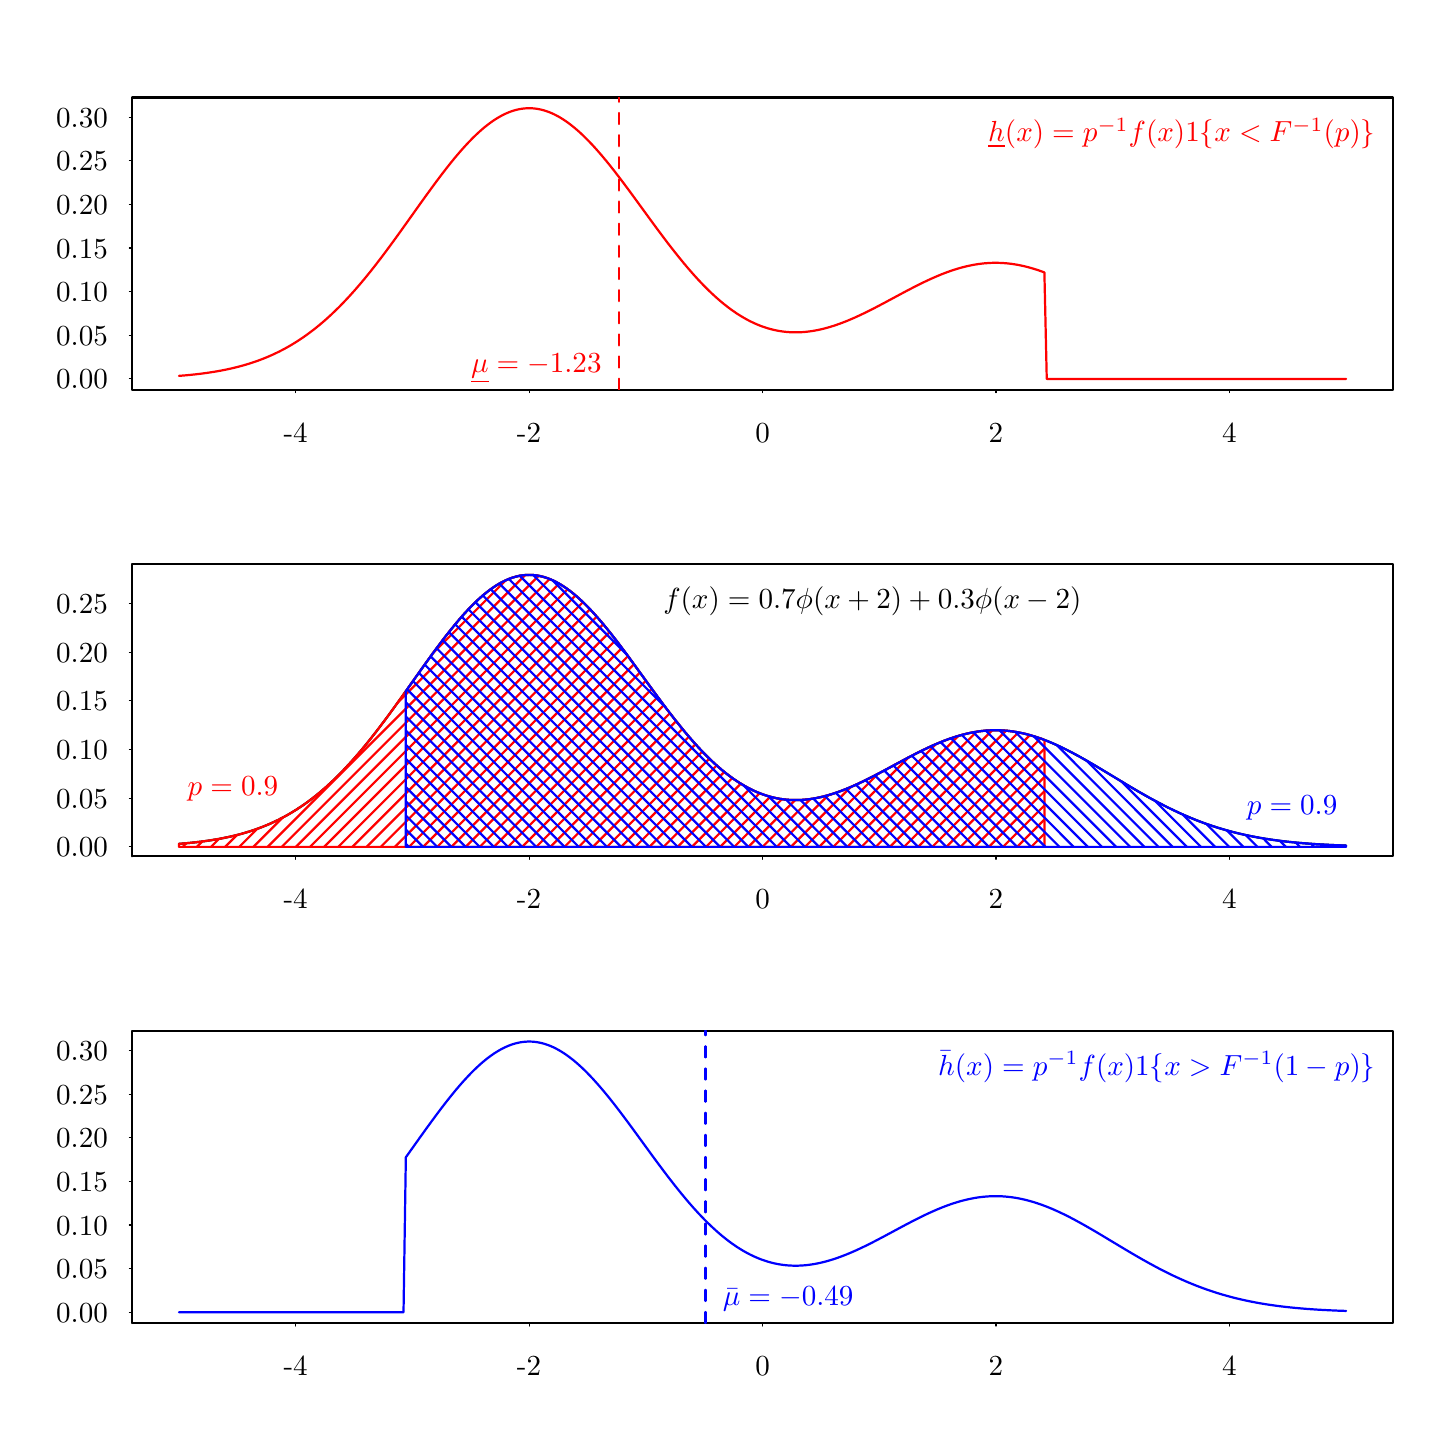
\begin{tikzpicture}[x=1pt,y=1pt]
\definecolor{fillColor}{RGB}{255,255,255}
\path[use as bounding box,fill=fillColor,fill opacity=0.00] (0,0) rectangle (505.89,505.89);
\begin{scope}
\path[clip] ( 37.80,375.06) rectangle (493.29,480.69);
\definecolor{drawColor}{RGB}{255,0,0}

\path[draw=drawColor,line width= 0.8pt,line join=round,line cap=round] ( 54.67,380.06) --
	( 55.52,380.13) --
	( 56.36,380.20) --
	( 57.21,380.27) --
	( 58.05,380.35) --
	( 58.90,380.43) --
	( 59.74,380.52) --
	( 60.59,380.61) --
	( 61.43,380.71) --
	( 62.28,380.81) --
	( 63.12,380.91) --
	( 63.97,381.03) --
	( 64.81,381.14) --
	( 65.66,381.27) --
	( 66.50,381.40) --
	( 67.35,381.53) --
	( 68.19,381.67) --
	( 69.04,381.82) --
	( 69.88,381.98) --
	( 70.73,382.14) --
	( 71.57,382.31) --
	( 72.42,382.49) --
	( 73.26,382.67) --
	( 74.11,382.87) --
	( 74.95,383.07) --
	( 75.80,383.28) --
	( 76.64,383.50) --
	( 77.49,383.73) --
	( 78.34,383.97) --
	( 79.18,384.22) --
	( 80.03,384.48) --
	( 80.87,384.75) --
	( 81.72,385.03) --
	( 82.56,385.32) --
	( 83.41,385.62) --
	( 84.25,385.94) --
	( 85.10,386.27) --
	( 85.94,386.60) --
	( 86.79,386.96) --
	( 87.63,387.32) --
	( 88.48,387.70) --
	( 89.32,388.09) --
	( 90.17,388.50) --
	( 91.01,388.91) --
	( 91.86,389.35) --
	( 92.70,389.79) --
	( 93.55,390.26) --
	( 94.39,390.73) --
	( 95.24,391.23) --
	( 96.08,391.74) --
	( 96.93,392.26) --
	( 97.77,392.80) --
	( 98.62,393.36) --
	( 99.47,393.93) --
	(100.31,394.52) --
	(101.16,395.12) --
	(102.00,395.75) --
	(102.85,396.39) --
	(103.69,397.04) --
	(104.54,397.72) --
	(105.38,398.41) --
	(106.23,399.12) --
	(107.07,399.84) --
	(107.92,400.59) --
	(108.76,401.35) --
	(109.61,402.13) --
	(110.45,402.93) --
	(111.30,403.74) --
	(112.14,404.57) --
	(112.99,405.42) --
	(113.83,406.28) --
	(114.68,407.17) --
	(115.52,408.07) --
	(116.37,408.98) --
	(117.21,409.92) --
	(118.06,410.86) --
	(118.90,411.83) --
	(119.75,412.81) --
	(120.59,413.80) --
	(121.44,414.82) --
	(122.29,415.84) --
	(123.13,416.88) --
	(123.98,417.93) --
	(124.82,419.00) --
	(125.67,420.08) --
	(126.51,421.17) --
	(127.36,422.27) --
	(128.20,423.38) --
	(129.05,424.50) --
	(129.89,425.64) --
	(130.74,426.78) --
	(131.58,427.93) --
	(132.43,429.09) --
	(133.27,430.25) --
	(134.12,431.42) --
	(134.96,432.60) --
	(135.81,433.78) --
	(136.65,434.96) --
	(137.50,436.15) --
	(138.34,437.34) --
	(139.19,438.52) --
	(140.03,439.71) --
	(140.88,440.90) --
	(141.72,442.09) --
	(142.57,443.27) --
	(143.41,444.45) --
	(144.26,445.62) --
	(145.11,446.78) --
	(145.95,447.94) --
	(146.80,449.09) --
	(147.64,450.24) --
	(148.49,451.37) --
	(149.33,452.49) --
	(150.18,453.59) --
	(151.02,454.68) --
	(151.87,455.76) --
	(152.71,456.82) --
	(153.56,457.87) --
	(154.40,458.90) --
	(155.25,459.90) --
	(156.09,460.89) --
	(156.94,461.86) --
	(157.78,462.80) --
	(158.63,463.72) --
	(159.47,464.62) --
	(160.32,465.49) --
	(161.16,466.34) --
	(162.01,467.15) --
	(162.85,467.94) --
	(163.70,468.71) --
	(164.54,469.44) --
	(165.39,470.14) --
	(166.24,470.81) --
	(167.08,471.44) --
	(167.93,472.05) --
	(168.77,472.62) --
	(169.62,473.15) --
	(170.46,473.65) --
	(171.31,474.12) --
	(172.15,474.55) --
	(173.00,474.94) --
	(173.84,475.30) --
	(174.69,475.62) --
	(175.53,475.90) --
	(176.38,476.14) --
	(177.22,476.34) --
	(178.07,476.51) --
	(178.91,476.63) --
	(179.76,476.72) --
	(180.60,476.77) --
	(181.45,476.78) --
	(182.29,476.75) --
	(183.14,476.68) --
	(183.98,476.57) --
	(184.83,476.42) --
	(185.67,476.24) --
	(186.52,476.01) --
	(187.36,475.75) --
	(188.21,475.45) --
	(189.06,475.11) --
	(189.90,474.74) --
	(190.75,474.32) --
	(191.59,473.88) --
	(192.44,473.39) --
	(193.28,472.87) --
	(194.13,472.32) --
	(194.97,471.73) --
	(195.82,471.11) --
	(196.66,470.46) --
	(197.51,469.78) --
	(198.35,469.06) --
	(199.20,468.32) --
	(200.04,467.55) --
	(200.89,466.75) --
	(201.73,465.92) --
	(202.58,465.06) --
	(203.42,464.18) --
	(204.27,463.28) --
	(205.11,462.35) --
	(205.96,461.40) --
	(206.80,460.43) --
	(207.65,459.44) --
	(208.49,458.43) --
	(209.34,457.41) --
	(210.19,456.36) --
	(211.03,455.30) --
	(211.88,454.23) --
	(212.72,453.14) --
	(213.57,452.04) --
	(214.41,450.93) --
	(215.26,449.81) --
	(216.10,448.68) --
	(216.95,447.54) --
	(217.79,446.40) --
	(218.64,445.24) --
	(219.48,444.09) --
	(220.33,442.93) --
	(221.17,441.77) --
	(222.02,440.61) --
	(222.86,439.45) --
	(223.71,438.29) --
	(224.55,437.13) --
	(225.40,435.97) --
	(226.24,434.82) --
	(227.09,433.67) --
	(227.93,432.53) --
	(228.78,431.40) --
	(229.62,430.27) --
	(230.47,429.15) --
	(231.31,428.04) --
	(232.16,426.94) --
	(233.01,425.86) --
	(233.85,424.78) --
	(234.70,423.72) --
	(235.54,422.67) --
	(236.39,421.63) --
	(237.23,420.61) --
	(238.08,419.60) --
	(238.92,418.61) --
	(239.77,417.64) --
	(240.61,416.68) --
	(241.46,415.74) --
	(242.30,414.82) --
	(243.15,413.92) --
	(243.99,413.04) --
	(244.84,412.18) --
	(245.68,411.33) --
	(246.53,410.51) --
	(247.37,409.71) --
	(248.22,408.93) --
	(249.06,408.17) --
	(249.91,407.43) --
	(250.75,406.71) --
	(251.60,406.02) --
	(252.44,405.35) --
	(253.29,404.70) --
	(254.13,404.07) --
	(254.98,403.47) --
	(255.83,402.89) --
	(256.67,402.33) --
	(257.52,401.80) --
	(258.36,401.29) --
	(259.21,400.80) --
	(260.05,400.33) --
	(260.90,399.89) --
	(261.74,399.48) --
	(262.59,399.08) --
	(263.43,398.71) --
	(264.28,398.36) --
	(265.12,398.03) --
	(265.97,397.73) --
	(266.81,397.45) --
	(267.66,397.19) --
	(268.50,396.96) --
	(269.35,396.74) --
	(270.19,396.55) --
	(271.04,396.38) --
	(271.88,396.24) --
	(272.73,396.11) --
	(273.57,396.01) --
	(274.42,395.92) --
	(275.26,395.86) --
	(276.11,395.82) --
	(276.96,395.79) --
	(277.80,395.79) --
	(278.65,395.81) --
	(279.49,395.84) --
	(280.34,395.90) --
	(281.18,395.97) --
	(282.03,396.07) --
	(282.87,396.18) --
	(283.72,396.30) --
	(284.56,396.45) --
	(285.41,396.61) --
	(286.25,396.79) --
	(287.10,396.98) --
	(287.94,397.19) --
	(288.79,397.42) --
	(289.63,397.66) --
	(290.48,397.92) --
	(291.32,398.18) --
	(292.17,398.47) --
	(293.01,398.76) --
	(293.86,399.07) --
	(294.70,399.39) --
	(295.55,399.72) --
	(296.39,400.06) --
	(297.24,400.42) --
	(298.08,400.78) --
	(298.93,401.15) --
	(299.78,401.54) --
	(300.62,401.93) --
	(301.47,402.33) --
	(302.31,402.73) --
	(303.16,403.15) --
	(304.00,403.57) --
	(304.85,403.99) --
	(305.69,404.42) --
	(306.54,404.86) --
	(307.38,405.30) --
	(308.23,405.75) --
	(309.07,406.19) --
	(309.92,406.64) --
	(310.76,407.10) --
	(311.61,407.55) --
	(312.45,408.00) --
	(313.30,408.46) --
	(314.14,408.91) --
	(314.99,409.37) --
	(315.83,409.82) --
	(316.68,410.27) --
	(317.52,410.72) --
	(318.37,411.16) --
	(319.21,411.60) --
	(320.06,412.04) --
	(320.90,412.47) --
	(321.75,412.90) --
	(322.60,413.32) --
	(323.44,413.73) --
	(324.29,414.14) --
	(325.13,414.54) --
	(325.98,414.93) --
	(326.82,415.31) --
	(327.67,415.68) --
	(328.51,416.05) --
	(329.36,416.40) --
	(330.20,416.75) --
	(331.05,417.08) --
	(331.89,417.40) --
	(332.74,417.71) --
	(333.58,418.01) --
	(334.43,418.29) --
	(335.27,418.56) --
	(336.12,418.82) --
	(336.96,419.07) --
	(337.81,419.30) --
	(338.65,419.51) --
	(339.50,419.71) --
	(340.34,419.90) --
	(341.19,420.07) --
	(342.03,420.23) --
	(342.88,420.37) --
	(343.73,420.50) --
	(344.57,420.60) --
	(345.42,420.70) --
	(346.26,420.77) --
	(347.11,420.83) --
	(347.95,420.88) --
	(348.80,420.91) --
	(349.64,420.92) --
	(350.49,420.91) --
	(351.33,420.89) --
	(352.18,420.85) --
	(353.02,420.79) --
	(353.87,420.72) --
	(354.71,420.63) --
	(355.56,420.53) --
	(356.40,420.40) --
	(357.25,420.27) --
	(358.09,420.11) --
	(358.94,419.94) --
	(359.78,419.76) --
	(360.63,419.56) --
	(361.47,419.34) --
	(362.32,419.11) --
	(363.16,418.87) --
	(364.01,418.61) --
	(364.85,418.34) --
	(365.70,418.05) --
	(366.55,417.75) --
	(367.39,417.43) --
	(368.24,378.97) --
	(369.08,378.97) --
	(369.93,378.97) --
	(370.77,378.97) --
	(371.62,378.97) --
	(372.46,378.97) --
	(373.31,378.97) --
	(374.15,378.97) --
	(375.00,378.97) --
	(375.84,378.97) --
	(376.69,378.97) --
	(377.53,378.97) --
	(378.38,378.97) --
	(379.22,378.97) --
	(380.07,378.97) --
	(380.91,378.97) --
	(381.76,378.97) --
	(382.60,378.97) --
	(383.45,378.97) --
	(384.29,378.97) --
	(385.14,378.97) --
	(385.98,378.97) --
	(386.83,378.97) --
	(387.68,378.97) --
	(388.52,378.97) --
	(389.37,378.97) --
	(390.21,378.97) --
	(391.06,378.97) --
	(391.90,378.97) --
	(392.75,378.97) --
	(393.59,378.97) --
	(394.44,378.97) --
	(395.28,378.97) --
	(396.13,378.97) --
	(396.97,378.97) --
	(397.82,378.97) --
	(398.66,378.97) --
	(399.51,378.97) --
	(400.35,378.97) --
	(401.20,378.97) --
	(402.04,378.97) --
	(402.89,378.97) --
	(403.73,378.97) --
	(404.58,378.97) --
	(405.42,378.97) --
	(406.27,378.97) --
	(407.11,378.97) --
	(407.96,378.97) --
	(408.80,378.97) --
	(409.65,378.97) --
	(410.50,378.97) --
	(411.34,378.97) --
	(412.19,378.97) --
	(413.03,378.97) --
	(413.88,378.97) --
	(414.72,378.97) --
	(415.57,378.97) --
	(416.41,378.97) --
	(417.26,378.97) --
	(418.10,378.97) --
	(418.95,378.97) --
	(419.79,378.97) --
	(420.64,378.97) --
	(421.48,378.97) --
	(422.33,378.97) --
	(423.17,378.97) --
	(424.02,378.97) --
	(424.86,378.97) --
	(425.71,378.97) --
	(426.55,378.97) --
	(427.40,378.97) --
	(428.24,378.97) --
	(429.09,378.97) --
	(429.93,378.97) --
	(430.78,378.97) --
	(431.62,378.97) --
	(432.47,378.97) --
	(433.32,378.97) --
	(434.16,378.97) --
	(435.01,378.97) --
	(435.85,378.97) --
	(436.70,378.97) --
	(437.54,378.97) --
	(438.39,378.97) --
	(439.23,378.97) --
	(440.08,378.97) --
	(440.92,378.97) --
	(441.77,378.97) --
	(442.61,378.97) --
	(443.46,378.97) --
	(444.30,378.97) --
	(445.15,378.97) --
	(445.99,378.97) --
	(446.84,378.97) --
	(447.68,378.97) --
	(448.53,378.97) --
	(449.37,378.97) --
	(450.22,378.97) --
	(451.06,378.97) --
	(451.91,378.97) --
	(452.75,378.97) --
	(453.60,378.97) --
	(454.45,378.97) --
	(455.29,378.97) --
	(456.14,378.97) --
	(456.98,378.97) --
	(457.83,378.97) --
	(458.67,378.97) --
	(459.52,378.97) --
	(460.36,378.97) --
	(461.21,378.97) --
	(462.05,378.97) --
	(462.90,378.97) --
	(463.74,378.97) --
	(464.59,378.97) --
	(465.43,378.97) --
	(466.28,378.97) --
	(467.12,378.97) --
	(467.97,378.97) --
	(468.81,378.97) --
	(469.66,378.97) --
	(470.50,378.97) --
	(471.35,378.97) --
	(472.19,378.97) --
	(473.04,378.97) --
	(473.88,378.97) --
	(474.73,378.97) --
	(475.57,378.97) --
	(476.42,378.97);
\end{scope}
\begin{scope}
\path[clip] (  0.00,  0.00) rectangle (505.89,505.89);
\definecolor{drawColor}{RGB}{0,0,0}

\path[draw=drawColor,line width= 0.4pt,line join=round,line cap=round] ( 96.84,375.06) -- (434.25,375.06);

\path[draw=drawColor,line width= 0.4pt,line join=round,line cap=round] ( 96.84,375.06) -- ( 96.84,374.00);

\path[draw=drawColor,line width= 0.4pt,line join=round,line cap=round] (181.19,375.06) -- (181.19,374.00);

\path[draw=drawColor,line width= 0.4pt,line join=round,line cap=round] (265.54,375.06) -- (265.54,374.00);

\path[draw=drawColor,line width= 0.4pt,line join=round,line cap=round] (349.89,375.06) -- (349.89,374.00);

\path[draw=drawColor,line width= 0.4pt,line join=round,line cap=round] (434.25,375.06) -- (434.25,374.00);

\node[text=drawColor,anchor=base,inner sep=0pt, outer sep=0pt, scale=  1.05] at ( 96.84,356.16) {-4};

\node[text=drawColor,anchor=base,inner sep=0pt, outer sep=0pt, scale=  1.05] at (181.19,356.16) {-2};

\node[text=drawColor,anchor=base,inner sep=0pt, outer sep=0pt, scale=  1.05] at (265.54,356.16) {0};

\node[text=drawColor,anchor=base,inner sep=0pt, outer sep=0pt, scale=  1.05] at (349.89,356.16) {2};

\node[text=drawColor,anchor=base,inner sep=0pt, outer sep=0pt, scale=  1.05] at (434.25,356.16) {4};

\path[draw=drawColor,line width= 0.4pt,line join=round,line cap=round] ( 37.80,378.97) -- ( 37.80,473.52);

\path[draw=drawColor,line width= 0.4pt,line join=round,line cap=round] ( 37.80,378.97) -- ( 36.74,378.97);

\path[draw=drawColor,line width= 0.4pt,line join=round,line cap=round] ( 37.80,394.73) -- ( 36.74,394.73);

\path[draw=drawColor,line width= 0.4pt,line join=round,line cap=round] ( 37.80,410.49) -- ( 36.74,410.49);

\path[draw=drawColor,line width= 0.4pt,line join=round,line cap=round] ( 37.80,426.25) -- ( 36.74,426.25);

\path[draw=drawColor,line width= 0.4pt,line join=round,line cap=round] ( 37.80,442.01) -- ( 36.74,442.01);

\path[draw=drawColor,line width= 0.4pt,line join=round,line cap=round] ( 37.80,457.76) -- ( 36.74,457.76);

\path[draw=drawColor,line width= 0.4pt,line join=round,line cap=round] ( 37.80,473.52) -- ( 36.74,473.52);

\node[text=drawColor,anchor=base east,inner sep=0pt, outer sep=0pt, scale=  1.05] at ( 28.98,375.36) {0.00};

\node[text=drawColor,anchor=base east,inner sep=0pt, outer sep=0pt, scale=  1.05] at ( 28.98,391.11) {0.05};

\node[text=drawColor,anchor=base east,inner sep=0pt, outer sep=0pt, scale=  1.05] at ( 28.98,406.87) {0.10};

\node[text=drawColor,anchor=base east,inner sep=0pt, outer sep=0pt, scale=  1.05] at ( 28.98,422.63) {0.15};

\node[text=drawColor,anchor=base east,inner sep=0pt, outer sep=0pt, scale=  1.05] at ( 28.98,438.39) {0.20};

\node[text=drawColor,anchor=base east,inner sep=0pt, outer sep=0pt, scale=  1.05] at ( 28.98,454.15) {0.25};

\node[text=drawColor,anchor=base east,inner sep=0pt, outer sep=0pt, scale=  1.05] at ( 28.98,469.91) {0.30};

\path[draw=drawColor,line width= 0.8pt,line join=round,line cap=round] ( 37.80,375.06) --
	(493.29,375.06) --
	(493.29,480.69) --
	( 37.80,480.69) --
	( 37.80,375.06);
\end{scope}
\begin{scope}
\path[clip] ( 37.80,375.06) rectangle (493.29,480.69);
\definecolor{drawColor}{RGB}{255,0,0}

\node[text=drawColor,anchor=base east,inner sep=0pt, outer sep=0pt, scale=  1.05] at (486.99,464.59) {$\underline{h}(x) = p^{-1}f(x) 1\{x < F^{-1}(p)\}$};

\path[draw=drawColor,line width= 0.8pt,dash pattern=on 4pt off 4pt ,line join=round,line cap=round] (213.67,375.06) -- (213.67,480.69);

\node[text=drawColor,anchor=base east,inner sep=0pt, outer sep=0pt, scale=  1.05] at (207.37,381.45) {$\underline{\mu} = -1.23$};
\end{scope}
\begin{scope}
\path[clip] ( 37.80,206.43) rectangle (493.29,312.06);
\definecolor{drawColor}{RGB}{0,0,0}

\path[draw=drawColor,line width= 0.8pt,line join=round,line cap=round] ( 54.67,210.97) --
	( 55.52,211.03) --
	( 56.36,211.10) --
	( 57.21,211.18) --
	( 58.05,211.26) --
	( 58.90,211.34) --
	( 59.74,211.43) --
	( 60.59,211.52) --
	( 61.43,211.62) --
	( 62.28,211.72) --
	( 63.12,211.83) --
	( 63.97,211.94) --
	( 64.81,212.06) --
	( 65.66,212.18) --
	( 66.50,212.31) --
	( 67.35,212.45) --
	( 68.19,212.59) --
	( 69.04,212.74) --
	( 69.88,212.89) --
	( 70.73,213.06) --
	( 71.57,213.23) --
	( 72.42,213.41) --
	( 73.26,213.59) --
	( 74.11,213.79) --
	( 74.95,213.99) --
	( 75.80,214.20) --
	( 76.64,214.42) --
	( 77.49,214.65) --
	( 78.34,214.90) --
	( 79.18,215.15) --
	( 80.03,215.41) --
	( 80.87,215.68) --
	( 81.72,215.96) --
	( 82.56,216.25) --
	( 83.41,216.56) --
	( 84.25,216.87) --
	( 85.10,217.20) --
	( 85.94,217.54) --
	( 86.79,217.90) --
	( 87.63,218.26) --
	( 88.48,218.64) --
	( 89.32,219.04) --
	( 90.17,219.44) --
	( 91.01,219.86) --
	( 91.86,220.30) --
	( 92.70,220.75) --
	( 93.55,221.21) --
	( 94.39,221.69) --
	( 95.24,222.19) --
	( 96.08,222.70) --
	( 96.93,223.23) --
	( 97.77,223.77) --
	( 98.62,224.33) --
	( 99.47,224.90) --
	(100.31,225.49) --
	(101.16,226.10) --
	(102.00,226.73) --
	(102.85,227.37) --
	(103.69,228.03) --
	(104.54,228.71) --
	(105.38,229.40) --
	(106.23,230.12) --
	(107.07,230.85) --
	(107.92,231.59) --
	(108.76,232.36) --
	(109.61,233.14) --
	(110.45,233.94) --
	(111.30,234.76) --
	(112.14,235.59) --
	(112.99,236.45) --
	(113.83,237.32) --
	(114.68,238.20) --
	(115.52,239.11) --
	(116.37,240.03) --
	(117.21,240.97) --
	(118.06,241.92) --
	(118.90,242.89) --
	(119.75,243.87) --
	(120.59,244.87) --
	(121.44,245.89) --
	(122.29,246.92) --
	(123.13,247.96) --
	(123.98,249.02) --
	(124.82,250.09) --
	(125.67,251.17) --
	(126.51,252.27) --
	(127.36,253.38) --
	(128.20,254.50) --
	(129.05,255.62) --
	(129.89,256.76) --
	(130.74,257.91) --
	(131.58,259.07) --
	(132.43,260.23) --
	(133.27,261.40) --
	(134.12,262.58) --
	(134.96,263.76) --
	(135.81,264.94) --
	(136.65,266.13) --
	(137.50,267.32) --
	(138.34,268.52) --
	(139.19,269.71) --
	(140.03,270.91) --
	(140.88,272.10) --
	(141.72,273.29) --
	(142.57,274.48) --
	(143.41,275.66) --
	(144.26,276.84) --
	(145.11,278.01) --
	(145.95,279.18) --
	(146.80,280.33) --
	(147.64,281.48) --
	(148.49,282.61) --
	(149.33,283.74) --
	(150.18,284.85) --
	(151.02,285.95) --
	(151.87,287.03) --
	(152.71,288.10) --
	(153.56,289.15) --
	(154.40,290.18) --
	(155.25,291.19) --
	(156.09,292.19) --
	(156.94,293.16) --
	(157.78,294.11) --
	(158.63,295.03) --
	(159.47,295.93) --
	(160.32,296.81) --
	(161.16,297.66) --
	(162.01,298.48) --
	(162.85,299.27) --
	(163.70,300.04) --
	(164.54,300.77) --
	(165.39,301.47) --
	(166.24,302.15) --
	(167.08,302.79) --
	(167.93,303.39) --
	(168.77,303.97) --
	(169.62,304.51) --
	(170.46,305.01) --
	(171.31,305.48) --
	(172.15,305.91) --
	(173.00,306.30) --
	(173.84,306.66) --
	(174.69,306.98) --
	(175.53,307.26) --
	(176.38,307.50) --
	(177.22,307.71) --
	(178.07,307.88) --
	(178.91,308.00) --
	(179.76,308.09) --
	(180.60,308.14) --
	(181.45,308.15) --
	(182.29,308.12) --
	(183.14,308.05) --
	(183.98,307.94) --
	(184.83,307.79) --
	(185.67,307.60) --
	(186.52,307.38) --
	(187.36,307.11) --
	(188.21,306.81) --
	(189.06,306.47) --
	(189.90,306.10) --
	(190.75,305.68) --
	(191.59,305.23) --
	(192.44,304.75) --
	(193.28,304.22) --
	(194.13,303.67) --
	(194.97,303.08) --
	(195.82,302.46) --
	(196.66,301.80) --
	(197.51,301.12) --
	(198.35,300.40) --
	(199.20,299.65) --
	(200.04,298.87) --
	(200.89,298.07) --
	(201.73,297.24) --
	(202.58,296.38) --
	(203.42,295.49) --
	(204.27,294.59) --
	(205.11,293.65) --
	(205.96,292.70) --
	(206.80,291.73) --
	(207.65,290.73) --
	(208.49,289.72) --
	(209.34,288.68) --
	(210.19,287.63) --
	(211.03,286.57) --
	(211.88,285.49) --
	(212.72,284.40) --
	(213.57,283.29) --
	(214.41,282.18) --
	(215.26,281.05) --
	(216.10,279.91) --
	(216.95,278.77) --
	(217.79,277.62) --
	(218.64,276.46) --
	(219.48,275.30) --
	(220.33,274.14) --
	(221.17,272.97) --
	(222.02,271.81) --
	(222.86,270.64) --
	(223.71,269.47) --
	(224.55,268.31) --
	(225.40,267.15) --
	(226.24,265.99) --
	(227.09,264.84) --
	(227.93,263.69) --
	(228.78,262.55) --
	(229.62,261.42) --
	(230.47,260.29) --
	(231.31,259.18) --
	(232.16,258.08) --
	(233.01,256.98) --
	(233.85,255.90) --
	(234.70,254.83) --
	(235.54,253.78) --
	(236.39,252.74) --
	(237.23,251.71) --
	(238.08,250.70) --
	(238.92,249.71) --
	(239.77,248.73) --
	(240.61,247.77) --
	(241.46,246.82) --
	(242.30,245.90) --
	(243.15,244.99) --
	(243.99,244.10) --
	(244.84,243.24) --
	(245.68,242.39) --
	(246.53,241.56) --
	(247.37,240.76) --
	(248.22,239.97) --
	(249.06,239.21) --
	(249.91,238.47) --
	(250.75,237.75) --
	(251.60,237.05) --
	(252.44,236.38) --
	(253.29,235.73) --
	(254.13,235.10) --
	(254.98,234.49) --
	(255.83,233.91) --
	(256.67,233.35) --
	(257.52,232.81) --
	(258.36,232.30) --
	(259.21,231.81) --
	(260.05,231.34) --
	(260.90,230.90) --
	(261.74,230.48) --
	(262.59,230.08) --
	(263.43,229.70) --
	(264.28,229.35) --
	(265.12,229.03) --
	(265.97,228.72) --
	(266.81,228.44) --
	(267.66,228.18) --
	(268.50,227.94) --
	(269.35,227.73) --
	(270.19,227.54) --
	(271.04,227.37) --
	(271.88,227.22) --
	(272.73,227.09) --
	(273.57,226.99) --
	(274.42,226.90) --
	(275.26,226.84) --
	(276.11,226.80) --
	(276.96,226.78) --
	(277.80,226.77) --
	(278.65,226.79) --
	(279.49,226.83) --
	(280.34,226.88) --
	(281.18,226.96) --
	(282.03,227.05) --
	(282.87,227.16) --
	(283.72,227.29) --
	(284.56,227.44) --
	(285.41,227.60) --
	(286.25,227.78) --
	(287.10,227.97) --
	(287.94,228.18) --
	(288.79,228.41) --
	(289.63,228.65) --
	(290.48,228.91) --
	(291.32,229.18) --
	(292.17,229.46) --
	(293.01,229.76) --
	(293.86,230.07) --
	(294.70,230.39) --
	(295.55,230.72) --
	(296.39,231.07) --
	(297.24,231.42) --
	(298.08,231.79) --
	(298.93,232.16) --
	(299.78,232.55) --
	(300.62,232.94) --
	(301.47,233.34) --
	(302.31,233.75) --
	(303.16,234.16) --
	(304.00,234.59) --
	(304.85,235.01) --
	(305.69,235.45) --
	(306.54,235.89) --
	(307.38,236.33) --
	(308.23,236.78) --
	(309.07,237.23) --
	(309.92,237.68) --
	(310.76,238.13) --
	(311.61,238.59) --
	(312.45,239.05) --
	(313.30,239.50) --
	(314.14,239.96) --
	(314.99,240.41) --
	(315.83,240.87) --
	(316.68,241.32) --
	(317.52,241.77) --
	(318.37,242.22) --
	(319.21,242.66) --
	(320.06,243.10) --
	(320.90,243.53) --
	(321.75,243.96) --
	(322.60,244.38) --
	(323.44,244.80) --
	(324.29,245.21) --
	(325.13,245.61) --
	(325.98,246.00) --
	(326.82,246.39) --
	(327.67,246.76) --
	(328.51,247.13) --
	(329.36,247.48) --
	(330.20,247.83) --
	(331.05,248.16) --
	(331.89,248.49) --
	(332.74,248.80) --
	(333.58,249.09) --
	(334.43,249.38) --
	(335.27,249.65) --
	(336.12,249.91) --
	(336.96,250.16) --
	(337.81,250.39) --
	(338.65,250.61) --
	(339.50,250.81) --
	(340.34,251.00) --
	(341.19,251.17) --
	(342.03,251.33) --
	(342.88,251.47) --
	(343.73,251.60) --
	(344.57,251.71) --
	(345.42,251.80) --
	(346.26,251.88) --
	(347.11,251.94) --
	(347.95,251.98) --
	(348.80,252.01) --
	(349.64,252.02) --
	(350.49,252.01) --
	(351.33,251.99) --
	(352.18,251.95) --
	(353.02,251.89) --
	(353.87,251.82) --
	(354.71,251.73) --
	(355.56,251.63) --
	(356.40,251.51) --
	(357.25,251.37) --
	(358.09,251.21) --
	(358.94,251.04) --
	(359.78,250.86) --
	(360.63,250.66) --
	(361.47,250.44) --
	(362.32,250.21) --
	(363.16,249.96) --
	(364.01,249.70) --
	(364.85,249.43) --
	(365.70,249.14) --
	(366.55,248.84) --
	(367.39,248.52) --
	(368.24,248.19) --
	(369.08,247.85) --
	(369.93,247.50) --
	(370.77,247.13) --
	(371.62,246.76) --
	(372.46,246.37) --
	(373.31,245.98) --
	(374.15,245.57) --
	(375.00,245.15) --
	(375.84,244.73) --
	(376.69,244.29) --
	(377.53,243.85) --
	(378.38,243.40) --
	(379.22,242.94) --
	(380.07,242.48) --
	(380.91,242.01) --
	(381.76,241.53) --
	(382.60,241.05) --
	(383.45,240.56) --
	(384.29,240.07) --
	(385.14,239.58) --
	(385.98,239.08) --
	(386.83,238.57) --
	(387.68,238.07) --
	(388.52,237.56) --
	(389.37,237.05) --
	(390.21,236.54) --
	(391.06,236.03) --
	(391.90,235.52) --
	(392.75,235.01) --
	(393.59,234.50) --
	(394.44,233.98) --
	(395.28,233.48) --
	(396.13,232.97) --
	(396.97,232.46) --
	(397.82,231.96) --
	(398.66,231.46) --
	(399.51,230.96) --
	(400.35,230.46) --
	(401.20,229.97) --
	(402.04,229.48) --
	(402.89,229.00) --
	(403.73,228.52) --
	(404.58,228.04) --
	(405.42,227.57) --
	(406.27,227.11) --
	(407.11,226.65) --
	(407.96,226.20) --
	(408.80,225.75) --
	(409.65,225.31) --
	(410.50,224.87) --
	(411.34,224.45) --
	(412.19,224.02) --
	(413.03,223.61) --
	(413.88,223.20) --
	(414.72,222.80) --
	(415.57,222.40) --
	(416.41,222.02) --
	(417.26,221.64) --
	(418.10,221.26) --
	(418.95,220.90) --
	(419.79,220.54) --
	(420.64,220.19) --
	(421.48,219.85) --
	(422.33,219.51) --
	(423.17,219.18) --
	(424.02,218.86) --
	(424.86,218.55) --
	(425.71,218.24) --
	(426.55,217.95) --
	(427.40,217.66) --
	(428.24,217.37) --
	(429.09,217.10) --
	(429.93,216.83) --
	(430.78,216.57) --
	(431.62,216.32) --
	(432.47,216.07) --
	(433.32,215.83) --
	(434.16,215.60) --
	(435.01,215.37) --
	(435.85,215.15) --
	(436.70,214.94) --
	(437.54,214.73) --
	(438.39,214.53) --
	(439.23,214.34) --
	(440.08,214.16) --
	(440.92,213.98) --
	(441.77,213.80) --
	(442.61,213.63) --
	(443.46,213.47) --
	(444.30,213.31) --
	(445.15,213.16) --
	(445.99,213.02) --
	(446.84,212.87) --
	(447.68,212.74) --
	(448.53,212.61) --
	(449.37,212.48) --
	(450.22,212.36) --
	(451.06,212.25) --
	(451.91,212.13) --
	(452.75,212.03) --
	(453.60,211.92) --
	(454.45,211.82) --
	(455.29,211.73) --
	(456.14,211.64) --
	(456.98,211.55) --
	(457.83,211.47) --
	(458.67,211.39) --
	(459.52,211.31) --
	(460.36,211.24) --
	(461.21,211.17) --
	(462.05,211.10) --
	(462.90,211.04) --
	(463.74,210.98) --
	(464.59,210.92) --
	(465.43,210.86) --
	(466.28,210.81) --
	(467.12,210.76) --
	(467.97,210.71) --
	(468.81,210.67) --
	(469.66,210.62) --
	(470.50,210.58) --
	(471.35,210.54) --
	(472.19,210.50) --
	(473.04,210.47) --
	(473.88,210.43) --
	(474.73,210.40) --
	(475.57,210.37) --
	(476.42,210.34);
\end{scope}
\begin{scope}
\path[clip] (  0.00,  0.00) rectangle (505.89,505.89);
\definecolor{drawColor}{RGB}{0,0,0}

\path[draw=drawColor,line width= 0.4pt,line join=round,line cap=round] ( 96.84,206.43) -- (434.25,206.43);

\path[draw=drawColor,line width= 0.4pt,line join=round,line cap=round] ( 96.84,206.43) -- ( 96.84,205.37);

\path[draw=drawColor,line width= 0.4pt,line join=round,line cap=round] (181.19,206.43) -- (181.19,205.37);

\path[draw=drawColor,line width= 0.4pt,line join=round,line cap=round] (265.54,206.43) -- (265.54,205.37);

\path[draw=drawColor,line width= 0.4pt,line join=round,line cap=round] (349.89,206.43) -- (349.89,205.37);

\path[draw=drawColor,line width= 0.4pt,line join=round,line cap=round] (434.25,206.43) -- (434.25,205.37);

\node[text=drawColor,anchor=base,inner sep=0pt, outer sep=0pt, scale=  1.05] at ( 96.84,187.53) {-4};

\node[text=drawColor,anchor=base,inner sep=0pt, outer sep=0pt, scale=  1.05] at (181.19,187.53) {-2};

\node[text=drawColor,anchor=base,inner sep=0pt, outer sep=0pt, scale=  1.05] at (265.54,187.53) {0};

\node[text=drawColor,anchor=base,inner sep=0pt, outer sep=0pt, scale=  1.05] at (349.89,187.53) {2};

\node[text=drawColor,anchor=base,inner sep=0pt, outer sep=0pt, scale=  1.05] at (434.25,187.53) {4};

\path[draw=drawColor,line width= 0.4pt,line join=round,line cap=round] ( 37.80,209.87) -- ( 37.80,297.84);

\path[draw=drawColor,line width= 0.4pt,line join=round,line cap=round] ( 37.80,209.87) -- ( 36.74,209.87);

\path[draw=drawColor,line width= 0.4pt,line join=round,line cap=round] ( 37.80,227.47) -- ( 36.74,227.47);

\path[draw=drawColor,line width= 0.4pt,line join=round,line cap=round] ( 37.80,245.06) -- ( 36.74,245.06);

\path[draw=drawColor,line width= 0.4pt,line join=round,line cap=round] ( 37.80,262.65) -- ( 36.74,262.65);

\path[draw=drawColor,line width= 0.4pt,line join=round,line cap=round] ( 37.80,280.25) -- ( 36.74,280.25);

\path[draw=drawColor,line width= 0.4pt,line join=round,line cap=round] ( 37.80,297.84) -- ( 36.74,297.84);

\node[text=drawColor,anchor=base east,inner sep=0pt, outer sep=0pt, scale=  1.05] at ( 28.98,206.26) {0.00};

\node[text=drawColor,anchor=base east,inner sep=0pt, outer sep=0pt, scale=  1.05] at ( 28.98,223.85) {0.05};

\node[text=drawColor,anchor=base east,inner sep=0pt, outer sep=0pt, scale=  1.05] at ( 28.98,241.44) {0.10};

\node[text=drawColor,anchor=base east,inner sep=0pt, outer sep=0pt, scale=  1.05] at ( 28.98,259.04) {0.15};

\node[text=drawColor,anchor=base east,inner sep=0pt, outer sep=0pt, scale=  1.05] at ( 28.98,276.63) {0.20};

\node[text=drawColor,anchor=base east,inner sep=0pt, outer sep=0pt, scale=  1.05] at ( 28.98,294.22) {0.25};

\path[draw=drawColor,line width= 0.8pt,line join=round,line cap=round] ( 37.80,206.43) --
	(493.29,206.43) --
	(493.29,312.06) --
	( 37.80,312.06) --
	( 37.80,206.43);
\end{scope}
\begin{scope}
\path[clip] ( 37.80,206.43) rectangle (493.29,312.06);
\definecolor{drawColor}{RGB}{255,0,0}

\path[draw=drawColor,line width= 0.8pt,line join=round,line cap=round] ( 56.02,209.87) -- ( 57.34,211.19);

\path[draw=drawColor,line width= 0.8pt,line join=round,line cap=round] ( 61.13,209.87) -- ( 63.08,211.82);

\path[draw=drawColor,line width= 0.8pt,line join=round,line cap=round] ( 66.24,209.87) -- ( 69.12,212.75);

\path[draw=drawColor,line width= 0.8pt,line join=round,line cap=round] ( 71.36,209.87) -- ( 75.64,214.16);

\path[draw=drawColor,line width= 0.8pt,line join=round,line cap=round] ( 76.47,209.87) -- ( 83.00,216.41);

\path[draw=drawColor,line width= 0.8pt,line join=round,line cap=round] (146.45,279.86) -- (172.80,306.21);

\path[draw=drawColor,line width= 0.8pt,line join=round,line cap=round] ( 81.58,209.87) -- ( 92.16,220.46);

\path[draw=drawColor,line width= 0.8pt,line join=round,line cap=round] (133.71,262.01) -- (179.79,308.09);

\path[draw=drawColor,line width= 0.8pt,line join=round,line cap=round] ( 86.69,209.87) -- (184.64,307.82);

\path[draw=drawColor,line width= 0.8pt,line join=round,line cap=round] ( 91.80,209.87) -- (188.58,306.66);

\path[draw=drawColor,line width= 0.8pt,line join=round,line cap=round] ( 96.91,209.87) -- (192.02,304.99);

\path[draw=drawColor,line width= 0.8pt,line join=round,line cap=round] (102.02,209.87) -- (195.12,302.97);

\path[draw=drawColor,line width= 0.8pt,line join=round,line cap=round] (107.13,209.87) -- (197.97,300.72);

\path[draw=drawColor,line width= 0.8pt,line join=round,line cap=round] (112.24,209.87) -- (200.65,298.29);

\path[draw=drawColor,line width= 0.8pt,line join=round,line cap=round] (117.35,209.87) -- (203.20,295.73);

\path[draw=drawColor,line width= 0.8pt,line join=round,line cap=round] (122.46,209.87) -- (205.64,293.06);

\path[draw=drawColor,line width= 0.8pt,line join=round,line cap=round] (127.57,209.87) -- (208.00,290.31);

\path[draw=drawColor,line width= 0.8pt,line join=round,line cap=round] (132.68,209.87) -- (210.30,287.49);

\path[draw=drawColor,line width= 0.8pt,line join=round,line cap=round] (137.79,209.87) -- (212.54,284.63);

\path[draw=drawColor,line width= 0.8pt,line join=round,line cap=round] (142.90,209.87) -- (214.75,281.72);

\path[draw=drawColor,line width= 0.8pt,line join=round,line cap=round] (148.01,209.87) -- (216.93,278.79);

\path[draw=drawColor,line width= 0.8pt,line join=round,line cap=round] (153.12,209.87) -- (219.09,275.84);

\path[draw=drawColor,line width= 0.8pt,line join=round,line cap=round] (158.23,209.87) -- (221.24,272.88);

\path[draw=drawColor,line width= 0.8pt,line join=round,line cap=round] (163.34,209.87) -- (223.39,269.92);

\path[draw=drawColor,line width= 0.8pt,line join=round,line cap=round] (168.45,209.87) -- (225.54,266.96);

\path[draw=drawColor,line width= 0.8pt,line join=round,line cap=round] (173.56,209.87) -- (227.70,264.01);

\path[draw=drawColor,line width= 0.8pt,line join=round,line cap=round] (178.67,209.87) -- (229.88,261.08);

\path[draw=drawColor,line width= 0.8pt,line join=round,line cap=round] (183.78,209.87) -- (232.08,258.18);

\path[draw=drawColor,line width= 0.8pt,line join=round,line cap=round] (188.89,209.87) -- (234.32,255.31);

\path[draw=drawColor,line width= 0.8pt,line join=round,line cap=round] (194.00,209.87) -- (236.60,252.47);

\path[draw=drawColor,line width= 0.8pt,line join=round,line cap=round] (199.11,209.87) -- (238.93,249.69);

\path[draw=drawColor,line width= 0.8pt,line join=round,line cap=round] (204.22,209.87) -- (241.32,246.97);

\path[draw=drawColor,line width= 0.8pt,line join=round,line cap=round] (209.33,209.87) -- (243.78,244.32);

\path[draw=drawColor,line width= 0.8pt,line join=round,line cap=round] (214.44,209.87) -- (246.33,241.76);

\path[draw=drawColor,line width= 0.8pt,line join=round,line cap=round] (219.55,209.87) -- (248.97,239.29);

\path[draw=drawColor,line width= 0.8pt,line join=round,line cap=round] (224.66,209.87) -- (251.73,236.95);

\path[draw=drawColor,line width= 0.8pt,line join=round,line cap=round] (229.77,209.87) -- (254.64,234.74);

\path[draw=drawColor,line width= 0.8pt,line join=round,line cap=round] (234.88,209.87) -- (257.70,232.70);

\path[draw=drawColor,line width= 0.8pt,line join=round,line cap=round] (239.99,209.87) -- (260.98,230.86);

\path[draw=drawColor,line width= 0.8pt,line join=round,line cap=round] (245.10,209.87) -- (264.50,229.27);

\path[draw=drawColor,line width= 0.8pt,line join=round,line cap=round] (250.21,209.87) -- (268.33,227.99);

\path[draw=drawColor,line width= 0.8pt,line join=round,line cap=round] (255.32,209.87) -- (272.57,227.12);

\path[draw=drawColor,line width= 0.8pt,line join=round,line cap=round] (260.43,209.87) -- (277.34,226.77);

\path[draw=drawColor,line width= 0.8pt,line join=round,line cap=round] (265.54,209.87) -- (282.83,227.15);

\path[draw=drawColor,line width= 0.8pt,line join=round,line cap=round] (270.66,209.87) -- (289.35,228.57);

\path[draw=drawColor,line width= 0.8pt,line join=round,line cap=round] (275.77,209.87) -- (297.37,231.48);

\path[draw=drawColor,line width= 0.8pt,line join=round,line cap=round] (280.88,209.87) -- (307.28,236.27);

\path[draw=drawColor,line width= 0.8pt,line join=round,line cap=round] (285.99,209.87) -- (318.28,242.17);

\path[draw=drawColor,line width= 0.8pt,line join=round,line cap=round] (291.10,209.87) -- (328.22,247.00);

\path[draw=drawColor,line width= 0.8pt,line join=round,line cap=round] (296.21,209.87) -- (336.30,249.97);

\path[draw=drawColor,line width= 0.8pt,line join=round,line cap=round] (301.32,209.87) -- (342.92,251.48);

\path[draw=drawColor,line width= 0.8pt,line join=round,line cap=round] (306.43,209.87) -- (348.55,252.00);

\path[draw=drawColor,line width= 0.8pt,line join=round,line cap=round] (311.54,209.87) -- (353.52,251.85);

\path[draw=drawColor,line width= 0.8pt,line join=round,line cap=round] (316.65,209.87) -- (358.00,251.23);

\path[draw=drawColor,line width= 0.8pt,line join=round,line cap=round] (321.76,209.87) -- (362.14,250.26);

\path[draw=drawColor,line width= 0.8pt,line join=round,line cap=round] (326.87,209.87) -- (366.02,249.02);

\path[draw=drawColor,line width= 0.8pt,line join=round,line cap=round] (331.98,209.87) -- (367.39,245.29);

\path[draw=drawColor,line width= 0.8pt,line join=round,line cap=round] (337.09,209.87) -- (367.39,240.18);

\path[draw=drawColor,line width= 0.8pt,line join=round,line cap=round] (342.20,209.87) -- (367.39,235.07);

\path[draw=drawColor,line width= 0.8pt,line join=round,line cap=round] (347.31,209.87) -- (367.39,229.96);

\path[draw=drawColor,line width= 0.8pt,line join=round,line cap=round] (352.42,209.87) -- (367.39,224.85);

\path[draw=drawColor,line width= 0.8pt,line join=round,line cap=round] (357.53,209.87) -- (367.39,219.74);

\path[draw=drawColor,line width= 0.8pt,line join=round,line cap=round] (362.64,209.87) -- (367.39,214.62);

\path[draw=drawColor,line width= 0.8pt,line join=round,line cap=round] ( 54.67,209.87) --
	( 55.52,209.87) --
	( 56.36,209.87) --
	( 57.21,209.87) --
	( 58.05,209.87) --
	( 58.90,209.87) --
	( 59.74,209.87) --
	( 60.59,209.87) --
	( 61.43,209.87) --
	( 62.28,209.87) --
	( 63.12,209.87) --
	( 63.97,209.87) --
	( 64.81,209.87) --
	( 65.66,209.87) --
	( 66.50,209.87) --
	( 67.35,209.87) --
	( 68.19,209.87) --
	( 69.04,209.87) --
	( 69.88,209.87) --
	( 70.73,209.87) --
	( 71.57,209.87) --
	( 72.42,209.87) --
	( 73.26,209.87) --
	( 74.11,209.87) --
	( 74.95,209.87) --
	( 75.80,209.87) --
	( 76.64,209.87) --
	( 77.49,209.87) --
	( 78.34,209.87) --
	( 79.18,209.87) --
	( 80.03,209.87) --
	( 80.87,209.87) --
	( 81.72,209.87) --
	( 82.56,209.87) --
	( 83.41,209.87) --
	( 84.25,209.87) --
	( 85.10,209.87) --
	( 85.94,209.87) --
	( 86.79,209.87) --
	( 87.63,209.87) --
	( 88.48,209.87) --
	( 89.32,209.87) --
	( 90.17,209.87) --
	( 91.01,209.87) --
	( 91.86,209.87) --
	( 92.70,209.87) --
	( 93.55,209.87) --
	( 94.39,209.87) --
	( 95.24,209.87) --
	( 96.08,209.87) --
	( 96.93,209.87) --
	( 97.77,209.87) --
	( 98.62,209.87) --
	( 99.47,209.87) --
	(100.31,209.87) --
	(101.16,209.87) --
	(102.00,209.87) --
	(102.85,209.87) --
	(103.69,209.87) --
	(104.54,209.87) --
	(105.38,209.87) --
	(106.23,209.87) --
	(107.07,209.87) --
	(107.92,209.87) --
	(108.76,209.87) --
	(109.61,209.87) --
	(110.45,209.87) --
	(111.30,209.87) --
	(112.14,209.87) --
	(112.99,209.87) --
	(113.83,209.87) --
	(114.68,209.87) --
	(115.52,209.87) --
	(116.37,209.87) --
	(117.21,209.87) --
	(118.06,209.87) --
	(118.90,209.87) --
	(119.75,209.87) --
	(120.59,209.87) --
	(121.44,209.87) --
	(122.29,209.87) --
	(123.13,209.87) --
	(123.98,209.87) --
	(124.82,209.87) --
	(125.67,209.87) --
	(126.51,209.87) --
	(127.36,209.87) --
	(128.20,209.87) --
	(129.05,209.87) --
	(129.89,209.87) --
	(130.74,209.87) --
	(131.58,209.87) --
	(132.43,209.87) --
	(133.27,209.87) --
	(134.12,209.87) --
	(134.96,209.87) --
	(135.81,209.87) --
	(136.65,209.87) --
	(137.50,209.87) --
	(138.34,209.87) --
	(139.19,209.87) --
	(140.03,209.87) --
	(140.88,209.87) --
	(141.72,209.87) --
	(142.57,209.87) --
	(143.41,209.87) --
	(144.26,209.87) --
	(145.11,209.87) --
	(145.95,209.87) --
	(146.80,209.87) --
	(147.64,209.87) --
	(148.49,209.87) --
	(149.33,209.87) --
	(150.18,209.87) --
	(151.02,209.87) --
	(151.87,209.87) --
	(152.71,209.87) --
	(153.56,209.87) --
	(154.40,209.87) --
	(155.25,209.87) --
	(156.09,209.87) --
	(156.94,209.87) --
	(157.78,209.87) --
	(158.63,209.87) --
	(159.47,209.87) --
	(160.32,209.87) --
	(161.16,209.87) --
	(162.01,209.87) --
	(162.85,209.87) --
	(163.70,209.87) --
	(164.54,209.87) --
	(165.39,209.87) --
	(166.24,209.87) --
	(167.08,209.87) --
	(167.93,209.87) --
	(168.77,209.87) --
	(169.62,209.87) --
	(170.46,209.87) --
	(171.31,209.87) --
	(172.15,209.87) --
	(173.00,209.87) --
	(173.84,209.87) --
	(174.69,209.87) --
	(175.53,209.87) --
	(176.38,209.87) --
	(177.22,209.87) --
	(178.07,209.87) --
	(178.91,209.87) --
	(179.76,209.87) --
	(180.60,209.87) --
	(181.45,209.87) --
	(182.29,209.87) --
	(183.14,209.87) --
	(183.98,209.87) --
	(184.83,209.87) --
	(185.67,209.87) --
	(186.52,209.87) --
	(187.36,209.87) --
	(188.21,209.87) --
	(189.06,209.87) --
	(189.90,209.87) --
	(190.75,209.87) --
	(191.59,209.87) --
	(192.44,209.87) --
	(193.28,209.87) --
	(194.13,209.87) --
	(194.97,209.87) --
	(195.82,209.87) --
	(196.66,209.87) --
	(197.51,209.87) --
	(198.35,209.87) --
	(199.20,209.87) --
	(200.04,209.87) --
	(200.89,209.87) --
	(201.73,209.87) --
	(202.58,209.87) --
	(203.42,209.87) --
	(204.27,209.87) --
	(205.11,209.87) --
	(205.96,209.87) --
	(206.80,209.87) --
	(207.65,209.87) --
	(208.49,209.87) --
	(209.34,209.87) --
	(210.19,209.87) --
	(211.03,209.87) --
	(211.88,209.87) --
	(212.72,209.87) --
	(213.57,209.87) --
	(214.41,209.87) --
	(215.26,209.87) --
	(216.10,209.87) --
	(216.95,209.87) --
	(217.79,209.87) --
	(218.64,209.87) --
	(219.48,209.87) --
	(220.33,209.87) --
	(221.17,209.87) --
	(222.02,209.87) --
	(222.86,209.87) --
	(223.71,209.87) --
	(224.55,209.87) --
	(225.40,209.87) --
	(226.24,209.87) --
	(227.09,209.87) --
	(227.93,209.87) --
	(228.78,209.87) --
	(229.62,209.87) --
	(230.47,209.87) --
	(231.31,209.87) --
	(232.16,209.87) --
	(233.01,209.87) --
	(233.85,209.87) --
	(234.70,209.87) --
	(235.54,209.87) --
	(236.39,209.87) --
	(237.23,209.87) --
	(238.08,209.87) --
	(238.92,209.87) --
	(239.77,209.87) --
	(240.61,209.87) --
	(241.46,209.87) --
	(242.30,209.87) --
	(243.15,209.87) --
	(243.99,209.87) --
	(244.84,209.87) --
	(245.68,209.87) --
	(246.53,209.87) --
	(247.37,209.87) --
	(248.22,209.87) --
	(249.06,209.87) --
	(249.91,209.87) --
	(250.75,209.87) --
	(251.60,209.87) --
	(252.44,209.87) --
	(253.29,209.87) --
	(254.13,209.87) --
	(254.98,209.87) --
	(255.83,209.87) --
	(256.67,209.87) --
	(257.52,209.87) --
	(258.36,209.87) --
	(259.21,209.87) --
	(260.05,209.87) --
	(260.90,209.87) --
	(261.74,209.87) --
	(262.59,209.87) --
	(263.43,209.87) --
	(264.28,209.87) --
	(265.12,209.87) --
	(265.97,209.87) --
	(266.81,209.87) --
	(267.66,209.87) --
	(268.50,209.87) --
	(269.35,209.87) --
	(270.19,209.87) --
	(271.04,209.87) --
	(271.88,209.87) --
	(272.73,209.87) --
	(273.57,209.87) --
	(274.42,209.87) --
	(275.26,209.87) --
	(276.11,209.87) --
	(276.96,209.87) --
	(277.80,209.87) --
	(278.65,209.87) --
	(279.49,209.87) --
	(280.34,209.87) --
	(281.18,209.87) --
	(282.03,209.87) --
	(282.87,209.87) --
	(283.72,209.87) --
	(284.56,209.87) --
	(285.41,209.87) --
	(286.25,209.87) --
	(287.10,209.87) --
	(287.94,209.87) --
	(288.79,209.87) --
	(289.63,209.87) --
	(290.48,209.87) --
	(291.32,209.87) --
	(292.17,209.87) --
	(293.01,209.87) --
	(293.86,209.87) --
	(294.70,209.87) --
	(295.55,209.87) --
	(296.39,209.87) --
	(297.24,209.87) --
	(298.08,209.87) --
	(298.93,209.87) --
	(299.78,209.87) --
	(300.62,209.87) --
	(301.47,209.87) --
	(302.31,209.87) --
	(303.16,209.87) --
	(304.00,209.87) --
	(304.85,209.87) --
	(305.69,209.87) --
	(306.54,209.87) --
	(307.38,209.87) --
	(308.23,209.87) --
	(309.07,209.87) --
	(309.92,209.87) --
	(310.76,209.87) --
	(311.61,209.87) --
	(312.45,209.87) --
	(313.30,209.87) --
	(314.14,209.87) --
	(314.99,209.87) --
	(315.83,209.87) --
	(316.68,209.87) --
	(317.52,209.87) --
	(318.37,209.87) --
	(319.21,209.87) --
	(320.06,209.87) --
	(320.90,209.87) --
	(321.75,209.87) --
	(322.60,209.87) --
	(323.44,209.87) --
	(324.29,209.87) --
	(325.13,209.87) --
	(325.98,209.87) --
	(326.82,209.87) --
	(327.67,209.87) --
	(328.51,209.87) --
	(329.36,209.87) --
	(330.20,209.87) --
	(331.05,209.87) --
	(331.89,209.87) --
	(332.74,209.87) --
	(333.58,209.87) --
	(334.43,209.87) --
	(335.27,209.87) --
	(336.12,209.87) --
	(336.96,209.87) --
	(337.81,209.87) --
	(338.65,209.87) --
	(339.50,209.87) --
	(340.34,209.87) --
	(341.19,209.87) --
	(342.03,209.87) --
	(342.88,209.87) --
	(343.73,209.87) --
	(344.57,209.87) --
	(345.42,209.87) --
	(346.26,209.87) --
	(347.11,209.87) --
	(347.95,209.87) --
	(348.80,209.87) --
	(349.64,209.87) --
	(350.49,209.87) --
	(351.33,209.87) --
	(352.18,209.87) --
	(353.02,209.87) --
	(353.87,209.87) --
	(354.71,209.87) --
	(355.56,209.87) --
	(356.40,209.87) --
	(357.25,209.87) --
	(358.09,209.87) --
	(358.94,209.87) --
	(359.78,209.87) --
	(360.63,209.87) --
	(361.47,209.87) --
	(362.32,209.87) --
	(363.16,209.87) --
	(364.01,209.87) --
	(364.85,209.87) --
	(365.70,209.87) --
	(366.55,209.87) --
	(367.39,209.87) --
	(367.39,248.52) --
	(366.55,248.84) --
	(365.70,249.14) --
	(364.85,249.43) --
	(364.01,249.70) --
	(363.16,249.96) --
	(362.32,250.21) --
	(361.47,250.44) --
	(360.63,250.66) --
	(359.78,250.86) --
	(358.94,251.04) --
	(358.09,251.21) --
	(357.25,251.37) --
	(356.40,251.51) --
	(355.56,251.63) --
	(354.71,251.73) --
	(353.87,251.82) --
	(353.02,251.89) --
	(352.18,251.95) --
	(351.33,251.99) --
	(350.49,252.01) --
	(349.64,252.02) --
	(348.80,252.01) --
	(347.95,251.98) --
	(347.11,251.94) --
	(346.26,251.88) --
	(345.42,251.80) --
	(344.57,251.71) --
	(343.73,251.60) --
	(342.88,251.47) --
	(342.03,251.33) --
	(341.19,251.17) --
	(340.34,251.00) --
	(339.50,250.81) --
	(338.65,250.61) --
	(337.81,250.39) --
	(336.96,250.16) --
	(336.12,249.91) --
	(335.27,249.65) --
	(334.43,249.38) --
	(333.58,249.09) --
	(332.74,248.80) --
	(331.89,248.49) --
	(331.05,248.16) --
	(330.20,247.83) --
	(329.36,247.48) --
	(328.51,247.13) --
	(327.67,246.76) --
	(326.82,246.39) --
	(325.98,246.00) --
	(325.13,245.61) --
	(324.29,245.21) --
	(323.44,244.80) --
	(322.60,244.38) --
	(321.75,243.96) --
	(320.90,243.53) --
	(320.06,243.10) --
	(319.21,242.66) --
	(318.37,242.22) --
	(317.52,241.77) --
	(316.68,241.32) --
	(315.83,240.87) --
	(314.99,240.41) --
	(314.14,239.96) --
	(313.30,239.50) --
	(312.45,239.05) --
	(311.61,238.59) --
	(310.76,238.13) --
	(309.92,237.68) --
	(309.07,237.23) --
	(308.23,236.78) --
	(307.38,236.33) --
	(306.54,235.89) --
	(305.69,235.45) --
	(304.85,235.01) --
	(304.00,234.59) --
	(303.16,234.16) --
	(302.31,233.75) --
	(301.47,233.34) --
	(300.62,232.94) --
	(299.78,232.55) --
	(298.93,232.16) --
	(298.08,231.79) --
	(297.24,231.42) --
	(296.39,231.07) --
	(295.55,230.72) --
	(294.70,230.39) --
	(293.86,230.07) --
	(293.01,229.76) --
	(292.17,229.46) --
	(291.32,229.18) --
	(290.48,228.91) --
	(289.63,228.65) --
	(288.79,228.41) --
	(287.94,228.18) --
	(287.10,227.97) --
	(286.25,227.78) --
	(285.41,227.60) --
	(284.56,227.44) --
	(283.72,227.29) --
	(282.87,227.16) --
	(282.03,227.05) --
	(281.18,226.96) --
	(280.34,226.88) --
	(279.49,226.83) --
	(278.65,226.79) --
	(277.80,226.77) --
	(276.96,226.78) --
	(276.11,226.80) --
	(275.26,226.84) --
	(274.42,226.90) --
	(273.57,226.99) --
	(272.73,227.09) --
	(271.88,227.22) --
	(271.04,227.37) --
	(270.19,227.54) --
	(269.35,227.73) --
	(268.50,227.94) --
	(267.66,228.18) --
	(266.81,228.44) --
	(265.97,228.72) --
	(265.12,229.03) --
	(264.28,229.35) --
	(263.43,229.70) --
	(262.59,230.08) --
	(261.74,230.48) --
	(260.90,230.90) --
	(260.05,231.34) --
	(259.21,231.81) --
	(258.36,232.30) --
	(257.52,232.81) --
	(256.67,233.35) --
	(255.83,233.91) --
	(254.98,234.49) --
	(254.13,235.10) --
	(253.29,235.73) --
	(252.44,236.38) --
	(251.60,237.05) --
	(250.75,237.75) --
	(249.91,238.47) --
	(249.06,239.21) --
	(248.22,239.97) --
	(247.37,240.76) --
	(246.53,241.56) --
	(245.68,242.39) --
	(244.84,243.24) --
	(243.99,244.10) --
	(243.15,244.99) --
	(242.30,245.90) --
	(241.46,246.82) --
	(240.61,247.77) --
	(239.77,248.73) --
	(238.92,249.71) --
	(238.08,250.70) --
	(237.23,251.71) --
	(236.39,252.74) --
	(235.54,253.78) --
	(234.70,254.83) --
	(233.85,255.90) --
	(233.01,256.98) --
	(232.16,258.08) --
	(231.31,259.18) --
	(230.47,260.29) --
	(229.62,261.42) --
	(228.78,262.55) --
	(227.93,263.69) --
	(227.09,264.84) --
	(226.24,265.99) --
	(225.40,267.15) --
	(224.55,268.31) --
	(223.71,269.47) --
	(222.86,270.64) --
	(222.02,271.81) --
	(221.17,272.97) --
	(220.33,274.14) --
	(219.48,275.30) --
	(218.64,276.46) --
	(217.79,277.62) --
	(216.95,278.77) --
	(216.10,279.91) --
	(215.26,281.05) --
	(214.41,282.18) --
	(213.57,283.29) --
	(212.72,284.40) --
	(211.88,285.49) --
	(211.03,286.57) --
	(210.19,287.63) --
	(209.34,288.68) --
	(208.49,289.72) --
	(207.65,290.73) --
	(206.80,291.73) --
	(205.96,292.70) --
	(205.11,293.65) --
	(204.27,294.59) --
	(203.42,295.49) --
	(202.58,296.38) --
	(201.73,297.24) --
	(200.89,298.07) --
	(200.04,298.87) --
	(199.20,299.65) --
	(198.35,300.40) --
	(197.51,301.12) --
	(196.66,301.80) --
	(195.82,302.46) --
	(194.97,303.08) --
	(194.13,303.67) --
	(193.28,304.22) --
	(192.44,304.75) --
	(191.59,305.23) --
	(190.75,305.68) --
	(189.90,306.10) --
	(189.06,306.47) --
	(188.21,306.81) --
	(187.36,307.11) --
	(186.52,307.38) --
	(185.67,307.60) --
	(184.83,307.79) --
	(183.98,307.94) --
	(183.14,308.05) --
	(182.29,308.12) --
	(181.45,308.15) --
	(180.60,308.14) --
	(179.76,308.09) --
	(178.91,308.00) --
	(178.07,307.88) --
	(177.22,307.71) --
	(176.38,307.50) --
	(175.53,307.26) --
	(174.69,306.98) --
	(173.84,306.66) --
	(173.00,306.30) --
	(172.15,305.91) --
	(171.31,305.48) --
	(170.46,305.01) --
	(169.62,304.51) --
	(168.77,303.97) --
	(167.93,303.39) --
	(167.08,302.79) --
	(166.24,302.15) --
	(165.39,301.47) --
	(164.54,300.77) --
	(163.70,300.04) --
	(162.85,299.27) --
	(162.01,298.48) --
	(161.16,297.66) --
	(160.32,296.81) --
	(159.47,295.93) --
	(158.63,295.03) --
	(157.78,294.11) --
	(156.94,293.16) --
	(156.09,292.19) --
	(155.25,291.19) --
	(154.40,290.18) --
	(153.56,289.15) --
	(152.71,288.10) --
	(151.87,287.03) --
	(151.02,285.95) --
	(150.18,284.85) --
	(149.33,283.74) --
	(148.49,282.61) --
	(147.64,281.48) --
	(146.80,280.33) --
	(145.95,279.18) --
	(145.11,278.01) --
	(144.26,276.84) --
	(143.41,275.66) --
	(142.57,274.48) --
	(141.72,273.29) --
	(140.88,272.10) --
	(140.03,270.91) --
	(139.19,269.71) --
	(138.34,268.52) --
	(137.50,267.32) --
	(136.65,266.13) --
	(135.81,264.94) --
	(134.96,263.76) --
	(134.12,262.58) --
	(133.27,261.40) --
	(132.43,260.23) --
	(131.58,259.07) --
	(130.74,257.91) --
	(129.89,256.76) --
	(129.05,255.62) --
	(128.20,254.50) --
	(127.36,253.38) --
	(126.51,252.27) --
	(125.67,251.17) --
	(124.82,250.09) --
	(123.98,249.02) --
	(123.13,247.96) --
	(122.29,246.92) --
	(121.44,245.89) --
	(120.59,244.87) --
	(119.75,243.87) --
	(118.90,242.89) --
	(118.06,241.92) --
	(117.21,240.97) --
	(116.37,240.03) --
	(115.52,239.11) --
	(114.68,238.20) --
	(113.83,237.32) --
	(112.99,236.45) --
	(112.14,235.59) --
	(111.30,234.76) --
	(110.45,233.94) --
	(109.61,233.14) --
	(108.76,232.36) --
	(107.92,231.59) --
	(107.07,230.85) --
	(106.23,230.12) --
	(105.38,229.40) --
	(104.54,228.71) --
	(103.69,228.03) --
	(102.85,227.37) --
	(102.00,226.73) --
	(101.16,226.10) --
	(100.31,225.49) --
	( 99.47,224.90) --
	( 98.62,224.33) --
	( 97.77,223.77) --
	( 96.93,223.23) --
	( 96.08,222.70) --
	( 95.24,222.19) --
	( 94.39,221.69) --
	( 93.55,221.21) --
	( 92.70,220.75) --
	( 91.86,220.30) --
	( 91.01,219.86) --
	( 90.17,219.44) --
	( 89.32,219.04) --
	( 88.48,218.64) --
	( 87.63,218.26) --
	( 86.79,217.90) --
	( 85.94,217.54) --
	( 85.10,217.20) --
	( 84.25,216.87) --
	( 83.41,216.56) --
	( 82.56,216.25) --
	( 81.72,215.96) --
	( 80.87,215.68) --
	( 80.03,215.41) --
	( 79.18,215.15) --
	( 78.34,214.90) --
	( 77.49,214.65) --
	( 76.64,214.42) --
	( 75.80,214.20) --
	( 74.95,213.99) --
	( 74.11,213.79) --
	( 73.26,213.59) --
	( 72.42,213.41) --
	( 71.57,213.23) --
	( 70.73,213.06) --
	( 69.88,212.89) --
	( 69.04,212.74) --
	( 68.19,212.59) --
	( 67.35,212.45) --
	( 66.50,212.31) --
	( 65.66,212.18) --
	( 64.81,212.06) --
	( 63.97,211.94) --
	( 63.12,211.83) --
	( 62.28,211.72) --
	( 61.43,211.62) --
	( 60.59,211.52) --
	( 59.74,211.43) --
	( 58.90,211.34) --
	( 58.05,211.26) --
	( 57.21,211.18) --
	( 56.36,211.10) --
	( 55.52,211.03) --
	( 54.67,210.97) --
	( 54.67,209.87);

\node[text=drawColor,anchor=base east,inner sep=0pt, outer sep=0pt, scale=  1.05] at ( 90.54,228.58) {$p = 0.9$};
\definecolor{drawColor}{RGB}{0,0,255}

\path[draw=drawColor,line width= 0.8pt,line join=round,line cap=round] (137.79,209.87) -- (136.65,211.01);

\path[draw=drawColor,line width= 0.8pt,line join=round,line cap=round] (142.90,209.87) -- (136.65,216.12);

\path[draw=drawColor,line width= 0.8pt,line join=round,line cap=round] (148.01,209.87) -- (136.65,221.23);

\path[draw=drawColor,line width= 0.8pt,line join=round,line cap=round] (153.12,209.87) -- (136.65,226.34);

\path[draw=drawColor,line width= 0.8pt,line join=round,line cap=round] (158.23,209.87) -- (136.65,231.45);

\path[draw=drawColor,line width= 0.8pt,line join=round,line cap=round] (163.34,209.87) -- (136.65,236.56);

\path[draw=drawColor,line width= 0.8pt,line join=round,line cap=round] (168.45,209.87) -- (136.65,241.67);

\path[draw=drawColor,line width= 0.8pt,line join=round,line cap=round] (173.56,209.87) -- (136.65,246.78);

\path[draw=drawColor,line width= 0.8pt,line join=round,line cap=round] (178.67,209.87) -- (136.65,251.89);

\path[draw=drawColor,line width= 0.8pt,line join=round,line cap=round] (183.78,209.87) -- (136.65,257.00);

\path[draw=drawColor,line width= 0.8pt,line join=round,line cap=round] (188.89,209.87) -- (136.65,262.11);

\path[draw=drawColor,line width= 0.8pt,line join=round,line cap=round] (194.00,209.87) -- (137.11,266.77);

\path[draw=drawColor,line width= 0.8pt,line join=round,line cap=round] (199.11,209.87) -- (139.22,269.76);

\path[draw=drawColor,line width= 0.8pt,line join=round,line cap=round] (204.22,209.87) -- (141.34,272.75);

\path[draw=drawColor,line width= 0.8pt,line join=round,line cap=round] (209.33,209.87) -- (143.47,275.74);

\path[draw=drawColor,line width= 0.8pt,line join=round,line cap=round] (214.44,209.87) -- (145.61,278.71);

\path[draw=drawColor,line width= 0.8pt,line join=round,line cap=round] (219.55,209.87) -- (147.77,281.65);

\path[draw=drawColor,line width= 0.8pt,line join=round,line cap=round] (224.66,209.87) -- (149.96,284.57);

\path[draw=drawColor,line width= 0.8pt,line join=round,line cap=round] (229.77,209.87) -- (152.20,287.45);

\path[draw=drawColor,line width= 0.8pt,line join=round,line cap=round] (234.88,209.87) -- (154.48,290.28);

\path[draw=drawColor,line width= 0.8pt,line join=round,line cap=round] (239.99,209.87) -- (156.83,293.04);

\path[draw=drawColor,line width= 0.8pt,line join=round,line cap=round] (245.10,209.87) -- (159.27,295.71);

\path[draw=drawColor,line width= 0.8pt,line join=round,line cap=round] (250.21,209.87) -- (161.81,298.28);

\path[draw=drawColor,line width= 0.8pt,line join=round,line cap=round] (255.32,209.87) -- (164.48,300.72);

\path[draw=drawColor,line width= 0.8pt,line join=round,line cap=round] (260.43,209.87) -- (167.34,302.97);

\path[draw=drawColor,line width= 0.8pt,line join=round,line cap=round] (265.55,209.87) -- (170.43,304.99);

\path[draw=drawColor,line width= 0.8pt,line join=round,line cap=round] (270.66,209.87) -- (173.86,306.67);

\path[draw=drawColor,line width= 0.8pt,line join=round,line cap=round] (275.77,209.87) -- (177.81,307.83);

\path[draw=drawColor,line width= 0.8pt,line join=round,line cap=round] (280.88,209.87) -- (258.58,232.17);

\path[draw=drawColor,line width= 0.8pt,line join=round,line cap=round] (230.51,260.24) -- (182.66,308.09);

\path[draw=drawColor,line width= 0.8pt,line join=round,line cap=round] (285.99,209.87) -- (267.69,228.17);

\path[draw=drawColor,line width= 0.8pt,line join=round,line cap=round] (216.54,279.32) -- (189.66,306.20);

\path[draw=drawColor,line width= 0.8pt,line join=round,line cap=round] (291.10,209.87) -- (274.03,226.94);

\path[draw=drawColor,line width= 0.8pt,line join=round,line cap=round] (296.21,209.87) -- (279.26,226.82);

\path[draw=drawColor,line width= 0.8pt,line join=round,line cap=round] (301.32,209.87) -- (283.87,227.32);

\path[draw=drawColor,line width= 0.8pt,line join=round,line cap=round] (306.43,209.87) -- (288.08,228.22);

\path[draw=drawColor,line width= 0.8pt,line join=round,line cap=round] (311.54,209.87) -- (292.01,229.41);

\path[draw=drawColor,line width= 0.8pt,line join=round,line cap=round] (316.65,209.87) -- (295.73,230.79);

\path[draw=drawColor,line width= 0.8pt,line join=round,line cap=round] (321.76,209.87) -- (299.30,232.33);

\path[draw=drawColor,line width= 0.8pt,line join=round,line cap=round] (326.87,209.87) -- (302.77,233.97);

\path[draw=drawColor,line width= 0.8pt,line join=round,line cap=round] (331.98,209.87) -- (306.16,235.69);

\path[draw=drawColor,line width= 0.8pt,line join=round,line cap=round] (337.09,209.87) -- (309.51,237.46);

\path[draw=drawColor,line width= 0.8pt,line join=round,line cap=round] (342.20,209.87) -- (312.83,239.25);

\path[draw=drawColor,line width= 0.8pt,line join=round,line cap=round] (347.31,209.87) -- (316.15,241.04);

\path[draw=drawColor,line width= 0.8pt,line join=round,line cap=round] (352.42,209.87) -- (319.49,242.80);

\path[draw=drawColor,line width= 0.8pt,line join=round,line cap=round] (357.53,209.87) -- (322.88,244.52);

\path[draw=drawColor,line width= 0.8pt,line join=round,line cap=round] (362.64,209.87) -- (326.35,246.17);

\path[draw=drawColor,line width= 0.8pt,line join=round,line cap=round] (367.75,209.87) -- (329.91,247.71);

\path[draw=drawColor,line width= 0.8pt,line join=round,line cap=round] (372.86,209.87) -- (333.63,249.11);

\path[draw=drawColor,line width= 0.8pt,line join=round,line cap=round] (377.97,209.87) -- (337.53,250.32);

\path[draw=drawColor,line width= 0.8pt,line join=round,line cap=round] (383.08,209.87) -- (341.69,251.27);

\path[draw=drawColor,line width= 0.8pt,line join=round,line cap=round] (388.19,209.87) -- (346.20,251.87);

\path[draw=drawColor,line width= 0.8pt,line join=round,line cap=round] (393.30,209.87) -- (351.18,251.99);

\path[draw=drawColor,line width= 0.8pt,line join=round,line cap=round] (398.41,209.87) -- (356.85,251.43);

\path[draw=drawColor,line width= 0.8pt,line join=round,line cap=round] (403.52,209.87) -- (363.56,249.84);

\path[draw=drawColor,line width= 0.8pt,line join=round,line cap=round] (408.63,209.87) -- (371.86,246.65);

\path[draw=drawColor,line width= 0.8pt,line join=round,line cap=round] (413.74,209.87) -- (382.52,241.10);

\path[draw=drawColor,line width= 0.8pt,line join=round,line cap=round] (418.85,209.87) -- (395.21,233.52);

\path[draw=drawColor,line width= 0.8pt,line join=round,line cap=round] (423.96,209.87) -- (407.27,226.57);

\path[draw=drawColor,line width= 0.8pt,line join=round,line cap=round] (429.07,209.87) -- (417.36,221.59);

\path[draw=drawColor,line width= 0.8pt,line join=round,line cap=round] (434.18,209.87) -- (425.87,218.19);

\path[draw=drawColor,line width= 0.8pt,line join=round,line cap=round] (439.29,209.87) -- (433.35,215.82);

\path[draw=drawColor,line width= 0.8pt,line join=round,line cap=round] (444.40,209.87) -- (440.14,214.14);

\path[draw=drawColor,line width= 0.8pt,line join=round,line cap=round] (449.51,209.87) -- (446.45,212.94);

\path[draw=drawColor,line width= 0.8pt,line join=round,line cap=round] (454.62,209.87) -- (452.43,212.07);

\path[draw=drawColor,line width= 0.8pt,line join=round,line cap=round] (459.73,209.87) -- (458.17,211.43);

\path[draw=drawColor,line width= 0.8pt,line join=round,line cap=round] (464.85,209.87) -- (463.74,210.98);

\path[draw=drawColor,line width= 0.8pt,line join=round,line cap=round] (469.96,209.87) -- (469.18,210.65);

\path[draw=drawColor,line width= 0.8pt,line join=round,line cap=round] (475.07,209.87) -- (474.53,210.41);

\path[draw=drawColor,line width= 0.8pt,line join=round,line cap=round] (136.65,209.87) --
	(137.50,209.87) --
	(138.34,209.87) --
	(139.19,209.87) --
	(140.03,209.87) --
	(140.88,209.87) --
	(141.72,209.87) --
	(142.57,209.87) --
	(143.41,209.87) --
	(144.26,209.87) --
	(145.11,209.87) --
	(145.95,209.87) --
	(146.80,209.87) --
	(147.64,209.87) --
	(148.49,209.87) --
	(149.33,209.87) --
	(150.18,209.87) --
	(151.02,209.87) --
	(151.87,209.87) --
	(152.71,209.87) --
	(153.56,209.87) --
	(154.40,209.87) --
	(155.25,209.87) --
	(156.09,209.87) --
	(156.94,209.87) --
	(157.78,209.87) --
	(158.63,209.87) --
	(159.47,209.87) --
	(160.32,209.87) --
	(161.16,209.87) --
	(162.01,209.87) --
	(162.85,209.87) --
	(163.70,209.87) --
	(164.54,209.87) --
	(165.39,209.87) --
	(166.24,209.87) --
	(167.08,209.87) --
	(167.93,209.87) --
	(168.77,209.87) --
	(169.62,209.87) --
	(170.46,209.87) --
	(171.31,209.87) --
	(172.15,209.87) --
	(173.00,209.87) --
	(173.84,209.87) --
	(174.69,209.87) --
	(175.53,209.87) --
	(176.38,209.87) --
	(177.22,209.87) --
	(178.07,209.87) --
	(178.91,209.87) --
	(179.76,209.87) --
	(180.60,209.87) --
	(181.45,209.87) --
	(182.29,209.87) --
	(183.14,209.87) --
	(183.98,209.87) --
	(184.83,209.87) --
	(185.67,209.87) --
	(186.52,209.87) --
	(187.36,209.87) --
	(188.21,209.87) --
	(189.06,209.87) --
	(189.90,209.87) --
	(190.75,209.87) --
	(191.59,209.87) --
	(192.44,209.87) --
	(193.28,209.87) --
	(194.13,209.87) --
	(194.97,209.87) --
	(195.82,209.87) --
	(196.66,209.87) --
	(197.51,209.87) --
	(198.35,209.87) --
	(199.20,209.87) --
	(200.04,209.87) --
	(200.89,209.87) --
	(201.73,209.87) --
	(202.58,209.87) --
	(203.42,209.87) --
	(204.27,209.87) --
	(205.11,209.87) --
	(205.96,209.87) --
	(206.80,209.87) --
	(207.65,209.87) --
	(208.49,209.87) --
	(209.34,209.87) --
	(210.19,209.87) --
	(211.03,209.87) --
	(211.88,209.87) --
	(212.72,209.87) --
	(213.57,209.87) --
	(214.41,209.87) --
	(215.26,209.87) --
	(216.10,209.87) --
	(216.95,209.87) --
	(217.79,209.87) --
	(218.64,209.87) --
	(219.48,209.87) --
	(220.33,209.87) --
	(221.17,209.87) --
	(222.02,209.87) --
	(222.86,209.87) --
	(223.71,209.87) --
	(224.55,209.87) --
	(225.40,209.87) --
	(226.24,209.87) --
	(227.09,209.87) --
	(227.93,209.87) --
	(228.78,209.87) --
	(229.62,209.87) --
	(230.47,209.87) --
	(231.31,209.87) --
	(232.16,209.87) --
	(233.01,209.87) --
	(233.85,209.87) --
	(234.70,209.87) --
	(235.54,209.87) --
	(236.39,209.87) --
	(237.23,209.87) --
	(238.08,209.87) --
	(238.92,209.87) --
	(239.77,209.87) --
	(240.61,209.87) --
	(241.46,209.87) --
	(242.30,209.87) --
	(243.15,209.87) --
	(243.99,209.87) --
	(244.84,209.87) --
	(245.68,209.87) --
	(246.53,209.87) --
	(247.37,209.87) --
	(248.22,209.87) --
	(249.06,209.87) --
	(249.91,209.87) --
	(250.75,209.87) --
	(251.60,209.87) --
	(252.44,209.87) --
	(253.29,209.87) --
	(254.13,209.87) --
	(254.98,209.87) --
	(255.83,209.87) --
	(256.67,209.87) --
	(257.52,209.87) --
	(258.36,209.87) --
	(259.21,209.87) --
	(260.05,209.87) --
	(260.90,209.87) --
	(261.74,209.87) --
	(262.59,209.87) --
	(263.43,209.87) --
	(264.28,209.87) --
	(265.12,209.87) --
	(265.97,209.87) --
	(266.81,209.87) --
	(267.66,209.87) --
	(268.50,209.87) --
	(269.35,209.87) --
	(270.19,209.87) --
	(271.04,209.87) --
	(271.88,209.87) --
	(272.73,209.87) --
	(273.57,209.87) --
	(274.42,209.87) --
	(275.26,209.87) --
	(276.11,209.87) --
	(276.96,209.87) --
	(277.80,209.87) --
	(278.65,209.87) --
	(279.49,209.87) --
	(280.34,209.87) --
	(281.18,209.87) --
	(282.03,209.87) --
	(282.87,209.87) --
	(283.72,209.87) --
	(284.56,209.87) --
	(285.41,209.87) --
	(286.25,209.87) --
	(287.10,209.87) --
	(287.94,209.87) --
	(288.79,209.87) --
	(289.63,209.87) --
	(290.48,209.87) --
	(291.32,209.87) --
	(292.17,209.87) --
	(293.01,209.87) --
	(293.86,209.87) --
	(294.70,209.87) --
	(295.55,209.87) --
	(296.39,209.87) --
	(297.24,209.87) --
	(298.08,209.87) --
	(298.93,209.87) --
	(299.78,209.87) --
	(300.62,209.87) --
	(301.47,209.87) --
	(302.31,209.87) --
	(303.16,209.87) --
	(304.00,209.87) --
	(304.85,209.87) --
	(305.69,209.87) --
	(306.54,209.87) --
	(307.38,209.87) --
	(308.23,209.87) --
	(309.07,209.87) --
	(309.92,209.87) --
	(310.76,209.87) --
	(311.61,209.87) --
	(312.45,209.87) --
	(313.30,209.87) --
	(314.14,209.87) --
	(314.99,209.87) --
	(315.83,209.87) --
	(316.68,209.87) --
	(317.52,209.87) --
	(318.37,209.87) --
	(319.21,209.87) --
	(320.06,209.87) --
	(320.90,209.87) --
	(321.75,209.87) --
	(322.60,209.87) --
	(323.44,209.87) --
	(324.29,209.87) --
	(325.13,209.87) --
	(325.98,209.87) --
	(326.82,209.87) --
	(327.67,209.87) --
	(328.51,209.87) --
	(329.36,209.87) --
	(330.20,209.87) --
	(331.05,209.87) --
	(331.89,209.87) --
	(332.74,209.87) --
	(333.58,209.87) --
	(334.43,209.87) --
	(335.27,209.87) --
	(336.12,209.87) --
	(336.96,209.87) --
	(337.81,209.87) --
	(338.65,209.87) --
	(339.50,209.87) --
	(340.34,209.87) --
	(341.19,209.87) --
	(342.03,209.87) --
	(342.88,209.87) --
	(343.73,209.87) --
	(344.57,209.87) --
	(345.42,209.87) --
	(346.26,209.87) --
	(347.11,209.87) --
	(347.95,209.87) --
	(348.80,209.87) --
	(349.64,209.87) --
	(350.49,209.87) --
	(351.33,209.87) --
	(352.18,209.87) --
	(353.02,209.87) --
	(353.87,209.87) --
	(354.71,209.87) --
	(355.56,209.87) --
	(356.40,209.87) --
	(357.25,209.87) --
	(358.09,209.87) --
	(358.94,209.87) --
	(359.78,209.87) --
	(360.63,209.87) --
	(361.47,209.87) --
	(362.32,209.87) --
	(363.16,209.87) --
	(364.01,209.87) --
	(364.85,209.87) --
	(365.70,209.87) --
	(366.55,209.87) --
	(367.39,209.87) --
	(368.24,209.87) --
	(369.08,209.87) --
	(369.93,209.87) --
	(370.77,209.87) --
	(371.62,209.87) --
	(372.46,209.87) --
	(373.31,209.87) --
	(374.15,209.87) --
	(375.00,209.87) --
	(375.84,209.87) --
	(376.69,209.87) --
	(377.53,209.87) --
	(378.38,209.87) --
	(379.22,209.87) --
	(380.07,209.87) --
	(380.91,209.87) --
	(381.76,209.87) --
	(382.60,209.87) --
	(383.45,209.87) --
	(384.29,209.87) --
	(385.14,209.87) --
	(385.98,209.87) --
	(386.83,209.87) --
	(387.68,209.87) --
	(388.52,209.87) --
	(389.37,209.87) --
	(390.21,209.87) --
	(391.06,209.87) --
	(391.90,209.87) --
	(392.75,209.87) --
	(393.59,209.87) --
	(394.44,209.87) --
	(395.28,209.87) --
	(396.13,209.87) --
	(396.97,209.87) --
	(397.82,209.87) --
	(398.66,209.87) --
	(399.51,209.87) --
	(400.35,209.87) --
	(401.20,209.87) --
	(402.04,209.87) --
	(402.89,209.87) --
	(403.73,209.87) --
	(404.58,209.87) --
	(405.42,209.87) --
	(406.27,209.87) --
	(407.11,209.87) --
	(407.96,209.87) --
	(408.80,209.87) --
	(409.65,209.87) --
	(410.50,209.87) --
	(411.34,209.87) --
	(412.19,209.87) --
	(413.03,209.87) --
	(413.88,209.87) --
	(414.72,209.87) --
	(415.57,209.87) --
	(416.41,209.87) --
	(417.26,209.87) --
	(418.10,209.87) --
	(418.95,209.87) --
	(419.79,209.87) --
	(420.64,209.87) --
	(421.48,209.87) --
	(422.33,209.87) --
	(423.17,209.87) --
	(424.02,209.87) --
	(424.86,209.87) --
	(425.71,209.87) --
	(426.55,209.87) --
	(427.40,209.87) --
	(428.24,209.87) --
	(429.09,209.87) --
	(429.93,209.87) --
	(430.78,209.87) --
	(431.62,209.87) --
	(432.47,209.87) --
	(433.32,209.87) --
	(434.16,209.87) --
	(435.01,209.87) --
	(435.85,209.87) --
	(436.70,209.87) --
	(437.54,209.87) --
	(438.39,209.87) --
	(439.23,209.87) --
	(440.08,209.87) --
	(440.92,209.87) --
	(441.77,209.87) --
	(442.61,209.87) --
	(443.46,209.87) --
	(444.30,209.87) --
	(445.15,209.87) --
	(445.99,209.87) --
	(446.84,209.87) --
	(447.68,209.87) --
	(448.53,209.87) --
	(449.37,209.87) --
	(450.22,209.87) --
	(451.06,209.87) --
	(451.91,209.87) --
	(452.75,209.87) --
	(453.60,209.87) --
	(454.45,209.87) --
	(455.29,209.87) --
	(456.14,209.87) --
	(456.98,209.87) --
	(457.83,209.87) --
	(458.67,209.87) --
	(459.52,209.87) --
	(460.36,209.87) --
	(461.21,209.87) --
	(462.05,209.87) --
	(462.90,209.87) --
	(463.74,209.87) --
	(464.59,209.87) --
	(465.43,209.87) --
	(466.28,209.87) --
	(467.12,209.87) --
	(467.97,209.87) --
	(468.81,209.87) --
	(469.66,209.87) --
	(470.50,209.87) --
	(471.35,209.87) --
	(472.19,209.87) --
	(473.04,209.87) --
	(473.88,209.87) --
	(474.73,209.87) --
	(475.57,209.87) --
	(476.42,209.87) --
	(476.42,210.34) --
	(475.57,210.37) --
	(474.73,210.40) --
	(473.88,210.43) --
	(473.04,210.47) --
	(472.19,210.50) --
	(471.35,210.54) --
	(470.50,210.58) --
	(469.66,210.62) --
	(468.81,210.67) --
	(467.97,210.71) --
	(467.12,210.76) --
	(466.28,210.81) --
	(465.43,210.86) --
	(464.59,210.92) --
	(463.74,210.98) --
	(462.90,211.04) --
	(462.05,211.10) --
	(461.21,211.17) --
	(460.36,211.24) --
	(459.52,211.31) --
	(458.67,211.39) --
	(457.83,211.47) --
	(456.98,211.55) --
	(456.14,211.64) --
	(455.29,211.73) --
	(454.45,211.82) --
	(453.60,211.92) --
	(452.75,212.03) --
	(451.91,212.13) --
	(451.06,212.25) --
	(450.22,212.36) --
	(449.37,212.48) --
	(448.53,212.61) --
	(447.68,212.74) --
	(446.84,212.87) --
	(445.99,213.02) --
	(445.15,213.16) --
	(444.30,213.31) --
	(443.46,213.47) --
	(442.61,213.63) --
	(441.77,213.80) --
	(440.92,213.98) --
	(440.08,214.16) --
	(439.23,214.34) --
	(438.39,214.53) --
	(437.54,214.73) --
	(436.70,214.94) --
	(435.85,215.15) --
	(435.01,215.37) --
	(434.16,215.60) --
	(433.32,215.83) --
	(432.47,216.07) --
	(431.62,216.32) --
	(430.78,216.57) --
	(429.93,216.83) --
	(429.09,217.10) --
	(428.24,217.37) --
	(427.40,217.66) --
	(426.55,217.95) --
	(425.71,218.24) --
	(424.86,218.55) --
	(424.02,218.86) --
	(423.17,219.18) --
	(422.33,219.51) --
	(421.48,219.85) --
	(420.64,220.19) --
	(419.79,220.54) --
	(418.95,220.90) --
	(418.10,221.26) --
	(417.26,221.64) --
	(416.41,222.02) --
	(415.57,222.40) --
	(414.72,222.80) --
	(413.88,223.20) --
	(413.03,223.61) --
	(412.19,224.02) --
	(411.34,224.45) --
	(410.50,224.87) --
	(409.65,225.31) --
	(408.80,225.75) --
	(407.96,226.20) --
	(407.11,226.65) --
	(406.27,227.11) --
	(405.42,227.57) --
	(404.58,228.04) --
	(403.73,228.52) --
	(402.89,229.00) --
	(402.04,229.48) --
	(401.20,229.97) --
	(400.35,230.46) --
	(399.51,230.96) --
	(398.66,231.46) --
	(397.82,231.96) --
	(396.97,232.46) --
	(396.13,232.97) --
	(395.28,233.48) --
	(394.44,233.98) --
	(393.59,234.50) --
	(392.75,235.01) --
	(391.90,235.52) --
	(391.06,236.03) --
	(390.21,236.54) --
	(389.37,237.05) --
	(388.52,237.56) --
	(387.68,238.07) --
	(386.83,238.57) --
	(385.98,239.08) --
	(385.14,239.58) --
	(384.29,240.07) --
	(383.45,240.56) --
	(382.60,241.05) --
	(381.76,241.53) --
	(380.91,242.01) --
	(380.07,242.48) --
	(379.22,242.94) --
	(378.38,243.40) --
	(377.53,243.85) --
	(376.69,244.29) --
	(375.84,244.73) --
	(375.00,245.15) --
	(374.15,245.57) --
	(373.31,245.98) --
	(372.46,246.37) --
	(371.62,246.76) --
	(370.77,247.13) --
	(369.93,247.50) --
	(369.08,247.85) --
	(368.24,248.19) --
	(367.39,248.52) --
	(366.55,248.84) --
	(365.70,249.14) --
	(364.85,249.43) --
	(364.01,249.70) --
	(363.16,249.96) --
	(362.32,250.21) --
	(361.47,250.44) --
	(360.63,250.66) --
	(359.78,250.86) --
	(358.94,251.04) --
	(358.09,251.21) --
	(357.25,251.37) --
	(356.40,251.51) --
	(355.56,251.63) --
	(354.71,251.73) --
	(353.87,251.82) --
	(353.02,251.89) --
	(352.18,251.95) --
	(351.33,251.99) --
	(350.49,252.01) --
	(349.64,252.02) --
	(348.80,252.01) --
	(347.95,251.98) --
	(347.11,251.94) --
	(346.26,251.88) --
	(345.42,251.80) --
	(344.57,251.71) --
	(343.73,251.60) --
	(342.88,251.47) --
	(342.03,251.33) --
	(341.19,251.17) --
	(340.34,251.00) --
	(339.50,250.81) --
	(338.65,250.61) --
	(337.81,250.39) --
	(336.96,250.16) --
	(336.12,249.91) --
	(335.27,249.65) --
	(334.43,249.38) --
	(333.58,249.09) --
	(332.74,248.80) --
	(331.89,248.49) --
	(331.05,248.16) --
	(330.20,247.83) --
	(329.36,247.48) --
	(328.51,247.13) --
	(327.67,246.76) --
	(326.82,246.39) --
	(325.98,246.00) --
	(325.13,245.61) --
	(324.29,245.21) --
	(323.44,244.80) --
	(322.60,244.38) --
	(321.75,243.96) --
	(320.90,243.53) --
	(320.06,243.10) --
	(319.21,242.66) --
	(318.37,242.22) --
	(317.52,241.77) --
	(316.68,241.32) --
	(315.83,240.87) --
	(314.99,240.41) --
	(314.14,239.96) --
	(313.30,239.50) --
	(312.45,239.05) --
	(311.61,238.59) --
	(310.76,238.13) --
	(309.92,237.68) --
	(309.07,237.23) --
	(308.23,236.78) --
	(307.38,236.33) --
	(306.54,235.89) --
	(305.69,235.45) --
	(304.85,235.01) --
	(304.00,234.59) --
	(303.16,234.16) --
	(302.31,233.75) --
	(301.47,233.34) --
	(300.62,232.94) --
	(299.78,232.55) --
	(298.93,232.16) --
	(298.08,231.79) --
	(297.24,231.42) --
	(296.39,231.07) --
	(295.55,230.72) --
	(294.70,230.39) --
	(293.86,230.07) --
	(293.01,229.76) --
	(292.17,229.46) --
	(291.32,229.18) --
	(290.48,228.91) --
	(289.63,228.65) --
	(288.79,228.41) --
	(287.94,228.18) --
	(287.10,227.97) --
	(286.25,227.78) --
	(285.41,227.60) --
	(284.56,227.44) --
	(283.72,227.29) --
	(282.87,227.16) --
	(282.03,227.05) --
	(281.18,226.96) --
	(280.34,226.88) --
	(279.49,226.83) --
	(278.65,226.79) --
	(277.80,226.77) --
	(276.96,226.78) --
	(276.11,226.80) --
	(275.26,226.84) --
	(274.42,226.90) --
	(273.57,226.99) --
	(272.73,227.09) --
	(271.88,227.22) --
	(271.04,227.37) --
	(270.19,227.54) --
	(269.35,227.73) --
	(268.50,227.94) --
	(267.66,228.18) --
	(266.81,228.44) --
	(265.97,228.72) --
	(265.12,229.03) --
	(264.28,229.35) --
	(263.43,229.70) --
	(262.59,230.08) --
	(261.74,230.48) --
	(260.90,230.90) --
	(260.05,231.34) --
	(259.21,231.81) --
	(258.36,232.30) --
	(257.52,232.81) --
	(256.67,233.35) --
	(255.83,233.91) --
	(254.98,234.49) --
	(254.13,235.10) --
	(253.29,235.73) --
	(252.44,236.38) --
	(251.60,237.05) --
	(250.75,237.75) --
	(249.91,238.47) --
	(249.06,239.21) --
	(248.22,239.97) --
	(247.37,240.76) --
	(246.53,241.56) --
	(245.68,242.39) --
	(244.84,243.24) --
	(243.99,244.10) --
	(243.15,244.99) --
	(242.30,245.90) --
	(241.46,246.82) --
	(240.61,247.77) --
	(239.77,248.73) --
	(238.92,249.71) --
	(238.08,250.70) --
	(237.23,251.71) --
	(236.39,252.74) --
	(235.54,253.78) --
	(234.70,254.83) --
	(233.85,255.90) --
	(233.01,256.98) --
	(232.16,258.08) --
	(231.31,259.18) --
	(230.47,260.29) --
	(229.62,261.42) --
	(228.78,262.55) --
	(227.93,263.69) --
	(227.09,264.84) --
	(226.24,265.99) --
	(225.40,267.15) --
	(224.55,268.31) --
	(223.71,269.47) --
	(222.86,270.64) --
	(222.02,271.81) --
	(221.17,272.97) --
	(220.33,274.14) --
	(219.48,275.30) --
	(218.64,276.46) --
	(217.79,277.62) --
	(216.95,278.77) --
	(216.10,279.91) --
	(215.26,281.05) --
	(214.41,282.18) --
	(213.57,283.29) --
	(212.72,284.40) --
	(211.88,285.49) --
	(211.03,286.57) --
	(210.19,287.63) --
	(209.34,288.68) --
	(208.49,289.72) --
	(207.65,290.73) --
	(206.80,291.73) --
	(205.96,292.70) --
	(205.11,293.65) --
	(204.27,294.59) --
	(203.42,295.49) --
	(202.58,296.38) --
	(201.73,297.24) --
	(200.89,298.07) --
	(200.04,298.87) --
	(199.20,299.65) --
	(198.35,300.40) --
	(197.51,301.12) --
	(196.66,301.80) --
	(195.82,302.46) --
	(194.97,303.08) --
	(194.13,303.67) --
	(193.28,304.22) --
	(192.44,304.75) --
	(191.59,305.23) --
	(190.75,305.68) --
	(189.90,306.10) --
	(189.06,306.47) --
	(188.21,306.81) --
	(187.36,307.11) --
	(186.52,307.38) --
	(185.67,307.60) --
	(184.83,307.79) --
	(183.98,307.94) --
	(183.14,308.05) --
	(182.29,308.12) --
	(181.45,308.15) --
	(180.60,308.14) --
	(179.76,308.09) --
	(178.91,308.00) --
	(178.07,307.88) --
	(177.22,307.71) --
	(176.38,307.50) --
	(175.53,307.26) --
	(174.69,306.98) --
	(173.84,306.66) --
	(173.00,306.30) --
	(172.15,305.91) --
	(171.31,305.48) --
	(170.46,305.01) --
	(169.62,304.51) --
	(168.77,303.97) --
	(167.93,303.39) --
	(167.08,302.79) --
	(166.24,302.15) --
	(165.39,301.47) --
	(164.54,300.77) --
	(163.70,300.04) --
	(162.85,299.27) --
	(162.01,298.48) --
	(161.16,297.66) --
	(160.32,296.81) --
	(159.47,295.93) --
	(158.63,295.03) --
	(157.78,294.11) --
	(156.94,293.16) --
	(156.09,292.19) --
	(155.25,291.19) --
	(154.40,290.18) --
	(153.56,289.15) --
	(152.71,288.10) --
	(151.87,287.03) --
	(151.02,285.95) --
	(150.18,284.85) --
	(149.33,283.74) --
	(148.49,282.61) --
	(147.64,281.48) --
	(146.80,280.33) --
	(145.95,279.18) --
	(145.11,278.01) --
	(144.26,276.84) --
	(143.41,275.66) --
	(142.57,274.48) --
	(141.72,273.29) --
	(140.88,272.10) --
	(140.03,270.91) --
	(139.19,269.71) --
	(138.34,268.52) --
	(137.50,267.32) --
	(136.65,266.13) --
	(136.65,209.87);

\node[text=drawColor,anchor=base west,inner sep=0pt, outer sep=0pt, scale=  1.05] at (440.55,221.54) {$p = 0.9$};
\definecolor{drawColor}{RGB}{0,0,0}

\node[text=drawColor,anchor=base west,inner sep=0pt, outer sep=0pt, scale=  1.05] at (229.67,295.91) {$f(x) = 0.7 \phi(x + 2)+0.3\phi(x - 2)$};
\end{scope}
\begin{scope}
\path[clip] ( 37.80, 37.80) rectangle (493.29,143.43);
\definecolor{drawColor}{RGB}{0,0,255}

\path[draw=drawColor,line width= 0.8pt,line join=round,line cap=round] ( 54.67, 41.71) --
	( 55.52, 41.71) --
	( 56.36, 41.71) --
	( 57.21, 41.71) --
	( 58.05, 41.71) --
	( 58.90, 41.71) --
	( 59.74, 41.71) --
	( 60.59, 41.71) --
	( 61.43, 41.71) --
	( 62.28, 41.71) --
	( 63.12, 41.71) --
	( 63.97, 41.71) --
	( 64.81, 41.71) --
	( 65.66, 41.71) --
	( 66.50, 41.71) --
	( 67.35, 41.71) --
	( 68.19, 41.71) --
	( 69.04, 41.71) --
	( 69.88, 41.71) --
	( 70.73, 41.71) --
	( 71.57, 41.71) --
	( 72.42, 41.71) --
	( 73.26, 41.71) --
	( 74.11, 41.71) --
	( 74.95, 41.71) --
	( 75.80, 41.71) --
	( 76.64, 41.71) --
	( 77.49, 41.71) --
	( 78.34, 41.71) --
	( 79.18, 41.71) --
	( 80.03, 41.71) --
	( 80.87, 41.71) --
	( 81.72, 41.71) --
	( 82.56, 41.71) --
	( 83.41, 41.71) --
	( 84.25, 41.71) --
	( 85.10, 41.71) --
	( 85.94, 41.71) --
	( 86.79, 41.71) --
	( 87.63, 41.71) --
	( 88.48, 41.71) --
	( 89.32, 41.71) --
	( 90.17, 41.71) --
	( 91.01, 41.71) --
	( 91.86, 41.71) --
	( 92.70, 41.71) --
	( 93.55, 41.71) --
	( 94.39, 41.71) --
	( 95.24, 41.71) --
	( 96.08, 41.71) --
	( 96.93, 41.71) --
	( 97.77, 41.71) --
	( 98.62, 41.71) --
	( 99.47, 41.71) --
	(100.31, 41.71) --
	(101.16, 41.71) --
	(102.00, 41.71) --
	(102.85, 41.71) --
	(103.69, 41.71) --
	(104.54, 41.71) --
	(105.38, 41.71) --
	(106.23, 41.71) --
	(107.07, 41.71) --
	(107.92, 41.71) --
	(108.76, 41.71) --
	(109.61, 41.71) --
	(110.45, 41.71) --
	(111.30, 41.71) --
	(112.14, 41.71) --
	(112.99, 41.71) --
	(113.83, 41.71) --
	(114.68, 41.71) --
	(115.52, 41.71) --
	(116.37, 41.71) --
	(117.21, 41.71) --
	(118.06, 41.71) --
	(118.90, 41.71) --
	(119.75, 41.71) --
	(120.59, 41.71) --
	(121.44, 41.71) --
	(122.29, 41.71) --
	(123.13, 41.71) --
	(123.98, 41.71) --
	(124.82, 41.71) --
	(125.67, 41.71) --
	(126.51, 41.71) --
	(127.36, 41.71) --
	(128.20, 41.71) --
	(129.05, 41.71) --
	(129.89, 41.71) --
	(130.74, 41.71) --
	(131.58, 41.71) --
	(132.43, 41.71) --
	(133.27, 41.71) --
	(134.12, 41.71) --
	(134.96, 41.71) --
	(135.81, 41.71) --
	(136.65, 97.70) --
	(137.50, 98.89) --
	(138.34,100.08) --
	(139.19,101.26) --
	(140.03,102.45) --
	(140.88,103.64) --
	(141.72,104.83) --
	(142.57,106.01) --
	(143.41,107.19) --
	(144.26,108.36) --
	(145.11,109.52) --
	(145.95,110.68) --
	(146.80,111.83) --
	(147.64,112.98) --
	(148.49,114.11) --
	(149.33,115.23) --
	(150.18,116.33) --
	(151.02,117.42) --
	(151.87,118.50) --
	(152.71,119.56) --
	(153.56,120.61) --
	(154.40,121.64) --
	(155.25,122.64) --
	(156.09,123.63) --
	(156.94,124.60) --
	(157.78,125.54) --
	(158.63,126.46) --
	(159.47,127.36) --
	(160.32,128.23) --
	(161.16,129.08) --
	(162.01,129.89) --
	(162.85,130.68) --
	(163.70,131.45) --
	(164.54,132.18) --
	(165.39,132.88) --
	(166.24,133.55) --
	(167.08,134.18) --
	(167.93,134.79) --
	(168.77,135.36) --
	(169.62,135.89) --
	(170.46,136.39) --
	(171.31,136.86) --
	(172.15,137.29) --
	(173.00,137.68) --
	(173.84,138.04) --
	(174.69,138.36) --
	(175.53,138.64) --
	(176.38,138.88) --
	(177.22,139.08) --
	(178.07,139.25) --
	(178.91,139.37) --
	(179.76,139.46) --
	(180.60,139.51) --
	(181.45,139.52) --
	(182.29,139.49) --
	(183.14,139.42) --
	(183.98,139.31) --
	(184.83,139.16) --
	(185.67,138.98) --
	(186.52,138.75) --
	(187.36,138.49) --
	(188.21,138.19) --
	(189.06,137.85) --
	(189.90,137.48) --
	(190.75,137.06) --
	(191.59,136.62) --
	(192.44,136.13) --
	(193.28,135.61) --
	(194.13,135.06) --
	(194.97,134.47) --
	(195.82,133.85) --
	(196.66,133.20) --
	(197.51,132.52) --
	(198.35,131.80) --
	(199.20,131.06) --
	(200.04,130.29) --
	(200.89,129.49) --
	(201.73,128.66) --
	(202.58,127.80) --
	(203.42,126.92) --
	(204.27,126.02) --
	(205.11,125.09) --
	(205.96,124.14) --
	(206.80,123.17) --
	(207.65,122.18) --
	(208.49,121.17) --
	(209.34,120.15) --
	(210.19,119.10) --
	(211.03,118.04) --
	(211.88,116.97) --
	(212.72,115.88) --
	(213.57,114.78) --
	(214.41,113.67) --
	(215.26,112.55) --
	(216.10,111.42) --
	(216.95,110.28) --
	(217.79,109.14) --
	(218.64,107.98) --
	(219.48,106.83) --
	(220.33,105.67) --
	(221.17,104.51) --
	(222.02,103.35) --
	(222.86,102.19) --
	(223.71,101.03) --
	(224.55, 99.87) --
	(225.40, 98.71) --
	(226.24, 97.56) --
	(227.09, 96.41) --
	(227.93, 95.27) --
	(228.78, 94.14) --
	(229.62, 93.01) --
	(230.47, 91.89) --
	(231.31, 90.78) --
	(232.16, 89.68) --
	(233.01, 88.60) --
	(233.85, 87.52) --
	(234.70, 86.46) --
	(235.54, 85.41) --
	(236.39, 84.37) --
	(237.23, 83.35) --
	(238.08, 82.34) --
	(238.92, 81.35) --
	(239.77, 80.38) --
	(240.61, 79.42) --
	(241.46, 78.48) --
	(242.30, 77.56) --
	(243.15, 76.66) --
	(243.99, 75.78) --
	(244.84, 74.92) --
	(245.68, 74.07) --
	(246.53, 73.25) --
	(247.37, 72.45) --
	(248.22, 71.67) --
	(249.06, 70.91) --
	(249.91, 70.17) --
	(250.75, 69.45) --
	(251.60, 68.76) --
	(252.44, 68.09) --
	(253.29, 67.44) --
	(254.13, 66.81) --
	(254.98, 66.21) --
	(255.83, 65.63) --
	(256.67, 65.07) --
	(257.52, 64.54) --
	(258.36, 64.03) --
	(259.21, 63.54) --
	(260.05, 63.07) --
	(260.90, 62.63) --
	(261.74, 62.22) --
	(262.59, 61.82) --
	(263.43, 61.45) --
	(264.28, 61.10) --
	(265.12, 60.77) --
	(265.97, 60.47) --
	(266.81, 60.19) --
	(267.66, 59.93) --
	(268.50, 59.70) --
	(269.35, 59.48) --
	(270.19, 59.29) --
	(271.04, 59.12) --
	(271.88, 58.98) --
	(272.73, 58.85) --
	(273.57, 58.75) --
	(274.42, 58.66) --
	(275.26, 58.60) --
	(276.11, 58.56) --
	(276.96, 58.53) --
	(277.80, 58.53) --
	(278.65, 58.55) --
	(279.49, 58.58) --
	(280.34, 58.64) --
	(281.18, 58.71) --
	(282.03, 58.81) --
	(282.87, 58.92) --
	(283.72, 59.04) --
	(284.56, 59.19) --
	(285.41, 59.35) --
	(286.25, 59.53) --
	(287.10, 59.72) --
	(287.94, 59.93) --
	(288.79, 60.16) --
	(289.63, 60.40) --
	(290.48, 60.66) --
	(291.32, 60.92) --
	(292.17, 61.21) --
	(293.01, 61.50) --
	(293.86, 61.81) --
	(294.70, 62.13) --
	(295.55, 62.46) --
	(296.39, 62.80) --
	(297.24, 63.16) --
	(298.08, 63.52) --
	(298.93, 63.89) --
	(299.78, 64.28) --
	(300.62, 64.67) --
	(301.47, 65.07) --
	(302.31, 65.47) --
	(303.16, 65.89) --
	(304.00, 66.31) --
	(304.85, 66.73) --
	(305.69, 67.16) --
	(306.54, 67.60) --
	(307.38, 68.04) --
	(308.23, 68.49) --
	(309.07, 68.93) --
	(309.92, 69.38) --
	(310.76, 69.84) --
	(311.61, 70.29) --
	(312.45, 70.74) --
	(313.30, 71.20) --
	(314.14, 71.65) --
	(314.99, 72.11) --
	(315.83, 72.56) --
	(316.68, 73.01) --
	(317.52, 73.46) --
	(318.37, 73.90) --
	(319.21, 74.34) --
	(320.06, 74.78) --
	(320.90, 75.21) --
	(321.75, 75.64) --
	(322.60, 76.06) --
	(323.44, 76.47) --
	(324.29, 76.88) --
	(325.13, 77.28) --
	(325.98, 77.67) --
	(326.82, 78.05) --
	(327.67, 78.42) --
	(328.51, 78.79) --
	(329.36, 79.14) --
	(330.20, 79.49) --
	(331.05, 79.82) --
	(331.89, 80.14) --
	(332.74, 80.45) --
	(333.58, 80.75) --
	(334.43, 81.03) --
	(335.27, 81.30) --
	(336.12, 81.56) --
	(336.96, 81.81) --
	(337.81, 82.04) --
	(338.65, 82.25) --
	(339.50, 82.45) --
	(340.34, 82.64) --
	(341.19, 82.81) --
	(342.03, 82.97) --
	(342.88, 83.11) --
	(343.73, 83.24) --
	(344.57, 83.34) --
	(345.42, 83.44) --
	(346.26, 83.51) --
	(347.11, 83.57) --
	(347.95, 83.62) --
	(348.80, 83.65) --
	(349.64, 83.66) --
	(350.49, 83.65) --
	(351.33, 83.63) --
	(352.18, 83.59) --
	(353.02, 83.53) --
	(353.87, 83.46) --
	(354.71, 83.37) --
	(355.56, 83.27) --
	(356.40, 83.14) --
	(357.25, 83.01) --
	(358.09, 82.85) --
	(358.94, 82.68) --
	(359.78, 82.50) --
	(360.63, 82.30) --
	(361.47, 82.08) --
	(362.32, 81.85) --
	(363.16, 81.61) --
	(364.01, 81.35) --
	(364.85, 81.08) --
	(365.70, 80.79) --
	(366.55, 80.49) --
	(367.39, 80.17) --
	(368.24, 79.85) --
	(369.08, 79.51) --
	(369.93, 79.16) --
	(370.77, 78.80) --
	(371.62, 78.42) --
	(372.46, 78.04) --
	(373.31, 77.64) --
	(374.15, 77.24) --
	(375.00, 76.82) --
	(375.84, 76.40) --
	(376.69, 75.97) --
	(377.53, 75.53) --
	(378.38, 75.08) --
	(379.22, 74.62) --
	(380.07, 74.16) --
	(380.91, 73.69) --
	(381.76, 73.22) --
	(382.60, 72.74) --
	(383.45, 72.25) --
	(384.29, 71.77) --
	(385.14, 71.27) --
	(385.98, 70.78) --
	(386.83, 70.28) --
	(387.68, 69.77) --
	(388.52, 69.27) --
	(389.37, 68.76) --
	(390.21, 68.25) --
	(391.06, 67.74) --
	(391.90, 67.23) --
	(392.75, 66.73) --
	(393.59, 66.22) --
	(394.44, 65.71) --
	(395.28, 65.20) --
	(396.13, 64.70) --
	(396.97, 64.19) --
	(397.82, 63.69) --
	(398.66, 63.19) --
	(399.51, 62.69) --
	(400.35, 62.20) --
	(401.20, 61.71) --
	(402.04, 61.23) --
	(402.89, 60.74) --
	(403.73, 60.27) --
	(404.58, 59.80) --
	(405.42, 59.33) --
	(406.27, 58.87) --
	(407.11, 58.41) --
	(407.96, 57.96) --
	(408.80, 57.51) --
	(409.65, 57.07) --
	(410.50, 56.64) --
	(411.34, 56.21) --
	(412.19, 55.79) --
	(413.03, 55.38) --
	(413.88, 54.97) --
	(414.72, 54.57) --
	(415.57, 54.18) --
	(416.41, 53.80) --
	(417.26, 53.42) --
	(418.10, 53.05) --
	(418.95, 52.68) --
	(419.79, 52.33) --
	(420.64, 51.98) --
	(421.48, 51.64) --
	(422.33, 51.30) --
	(423.17, 50.98) --
	(424.02, 50.66) --
	(424.86, 50.35) --
	(425.71, 50.04) --
	(426.55, 49.75) --
	(427.40, 49.46) --
	(428.24, 49.18) --
	(429.09, 48.90) --
	(429.93, 48.63) --
	(430.78, 48.37) --
	(431.62, 48.12) --
	(432.47, 47.88) --
	(433.32, 47.64) --
	(434.16, 47.41) --
	(435.01, 47.18) --
	(435.85, 46.96) --
	(436.70, 46.75) --
	(437.54, 46.55) --
	(438.39, 46.35) --
	(439.23, 46.16) --
	(440.08, 45.97) --
	(440.92, 45.79) --
	(441.77, 45.62) --
	(442.61, 45.45) --
	(443.46, 45.29) --
	(444.30, 45.13) --
	(445.15, 44.98) --
	(445.99, 44.84) --
	(446.84, 44.70) --
	(447.68, 44.56) --
	(448.53, 44.43) --
	(449.37, 44.31) --
	(450.22, 44.19) --
	(451.06, 44.07) --
	(451.91, 43.96) --
	(452.75, 43.85) --
	(453.60, 43.75) --
	(454.45, 43.65) --
	(455.29, 43.56) --
	(456.14, 43.47) --
	(456.98, 43.38) --
	(457.83, 43.30) --
	(458.67, 43.22) --
	(459.52, 43.14) --
	(460.36, 43.07) --
	(461.21, 43.00) --
	(462.05, 42.93) --
	(462.90, 42.87) --
	(463.74, 42.81) --
	(464.59, 42.75) --
	(465.43, 42.70) --
	(466.28, 42.64) --
	(467.12, 42.59) --
	(467.97, 42.54) --
	(468.81, 42.50) --
	(469.66, 42.46) --
	(470.50, 42.41) --
	(471.35, 42.38) --
	(472.19, 42.34) --
	(473.04, 42.30) --
	(473.88, 42.27) --
	(474.73, 42.24) --
	(475.57, 42.21) --
	(476.42, 42.18);
\end{scope}
\begin{scope}
\path[clip] (  0.00,  0.00) rectangle (505.89,505.89);
\definecolor{drawColor}{RGB}{0,0,0}

\path[draw=drawColor,line width= 0.4pt,line join=round,line cap=round] ( 96.84, 37.80) -- (434.25, 37.80);

\path[draw=drawColor,line width= 0.4pt,line join=round,line cap=round] ( 96.84, 37.80) -- ( 96.84, 36.74);

\path[draw=drawColor,line width= 0.4pt,line join=round,line cap=round] (181.19, 37.80) -- (181.19, 36.74);

\path[draw=drawColor,line width= 0.4pt,line join=round,line cap=round] (265.54, 37.80) -- (265.54, 36.74);

\path[draw=drawColor,line width= 0.4pt,line join=round,line cap=round] (349.89, 37.80) -- (349.89, 36.74);

\path[draw=drawColor,line width= 0.4pt,line join=round,line cap=round] (434.25, 37.80) -- (434.25, 36.74);

\node[text=drawColor,anchor=base,inner sep=0pt, outer sep=0pt, scale=  1.05] at ( 96.84, 18.90) {-4};

\node[text=drawColor,anchor=base,inner sep=0pt, outer sep=0pt, scale=  1.05] at (181.19, 18.90) {-2};

\node[text=drawColor,anchor=base,inner sep=0pt, outer sep=0pt, scale=  1.05] at (265.54, 18.90) {0};

\node[text=drawColor,anchor=base,inner sep=0pt, outer sep=0pt, scale=  1.05] at (349.89, 18.90) {2};

\node[text=drawColor,anchor=base,inner sep=0pt, outer sep=0pt, scale=  1.05] at (434.25, 18.90) {4};

\path[draw=drawColor,line width= 0.4pt,line join=round,line cap=round] ( 37.80, 41.71) -- ( 37.80,136.26);

\path[draw=drawColor,line width= 0.4pt,line join=round,line cap=round] ( 37.80, 41.71) -- ( 36.74, 41.71);

\path[draw=drawColor,line width= 0.4pt,line join=round,line cap=round] ( 37.80, 57.47) -- ( 36.74, 57.47);

\path[draw=drawColor,line width= 0.4pt,line join=round,line cap=round] ( 37.80, 73.23) -- ( 36.74, 73.23);

\path[draw=drawColor,line width= 0.4pt,line join=round,line cap=round] ( 37.80, 88.99) -- ( 36.74, 88.99);

\path[draw=drawColor,line width= 0.4pt,line join=round,line cap=round] ( 37.80,104.75) -- ( 36.74,104.75);

\path[draw=drawColor,line width= 0.4pt,line join=round,line cap=round] ( 37.80,120.50) -- ( 36.74,120.50);

\path[draw=drawColor,line width= 0.4pt,line join=round,line cap=round] ( 37.80,136.26) -- ( 36.74,136.26);

\node[text=drawColor,anchor=base east,inner sep=0pt, outer sep=0pt, scale=  1.05] at ( 28.98, 38.10) {0.00};

\node[text=drawColor,anchor=base east,inner sep=0pt, outer sep=0pt, scale=  1.05] at ( 28.98, 53.85) {0.05};

\node[text=drawColor,anchor=base east,inner sep=0pt, outer sep=0pt, scale=  1.05] at ( 28.98, 69.61) {0.10};

\node[text=drawColor,anchor=base east,inner sep=0pt, outer sep=0pt, scale=  1.05] at ( 28.98, 85.37) {0.15};

\node[text=drawColor,anchor=base east,inner sep=0pt, outer sep=0pt, scale=  1.05] at ( 28.98,101.13) {0.20};

\node[text=drawColor,anchor=base east,inner sep=0pt, outer sep=0pt, scale=  1.05] at ( 28.98,116.89) {0.25};

\node[text=drawColor,anchor=base east,inner sep=0pt, outer sep=0pt, scale=  1.05] at ( 28.98,132.65) {0.30};

\path[draw=drawColor,line width= 0.8pt,line join=round,line cap=round] ( 37.80, 37.80) --
	(493.29, 37.80) --
	(493.29,143.43) --
	( 37.80,143.43) --
	( 37.80, 37.80);
\end{scope}
\begin{scope}
\path[clip] ( 37.80, 37.80) rectangle (493.29,143.43);
\definecolor{drawColor}{RGB}{0,0,255}

\node[text=drawColor,anchor=base east,inner sep=0pt, outer sep=0pt, scale=  1.05] at (486.99,127.33) {$\bar{h}(x)=p^{-1}f(x)1\{x > F^{-1}(1-p)\}$};

\path[draw=drawColor,line width= 0.8pt,dash pattern=on 4pt off 4pt ,line join=round,line cap=round] (244.92, 37.80) -- (244.92,143.43);

\node[text=drawColor,anchor=base west,inner sep=0pt, outer sep=0pt, scale=  1.05] at (251.22, 44.19) {$\bar{\mu} = -0.49$};
\end{scope}
\end{tikzpicture}

}
\end{figure}

\end{frame}
%%%%%%%%%%%%%%%%%%%%%%%%%%%%%%%%%%%%%%%%%%%%%%%%%%%
\begin{frame}

\begin{figure}[h]
  \centering
\resizebox{0.87\textwidth}{!}{%
  % Created by tikzDevice version 0.10.1 on 2018-01-15 17:38:34
% !TEX encoding = UTF-8 Unicode
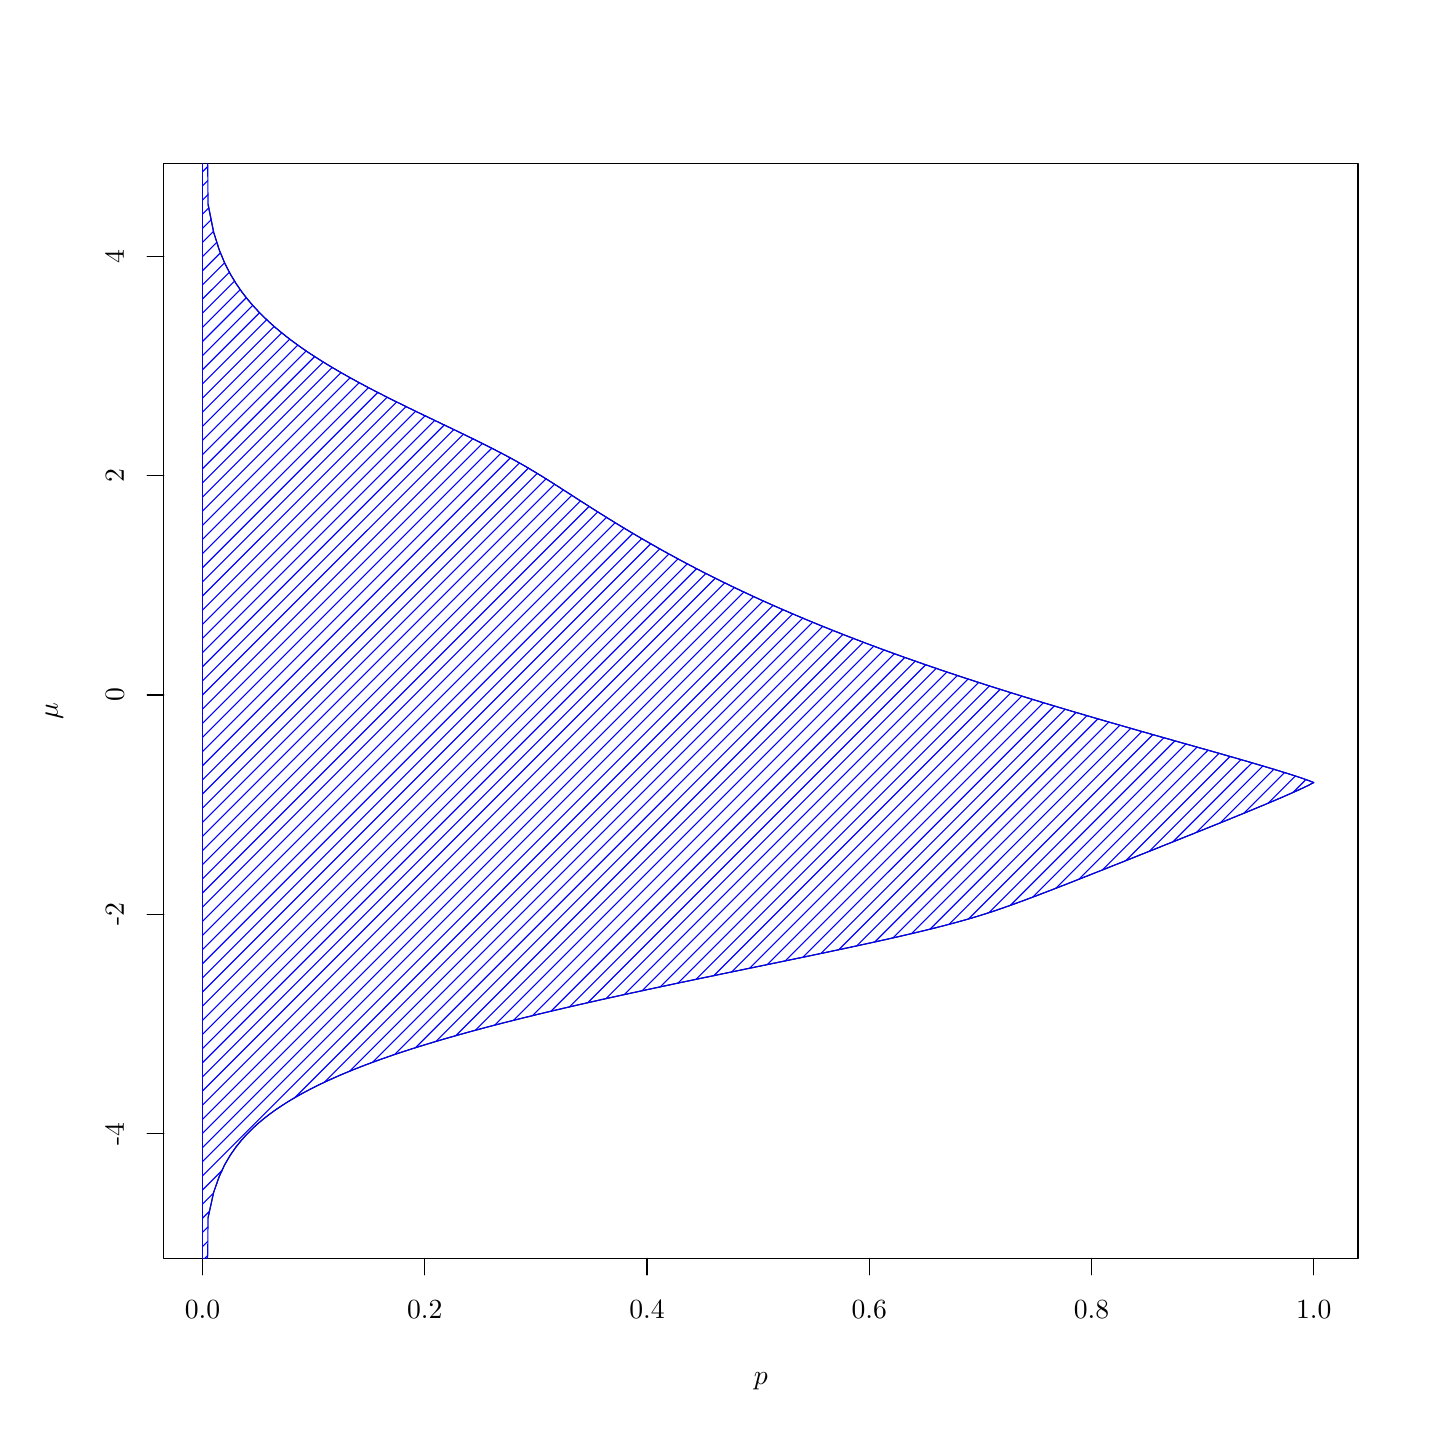
\begin{tikzpicture}[x=1pt,y=1pt]
\definecolor{fillColor}{RGB}{255,255,255}
\path[use as bounding box,fill=fillColor,fill opacity=0.00] (0,0) rectangle (505.89,505.89);
\begin{scope}
\path[clip] ( 49.20, 61.20) rectangle (480.69,456.69);
\definecolor{drawColor}{RGB}{0,0,0}

\path[draw=drawColor,line width= 0.4pt,line join=round,line cap=round] ( 65.18, 75.85) --
	( 67.19, 85.00) --
	( 69.20, 90.73) --
	( 71.20, 95.03) --
	( 73.21, 98.46) --
	( 75.22,101.35) --
	( 77.23,103.86) --
	( 79.23,106.08) --
	( 81.24,108.09) --
	( 83.25,109.92) --
	( 85.26,111.60) --
	( 87.27,113.16) --
	( 89.27,114.63) --
	( 91.28,116.00) --
	( 93.29,117.30) --
	( 95.30,118.53) --
	( 97.30,119.70) --
	( 99.31,120.82) --
	(101.32,121.89) --
	(103.33,122.92) --
	(105.33,123.92) --
	(107.34,124.88) --
	(109.35,125.80) --
	(111.36,126.70) --
	(113.37,127.57) --
	(115.37,128.41) --
	(117.38,129.23) --
	(119.39,130.03) --
	(121.40,130.81) --
	(123.40,131.57) --
	(125.41,132.31) --
	(127.42,133.04) --
	(129.43,133.74) --
	(131.43,134.44) --
	(133.44,135.12) --
	(135.45,135.79) --
	(137.46,136.44) --
	(139.47,137.09) --
	(141.47,137.72) --
	(143.48,138.34) --
	(145.49,138.95) --
	(147.50,139.56) --
	(149.50,140.15) --
	(151.51,140.74) --
	(153.52,141.31) --
	(155.53,141.88) --
	(157.53,142.44) --
	(159.54,143.00) --
	(161.55,143.54) --
	(163.56,144.08) --
	(165.56,144.62) --
	(167.57,145.15) --
	(169.58,145.67) --
	(171.59,146.19) --
	(173.60,146.70) --
	(175.60,147.20) --
	(177.61,147.71) --
	(179.62,148.20) --
	(181.63,148.69) --
	(183.63,149.18) --
	(185.64,149.67) --
	(187.65,150.15) --
	(189.66,150.62) --
	(191.66,151.09) --
	(193.67,151.56) --
	(195.68,152.03) --
	(197.69,152.49) --
	(199.70,152.95) --
	(201.70,153.41) --
	(203.71,153.86) --
	(205.72,154.31) --
	(207.73,154.76) --
	(209.73,155.21) --
	(211.74,155.65) --
	(213.75,156.09) --
	(215.76,156.53) --
	(217.76,156.97) --
	(219.77,157.40) --
	(221.78,157.83) --
	(223.79,158.27) --
	(225.80,158.69) --
	(227.80,159.12) --
	(229.81,159.55) --
	(231.82,159.97) --
	(233.83,160.40) --
	(235.83,160.82) --
	(237.84,161.24) --
	(239.85,161.66) --
	(241.86,162.08) --
	(243.86,162.50) --
	(245.87,162.91) --
	(247.88,163.33) --
	(249.89,163.75) --
	(251.90,164.16) --
	(253.90,164.58) --
	(255.91,164.99) --
	(257.92,165.41) --
	(259.93,165.82) --
	(261.93,166.23) --
	(263.94,166.65) --
	(265.95,167.06) --
	(267.96,167.47) --
	(269.96,167.89) --
	(271.97,168.30) --
	(273.98,168.72) --
	(275.99,169.13) --
	(277.99,169.55) --
	(280.00,169.96) --
	(282.01,170.38) --
	(284.02,170.80) --
	(286.03,171.22) --
	(288.03,171.64) --
	(290.04,172.06) --
	(292.05,172.49) --
	(294.06,172.91) --
	(296.06,173.34) --
	(298.07,173.77) --
	(300.08,174.20) --
	(302.09,174.64) --
	(304.09,175.07) --
	(306.10,175.51) --
	(308.11,175.96) --
	(310.12,176.40) --
	(312.13,176.86) --
	(314.13,177.31) --
	(316.14,177.77) --
	(318.15,178.24) --
	(320.16,178.71) --
	(322.16,179.19) --
	(324.17,179.67) --
	(326.18,180.16) --
	(328.19,180.66) --
	(330.19,181.17) --
	(332.20,181.69) --
	(334.21,182.22) --
	(336.22,182.77) --
	(338.23,183.33) --
	(340.23,183.90) --
	(342.24,184.49) --
	(344.25,185.11) --
	(346.26,185.74) --
	(348.26,186.39) --
	(350.27,187.06) --
	(352.28,187.75) --
	(354.29,188.45) --
	(356.29,189.17) --
	(358.30,189.90) --
	(360.31,190.64) --
	(362.32,191.39) --
	(364.33,192.14) --
	(366.33,192.91) --
	(368.34,193.68) --
	(370.35,194.45) --
	(372.36,195.23) --
	(374.36,196.01) --
	(376.37,196.80) --
	(378.38,197.59) --
	(380.39,198.38) --
	(382.39,199.17) --
	(384.40,199.96) --
	(386.41,200.76) --
	(388.42,201.56) --
	(390.42,202.35) --
	(392.43,203.15) --
	(394.44,203.95) --
	(396.45,204.75) --
	(398.46,205.55) --
	(400.46,206.35) --
	(402.47,207.15) --
	(404.48,207.95) --
	(406.49,208.75) --
	(408.49,209.55) --
	(410.50,210.36) --
	(412.51,211.16) --
	(414.52,211.96) --
	(416.52,212.76) --
	(418.53,213.57) --
	(420.54,214.37) --
	(422.55,215.18) --
	(424.56,215.98) --
	(426.56,216.79) --
	(428.57,217.60) --
	(430.58,218.41) --
	(432.59,219.22) --
	(434.59,220.03) --
	(436.60,220.85) --
	(438.61,221.67) --
	(440.62,222.49) --
	(442.62,223.31) --
	(444.63,224.15) --
	(446.64,224.98) --
	(448.65,225.82) --
	(450.66,226.67) --
	(452.66,227.53) --
	(454.67,228.40) --
	(456.68,229.28) --
	(458.69,230.18) --
	(460.69,231.10) --
	(462.70,232.06) --
	(464.71,233.11);
\end{scope}
\begin{scope}
\path[clip] (  0.00,  0.00) rectangle (505.89,505.89);
\definecolor{drawColor}{RGB}{0,0,0}

\path[draw=drawColor,line width= 0.4pt,line join=round,line cap=round] ( 63.17, 61.20) -- (464.71, 61.20);

\path[draw=drawColor,line width= 0.4pt,line join=round,line cap=round] ( 63.17, 61.20) -- ( 63.17, 55.20);

\path[draw=drawColor,line width= 0.4pt,line join=round,line cap=round] (143.48, 61.20) -- (143.48, 55.20);

\path[draw=drawColor,line width= 0.4pt,line join=round,line cap=round] (223.79, 61.20) -- (223.79, 55.20);

\path[draw=drawColor,line width= 0.4pt,line join=round,line cap=round] (304.09, 61.20) -- (304.09, 55.20);

\path[draw=drawColor,line width= 0.4pt,line join=round,line cap=round] (384.40, 61.20) -- (384.40, 55.20);

\path[draw=drawColor,line width= 0.4pt,line join=round,line cap=round] (464.71, 61.20) -- (464.71, 55.20);

\node[text=drawColor,anchor=base,inner sep=0pt, outer sep=0pt, scale=  1.00] at ( 63.17, 39.60) {0.0};

\node[text=drawColor,anchor=base,inner sep=0pt, outer sep=0pt, scale=  1.00] at (143.48, 39.60) {0.2};

\node[text=drawColor,anchor=base,inner sep=0pt, outer sep=0pt, scale=  1.00] at (223.79, 39.60) {0.4};

\node[text=drawColor,anchor=base,inner sep=0pt, outer sep=0pt, scale=  1.00] at (304.09, 39.60) {0.6};

\node[text=drawColor,anchor=base,inner sep=0pt, outer sep=0pt, scale=  1.00] at (384.40, 39.60) {0.8};

\node[text=drawColor,anchor=base,inner sep=0pt, outer sep=0pt, scale=  1.00] at (464.71, 39.60) {1.0};

\path[draw=drawColor,line width= 0.4pt,line join=round,line cap=round] ( 49.20,106.17) -- ( 49.20,423.30);

\path[draw=drawColor,line width= 0.4pt,line join=round,line cap=round] ( 49.20,106.17) -- ( 43.20,106.17);

\path[draw=drawColor,line width= 0.4pt,line join=round,line cap=round] ( 49.20,185.45) -- ( 43.20,185.45);

\path[draw=drawColor,line width= 0.4pt,line join=round,line cap=round] ( 49.20,264.74) -- ( 43.20,264.74);

\path[draw=drawColor,line width= 0.4pt,line join=round,line cap=round] ( 49.20,344.02) -- ( 43.20,344.02);

\path[draw=drawColor,line width= 0.4pt,line join=round,line cap=round] ( 49.20,423.30) -- ( 43.20,423.30);

\node[text=drawColor,rotate= 90.00,anchor=base,inner sep=0pt, outer sep=0pt, scale=  1.00] at ( 34.80,106.17) {-4};

\node[text=drawColor,rotate= 90.00,anchor=base,inner sep=0pt, outer sep=0pt, scale=  1.00] at ( 34.80,185.45) {-2};

\node[text=drawColor,rotate= 90.00,anchor=base,inner sep=0pt, outer sep=0pt, scale=  1.00] at ( 34.80,264.74) {0};

\node[text=drawColor,rotate= 90.00,anchor=base,inner sep=0pt, outer sep=0pt, scale=  1.00] at ( 34.80,344.02) {2};

\node[text=drawColor,rotate= 90.00,anchor=base,inner sep=0pt, outer sep=0pt, scale=  1.00] at ( 34.80,423.30) {4};

\path[draw=drawColor,line width= 0.4pt,line join=round,line cap=round] ( 49.20, 61.20) --
	(480.69, 61.20) --
	(480.69,456.69) --
	( 49.20,456.69) --
	( 49.20, 61.20);
\end{scope}
\begin{scope}
\path[clip] (  0.00,  0.00) rectangle (505.89,505.89);
\definecolor{drawColor}{RGB}{0,0,0}

\node[text=drawColor,anchor=base,inner sep=0pt, outer sep=0pt, scale=  1.00] at (264.94, 15.60) {$p$};

\node[text=drawColor,rotate= 90.00,anchor=base,inner sep=0pt, outer sep=0pt, scale=  1.00] at ( 10.80,258.94) {$\mu$};
\end{scope}
\begin{scope}
\path[clip] ( 49.20, 61.20) rectangle (480.69,456.69);
\definecolor{drawColor}{RGB}{0,0,0}

\path[draw=drawColor,line width= 0.4pt,line join=round,line cap=round] ( 65.18,442.04) --
	( 67.19,432.01) --
	( 69.20,425.64) --
	( 71.20,420.81) --
	( 73.21,416.88) --
	( 75.22,413.55) --
	( 77.23,410.62) --
	( 79.23,408.01) --
	( 81.24,405.64) --
	( 83.25,403.46) --
	( 85.26,401.42) --
	( 87.27,399.52) --
	( 89.27,397.73) --
	( 91.28,396.04) --
	( 93.29,394.42) --
	( 95.30,392.88) --
	( 97.30,391.40) --
	( 99.31,389.97) --
	(101.32,388.60) --
	(103.33,387.28) --
	(105.33,385.99) --
	(107.34,384.74) --
	(109.35,383.52) --
	(111.36,382.33) --
	(113.37,381.17) --
	(115.37,380.03) --
	(117.38,378.91) --
	(119.39,377.82) --
	(121.40,376.74) --
	(123.40,375.68) --
	(125.41,374.63) --
	(127.42,373.60) --
	(129.43,372.58) --
	(131.43,371.58) --
	(133.44,370.58) --
	(135.45,369.59) --
	(137.46,368.61) --
	(139.47,367.63) --
	(141.47,366.66) --
	(143.48,365.70) --
	(145.49,364.73) --
	(147.50,363.77) --
	(149.50,362.81) --
	(151.51,361.85) --
	(153.52,360.89) --
	(155.53,359.92) --
	(157.53,358.95) --
	(159.54,357.98) --
	(161.55,357.00) --
	(163.56,356.01) --
	(165.56,355.01) --
	(167.57,353.99) --
	(169.58,352.96) --
	(171.59,351.92) --
	(173.60,350.85) --
	(175.60,349.76) --
	(177.61,348.64) --
	(179.62,347.50) --
	(181.63,346.32) --
	(183.63,345.12) --
	(185.64,343.89) --
	(187.65,342.64) --
	(189.66,341.37) --
	(191.66,340.09) --
	(193.67,338.80) --
	(195.68,337.51) --
	(197.69,336.21) --
	(199.70,334.92) --
	(201.70,333.64) --
	(203.71,332.36) --
	(205.72,331.09) --
	(207.73,329.83) --
	(209.73,328.58) --
	(211.74,327.34) --
	(213.75,326.11) --
	(215.76,324.90) --
	(217.76,323.69) --
	(219.77,322.51) --
	(221.78,321.33) --
	(223.79,320.17) --
	(225.80,319.02) --
	(227.80,317.88) --
	(229.81,316.76) --
	(231.82,315.65) --
	(233.83,314.56) --
	(235.83,313.47) --
	(237.84,312.40) --
	(239.85,311.35) --
	(241.86,310.30) --
	(243.86,309.27) --
	(245.87,308.25) --
	(247.88,307.24) --
	(249.89,306.24) --
	(251.90,305.26) --
	(253.90,304.28) --
	(255.91,303.32) --
	(257.92,302.37) --
	(259.93,301.43) --
	(261.93,300.50) --
	(263.94,299.57) --
	(265.95,298.66) --
	(267.96,297.76) --
	(269.96,296.87) --
	(271.97,295.99) --
	(273.98,295.12) --
	(275.99,294.25) --
	(277.99,293.40) --
	(280.00,292.55) --
	(282.01,291.71) --
	(284.02,290.89) --
	(286.03,290.06) --
	(288.03,289.25) --
	(290.04,288.44) --
	(292.05,287.65) --
	(294.06,286.86) --
	(296.06,286.07) --
	(298.07,285.30) --
	(300.08,284.53) --
	(302.09,283.76) --
	(304.09,283.01) --
	(306.10,282.26) --
	(308.11,281.51) --
	(310.12,280.78) --
	(312.13,280.05) --
	(314.13,279.32) --
	(316.14,278.60) --
	(318.15,277.89) --
	(320.16,277.18) --
	(322.16,276.48) --
	(324.17,275.78) --
	(326.18,275.09) --
	(328.19,274.40) --
	(330.19,273.72) --
	(332.20,273.05) --
	(334.21,272.37) --
	(336.22,271.71) --
	(338.23,271.04) --
	(340.23,270.38) --
	(342.24,269.73) --
	(344.25,269.08) --
	(346.26,268.43) --
	(348.26,267.79) --
	(350.27,267.15) --
	(352.28,266.52) --
	(354.29,265.89) --
	(356.29,265.26) --
	(358.30,264.64) --
	(360.31,264.02) --
	(362.32,263.40) --
	(364.33,262.79) --
	(366.33,262.18) --
	(368.34,261.57) --
	(370.35,260.96) --
	(372.36,260.36) --
	(374.36,259.76) --
	(376.37,259.17) --
	(378.38,258.57) --
	(380.39,257.98) --
	(382.39,257.39) --
	(384.40,256.80) --
	(386.41,256.22) --
	(388.42,255.63) --
	(390.42,255.05) --
	(392.43,254.47) --
	(394.44,253.90) --
	(396.45,253.32) --
	(398.46,252.75) --
	(400.46,252.17) --
	(402.47,251.60) --
	(404.48,251.03) --
	(406.49,250.46) --
	(408.49,249.89) --
	(410.50,249.32) --
	(412.51,248.76) --
	(414.52,248.19) --
	(416.52,247.62) --
	(418.53,247.05) --
	(420.54,246.49) --
	(422.55,245.92) --
	(424.56,245.35) --
	(426.56,244.79) --
	(428.57,244.22) --
	(430.58,243.65) --
	(432.59,243.07) --
	(434.59,242.50) --
	(436.60,241.93) --
	(438.61,241.35) --
	(440.62,240.77) --
	(442.62,240.18) --
	(444.63,239.59) --
	(446.64,239.00) --
	(448.65,238.40) --
	(450.66,237.80) --
	(452.66,237.19) --
	(454.67,236.56) --
	(456.68,235.93) --
	(458.69,235.28) --
	(460.69,234.61) --
	(462.70,233.90) --
	(464.71,233.11);
\definecolor{drawColor}{RGB}{0,0,255}

\path[draw=drawColor,line width= 0.4pt,line join=round,line cap=round] ( 63.17,504.92) -- ( 64.14,505.89);

\path[draw=drawColor,line width= 0.4pt,line join=round,line cap=round] ( 63.17,499.81) -- ( 64.64,501.28);

\path[draw=drawColor,line width= 0.4pt,line join=round,line cap=round] ( 63.17,494.70) -- ( 64.68,496.21);

\path[draw=drawColor,line width= 0.4pt,line join=round,line cap=round] ( 63.17,489.59) -- ( 64.73,491.15);

\path[draw=drawColor,line width= 0.4pt,line join=round,line cap=round] ( 63.17,484.48) -- ( 64.78,486.08);

\path[draw=drawColor,line width= 0.4pt,line join=round,line cap=round] ( 63.17,479.37) -- ( 64.82,481.02);

\path[draw=drawColor,line width= 0.4pt,line join=round,line cap=round] ( 63.17,474.26) -- ( 64.87,475.96);

\path[draw=drawColor,line width= 0.4pt,line join=round,line cap=round] ( 63.17,469.15) -- ( 64.92,470.89);

\path[draw=drawColor,line width= 0.4pt,line join=round,line cap=round] ( 63.17,464.04) -- ( 64.96,465.83);

\path[draw=drawColor,line width= 0.4pt,line join=round,line cap=round] ( 63.17,458.93) -- ( 65.01,460.76);

\path[draw=drawColor,line width= 0.4pt,line join=round,line cap=round] ( 63.17,453.82) -- ( 65.06,455.70);

\path[draw=drawColor,line width= 0.4pt,line join=round,line cap=round] ( 63.17,448.71) -- ( 65.10,450.64);

\path[draw=drawColor,line width= 0.4pt,line join=round,line cap=round] ( 63.17,443.60) -- ( 65.15,445.57);

\path[draw=drawColor,line width= 0.4pt,line join=round,line cap=round] ( 63.17,438.49) -- ( 65.44,440.75);

\path[draw=drawColor,line width= 0.4pt,line join=round,line cap=round] ( 63.17,433.38) -- ( 66.29,436.49);

\path[draw=drawColor,line width= 0.4pt,line join=round,line cap=round] ( 63.17,428.27) -- ( 67.14,432.24);

\path[draw=drawColor,line width= 0.4pt,line join=round,line cap=round] ( 63.17,423.16) -- ( 68.35,428.33);

\path[draw=drawColor,line width= 0.4pt,line join=round,line cap=round] ( 63.17,418.05) -- ( 69.66,424.53);

\path[draw=drawColor,line width= 0.4pt,line join=round,line cap=round] ( 63.17,412.94) -- ( 71.16,420.92);

\path[draw=drawColor,line width= 0.4pt,line join=round,line cap=round] ( 63.17,407.83) -- ( 72.88,417.53);

\path[draw=drawColor,line width= 0.4pt,line join=round,line cap=round] ( 63.17,402.72) -- ( 74.76,414.31);

\path[draw=drawColor,line width= 0.4pt,line join=round,line cap=round] ( 63.17,397.60) -- ( 76.81,411.24);

\path[draw=drawColor,line width= 0.4pt,line join=round,line cap=round] ( 63.17,392.49) -- ( 79.00,408.32);

\path[draw=drawColor,line width= 0.4pt,line join=round,line cap=round] ( 63.17,387.38) -- ( 81.33,405.54);

\path[draw=drawColor,line width= 0.4pt,line join=round,line cap=round] ( 63.17,382.27) -- ( 83.80,402.90);

\path[draw=drawColor,line width= 0.4pt,line join=round,line cap=round] ( 63.17,377.16) -- ( 86.38,400.37);

\path[draw=drawColor,line width= 0.4pt,line join=round,line cap=round] ( 63.17,372.05) -- ( 89.05,397.93);

\path[draw=drawColor,line width= 0.4pt,line join=round,line cap=round] ( 63.17,366.94) -- ( 91.83,395.60);

\path[draw=drawColor,line width= 0.4pt,line join=round,line cap=round] ( 63.17,361.83) -- ( 94.69,393.35);

\path[draw=drawColor,line width= 0.4pt,line join=round,line cap=round] ( 63.17,356.72) -- ( 97.62,391.17);

\path[draw=drawColor,line width= 0.4pt,line join=round,line cap=round] ( 63.17,351.61) -- (100.63,389.07);

\path[draw=drawColor,line width= 0.4pt,line join=round,line cap=round] ( 63.17,346.50) -- (103.71,387.03);

\path[draw=drawColor,line width= 0.4pt,line join=round,line cap=round] ( 63.17,341.39) -- (106.84,385.05);

\path[draw=drawColor,line width= 0.4pt,line join=round,line cap=round] ( 63.17,336.28) -- (110.02,383.12);

\path[draw=drawColor,line width= 0.4pt,line join=round,line cap=round] ( 63.17,331.17) -- (113.24,381.24);

\path[draw=drawColor,line width= 0.4pt,line join=round,line cap=round] ( 63.17,326.06) -- (116.51,379.40);

\path[draw=drawColor,line width= 0.4pt,line join=round,line cap=round] ( 63.17,320.95) -- (119.81,377.59);

\path[draw=drawColor,line width= 0.4pt,line join=round,line cap=round] ( 63.17,315.84) -- (123.15,375.81);

\path[draw=drawColor,line width= 0.4pt,line join=round,line cap=round] ( 63.17,310.73) -- (126.51,374.07);

\path[draw=drawColor,line width= 0.4pt,line join=round,line cap=round] ( 63.17,305.62) -- (129.90,372.35);

\path[draw=drawColor,line width= 0.4pt,line join=round,line cap=round] ( 63.17,300.51) -- (133.31,370.64);

\path[draw=drawColor,line width= 0.4pt,line join=round,line cap=round] ( 63.17,295.40) -- (136.74,368.96);

\path[draw=drawColor,line width= 0.4pt,line join=round,line cap=round] ( 63.17,290.29) -- (140.17,367.29);

\path[draw=drawColor,line width= 0.4pt,line join=round,line cap=round] ( 63.17,285.18) -- (143.62,365.63);

\path[draw=drawColor,line width= 0.4pt,line join=round,line cap=round] ( 63.17,280.07) -- (147.08,363.97);

\path[draw=drawColor,line width= 0.4pt,line join=round,line cap=round] ( 63.17,274.96) -- (150.53,362.32);

\path[draw=drawColor,line width= 0.4pt,line join=round,line cap=round] ( 63.17,269.85) -- (153.99,360.66);

\path[draw=drawColor,line width= 0.4pt,line join=round,line cap=round] ( 63.17,264.74) -- (157.44,359.00);

\path[draw=drawColor,line width= 0.4pt,line join=round,line cap=round] ( 63.17,259.63) -- (160.87,357.33);

\path[draw=drawColor,line width= 0.4pt,line join=round,line cap=round] ( 63.17,254.52) -- (164.30,355.64);

\path[draw=drawColor,line width= 0.4pt,line join=round,line cap=round] ( 63.17,249.41) -- (167.70,353.93);

\path[draw=drawColor,line width= 0.4pt,line join=round,line cap=round] ( 63.17,244.30) -- (171.07,352.19);

\path[draw=drawColor,line width= 0.4pt,line join=round,line cap=round] ( 63.17,239.19) -- (174.40,350.41);

\path[draw=drawColor,line width= 0.4pt,line join=round,line cap=round] ( 63.17,234.08) -- (177.69,348.59);

\path[draw=drawColor,line width= 0.4pt,line join=round,line cap=round] ( 63.17,228.97) -- (180.93,346.73);

\path[draw=drawColor,line width= 0.4pt,line join=round,line cap=round] ( 63.17,223.86) -- (184.13,344.82);

\path[draw=drawColor,line width= 0.4pt,line join=round,line cap=round] ( 63.17,218.75) -- (187.29,342.86);

\path[draw=drawColor,line width= 0.4pt,line join=round,line cap=round] ( 63.17,213.64) -- (190.42,340.88);

\path[draw=drawColor,line width= 0.4pt,line join=round,line cap=round] ( 63.17,208.53) -- (193.54,338.89);

\path[draw=drawColor,line width= 0.4pt,line join=round,line cap=round] ( 63.17,203.42) -- (196.64,336.89);

\path[draw=drawColor,line width= 0.4pt,line join=round,line cap=round] ( 63.17,198.30) -- (199.75,334.89);

\path[draw=drawColor,line width= 0.4pt,line join=round,line cap=round] ( 63.17,193.19) -- (202.87,332.89);

\path[draw=drawColor,line width= 0.4pt,line join=round,line cap=round] ( 63.17,188.08) -- (206.00,330.91);

\path[draw=drawColor,line width= 0.4pt,line join=round,line cap=round] ( 63.17,182.97) -- (209.14,328.94);

\path[draw=drawColor,line width= 0.4pt,line join=round,line cap=round] ( 63.17,177.86) -- (212.30,326.99);

\path[draw=drawColor,line width= 0.4pt,line join=round,line cap=round] ( 63.17,172.75) -- (215.48,325.06);

\path[draw=drawColor,line width= 0.4pt,line join=round,line cap=round] ( 63.17,167.64) -- (218.68,323.15);

\path[draw=drawColor,line width= 0.4pt,line join=round,line cap=round] ( 63.17,162.53) -- (221.90,321.26);

\path[draw=drawColor,line width= 0.4pt,line join=round,line cap=round] ( 63.17,157.42) -- (225.14,319.39);

\path[draw=drawColor,line width= 0.4pt,line join=round,line cap=round] ( 63.17,152.31) -- (228.41,317.55);

\path[draw=drawColor,line width= 0.4pt,line join=round,line cap=round] ( 63.17,147.20) -- (231.69,315.72);

\path[draw=drawColor,line width= 0.4pt,line join=round,line cap=round] ( 63.17,142.09) -- (235.00,313.92);

\path[draw=drawColor,line width= 0.4pt,line join=round,line cap=round] ( 63.17,136.98) -- (238.34,312.14);

\path[draw=drawColor,line width= 0.4pt,line join=round,line cap=round] ( 63.17,131.87) -- (241.69,310.39);

\path[draw=drawColor,line width= 0.4pt,line join=round,line cap=round] ( 63.17,126.76) -- (245.07,308.66);

\path[draw=drawColor,line width= 0.4pt,line join=round,line cap=round] ( 63.17,121.65) -- (248.47,306.95);

\path[draw=drawColor,line width= 0.4pt,line join=round,line cap=round] ( 63.17,116.54) -- (251.89,305.26);

\path[draw=drawColor,line width= 0.4pt,line join=round,line cap=round] ( 63.17,111.43) -- (255.34,303.60);

\path[draw=drawColor,line width= 0.4pt,line join=round,line cap=round] ( 63.17,106.32) -- (258.81,301.95);

\path[draw=drawColor,line width= 0.4pt,line join=round,line cap=round] ( 63.17,101.21) -- (262.29,300.33);

\path[draw=drawColor,line width= 0.4pt,line join=round,line cap=round] ( 63.17, 96.10) -- (265.80,298.73);

\path[draw=drawColor,line width= 0.4pt,line join=round,line cap=round] ( 63.17, 90.99) -- (269.34,297.15);

\path[draw=drawColor,line width= 0.4pt,line join=round,line cap=round] ( 63.17, 85.88) -- ( 70.23, 92.93);

\path[draw=drawColor,line width= 0.4pt,line join=round,line cap=round] ( 96.55,119.26) -- (272.89,295.59);

\path[draw=drawColor,line width= 0.4pt,line join=round,line cap=round] ( 63.17, 80.77) -- ( 67.13, 84.72);

\path[draw=drawColor,line width= 0.4pt,line join=round,line cap=round] (107.23,124.82) -- (276.46,294.05);

\path[draw=drawColor,line width= 0.4pt,line join=round,line cap=round] ( 63.17, 75.66) -- ( 65.69, 78.18);

\path[draw=drawColor,line width= 0.4pt,line join=round,line cap=round] (116.31,128.79) -- (280.05,292.53);

\path[draw=drawColor,line width= 0.4pt,line join=round,line cap=round] ( 63.17, 70.55) -- ( 65.15, 72.52);

\path[draw=drawColor,line width= 0.4pt,line join=round,line cap=round] (124.66,132.03) -- (283.66,291.03);

\path[draw=drawColor,line width= 0.4pt,line join=round,line cap=round] ( 63.17, 65.44) -- ( 65.10, 67.36);

\path[draw=drawColor,line width= 0.4pt,line join=round,line cap=round] (132.56,134.82) -- (287.29,289.55);

\path[draw=drawColor,line width= 0.4pt,line join=round,line cap=round] ( 63.17, 60.33) -- ( 65.05, 62.20);

\path[draw=drawColor,line width= 0.4pt,line join=round,line cap=round] (140.15,137.30) -- (290.93,288.09);

\path[draw=drawColor,line width= 0.4pt,line join=round,line cap=round] ( 63.17, 55.22) -- ( 65.00, 57.04);

\path[draw=drawColor,line width= 0.4pt,line join=round,line cap=round] (147.52,139.56) -- (294.60,286.64);

\path[draw=drawColor,line width= 0.4pt,line join=round,line cap=round] ( 63.17, 50.11) -- ( 64.95, 51.88);

\path[draw=drawColor,line width= 0.4pt,line join=round,line cap=round] (154.72,141.65) -- (298.28,285.22);

\path[draw=drawColor,line width= 0.4pt,line join=round,line cap=round] ( 63.17, 45.00) -- ( 64.90, 46.72);

\path[draw=drawColor,line width= 0.4pt,line join=round,line cap=round] (161.78,143.61) -- (301.98,283.80);

\path[draw=drawColor,line width= 0.4pt,line join=round,line cap=round] ( 63.17, 39.89) -- ( 64.85, 41.56);

\path[draw=drawColor,line width= 0.4pt,line join=round,line cap=round] (168.74,145.45) -- (305.70,282.41);

\path[draw=drawColor,line width= 0.4pt,line join=round,line cap=round] ( 63.17, 34.78) -- ( 64.80, 36.40);

\path[draw=drawColor,line width= 0.4pt,line join=round,line cap=round] (175.60,147.20) -- (309.43,281.03);

\path[draw=drawColor,line width= 0.4pt,line join=round,line cap=round] ( 63.17, 29.67) -- ( 64.75, 31.24);

\path[draw=drawColor,line width= 0.4pt,line join=round,line cap=round] (182.39,148.88) -- (313.17,279.67);

\path[draw=drawColor,line width= 0.4pt,line join=round,line cap=round] ( 63.17, 24.56) -- ( 64.70, 26.08);

\path[draw=drawColor,line width= 0.4pt,line join=round,line cap=round] (189.11,150.49) -- (316.94,278.32);

\path[draw=drawColor,line width= 0.4pt,line join=round,line cap=round] ( 63.17, 19.45) -- ( 64.65, 20.92);

\path[draw=drawColor,line width= 0.4pt,line join=round,line cap=round] (195.78,152.05) -- (320.71,276.99);

\path[draw=drawColor,line width= 0.4pt,line join=round,line cap=round] ( 63.17, 14.34) -- ( 64.60, 15.76);

\path[draw=drawColor,line width= 0.4pt,line join=round,line cap=round] (202.41,153.57) -- (324.51,275.67);

\path[draw=drawColor,line width= 0.4pt,line join=round,line cap=round] ( 63.17,  9.23) -- ( 64.55, 10.60);

\path[draw=drawColor,line width= 0.4pt,line join=round,line cap=round] (208.99,155.04) -- (328.31,274.36);

\path[draw=drawColor,line width= 0.4pt,line join=round,line cap=round] ( 63.17,  4.11) -- ( 64.50,  5.44);

\path[draw=drawColor,line width= 0.4pt,line join=round,line cap=round] (215.54,156.48) -- (332.13,273.07);

\path[draw=drawColor,line width= 0.4pt,line join=round,line cap=round] ( 64.17,  0.00) -- ( 64.45,  0.28);

\path[draw=drawColor,line width= 0.4pt,line join=round,line cap=round] (222.06,157.90) -- (335.96,271.79);

\path[draw=drawColor,line width= 0.4pt,line join=round,line cap=round] (228.56,159.28) -- (339.80,270.53);

\path[draw=drawColor,line width= 0.4pt,line join=round,line cap=round] (235.04,160.65) -- (343.66,269.27);

\path[draw=drawColor,line width= 0.4pt,line join=round,line cap=round] (241.51,162.01) -- (347.53,268.03);

\path[draw=drawColor,line width= 0.4pt,line join=round,line cap=round] (247.96,163.35) -- (351.40,266.80);

\path[draw=drawColor,line width= 0.4pt,line join=round,line cap=round] (254.40,164.68) -- (355.29,265.57);

\path[draw=drawColor,line width= 0.4pt,line join=round,line cap=round] (260.84,166.01) -- (359.19,264.36);

\path[draw=drawColor,line width= 0.4pt,line join=round,line cap=round] (267.27,167.33) -- (363.10,263.16);

\path[draw=drawColor,line width= 0.4pt,line join=round,line cap=round] (273.71,168.66) -- (367.02,261.97);

\path[draw=drawColor,line width= 0.4pt,line join=round,line cap=round] (280.16,170.00) -- (370.95,260.78);

\path[draw=drawColor,line width= 0.4pt,line join=round,line cap=round] (286.61,171.34) -- (374.88,259.61);

\path[draw=drawColor,line width= 0.4pt,line join=round,line cap=round] (293.09,172.71) -- (378.82,258.44);

\path[draw=drawColor,line width= 0.4pt,line join=round,line cap=round] (299.59,174.09) -- (382.77,257.28);

\path[draw=drawColor,line width= 0.4pt,line join=round,line cap=round] (306.12,175.52) -- (386.73,256.13);

\path[draw=drawColor,line width= 0.4pt,line join=round,line cap=round] (312.70,176.99) -- (390.69,254.98);

\path[draw=drawColor,line width= 0.4pt,line join=round,line cap=round] (319.34,178.52) -- (394.66,253.83);

\path[draw=drawColor,line width= 0.4pt,line join=round,line cap=round] (326.07,180.13) -- (398.63,252.70);

\path[draw=drawColor,line width= 0.4pt,line join=round,line cap=round] (332.93,181.88) -- (402.61,251.56);

\path[draw=drawColor,line width= 0.4pt,line join=round,line cap=round] (339.98,183.83) -- (406.59,250.43);

\path[draw=drawColor,line width= 0.4pt,line join=round,line cap=round] (347.36,186.10) -- (410.57,249.30);

\path[draw=drawColor,line width= 0.4pt,line join=round,line cap=round] (355.12,188.75) -- (414.55,248.18);

\path[draw=drawColor,line width= 0.4pt,line join=round,line cap=round] (363.21,191.72) -- (418.54,247.05);

\path[draw=drawColor,line width= 0.4pt,line join=round,line cap=round] (371.49,194.90) -- (422.52,245.93);

\path[draw=drawColor,line width= 0.4pt,line join=round,line cap=round] (379.88,198.18) -- (426.51,244.80);

\path[draw=drawColor,line width= 0.4pt,line join=round,line cap=round] (388.34,201.53) -- (430.49,243.67);

\path[draw=drawColor,line width= 0.4pt,line join=round,line cap=round] (396.83,204.90) -- (434.46,242.54);

\path[draw=drawColor,line width= 0.4pt,line join=round,line cap=round] (405.32,208.29) -- (438.43,241.40);

\path[draw=drawColor,line width= 0.4pt,line join=round,line cap=round] (413.83,211.69) -- (442.40,240.25);

\path[draw=drawColor,line width= 0.4pt,line join=round,line cap=round] (422.35,215.10) -- (446.34,239.09);

\path[draw=drawColor,line width= 0.4pt,line join=round,line cap=round] (430.90,218.54) -- (450.28,237.91);

\path[draw=drawColor,line width= 0.4pt,line join=round,line cap=round] (439.51,222.04) -- (454.19,236.71);

\path[draw=drawColor,line width= 0.4pt,line join=round,line cap=round] (448.24,225.65) -- (458.07,235.48);

\path[draw=drawColor,line width= 0.4pt,line join=round,line cap=round] (457.22,229.52) -- (461.88,234.19);

\path[draw=drawColor,line width= 0.4pt,line join=round,line cap=round] ( 64.45,  0.00) --
	( 65.18, 75.85) --
	( 67.19, 85.00) --
	( 69.20, 90.73) --
	( 71.20, 95.03) --
	( 73.21, 98.46) --
	( 75.22,101.35) --
	( 77.23,103.86) --
	( 79.23,106.08) --
	( 81.24,108.09) --
	( 83.25,109.92) --
	( 85.26,111.60) --
	( 87.27,113.16) --
	( 89.27,114.63) --
	( 91.28,116.00) --
	( 93.29,117.30) --
	( 95.30,118.53) --
	( 97.30,119.70) --
	( 99.31,120.82) --
	(101.32,121.89) --
	(103.33,122.92) --
	(105.33,123.92) --
	(107.34,124.88) --
	(109.35,125.80) --
	(111.36,126.70) --
	(113.37,127.57) --
	(115.37,128.41) --
	(117.38,129.23) --
	(119.39,130.03) --
	(121.40,130.81) --
	(123.40,131.57) --
	(125.41,132.31) --
	(127.42,133.04) --
	(129.43,133.74) --
	(131.43,134.44) --
	(133.44,135.12) --
	(135.45,135.79) --
	(137.46,136.44) --
	(139.47,137.09) --
	(141.47,137.72) --
	(143.48,138.34) --
	(145.49,138.95) --
	(147.50,139.56) --
	(149.50,140.15) --
	(151.51,140.74) --
	(153.52,141.31) --
	(155.53,141.88) --
	(157.53,142.44) --
	(159.54,143.00) --
	(161.55,143.54) --
	(163.56,144.08) --
	(165.56,144.62) --
	(167.57,145.15) --
	(169.58,145.67) --
	(171.59,146.19) --
	(173.60,146.70) --
	(175.60,147.20) --
	(177.61,147.71) --
	(179.62,148.20) --
	(181.63,148.69) --
	(183.63,149.18) --
	(185.64,149.67) --
	(187.65,150.15) --
	(189.66,150.62) --
	(191.66,151.09) --
	(193.67,151.56) --
	(195.68,152.03) --
	(197.69,152.49) --
	(199.70,152.95) --
	(201.70,153.41) --
	(203.71,153.86) --
	(205.72,154.31) --
	(207.73,154.76) --
	(209.73,155.21) --
	(211.74,155.65) --
	(213.75,156.09) --
	(215.76,156.53) --
	(217.76,156.97) --
	(219.77,157.40) --
	(221.78,157.83) --
	(223.79,158.27) --
	(225.80,158.69) --
	(227.80,159.12) --
	(229.81,159.55) --
	(231.82,159.97) --
	(233.83,160.40) --
	(235.83,160.82) --
	(237.84,161.24) --
	(239.85,161.66) --
	(241.86,162.08) --
	(243.86,162.50) --
	(245.87,162.91) --
	(247.88,163.33) --
	(249.89,163.75) --
	(251.90,164.16) --
	(253.90,164.58) --
	(255.91,164.99) --
	(257.92,165.41) --
	(259.93,165.82) --
	(261.93,166.23) --
	(263.94,166.65) --
	(265.95,167.06) --
	(267.96,167.47) --
	(269.96,167.89) --
	(271.97,168.30) --
	(273.98,168.72) --
	(275.99,169.13) --
	(277.99,169.55) --
	(280.00,169.96) --
	(282.01,170.38) --
	(284.02,170.80) --
	(286.03,171.22) --
	(288.03,171.64) --
	(290.04,172.06) --
	(292.05,172.49) --
	(294.06,172.91) --
	(296.06,173.34) --
	(298.07,173.77) --
	(300.08,174.20) --
	(302.09,174.64) --
	(304.09,175.07) --
	(306.10,175.51) --
	(308.11,175.96) --
	(310.12,176.40) --
	(312.13,176.86) --
	(314.13,177.31) --
	(316.14,177.77) --
	(318.15,178.24) --
	(320.16,178.71) --
	(322.16,179.19) --
	(324.17,179.67) --
	(326.18,180.16) --
	(328.19,180.66) --
	(330.19,181.17) --
	(332.20,181.69) --
	(334.21,182.22) --
	(336.22,182.77) --
	(338.23,183.33) --
	(340.23,183.90) --
	(342.24,184.49) --
	(344.25,185.11) --
	(346.26,185.74) --
	(348.26,186.39) --
	(350.27,187.06) --
	(352.28,187.75) --
	(354.29,188.45) --
	(356.29,189.17) --
	(358.30,189.90) --
	(360.31,190.64) --
	(362.32,191.39) --
	(364.33,192.14) --
	(366.33,192.91) --
	(368.34,193.68) --
	(370.35,194.45) --
	(372.36,195.23) --
	(374.36,196.01) --
	(376.37,196.80) --
	(378.38,197.59) --
	(380.39,198.38) --
	(382.39,199.17) --
	(384.40,199.96) --
	(386.41,200.76) --
	(388.42,201.56) --
	(390.42,202.35) --
	(392.43,203.15) --
	(394.44,203.95) --
	(396.45,204.75) --
	(398.46,205.55) --
	(400.46,206.35) --
	(402.47,207.15) --
	(404.48,207.95) --
	(406.49,208.75) --
	(408.49,209.55) --
	(410.50,210.36) --
	(412.51,211.16) --
	(414.52,211.96) --
	(416.52,212.76) --
	(418.53,213.57) --
	(420.54,214.37) --
	(422.55,215.18) --
	(424.56,215.98) --
	(426.56,216.79) --
	(428.57,217.60) --
	(430.58,218.41) --
	(432.59,219.22) --
	(434.59,220.03) --
	(436.60,220.85) --
	(438.61,221.67) --
	(440.62,222.49) --
	(442.62,223.31) --
	(444.63,224.15) --
	(446.64,224.98) --
	(448.65,225.82) --
	(450.66,226.67) --
	(452.66,227.53) --
	(454.67,228.40) --
	(456.68,229.28) --
	(458.69,230.18) --
	(460.69,231.10) --
	(462.70,232.06) --
	(464.71,233.11) --
	(464.71,233.11) --
	(462.70,233.90) --
	(460.69,234.61) --
	(458.69,235.28) --
	(456.68,235.93) --
	(454.67,236.56) --
	(452.66,237.19) --
	(450.66,237.80) --
	(448.65,238.40) --
	(446.64,239.00) --
	(444.63,239.59) --
	(442.62,240.18) --
	(440.62,240.77) --
	(438.61,241.35) --
	(436.60,241.93) --
	(434.59,242.50) --
	(432.59,243.07) --
	(430.58,243.65) --
	(428.57,244.22) --
	(426.56,244.79) --
	(424.56,245.35) --
	(422.55,245.92) --
	(420.54,246.49) --
	(418.53,247.05) --
	(416.52,247.62) --
	(414.52,248.19) --
	(412.51,248.76) --
	(410.50,249.32) --
	(408.49,249.89) --
	(406.49,250.46) --
	(404.48,251.03) --
	(402.47,251.60) --
	(400.46,252.17) --
	(398.46,252.75) --
	(396.45,253.32) --
	(394.44,253.90) --
	(392.43,254.47) --
	(390.42,255.05) --
	(388.42,255.63) --
	(386.41,256.22) --
	(384.40,256.80) --
	(382.39,257.39) --
	(380.39,257.98) --
	(378.38,258.57) --
	(376.37,259.17) --
	(374.36,259.76) --
	(372.36,260.36) --
	(370.35,260.96) --
	(368.34,261.57) --
	(366.33,262.18) --
	(364.33,262.79) --
	(362.32,263.40) --
	(360.31,264.02) --
	(358.30,264.64) --
	(356.29,265.26) --
	(354.29,265.89) --
	(352.28,266.52) --
	(350.27,267.15) --
	(348.26,267.79) --
	(346.26,268.43) --
	(344.25,269.08) --
	(342.24,269.73) --
	(340.23,270.38) --
	(338.23,271.04) --
	(336.22,271.71) --
	(334.21,272.37) --
	(332.20,273.05) --
	(330.19,273.72) --
	(328.19,274.40) --
	(326.18,275.09) --
	(324.17,275.78) --
	(322.16,276.48) --
	(320.16,277.18) --
	(318.15,277.89) --
	(316.14,278.60) --
	(314.13,279.32) --
	(312.13,280.05) --
	(310.12,280.78) --
	(308.11,281.51) --
	(306.10,282.26) --
	(304.09,283.01) --
	(302.09,283.76) --
	(300.08,284.53) --
	(298.07,285.30) --
	(296.06,286.07) --
	(294.06,286.86) --
	(292.05,287.65) --
	(290.04,288.44) --
	(288.03,289.25) --
	(286.03,290.06) --
	(284.02,290.89) --
	(282.01,291.71) --
	(280.00,292.55) --
	(277.99,293.40) --
	(275.99,294.25) --
	(273.98,295.12) --
	(271.97,295.99) --
	(269.96,296.87) --
	(267.96,297.76) --
	(265.95,298.66) --
	(263.94,299.57) --
	(261.93,300.50) --
	(259.93,301.43) --
	(257.92,302.37) --
	(255.91,303.32) --
	(253.90,304.28) --
	(251.90,305.26) --
	(249.89,306.24) --
	(247.88,307.24) --
	(245.87,308.25) --
	(243.86,309.27) --
	(241.86,310.30) --
	(239.85,311.35) --
	(237.84,312.40) --
	(235.83,313.47) --
	(233.83,314.56) --
	(231.82,315.65) --
	(229.81,316.76) --
	(227.80,317.88) --
	(225.80,319.02) --
	(223.79,320.17) --
	(221.78,321.33) --
	(219.77,322.51) --
	(217.76,323.69) --
	(215.76,324.90) --
	(213.75,326.11) --
	(211.74,327.34) --
	(209.73,328.58) --
	(207.73,329.83) --
	(205.72,331.09) --
	(203.71,332.36) --
	(201.70,333.64) --
	(199.70,334.92) --
	(197.69,336.21) --
	(195.68,337.51) --
	(193.67,338.80) --
	(191.66,340.09) --
	(189.66,341.37) --
	(187.65,342.64) --
	(185.64,343.89) --
	(183.63,345.12) --
	(181.63,346.32) --
	(179.62,347.50) --
	(177.61,348.64) --
	(175.60,349.76) --
	(173.60,350.85) --
	(171.59,351.92) --
	(169.58,352.96) --
	(167.57,353.99) --
	(165.56,355.01) --
	(163.56,356.01) --
	(161.55,357.00) --
	(159.54,357.98) --
	(157.53,358.95) --
	(155.53,359.92) --
	(153.52,360.89) --
	(151.51,361.85) --
	(149.50,362.81) --
	(147.50,363.77) --
	(145.49,364.73) --
	(143.48,365.70) --
	(141.47,366.66) --
	(139.47,367.63) --
	(137.46,368.61) --
	(135.45,369.59) --
	(133.44,370.58) --
	(131.43,371.58) --
	(129.43,372.58) --
	(127.42,373.60) --
	(125.41,374.63) --
	(123.40,375.68) --
	(121.40,376.74) --
	(119.39,377.82) --
	(117.38,378.91) --
	(115.37,380.03) --
	(113.37,381.17) --
	(111.36,382.33) --
	(109.35,383.52) --
	(107.34,384.74) --
	(105.33,385.99) --
	(103.33,387.28) --
	(101.32,388.60) --
	( 99.31,389.97) --
	( 97.30,391.40) --
	( 95.30,392.88) --
	( 93.29,394.42) --
	( 91.28,396.04) --
	( 89.27,397.73) --
	( 87.27,399.52) --
	( 85.26,401.42) --
	( 83.25,403.46) --
	( 81.24,405.64) --
	( 79.23,408.01) --
	( 77.23,410.62) --
	( 75.22,413.55) --
	( 73.21,416.88) --
	( 71.20,420.81) --
	( 69.20,425.64) --
	( 67.19,432.01) --
	( 65.18,442.04) --
	( 64.60,505.89);

\path[draw=drawColor,line width= 0.4pt,line join=round,line cap=round] ( 63.17,505.89) --
	( 63.17,  0.00);
\end{scope}
\end{tikzpicture}

}
\end{figure}


  \note{\singlespacing\footnotesize
    \begin{itemize}
      \item For this particular choice of $f$, a mixture of normals, the blue shaded region shows all pairs $(p, \mu)$ that are compatible with the mixture.
      \item If $p=0$, $\mu$ is unconstrained. This makes sense: in this case $H$ can have any mean because it contributes nothing to the mixture that generates $F$.
      \item If $p=1$ then $\mu$ must \emph{equal} the mean of the observed distribution $F$, here $-0.8$, since this is a degenerate mixture where $F=H$.
      \item Relation to original problem? We observe dist of $y|T,z$ which is related to the unobserved dist of $y|T,T^*,z$ via a mixture model. Mixing prob.\  depends only on observables and $(\alpha_0, \alpha_1)$; same for means of mixture components. Hence, some values of $(\alpha_0, \alpha_1)$ are incompatible with the mixture model.
        This in restricts $\beta$ since IV is $\beta/(1 - \alpha_0 - \alpha_1)$. Joint restrictions for all $(t,k)$ so the book-keeping is complicated, but intuition is same as in simple mixture of normals example.
    \end{itemize}
  }%

\end{frame}
%%%%%%%%%%%%%%%%%%%%%%%%%%%%%%%%%%%%%%%%%%%%%%%%%%%%%
\begin{frame}
  \frametitle{Sharp Identified Set under Baseline Assumptions}


  \begin{alertblock}{Theorem}
    \begin{enumerate}[(i)]
      \item If $\mathbb{E}[y|\mathbf{x},T=0,z=k] \neq \mathbb{E}[y|\mathbf{x},T=1,z=k]$ for some $k$, non-differential assump.\ strictly improves upon weak bounds.
      \item Under the baseline assumptions, $\beta$ is not point identified, regardless of how many (discrete) values $z$ takes on.
    \end{enumerate}
  \end{alertblock}


  \begin{block}{Corollary}
    Bounds for $\alpha_0, \alpha_1$, and $\beta$ remain valid in a LATE model. They may not be sharp, however, sharp, since they do not incorporate the testable implications of the LATE assumptions.
  \end{block}

  \note{\singlespacing\footnotesize
    \begin{itemize}
      \item Second main contribution: sharp identified set for $(\alpha_0, \alpha_1, \beta)$ under baseline assumptions. Description of sharp set complicated, so I won't show it. But the form that this set takes leads to two important results. First, non-differential assumption \emph{generically} improves upon the weak bounds. Second, under the baseline assumptions $\beta$ is \emph{never} point identified, regardless of how many different (discrete) values $z$ takes.
      %\item Some intuition: the true $\beta$ always lies within the identified set by definition. It turns out that $\alpha_0 = \alpha_1 = 0$ implies that the mixing probabilities $r_{tk}$ are all either zero or one. But in this case the mixtures are trivial, so we can simply set $F = H$. Hence, the IV estimand always lies in the sharp identified set.
      \item Corollary: everything I've said so far concerns an additively separable model. But in fact, bounds we derive under the baseline assumptions remain valid if we re-state our assumptions so that they involve a LATE model. These bounds may not be sharp in a LATE model, however, because the LATE assumptions themselves have testable implications. We don't impose these since we're mainly interested in the add.\ sep.\ case.
      \item What now? Sharp bounds quite informative in practice, but don't point identify $\beta$.
        Baseline assumptions aren't enough. Slightly stronger but still plausible assumptions that point identify $\beta$? Yes! 
    \end{itemize}
  }%


\end{frame}
%%%%%%%%%%%%%%%%%%%%%%%%%%%%%%%%%%%%%%%%%%%%%%%%%%%%
\begin{frame}
  \frametitle{Point Identification: 1st Ingredient}



  \begin{block}{Reparameterization}
    \vspace{-1em}
\begin{align*}
  \theta_1(\mathbf{x}) &= \beta(\mathbf{x})/\left[ 1 - \alpha_0(\mathbf{x}) - \mathbf{\alpha}_1(\mathbf{x})  \right]\\
  \theta_2(\mathbf{x}) &= \left[\theta_1(\mathbf{x})\right]^2 \left[ 1 + \alpha_0(\mathbf{x}) - \alpha_1(\mathbf{x})\right] \\
  \theta_3(\mathbf{x}) &= \left[\theta_1(\mathbf{x})\right]^3\left[ \left\{ 1 - \alpha_0(\mathbf{x}) - \alpha_1(\mathbf{x}) \right\}^2 + 6\alpha_0(\mathbf{x})\left\{ 1 - \alpha_1(\mathbf{x}) \right\} \right]
\end{align*}
  \end{block}


  \begin{block}{Lemma}
    Baseline Assumptions $\implies \alert{\mbox{Cov}(y,z|\mathbf{x}) = \theta_1(\mathbf{x}) \mbox{Cov}(z,T|\mathbf{x})}$.
  \end{block}

  \note{\singlespacing
    \begin{itemize}
      \item Re-parameterize: ``reduced form'' parameters $(\theta_1, \theta_2, \theta_3)$ are functions of ``structural parameters'' $(\alpha_0, \alpha_1, \beta)$.
        IV estimand $ = \theta_1$; $(\theta_2,\theta_3)$ less intuitive: ``correct'' parameterization \emph{after} finishing proof, then re-write! 
      \item Notice: $\beta = 0$ iff $\theta_1 = \theta_2 = \theta_3 = 0$. Important later for inference. 
      \item Identification argument: three lemmas to obtain equations that point identify reduced form parameters $(\theta_1, \theta_2, \theta_3)$.
        Then show that we can invert the mapping from structural to reduced form.
      \item 1st lemma identifies $\theta_1$. Already showed this: IV estimand.
    \end{itemize}
}%

\end{frame}
%%%%%%%%%%%%%%%%%%%%%%%%%%%%%%%%%%%%%%
\begin{frame}
  \frametitle{Point Identification: 2nd Ingredient}

  \begin{block}{Assumption (II)}
    $\mathbb{E}[\varepsilon^2|\mathbf{x},z] = \mathbb{E}[\varepsilon^2|\mathbf{x}]$
  \end{block}

  \vspace{0.5em}

  \begin{block}{Lemma}
    (Baseline) + (II) $\implies$ 
    \[
      \alert{\mbox{Cov}(y^2,z|\mathbf{x}) = 2\mbox{Cov}(yT,z|\mathbf{x}) \theta_1(\mathbf{x}) -\mbox{Cov}(T,z|\mathbf{x})\theta_2(\mathbf{x})}
    \]
  \end{block}

  \vspace{0.5em}

  \begin{block}{Corollary}
    (Baseline) + (II) + $[\beta(\mathbf{x})\neq 0] \implies \left[ \alpha_1(\mathbf{x}) - \alpha_0(\mathbf{x}) \right]$ is identified. 
    %Hence, $\beta(\mathbf{x})$ is identified if mis-classification is one-sided.
  \end{block}
    

  \note{\singlespacing \footnotesize
    \begin{itemize}
      \item Notice that the corollary implies that $\beta$ is point identified if mis-classification is one-sided, as it might well be in the smoking example.
    \end{itemize}
}%

  
\end{frame}
%%%%%%%%%%%%%%%%%%%%%%%%%%%%%%%%%%%%%%
\begin{frame}
  \frametitle{Point Identification: 3rd Ingredient}

  \begin{block}{Assumption (III)}
    \begin{enumerate}[(i)]
    \item $\mathbb{E}[\varepsilon^2|\mathbf{x},z,T^*,T] = \mathbb{E}[\varepsilon^2|\mathbf{x},z, T^*]$
    \item $\mathbb{E}[\varepsilon^3|\mathbf{x},z] = \mathbb{E}[\varepsilon^3|\mathbf{x}]$
  \end{enumerate}
  \end{block}
 
  \begin{block}{Lemma}
    (Baseline) + (II) + (III) $\implies$ 
  \small
\[
  \alert{\mbox{Cov}(y^3,z|\mathbf{x}) = 3 \mbox{Cov}(y^2T,z|\mathbf{x}) \theta_1(\mathbf{x}) -3\mbox{Cov}(yT,z|\mathbf{x}) \theta_2(\mathbf{x}) + \mbox{Cov}(T,z|\mathbf{x}) \theta_3(\mathbf{x})}
\]
\end{block}

\note{Add notes}

\end{frame}
%%%%%%%%%%%%%%%%%%%%%%%%%%%%%%%%%%%%%%
\begin{frame}
  \frametitle{Point Identification Result}

  \small 

  \begin{alertblock}{Theorem}
    (Baseline) + (II) + (III) $\implies \beta(\mathbf{x})$ is point identified.
    If $\beta(\mathbf{x}) \neq 0$, then $\alpha_0(\mathbf{x})$ and $\alpha_1(\mathbf{x})$ are likewise point identified.
  \end{alertblock}

\vspace{1em}

%  \begin{block}{Explicit Solution}
%\vspace{-1em}
%    \[
%      \beta(\mathbf{x}) = \mbox{sign}\left[ \theta_1(\mathbf{x}) \right] \sqrt{3\left[ \theta_2(\mathbf{x})/\theta_1(\mathbf{x}) \right]^2 - 2\left[ \theta_3(\mathbf{x})/\theta_1(\mathbf{x}) \right]} 
%    \]
%
%  \end{block}
%
%\vspace{1em}

  \begin{block}{Sufficient for (II) and (III)}
    \vspace{-0.5em}
    \begin{enumerate}[(a)]
      \item $T$ is conditionally independent of $(\varepsilon,z)$ given $(T^*,\mathbf{x})$
      \item $z$ is conditionally independent of $\varepsilon$ given $\mathbf{x}$
    \end{enumerate}
  \end{block}
\end{frame}

\note{Comment on the sufficient conditions: say that we really think these are what people have in mind in a natural experiment setting. Explain about reporting results in both logs and levels.}

%%%%%%%%%%%%%%%%%%%%%%%%%%%%%%%%%%%%%%
\begin{frame}[label=INEQ_BODY]
  \frametitle{Inference for a Mis-classified Regressor}
  \small

  \begin{block}{Challenges}
\begin{itemize}
  \item Weak Identification: $\beta$ small $\Rightarrow$ moment equalities uninformative about $(\alpha_0, \alpha_1)$ \hyperlink{MEQS_APPEND}{\beamergotobutton{more}}
  \item $(\alpha_0, \alpha_1)$ could be on the boundary of the parameter space
  \item Also true of existing estimators that assume $T^*$ exogenous
\end{itemize}
\end{block}

\begin{alertblock}{Our Approach}

  \begin{itemize}
    \item Sharp identified set yields \emph{inequality} moment restrictions that remain informative even if $\beta \approx 0$.
      \hyperlink{INEQ_APPEND}{\beamergotobutton{more}}
    \item Identification-robust inference with equality and inequality MCs.
  \end{itemize}
\end{alertblock}


\note{\singlespacing \footnotesize
  \vspace{-2em}
  \begin{itemize}
    \item Identification argument gives just-identified GMM: \emph{linear} in reduced form parameters $\theta$; nonlinear mapping to structural params.
    \item Recall $\theta_1 = \theta_2 = \theta_3 = 0$ iff $\beta = 0$. Easy to tell if $\beta$ is small. But if $\beta$ is small, MCs contain little information about $\alpha_0, \alpha_1$. Problem since we need mis-class probs.\ to recover $\beta$! Compare to a mixture model where the means of the components are similar: hard to recover the mixing probs. 
    \item Weak identification problem but \emph{not} weak instrument problem. Could have weak instrument as well, but that's not what we're interested in. 
    \item Another problem: usual large sample inference relies on parameters being within interior of parameter space. But $\alpha_0, \alpha_1$ could be on the boundary. This is not pathological: $\alpha_0 = \alpha_1 = 0$ means no mis-class.
    \item Not unique to our model: they also occur in mis-classification models from the literature, but we haven't seen any serious attempt to address. 
    \item Our approach: moment \emph{inequalities} remain informative when $\beta \approx 0$. AR-type inference combining equality and inequality MCs.
  \end{itemize}
}

\end{frame}

%%%%%%%%%%%%%%%%%%%%%%%%%%%%%%%%%%%%%

\begin{frame}
  \frametitle{Inference with Moment Equalities and Inequalities}
  \small

\begin{block}{Moment Conditions}
  $\mathbb{E} \left[ m_j(\mathbf{w}_i,\vartheta_0) \right] \geq 0, \quad j = 1, \cdots, J$\\
  $\mathbb{E} \left[ m_j(\mathbf{w}_i,\vartheta_0) \right]  = 0, \quad j = J+1, \cdots, J + K$
\end{block}


\begin{block}{Test Statistic}
  \vspace{-1em}
\[
  T_n(\vartheta) = \sum_{j=1}^J \left[\frac{\sqrt{n}\; \bar{m}_{n,j}(\vartheta)}{\widehat{\sigma}_{n,j}(\vartheta)}\right]^2_- + \sum_{j=J+1}^{J+K} \left[\frac{\sqrt{n}\; \bar{m}_{n,j}(\vartheta)}{\widehat{\sigma}_{n,j}(\vartheta)}\right]^2
\]
\scriptsize
%\[
%[x]_- = \min\left\{ x, 0 \right\}, \quad
%\bar{m}_{n,j}(\vartheta) = n^{-1} \sum_{i=1}^{n} m_j(\mathbf{w}_i, \vartheta), \quad \widehat{\sigma}^2_{n,j}(\vartheta) \rightarrow^p \mbox{AVAR}\left[  \sqrt{n}\; \bar{m}_{n,j}(\vartheta)\right]
%\]
\end{block}

  \begin{block}{Critical Value} 
    \begin{itemize}
      \item $\sqrt{n}\, \bar{m}_n(\vartheta_0) \rightarrow_d$ normal limit with covariance matrix $\Sigma(\vartheta_0)$
    \item Use this to bootstrap the limit dist.\ of  $T_n(\vartheta)$ under $H_0\colon \vartheta = \vartheta_0$
    \end{itemize}
  \end{block}
  
  \note{\singlespacing
    \vspace{-2em}
    \begin{itemize}
      \item Two groups of population MCs. First $J$ are \emph{inequalities}: convention is that these are all $\geq 0$. At true param.\ value, expectation of these functions are positive. 
        Next $K$ are equalities. At true param.\ value, expectation of these functions are zero.
      \item Notation: $\bar{m}_{n,j} = $ sample avg.\ of $m_j$, i.e.\ the \emph{sample analogue} of the $j$th population MC; $\widehat{\sigma}_{n,j}$ is the estimated std.\ dev of the $j$th MC.
      \item MMM test statistic: measures extent to which MCs are \emph{violated} at parameter value $\vartheta$. Sum of terms, each of which corresponds to sample analogue of one of the MCs.
        Square the standardized sample analogue with one difference: the ``minus'' for the first $J$ terms means inequalities only contribute to the sum \emph{when violated}.
      \item Under very weak conditions, properly scaled sample average is asymptotically normal. So if we work on the asymptotic variance, easy to tabulate critical values by simulating MV normal draws.
    \end{itemize}
}%

\end{frame}
%%%%%%%%%%%%%%%%%%%%%%%%%%%%%%%%%%%%%
\begin{frame}
  \frametitle{Generalized Moment Selection}

  \small

  \begin{block}{Andrews \& Soares (2010)}
    \begin{itemize}
      \item Inequalities that don't bind reduce power of test, so eliminate those that are ``far from binding'' before calculating critical value:
        \[\boxed{\mbox{Drop inequality } j \mbox{ if }  \alert{\displaystyle\frac{\sqrt{n}\,\bar{m}_{n,j}(\vartheta_0)}{\widehat{\sigma}_{n,j}(\vartheta_0)} > \sqrt{\log n}}}\]
      \item Uniformly valid test of $H_0\colon \vartheta = \vartheta_0$ even if $\vartheta_0$ is not point identified. 
      \item Not asymptotically conservative.
    \end{itemize}
  \end{block}


  \begin{block}{Problem}
   \emph{Joint test} for the whole parameter vector but we're only interested in $\beta$.
   Projection is conservative and computationally intensive.
  \end{block}

  \note{\singlespacing\footnotesize
    \vspace{-2em}
    \begin{itemize}
      \item Problem: lots of inequalities and most of them will turn out to be redundant. E.g.\ weak bounds $\alpha_0 \leq \min p_k$ so at least one is always redundant but we don't know which before looking at the data!
      \item Non-binding ineqs.\ \emph{still affect test}: increase critical value. GMS procedure of Andrews \& Soares: procedure for dropping irrelevant inequalities in the ``right way'' so that our test is still valid.
        Ineq.\ satisfied if $\geq 0$, so if t-stat is ``really large'' drop inequality. Sample-size dependent rule: BIC. 
      \item Uniformly valid test for $\vartheta$ even if not point identified. Moreover, not conservative: 5\% level means 5\% not $\leq 5\%$. Problem: \emph{joint test} for whole param.\ vector when we're only interested in $\beta$ and possibly $(\alpha_0, \alpha_1)$. Eleven ``nuisance'' parameters $\gamma$: intercepts for equality MCs and quantile-like objects for the non-diff inequalities.
      \item Projection: to test $\beta = \beta_0$ test \emph{all possible} $H_0$ for $\vartheta$ under which $\beta = \beta_0$. Computationally intensive: 14 dimensional space! Conservative: nominal 5\% test has much lower than 5\% significance level
    \end{itemize}
}%

\end{frame}
%%%%%%%%%%%%%%%%%%%%%%%%%%%%%%%%%%%%%
\begin{frame}
  \frametitle{Our Solution: Bonferroni-Based Inference}
  

  \begin{block}{Special Structure}
    \begin{itemize}
      \item $\beta$ only enters MCs through $\theta_1 = \beta/ (1 - \alpha_0 - \alpha_1)$
      \item Strong instrument $\Rightarrow$ inference for $\theta_1$ is standard.
      \item Nuisance pars $\boldsymbol{\gamma}$ strongly identified under null for $(\alpha_0, \alpha_1)$
    \end{itemize}
    \pause

    \begin{block}{Procedure}
      \begin{enumerate}
        \item Concentrate out $(\theta_1, \boldsymbol{\gamma}) \Rightarrow$ joint GMS test for $(\alpha_0, \alpha_1)$ 
        \item Invert test $\Rightarrow (1 - \delta_1)\times 100\%$ confidence set for $(\alpha_0, \alpha_1)$ 
        \item Project $\Rightarrow$ CI for $(1 - \alpha_0 - \alpha_1)$ 
        \item Construct standard $(1 - \delta_2)\times 100\%$ IV CI for $\theta_1$ 
        \item Bonferroni $\Rightarrow (1 - \delta_1 - \delta_2)\times 100\%$ CI for $\beta$
      \end{enumerate}
    \end{block}
    
  \end{block}

  \note{\singlespacing\footnotesize 
    \begin{itemize}
      \item Exploit special structure of our model [READ SLIDE]
      \item Concentrate out. Fix a null for $\alpha_0, \alpha_1$. \emph{Under this null} estimate $\theta_1$ and $\gamma$ and plug them in. In the paper we derive the appropriate adjustment to the testing procedure to account for the fact that we substitute ``preliminary estimates.'' Calculate p-value by simulating from limit distribution of sample MCs.
      \item Invert test $\Rightarrow$ joint GMS confidence set: test all possible $(\alpha_0, \alpha_1)$. Any points that we do not reject are in the confidence set. Easy since $\alpha_0$ and $\alpha_1$ are bounded and the problem is two-dimensional. Grid search.
      \item Projection: calculate the max and min of $(1 - \alpha_0 - \alpha_1)$ over the confidence set for $(\alpha_0, \alpha_1)$. Combine with standard IV CI for $\theta_1$ using Bonferroni adjustment.
      \item Illustrate with simulation example. Detailed simulations appear in the paper: procedure performs well in practice. 
    \end{itemize}
}%
  
\end{frame}
%%%%%%%%%%%%%%%%%%%%%%%%%%%%%%%%%%%%%
%\begin{frame}
%  \frametitle{Example \hfill \small{(sim data: $\beta = 1, \alpha_0 = 0.1, \alpha_1 = 0.2, n = 5000$)}}
%
%\begin{block}{Results if $T^*$ were observed}
%\begin{figure}[h]
%  \centering
%\resizebox{0.5\textwidth}{!}{%
%  % Created by tikzDevice version 0.10.1 on 2018-01-16 22:08:38
% !TEX encoding = UTF-8 Unicode
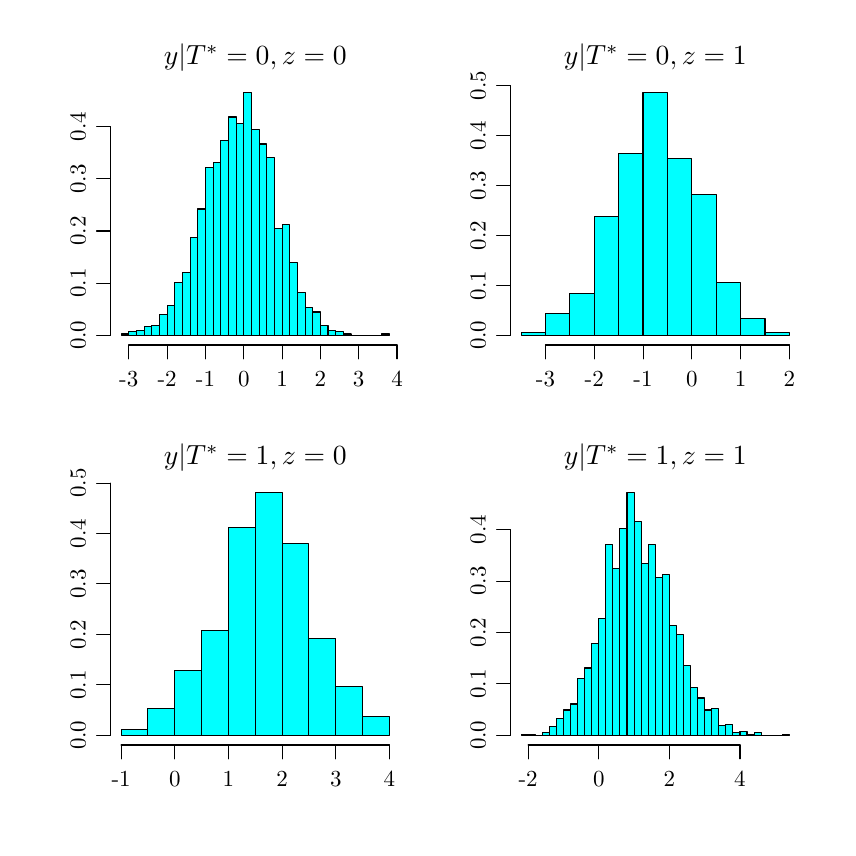
\begin{tikzpicture}[x=1pt,y=1pt]
\definecolor{fillColor}{RGB}{255,255,255}
\path[use as bounding box,fill=fillColor,fill opacity=0.00] (0,0) rectangle (289.08,289.08);
\begin{scope}
\path[clip] (  0.00,  0.00) rectangle (289.08,289.08);
\definecolor{drawColor}{RGB}{0,0,0}

\path[draw=drawColor,line width= 0.4pt,line join=round,line cap=round] ( 36.53,174.42) -- (133.47,174.42);

\path[draw=drawColor,line width= 0.4pt,line join=round,line cap=round] ( 36.53,174.42) -- ( 36.53,169.44);

\path[draw=drawColor,line width= 0.4pt,line join=round,line cap=round] ( 50.38,174.42) -- ( 50.38,169.44);

\path[draw=drawColor,line width= 0.4pt,line join=round,line cap=round] ( 64.23,174.42) -- ( 64.23,169.44);

\path[draw=drawColor,line width= 0.4pt,line join=round,line cap=round] ( 78.08,174.42) -- ( 78.08,169.44);

\path[draw=drawColor,line width= 0.4pt,line join=round,line cap=round] ( 91.93,174.42) -- ( 91.93,169.44);

\path[draw=drawColor,line width= 0.4pt,line join=round,line cap=round] (105.78,174.42) -- (105.78,169.44);

\path[draw=drawColor,line width= 0.4pt,line join=round,line cap=round] (119.63,174.42) -- (119.63,169.44);

\path[draw=drawColor,line width= 0.4pt,line join=round,line cap=round] (133.47,174.42) -- (133.47,169.44);

\node[text=drawColor,anchor=base,inner sep=0pt, outer sep=0pt, scale=  0.83] at ( 36.53,159.48) {-3};

\node[text=drawColor,anchor=base,inner sep=0pt, outer sep=0pt, scale=  0.83] at ( 50.38,159.48) {-2};

\node[text=drawColor,anchor=base,inner sep=0pt, outer sep=0pt, scale=  0.83] at ( 64.23,159.48) {-1};

\node[text=drawColor,anchor=base,inner sep=0pt, outer sep=0pt, scale=  0.83] at ( 78.08,159.48) {0};

\node[text=drawColor,anchor=base,inner sep=0pt, outer sep=0pt, scale=  0.83] at ( 91.93,159.48) {1};

\node[text=drawColor,anchor=base,inner sep=0pt, outer sep=0pt, scale=  0.83] at (105.78,159.48) {2};

\node[text=drawColor,anchor=base,inner sep=0pt, outer sep=0pt, scale=  0.83] at (119.63,159.48) {3};

\node[text=drawColor,anchor=base,inner sep=0pt, outer sep=0pt, scale=  0.83] at (133.47,159.48) {4};

\path[draw=drawColor,line width= 0.4pt,line join=round,line cap=round] ( 29.88,177.93) -- ( 29.88,253.28);

\path[draw=drawColor,line width= 0.4pt,line join=round,line cap=round] ( 29.88,177.93) -- ( 24.90,177.93);

\path[draw=drawColor,line width= 0.4pt,line join=round,line cap=round] ( 29.88,196.77) -- ( 24.90,196.77);

\path[draw=drawColor,line width= 0.4pt,line join=round,line cap=round] ( 29.88,215.61) -- ( 24.90,215.61);

\path[draw=drawColor,line width= 0.4pt,line join=round,line cap=round] ( 29.88,234.44) -- ( 24.90,234.44);

\path[draw=drawColor,line width= 0.4pt,line join=round,line cap=round] ( 29.88,253.28) -- ( 24.90,253.28);

\node[text=drawColor,rotate= 90.00,anchor=base,inner sep=0pt, outer sep=0pt, scale=  0.83] at ( 20.92,177.93) {0.0};

\node[text=drawColor,rotate= 90.00,anchor=base,inner sep=0pt, outer sep=0pt, scale=  0.83] at ( 20.92,196.77) {0.1};

\node[text=drawColor,rotate= 90.00,anchor=base,inner sep=0pt, outer sep=0pt, scale=  0.83] at ( 20.92,215.61) {0.2};

\node[text=drawColor,rotate= 90.00,anchor=base,inner sep=0pt, outer sep=0pt, scale=  0.83] at ( 20.92,234.44) {0.3};

\node[text=drawColor,rotate= 90.00,anchor=base,inner sep=0pt, outer sep=0pt, scale=  0.83] at ( 20.92,253.28) {0.4};
\end{scope}
\begin{scope}
\path[clip] (  0.00,144.54) rectangle (144.54,289.08);
\definecolor{drawColor}{RGB}{0,0,0}

\node[text=drawColor,anchor=base,inner sep=0pt, outer sep=0pt, scale=  1.00] at ( 82.23,275.68) {\bfseries $y|T^*=0,z=0$};
\end{scope}
\begin{scope}
\path[clip] ( 29.88,174.42) rectangle (134.58,269.16);
\definecolor{drawColor}{RGB}{0,0,0}
\definecolor{fillColor}{RGB}{0,255,255}

\path[draw=drawColor,line width= 0.4pt,line join=round,line cap=round,fill=fillColor] ( 33.76,177.93) rectangle ( 36.53,178.37);

\path[draw=drawColor,line width= 0.4pt,line join=round,line cap=round,fill=fillColor] ( 36.53,177.93) rectangle ( 39.30,179.26);

\path[draw=drawColor,line width= 0.4pt,line join=round,line cap=round,fill=fillColor] ( 39.30,177.93) rectangle ( 42.07,179.70);

\path[draw=drawColor,line width= 0.4pt,line join=round,line cap=round,fill=fillColor] ( 42.07,177.93) rectangle ( 44.84,181.03);

\path[draw=drawColor,line width= 0.4pt,line join=round,line cap=round,fill=fillColor] ( 44.84,177.93) rectangle ( 47.61,181.47);

\path[draw=drawColor,line width= 0.4pt,line join=round,line cap=round,fill=fillColor] ( 47.61,177.93) rectangle ( 50.38,185.46);

\path[draw=drawColor,line width= 0.4pt,line join=round,line cap=round,fill=fillColor] ( 50.38,177.93) rectangle ( 53.15,188.56);

\path[draw=drawColor,line width= 0.4pt,line join=round,line cap=round,fill=fillColor] ( 53.15,177.93) rectangle ( 55.92,196.98);

\path[draw=drawColor,line width= 0.4pt,line join=round,line cap=round,fill=fillColor] ( 55.92,177.93) rectangle ( 58.69,200.52);

\path[draw=drawColor,line width= 0.4pt,line join=round,line cap=round,fill=fillColor] ( 58.69,177.93) rectangle ( 61.46,213.37);

\path[draw=drawColor,line width= 0.4pt,line join=round,line cap=round,fill=fillColor] ( 61.46,177.93) rectangle ( 64.23,223.56);

\path[draw=drawColor,line width= 0.4pt,line join=round,line cap=round,fill=fillColor] ( 64.23,177.93) rectangle ( 67.00,238.63);

\path[draw=drawColor,line width= 0.4pt,line join=round,line cap=round,fill=fillColor] ( 67.00,177.93) rectangle ( 69.77,240.40);

\path[draw=drawColor,line width= 0.4pt,line join=round,line cap=round,fill=fillColor] ( 69.77,177.93) rectangle ( 72.54,248.37);

\path[draw=drawColor,line width= 0.4pt,line join=round,line cap=round,fill=fillColor] ( 72.54,177.93) rectangle ( 75.31,256.79);

\path[draw=drawColor,line width= 0.4pt,line join=round,line cap=round,fill=fillColor] ( 75.31,177.93) rectangle ( 78.08,254.58);

\path[draw=drawColor,line width= 0.4pt,line join=round,line cap=round,fill=fillColor] ( 78.08,177.93) rectangle ( 80.85,265.65);

\path[draw=drawColor,line width= 0.4pt,line join=round,line cap=round,fill=fillColor] ( 80.85,177.93) rectangle ( 83.61,252.36);

\path[draw=drawColor,line width= 0.4pt,line join=round,line cap=round,fill=fillColor] ( 83.61,177.93) rectangle ( 86.38,247.04);

\path[draw=drawColor,line width= 0.4pt,line join=round,line cap=round,fill=fillColor] ( 86.38,177.93) rectangle ( 89.15,242.17);

\path[draw=drawColor,line width= 0.4pt,line join=round,line cap=round,fill=fillColor] ( 89.15,177.93) rectangle ( 91.92,216.47);

\path[draw=drawColor,line width= 0.4pt,line join=round,line cap=round,fill=fillColor] ( 91.92,177.93) rectangle ( 94.69,217.80);

\path[draw=drawColor,line width= 0.4pt,line join=round,line cap=round,fill=fillColor] ( 94.69,177.93) rectangle ( 97.46,204.07);

\path[draw=drawColor,line width= 0.4pt,line join=round,line cap=round,fill=fillColor] ( 97.46,177.93) rectangle (100.23,193.44);

\path[draw=drawColor,line width= 0.4pt,line join=round,line cap=round,fill=fillColor] (100.23,177.93) rectangle (103.00,188.12);

\path[draw=drawColor,line width= 0.4pt,line join=round,line cap=round,fill=fillColor] (103.00,177.93) rectangle (105.77,186.35);

\path[draw=drawColor,line width= 0.4pt,line join=round,line cap=round,fill=fillColor] (105.77,177.93) rectangle (108.54,181.47);

\path[draw=drawColor,line width= 0.4pt,line join=round,line cap=round,fill=fillColor] (108.54,177.93) rectangle (111.31,179.70);

\path[draw=drawColor,line width= 0.4pt,line join=round,line cap=round,fill=fillColor] (111.31,177.93) rectangle (114.08,179.26);

\path[draw=drawColor,line width= 0.4pt,line join=round,line cap=round,fill=fillColor] (114.08,177.93) rectangle (116.85,178.37);

\path[draw=drawColor,line width= 0.4pt,line join=round,line cap=round,fill=fillColor] (116.85,177.93) rectangle (119.62,177.93);

\path[draw=drawColor,line width= 0.4pt,line join=round,line cap=round,fill=fillColor] (119.62,177.93) rectangle (122.39,177.93);

\path[draw=drawColor,line width= 0.4pt,line join=round,line cap=round,fill=fillColor] (122.39,177.93) rectangle (125.16,177.93);

\path[draw=drawColor,line width= 0.4pt,line join=round,line cap=round,fill=fillColor] (125.16,177.93) rectangle (127.93,177.93);

\path[draw=drawColor,line width= 0.4pt,line join=round,line cap=round,fill=fillColor] (127.93,177.93) rectangle (130.70,178.37);
\end{scope}
\begin{scope}
\path[clip] (  0.00,  0.00) rectangle (289.08,289.08);
\definecolor{drawColor}{RGB}{0,0,0}

\path[draw=drawColor,line width= 0.4pt,line join=round,line cap=round] (187.12,174.42) -- (275.25,174.42);

\path[draw=drawColor,line width= 0.4pt,line join=round,line cap=round] (187.12,174.42) -- (187.12,169.44);

\path[draw=drawColor,line width= 0.4pt,line join=round,line cap=round] (204.75,174.42) -- (204.75,169.44);

\path[draw=drawColor,line width= 0.4pt,line join=round,line cap=round] (222.37,174.42) -- (222.37,169.44);

\path[draw=drawColor,line width= 0.4pt,line join=round,line cap=round] (240.00,174.42) -- (240.00,169.44);

\path[draw=drawColor,line width= 0.4pt,line join=round,line cap=round] (257.62,174.42) -- (257.62,169.44);

\path[draw=drawColor,line width= 0.4pt,line join=round,line cap=round] (275.25,174.42) -- (275.25,169.44);

\node[text=drawColor,anchor=base,inner sep=0pt, outer sep=0pt, scale=  0.83] at (187.12,159.48) {-3};

\node[text=drawColor,anchor=base,inner sep=0pt, outer sep=0pt, scale=  0.83] at (204.75,159.48) {-2};

\node[text=drawColor,anchor=base,inner sep=0pt, outer sep=0pt, scale=  0.83] at (222.37,159.48) {-1};

\node[text=drawColor,anchor=base,inner sep=0pt, outer sep=0pt, scale=  0.83] at (240.00,159.48) {0};

\node[text=drawColor,anchor=base,inner sep=0pt, outer sep=0pt, scale=  0.83] at (257.62,159.48) {1};

\node[text=drawColor,anchor=base,inner sep=0pt, outer sep=0pt, scale=  0.83] at (275.25,159.48) {2};

\path[draw=drawColor,line width= 0.4pt,line join=round,line cap=round] (174.42,177.93) -- (174.42,268.14);

\path[draw=drawColor,line width= 0.4pt,line join=round,line cap=round] (174.42,177.93) -- (169.44,177.93);

\path[draw=drawColor,line width= 0.4pt,line join=round,line cap=round] (174.42,195.97) -- (169.44,195.97);

\path[draw=drawColor,line width= 0.4pt,line join=round,line cap=round] (174.42,214.01) -- (169.44,214.01);

\path[draw=drawColor,line width= 0.4pt,line join=round,line cap=round] (174.42,232.06) -- (169.44,232.06);

\path[draw=drawColor,line width= 0.4pt,line join=round,line cap=round] (174.42,250.10) -- (169.44,250.10);

\path[draw=drawColor,line width= 0.4pt,line join=round,line cap=round] (174.42,268.14) -- (169.44,268.14);

\node[text=drawColor,rotate= 90.00,anchor=base,inner sep=0pt, outer sep=0pt, scale=  0.83] at (165.46,177.93) {0.0};

\node[text=drawColor,rotate= 90.00,anchor=base,inner sep=0pt, outer sep=0pt, scale=  0.83] at (165.46,195.97) {0.1};

\node[text=drawColor,rotate= 90.00,anchor=base,inner sep=0pt, outer sep=0pt, scale=  0.83] at (165.46,214.01) {0.2};

\node[text=drawColor,rotate= 90.00,anchor=base,inner sep=0pt, outer sep=0pt, scale=  0.83] at (165.46,232.06) {0.3};

\node[text=drawColor,rotate= 90.00,anchor=base,inner sep=0pt, outer sep=0pt, scale=  0.83] at (165.46,250.10) {0.4};

\node[text=drawColor,rotate= 90.00,anchor=base,inner sep=0pt, outer sep=0pt, scale=  0.83] at (165.46,268.14) {0.5};
\end{scope}
\begin{scope}
\path[clip] (144.54,144.54) rectangle (289.08,289.08);
\definecolor{drawColor}{RGB}{0,0,0}

\node[text=drawColor,anchor=base,inner sep=0pt, outer sep=0pt, scale=  1.00] at (226.77,275.68) {\bfseries $y|T^*=0,z=1$};
\end{scope}
\begin{scope}
\path[clip] (174.42,174.42) rectangle (279.12,269.16);
\definecolor{drawColor}{RGB}{0,0,0}
\definecolor{fillColor}{RGB}{0,255,255}

\path[draw=drawColor,line width= 0.4pt,line join=round,line cap=round,fill=fillColor] (178.30,177.93) rectangle (187.11,178.93);

\path[draw=drawColor,line width= 0.4pt,line join=round,line cap=round,fill=fillColor] (187.11,177.93) rectangle (195.92,185.90);

\path[draw=drawColor,line width= 0.4pt,line join=round,line cap=round,fill=fillColor] (195.92,177.93) rectangle (204.74,192.88);

\path[draw=drawColor,line width= 0.4pt,line join=round,line cap=round,fill=fillColor] (204.74,177.93) rectangle (213.55,220.79);

\path[draw=drawColor,line width= 0.4pt,line join=round,line cap=round,fill=fillColor] (213.55,177.93) rectangle (222.36,243.72);

\path[draw=drawColor,line width= 0.4pt,line join=round,line cap=round,fill=fillColor] (222.36,177.93) rectangle (231.18,265.65);

\path[draw=drawColor,line width= 0.4pt,line join=round,line cap=round,fill=fillColor] (231.18,177.93) rectangle (239.99,241.73);

\path[draw=drawColor,line width= 0.4pt,line join=round,line cap=round,fill=fillColor] (239.99,177.93) rectangle (248.80,228.77);

\path[draw=drawColor,line width= 0.4pt,line join=round,line cap=round,fill=fillColor] (248.80,177.93) rectangle (257.62,196.87);

\path[draw=drawColor,line width= 0.4pt,line join=round,line cap=round,fill=fillColor] (257.62,177.93) rectangle (266.43,183.91);

\path[draw=drawColor,line width= 0.4pt,line join=round,line cap=round,fill=fillColor] (266.43,177.93) rectangle (275.24,178.93);
\end{scope}
\begin{scope}
\path[clip] (  0.00,  0.00) rectangle (289.08,289.08);
\definecolor{drawColor}{RGB}{0,0,0}

\path[draw=drawColor,line width= 0.4pt,line join=round,line cap=round] ( 33.77, 29.88) -- (130.71, 29.88);

\path[draw=drawColor,line width= 0.4pt,line join=round,line cap=round] ( 33.77, 29.88) -- ( 33.77, 24.90);

\path[draw=drawColor,line width= 0.4pt,line join=round,line cap=round] ( 53.16, 29.88) -- ( 53.16, 24.90);

\path[draw=drawColor,line width= 0.4pt,line join=round,line cap=round] ( 72.55, 29.88) -- ( 72.55, 24.90);

\path[draw=drawColor,line width= 0.4pt,line join=round,line cap=round] ( 91.93, 29.88) -- ( 91.93, 24.90);

\path[draw=drawColor,line width= 0.4pt,line join=round,line cap=round] (111.32, 29.88) -- (111.32, 24.90);

\path[draw=drawColor,line width= 0.4pt,line join=round,line cap=round] (130.71, 29.88) -- (130.71, 24.90);

\node[text=drawColor,anchor=base,inner sep=0pt, outer sep=0pt, scale=  0.83] at ( 33.77, 14.94) {-1};

\node[text=drawColor,anchor=base,inner sep=0pt, outer sep=0pt, scale=  0.83] at ( 53.16, 14.94) {0};

\node[text=drawColor,anchor=base,inner sep=0pt, outer sep=0pt, scale=  0.83] at ( 72.55, 14.94) {1};

\node[text=drawColor,anchor=base,inner sep=0pt, outer sep=0pt, scale=  0.83] at ( 91.93, 14.94) {2};

\node[text=drawColor,anchor=base,inner sep=0pt, outer sep=0pt, scale=  0.83] at (111.32, 14.94) {3};

\node[text=drawColor,anchor=base,inner sep=0pt, outer sep=0pt, scale=  0.83] at (130.71, 14.94) {4};

\path[draw=drawColor,line width= 0.4pt,line join=round,line cap=round] ( 29.88, 33.39) -- ( 29.88,124.52);

\path[draw=drawColor,line width= 0.4pt,line join=round,line cap=round] ( 29.88, 33.39) -- ( 24.90, 33.39);

\path[draw=drawColor,line width= 0.4pt,line join=round,line cap=round] ( 29.88, 51.62) -- ( 24.90, 51.62);

\path[draw=drawColor,line width= 0.4pt,line join=round,line cap=round] ( 29.88, 69.84) -- ( 24.90, 69.84);

\path[draw=drawColor,line width= 0.4pt,line join=round,line cap=round] ( 29.88, 88.07) -- ( 24.90, 88.07);

\path[draw=drawColor,line width= 0.4pt,line join=round,line cap=round] ( 29.88,106.30) -- ( 24.90,106.30);

\path[draw=drawColor,line width= 0.4pt,line join=round,line cap=round] ( 29.88,124.52) -- ( 24.90,124.52);

\node[text=drawColor,rotate= 90.00,anchor=base,inner sep=0pt, outer sep=0pt, scale=  0.83] at ( 20.92, 33.39) {0.0};

\node[text=drawColor,rotate= 90.00,anchor=base,inner sep=0pt, outer sep=0pt, scale=  0.83] at ( 20.92, 51.62) {0.1};

\node[text=drawColor,rotate= 90.00,anchor=base,inner sep=0pt, outer sep=0pt, scale=  0.83] at ( 20.92, 69.84) {0.2};

\node[text=drawColor,rotate= 90.00,anchor=base,inner sep=0pt, outer sep=0pt, scale=  0.83] at ( 20.92, 88.07) {0.3};

\node[text=drawColor,rotate= 90.00,anchor=base,inner sep=0pt, outer sep=0pt, scale=  0.83] at ( 20.92,106.30) {0.4};

\node[text=drawColor,rotate= 90.00,anchor=base,inner sep=0pt, outer sep=0pt, scale=  0.83] at ( 20.92,124.52) {0.5};
\end{scope}
\begin{scope}
\path[clip] (  0.00,  0.00) rectangle (144.54,144.54);
\definecolor{drawColor}{RGB}{0,0,0}

\node[text=drawColor,anchor=base,inner sep=0pt, outer sep=0pt, scale=  1.00] at ( 82.23,131.14) {\bfseries $y|T^*=1,z=0$};
\end{scope}
\begin{scope}
\path[clip] ( 29.88, 29.88) rectangle (134.58,124.62);
\definecolor{drawColor}{RGB}{0,0,0}
\definecolor{fillColor}{RGB}{0,255,255}

\path[draw=drawColor,line width= 0.4pt,line join=round,line cap=round,fill=fillColor] ( 33.76, 33.39) rectangle ( 43.45, 35.34);

\path[draw=drawColor,line width= 0.4pt,line join=round,line cap=round,fill=fillColor] ( 43.45, 33.39) rectangle ( 53.15, 43.14);

\path[draw=drawColor,line width= 0.4pt,line join=round,line cap=round,fill=fillColor] ( 53.15, 33.39) rectangle ( 62.84, 56.78);

\path[draw=drawColor,line width= 0.4pt,line join=round,line cap=round,fill=fillColor] ( 62.84, 33.39) rectangle ( 72.54, 71.40);

\path[draw=drawColor,line width= 0.4pt,line join=round,line cap=round,fill=fillColor] ( 72.54, 33.39) rectangle ( 82.23,108.44);

\path[draw=drawColor,line width= 0.4pt,line join=round,line cap=round,fill=fillColor] ( 82.23, 33.39) rectangle ( 91.92,121.11);

\path[draw=drawColor,line width= 0.4pt,line join=round,line cap=round,fill=fillColor] ( 91.92, 33.39) rectangle (101.62,102.59);

\path[draw=drawColor,line width= 0.4pt,line join=round,line cap=round,fill=fillColor] (101.62, 33.39) rectangle (111.31, 68.48);

\path[draw=drawColor,line width= 0.4pt,line join=round,line cap=round,fill=fillColor] (111.31, 33.39) rectangle (121.01, 50.93);

\path[draw=drawColor,line width= 0.4pt,line join=round,line cap=round,fill=fillColor] (121.01, 33.39) rectangle (130.70, 40.21);
\end{scope}
\begin{scope}
\path[clip] (  0.00,  0.00) rectangle (289.08,289.08);
\definecolor{drawColor}{RGB}{0,0,0}

\path[draw=drawColor,line width= 0.4pt,line join=round,line cap=round] (180.85, 29.88) -- (257.39, 29.88);

\path[draw=drawColor,line width= 0.4pt,line join=round,line cap=round] (180.85, 29.88) -- (180.85, 24.90);

\path[draw=drawColor,line width= 0.4pt,line join=round,line cap=round] (206.36, 29.88) -- (206.36, 24.90);

\path[draw=drawColor,line width= 0.4pt,line join=round,line cap=round] (231.87, 29.88) -- (231.87, 24.90);

\path[draw=drawColor,line width= 0.4pt,line join=round,line cap=round] (257.39, 29.88) -- (257.39, 24.90);

\node[text=drawColor,anchor=base,inner sep=0pt, outer sep=0pt, scale=  0.83] at (180.85, 14.94) {-2};

\node[text=drawColor,anchor=base,inner sep=0pt, outer sep=0pt, scale=  0.83] at (206.36, 14.94) {0};

\node[text=drawColor,anchor=base,inner sep=0pt, outer sep=0pt, scale=  0.83] at (231.87, 14.94) {2};

\node[text=drawColor,anchor=base,inner sep=0pt, outer sep=0pt, scale=  0.83] at (257.39, 14.94) {4};

\path[draw=drawColor,line width= 0.4pt,line join=round,line cap=round] (174.42, 33.39) -- (174.42,107.67);

\path[draw=drawColor,line width= 0.4pt,line join=round,line cap=round] (174.42, 33.39) -- (169.44, 33.39);

\path[draw=drawColor,line width= 0.4pt,line join=round,line cap=round] (174.42, 51.96) -- (169.44, 51.96);

\path[draw=drawColor,line width= 0.4pt,line join=round,line cap=round] (174.42, 70.53) -- (169.44, 70.53);

\path[draw=drawColor,line width= 0.4pt,line join=round,line cap=round] (174.42, 89.10) -- (169.44, 89.10);

\path[draw=drawColor,line width= 0.4pt,line join=round,line cap=round] (174.42,107.67) -- (169.44,107.67);

\node[text=drawColor,rotate= 90.00,anchor=base,inner sep=0pt, outer sep=0pt, scale=  0.83] at (165.46, 33.39) {0.0};

\node[text=drawColor,rotate= 90.00,anchor=base,inner sep=0pt, outer sep=0pt, scale=  0.83] at (165.46, 51.96) {0.1};

\node[text=drawColor,rotate= 90.00,anchor=base,inner sep=0pt, outer sep=0pt, scale=  0.83] at (165.46, 70.53) {0.2};

\node[text=drawColor,rotate= 90.00,anchor=base,inner sep=0pt, outer sep=0pt, scale=  0.83] at (165.46, 89.10) {0.3};

\node[text=drawColor,rotate= 90.00,anchor=base,inner sep=0pt, outer sep=0pt, scale=  0.83] at (165.46,107.67) {0.4};
\end{scope}
\begin{scope}
\path[clip] (144.54,  0.00) rectangle (289.08,144.54);
\definecolor{drawColor}{RGB}{0,0,0}

\node[text=drawColor,anchor=base,inner sep=0pt, outer sep=0pt, scale=  1.00] at (226.77,131.14) {\bfseries $y|T^*=1,z=1$};
\end{scope}
\begin{scope}
\path[clip] (174.42, 29.88) rectangle (279.12,124.62);
\definecolor{drawColor}{RGB}{0,0,0}
\definecolor{fillColor}{RGB}{0,255,255}

\path[draw=drawColor,line width= 0.4pt,line join=round,line cap=round,fill=fillColor] (178.30, 33.39) rectangle (180.85, 33.82);

\path[draw=drawColor,line width= 0.4pt,line join=round,line cap=round,fill=fillColor] (180.85, 33.39) rectangle (183.40, 33.82);

\path[draw=drawColor,line width= 0.4pt,line join=round,line cap=round,fill=fillColor] (183.40, 33.39) rectangle (185.95, 33.39);

\path[draw=drawColor,line width= 0.4pt,line join=round,line cap=round,fill=fillColor] (185.95, 33.39) rectangle (188.50, 34.26);

\path[draw=drawColor,line width= 0.4pt,line join=round,line cap=round,fill=fillColor] (188.50, 33.39) rectangle (191.05, 36.43);

\path[draw=drawColor,line width= 0.4pt,line join=round,line cap=round,fill=fillColor] (191.05, 33.39) rectangle (193.60, 39.47);

\path[draw=drawColor,line width= 0.4pt,line join=round,line cap=round,fill=fillColor] (193.60, 33.39) rectangle (196.16, 42.51);

\path[draw=drawColor,line width= 0.4pt,line join=round,line cap=round,fill=fillColor] (196.16, 33.39) rectangle (198.71, 44.68);

\path[draw=drawColor,line width= 0.4pt,line join=round,line cap=round,fill=fillColor] (198.71, 33.39) rectangle (201.26, 53.80);

\path[draw=drawColor,line width= 0.4pt,line join=round,line cap=round,fill=fillColor] (201.26, 33.39) rectangle (203.81, 57.71);

\path[draw=drawColor,line width= 0.4pt,line join=round,line cap=round,fill=fillColor] (203.81, 33.39) rectangle (206.36, 66.39);

\path[draw=drawColor,line width= 0.4pt,line join=round,line cap=round,fill=fillColor] (206.36, 33.39) rectangle (208.91, 75.51);

\path[draw=drawColor,line width= 0.4pt,line join=round,line cap=round,fill=fillColor] (208.91, 33.39) rectangle (211.46,102.44);

\path[draw=drawColor,line width= 0.4pt,line join=round,line cap=round,fill=fillColor] (211.46, 33.39) rectangle (214.01, 93.75);

\path[draw=drawColor,line width= 0.4pt,line join=round,line cap=round,fill=fillColor] (214.01, 33.39) rectangle (216.57,108.08);

\path[draw=drawColor,line width= 0.4pt,line join=round,line cap=round,fill=fillColor] (216.57, 33.39) rectangle (219.12,121.11);

\path[draw=drawColor,line width= 0.4pt,line join=round,line cap=round,fill=fillColor] (219.12, 33.39) rectangle (221.67,110.69);

\path[draw=drawColor,line width= 0.4pt,line join=round,line cap=round,fill=fillColor] (221.67, 33.39) rectangle (224.22, 95.49);

\path[draw=drawColor,line width= 0.4pt,line join=round,line cap=round,fill=fillColor] (224.22, 33.39) rectangle (226.77,102.44);

\path[draw=drawColor,line width= 0.4pt,line join=round,line cap=round,fill=fillColor] (226.77, 33.39) rectangle (229.32, 90.28);

\path[draw=drawColor,line width= 0.4pt,line join=round,line cap=round,fill=fillColor] (229.32, 33.39) rectangle (231.87, 91.58);

\path[draw=drawColor,line width= 0.4pt,line join=round,line cap=round,fill=fillColor] (231.87, 33.39) rectangle (234.42, 72.91);

\path[draw=drawColor,line width= 0.4pt,line join=round,line cap=round,fill=fillColor] (234.42, 33.39) rectangle (236.97, 69.87);

\path[draw=drawColor,line width= 0.4pt,line join=round,line cap=round,fill=fillColor] (236.97, 33.39) rectangle (239.53, 58.58);

\path[draw=drawColor,line width= 0.4pt,line join=round,line cap=round,fill=fillColor] (239.53, 33.39) rectangle (242.08, 50.76);

\path[draw=drawColor,line width= 0.4pt,line join=round,line cap=round,fill=fillColor] (242.08, 33.39) rectangle (244.63, 46.85);

\path[draw=drawColor,line width= 0.4pt,line join=round,line cap=round,fill=fillColor] (244.63, 33.39) rectangle (247.18, 42.51);

\path[draw=drawColor,line width= 0.4pt,line join=round,line cap=round,fill=fillColor] (247.18, 33.39) rectangle (249.73, 42.94);

\path[draw=drawColor,line width= 0.4pt,line join=round,line cap=round,fill=fillColor] (249.73, 33.39) rectangle (252.28, 36.86);

\path[draw=drawColor,line width= 0.4pt,line join=round,line cap=round,fill=fillColor] (252.28, 33.39) rectangle (254.83, 37.30);

\path[draw=drawColor,line width= 0.4pt,line join=round,line cap=round,fill=fillColor] (254.83, 33.39) rectangle (257.38, 34.26);

\path[draw=drawColor,line width= 0.4pt,line join=round,line cap=round,fill=fillColor] (257.38, 33.39) rectangle (259.94, 34.69);

\path[draw=drawColor,line width= 0.4pt,line join=round,line cap=round,fill=fillColor] (259.94, 33.39) rectangle (262.49, 33.82);

\path[draw=drawColor,line width= 0.4pt,line join=round,line cap=round,fill=fillColor] (262.49, 33.39) rectangle (265.04, 34.26);

\path[draw=drawColor,line width= 0.4pt,line join=round,line cap=round,fill=fillColor] (265.04, 33.39) rectangle (267.59, 33.39);

\path[draw=drawColor,line width= 0.4pt,line join=round,line cap=round,fill=fillColor] (267.59, 33.39) rectangle (270.14, 33.39);

\path[draw=drawColor,line width= 0.4pt,line join=round,line cap=round,fill=fillColor] (270.14, 33.39) rectangle (272.69, 33.39);

\path[draw=drawColor,line width= 0.4pt,line join=round,line cap=round,fill=fillColor] (272.69, 33.39) rectangle (275.24, 33.82);
\end{scope}
\end{tikzpicture}

%}
%\end{figure}
%\[\widehat{\beta}_{IV} = 0.96, \quad \mbox{95\% CI } = (0.88, 1.04)\]
%\end{block}
%\end{frame}
%%%%%%%%%%%%%%%%%%%%%%%%%%%%%%%%%%%%%%
%\begin{frame}[noframenumbering]
%  \frametitle{Example \hfill \small{(sim data: $\beta = 1, \alpha_0 = 0.1, \alpha_1 = 0.2, n = 5000$)}}
%
%  \begin{alertblock}{Results using $T$ instead of $T^*$}
%\begin{figure}[h]
%  \centering
%\resizebox{0.5\textwidth}{!}{%
%  % Created by tikzDevice version 0.10.1 on 2018-01-16 22:08:40
% !TEX encoding = UTF-8 Unicode
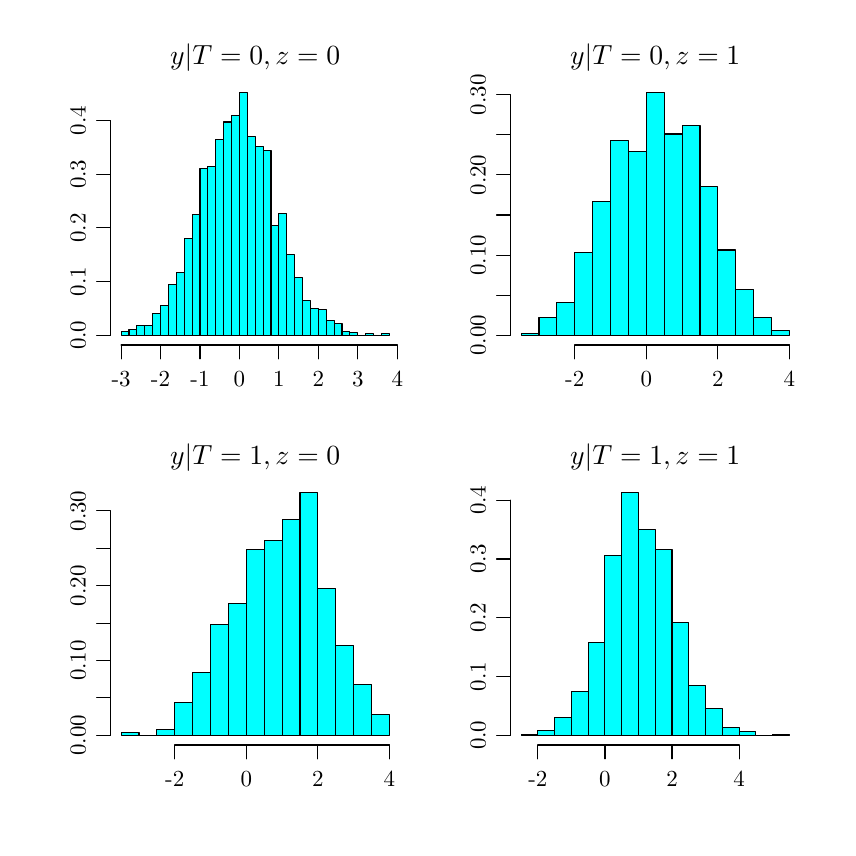
\begin{tikzpicture}[x=1pt,y=1pt]
\definecolor{fillColor}{RGB}{255,255,255}
\path[use as bounding box,fill=fillColor,fill opacity=0.00] (0,0) rectangle (289.08,289.08);
\begin{scope}
\path[clip] (  0.00,  0.00) rectangle (289.08,289.08);
\definecolor{drawColor}{RGB}{0,0,0}

\path[draw=drawColor,line width= 0.4pt,line join=round,line cap=round] ( 33.76,174.42) -- (133.56,174.42);

\path[draw=drawColor,line width= 0.4pt,line join=round,line cap=round] ( 33.76,174.42) -- ( 33.76,169.44);

\path[draw=drawColor,line width= 0.4pt,line join=round,line cap=round] ( 48.02,174.42) -- ( 48.02,169.44);

\path[draw=drawColor,line width= 0.4pt,line join=round,line cap=round] ( 62.27,174.42) -- ( 62.27,169.44);

\path[draw=drawColor,line width= 0.4pt,line join=round,line cap=round] ( 76.53,174.42) -- ( 76.53,169.44);

\path[draw=drawColor,line width= 0.4pt,line join=round,line cap=round] ( 90.79,174.42) -- ( 90.79,169.44);

\path[draw=drawColor,line width= 0.4pt,line join=round,line cap=round] (105.04,174.42) -- (105.04,169.44);

\path[draw=drawColor,line width= 0.4pt,line join=round,line cap=round] (119.30,174.42) -- (119.30,169.44);

\path[draw=drawColor,line width= 0.4pt,line join=round,line cap=round] (133.56,174.42) -- (133.56,169.44);

\node[text=drawColor,anchor=base,inner sep=0pt, outer sep=0pt, scale=  0.83] at ( 33.76,159.48) {-3};

\node[text=drawColor,anchor=base,inner sep=0pt, outer sep=0pt, scale=  0.83] at ( 48.02,159.48) {-2};

\node[text=drawColor,anchor=base,inner sep=0pt, outer sep=0pt, scale=  0.83] at ( 62.27,159.48) {-1};

\node[text=drawColor,anchor=base,inner sep=0pt, outer sep=0pt, scale=  0.83] at ( 76.53,159.48) {0};

\node[text=drawColor,anchor=base,inner sep=0pt, outer sep=0pt, scale=  0.83] at ( 90.79,159.48) {1};

\node[text=drawColor,anchor=base,inner sep=0pt, outer sep=0pt, scale=  0.83] at (105.04,159.48) {2};

\node[text=drawColor,anchor=base,inner sep=0pt, outer sep=0pt, scale=  0.83] at (119.30,159.48) {3};

\node[text=drawColor,anchor=base,inner sep=0pt, outer sep=0pt, scale=  0.83] at (133.56,159.48) {4};

\path[draw=drawColor,line width= 0.4pt,line join=round,line cap=round] ( 29.88,177.93) -- ( 29.88,255.51);

\path[draw=drawColor,line width= 0.4pt,line join=round,line cap=round] ( 29.88,177.93) -- ( 24.90,177.93);

\path[draw=drawColor,line width= 0.4pt,line join=round,line cap=round] ( 29.88,197.32) -- ( 24.90,197.32);

\path[draw=drawColor,line width= 0.4pt,line join=round,line cap=round] ( 29.88,216.72) -- ( 24.90,216.72);

\path[draw=drawColor,line width= 0.4pt,line join=round,line cap=round] ( 29.88,236.12) -- ( 24.90,236.12);

\path[draw=drawColor,line width= 0.4pt,line join=round,line cap=round] ( 29.88,255.51) -- ( 24.90,255.51);

\node[text=drawColor,rotate= 90.00,anchor=base,inner sep=0pt, outer sep=0pt, scale=  0.83] at ( 20.92,177.93) {0.0};

\node[text=drawColor,rotate= 90.00,anchor=base,inner sep=0pt, outer sep=0pt, scale=  0.83] at ( 20.92,197.32) {0.1};

\node[text=drawColor,rotate= 90.00,anchor=base,inner sep=0pt, outer sep=0pt, scale=  0.83] at ( 20.92,216.72) {0.2};

\node[text=drawColor,rotate= 90.00,anchor=base,inner sep=0pt, outer sep=0pt, scale=  0.83] at ( 20.92,236.12) {0.3};

\node[text=drawColor,rotate= 90.00,anchor=base,inner sep=0pt, outer sep=0pt, scale=  0.83] at ( 20.92,255.51) {0.4};
\end{scope}
\begin{scope}
\path[clip] (  0.00,144.54) rectangle (144.54,289.08);
\definecolor{drawColor}{RGB}{0,0,0}

\node[text=drawColor,anchor=base,inner sep=0pt, outer sep=0pt, scale=  1.00] at ( 82.23,275.68) {\bfseries $y|T=0,z=0$};
\end{scope}
\begin{scope}
\path[clip] ( 29.88,174.42) rectangle (134.58,269.16);
\definecolor{drawColor}{RGB}{0,0,0}
\definecolor{fillColor}{RGB}{0,255,255}

\path[draw=drawColor,line width= 0.4pt,line join=round,line cap=round,fill=fillColor] ( 33.76,177.93) rectangle ( 36.61,179.38);

\path[draw=drawColor,line width= 0.4pt,line join=round,line cap=round,fill=fillColor] ( 36.61,177.93) rectangle ( 39.46,179.87);

\path[draw=drawColor,line width= 0.4pt,line join=round,line cap=round,fill=fillColor] ( 39.46,177.93) rectangle ( 42.31,181.32);

\path[draw=drawColor,line width= 0.4pt,line join=round,line cap=round,fill=fillColor] ( 42.31,177.93) rectangle ( 45.16,181.32);

\path[draw=drawColor,line width= 0.4pt,line join=round,line cap=round,fill=fillColor] ( 45.16,177.93) rectangle ( 48.01,185.68);

\path[draw=drawColor,line width= 0.4pt,line join=round,line cap=round,fill=fillColor] ( 48.01,177.93) rectangle ( 50.87,188.59);

\path[draw=drawColor,line width= 0.4pt,line join=round,line cap=round,fill=fillColor] ( 50.87,177.93) rectangle ( 53.72,196.35);

\path[draw=drawColor,line width= 0.4pt,line join=round,line cap=round,fill=fillColor] ( 53.72,177.93) rectangle ( 56.57,200.71);

\path[draw=drawColor,line width= 0.4pt,line join=round,line cap=round,fill=fillColor] ( 56.57,177.93) rectangle ( 59.42,212.82);

\path[draw=drawColor,line width= 0.4pt,line join=round,line cap=round,fill=fillColor] ( 59.42,177.93) rectangle ( 62.27,221.55);

\path[draw=drawColor,line width= 0.4pt,line join=round,line cap=round,fill=fillColor] ( 62.27,177.93) rectangle ( 65.12,238.03);

\path[draw=drawColor,line width= 0.4pt,line join=round,line cap=round,fill=fillColor] ( 65.12,177.93) rectangle ( 67.97,239.00);

\path[draw=drawColor,line width= 0.4pt,line join=round,line cap=round,fill=fillColor] ( 67.97,177.93) rectangle ( 70.82,248.69);

\path[draw=drawColor,line width= 0.4pt,line join=round,line cap=round,fill=fillColor] ( 70.82,177.93) rectangle ( 73.68,254.99);

\path[draw=drawColor,line width= 0.4pt,line join=round,line cap=round,fill=fillColor] ( 73.68,177.93) rectangle ( 76.53,257.41);

\path[draw=drawColor,line width= 0.4pt,line join=round,line cap=round,fill=fillColor] ( 76.53,177.93) rectangle ( 79.38,265.65);

\path[draw=drawColor,line width= 0.4pt,line join=round,line cap=round,fill=fillColor] ( 79.38,177.93) rectangle ( 82.23,249.66);

\path[draw=drawColor,line width= 0.4pt,line join=round,line cap=round,fill=fillColor] ( 82.23,177.93) rectangle ( 85.08,246.26);

\path[draw=drawColor,line width= 0.4pt,line join=round,line cap=round,fill=fillColor] ( 85.08,177.93) rectangle ( 87.93,244.81);

\path[draw=drawColor,line width= 0.4pt,line join=round,line cap=round,fill=fillColor] ( 87.93,177.93) rectangle ( 90.78,217.67);

\path[draw=drawColor,line width= 0.4pt,line join=round,line cap=round,fill=fillColor] ( 90.78,177.93) rectangle ( 93.64,222.03);

\path[draw=drawColor,line width= 0.4pt,line join=round,line cap=round,fill=fillColor] ( 93.64,177.93) rectangle ( 96.49,207.01);

\path[draw=drawColor,line width= 0.4pt,line join=round,line cap=round,fill=fillColor] ( 96.49,177.93) rectangle ( 99.34,198.77);

\path[draw=drawColor,line width= 0.4pt,line join=round,line cap=round,fill=fillColor] ( 99.34,177.93) rectangle (102.19,190.53);

\path[draw=drawColor,line width= 0.4pt,line join=round,line cap=round,fill=fillColor] (102.19,177.93) rectangle (105.04,187.62);

\path[draw=drawColor,line width= 0.4pt,line join=round,line cap=round,fill=fillColor] (105.04,177.93) rectangle (107.89,187.14);

\path[draw=drawColor,line width= 0.4pt,line join=round,line cap=round,fill=fillColor] (107.89,177.93) rectangle (110.74,183.26);

\path[draw=drawColor,line width= 0.4pt,line join=round,line cap=round,fill=fillColor] (110.74,177.93) rectangle (113.59,182.29);

\path[draw=drawColor,line width= 0.4pt,line join=round,line cap=round,fill=fillColor] (113.59,177.93) rectangle (116.45,179.38);

\path[draw=drawColor,line width= 0.4pt,line join=round,line cap=round,fill=fillColor] (116.45,177.93) rectangle (119.30,178.90);

\path[draw=drawColor,line width= 0.4pt,line join=round,line cap=round,fill=fillColor] (119.30,177.93) rectangle (122.15,177.93);

\path[draw=drawColor,line width= 0.4pt,line join=round,line cap=round,fill=fillColor] (122.15,177.93) rectangle (125.00,178.41);

\path[draw=drawColor,line width= 0.4pt,line join=round,line cap=round,fill=fillColor] (125.00,177.93) rectangle (127.85,177.93);

\path[draw=drawColor,line width= 0.4pt,line join=round,line cap=round,fill=fillColor] (127.85,177.93) rectangle (130.70,178.41);
\end{scope}
\begin{scope}
\path[clip] (  0.00,  0.00) rectangle (289.08,289.08);
\definecolor{drawColor}{RGB}{0,0,0}

\path[draw=drawColor,line width= 0.4pt,line join=round,line cap=round] (197.69,174.42) -- (275.25,174.42);

\path[draw=drawColor,line width= 0.4pt,line join=round,line cap=round] (197.69,174.42) -- (197.69,169.44);

\path[draw=drawColor,line width= 0.4pt,line join=round,line cap=round] (223.54,174.42) -- (223.54,169.44);

\path[draw=drawColor,line width= 0.4pt,line join=round,line cap=round] (249.40,174.42) -- (249.40,169.44);

\path[draw=drawColor,line width= 0.4pt,line join=round,line cap=round] (275.25,174.42) -- (275.25,169.44);

\node[text=drawColor,anchor=base,inner sep=0pt, outer sep=0pt, scale=  0.83] at (197.69,159.48) {-2};

\node[text=drawColor,anchor=base,inner sep=0pt, outer sep=0pt, scale=  0.83] at (223.54,159.48) {0};

\node[text=drawColor,anchor=base,inner sep=0pt, outer sep=0pt, scale=  0.83] at (249.40,159.48) {2};

\node[text=drawColor,anchor=base,inner sep=0pt, outer sep=0pt, scale=  0.83] at (275.25,159.48) {4};

\path[draw=drawColor,line width= 0.4pt,line join=round,line cap=round] (174.42,177.93) -- (174.42,264.82);

\path[draw=drawColor,line width= 0.4pt,line join=round,line cap=round] (174.42,177.93) -- (169.44,177.93);

\path[draw=drawColor,line width= 0.4pt,line join=round,line cap=round] (174.42,192.41) -- (169.44,192.41);

\path[draw=drawColor,line width= 0.4pt,line join=round,line cap=round] (174.42,206.89) -- (169.44,206.89);

\path[draw=drawColor,line width= 0.4pt,line join=round,line cap=round] (174.42,221.38) -- (169.44,221.38);

\path[draw=drawColor,line width= 0.4pt,line join=round,line cap=round] (174.42,235.86) -- (169.44,235.86);

\path[draw=drawColor,line width= 0.4pt,line join=round,line cap=round] (174.42,250.34) -- (169.44,250.34);

\path[draw=drawColor,line width= 0.4pt,line join=round,line cap=round] (174.42,264.82) -- (169.44,264.82);

\node[text=drawColor,rotate= 90.00,anchor=base,inner sep=0pt, outer sep=0pt, scale=  0.83] at (165.46,177.93) {0.00};

\node[text=drawColor,rotate= 90.00,anchor=base,inner sep=0pt, outer sep=0pt, scale=  0.83] at (165.46,206.89) {0.10};

\node[text=drawColor,rotate= 90.00,anchor=base,inner sep=0pt, outer sep=0pt, scale=  0.83] at (165.46,235.86) {0.20};

\node[text=drawColor,rotate= 90.00,anchor=base,inner sep=0pt, outer sep=0pt, scale=  0.83] at (165.46,264.82) {0.30};
\end{scope}
\begin{scope}
\path[clip] (144.54,144.54) rectangle (289.08,289.08);
\definecolor{drawColor}{RGB}{0,0,0}

\node[text=drawColor,anchor=base,inner sep=0pt, outer sep=0pt, scale=  1.00] at (226.77,275.68) {\bfseries $y|T=0,z=1$};
\end{scope}
\begin{scope}
\path[clip] (174.42,174.42) rectangle (279.12,269.16);
\definecolor{drawColor}{RGB}{0,0,0}
\definecolor{fillColor}{RGB}{0,255,255}

\path[draw=drawColor,line width= 0.4pt,line join=round,line cap=round,fill=fillColor] (178.30,177.93) rectangle (184.76,178.72);

\path[draw=drawColor,line width= 0.4pt,line join=round,line cap=round,fill=fillColor] (184.76,177.93) rectangle (191.22,184.25);

\path[draw=drawColor,line width= 0.4pt,line join=round,line cap=round,fill=fillColor] (191.22,177.93) rectangle (197.69,189.78);

\path[draw=drawColor,line width= 0.4pt,line join=round,line cap=round,fill=fillColor] (197.69,177.93) rectangle (204.15,207.96);

\path[draw=drawColor,line width= 0.4pt,line join=round,line cap=round,fill=fillColor] (204.15,177.93) rectangle (210.61,226.14);

\path[draw=drawColor,line width= 0.4pt,line join=round,line cap=round,fill=fillColor] (210.61,177.93) rectangle (217.08,248.26);

\path[draw=drawColor,line width= 0.4pt,line join=round,line cap=round,fill=fillColor] (217.08,177.93) rectangle (223.54,244.31);

\path[draw=drawColor,line width= 0.4pt,line join=round,line cap=round,fill=fillColor] (223.54,177.93) rectangle (230.00,265.65);

\path[draw=drawColor,line width= 0.4pt,line join=round,line cap=round,fill=fillColor] (230.00,177.93) rectangle (236.46,250.64);

\path[draw=drawColor,line width= 0.4pt,line join=round,line cap=round,fill=fillColor] (236.46,177.93) rectangle (242.93,253.80);

\path[draw=drawColor,line width= 0.4pt,line join=round,line cap=round,fill=fillColor] (242.93,177.93) rectangle (249.39,231.67);

\path[draw=drawColor,line width= 0.4pt,line join=round,line cap=round,fill=fillColor] (249.39,177.93) rectangle (255.85,208.75);

\path[draw=drawColor,line width= 0.4pt,line join=round,line cap=round,fill=fillColor] (255.85,177.93) rectangle (262.32,194.52);

\path[draw=drawColor,line width= 0.4pt,line join=round,line cap=round,fill=fillColor] (262.32,177.93) rectangle (268.78,184.25);

\path[draw=drawColor,line width= 0.4pt,line join=round,line cap=round,fill=fillColor] (268.78,177.93) rectangle (275.24,179.51);
\end{scope}
\begin{scope}
\path[clip] (  0.00,  0.00) rectangle (289.08,289.08);
\definecolor{drawColor}{RGB}{0,0,0}

\path[draw=drawColor,line width= 0.4pt,line join=round,line cap=round] ( 53.15, 29.88) -- (130.71, 29.88);

\path[draw=drawColor,line width= 0.4pt,line join=round,line cap=round] ( 53.15, 29.88) -- ( 53.15, 24.90);

\path[draw=drawColor,line width= 0.4pt,line join=round,line cap=round] ( 79.00, 29.88) -- ( 79.00, 24.90);

\path[draw=drawColor,line width= 0.4pt,line join=round,line cap=round] (104.86, 29.88) -- (104.86, 24.90);

\path[draw=drawColor,line width= 0.4pt,line join=round,line cap=round] (130.71, 29.88) -- (130.71, 24.90);

\node[text=drawColor,anchor=base,inner sep=0pt, outer sep=0pt, scale=  0.83] at ( 53.15, 14.94) {-2};

\node[text=drawColor,anchor=base,inner sep=0pt, outer sep=0pt, scale=  0.83] at ( 79.00, 14.94) {0};

\node[text=drawColor,anchor=base,inner sep=0pt, outer sep=0pt, scale=  0.83] at (104.86, 14.94) {2};

\node[text=drawColor,anchor=base,inner sep=0pt, outer sep=0pt, scale=  0.83] at (130.71, 14.94) {4};

\path[draw=drawColor,line width= 0.4pt,line join=round,line cap=round] ( 29.88, 33.39) -- ( 29.88,114.45);

\path[draw=drawColor,line width= 0.4pt,line join=round,line cap=round] ( 29.88, 33.39) -- ( 24.90, 33.39);

\path[draw=drawColor,line width= 0.4pt,line join=round,line cap=round] ( 29.88, 46.90) -- ( 24.90, 46.90);

\path[draw=drawColor,line width= 0.4pt,line join=round,line cap=round] ( 29.88, 60.41) -- ( 24.90, 60.41);

\path[draw=drawColor,line width= 0.4pt,line join=round,line cap=round] ( 29.88, 73.92) -- ( 24.90, 73.92);

\path[draw=drawColor,line width= 0.4pt,line join=round,line cap=round] ( 29.88, 87.43) -- ( 24.90, 87.43);

\path[draw=drawColor,line width= 0.4pt,line join=round,line cap=round] ( 29.88,100.94) -- ( 24.90,100.94);

\path[draw=drawColor,line width= 0.4pt,line join=round,line cap=round] ( 29.88,114.45) -- ( 24.90,114.45);

\node[text=drawColor,rotate= 90.00,anchor=base,inner sep=0pt, outer sep=0pt, scale=  0.83] at ( 20.92, 33.39) {0.00};

\node[text=drawColor,rotate= 90.00,anchor=base,inner sep=0pt, outer sep=0pt, scale=  0.83] at ( 20.92, 60.41) {0.10};

\node[text=drawColor,rotate= 90.00,anchor=base,inner sep=0pt, outer sep=0pt, scale=  0.83] at ( 20.92, 87.43) {0.20};

\node[text=drawColor,rotate= 90.00,anchor=base,inner sep=0pt, outer sep=0pt, scale=  0.83] at ( 20.92,114.45) {0.30};
\end{scope}
\begin{scope}
\path[clip] (  0.00,  0.00) rectangle (144.54,144.54);
\definecolor{drawColor}{RGB}{0,0,0}

\node[text=drawColor,anchor=base,inner sep=0pt, outer sep=0pt, scale=  1.00] at ( 82.23,131.14) {\bfseries $y|T=1,z=0$};
\end{scope}
\begin{scope}
\path[clip] ( 29.88, 29.88) rectangle (134.58,124.62);
\definecolor{drawColor}{RGB}{0,0,0}
\definecolor{fillColor}{RGB}{0,255,255}

\path[draw=drawColor,line width= 0.4pt,line join=round,line cap=round,fill=fillColor] ( 33.76, 33.39) rectangle ( 40.22, 34.47);

\path[draw=drawColor,line width= 0.4pt,line join=round,line cap=round,fill=fillColor] ( 40.22, 33.39) rectangle ( 46.68, 33.39);

\path[draw=drawColor,line width= 0.4pt,line join=round,line cap=round,fill=fillColor] ( 46.68, 33.39) rectangle ( 53.15, 35.55);

\path[draw=drawColor,line width= 0.4pt,line join=round,line cap=round,fill=fillColor] ( 53.15, 33.39) rectangle ( 59.61, 45.30);

\path[draw=drawColor,line width= 0.4pt,line join=round,line cap=round,fill=fillColor] ( 59.61, 33.39) rectangle ( 66.07, 56.13);

\path[draw=drawColor,line width= 0.4pt,line join=round,line cap=round,fill=fillColor] ( 66.07, 33.39) rectangle ( 72.54, 73.46);

\path[draw=drawColor,line width= 0.4pt,line join=round,line cap=round,fill=fillColor] ( 72.54, 33.39) rectangle ( 79.00, 81.04);

\path[draw=drawColor,line width= 0.4pt,line join=round,line cap=round,fill=fillColor] ( 79.00, 33.39) rectangle ( 85.46,100.53);

\path[draw=drawColor,line width= 0.4pt,line join=round,line cap=round,fill=fillColor] ( 85.46, 33.39) rectangle ( 91.92,103.78);

\path[draw=drawColor,line width= 0.4pt,line join=round,line cap=round,fill=fillColor] ( 91.92, 33.39) rectangle ( 98.39,111.36);

\path[draw=drawColor,line width= 0.4pt,line join=round,line cap=round,fill=fillColor] ( 98.39, 33.39) rectangle (104.85,121.11);

\path[draw=drawColor,line width= 0.4pt,line join=round,line cap=round,fill=fillColor] (104.85, 33.39) rectangle (111.31, 86.46);

\path[draw=drawColor,line width= 0.4pt,line join=round,line cap=round,fill=fillColor] (111.31, 33.39) rectangle (117.78, 65.88);

\path[draw=drawColor,line width= 0.4pt,line join=round,line cap=round,fill=fillColor] (117.78, 33.39) rectangle (124.24, 51.80);

\path[draw=drawColor,line width= 0.4pt,line join=round,line cap=round,fill=fillColor] (124.24, 33.39) rectangle (130.70, 40.97);
\end{scope}
\begin{scope}
\path[clip] (  0.00,  0.00) rectangle (289.08,289.08);
\definecolor{drawColor}{RGB}{0,0,0}

\path[draw=drawColor,line width= 0.4pt,line join=round,line cap=round] (184.36, 29.88) -- (257.07, 29.88);

\path[draw=drawColor,line width= 0.4pt,line join=round,line cap=round] (184.36, 29.88) -- (184.36, 24.90);

\path[draw=drawColor,line width= 0.4pt,line join=round,line cap=round] (208.60, 29.88) -- (208.60, 24.90);

\path[draw=drawColor,line width= 0.4pt,line join=round,line cap=round] (232.84, 29.88) -- (232.84, 24.90);

\path[draw=drawColor,line width= 0.4pt,line join=round,line cap=round] (257.07, 29.88) -- (257.07, 24.90);

\node[text=drawColor,anchor=base,inner sep=0pt, outer sep=0pt, scale=  0.83] at (184.36, 14.94) {-2};

\node[text=drawColor,anchor=base,inner sep=0pt, outer sep=0pt, scale=  0.83] at (208.60, 14.94) {0};

\node[text=drawColor,anchor=base,inner sep=0pt, outer sep=0pt, scale=  0.83] at (232.84, 14.94) {2};

\node[text=drawColor,anchor=base,inner sep=0pt, outer sep=0pt, scale=  0.83] at (257.07, 14.94) {4};

\path[draw=drawColor,line width= 0.4pt,line join=round,line cap=round] (174.42, 33.39) -- (174.42,118.32);

\path[draw=drawColor,line width= 0.4pt,line join=round,line cap=round] (174.42, 33.39) -- (169.44, 33.39);

\path[draw=drawColor,line width= 0.4pt,line join=round,line cap=round] (174.42, 54.62) -- (169.44, 54.62);

\path[draw=drawColor,line width= 0.4pt,line join=round,line cap=round] (174.42, 75.86) -- (169.44, 75.86);

\path[draw=drawColor,line width= 0.4pt,line join=round,line cap=round] (174.42, 97.09) -- (169.44, 97.09);

\path[draw=drawColor,line width= 0.4pt,line join=round,line cap=round] (174.42,118.32) -- (169.44,118.32);

\node[text=drawColor,rotate= 90.00,anchor=base,inner sep=0pt, outer sep=0pt, scale=  0.83] at (165.46, 33.39) {0.0};

\node[text=drawColor,rotate= 90.00,anchor=base,inner sep=0pt, outer sep=0pt, scale=  0.83] at (165.46, 54.62) {0.1};

\node[text=drawColor,rotate= 90.00,anchor=base,inner sep=0pt, outer sep=0pt, scale=  0.83] at (165.46, 75.86) {0.2};

\node[text=drawColor,rotate= 90.00,anchor=base,inner sep=0pt, outer sep=0pt, scale=  0.83] at (165.46, 97.09) {0.3};

\node[text=drawColor,rotate= 90.00,anchor=base,inner sep=0pt, outer sep=0pt, scale=  0.83] at (165.46,118.32) {0.4};
\end{scope}
\begin{scope}
\path[clip] (144.54,  0.00) rectangle (289.08,144.54);
\definecolor{drawColor}{RGB}{0,0,0}

\node[text=drawColor,anchor=base,inner sep=0pt, outer sep=0pt, scale=  1.00] at (226.77,131.14) {\bfseries $y|T=1,z=1$};
\end{scope}
\begin{scope}
\path[clip] (174.42, 29.88) rectangle (279.12,124.62);
\definecolor{drawColor}{RGB}{0,0,0}
\definecolor{fillColor}{RGB}{0,255,255}

\path[draw=drawColor,line width= 0.4pt,line join=round,line cap=round,fill=fillColor] (178.30, 33.39) rectangle (184.36, 33.63);

\path[draw=drawColor,line width= 0.4pt,line join=round,line cap=round,fill=fillColor] (184.36, 33.39) rectangle (190.42, 35.07);

\path[draw=drawColor,line width= 0.4pt,line join=round,line cap=round,fill=fillColor] (190.42, 33.39) rectangle (196.47, 39.88);

\path[draw=drawColor,line width= 0.4pt,line join=round,line cap=round,fill=fillColor] (196.47, 33.39) rectangle (202.53, 49.25);

\path[draw=drawColor,line width= 0.4pt,line join=round,line cap=round,fill=fillColor] (202.53, 33.39) rectangle (208.59, 66.80);

\path[draw=drawColor,line width= 0.4pt,line join=round,line cap=round,fill=fillColor] (208.59, 33.39) rectangle (214.65, 98.28);

\path[draw=drawColor,line width= 0.4pt,line join=round,line cap=round,fill=fillColor] (214.65, 33.39) rectangle (220.71,121.11);

\path[draw=drawColor,line width= 0.4pt,line join=round,line cap=round,fill=fillColor] (220.71, 33.39) rectangle (226.77,107.65);

\path[draw=drawColor,line width= 0.4pt,line join=round,line cap=round,fill=fillColor] (226.77, 33.39) rectangle (232.83,100.44);

\path[draw=drawColor,line width= 0.4pt,line join=round,line cap=round,fill=fillColor] (232.83, 33.39) rectangle (238.89, 74.25);

\path[draw=drawColor,line width= 0.4pt,line join=round,line cap=round,fill=fillColor] (238.89, 33.39) rectangle (244.95, 51.41);

\path[draw=drawColor,line width= 0.4pt,line join=round,line cap=round,fill=fillColor] (244.95, 33.39) rectangle (251.01, 43.00);

\path[draw=drawColor,line width= 0.4pt,line join=round,line cap=round,fill=fillColor] (251.01, 33.39) rectangle (257.07, 36.27);

\path[draw=drawColor,line width= 0.4pt,line join=round,line cap=round,fill=fillColor] (257.07, 33.39) rectangle (263.12, 34.83);

\path[draw=drawColor,line width= 0.4pt,line join=round,line cap=round,fill=fillColor] (263.12, 33.39) rectangle (269.18, 33.39);

\path[draw=drawColor,line width= 0.4pt,line join=round,line cap=round,fill=fillColor] (269.18, 33.39) rectangle (275.24, 33.63);
\end{scope}
\end{tikzpicture}

%}
%\end{figure}
%\[\alert{\widehat{\beta}_{IV} = 1.34, \quad \mbox{95\% CI } = (1.22, 1.45)}\]
%\end{alertblock}
%\end{frame}
%%%%%%%%%%%%%%%%%%%%%%%%%%%%%%%%%%%%%%
\begin{frame}
  \frametitle{Example \hfill \small{(sim data: $\beta = 1, \alpha_0 = 0.1, \alpha_1 = 0.2, n = 5000$)}}

\begin{columns}
  \column{0.6\textwidth}
  \vspace{-3em}
\begin{figure}[h]
  \centering
\resizebox{\textwidth}{!}{%
  % Created by tikzDevice version 0.10.1 on 2018-01-16 22:31:42
% !TEX encoding = UTF-8 Unicode
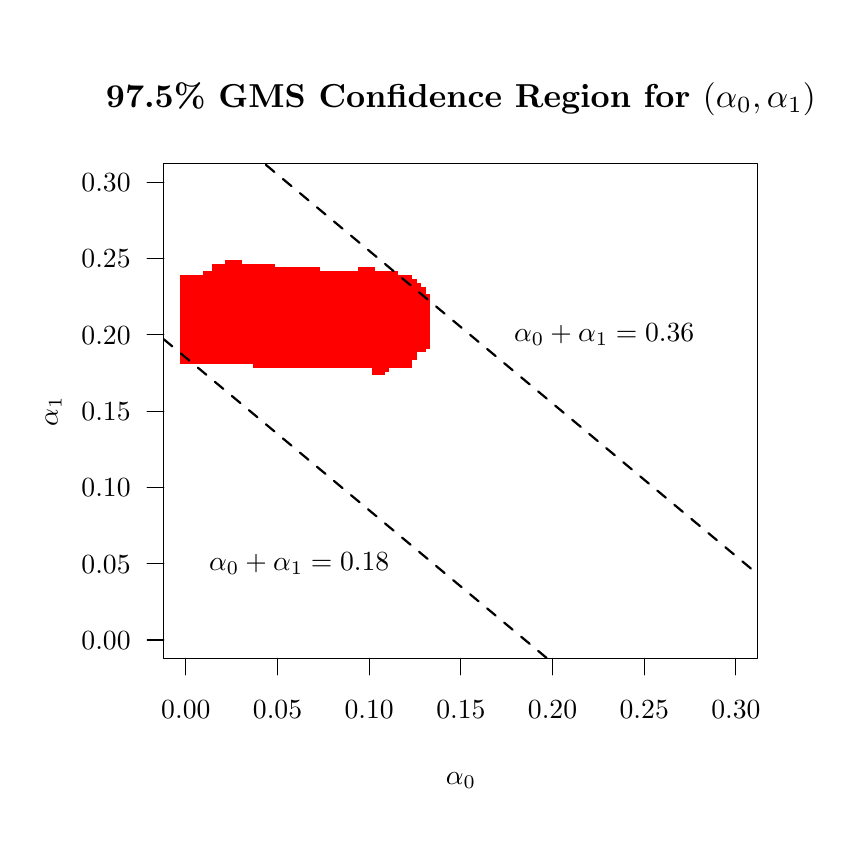
\begin{tikzpicture}[x=1pt,y=1pt]
\definecolor{fillColor}{RGB}{255,255,255}
\path[use as bounding box,fill=fillColor,fill opacity=0.00] (0,0) rectangle (289.08,289.08);
\begin{scope}
\path[clip] ( 49.20, 61.20) rectangle (263.88,239.88);
\definecolor{fillColor}{RGB}{255,0,0}

\path[fill=fillColor] (124.47,163.46) --
	(128.97,163.46) --
	(128.97,167.96) --
	(124.47,167.96) --
	cycle;

\path[fill=fillColor] (124.47,164.83) --
	(128.97,164.83) --
	(128.97,169.33) --
	(124.47,169.33) --
	cycle;

\path[fill=fillColor] (126.13,164.83) --
	(130.63,164.83) --
	(130.63,169.33) --
	(126.13,169.33) --
	cycle;

\path[fill=fillColor] ( 81.40,166.21) --
	( 85.90,166.21) --
	( 85.90,170.71) --
	( 81.40,170.71) --
	cycle;

\path[fill=fillColor] ( 83.06,166.21) --
	( 87.56,166.21) --
	( 87.56,170.71) --
	( 83.06,170.71) --
	cycle;

\path[fill=fillColor] ( 84.72,166.21) --
	( 89.22,166.21) --
	( 89.22,170.71) --
	( 84.72,170.71) --
	cycle;

\path[fill=fillColor] ( 86.37,166.21) --
	( 90.87,166.21) --
	( 90.87,170.71) --
	( 86.37,170.71) --
	cycle;

\path[fill=fillColor] ( 88.03,166.21) --
	( 92.53,166.21) --
	( 92.53,170.71) --
	( 88.03,170.71) --
	cycle;

\path[fill=fillColor] ( 89.69,166.21) --
	( 94.19,166.21) --
	( 94.19,170.71) --
	( 89.69,170.71) --
	cycle;

\path[fill=fillColor] ( 91.34,166.21) --
	( 95.84,166.21) --
	( 95.84,170.71) --
	( 91.34,170.71) --
	cycle;

\path[fill=fillColor] ( 93.00,166.21) --
	( 97.50,166.21) --
	( 97.50,170.71) --
	( 93.00,170.71) --
	cycle;

\path[fill=fillColor] ( 94.66,166.21) --
	( 99.16,166.21) --
	( 99.16,170.71) --
	( 94.66,170.71) --
	cycle;

\path[fill=fillColor] ( 96.31,166.21) --
	(100.81,166.21) --
	(100.81,170.71) --
	( 96.31,170.71) --
	cycle;

\path[fill=fillColor] ( 97.97,166.21) --
	(102.47,166.21) --
	(102.47,170.71) --
	( 97.97,170.71) --
	cycle;

\path[fill=fillColor] ( 99.63,166.21) --
	(104.13,166.21) --
	(104.13,170.71) --
	( 99.63,170.71) --
	cycle;

\path[fill=fillColor] (101.28,166.21) --
	(105.78,166.21) --
	(105.78,170.71) --
	(101.28,170.71) --
	cycle;

\path[fill=fillColor] (102.94,166.21) --
	(107.44,166.21) --
	(107.44,170.71) --
	(102.94,170.71) --
	cycle;

\path[fill=fillColor] (104.60,166.21) --
	(109.10,166.21) --
	(109.10,170.71) --
	(104.60,170.71) --
	cycle;

\path[fill=fillColor] (106.25,166.21) --
	(110.75,166.21) --
	(110.75,170.71) --
	(106.25,170.71) --
	cycle;

\path[fill=fillColor] (107.91,166.21) --
	(112.41,166.21) --
	(112.41,170.71) --
	(107.91,170.71) --
	cycle;

\path[fill=fillColor] (109.56,166.21) --
	(114.06,166.21) --
	(114.06,170.71) --
	(109.56,170.71) --
	cycle;

\path[fill=fillColor] (111.22,166.21) --
	(115.72,166.21) --
	(115.72,170.71) --
	(111.22,170.71) --
	cycle;

\path[fill=fillColor] (114.53,166.21) --
	(119.03,166.21) --
	(119.03,170.71) --
	(114.53,170.71) --
	cycle;

\path[fill=fillColor] (116.19,166.21) --
	(120.69,166.21) --
	(120.69,170.71) --
	(116.19,170.71) --
	cycle;

\path[fill=fillColor] (117.85,166.21) --
	(122.35,166.21) --
	(122.35,170.71) --
	(117.85,170.71) --
	cycle;

\path[fill=fillColor] (119.50,166.21) --
	(124.00,166.21) --
	(124.00,170.71) --
	(119.50,170.71) --
	cycle;

\path[fill=fillColor] (121.16,166.21) --
	(125.66,166.21) --
	(125.66,170.71) --
	(121.16,170.71) --
	cycle;

\path[fill=fillColor] (122.82,166.21) --
	(127.32,166.21) --
	(127.32,170.71) --
	(122.82,170.71) --
	cycle;

\path[fill=fillColor] (124.47,166.21) --
	(128.97,166.21) --
	(128.97,170.71) --
	(124.47,170.71) --
	cycle;

\path[fill=fillColor] (126.13,166.21) --
	(130.63,166.21) --
	(130.63,170.71) --
	(126.13,170.71) --
	cycle;

\path[fill=fillColor] (127.79,166.21) --
	(132.29,166.21) --
	(132.29,170.71) --
	(127.79,170.71) --
	cycle;

\path[fill=fillColor] (129.44,166.21) --
	(133.94,166.21) --
	(133.94,170.71) --
	(129.44,170.71) --
	cycle;

\path[fill=fillColor] (131.10,166.21) --
	(135.60,166.21) --
	(135.60,170.71) --
	(131.10,170.71) --
	cycle;

\path[fill=fillColor] (132.76,166.21) --
	(137.26,166.21) --
	(137.26,170.71) --
	(132.76,170.71) --
	cycle;

\path[fill=fillColor] (134.41,166.21) --
	(138.91,166.21) --
	(138.91,170.71) --
	(134.41,170.71) --
	cycle;

\path[fill=fillColor] ( 54.90,167.59) --
	( 59.40,167.59) --
	( 59.40,172.09) --
	( 54.90,172.09) --
	cycle;

\path[fill=fillColor] ( 56.56,167.59) --
	( 61.06,167.59) --
	( 61.06,172.09) --
	( 56.56,172.09) --
	cycle;

\path[fill=fillColor] ( 58.21,167.59) --
	( 62.71,167.59) --
	( 62.71,172.09) --
	( 58.21,172.09) --
	cycle;

\path[fill=fillColor] ( 59.87,167.59) --
	( 64.37,167.59) --
	( 64.37,172.09) --
	( 59.87,172.09) --
	cycle;

\path[fill=fillColor] ( 61.53,167.59) --
	( 66.03,167.59) --
	( 66.03,172.09) --
	( 61.53,172.09) --
	cycle;

\path[fill=fillColor] ( 63.18,167.59) --
	( 67.68,167.59) --
	( 67.68,172.09) --
	( 63.18,172.09) --
	cycle;

\path[fill=fillColor] ( 64.84,167.59) --
	( 69.34,167.59) --
	( 69.34,172.09) --
	( 64.84,172.09) --
	cycle;

\path[fill=fillColor] ( 66.50,167.59) --
	( 71.00,167.59) --
	( 71.00,172.09) --
	( 66.50,172.09) --
	cycle;

\path[fill=fillColor] ( 68.15,167.59) --
	( 72.65,167.59) --
	( 72.65,172.09) --
	( 68.15,172.09) --
	cycle;

\path[fill=fillColor] ( 69.81,167.59) --
	( 74.31,167.59) --
	( 74.31,172.09) --
	( 69.81,172.09) --
	cycle;

\path[fill=fillColor] ( 71.47,167.59) --
	( 75.97,167.59) --
	( 75.97,172.09) --
	( 71.47,172.09) --
	cycle;

\path[fill=fillColor] ( 73.12,167.59) --
	( 77.62,167.59) --
	( 77.62,172.09) --
	( 73.12,172.09) --
	cycle;

\path[fill=fillColor] ( 74.78,167.59) --
	( 79.28,167.59) --
	( 79.28,172.09) --
	( 74.78,172.09) --
	cycle;

\path[fill=fillColor] ( 76.44,167.59) --
	( 80.94,167.59) --
	( 80.94,172.09) --
	( 76.44,172.09) --
	cycle;

\path[fill=fillColor] ( 78.09,167.59) --
	( 82.59,167.59) --
	( 82.59,172.09) --
	( 78.09,172.09) --
	cycle;

\path[fill=fillColor] ( 79.75,167.59) --
	( 84.25,167.59) --
	( 84.25,172.09) --
	( 79.75,172.09) --
	cycle;

\path[fill=fillColor] ( 81.40,167.59) --
	( 85.90,167.59) --
	( 85.90,172.09) --
	( 81.40,172.09) --
	cycle;

\path[fill=fillColor] ( 83.06,167.59) --
	( 87.56,167.59) --
	( 87.56,172.09) --
	( 83.06,172.09) --
	cycle;

\path[fill=fillColor] ( 84.72,167.59) --
	( 89.22,167.59) --
	( 89.22,172.09) --
	( 84.72,172.09) --
	cycle;

\path[fill=fillColor] ( 86.37,167.59) --
	( 90.87,167.59) --
	( 90.87,172.09) --
	( 86.37,172.09) --
	cycle;

\path[fill=fillColor] ( 88.03,167.59) --
	( 92.53,167.59) --
	( 92.53,172.09) --
	( 88.03,172.09) --
	cycle;

\path[fill=fillColor] ( 89.69,167.59) --
	( 94.19,167.59) --
	( 94.19,172.09) --
	( 89.69,172.09) --
	cycle;

\path[fill=fillColor] ( 91.34,167.59) --
	( 95.84,167.59) --
	( 95.84,172.09) --
	( 91.34,172.09) --
	cycle;

\path[fill=fillColor] ( 93.00,167.59) --
	( 97.50,167.59) --
	( 97.50,172.09) --
	( 93.00,172.09) --
	cycle;

\path[fill=fillColor] ( 94.66,167.59) --
	( 99.16,167.59) --
	( 99.16,172.09) --
	( 94.66,172.09) --
	cycle;

\path[fill=fillColor] ( 96.31,167.59) --
	(100.81,167.59) --
	(100.81,172.09) --
	( 96.31,172.09) --
	cycle;

\path[fill=fillColor] ( 97.97,167.59) --
	(102.47,167.59) --
	(102.47,172.09) --
	( 97.97,172.09) --
	cycle;

\path[fill=fillColor] ( 99.63,167.59) --
	(104.13,167.59) --
	(104.13,172.09) --
	( 99.63,172.09) --
	cycle;

\path[fill=fillColor] (101.28,167.59) --
	(105.78,167.59) --
	(105.78,172.09) --
	(101.28,172.09) --
	cycle;

\path[fill=fillColor] (102.94,167.59) --
	(107.44,167.59) --
	(107.44,172.09) --
	(102.94,172.09) --
	cycle;

\path[fill=fillColor] (104.60,167.59) --
	(109.10,167.59) --
	(109.10,172.09) --
	(104.60,172.09) --
	cycle;

\path[fill=fillColor] (106.25,167.59) --
	(110.75,167.59) --
	(110.75,172.09) --
	(106.25,172.09) --
	cycle;

\path[fill=fillColor] (107.91,167.59) --
	(112.41,167.59) --
	(112.41,172.09) --
	(107.91,172.09) --
	cycle;

\path[fill=fillColor] (109.56,167.59) --
	(114.06,167.59) --
	(114.06,172.09) --
	(109.56,172.09) --
	cycle;

\path[fill=fillColor] (111.22,167.59) --
	(115.72,167.59) --
	(115.72,172.09) --
	(111.22,172.09) --
	cycle;

\path[fill=fillColor] (112.88,167.59) --
	(117.38,167.59) --
	(117.38,172.09) --
	(112.88,172.09) --
	cycle;

\path[fill=fillColor] (114.53,167.59) --
	(119.03,167.59) --
	(119.03,172.09) --
	(114.53,172.09) --
	cycle;

\path[fill=fillColor] (116.19,167.59) --
	(120.69,167.59) --
	(120.69,172.09) --
	(116.19,172.09) --
	cycle;

\path[fill=fillColor] (117.85,167.59) --
	(122.35,167.59) --
	(122.35,172.09) --
	(117.85,172.09) --
	cycle;

\path[fill=fillColor] (119.50,167.59) --
	(124.00,167.59) --
	(124.00,172.09) --
	(119.50,172.09) --
	cycle;

\path[fill=fillColor] (121.16,167.59) --
	(125.66,167.59) --
	(125.66,172.09) --
	(121.16,172.09) --
	cycle;

\path[fill=fillColor] (122.82,167.59) --
	(127.32,167.59) --
	(127.32,172.09) --
	(122.82,172.09) --
	cycle;

\path[fill=fillColor] (124.47,167.59) --
	(128.97,167.59) --
	(128.97,172.09) --
	(124.47,172.09) --
	cycle;

\path[fill=fillColor] (126.13,167.59) --
	(130.63,167.59) --
	(130.63,172.09) --
	(126.13,172.09) --
	cycle;

\path[fill=fillColor] (127.79,167.59) --
	(132.29,167.59) --
	(132.29,172.09) --
	(127.79,172.09) --
	cycle;

\path[fill=fillColor] (129.44,167.59) --
	(133.94,167.59) --
	(133.94,172.09) --
	(129.44,172.09) --
	cycle;

\path[fill=fillColor] (131.10,167.59) --
	(135.60,167.59) --
	(135.60,172.09) --
	(131.10,172.09) --
	cycle;

\path[fill=fillColor] (132.76,167.59) --
	(137.26,167.59) --
	(137.26,172.09) --
	(132.76,172.09) --
	cycle;

\path[fill=fillColor] (134.41,167.59) --
	(138.91,167.59) --
	(138.91,172.09) --
	(134.41,172.09) --
	cycle;

\path[fill=fillColor] ( 54.90,168.97) --
	( 59.40,168.97) --
	( 59.40,173.47) --
	( 54.90,173.47) --
	cycle;

\path[fill=fillColor] ( 56.56,168.97) --
	( 61.06,168.97) --
	( 61.06,173.47) --
	( 56.56,173.47) --
	cycle;

\path[fill=fillColor] ( 58.21,168.97) --
	( 62.71,168.97) --
	( 62.71,173.47) --
	( 58.21,173.47) --
	cycle;

\path[fill=fillColor] ( 59.87,168.97) --
	( 64.37,168.97) --
	( 64.37,173.47) --
	( 59.87,173.47) --
	cycle;

\path[fill=fillColor] ( 61.53,168.97) --
	( 66.03,168.97) --
	( 66.03,173.47) --
	( 61.53,173.47) --
	cycle;

\path[fill=fillColor] ( 63.18,168.97) --
	( 67.68,168.97) --
	( 67.68,173.47) --
	( 63.18,173.47) --
	cycle;

\path[fill=fillColor] ( 64.84,168.97) --
	( 69.34,168.97) --
	( 69.34,173.47) --
	( 64.84,173.47) --
	cycle;

\path[fill=fillColor] ( 66.50,168.97) --
	( 71.00,168.97) --
	( 71.00,173.47) --
	( 66.50,173.47) --
	cycle;

\path[fill=fillColor] ( 68.15,168.97) --
	( 72.65,168.97) --
	( 72.65,173.47) --
	( 68.15,173.47) --
	cycle;

\path[fill=fillColor] ( 69.81,168.97) --
	( 74.31,168.97) --
	( 74.31,173.47) --
	( 69.81,173.47) --
	cycle;

\path[fill=fillColor] ( 71.47,168.97) --
	( 75.97,168.97) --
	( 75.97,173.47) --
	( 71.47,173.47) --
	cycle;

\path[fill=fillColor] ( 73.12,168.97) --
	( 77.62,168.97) --
	( 77.62,173.47) --
	( 73.12,173.47) --
	cycle;

\path[fill=fillColor] ( 74.78,168.97) --
	( 79.28,168.97) --
	( 79.28,173.47) --
	( 74.78,173.47) --
	cycle;

\path[fill=fillColor] ( 76.44,168.97) --
	( 80.94,168.97) --
	( 80.94,173.47) --
	( 76.44,173.47) --
	cycle;

\path[fill=fillColor] ( 78.09,168.97) --
	( 82.59,168.97) --
	( 82.59,173.47) --
	( 78.09,173.47) --
	cycle;

\path[fill=fillColor] ( 79.75,168.97) --
	( 84.25,168.97) --
	( 84.25,173.47) --
	( 79.75,173.47) --
	cycle;

\path[fill=fillColor] ( 81.40,168.97) --
	( 85.90,168.97) --
	( 85.90,173.47) --
	( 81.40,173.47) --
	cycle;

\path[fill=fillColor] ( 83.06,168.97) --
	( 87.56,168.97) --
	( 87.56,173.47) --
	( 83.06,173.47) --
	cycle;

\path[fill=fillColor] ( 84.72,168.97) --
	( 89.22,168.97) --
	( 89.22,173.47) --
	( 84.72,173.47) --
	cycle;

\path[fill=fillColor] ( 86.37,168.97) --
	( 90.87,168.97) --
	( 90.87,173.47) --
	( 86.37,173.47) --
	cycle;

\path[fill=fillColor] ( 88.03,168.97) --
	( 92.53,168.97) --
	( 92.53,173.47) --
	( 88.03,173.47) --
	cycle;

\path[fill=fillColor] ( 89.69,168.97) --
	( 94.19,168.97) --
	( 94.19,173.47) --
	( 89.69,173.47) --
	cycle;

\path[fill=fillColor] ( 91.34,168.97) --
	( 95.84,168.97) --
	( 95.84,173.47) --
	( 91.34,173.47) --
	cycle;

\path[fill=fillColor] ( 93.00,168.97) --
	( 97.50,168.97) --
	( 97.50,173.47) --
	( 93.00,173.47) --
	cycle;

\path[fill=fillColor] ( 94.66,168.97) --
	( 99.16,168.97) --
	( 99.16,173.47) --
	( 94.66,173.47) --
	cycle;

\path[fill=fillColor] ( 96.31,168.97) --
	(100.81,168.97) --
	(100.81,173.47) --
	( 96.31,173.47) --
	cycle;

\path[fill=fillColor] ( 97.97,168.97) --
	(102.47,168.97) --
	(102.47,173.47) --
	( 97.97,173.47) --
	cycle;

\path[fill=fillColor] ( 99.63,168.97) --
	(104.13,168.97) --
	(104.13,173.47) --
	( 99.63,173.47) --
	cycle;

\path[fill=fillColor] (101.28,168.97) --
	(105.78,168.97) --
	(105.78,173.47) --
	(101.28,173.47) --
	cycle;

\path[fill=fillColor] (102.94,168.97) --
	(107.44,168.97) --
	(107.44,173.47) --
	(102.94,173.47) --
	cycle;

\path[fill=fillColor] (104.60,168.97) --
	(109.10,168.97) --
	(109.10,173.47) --
	(104.60,173.47) --
	cycle;

\path[fill=fillColor] (106.25,168.97) --
	(110.75,168.97) --
	(110.75,173.47) --
	(106.25,173.47) --
	cycle;

\path[fill=fillColor] (107.91,168.97) --
	(112.41,168.97) --
	(112.41,173.47) --
	(107.91,173.47) --
	cycle;

\path[fill=fillColor] (109.56,168.97) --
	(114.06,168.97) --
	(114.06,173.47) --
	(109.56,173.47) --
	cycle;

\path[fill=fillColor] (111.22,168.97) --
	(115.72,168.97) --
	(115.72,173.47) --
	(111.22,173.47) --
	cycle;

\path[fill=fillColor] (112.88,168.97) --
	(117.38,168.97) --
	(117.38,173.47) --
	(112.88,173.47) --
	cycle;

\path[fill=fillColor] (114.53,168.97) --
	(119.03,168.97) --
	(119.03,173.47) --
	(114.53,173.47) --
	cycle;

\path[fill=fillColor] (116.19,168.97) --
	(120.69,168.97) --
	(120.69,173.47) --
	(116.19,173.47) --
	cycle;

\path[fill=fillColor] (117.85,168.97) --
	(122.35,168.97) --
	(122.35,173.47) --
	(117.85,173.47) --
	cycle;

\path[fill=fillColor] (119.50,168.97) --
	(124.00,168.97) --
	(124.00,173.47) --
	(119.50,173.47) --
	cycle;

\path[fill=fillColor] (121.16,168.97) --
	(125.66,168.97) --
	(125.66,173.47) --
	(121.16,173.47) --
	cycle;

\path[fill=fillColor] (122.82,168.97) --
	(127.32,168.97) --
	(127.32,173.47) --
	(122.82,173.47) --
	cycle;

\path[fill=fillColor] (124.47,168.97) --
	(128.97,168.97) --
	(128.97,173.47) --
	(124.47,173.47) --
	cycle;

\path[fill=fillColor] (126.13,168.97) --
	(130.63,168.97) --
	(130.63,173.47) --
	(126.13,173.47) --
	cycle;

\path[fill=fillColor] (127.79,168.97) --
	(132.29,168.97) --
	(132.29,173.47) --
	(127.79,173.47) --
	cycle;

\path[fill=fillColor] (129.44,168.97) --
	(133.94,168.97) --
	(133.94,173.47) --
	(129.44,173.47) --
	cycle;

\path[fill=fillColor] (131.10,168.97) --
	(135.60,168.97) --
	(135.60,173.47) --
	(131.10,173.47) --
	cycle;

\path[fill=fillColor] (132.76,168.97) --
	(137.26,168.97) --
	(137.26,173.47) --
	(132.76,173.47) --
	cycle;

\path[fill=fillColor] (134.41,168.97) --
	(138.91,168.97) --
	(138.91,173.47) --
	(134.41,173.47) --
	cycle;

\path[fill=fillColor] (136.07,168.97) --
	(140.57,168.97) --
	(140.57,173.47) --
	(136.07,173.47) --
	cycle;

\path[fill=fillColor] ( 54.90,170.35) --
	( 59.40,170.35) --
	( 59.40,174.85) --
	( 54.90,174.85) --
	cycle;

\path[fill=fillColor] ( 56.56,170.35) --
	( 61.06,170.35) --
	( 61.06,174.85) --
	( 56.56,174.85) --
	cycle;

\path[fill=fillColor] ( 58.21,170.35) --
	( 62.71,170.35) --
	( 62.71,174.85) --
	( 58.21,174.85) --
	cycle;

\path[fill=fillColor] ( 59.87,170.35) --
	( 64.37,170.35) --
	( 64.37,174.85) --
	( 59.87,174.85) --
	cycle;

\path[fill=fillColor] ( 61.53,170.35) --
	( 66.03,170.35) --
	( 66.03,174.85) --
	( 61.53,174.85) --
	cycle;

\path[fill=fillColor] ( 63.18,170.35) --
	( 67.68,170.35) --
	( 67.68,174.85) --
	( 63.18,174.85) --
	cycle;

\path[fill=fillColor] ( 64.84,170.35) --
	( 69.34,170.35) --
	( 69.34,174.85) --
	( 64.84,174.85) --
	cycle;

\path[fill=fillColor] ( 66.50,170.35) --
	( 71.00,170.35) --
	( 71.00,174.85) --
	( 66.50,174.85) --
	cycle;

\path[fill=fillColor] ( 68.15,170.35) --
	( 72.65,170.35) --
	( 72.65,174.85) --
	( 68.15,174.85) --
	cycle;

\path[fill=fillColor] ( 69.81,170.35) --
	( 74.31,170.35) --
	( 74.31,174.85) --
	( 69.81,174.85) --
	cycle;

\path[fill=fillColor] ( 71.47,170.35) --
	( 75.97,170.35) --
	( 75.97,174.85) --
	( 71.47,174.85) --
	cycle;

\path[fill=fillColor] ( 73.12,170.35) --
	( 77.62,170.35) --
	( 77.62,174.85) --
	( 73.12,174.85) --
	cycle;

\path[fill=fillColor] ( 74.78,170.35) --
	( 79.28,170.35) --
	( 79.28,174.85) --
	( 74.78,174.85) --
	cycle;

\path[fill=fillColor] ( 76.44,170.35) --
	( 80.94,170.35) --
	( 80.94,174.85) --
	( 76.44,174.85) --
	cycle;

\path[fill=fillColor] ( 78.09,170.35) --
	( 82.59,170.35) --
	( 82.59,174.85) --
	( 78.09,174.85) --
	cycle;

\path[fill=fillColor] ( 79.75,170.35) --
	( 84.25,170.35) --
	( 84.25,174.85) --
	( 79.75,174.85) --
	cycle;

\path[fill=fillColor] ( 81.40,170.35) --
	( 85.90,170.35) --
	( 85.90,174.85) --
	( 81.40,174.85) --
	cycle;

\path[fill=fillColor] ( 83.06,170.35) --
	( 87.56,170.35) --
	( 87.56,174.85) --
	( 83.06,174.85) --
	cycle;

\path[fill=fillColor] ( 84.72,170.35) --
	( 89.22,170.35) --
	( 89.22,174.85) --
	( 84.72,174.85) --
	cycle;

\path[fill=fillColor] ( 86.37,170.35) --
	( 90.87,170.35) --
	( 90.87,174.85) --
	( 86.37,174.85) --
	cycle;

\path[fill=fillColor] ( 88.03,170.35) --
	( 92.53,170.35) --
	( 92.53,174.85) --
	( 88.03,174.85) --
	cycle;

\path[fill=fillColor] ( 89.69,170.35) --
	( 94.19,170.35) --
	( 94.19,174.85) --
	( 89.69,174.85) --
	cycle;

\path[fill=fillColor] ( 91.34,170.35) --
	( 95.84,170.35) --
	( 95.84,174.85) --
	( 91.34,174.85) --
	cycle;

\path[fill=fillColor] ( 93.00,170.35) --
	( 97.50,170.35) --
	( 97.50,174.85) --
	( 93.00,174.85) --
	cycle;

\path[fill=fillColor] ( 94.66,170.35) --
	( 99.16,170.35) --
	( 99.16,174.85) --
	( 94.66,174.85) --
	cycle;

\path[fill=fillColor] ( 96.31,170.35) --
	(100.81,170.35) --
	(100.81,174.85) --
	( 96.31,174.85) --
	cycle;

\path[fill=fillColor] ( 97.97,170.35) --
	(102.47,170.35) --
	(102.47,174.85) --
	( 97.97,174.85) --
	cycle;

\path[fill=fillColor] ( 99.63,170.35) --
	(104.13,170.35) --
	(104.13,174.85) --
	( 99.63,174.85) --
	cycle;

\path[fill=fillColor] (101.28,170.35) --
	(105.78,170.35) --
	(105.78,174.85) --
	(101.28,174.85) --
	cycle;

\path[fill=fillColor] (102.94,170.35) --
	(107.44,170.35) --
	(107.44,174.85) --
	(102.94,174.85) --
	cycle;

\path[fill=fillColor] (104.60,170.35) --
	(109.10,170.35) --
	(109.10,174.85) --
	(104.60,174.85) --
	cycle;

\path[fill=fillColor] (106.25,170.35) --
	(110.75,170.35) --
	(110.75,174.85) --
	(106.25,174.85) --
	cycle;

\path[fill=fillColor] (107.91,170.35) --
	(112.41,170.35) --
	(112.41,174.85) --
	(107.91,174.85) --
	cycle;

\path[fill=fillColor] (109.56,170.35) --
	(114.06,170.35) --
	(114.06,174.85) --
	(109.56,174.85) --
	cycle;

\path[fill=fillColor] (111.22,170.35) --
	(115.72,170.35) --
	(115.72,174.85) --
	(111.22,174.85) --
	cycle;

\path[fill=fillColor] (112.88,170.35) --
	(117.38,170.35) --
	(117.38,174.85) --
	(112.88,174.85) --
	cycle;

\path[fill=fillColor] (114.53,170.35) --
	(119.03,170.35) --
	(119.03,174.85) --
	(114.53,174.85) --
	cycle;

\path[fill=fillColor] (116.19,170.35) --
	(120.69,170.35) --
	(120.69,174.85) --
	(116.19,174.85) --
	cycle;

\path[fill=fillColor] (117.85,170.35) --
	(122.35,170.35) --
	(122.35,174.85) --
	(117.85,174.85) --
	cycle;

\path[fill=fillColor] (119.50,170.35) --
	(124.00,170.35) --
	(124.00,174.85) --
	(119.50,174.85) --
	cycle;

\path[fill=fillColor] (121.16,170.35) --
	(125.66,170.35) --
	(125.66,174.85) --
	(121.16,174.85) --
	cycle;

\path[fill=fillColor] (122.82,170.35) --
	(127.32,170.35) --
	(127.32,174.85) --
	(122.82,174.85) --
	cycle;

\path[fill=fillColor] (124.47,170.35) --
	(128.97,170.35) --
	(128.97,174.85) --
	(124.47,174.85) --
	cycle;

\path[fill=fillColor] (126.13,170.35) --
	(130.63,170.35) --
	(130.63,174.85) --
	(126.13,174.85) --
	cycle;

\path[fill=fillColor] (127.79,170.35) --
	(132.29,170.35) --
	(132.29,174.85) --
	(127.79,174.85) --
	cycle;

\path[fill=fillColor] (129.44,170.35) --
	(133.94,170.35) --
	(133.94,174.85) --
	(129.44,174.85) --
	cycle;

\path[fill=fillColor] (131.10,170.35) --
	(135.60,170.35) --
	(135.60,174.85) --
	(131.10,174.85) --
	cycle;

\path[fill=fillColor] (132.76,170.35) --
	(137.26,170.35) --
	(137.26,174.85) --
	(132.76,174.85) --
	cycle;

\path[fill=fillColor] (134.41,170.35) --
	(138.91,170.35) --
	(138.91,174.85) --
	(134.41,174.85) --
	cycle;

\path[fill=fillColor] (136.07,170.35) --
	(140.57,170.35) --
	(140.57,174.85) --
	(136.07,174.85) --
	cycle;

\path[fill=fillColor] ( 54.90,171.73) --
	( 59.40,171.73) --
	( 59.40,176.23) --
	( 54.90,176.23) --
	cycle;

\path[fill=fillColor] ( 56.56,171.73) --
	( 61.06,171.73) --
	( 61.06,176.23) --
	( 56.56,176.23) --
	cycle;

\path[fill=fillColor] ( 58.21,171.73) --
	( 62.71,171.73) --
	( 62.71,176.23) --
	( 58.21,176.23) --
	cycle;

\path[fill=fillColor] ( 59.87,171.73) --
	( 64.37,171.73) --
	( 64.37,176.23) --
	( 59.87,176.23) --
	cycle;

\path[fill=fillColor] ( 61.53,171.73) --
	( 66.03,171.73) --
	( 66.03,176.23) --
	( 61.53,176.23) --
	cycle;

\path[fill=fillColor] ( 63.18,171.73) --
	( 67.68,171.73) --
	( 67.68,176.23) --
	( 63.18,176.23) --
	cycle;

\path[fill=fillColor] ( 64.84,171.73) --
	( 69.34,171.73) --
	( 69.34,176.23) --
	( 64.84,176.23) --
	cycle;

\path[fill=fillColor] ( 66.50,171.73) --
	( 71.00,171.73) --
	( 71.00,176.23) --
	( 66.50,176.23) --
	cycle;

\path[fill=fillColor] ( 68.15,171.73) --
	( 72.65,171.73) --
	( 72.65,176.23) --
	( 68.15,176.23) --
	cycle;

\path[fill=fillColor] ( 69.81,171.73) --
	( 74.31,171.73) --
	( 74.31,176.23) --
	( 69.81,176.23) --
	cycle;

\path[fill=fillColor] ( 71.47,171.73) --
	( 75.97,171.73) --
	( 75.97,176.23) --
	( 71.47,176.23) --
	cycle;

\path[fill=fillColor] ( 73.12,171.73) --
	( 77.62,171.73) --
	( 77.62,176.23) --
	( 73.12,176.23) --
	cycle;

\path[fill=fillColor] ( 74.78,171.73) --
	( 79.28,171.73) --
	( 79.28,176.23) --
	( 74.78,176.23) --
	cycle;

\path[fill=fillColor] ( 76.44,171.73) --
	( 80.94,171.73) --
	( 80.94,176.23) --
	( 76.44,176.23) --
	cycle;

\path[fill=fillColor] ( 78.09,171.73) --
	( 82.59,171.73) --
	( 82.59,176.23) --
	( 78.09,176.23) --
	cycle;

\path[fill=fillColor] ( 79.75,171.73) --
	( 84.25,171.73) --
	( 84.25,176.23) --
	( 79.75,176.23) --
	cycle;

\path[fill=fillColor] ( 81.40,171.73) --
	( 85.90,171.73) --
	( 85.90,176.23) --
	( 81.40,176.23) --
	cycle;

\path[fill=fillColor] ( 83.06,171.73) --
	( 87.56,171.73) --
	( 87.56,176.23) --
	( 83.06,176.23) --
	cycle;

\path[fill=fillColor] ( 84.72,171.73) --
	( 89.22,171.73) --
	( 89.22,176.23) --
	( 84.72,176.23) --
	cycle;

\path[fill=fillColor] ( 86.37,171.73) --
	( 90.87,171.73) --
	( 90.87,176.23) --
	( 86.37,176.23) --
	cycle;

\path[fill=fillColor] ( 88.03,171.73) --
	( 92.53,171.73) --
	( 92.53,176.23) --
	( 88.03,176.23) --
	cycle;

\path[fill=fillColor] ( 89.69,171.73) --
	( 94.19,171.73) --
	( 94.19,176.23) --
	( 89.69,176.23) --
	cycle;

\path[fill=fillColor] ( 91.34,171.73) --
	( 95.84,171.73) --
	( 95.84,176.23) --
	( 91.34,176.23) --
	cycle;

\path[fill=fillColor] ( 93.00,171.73) --
	( 97.50,171.73) --
	( 97.50,176.23) --
	( 93.00,176.23) --
	cycle;

\path[fill=fillColor] ( 94.66,171.73) --
	( 99.16,171.73) --
	( 99.16,176.23) --
	( 94.66,176.23) --
	cycle;

\path[fill=fillColor] ( 96.31,171.73) --
	(100.81,171.73) --
	(100.81,176.23) --
	( 96.31,176.23) --
	cycle;

\path[fill=fillColor] ( 97.97,171.73) --
	(102.47,171.73) --
	(102.47,176.23) --
	( 97.97,176.23) --
	cycle;

\path[fill=fillColor] ( 99.63,171.73) --
	(104.13,171.73) --
	(104.13,176.23) --
	( 99.63,176.23) --
	cycle;

\path[fill=fillColor] (101.28,171.73) --
	(105.78,171.73) --
	(105.78,176.23) --
	(101.28,176.23) --
	cycle;

\path[fill=fillColor] (102.94,171.73) --
	(107.44,171.73) --
	(107.44,176.23) --
	(102.94,176.23) --
	cycle;

\path[fill=fillColor] (104.60,171.73) --
	(109.10,171.73) --
	(109.10,176.23) --
	(104.60,176.23) --
	cycle;

\path[fill=fillColor] (106.25,171.73) --
	(110.75,171.73) --
	(110.75,176.23) --
	(106.25,176.23) --
	cycle;

\path[fill=fillColor] (107.91,171.73) --
	(112.41,171.73) --
	(112.41,176.23) --
	(107.91,176.23) --
	cycle;

\path[fill=fillColor] (109.56,171.73) --
	(114.06,171.73) --
	(114.06,176.23) --
	(109.56,176.23) --
	cycle;

\path[fill=fillColor] (111.22,171.73) --
	(115.72,171.73) --
	(115.72,176.23) --
	(111.22,176.23) --
	cycle;

\path[fill=fillColor] (112.88,171.73) --
	(117.38,171.73) --
	(117.38,176.23) --
	(112.88,176.23) --
	cycle;

\path[fill=fillColor] (114.53,171.73) --
	(119.03,171.73) --
	(119.03,176.23) --
	(114.53,176.23) --
	cycle;

\path[fill=fillColor] (116.19,171.73) --
	(120.69,171.73) --
	(120.69,176.23) --
	(116.19,176.23) --
	cycle;

\path[fill=fillColor] (117.85,171.73) --
	(122.35,171.73) --
	(122.35,176.23) --
	(117.85,176.23) --
	cycle;

\path[fill=fillColor] (119.50,171.73) --
	(124.00,171.73) --
	(124.00,176.23) --
	(119.50,176.23) --
	cycle;

\path[fill=fillColor] (121.16,171.73) --
	(125.66,171.73) --
	(125.66,176.23) --
	(121.16,176.23) --
	cycle;

\path[fill=fillColor] (122.82,171.73) --
	(127.32,171.73) --
	(127.32,176.23) --
	(122.82,176.23) --
	cycle;

\path[fill=fillColor] (124.47,171.73) --
	(128.97,171.73) --
	(128.97,176.23) --
	(124.47,176.23) --
	cycle;

\path[fill=fillColor] (126.13,171.73) --
	(130.63,171.73) --
	(130.63,176.23) --
	(126.13,176.23) --
	cycle;

\path[fill=fillColor] (127.79,171.73) --
	(132.29,171.73) --
	(132.29,176.23) --
	(127.79,176.23) --
	cycle;

\path[fill=fillColor] (129.44,171.73) --
	(133.94,171.73) --
	(133.94,176.23) --
	(129.44,176.23) --
	cycle;

\path[fill=fillColor] (131.10,171.73) --
	(135.60,171.73) --
	(135.60,176.23) --
	(131.10,176.23) --
	cycle;

\path[fill=fillColor] (132.76,171.73) --
	(137.26,171.73) --
	(137.26,176.23) --
	(132.76,176.23) --
	cycle;

\path[fill=fillColor] (134.41,171.73) --
	(138.91,171.73) --
	(138.91,176.23) --
	(134.41,176.23) --
	cycle;

\path[fill=fillColor] (136.07,171.73) --
	(140.57,171.73) --
	(140.57,176.23) --
	(136.07,176.23) --
	cycle;

\path[fill=fillColor] (137.73,171.73) --
	(142.23,171.73) --
	(142.23,176.23) --
	(137.73,176.23) --
	cycle;

\path[fill=fillColor] (139.38,171.73) --
	(143.88,171.73) --
	(143.88,176.23) --
	(139.38,176.23) --
	cycle;

\path[fill=fillColor] ( 54.90,173.11) --
	( 59.40,173.11) --
	( 59.40,177.61) --
	( 54.90,177.61) --
	cycle;

\path[fill=fillColor] ( 56.56,173.11) --
	( 61.06,173.11) --
	( 61.06,177.61) --
	( 56.56,177.61) --
	cycle;

\path[fill=fillColor] ( 58.21,173.11) --
	( 62.71,173.11) --
	( 62.71,177.61) --
	( 58.21,177.61) --
	cycle;

\path[fill=fillColor] ( 59.87,173.11) --
	( 64.37,173.11) --
	( 64.37,177.61) --
	( 59.87,177.61) --
	cycle;

\path[fill=fillColor] ( 61.53,173.11) --
	( 66.03,173.11) --
	( 66.03,177.61) --
	( 61.53,177.61) --
	cycle;

\path[fill=fillColor] ( 63.18,173.11) --
	( 67.68,173.11) --
	( 67.68,177.61) --
	( 63.18,177.61) --
	cycle;

\path[fill=fillColor] ( 64.84,173.11) --
	( 69.34,173.11) --
	( 69.34,177.61) --
	( 64.84,177.61) --
	cycle;

\path[fill=fillColor] ( 66.50,173.11) --
	( 71.00,173.11) --
	( 71.00,177.61) --
	( 66.50,177.61) --
	cycle;

\path[fill=fillColor] ( 68.15,173.11) --
	( 72.65,173.11) --
	( 72.65,177.61) --
	( 68.15,177.61) --
	cycle;

\path[fill=fillColor] ( 69.81,173.11) --
	( 74.31,173.11) --
	( 74.31,177.61) --
	( 69.81,177.61) --
	cycle;

\path[fill=fillColor] ( 71.47,173.11) --
	( 75.97,173.11) --
	( 75.97,177.61) --
	( 71.47,177.61) --
	cycle;

\path[fill=fillColor] ( 73.12,173.11) --
	( 77.62,173.11) --
	( 77.62,177.61) --
	( 73.12,177.61) --
	cycle;

\path[fill=fillColor] ( 74.78,173.11) --
	( 79.28,173.11) --
	( 79.28,177.61) --
	( 74.78,177.61) --
	cycle;

\path[fill=fillColor] ( 76.44,173.11) --
	( 80.94,173.11) --
	( 80.94,177.61) --
	( 76.44,177.61) --
	cycle;

\path[fill=fillColor] ( 78.09,173.11) --
	( 82.59,173.11) --
	( 82.59,177.61) --
	( 78.09,177.61) --
	cycle;

\path[fill=fillColor] ( 79.75,173.11) --
	( 84.25,173.11) --
	( 84.25,177.61) --
	( 79.75,177.61) --
	cycle;

\path[fill=fillColor] ( 81.40,173.11) --
	( 85.90,173.11) --
	( 85.90,177.61) --
	( 81.40,177.61) --
	cycle;

\path[fill=fillColor] ( 83.06,173.11) --
	( 87.56,173.11) --
	( 87.56,177.61) --
	( 83.06,177.61) --
	cycle;

\path[fill=fillColor] ( 84.72,173.11) --
	( 89.22,173.11) --
	( 89.22,177.61) --
	( 84.72,177.61) --
	cycle;

\path[fill=fillColor] ( 86.37,173.11) --
	( 90.87,173.11) --
	( 90.87,177.61) --
	( 86.37,177.61) --
	cycle;

\path[fill=fillColor] ( 88.03,173.11) --
	( 92.53,173.11) --
	( 92.53,177.61) --
	( 88.03,177.61) --
	cycle;

\path[fill=fillColor] ( 89.69,173.11) --
	( 94.19,173.11) --
	( 94.19,177.61) --
	( 89.69,177.61) --
	cycle;

\path[fill=fillColor] ( 91.34,173.11) --
	( 95.84,173.11) --
	( 95.84,177.61) --
	( 91.34,177.61) --
	cycle;

\path[fill=fillColor] ( 93.00,173.11) --
	( 97.50,173.11) --
	( 97.50,177.61) --
	( 93.00,177.61) --
	cycle;

\path[fill=fillColor] ( 94.66,173.11) --
	( 99.16,173.11) --
	( 99.16,177.61) --
	( 94.66,177.61) --
	cycle;

\path[fill=fillColor] ( 96.31,173.11) --
	(100.81,173.11) --
	(100.81,177.61) --
	( 96.31,177.61) --
	cycle;

\path[fill=fillColor] ( 97.97,173.11) --
	(102.47,173.11) --
	(102.47,177.61) --
	( 97.97,177.61) --
	cycle;

\path[fill=fillColor] ( 99.63,173.11) --
	(104.13,173.11) --
	(104.13,177.61) --
	( 99.63,177.61) --
	cycle;

\path[fill=fillColor] (101.28,173.11) --
	(105.78,173.11) --
	(105.78,177.61) --
	(101.28,177.61) --
	cycle;

\path[fill=fillColor] (102.94,173.11) --
	(107.44,173.11) --
	(107.44,177.61) --
	(102.94,177.61) --
	cycle;

\path[fill=fillColor] (104.60,173.11) --
	(109.10,173.11) --
	(109.10,177.61) --
	(104.60,177.61) --
	cycle;

\path[fill=fillColor] (106.25,173.11) --
	(110.75,173.11) --
	(110.75,177.61) --
	(106.25,177.61) --
	cycle;

\path[fill=fillColor] (107.91,173.11) --
	(112.41,173.11) --
	(112.41,177.61) --
	(107.91,177.61) --
	cycle;

\path[fill=fillColor] (109.56,173.11) --
	(114.06,173.11) --
	(114.06,177.61) --
	(109.56,177.61) --
	cycle;

\path[fill=fillColor] (111.22,173.11) --
	(115.72,173.11) --
	(115.72,177.61) --
	(111.22,177.61) --
	cycle;

\path[fill=fillColor] (112.88,173.11) --
	(117.38,173.11) --
	(117.38,177.61) --
	(112.88,177.61) --
	cycle;

\path[fill=fillColor] (114.53,173.11) --
	(119.03,173.11) --
	(119.03,177.61) --
	(114.53,177.61) --
	cycle;

\path[fill=fillColor] (116.19,173.11) --
	(120.69,173.11) --
	(120.69,177.61) --
	(116.19,177.61) --
	cycle;

\path[fill=fillColor] (117.85,173.11) --
	(122.35,173.11) --
	(122.35,177.61) --
	(117.85,177.61) --
	cycle;

\path[fill=fillColor] (119.50,173.11) --
	(124.00,173.11) --
	(124.00,177.61) --
	(119.50,177.61) --
	cycle;

\path[fill=fillColor] (121.16,173.11) --
	(125.66,173.11) --
	(125.66,177.61) --
	(121.16,177.61) --
	cycle;

\path[fill=fillColor] (122.82,173.11) --
	(127.32,173.11) --
	(127.32,177.61) --
	(122.82,177.61) --
	cycle;

\path[fill=fillColor] (124.47,173.11) --
	(128.97,173.11) --
	(128.97,177.61) --
	(124.47,177.61) --
	cycle;

\path[fill=fillColor] (126.13,173.11) --
	(130.63,173.11) --
	(130.63,177.61) --
	(126.13,177.61) --
	cycle;

\path[fill=fillColor] (127.79,173.11) --
	(132.29,173.11) --
	(132.29,177.61) --
	(127.79,177.61) --
	cycle;

\path[fill=fillColor] (129.44,173.11) --
	(133.94,173.11) --
	(133.94,177.61) --
	(129.44,177.61) --
	cycle;

\path[fill=fillColor] (131.10,173.11) --
	(135.60,173.11) --
	(135.60,177.61) --
	(131.10,177.61) --
	cycle;

\path[fill=fillColor] (132.76,173.11) --
	(137.26,173.11) --
	(137.26,177.61) --
	(132.76,177.61) --
	cycle;

\path[fill=fillColor] (134.41,173.11) --
	(138.91,173.11) --
	(138.91,177.61) --
	(134.41,177.61) --
	cycle;

\path[fill=fillColor] (136.07,173.11) --
	(140.57,173.11) --
	(140.57,177.61) --
	(136.07,177.61) --
	cycle;

\path[fill=fillColor] (137.73,173.11) --
	(142.23,173.11) --
	(142.23,177.61) --
	(137.73,177.61) --
	cycle;

\path[fill=fillColor] (139.38,173.11) --
	(143.88,173.11) --
	(143.88,177.61) --
	(139.38,177.61) --
	cycle;

\path[fill=fillColor] (141.04,173.11) --
	(145.54,173.11) --
	(145.54,177.61) --
	(141.04,177.61) --
	cycle;

\path[fill=fillColor] ( 54.90,174.49) --
	( 59.40,174.49) --
	( 59.40,178.99) --
	( 54.90,178.99) --
	cycle;

\path[fill=fillColor] ( 56.56,174.49) --
	( 61.06,174.49) --
	( 61.06,178.99) --
	( 56.56,178.99) --
	cycle;

\path[fill=fillColor] ( 58.21,174.49) --
	( 62.71,174.49) --
	( 62.71,178.99) --
	( 58.21,178.99) --
	cycle;

\path[fill=fillColor] ( 59.87,174.49) --
	( 64.37,174.49) --
	( 64.37,178.99) --
	( 59.87,178.99) --
	cycle;

\path[fill=fillColor] ( 61.53,174.49) --
	( 66.03,174.49) --
	( 66.03,178.99) --
	( 61.53,178.99) --
	cycle;

\path[fill=fillColor] ( 63.18,174.49) --
	( 67.68,174.49) --
	( 67.68,178.99) --
	( 63.18,178.99) --
	cycle;

\path[fill=fillColor] ( 64.84,174.49) --
	( 69.34,174.49) --
	( 69.34,178.99) --
	( 64.84,178.99) --
	cycle;

\path[fill=fillColor] ( 66.50,174.49) --
	( 71.00,174.49) --
	( 71.00,178.99) --
	( 66.50,178.99) --
	cycle;

\path[fill=fillColor] ( 68.15,174.49) --
	( 72.65,174.49) --
	( 72.65,178.99) --
	( 68.15,178.99) --
	cycle;

\path[fill=fillColor] ( 69.81,174.49) --
	( 74.31,174.49) --
	( 74.31,178.99) --
	( 69.81,178.99) --
	cycle;

\path[fill=fillColor] ( 71.47,174.49) --
	( 75.97,174.49) --
	( 75.97,178.99) --
	( 71.47,178.99) --
	cycle;

\path[fill=fillColor] ( 73.12,174.49) --
	( 77.62,174.49) --
	( 77.62,178.99) --
	( 73.12,178.99) --
	cycle;

\path[fill=fillColor] ( 74.78,174.49) --
	( 79.28,174.49) --
	( 79.28,178.99) --
	( 74.78,178.99) --
	cycle;

\path[fill=fillColor] ( 76.44,174.49) --
	( 80.94,174.49) --
	( 80.94,178.99) --
	( 76.44,178.99) --
	cycle;

\path[fill=fillColor] ( 78.09,174.49) --
	( 82.59,174.49) --
	( 82.59,178.99) --
	( 78.09,178.99) --
	cycle;

\path[fill=fillColor] ( 79.75,174.49) --
	( 84.25,174.49) --
	( 84.25,178.99) --
	( 79.75,178.99) --
	cycle;

\path[fill=fillColor] ( 81.40,174.49) --
	( 85.90,174.49) --
	( 85.90,178.99) --
	( 81.40,178.99) --
	cycle;

\path[fill=fillColor] ( 83.06,174.49) --
	( 87.56,174.49) --
	( 87.56,178.99) --
	( 83.06,178.99) --
	cycle;

\path[fill=fillColor] ( 84.72,174.49) --
	( 89.22,174.49) --
	( 89.22,178.99) --
	( 84.72,178.99) --
	cycle;

\path[fill=fillColor] ( 86.37,174.49) --
	( 90.87,174.49) --
	( 90.87,178.99) --
	( 86.37,178.99) --
	cycle;

\path[fill=fillColor] ( 88.03,174.49) --
	( 92.53,174.49) --
	( 92.53,178.99) --
	( 88.03,178.99) --
	cycle;

\path[fill=fillColor] ( 89.69,174.49) --
	( 94.19,174.49) --
	( 94.19,178.99) --
	( 89.69,178.99) --
	cycle;

\path[fill=fillColor] ( 91.34,174.49) --
	( 95.84,174.49) --
	( 95.84,178.99) --
	( 91.34,178.99) --
	cycle;

\path[fill=fillColor] ( 93.00,174.49) --
	( 97.50,174.49) --
	( 97.50,178.99) --
	( 93.00,178.99) --
	cycle;

\path[fill=fillColor] ( 94.66,174.49) --
	( 99.16,174.49) --
	( 99.16,178.99) --
	( 94.66,178.99) --
	cycle;

\path[fill=fillColor] ( 96.31,174.49) --
	(100.81,174.49) --
	(100.81,178.99) --
	( 96.31,178.99) --
	cycle;

\path[fill=fillColor] ( 97.97,174.49) --
	(102.47,174.49) --
	(102.47,178.99) --
	( 97.97,178.99) --
	cycle;

\path[fill=fillColor] ( 99.63,174.49) --
	(104.13,174.49) --
	(104.13,178.99) --
	( 99.63,178.99) --
	cycle;

\path[fill=fillColor] (101.28,174.49) --
	(105.78,174.49) --
	(105.78,178.99) --
	(101.28,178.99) --
	cycle;

\path[fill=fillColor] (102.94,174.49) --
	(107.44,174.49) --
	(107.44,178.99) --
	(102.94,178.99) --
	cycle;

\path[fill=fillColor] (104.60,174.49) --
	(109.10,174.49) --
	(109.10,178.99) --
	(104.60,178.99) --
	cycle;

\path[fill=fillColor] (106.25,174.49) --
	(110.75,174.49) --
	(110.75,178.99) --
	(106.25,178.99) --
	cycle;

\path[fill=fillColor] (107.91,174.49) --
	(112.41,174.49) --
	(112.41,178.99) --
	(107.91,178.99) --
	cycle;

\path[fill=fillColor] (109.56,174.49) --
	(114.06,174.49) --
	(114.06,178.99) --
	(109.56,178.99) --
	cycle;

\path[fill=fillColor] (111.22,174.49) --
	(115.72,174.49) --
	(115.72,178.99) --
	(111.22,178.99) --
	cycle;

\path[fill=fillColor] (112.88,174.49) --
	(117.38,174.49) --
	(117.38,178.99) --
	(112.88,178.99) --
	cycle;

\path[fill=fillColor] (114.53,174.49) --
	(119.03,174.49) --
	(119.03,178.99) --
	(114.53,178.99) --
	cycle;

\path[fill=fillColor] (116.19,174.49) --
	(120.69,174.49) --
	(120.69,178.99) --
	(116.19,178.99) --
	cycle;

\path[fill=fillColor] (117.85,174.49) --
	(122.35,174.49) --
	(122.35,178.99) --
	(117.85,178.99) --
	cycle;

\path[fill=fillColor] (119.50,174.49) --
	(124.00,174.49) --
	(124.00,178.99) --
	(119.50,178.99) --
	cycle;

\path[fill=fillColor] (121.16,174.49) --
	(125.66,174.49) --
	(125.66,178.99) --
	(121.16,178.99) --
	cycle;

\path[fill=fillColor] (122.82,174.49) --
	(127.32,174.49) --
	(127.32,178.99) --
	(122.82,178.99) --
	cycle;

\path[fill=fillColor] (124.47,174.49) --
	(128.97,174.49) --
	(128.97,178.99) --
	(124.47,178.99) --
	cycle;

\path[fill=fillColor] (126.13,174.49) --
	(130.63,174.49) --
	(130.63,178.99) --
	(126.13,178.99) --
	cycle;

\path[fill=fillColor] (127.79,174.49) --
	(132.29,174.49) --
	(132.29,178.99) --
	(127.79,178.99) --
	cycle;

\path[fill=fillColor] (129.44,174.49) --
	(133.94,174.49) --
	(133.94,178.99) --
	(129.44,178.99) --
	cycle;

\path[fill=fillColor] (131.10,174.49) --
	(135.60,174.49) --
	(135.60,178.99) --
	(131.10,178.99) --
	cycle;

\path[fill=fillColor] (132.76,174.49) --
	(137.26,174.49) --
	(137.26,178.99) --
	(132.76,178.99) --
	cycle;

\path[fill=fillColor] (134.41,174.49) --
	(138.91,174.49) --
	(138.91,178.99) --
	(134.41,178.99) --
	cycle;

\path[fill=fillColor] (136.07,174.49) --
	(140.57,174.49) --
	(140.57,178.99) --
	(136.07,178.99) --
	cycle;

\path[fill=fillColor] (137.73,174.49) --
	(142.23,174.49) --
	(142.23,178.99) --
	(137.73,178.99) --
	cycle;

\path[fill=fillColor] (139.38,174.49) --
	(143.88,174.49) --
	(143.88,178.99) --
	(139.38,178.99) --
	cycle;

\path[fill=fillColor] ( 54.90,175.86) --
	( 59.40,175.86) --
	( 59.40,180.36) --
	( 54.90,180.36) --
	cycle;

\path[fill=fillColor] ( 56.56,175.86) --
	( 61.06,175.86) --
	( 61.06,180.36) --
	( 56.56,180.36) --
	cycle;

\path[fill=fillColor] ( 58.21,175.86) --
	( 62.71,175.86) --
	( 62.71,180.36) --
	( 58.21,180.36) --
	cycle;

\path[fill=fillColor] ( 59.87,175.86) --
	( 64.37,175.86) --
	( 64.37,180.36) --
	( 59.87,180.36) --
	cycle;

\path[fill=fillColor] ( 61.53,175.86) --
	( 66.03,175.86) --
	( 66.03,180.36) --
	( 61.53,180.36) --
	cycle;

\path[fill=fillColor] ( 63.18,175.86) --
	( 67.68,175.86) --
	( 67.68,180.36) --
	( 63.18,180.36) --
	cycle;

\path[fill=fillColor] ( 64.84,175.86) --
	( 69.34,175.86) --
	( 69.34,180.36) --
	( 64.84,180.36) --
	cycle;

\path[fill=fillColor] ( 66.50,175.86) --
	( 71.00,175.86) --
	( 71.00,180.36) --
	( 66.50,180.36) --
	cycle;

\path[fill=fillColor] ( 68.15,175.86) --
	( 72.65,175.86) --
	( 72.65,180.36) --
	( 68.15,180.36) --
	cycle;

\path[fill=fillColor] ( 69.81,175.86) --
	( 74.31,175.86) --
	( 74.31,180.36) --
	( 69.81,180.36) --
	cycle;

\path[fill=fillColor] ( 71.47,175.86) --
	( 75.97,175.86) --
	( 75.97,180.36) --
	( 71.47,180.36) --
	cycle;

\path[fill=fillColor] ( 73.12,175.86) --
	( 77.62,175.86) --
	( 77.62,180.36) --
	( 73.12,180.36) --
	cycle;

\path[fill=fillColor] ( 74.78,175.86) --
	( 79.28,175.86) --
	( 79.28,180.36) --
	( 74.78,180.36) --
	cycle;

\path[fill=fillColor] ( 76.44,175.86) --
	( 80.94,175.86) --
	( 80.94,180.36) --
	( 76.44,180.36) --
	cycle;

\path[fill=fillColor] ( 78.09,175.86) --
	( 82.59,175.86) --
	( 82.59,180.36) --
	( 78.09,180.36) --
	cycle;

\path[fill=fillColor] ( 79.75,175.86) --
	( 84.25,175.86) --
	( 84.25,180.36) --
	( 79.75,180.36) --
	cycle;

\path[fill=fillColor] ( 81.40,175.86) --
	( 85.90,175.86) --
	( 85.90,180.36) --
	( 81.40,180.36) --
	cycle;

\path[fill=fillColor] ( 83.06,175.86) --
	( 87.56,175.86) --
	( 87.56,180.36) --
	( 83.06,180.36) --
	cycle;

\path[fill=fillColor] ( 84.72,175.86) --
	( 89.22,175.86) --
	( 89.22,180.36) --
	( 84.72,180.36) --
	cycle;

\path[fill=fillColor] ( 86.37,175.86) --
	( 90.87,175.86) --
	( 90.87,180.36) --
	( 86.37,180.36) --
	cycle;

\path[fill=fillColor] ( 88.03,175.86) --
	( 92.53,175.86) --
	( 92.53,180.36) --
	( 88.03,180.36) --
	cycle;

\path[fill=fillColor] ( 89.69,175.86) --
	( 94.19,175.86) --
	( 94.19,180.36) --
	( 89.69,180.36) --
	cycle;

\path[fill=fillColor] ( 91.34,175.86) --
	( 95.84,175.86) --
	( 95.84,180.36) --
	( 91.34,180.36) --
	cycle;

\path[fill=fillColor] ( 93.00,175.86) --
	( 97.50,175.86) --
	( 97.50,180.36) --
	( 93.00,180.36) --
	cycle;

\path[fill=fillColor] ( 94.66,175.86) --
	( 99.16,175.86) --
	( 99.16,180.36) --
	( 94.66,180.36) --
	cycle;

\path[fill=fillColor] ( 96.31,175.86) --
	(100.81,175.86) --
	(100.81,180.36) --
	( 96.31,180.36) --
	cycle;

\path[fill=fillColor] ( 97.97,175.86) --
	(102.47,175.86) --
	(102.47,180.36) --
	( 97.97,180.36) --
	cycle;

\path[fill=fillColor] ( 99.63,175.86) --
	(104.13,175.86) --
	(104.13,180.36) --
	( 99.63,180.36) --
	cycle;

\path[fill=fillColor] (101.28,175.86) --
	(105.78,175.86) --
	(105.78,180.36) --
	(101.28,180.36) --
	cycle;

\path[fill=fillColor] (102.94,175.86) --
	(107.44,175.86) --
	(107.44,180.36) --
	(102.94,180.36) --
	cycle;

\path[fill=fillColor] (104.60,175.86) --
	(109.10,175.86) --
	(109.10,180.36) --
	(104.60,180.36) --
	cycle;

\path[fill=fillColor] (106.25,175.86) --
	(110.75,175.86) --
	(110.75,180.36) --
	(106.25,180.36) --
	cycle;

\path[fill=fillColor] (107.91,175.86) --
	(112.41,175.86) --
	(112.41,180.36) --
	(107.91,180.36) --
	cycle;

\path[fill=fillColor] (109.56,175.86) --
	(114.06,175.86) --
	(114.06,180.36) --
	(109.56,180.36) --
	cycle;

\path[fill=fillColor] (111.22,175.86) --
	(115.72,175.86) --
	(115.72,180.36) --
	(111.22,180.36) --
	cycle;

\path[fill=fillColor] (112.88,175.86) --
	(117.38,175.86) --
	(117.38,180.36) --
	(112.88,180.36) --
	cycle;

\path[fill=fillColor] (114.53,175.86) --
	(119.03,175.86) --
	(119.03,180.36) --
	(114.53,180.36) --
	cycle;

\path[fill=fillColor] (116.19,175.86) --
	(120.69,175.86) --
	(120.69,180.36) --
	(116.19,180.36) --
	cycle;

\path[fill=fillColor] (117.85,175.86) --
	(122.35,175.86) --
	(122.35,180.36) --
	(117.85,180.36) --
	cycle;

\path[fill=fillColor] (119.50,175.86) --
	(124.00,175.86) --
	(124.00,180.36) --
	(119.50,180.36) --
	cycle;

\path[fill=fillColor] (121.16,175.86) --
	(125.66,175.86) --
	(125.66,180.36) --
	(121.16,180.36) --
	cycle;

\path[fill=fillColor] (122.82,175.86) --
	(127.32,175.86) --
	(127.32,180.36) --
	(122.82,180.36) --
	cycle;

\path[fill=fillColor] (124.47,175.86) --
	(128.97,175.86) --
	(128.97,180.36) --
	(124.47,180.36) --
	cycle;

\path[fill=fillColor] (126.13,175.86) --
	(130.63,175.86) --
	(130.63,180.36) --
	(126.13,180.36) --
	cycle;

\path[fill=fillColor] (127.79,175.86) --
	(132.29,175.86) --
	(132.29,180.36) --
	(127.79,180.36) --
	cycle;

\path[fill=fillColor] (129.44,175.86) --
	(133.94,175.86) --
	(133.94,180.36) --
	(129.44,180.36) --
	cycle;

\path[fill=fillColor] (131.10,175.86) --
	(135.60,175.86) --
	(135.60,180.36) --
	(131.10,180.36) --
	cycle;

\path[fill=fillColor] (132.76,175.86) --
	(137.26,175.86) --
	(137.26,180.36) --
	(132.76,180.36) --
	cycle;

\path[fill=fillColor] (134.41,175.86) --
	(138.91,175.86) --
	(138.91,180.36) --
	(134.41,180.36) --
	cycle;

\path[fill=fillColor] (136.07,175.86) --
	(140.57,175.86) --
	(140.57,180.36) --
	(136.07,180.36) --
	cycle;

\path[fill=fillColor] (137.73,175.86) --
	(142.23,175.86) --
	(142.23,180.36) --
	(137.73,180.36) --
	cycle;

\path[fill=fillColor] (139.38,175.86) --
	(143.88,175.86) --
	(143.88,180.36) --
	(139.38,180.36) --
	cycle;

\path[fill=fillColor] ( 54.90,177.24) --
	( 59.40,177.24) --
	( 59.40,181.74) --
	( 54.90,181.74) --
	cycle;

\path[fill=fillColor] ( 56.56,177.24) --
	( 61.06,177.24) --
	( 61.06,181.74) --
	( 56.56,181.74) --
	cycle;

\path[fill=fillColor] ( 58.21,177.24) --
	( 62.71,177.24) --
	( 62.71,181.74) --
	( 58.21,181.74) --
	cycle;

\path[fill=fillColor] ( 59.87,177.24) --
	( 64.37,177.24) --
	( 64.37,181.74) --
	( 59.87,181.74) --
	cycle;

\path[fill=fillColor] ( 61.53,177.24) --
	( 66.03,177.24) --
	( 66.03,181.74) --
	( 61.53,181.74) --
	cycle;

\path[fill=fillColor] ( 63.18,177.24) --
	( 67.68,177.24) --
	( 67.68,181.74) --
	( 63.18,181.74) --
	cycle;

\path[fill=fillColor] ( 64.84,177.24) --
	( 69.34,177.24) --
	( 69.34,181.74) --
	( 64.84,181.74) --
	cycle;

\path[fill=fillColor] ( 66.50,177.24) --
	( 71.00,177.24) --
	( 71.00,181.74) --
	( 66.50,181.74) --
	cycle;

\path[fill=fillColor] ( 68.15,177.24) --
	( 72.65,177.24) --
	( 72.65,181.74) --
	( 68.15,181.74) --
	cycle;

\path[fill=fillColor] ( 69.81,177.24) --
	( 74.31,177.24) --
	( 74.31,181.74) --
	( 69.81,181.74) --
	cycle;

\path[fill=fillColor] ( 71.47,177.24) --
	( 75.97,177.24) --
	( 75.97,181.74) --
	( 71.47,181.74) --
	cycle;

\path[fill=fillColor] ( 73.12,177.24) --
	( 77.62,177.24) --
	( 77.62,181.74) --
	( 73.12,181.74) --
	cycle;

\path[fill=fillColor] ( 74.78,177.24) --
	( 79.28,177.24) --
	( 79.28,181.74) --
	( 74.78,181.74) --
	cycle;

\path[fill=fillColor] ( 76.44,177.24) --
	( 80.94,177.24) --
	( 80.94,181.74) --
	( 76.44,181.74) --
	cycle;

\path[fill=fillColor] ( 78.09,177.24) --
	( 82.59,177.24) --
	( 82.59,181.74) --
	( 78.09,181.74) --
	cycle;

\path[fill=fillColor] ( 79.75,177.24) --
	( 84.25,177.24) --
	( 84.25,181.74) --
	( 79.75,181.74) --
	cycle;

\path[fill=fillColor] ( 81.40,177.24) --
	( 85.90,177.24) --
	( 85.90,181.74) --
	( 81.40,181.74) --
	cycle;

\path[fill=fillColor] ( 83.06,177.24) --
	( 87.56,177.24) --
	( 87.56,181.74) --
	( 83.06,181.74) --
	cycle;

\path[fill=fillColor] ( 84.72,177.24) --
	( 89.22,177.24) --
	( 89.22,181.74) --
	( 84.72,181.74) --
	cycle;

\path[fill=fillColor] ( 86.37,177.24) --
	( 90.87,177.24) --
	( 90.87,181.74) --
	( 86.37,181.74) --
	cycle;

\path[fill=fillColor] ( 88.03,177.24) --
	( 92.53,177.24) --
	( 92.53,181.74) --
	( 88.03,181.74) --
	cycle;

\path[fill=fillColor] ( 89.69,177.24) --
	( 94.19,177.24) --
	( 94.19,181.74) --
	( 89.69,181.74) --
	cycle;

\path[fill=fillColor] ( 91.34,177.24) --
	( 95.84,177.24) --
	( 95.84,181.74) --
	( 91.34,181.74) --
	cycle;

\path[fill=fillColor] ( 93.00,177.24) --
	( 97.50,177.24) --
	( 97.50,181.74) --
	( 93.00,181.74) --
	cycle;

\path[fill=fillColor] ( 94.66,177.24) --
	( 99.16,177.24) --
	( 99.16,181.74) --
	( 94.66,181.74) --
	cycle;

\path[fill=fillColor] ( 96.31,177.24) --
	(100.81,177.24) --
	(100.81,181.74) --
	( 96.31,181.74) --
	cycle;

\path[fill=fillColor] ( 97.97,177.24) --
	(102.47,177.24) --
	(102.47,181.74) --
	( 97.97,181.74) --
	cycle;

\path[fill=fillColor] ( 99.63,177.24) --
	(104.13,177.24) --
	(104.13,181.74) --
	( 99.63,181.74) --
	cycle;

\path[fill=fillColor] (101.28,177.24) --
	(105.78,177.24) --
	(105.78,181.74) --
	(101.28,181.74) --
	cycle;

\path[fill=fillColor] (102.94,177.24) --
	(107.44,177.24) --
	(107.44,181.74) --
	(102.94,181.74) --
	cycle;

\path[fill=fillColor] (104.60,177.24) --
	(109.10,177.24) --
	(109.10,181.74) --
	(104.60,181.74) --
	cycle;

\path[fill=fillColor] (106.25,177.24) --
	(110.75,177.24) --
	(110.75,181.74) --
	(106.25,181.74) --
	cycle;

\path[fill=fillColor] (107.91,177.24) --
	(112.41,177.24) --
	(112.41,181.74) --
	(107.91,181.74) --
	cycle;

\path[fill=fillColor] (109.56,177.24) --
	(114.06,177.24) --
	(114.06,181.74) --
	(109.56,181.74) --
	cycle;

\path[fill=fillColor] (111.22,177.24) --
	(115.72,177.24) --
	(115.72,181.74) --
	(111.22,181.74) --
	cycle;

\path[fill=fillColor] (112.88,177.24) --
	(117.38,177.24) --
	(117.38,181.74) --
	(112.88,181.74) --
	cycle;

\path[fill=fillColor] (114.53,177.24) --
	(119.03,177.24) --
	(119.03,181.74) --
	(114.53,181.74) --
	cycle;

\path[fill=fillColor] (116.19,177.24) --
	(120.69,177.24) --
	(120.69,181.74) --
	(116.19,181.74) --
	cycle;

\path[fill=fillColor] (117.85,177.24) --
	(122.35,177.24) --
	(122.35,181.74) --
	(117.85,181.74) --
	cycle;

\path[fill=fillColor] (119.50,177.24) --
	(124.00,177.24) --
	(124.00,181.74) --
	(119.50,181.74) --
	cycle;

\path[fill=fillColor] (121.16,177.24) --
	(125.66,177.24) --
	(125.66,181.74) --
	(121.16,181.74) --
	cycle;

\path[fill=fillColor] (122.82,177.24) --
	(127.32,177.24) --
	(127.32,181.74) --
	(122.82,181.74) --
	cycle;

\path[fill=fillColor] (124.47,177.24) --
	(128.97,177.24) --
	(128.97,181.74) --
	(124.47,181.74) --
	cycle;

\path[fill=fillColor] (126.13,177.24) --
	(130.63,177.24) --
	(130.63,181.74) --
	(126.13,181.74) --
	cycle;

\path[fill=fillColor] (127.79,177.24) --
	(132.29,177.24) --
	(132.29,181.74) --
	(127.79,181.74) --
	cycle;

\path[fill=fillColor] (129.44,177.24) --
	(133.94,177.24) --
	(133.94,181.74) --
	(129.44,181.74) --
	cycle;

\path[fill=fillColor] (131.10,177.24) --
	(135.60,177.24) --
	(135.60,181.74) --
	(131.10,181.74) --
	cycle;

\path[fill=fillColor] (132.76,177.24) --
	(137.26,177.24) --
	(137.26,181.74) --
	(132.76,181.74) --
	cycle;

\path[fill=fillColor] (134.41,177.24) --
	(138.91,177.24) --
	(138.91,181.74) --
	(134.41,181.74) --
	cycle;

\path[fill=fillColor] (136.07,177.24) --
	(140.57,177.24) --
	(140.57,181.74) --
	(136.07,181.74) --
	cycle;

\path[fill=fillColor] (137.73,177.24) --
	(142.23,177.24) --
	(142.23,181.74) --
	(137.73,181.74) --
	cycle;

\path[fill=fillColor] (139.38,177.24) --
	(143.88,177.24) --
	(143.88,181.74) --
	(139.38,181.74) --
	cycle;

\path[fill=fillColor] (141.04,177.24) --
	(145.54,177.24) --
	(145.54,181.74) --
	(141.04,181.74) --
	cycle;

\path[fill=fillColor] ( 54.90,178.62) --
	( 59.40,178.62) --
	( 59.40,183.12) --
	( 54.90,183.12) --
	cycle;

\path[fill=fillColor] ( 56.56,178.62) --
	( 61.06,178.62) --
	( 61.06,183.12) --
	( 56.56,183.12) --
	cycle;

\path[fill=fillColor] ( 58.21,178.62) --
	( 62.71,178.62) --
	( 62.71,183.12) --
	( 58.21,183.12) --
	cycle;

\path[fill=fillColor] ( 59.87,178.62) --
	( 64.37,178.62) --
	( 64.37,183.12) --
	( 59.87,183.12) --
	cycle;

\path[fill=fillColor] ( 61.53,178.62) --
	( 66.03,178.62) --
	( 66.03,183.12) --
	( 61.53,183.12) --
	cycle;

\path[fill=fillColor] ( 63.18,178.62) --
	( 67.68,178.62) --
	( 67.68,183.12) --
	( 63.18,183.12) --
	cycle;

\path[fill=fillColor] ( 64.84,178.62) --
	( 69.34,178.62) --
	( 69.34,183.12) --
	( 64.84,183.12) --
	cycle;

\path[fill=fillColor] ( 66.50,178.62) --
	( 71.00,178.62) --
	( 71.00,183.12) --
	( 66.50,183.12) --
	cycle;

\path[fill=fillColor] ( 68.15,178.62) --
	( 72.65,178.62) --
	( 72.65,183.12) --
	( 68.15,183.12) --
	cycle;

\path[fill=fillColor] ( 69.81,178.62) --
	( 74.31,178.62) --
	( 74.31,183.12) --
	( 69.81,183.12) --
	cycle;

\path[fill=fillColor] ( 71.47,178.62) --
	( 75.97,178.62) --
	( 75.97,183.12) --
	( 71.47,183.12) --
	cycle;

\path[fill=fillColor] ( 73.12,178.62) --
	( 77.62,178.62) --
	( 77.62,183.12) --
	( 73.12,183.12) --
	cycle;

\path[fill=fillColor] ( 74.78,178.62) --
	( 79.28,178.62) --
	( 79.28,183.12) --
	( 74.78,183.12) --
	cycle;

\path[fill=fillColor] ( 76.44,178.62) --
	( 80.94,178.62) --
	( 80.94,183.12) --
	( 76.44,183.12) --
	cycle;

\path[fill=fillColor] ( 78.09,178.62) --
	( 82.59,178.62) --
	( 82.59,183.12) --
	( 78.09,183.12) --
	cycle;

\path[fill=fillColor] ( 79.75,178.62) --
	( 84.25,178.62) --
	( 84.25,183.12) --
	( 79.75,183.12) --
	cycle;

\path[fill=fillColor] ( 81.40,178.62) --
	( 85.90,178.62) --
	( 85.90,183.12) --
	( 81.40,183.12) --
	cycle;

\path[fill=fillColor] ( 83.06,178.62) --
	( 87.56,178.62) --
	( 87.56,183.12) --
	( 83.06,183.12) --
	cycle;

\path[fill=fillColor] ( 84.72,178.62) --
	( 89.22,178.62) --
	( 89.22,183.12) --
	( 84.72,183.12) --
	cycle;

\path[fill=fillColor] ( 86.37,178.62) --
	( 90.87,178.62) --
	( 90.87,183.12) --
	( 86.37,183.12) --
	cycle;

\path[fill=fillColor] ( 88.03,178.62) --
	( 92.53,178.62) --
	( 92.53,183.12) --
	( 88.03,183.12) --
	cycle;

\path[fill=fillColor] ( 89.69,178.62) --
	( 94.19,178.62) --
	( 94.19,183.12) --
	( 89.69,183.12) --
	cycle;

\path[fill=fillColor] ( 91.34,178.62) --
	( 95.84,178.62) --
	( 95.84,183.12) --
	( 91.34,183.12) --
	cycle;

\path[fill=fillColor] ( 93.00,178.62) --
	( 97.50,178.62) --
	( 97.50,183.12) --
	( 93.00,183.12) --
	cycle;

\path[fill=fillColor] ( 94.66,178.62) --
	( 99.16,178.62) --
	( 99.16,183.12) --
	( 94.66,183.12) --
	cycle;

\path[fill=fillColor] ( 96.31,178.62) --
	(100.81,178.62) --
	(100.81,183.12) --
	( 96.31,183.12) --
	cycle;

\path[fill=fillColor] ( 97.97,178.62) --
	(102.47,178.62) --
	(102.47,183.12) --
	( 97.97,183.12) --
	cycle;

\path[fill=fillColor] ( 99.63,178.62) --
	(104.13,178.62) --
	(104.13,183.12) --
	( 99.63,183.12) --
	cycle;

\path[fill=fillColor] (101.28,178.62) --
	(105.78,178.62) --
	(105.78,183.12) --
	(101.28,183.12) --
	cycle;

\path[fill=fillColor] (102.94,178.62) --
	(107.44,178.62) --
	(107.44,183.12) --
	(102.94,183.12) --
	cycle;

\path[fill=fillColor] (104.60,178.62) --
	(109.10,178.62) --
	(109.10,183.12) --
	(104.60,183.12) --
	cycle;

\path[fill=fillColor] (106.25,178.62) --
	(110.75,178.62) --
	(110.75,183.12) --
	(106.25,183.12) --
	cycle;

\path[fill=fillColor] (107.91,178.62) --
	(112.41,178.62) --
	(112.41,183.12) --
	(107.91,183.12) --
	cycle;

\path[fill=fillColor] (109.56,178.62) --
	(114.06,178.62) --
	(114.06,183.12) --
	(109.56,183.12) --
	cycle;

\path[fill=fillColor] (111.22,178.62) --
	(115.72,178.62) --
	(115.72,183.12) --
	(111.22,183.12) --
	cycle;

\path[fill=fillColor] (112.88,178.62) --
	(117.38,178.62) --
	(117.38,183.12) --
	(112.88,183.12) --
	cycle;

\path[fill=fillColor] (114.53,178.62) --
	(119.03,178.62) --
	(119.03,183.12) --
	(114.53,183.12) --
	cycle;

\path[fill=fillColor] (116.19,178.62) --
	(120.69,178.62) --
	(120.69,183.12) --
	(116.19,183.12) --
	cycle;

\path[fill=fillColor] (117.85,178.62) --
	(122.35,178.62) --
	(122.35,183.12) --
	(117.85,183.12) --
	cycle;

\path[fill=fillColor] (119.50,178.62) --
	(124.00,178.62) --
	(124.00,183.12) --
	(119.50,183.12) --
	cycle;

\path[fill=fillColor] (121.16,178.62) --
	(125.66,178.62) --
	(125.66,183.12) --
	(121.16,183.12) --
	cycle;

\path[fill=fillColor] (122.82,178.62) --
	(127.32,178.62) --
	(127.32,183.12) --
	(122.82,183.12) --
	cycle;

\path[fill=fillColor] (124.47,178.62) --
	(128.97,178.62) --
	(128.97,183.12) --
	(124.47,183.12) --
	cycle;

\path[fill=fillColor] (126.13,178.62) --
	(130.63,178.62) --
	(130.63,183.12) --
	(126.13,183.12) --
	cycle;

\path[fill=fillColor] (127.79,178.62) --
	(132.29,178.62) --
	(132.29,183.12) --
	(127.79,183.12) --
	cycle;

\path[fill=fillColor] (129.44,178.62) --
	(133.94,178.62) --
	(133.94,183.12) --
	(129.44,183.12) --
	cycle;

\path[fill=fillColor] (131.10,178.62) --
	(135.60,178.62) --
	(135.60,183.12) --
	(131.10,183.12) --
	cycle;

\path[fill=fillColor] (132.76,178.62) --
	(137.26,178.62) --
	(137.26,183.12) --
	(132.76,183.12) --
	cycle;

\path[fill=fillColor] (134.41,178.62) --
	(138.91,178.62) --
	(138.91,183.12) --
	(134.41,183.12) --
	cycle;

\path[fill=fillColor] (136.07,178.62) --
	(140.57,178.62) --
	(140.57,183.12) --
	(136.07,183.12) --
	cycle;

\path[fill=fillColor] (137.73,178.62) --
	(142.23,178.62) --
	(142.23,183.12) --
	(137.73,183.12) --
	cycle;

\path[fill=fillColor] (139.38,178.62) --
	(143.88,178.62) --
	(143.88,183.12) --
	(139.38,183.12) --
	cycle;

\path[fill=fillColor] (141.04,178.62) --
	(145.54,178.62) --
	(145.54,183.12) --
	(141.04,183.12) --
	cycle;

\path[fill=fillColor] ( 54.90,180.00) --
	( 59.40,180.00) --
	( 59.40,184.50) --
	( 54.90,184.50) --
	cycle;

\path[fill=fillColor] ( 56.56,180.00) --
	( 61.06,180.00) --
	( 61.06,184.50) --
	( 56.56,184.50) --
	cycle;

\path[fill=fillColor] ( 58.21,180.00) --
	( 62.71,180.00) --
	( 62.71,184.50) --
	( 58.21,184.50) --
	cycle;

\path[fill=fillColor] ( 59.87,180.00) --
	( 64.37,180.00) --
	( 64.37,184.50) --
	( 59.87,184.50) --
	cycle;

\path[fill=fillColor] ( 61.53,180.00) --
	( 66.03,180.00) --
	( 66.03,184.50) --
	( 61.53,184.50) --
	cycle;

\path[fill=fillColor] ( 63.18,180.00) --
	( 67.68,180.00) --
	( 67.68,184.50) --
	( 63.18,184.50) --
	cycle;

\path[fill=fillColor] ( 64.84,180.00) --
	( 69.34,180.00) --
	( 69.34,184.50) --
	( 64.84,184.50) --
	cycle;

\path[fill=fillColor] ( 66.50,180.00) --
	( 71.00,180.00) --
	( 71.00,184.50) --
	( 66.50,184.50) --
	cycle;

\path[fill=fillColor] ( 68.15,180.00) --
	( 72.65,180.00) --
	( 72.65,184.50) --
	( 68.15,184.50) --
	cycle;

\path[fill=fillColor] ( 69.81,180.00) --
	( 74.31,180.00) --
	( 74.31,184.50) --
	( 69.81,184.50) --
	cycle;

\path[fill=fillColor] ( 71.47,180.00) --
	( 75.97,180.00) --
	( 75.97,184.50) --
	( 71.47,184.50) --
	cycle;

\path[fill=fillColor] ( 73.12,180.00) --
	( 77.62,180.00) --
	( 77.62,184.50) --
	( 73.12,184.50) --
	cycle;

\path[fill=fillColor] ( 74.78,180.00) --
	( 79.28,180.00) --
	( 79.28,184.50) --
	( 74.78,184.50) --
	cycle;

\path[fill=fillColor] ( 76.44,180.00) --
	( 80.94,180.00) --
	( 80.94,184.50) --
	( 76.44,184.50) --
	cycle;

\path[fill=fillColor] ( 78.09,180.00) --
	( 82.59,180.00) --
	( 82.59,184.50) --
	( 78.09,184.50) --
	cycle;

\path[fill=fillColor] ( 79.75,180.00) --
	( 84.25,180.00) --
	( 84.25,184.50) --
	( 79.75,184.50) --
	cycle;

\path[fill=fillColor] ( 81.40,180.00) --
	( 85.90,180.00) --
	( 85.90,184.50) --
	( 81.40,184.50) --
	cycle;

\path[fill=fillColor] ( 83.06,180.00) --
	( 87.56,180.00) --
	( 87.56,184.50) --
	( 83.06,184.50) --
	cycle;

\path[fill=fillColor] ( 84.72,180.00) --
	( 89.22,180.00) --
	( 89.22,184.50) --
	( 84.72,184.50) --
	cycle;

\path[fill=fillColor] ( 86.37,180.00) --
	( 90.87,180.00) --
	( 90.87,184.50) --
	( 86.37,184.50) --
	cycle;

\path[fill=fillColor] ( 88.03,180.00) --
	( 92.53,180.00) --
	( 92.53,184.50) --
	( 88.03,184.50) --
	cycle;

\path[fill=fillColor] ( 89.69,180.00) --
	( 94.19,180.00) --
	( 94.19,184.50) --
	( 89.69,184.50) --
	cycle;

\path[fill=fillColor] ( 91.34,180.00) --
	( 95.84,180.00) --
	( 95.84,184.50) --
	( 91.34,184.50) --
	cycle;

\path[fill=fillColor] ( 93.00,180.00) --
	( 97.50,180.00) --
	( 97.50,184.50) --
	( 93.00,184.50) --
	cycle;

\path[fill=fillColor] ( 94.66,180.00) --
	( 99.16,180.00) --
	( 99.16,184.50) --
	( 94.66,184.50) --
	cycle;

\path[fill=fillColor] ( 96.31,180.00) --
	(100.81,180.00) --
	(100.81,184.50) --
	( 96.31,184.50) --
	cycle;

\path[fill=fillColor] ( 97.97,180.00) --
	(102.47,180.00) --
	(102.47,184.50) --
	( 97.97,184.50) --
	cycle;

\path[fill=fillColor] ( 99.63,180.00) --
	(104.13,180.00) --
	(104.13,184.50) --
	( 99.63,184.50) --
	cycle;

\path[fill=fillColor] (101.28,180.00) --
	(105.78,180.00) --
	(105.78,184.50) --
	(101.28,184.50) --
	cycle;

\path[fill=fillColor] (102.94,180.00) --
	(107.44,180.00) --
	(107.44,184.50) --
	(102.94,184.50) --
	cycle;

\path[fill=fillColor] (104.60,180.00) --
	(109.10,180.00) --
	(109.10,184.50) --
	(104.60,184.50) --
	cycle;

\path[fill=fillColor] (106.25,180.00) --
	(110.75,180.00) --
	(110.75,184.50) --
	(106.25,184.50) --
	cycle;

\path[fill=fillColor] (107.91,180.00) --
	(112.41,180.00) --
	(112.41,184.50) --
	(107.91,184.50) --
	cycle;

\path[fill=fillColor] (109.56,180.00) --
	(114.06,180.00) --
	(114.06,184.50) --
	(109.56,184.50) --
	cycle;

\path[fill=fillColor] (111.22,180.00) --
	(115.72,180.00) --
	(115.72,184.50) --
	(111.22,184.50) --
	cycle;

\path[fill=fillColor] (112.88,180.00) --
	(117.38,180.00) --
	(117.38,184.50) --
	(112.88,184.50) --
	cycle;

\path[fill=fillColor] (114.53,180.00) --
	(119.03,180.00) --
	(119.03,184.50) --
	(114.53,184.50) --
	cycle;

\path[fill=fillColor] (116.19,180.00) --
	(120.69,180.00) --
	(120.69,184.50) --
	(116.19,184.50) --
	cycle;

\path[fill=fillColor] (117.85,180.00) --
	(122.35,180.00) --
	(122.35,184.50) --
	(117.85,184.50) --
	cycle;

\path[fill=fillColor] (119.50,180.00) --
	(124.00,180.00) --
	(124.00,184.50) --
	(119.50,184.50) --
	cycle;

\path[fill=fillColor] (121.16,180.00) --
	(125.66,180.00) --
	(125.66,184.50) --
	(121.16,184.50) --
	cycle;

\path[fill=fillColor] (122.82,180.00) --
	(127.32,180.00) --
	(127.32,184.50) --
	(122.82,184.50) --
	cycle;

\path[fill=fillColor] (124.47,180.00) --
	(128.97,180.00) --
	(128.97,184.50) --
	(124.47,184.50) --
	cycle;

\path[fill=fillColor] (126.13,180.00) --
	(130.63,180.00) --
	(130.63,184.50) --
	(126.13,184.50) --
	cycle;

\path[fill=fillColor] (127.79,180.00) --
	(132.29,180.00) --
	(132.29,184.50) --
	(127.79,184.50) --
	cycle;

\path[fill=fillColor] (129.44,180.00) --
	(133.94,180.00) --
	(133.94,184.50) --
	(129.44,184.50) --
	cycle;

\path[fill=fillColor] (131.10,180.00) --
	(135.60,180.00) --
	(135.60,184.50) --
	(131.10,184.50) --
	cycle;

\path[fill=fillColor] (132.76,180.00) --
	(137.26,180.00) --
	(137.26,184.50) --
	(132.76,184.50) --
	cycle;

\path[fill=fillColor] (134.41,180.00) --
	(138.91,180.00) --
	(138.91,184.50) --
	(134.41,184.50) --
	cycle;

\path[fill=fillColor] (136.07,180.00) --
	(140.57,180.00) --
	(140.57,184.50) --
	(136.07,184.50) --
	cycle;

\path[fill=fillColor] (137.73,180.00) --
	(142.23,180.00) --
	(142.23,184.50) --
	(137.73,184.50) --
	cycle;

\path[fill=fillColor] (139.38,180.00) --
	(143.88,180.00) --
	(143.88,184.50) --
	(139.38,184.50) --
	cycle;

\path[fill=fillColor] (141.04,180.00) --
	(145.54,180.00) --
	(145.54,184.50) --
	(141.04,184.50) --
	cycle;

\path[fill=fillColor] ( 54.90,181.38) --
	( 59.40,181.38) --
	( 59.40,185.88) --
	( 54.90,185.88) --
	cycle;

\path[fill=fillColor] ( 56.56,181.38) --
	( 61.06,181.38) --
	( 61.06,185.88) --
	( 56.56,185.88) --
	cycle;

\path[fill=fillColor] ( 58.21,181.38) --
	( 62.71,181.38) --
	( 62.71,185.88) --
	( 58.21,185.88) --
	cycle;

\path[fill=fillColor] ( 59.87,181.38) --
	( 64.37,181.38) --
	( 64.37,185.88) --
	( 59.87,185.88) --
	cycle;

\path[fill=fillColor] ( 61.53,181.38) --
	( 66.03,181.38) --
	( 66.03,185.88) --
	( 61.53,185.88) --
	cycle;

\path[fill=fillColor] ( 63.18,181.38) --
	( 67.68,181.38) --
	( 67.68,185.88) --
	( 63.18,185.88) --
	cycle;

\path[fill=fillColor] ( 64.84,181.38) --
	( 69.34,181.38) --
	( 69.34,185.88) --
	( 64.84,185.88) --
	cycle;

\path[fill=fillColor] ( 66.50,181.38) --
	( 71.00,181.38) --
	( 71.00,185.88) --
	( 66.50,185.88) --
	cycle;

\path[fill=fillColor] ( 68.15,181.38) --
	( 72.65,181.38) --
	( 72.65,185.88) --
	( 68.15,185.88) --
	cycle;

\path[fill=fillColor] ( 69.81,181.38) --
	( 74.31,181.38) --
	( 74.31,185.88) --
	( 69.81,185.88) --
	cycle;

\path[fill=fillColor] ( 71.47,181.38) --
	( 75.97,181.38) --
	( 75.97,185.88) --
	( 71.47,185.88) --
	cycle;

\path[fill=fillColor] ( 73.12,181.38) --
	( 77.62,181.38) --
	( 77.62,185.88) --
	( 73.12,185.88) --
	cycle;

\path[fill=fillColor] ( 74.78,181.38) --
	( 79.28,181.38) --
	( 79.28,185.88) --
	( 74.78,185.88) --
	cycle;

\path[fill=fillColor] ( 76.44,181.38) --
	( 80.94,181.38) --
	( 80.94,185.88) --
	( 76.44,185.88) --
	cycle;

\path[fill=fillColor] ( 78.09,181.38) --
	( 82.59,181.38) --
	( 82.59,185.88) --
	( 78.09,185.88) --
	cycle;

\path[fill=fillColor] ( 79.75,181.38) --
	( 84.25,181.38) --
	( 84.25,185.88) --
	( 79.75,185.88) --
	cycle;

\path[fill=fillColor] ( 81.40,181.38) --
	( 85.90,181.38) --
	( 85.90,185.88) --
	( 81.40,185.88) --
	cycle;

\path[fill=fillColor] ( 83.06,181.38) --
	( 87.56,181.38) --
	( 87.56,185.88) --
	( 83.06,185.88) --
	cycle;

\path[fill=fillColor] ( 84.72,181.38) --
	( 89.22,181.38) --
	( 89.22,185.88) --
	( 84.72,185.88) --
	cycle;

\path[fill=fillColor] ( 86.37,181.38) --
	( 90.87,181.38) --
	( 90.87,185.88) --
	( 86.37,185.88) --
	cycle;

\path[fill=fillColor] ( 88.03,181.38) --
	( 92.53,181.38) --
	( 92.53,185.88) --
	( 88.03,185.88) --
	cycle;

\path[fill=fillColor] ( 89.69,181.38) --
	( 94.19,181.38) --
	( 94.19,185.88) --
	( 89.69,185.88) --
	cycle;

\path[fill=fillColor] ( 91.34,181.38) --
	( 95.84,181.38) --
	( 95.84,185.88) --
	( 91.34,185.88) --
	cycle;

\path[fill=fillColor] ( 93.00,181.38) --
	( 97.50,181.38) --
	( 97.50,185.88) --
	( 93.00,185.88) --
	cycle;

\path[fill=fillColor] ( 94.66,181.38) --
	( 99.16,181.38) --
	( 99.16,185.88) --
	( 94.66,185.88) --
	cycle;

\path[fill=fillColor] ( 96.31,181.38) --
	(100.81,181.38) --
	(100.81,185.88) --
	( 96.31,185.88) --
	cycle;

\path[fill=fillColor] ( 97.97,181.38) --
	(102.47,181.38) --
	(102.47,185.88) --
	( 97.97,185.88) --
	cycle;

\path[fill=fillColor] ( 99.63,181.38) --
	(104.13,181.38) --
	(104.13,185.88) --
	( 99.63,185.88) --
	cycle;

\path[fill=fillColor] (101.28,181.38) --
	(105.78,181.38) --
	(105.78,185.88) --
	(101.28,185.88) --
	cycle;

\path[fill=fillColor] (102.94,181.38) --
	(107.44,181.38) --
	(107.44,185.88) --
	(102.94,185.88) --
	cycle;

\path[fill=fillColor] (104.60,181.38) --
	(109.10,181.38) --
	(109.10,185.88) --
	(104.60,185.88) --
	cycle;

\path[fill=fillColor] (106.25,181.38) --
	(110.75,181.38) --
	(110.75,185.88) --
	(106.25,185.88) --
	cycle;

\path[fill=fillColor] (107.91,181.38) --
	(112.41,181.38) --
	(112.41,185.88) --
	(107.91,185.88) --
	cycle;

\path[fill=fillColor] (109.56,181.38) --
	(114.06,181.38) --
	(114.06,185.88) --
	(109.56,185.88) --
	cycle;

\path[fill=fillColor] (111.22,181.38) --
	(115.72,181.38) --
	(115.72,185.88) --
	(111.22,185.88) --
	cycle;

\path[fill=fillColor] (112.88,181.38) --
	(117.38,181.38) --
	(117.38,185.88) --
	(112.88,185.88) --
	cycle;

\path[fill=fillColor] (114.53,181.38) --
	(119.03,181.38) --
	(119.03,185.88) --
	(114.53,185.88) --
	cycle;

\path[fill=fillColor] (116.19,181.38) --
	(120.69,181.38) --
	(120.69,185.88) --
	(116.19,185.88) --
	cycle;

\path[fill=fillColor] (117.85,181.38) --
	(122.35,181.38) --
	(122.35,185.88) --
	(117.85,185.88) --
	cycle;

\path[fill=fillColor] (119.50,181.38) --
	(124.00,181.38) --
	(124.00,185.88) --
	(119.50,185.88) --
	cycle;

\path[fill=fillColor] (121.16,181.38) --
	(125.66,181.38) --
	(125.66,185.88) --
	(121.16,185.88) --
	cycle;

\path[fill=fillColor] (122.82,181.38) --
	(127.32,181.38) --
	(127.32,185.88) --
	(122.82,185.88) --
	cycle;

\path[fill=fillColor] (124.47,181.38) --
	(128.97,181.38) --
	(128.97,185.88) --
	(124.47,185.88) --
	cycle;

\path[fill=fillColor] (126.13,181.38) --
	(130.63,181.38) --
	(130.63,185.88) --
	(126.13,185.88) --
	cycle;

\path[fill=fillColor] (127.79,181.38) --
	(132.29,181.38) --
	(132.29,185.88) --
	(127.79,185.88) --
	cycle;

\path[fill=fillColor] (129.44,181.38) --
	(133.94,181.38) --
	(133.94,185.88) --
	(129.44,185.88) --
	cycle;

\path[fill=fillColor] (131.10,181.38) --
	(135.60,181.38) --
	(135.60,185.88) --
	(131.10,185.88) --
	cycle;

\path[fill=fillColor] (132.76,181.38) --
	(137.26,181.38) --
	(137.26,185.88) --
	(132.76,185.88) --
	cycle;

\path[fill=fillColor] (134.41,181.38) --
	(138.91,181.38) --
	(138.91,185.88) --
	(134.41,185.88) --
	cycle;

\path[fill=fillColor] (136.07,181.38) --
	(140.57,181.38) --
	(140.57,185.88) --
	(136.07,185.88) --
	cycle;

\path[fill=fillColor] (137.73,181.38) --
	(142.23,181.38) --
	(142.23,185.88) --
	(137.73,185.88) --
	cycle;

\path[fill=fillColor] (139.38,181.38) --
	(143.88,181.38) --
	(143.88,185.88) --
	(139.38,185.88) --
	cycle;

\path[fill=fillColor] (141.04,181.38) --
	(145.54,181.38) --
	(145.54,185.88) --
	(141.04,185.88) --
	cycle;

\path[fill=fillColor] ( 54.90,182.76) --
	( 59.40,182.76) --
	( 59.40,187.26) --
	( 54.90,187.26) --
	cycle;

\path[fill=fillColor] ( 56.56,182.76) --
	( 61.06,182.76) --
	( 61.06,187.26) --
	( 56.56,187.26) --
	cycle;

\path[fill=fillColor] ( 58.21,182.76) --
	( 62.71,182.76) --
	( 62.71,187.26) --
	( 58.21,187.26) --
	cycle;

\path[fill=fillColor] ( 59.87,182.76) --
	( 64.37,182.76) --
	( 64.37,187.26) --
	( 59.87,187.26) --
	cycle;

\path[fill=fillColor] ( 61.53,182.76) --
	( 66.03,182.76) --
	( 66.03,187.26) --
	( 61.53,187.26) --
	cycle;

\path[fill=fillColor] ( 63.18,182.76) --
	( 67.68,182.76) --
	( 67.68,187.26) --
	( 63.18,187.26) --
	cycle;

\path[fill=fillColor] ( 64.84,182.76) --
	( 69.34,182.76) --
	( 69.34,187.26) --
	( 64.84,187.26) --
	cycle;

\path[fill=fillColor] ( 66.50,182.76) --
	( 71.00,182.76) --
	( 71.00,187.26) --
	( 66.50,187.26) --
	cycle;

\path[fill=fillColor] ( 68.15,182.76) --
	( 72.65,182.76) --
	( 72.65,187.26) --
	( 68.15,187.26) --
	cycle;

\path[fill=fillColor] ( 69.81,182.76) --
	( 74.31,182.76) --
	( 74.31,187.26) --
	( 69.81,187.26) --
	cycle;

\path[fill=fillColor] ( 71.47,182.76) --
	( 75.97,182.76) --
	( 75.97,187.26) --
	( 71.47,187.26) --
	cycle;

\path[fill=fillColor] ( 73.12,182.76) --
	( 77.62,182.76) --
	( 77.62,187.26) --
	( 73.12,187.26) --
	cycle;

\path[fill=fillColor] ( 74.78,182.76) --
	( 79.28,182.76) --
	( 79.28,187.26) --
	( 74.78,187.26) --
	cycle;

\path[fill=fillColor] ( 76.44,182.76) --
	( 80.94,182.76) --
	( 80.94,187.26) --
	( 76.44,187.26) --
	cycle;

\path[fill=fillColor] ( 78.09,182.76) --
	( 82.59,182.76) --
	( 82.59,187.26) --
	( 78.09,187.26) --
	cycle;

\path[fill=fillColor] ( 79.75,182.76) --
	( 84.25,182.76) --
	( 84.25,187.26) --
	( 79.75,187.26) --
	cycle;

\path[fill=fillColor] ( 81.40,182.76) --
	( 85.90,182.76) --
	( 85.90,187.26) --
	( 81.40,187.26) --
	cycle;

\path[fill=fillColor] ( 83.06,182.76) --
	( 87.56,182.76) --
	( 87.56,187.26) --
	( 83.06,187.26) --
	cycle;

\path[fill=fillColor] ( 84.72,182.76) --
	( 89.22,182.76) --
	( 89.22,187.26) --
	( 84.72,187.26) --
	cycle;

\path[fill=fillColor] ( 86.37,182.76) --
	( 90.87,182.76) --
	( 90.87,187.26) --
	( 86.37,187.26) --
	cycle;

\path[fill=fillColor] ( 88.03,182.76) --
	( 92.53,182.76) --
	( 92.53,187.26) --
	( 88.03,187.26) --
	cycle;

\path[fill=fillColor] ( 89.69,182.76) --
	( 94.19,182.76) --
	( 94.19,187.26) --
	( 89.69,187.26) --
	cycle;

\path[fill=fillColor] ( 91.34,182.76) --
	( 95.84,182.76) --
	( 95.84,187.26) --
	( 91.34,187.26) --
	cycle;

\path[fill=fillColor] ( 93.00,182.76) --
	( 97.50,182.76) --
	( 97.50,187.26) --
	( 93.00,187.26) --
	cycle;

\path[fill=fillColor] ( 94.66,182.76) --
	( 99.16,182.76) --
	( 99.16,187.26) --
	( 94.66,187.26) --
	cycle;

\path[fill=fillColor] ( 96.31,182.76) --
	(100.81,182.76) --
	(100.81,187.26) --
	( 96.31,187.26) --
	cycle;

\path[fill=fillColor] ( 97.97,182.76) --
	(102.47,182.76) --
	(102.47,187.26) --
	( 97.97,187.26) --
	cycle;

\path[fill=fillColor] ( 99.63,182.76) --
	(104.13,182.76) --
	(104.13,187.26) --
	( 99.63,187.26) --
	cycle;

\path[fill=fillColor] (101.28,182.76) --
	(105.78,182.76) --
	(105.78,187.26) --
	(101.28,187.26) --
	cycle;

\path[fill=fillColor] (102.94,182.76) --
	(107.44,182.76) --
	(107.44,187.26) --
	(102.94,187.26) --
	cycle;

\path[fill=fillColor] (104.60,182.76) --
	(109.10,182.76) --
	(109.10,187.26) --
	(104.60,187.26) --
	cycle;

\path[fill=fillColor] (106.25,182.76) --
	(110.75,182.76) --
	(110.75,187.26) --
	(106.25,187.26) --
	cycle;

\path[fill=fillColor] (107.91,182.76) --
	(112.41,182.76) --
	(112.41,187.26) --
	(107.91,187.26) --
	cycle;

\path[fill=fillColor] (109.56,182.76) --
	(114.06,182.76) --
	(114.06,187.26) --
	(109.56,187.26) --
	cycle;

\path[fill=fillColor] (111.22,182.76) --
	(115.72,182.76) --
	(115.72,187.26) --
	(111.22,187.26) --
	cycle;

\path[fill=fillColor] (112.88,182.76) --
	(117.38,182.76) --
	(117.38,187.26) --
	(112.88,187.26) --
	cycle;

\path[fill=fillColor] (114.53,182.76) --
	(119.03,182.76) --
	(119.03,187.26) --
	(114.53,187.26) --
	cycle;

\path[fill=fillColor] (116.19,182.76) --
	(120.69,182.76) --
	(120.69,187.26) --
	(116.19,187.26) --
	cycle;

\path[fill=fillColor] (117.85,182.76) --
	(122.35,182.76) --
	(122.35,187.26) --
	(117.85,187.26) --
	cycle;

\path[fill=fillColor] (119.50,182.76) --
	(124.00,182.76) --
	(124.00,187.26) --
	(119.50,187.26) --
	cycle;

\path[fill=fillColor] (121.16,182.76) --
	(125.66,182.76) --
	(125.66,187.26) --
	(121.16,187.26) --
	cycle;

\path[fill=fillColor] (122.82,182.76) --
	(127.32,182.76) --
	(127.32,187.26) --
	(122.82,187.26) --
	cycle;

\path[fill=fillColor] (124.47,182.76) --
	(128.97,182.76) --
	(128.97,187.26) --
	(124.47,187.26) --
	cycle;

\path[fill=fillColor] (126.13,182.76) --
	(130.63,182.76) --
	(130.63,187.26) --
	(126.13,187.26) --
	cycle;

\path[fill=fillColor] (127.79,182.76) --
	(132.29,182.76) --
	(132.29,187.26) --
	(127.79,187.26) --
	cycle;

\path[fill=fillColor] (129.44,182.76) --
	(133.94,182.76) --
	(133.94,187.26) --
	(129.44,187.26) --
	cycle;

\path[fill=fillColor] (131.10,182.76) --
	(135.60,182.76) --
	(135.60,187.26) --
	(131.10,187.26) --
	cycle;

\path[fill=fillColor] (132.76,182.76) --
	(137.26,182.76) --
	(137.26,187.26) --
	(132.76,187.26) --
	cycle;

\path[fill=fillColor] (134.41,182.76) --
	(138.91,182.76) --
	(138.91,187.26) --
	(134.41,187.26) --
	cycle;

\path[fill=fillColor] (136.07,182.76) --
	(140.57,182.76) --
	(140.57,187.26) --
	(136.07,187.26) --
	cycle;

\path[fill=fillColor] (137.73,182.76) --
	(142.23,182.76) --
	(142.23,187.26) --
	(137.73,187.26) --
	cycle;

\path[fill=fillColor] (139.38,182.76) --
	(143.88,182.76) --
	(143.88,187.26) --
	(139.38,187.26) --
	cycle;

\path[fill=fillColor] (141.04,182.76) --
	(145.54,182.76) --
	(145.54,187.26) --
	(141.04,187.26) --
	cycle;

\path[fill=fillColor] ( 54.90,184.14) --
	( 59.40,184.14) --
	( 59.40,188.64) --
	( 54.90,188.64) --
	cycle;

\path[fill=fillColor] ( 56.56,184.14) --
	( 61.06,184.14) --
	( 61.06,188.64) --
	( 56.56,188.64) --
	cycle;

\path[fill=fillColor] ( 58.21,184.14) --
	( 62.71,184.14) --
	( 62.71,188.64) --
	( 58.21,188.64) --
	cycle;

\path[fill=fillColor] ( 59.87,184.14) --
	( 64.37,184.14) --
	( 64.37,188.64) --
	( 59.87,188.64) --
	cycle;

\path[fill=fillColor] ( 61.53,184.14) --
	( 66.03,184.14) --
	( 66.03,188.64) --
	( 61.53,188.64) --
	cycle;

\path[fill=fillColor] ( 63.18,184.14) --
	( 67.68,184.14) --
	( 67.68,188.64) --
	( 63.18,188.64) --
	cycle;

\path[fill=fillColor] ( 64.84,184.14) --
	( 69.34,184.14) --
	( 69.34,188.64) --
	( 64.84,188.64) --
	cycle;

\path[fill=fillColor] ( 66.50,184.14) --
	( 71.00,184.14) --
	( 71.00,188.64) --
	( 66.50,188.64) --
	cycle;

\path[fill=fillColor] ( 68.15,184.14) --
	( 72.65,184.14) --
	( 72.65,188.64) --
	( 68.15,188.64) --
	cycle;

\path[fill=fillColor] ( 69.81,184.14) --
	( 74.31,184.14) --
	( 74.31,188.64) --
	( 69.81,188.64) --
	cycle;

\path[fill=fillColor] ( 71.47,184.14) --
	( 75.97,184.14) --
	( 75.97,188.64) --
	( 71.47,188.64) --
	cycle;

\path[fill=fillColor] ( 73.12,184.14) --
	( 77.62,184.14) --
	( 77.62,188.64) --
	( 73.12,188.64) --
	cycle;

\path[fill=fillColor] ( 74.78,184.14) --
	( 79.28,184.14) --
	( 79.28,188.64) --
	( 74.78,188.64) --
	cycle;

\path[fill=fillColor] ( 76.44,184.14) --
	( 80.94,184.14) --
	( 80.94,188.64) --
	( 76.44,188.64) --
	cycle;

\path[fill=fillColor] ( 78.09,184.14) --
	( 82.59,184.14) --
	( 82.59,188.64) --
	( 78.09,188.64) --
	cycle;

\path[fill=fillColor] ( 79.75,184.14) --
	( 84.25,184.14) --
	( 84.25,188.64) --
	( 79.75,188.64) --
	cycle;

\path[fill=fillColor] ( 81.40,184.14) --
	( 85.90,184.14) --
	( 85.90,188.64) --
	( 81.40,188.64) --
	cycle;

\path[fill=fillColor] ( 83.06,184.14) --
	( 87.56,184.14) --
	( 87.56,188.64) --
	( 83.06,188.64) --
	cycle;

\path[fill=fillColor] ( 84.72,184.14) --
	( 89.22,184.14) --
	( 89.22,188.64) --
	( 84.72,188.64) --
	cycle;

\path[fill=fillColor] ( 86.37,184.14) --
	( 90.87,184.14) --
	( 90.87,188.64) --
	( 86.37,188.64) --
	cycle;

\path[fill=fillColor] ( 88.03,184.14) --
	( 92.53,184.14) --
	( 92.53,188.64) --
	( 88.03,188.64) --
	cycle;

\path[fill=fillColor] ( 89.69,184.14) --
	( 94.19,184.14) --
	( 94.19,188.64) --
	( 89.69,188.64) --
	cycle;

\path[fill=fillColor] ( 91.34,184.14) --
	( 95.84,184.14) --
	( 95.84,188.64) --
	( 91.34,188.64) --
	cycle;

\path[fill=fillColor] ( 93.00,184.14) --
	( 97.50,184.14) --
	( 97.50,188.64) --
	( 93.00,188.64) --
	cycle;

\path[fill=fillColor] ( 94.66,184.14) --
	( 99.16,184.14) --
	( 99.16,188.64) --
	( 94.66,188.64) --
	cycle;

\path[fill=fillColor] ( 96.31,184.14) --
	(100.81,184.14) --
	(100.81,188.64) --
	( 96.31,188.64) --
	cycle;

\path[fill=fillColor] ( 97.97,184.14) --
	(102.47,184.14) --
	(102.47,188.64) --
	( 97.97,188.64) --
	cycle;

\path[fill=fillColor] ( 99.63,184.14) --
	(104.13,184.14) --
	(104.13,188.64) --
	( 99.63,188.64) --
	cycle;

\path[fill=fillColor] (101.28,184.14) --
	(105.78,184.14) --
	(105.78,188.64) --
	(101.28,188.64) --
	cycle;

\path[fill=fillColor] (102.94,184.14) --
	(107.44,184.14) --
	(107.44,188.64) --
	(102.94,188.64) --
	cycle;

\path[fill=fillColor] (104.60,184.14) --
	(109.10,184.14) --
	(109.10,188.64) --
	(104.60,188.64) --
	cycle;

\path[fill=fillColor] (106.25,184.14) --
	(110.75,184.14) --
	(110.75,188.64) --
	(106.25,188.64) --
	cycle;

\path[fill=fillColor] (107.91,184.14) --
	(112.41,184.14) --
	(112.41,188.64) --
	(107.91,188.64) --
	cycle;

\path[fill=fillColor] (109.56,184.14) --
	(114.06,184.14) --
	(114.06,188.64) --
	(109.56,188.64) --
	cycle;

\path[fill=fillColor] (111.22,184.14) --
	(115.72,184.14) --
	(115.72,188.64) --
	(111.22,188.64) --
	cycle;

\path[fill=fillColor] (112.88,184.14) --
	(117.38,184.14) --
	(117.38,188.64) --
	(112.88,188.64) --
	cycle;

\path[fill=fillColor] (114.53,184.14) --
	(119.03,184.14) --
	(119.03,188.64) --
	(114.53,188.64) --
	cycle;

\path[fill=fillColor] (116.19,184.14) --
	(120.69,184.14) --
	(120.69,188.64) --
	(116.19,188.64) --
	cycle;

\path[fill=fillColor] (117.85,184.14) --
	(122.35,184.14) --
	(122.35,188.64) --
	(117.85,188.64) --
	cycle;

\path[fill=fillColor] (119.50,184.14) --
	(124.00,184.14) --
	(124.00,188.64) --
	(119.50,188.64) --
	cycle;

\path[fill=fillColor] (121.16,184.14) --
	(125.66,184.14) --
	(125.66,188.64) --
	(121.16,188.64) --
	cycle;

\path[fill=fillColor] (122.82,184.14) --
	(127.32,184.14) --
	(127.32,188.64) --
	(122.82,188.64) --
	cycle;

\path[fill=fillColor] (124.47,184.14) --
	(128.97,184.14) --
	(128.97,188.64) --
	(124.47,188.64) --
	cycle;

\path[fill=fillColor] (126.13,184.14) --
	(130.63,184.14) --
	(130.63,188.64) --
	(126.13,188.64) --
	cycle;

\path[fill=fillColor] (127.79,184.14) --
	(132.29,184.14) --
	(132.29,188.64) --
	(127.79,188.64) --
	cycle;

\path[fill=fillColor] (129.44,184.14) --
	(133.94,184.14) --
	(133.94,188.64) --
	(129.44,188.64) --
	cycle;

\path[fill=fillColor] (131.10,184.14) --
	(135.60,184.14) --
	(135.60,188.64) --
	(131.10,188.64) --
	cycle;

\path[fill=fillColor] (132.76,184.14) --
	(137.26,184.14) --
	(137.26,188.64) --
	(132.76,188.64) --
	cycle;

\path[fill=fillColor] (134.41,184.14) --
	(138.91,184.14) --
	(138.91,188.64) --
	(134.41,188.64) --
	cycle;

\path[fill=fillColor] (136.07,184.14) --
	(140.57,184.14) --
	(140.57,188.64) --
	(136.07,188.64) --
	cycle;

\path[fill=fillColor] (137.73,184.14) --
	(142.23,184.14) --
	(142.23,188.64) --
	(137.73,188.64) --
	cycle;

\path[fill=fillColor] (139.38,184.14) --
	(143.88,184.14) --
	(143.88,188.64) --
	(139.38,188.64) --
	cycle;

\path[fill=fillColor] (141.04,184.14) --
	(145.54,184.14) --
	(145.54,188.64) --
	(141.04,188.64) --
	cycle;

\path[fill=fillColor] ( 54.90,185.52) --
	( 59.40,185.52) --
	( 59.40,190.02) --
	( 54.90,190.02) --
	cycle;

\path[fill=fillColor] ( 56.56,185.52) --
	( 61.06,185.52) --
	( 61.06,190.02) --
	( 56.56,190.02) --
	cycle;

\path[fill=fillColor] ( 58.21,185.52) --
	( 62.71,185.52) --
	( 62.71,190.02) --
	( 58.21,190.02) --
	cycle;

\path[fill=fillColor] ( 59.87,185.52) --
	( 64.37,185.52) --
	( 64.37,190.02) --
	( 59.87,190.02) --
	cycle;

\path[fill=fillColor] ( 61.53,185.52) --
	( 66.03,185.52) --
	( 66.03,190.02) --
	( 61.53,190.02) --
	cycle;

\path[fill=fillColor] ( 63.18,185.52) --
	( 67.68,185.52) --
	( 67.68,190.02) --
	( 63.18,190.02) --
	cycle;

\path[fill=fillColor] ( 64.84,185.52) --
	( 69.34,185.52) --
	( 69.34,190.02) --
	( 64.84,190.02) --
	cycle;

\path[fill=fillColor] ( 66.50,185.52) --
	( 71.00,185.52) --
	( 71.00,190.02) --
	( 66.50,190.02) --
	cycle;

\path[fill=fillColor] ( 68.15,185.52) --
	( 72.65,185.52) --
	( 72.65,190.02) --
	( 68.15,190.02) --
	cycle;

\path[fill=fillColor] ( 69.81,185.52) --
	( 74.31,185.52) --
	( 74.31,190.02) --
	( 69.81,190.02) --
	cycle;

\path[fill=fillColor] ( 71.47,185.52) --
	( 75.97,185.52) --
	( 75.97,190.02) --
	( 71.47,190.02) --
	cycle;

\path[fill=fillColor] ( 73.12,185.52) --
	( 77.62,185.52) --
	( 77.62,190.02) --
	( 73.12,190.02) --
	cycle;

\path[fill=fillColor] ( 74.78,185.52) --
	( 79.28,185.52) --
	( 79.28,190.02) --
	( 74.78,190.02) --
	cycle;

\path[fill=fillColor] ( 76.44,185.52) --
	( 80.94,185.52) --
	( 80.94,190.02) --
	( 76.44,190.02) --
	cycle;

\path[fill=fillColor] ( 78.09,185.52) --
	( 82.59,185.52) --
	( 82.59,190.02) --
	( 78.09,190.02) --
	cycle;

\path[fill=fillColor] ( 79.75,185.52) --
	( 84.25,185.52) --
	( 84.25,190.02) --
	( 79.75,190.02) --
	cycle;

\path[fill=fillColor] ( 81.40,185.52) --
	( 85.90,185.52) --
	( 85.90,190.02) --
	( 81.40,190.02) --
	cycle;

\path[fill=fillColor] ( 83.06,185.52) --
	( 87.56,185.52) --
	( 87.56,190.02) --
	( 83.06,190.02) --
	cycle;

\path[fill=fillColor] ( 84.72,185.52) --
	( 89.22,185.52) --
	( 89.22,190.02) --
	( 84.72,190.02) --
	cycle;

\path[fill=fillColor] ( 86.37,185.52) --
	( 90.87,185.52) --
	( 90.87,190.02) --
	( 86.37,190.02) --
	cycle;

\path[fill=fillColor] ( 88.03,185.52) --
	( 92.53,185.52) --
	( 92.53,190.02) --
	( 88.03,190.02) --
	cycle;

\path[fill=fillColor] ( 89.69,185.52) --
	( 94.19,185.52) --
	( 94.19,190.02) --
	( 89.69,190.02) --
	cycle;

\path[fill=fillColor] ( 91.34,185.52) --
	( 95.84,185.52) --
	( 95.84,190.02) --
	( 91.34,190.02) --
	cycle;

\path[fill=fillColor] ( 93.00,185.52) --
	( 97.50,185.52) --
	( 97.50,190.02) --
	( 93.00,190.02) --
	cycle;

\path[fill=fillColor] ( 94.66,185.52) --
	( 99.16,185.52) --
	( 99.16,190.02) --
	( 94.66,190.02) --
	cycle;

\path[fill=fillColor] ( 96.31,185.52) --
	(100.81,185.52) --
	(100.81,190.02) --
	( 96.31,190.02) --
	cycle;

\path[fill=fillColor] ( 97.97,185.52) --
	(102.47,185.52) --
	(102.47,190.02) --
	( 97.97,190.02) --
	cycle;

\path[fill=fillColor] ( 99.63,185.52) --
	(104.13,185.52) --
	(104.13,190.02) --
	( 99.63,190.02) --
	cycle;

\path[fill=fillColor] (101.28,185.52) --
	(105.78,185.52) --
	(105.78,190.02) --
	(101.28,190.02) --
	cycle;

\path[fill=fillColor] (102.94,185.52) --
	(107.44,185.52) --
	(107.44,190.02) --
	(102.94,190.02) --
	cycle;

\path[fill=fillColor] (104.60,185.52) --
	(109.10,185.52) --
	(109.10,190.02) --
	(104.60,190.02) --
	cycle;

\path[fill=fillColor] (106.25,185.52) --
	(110.75,185.52) --
	(110.75,190.02) --
	(106.25,190.02) --
	cycle;

\path[fill=fillColor] (107.91,185.52) --
	(112.41,185.52) --
	(112.41,190.02) --
	(107.91,190.02) --
	cycle;

\path[fill=fillColor] (109.56,185.52) --
	(114.06,185.52) --
	(114.06,190.02) --
	(109.56,190.02) --
	cycle;

\path[fill=fillColor] (111.22,185.52) --
	(115.72,185.52) --
	(115.72,190.02) --
	(111.22,190.02) --
	cycle;

\path[fill=fillColor] (112.88,185.52) --
	(117.38,185.52) --
	(117.38,190.02) --
	(112.88,190.02) --
	cycle;

\path[fill=fillColor] (114.53,185.52) --
	(119.03,185.52) --
	(119.03,190.02) --
	(114.53,190.02) --
	cycle;

\path[fill=fillColor] (116.19,185.52) --
	(120.69,185.52) --
	(120.69,190.02) --
	(116.19,190.02) --
	cycle;

\path[fill=fillColor] (117.85,185.52) --
	(122.35,185.52) --
	(122.35,190.02) --
	(117.85,190.02) --
	cycle;

\path[fill=fillColor] (119.50,185.52) --
	(124.00,185.52) --
	(124.00,190.02) --
	(119.50,190.02) --
	cycle;

\path[fill=fillColor] (121.16,185.52) --
	(125.66,185.52) --
	(125.66,190.02) --
	(121.16,190.02) --
	cycle;

\path[fill=fillColor] (122.82,185.52) --
	(127.32,185.52) --
	(127.32,190.02) --
	(122.82,190.02) --
	cycle;

\path[fill=fillColor] (124.47,185.52) --
	(128.97,185.52) --
	(128.97,190.02) --
	(124.47,190.02) --
	cycle;

\path[fill=fillColor] (126.13,185.52) --
	(130.63,185.52) --
	(130.63,190.02) --
	(126.13,190.02) --
	cycle;

\path[fill=fillColor] (127.79,185.52) --
	(132.29,185.52) --
	(132.29,190.02) --
	(127.79,190.02) --
	cycle;

\path[fill=fillColor] (129.44,185.52) --
	(133.94,185.52) --
	(133.94,190.02) --
	(129.44,190.02) --
	cycle;

\path[fill=fillColor] (131.10,185.52) --
	(135.60,185.52) --
	(135.60,190.02) --
	(131.10,190.02) --
	cycle;

\path[fill=fillColor] (132.76,185.52) --
	(137.26,185.52) --
	(137.26,190.02) --
	(132.76,190.02) --
	cycle;

\path[fill=fillColor] (134.41,185.52) --
	(138.91,185.52) --
	(138.91,190.02) --
	(134.41,190.02) --
	cycle;

\path[fill=fillColor] (136.07,185.52) --
	(140.57,185.52) --
	(140.57,190.02) --
	(136.07,190.02) --
	cycle;

\path[fill=fillColor] (137.73,185.52) --
	(142.23,185.52) --
	(142.23,190.02) --
	(137.73,190.02) --
	cycle;

\path[fill=fillColor] (139.38,185.52) --
	(143.88,185.52) --
	(143.88,190.02) --
	(139.38,190.02) --
	cycle;

\path[fill=fillColor] (141.04,185.52) --
	(145.54,185.52) --
	(145.54,190.02) --
	(141.04,190.02) --
	cycle;

\path[fill=fillColor] ( 54.90,186.89) --
	( 59.40,186.89) --
	( 59.40,191.39) --
	( 54.90,191.39) --
	cycle;

\path[fill=fillColor] ( 56.56,186.89) --
	( 61.06,186.89) --
	( 61.06,191.39) --
	( 56.56,191.39) --
	cycle;

\path[fill=fillColor] ( 58.21,186.89) --
	( 62.71,186.89) --
	( 62.71,191.39) --
	( 58.21,191.39) --
	cycle;

\path[fill=fillColor] ( 59.87,186.89) --
	( 64.37,186.89) --
	( 64.37,191.39) --
	( 59.87,191.39) --
	cycle;

\path[fill=fillColor] ( 61.53,186.89) --
	( 66.03,186.89) --
	( 66.03,191.39) --
	( 61.53,191.39) --
	cycle;

\path[fill=fillColor] ( 63.18,186.89) --
	( 67.68,186.89) --
	( 67.68,191.39) --
	( 63.18,191.39) --
	cycle;

\path[fill=fillColor] ( 64.84,186.89) --
	( 69.34,186.89) --
	( 69.34,191.39) --
	( 64.84,191.39) --
	cycle;

\path[fill=fillColor] ( 66.50,186.89) --
	( 71.00,186.89) --
	( 71.00,191.39) --
	( 66.50,191.39) --
	cycle;

\path[fill=fillColor] ( 68.15,186.89) --
	( 72.65,186.89) --
	( 72.65,191.39) --
	( 68.15,191.39) --
	cycle;

\path[fill=fillColor] ( 69.81,186.89) --
	( 74.31,186.89) --
	( 74.31,191.39) --
	( 69.81,191.39) --
	cycle;

\path[fill=fillColor] ( 71.47,186.89) --
	( 75.97,186.89) --
	( 75.97,191.39) --
	( 71.47,191.39) --
	cycle;

\path[fill=fillColor] ( 73.12,186.89) --
	( 77.62,186.89) --
	( 77.62,191.39) --
	( 73.12,191.39) --
	cycle;

\path[fill=fillColor] ( 74.78,186.89) --
	( 79.28,186.89) --
	( 79.28,191.39) --
	( 74.78,191.39) --
	cycle;

\path[fill=fillColor] ( 76.44,186.89) --
	( 80.94,186.89) --
	( 80.94,191.39) --
	( 76.44,191.39) --
	cycle;

\path[fill=fillColor] ( 78.09,186.89) --
	( 82.59,186.89) --
	( 82.59,191.39) --
	( 78.09,191.39) --
	cycle;

\path[fill=fillColor] ( 79.75,186.89) --
	( 84.25,186.89) --
	( 84.25,191.39) --
	( 79.75,191.39) --
	cycle;

\path[fill=fillColor] ( 81.40,186.89) --
	( 85.90,186.89) --
	( 85.90,191.39) --
	( 81.40,191.39) --
	cycle;

\path[fill=fillColor] ( 83.06,186.89) --
	( 87.56,186.89) --
	( 87.56,191.39) --
	( 83.06,191.39) --
	cycle;

\path[fill=fillColor] ( 84.72,186.89) --
	( 89.22,186.89) --
	( 89.22,191.39) --
	( 84.72,191.39) --
	cycle;

\path[fill=fillColor] ( 86.37,186.89) --
	( 90.87,186.89) --
	( 90.87,191.39) --
	( 86.37,191.39) --
	cycle;

\path[fill=fillColor] ( 88.03,186.89) --
	( 92.53,186.89) --
	( 92.53,191.39) --
	( 88.03,191.39) --
	cycle;

\path[fill=fillColor] ( 89.69,186.89) --
	( 94.19,186.89) --
	( 94.19,191.39) --
	( 89.69,191.39) --
	cycle;

\path[fill=fillColor] ( 91.34,186.89) --
	( 95.84,186.89) --
	( 95.84,191.39) --
	( 91.34,191.39) --
	cycle;

\path[fill=fillColor] ( 93.00,186.89) --
	( 97.50,186.89) --
	( 97.50,191.39) --
	( 93.00,191.39) --
	cycle;

\path[fill=fillColor] ( 94.66,186.89) --
	( 99.16,186.89) --
	( 99.16,191.39) --
	( 94.66,191.39) --
	cycle;

\path[fill=fillColor] ( 96.31,186.89) --
	(100.81,186.89) --
	(100.81,191.39) --
	( 96.31,191.39) --
	cycle;

\path[fill=fillColor] ( 97.97,186.89) --
	(102.47,186.89) --
	(102.47,191.39) --
	( 97.97,191.39) --
	cycle;

\path[fill=fillColor] ( 99.63,186.89) --
	(104.13,186.89) --
	(104.13,191.39) --
	( 99.63,191.39) --
	cycle;

\path[fill=fillColor] (101.28,186.89) --
	(105.78,186.89) --
	(105.78,191.39) --
	(101.28,191.39) --
	cycle;

\path[fill=fillColor] (102.94,186.89) --
	(107.44,186.89) --
	(107.44,191.39) --
	(102.94,191.39) --
	cycle;

\path[fill=fillColor] (104.60,186.89) --
	(109.10,186.89) --
	(109.10,191.39) --
	(104.60,191.39) --
	cycle;

\path[fill=fillColor] (106.25,186.89) --
	(110.75,186.89) --
	(110.75,191.39) --
	(106.25,191.39) --
	cycle;

\path[fill=fillColor] (107.91,186.89) --
	(112.41,186.89) --
	(112.41,191.39) --
	(107.91,191.39) --
	cycle;

\path[fill=fillColor] (109.56,186.89) --
	(114.06,186.89) --
	(114.06,191.39) --
	(109.56,191.39) --
	cycle;

\path[fill=fillColor] (111.22,186.89) --
	(115.72,186.89) --
	(115.72,191.39) --
	(111.22,191.39) --
	cycle;

\path[fill=fillColor] (112.88,186.89) --
	(117.38,186.89) --
	(117.38,191.39) --
	(112.88,191.39) --
	cycle;

\path[fill=fillColor] (114.53,186.89) --
	(119.03,186.89) --
	(119.03,191.39) --
	(114.53,191.39) --
	cycle;

\path[fill=fillColor] (116.19,186.89) --
	(120.69,186.89) --
	(120.69,191.39) --
	(116.19,191.39) --
	cycle;

\path[fill=fillColor] (117.85,186.89) --
	(122.35,186.89) --
	(122.35,191.39) --
	(117.85,191.39) --
	cycle;

\path[fill=fillColor] (119.50,186.89) --
	(124.00,186.89) --
	(124.00,191.39) --
	(119.50,191.39) --
	cycle;

\path[fill=fillColor] (121.16,186.89) --
	(125.66,186.89) --
	(125.66,191.39) --
	(121.16,191.39) --
	cycle;

\path[fill=fillColor] (122.82,186.89) --
	(127.32,186.89) --
	(127.32,191.39) --
	(122.82,191.39) --
	cycle;

\path[fill=fillColor] (124.47,186.89) --
	(128.97,186.89) --
	(128.97,191.39) --
	(124.47,191.39) --
	cycle;

\path[fill=fillColor] (126.13,186.89) --
	(130.63,186.89) --
	(130.63,191.39) --
	(126.13,191.39) --
	cycle;

\path[fill=fillColor] (127.79,186.89) --
	(132.29,186.89) --
	(132.29,191.39) --
	(127.79,191.39) --
	cycle;

\path[fill=fillColor] (129.44,186.89) --
	(133.94,186.89) --
	(133.94,191.39) --
	(129.44,191.39) --
	cycle;

\path[fill=fillColor] (131.10,186.89) --
	(135.60,186.89) --
	(135.60,191.39) --
	(131.10,191.39) --
	cycle;

\path[fill=fillColor] (132.76,186.89) --
	(137.26,186.89) --
	(137.26,191.39) --
	(132.76,191.39) --
	cycle;

\path[fill=fillColor] (134.41,186.89) --
	(138.91,186.89) --
	(138.91,191.39) --
	(134.41,191.39) --
	cycle;

\path[fill=fillColor] (136.07,186.89) --
	(140.57,186.89) --
	(140.57,191.39) --
	(136.07,191.39) --
	cycle;

\path[fill=fillColor] (137.73,186.89) --
	(142.23,186.89) --
	(142.23,191.39) --
	(137.73,191.39) --
	cycle;

\path[fill=fillColor] (139.38,186.89) --
	(143.88,186.89) --
	(143.88,191.39) --
	(139.38,191.39) --
	cycle;

\path[fill=fillColor] (141.04,186.89) --
	(145.54,186.89) --
	(145.54,191.39) --
	(141.04,191.39) --
	cycle;

\path[fill=fillColor] ( 54.90,188.27) --
	( 59.40,188.27) --
	( 59.40,192.77) --
	( 54.90,192.77) --
	cycle;

\path[fill=fillColor] ( 56.56,188.27) --
	( 61.06,188.27) --
	( 61.06,192.77) --
	( 56.56,192.77) --
	cycle;

\path[fill=fillColor] ( 58.21,188.27) --
	( 62.71,188.27) --
	( 62.71,192.77) --
	( 58.21,192.77) --
	cycle;

\path[fill=fillColor] ( 59.87,188.27) --
	( 64.37,188.27) --
	( 64.37,192.77) --
	( 59.87,192.77) --
	cycle;

\path[fill=fillColor] ( 61.53,188.27) --
	( 66.03,188.27) --
	( 66.03,192.77) --
	( 61.53,192.77) --
	cycle;

\path[fill=fillColor] ( 63.18,188.27) --
	( 67.68,188.27) --
	( 67.68,192.77) --
	( 63.18,192.77) --
	cycle;

\path[fill=fillColor] ( 64.84,188.27) --
	( 69.34,188.27) --
	( 69.34,192.77) --
	( 64.84,192.77) --
	cycle;

\path[fill=fillColor] ( 66.50,188.27) --
	( 71.00,188.27) --
	( 71.00,192.77) --
	( 66.50,192.77) --
	cycle;

\path[fill=fillColor] ( 68.15,188.27) --
	( 72.65,188.27) --
	( 72.65,192.77) --
	( 68.15,192.77) --
	cycle;

\path[fill=fillColor] ( 69.81,188.27) --
	( 74.31,188.27) --
	( 74.31,192.77) --
	( 69.81,192.77) --
	cycle;

\path[fill=fillColor] ( 71.47,188.27) --
	( 75.97,188.27) --
	( 75.97,192.77) --
	( 71.47,192.77) --
	cycle;

\path[fill=fillColor] ( 73.12,188.27) --
	( 77.62,188.27) --
	( 77.62,192.77) --
	( 73.12,192.77) --
	cycle;

\path[fill=fillColor] ( 74.78,188.27) --
	( 79.28,188.27) --
	( 79.28,192.77) --
	( 74.78,192.77) --
	cycle;

\path[fill=fillColor] ( 76.44,188.27) --
	( 80.94,188.27) --
	( 80.94,192.77) --
	( 76.44,192.77) --
	cycle;

\path[fill=fillColor] ( 78.09,188.27) --
	( 82.59,188.27) --
	( 82.59,192.77) --
	( 78.09,192.77) --
	cycle;

\path[fill=fillColor] ( 79.75,188.27) --
	( 84.25,188.27) --
	( 84.25,192.77) --
	( 79.75,192.77) --
	cycle;

\path[fill=fillColor] ( 81.40,188.27) --
	( 85.90,188.27) --
	( 85.90,192.77) --
	( 81.40,192.77) --
	cycle;

\path[fill=fillColor] ( 83.06,188.27) --
	( 87.56,188.27) --
	( 87.56,192.77) --
	( 83.06,192.77) --
	cycle;

\path[fill=fillColor] ( 84.72,188.27) --
	( 89.22,188.27) --
	( 89.22,192.77) --
	( 84.72,192.77) --
	cycle;

\path[fill=fillColor] ( 86.37,188.27) --
	( 90.87,188.27) --
	( 90.87,192.77) --
	( 86.37,192.77) --
	cycle;

\path[fill=fillColor] ( 88.03,188.27) --
	( 92.53,188.27) --
	( 92.53,192.77) --
	( 88.03,192.77) --
	cycle;

\path[fill=fillColor] ( 89.69,188.27) --
	( 94.19,188.27) --
	( 94.19,192.77) --
	( 89.69,192.77) --
	cycle;

\path[fill=fillColor] ( 91.34,188.27) --
	( 95.84,188.27) --
	( 95.84,192.77) --
	( 91.34,192.77) --
	cycle;

\path[fill=fillColor] ( 93.00,188.27) --
	( 97.50,188.27) --
	( 97.50,192.77) --
	( 93.00,192.77) --
	cycle;

\path[fill=fillColor] ( 94.66,188.27) --
	( 99.16,188.27) --
	( 99.16,192.77) --
	( 94.66,192.77) --
	cycle;

\path[fill=fillColor] ( 96.31,188.27) --
	(100.81,188.27) --
	(100.81,192.77) --
	( 96.31,192.77) --
	cycle;

\path[fill=fillColor] ( 97.97,188.27) --
	(102.47,188.27) --
	(102.47,192.77) --
	( 97.97,192.77) --
	cycle;

\path[fill=fillColor] ( 99.63,188.27) --
	(104.13,188.27) --
	(104.13,192.77) --
	( 99.63,192.77) --
	cycle;

\path[fill=fillColor] (101.28,188.27) --
	(105.78,188.27) --
	(105.78,192.77) --
	(101.28,192.77) --
	cycle;

\path[fill=fillColor] (102.94,188.27) --
	(107.44,188.27) --
	(107.44,192.77) --
	(102.94,192.77) --
	cycle;

\path[fill=fillColor] (104.60,188.27) --
	(109.10,188.27) --
	(109.10,192.77) --
	(104.60,192.77) --
	cycle;

\path[fill=fillColor] (106.25,188.27) --
	(110.75,188.27) --
	(110.75,192.77) --
	(106.25,192.77) --
	cycle;

\path[fill=fillColor] (107.91,188.27) --
	(112.41,188.27) --
	(112.41,192.77) --
	(107.91,192.77) --
	cycle;

\path[fill=fillColor] (109.56,188.27) --
	(114.06,188.27) --
	(114.06,192.77) --
	(109.56,192.77) --
	cycle;

\path[fill=fillColor] (111.22,188.27) --
	(115.72,188.27) --
	(115.72,192.77) --
	(111.22,192.77) --
	cycle;

\path[fill=fillColor] (112.88,188.27) --
	(117.38,188.27) --
	(117.38,192.77) --
	(112.88,192.77) --
	cycle;

\path[fill=fillColor] (114.53,188.27) --
	(119.03,188.27) --
	(119.03,192.77) --
	(114.53,192.77) --
	cycle;

\path[fill=fillColor] (116.19,188.27) --
	(120.69,188.27) --
	(120.69,192.77) --
	(116.19,192.77) --
	cycle;

\path[fill=fillColor] (117.85,188.27) --
	(122.35,188.27) --
	(122.35,192.77) --
	(117.85,192.77) --
	cycle;

\path[fill=fillColor] (119.50,188.27) --
	(124.00,188.27) --
	(124.00,192.77) --
	(119.50,192.77) --
	cycle;

\path[fill=fillColor] (121.16,188.27) --
	(125.66,188.27) --
	(125.66,192.77) --
	(121.16,192.77) --
	cycle;

\path[fill=fillColor] (122.82,188.27) --
	(127.32,188.27) --
	(127.32,192.77) --
	(122.82,192.77) --
	cycle;

\path[fill=fillColor] (124.47,188.27) --
	(128.97,188.27) --
	(128.97,192.77) --
	(124.47,192.77) --
	cycle;

\path[fill=fillColor] (126.13,188.27) --
	(130.63,188.27) --
	(130.63,192.77) --
	(126.13,192.77) --
	cycle;

\path[fill=fillColor] (127.79,188.27) --
	(132.29,188.27) --
	(132.29,192.77) --
	(127.79,192.77) --
	cycle;

\path[fill=fillColor] (129.44,188.27) --
	(133.94,188.27) --
	(133.94,192.77) --
	(129.44,192.77) --
	cycle;

\path[fill=fillColor] (131.10,188.27) --
	(135.60,188.27) --
	(135.60,192.77) --
	(131.10,192.77) --
	cycle;

\path[fill=fillColor] (132.76,188.27) --
	(137.26,188.27) --
	(137.26,192.77) --
	(132.76,192.77) --
	cycle;

\path[fill=fillColor] (134.41,188.27) --
	(138.91,188.27) --
	(138.91,192.77) --
	(134.41,192.77) --
	cycle;

\path[fill=fillColor] (136.07,188.27) --
	(140.57,188.27) --
	(140.57,192.77) --
	(136.07,192.77) --
	cycle;

\path[fill=fillColor] (137.73,188.27) --
	(142.23,188.27) --
	(142.23,192.77) --
	(137.73,192.77) --
	cycle;

\path[fill=fillColor] (139.38,188.27) --
	(143.88,188.27) --
	(143.88,192.77) --
	(139.38,192.77) --
	cycle;

\path[fill=fillColor] (141.04,188.27) --
	(145.54,188.27) --
	(145.54,192.77) --
	(141.04,192.77) --
	cycle;

\path[fill=fillColor] ( 54.90,189.65) --
	( 59.40,189.65) --
	( 59.40,194.15) --
	( 54.90,194.15) --
	cycle;

\path[fill=fillColor] ( 56.56,189.65) --
	( 61.06,189.65) --
	( 61.06,194.15) --
	( 56.56,194.15) --
	cycle;

\path[fill=fillColor] ( 58.21,189.65) --
	( 62.71,189.65) --
	( 62.71,194.15) --
	( 58.21,194.15) --
	cycle;

\path[fill=fillColor] ( 59.87,189.65) --
	( 64.37,189.65) --
	( 64.37,194.15) --
	( 59.87,194.15) --
	cycle;

\path[fill=fillColor] ( 61.53,189.65) --
	( 66.03,189.65) --
	( 66.03,194.15) --
	( 61.53,194.15) --
	cycle;

\path[fill=fillColor] ( 63.18,189.65) --
	( 67.68,189.65) --
	( 67.68,194.15) --
	( 63.18,194.15) --
	cycle;

\path[fill=fillColor] ( 64.84,189.65) --
	( 69.34,189.65) --
	( 69.34,194.15) --
	( 64.84,194.15) --
	cycle;

\path[fill=fillColor] ( 66.50,189.65) --
	( 71.00,189.65) --
	( 71.00,194.15) --
	( 66.50,194.15) --
	cycle;

\path[fill=fillColor] ( 68.15,189.65) --
	( 72.65,189.65) --
	( 72.65,194.15) --
	( 68.15,194.15) --
	cycle;

\path[fill=fillColor] ( 69.81,189.65) --
	( 74.31,189.65) --
	( 74.31,194.15) --
	( 69.81,194.15) --
	cycle;

\path[fill=fillColor] ( 71.47,189.65) --
	( 75.97,189.65) --
	( 75.97,194.15) --
	( 71.47,194.15) --
	cycle;

\path[fill=fillColor] ( 73.12,189.65) --
	( 77.62,189.65) --
	( 77.62,194.15) --
	( 73.12,194.15) --
	cycle;

\path[fill=fillColor] ( 74.78,189.65) --
	( 79.28,189.65) --
	( 79.28,194.15) --
	( 74.78,194.15) --
	cycle;

\path[fill=fillColor] ( 76.44,189.65) --
	( 80.94,189.65) --
	( 80.94,194.15) --
	( 76.44,194.15) --
	cycle;

\path[fill=fillColor] ( 78.09,189.65) --
	( 82.59,189.65) --
	( 82.59,194.15) --
	( 78.09,194.15) --
	cycle;

\path[fill=fillColor] ( 79.75,189.65) --
	( 84.25,189.65) --
	( 84.25,194.15) --
	( 79.75,194.15) --
	cycle;

\path[fill=fillColor] ( 81.40,189.65) --
	( 85.90,189.65) --
	( 85.90,194.15) --
	( 81.40,194.15) --
	cycle;

\path[fill=fillColor] ( 83.06,189.65) --
	( 87.56,189.65) --
	( 87.56,194.15) --
	( 83.06,194.15) --
	cycle;

\path[fill=fillColor] ( 84.72,189.65) --
	( 89.22,189.65) --
	( 89.22,194.15) --
	( 84.72,194.15) --
	cycle;

\path[fill=fillColor] ( 86.37,189.65) --
	( 90.87,189.65) --
	( 90.87,194.15) --
	( 86.37,194.15) --
	cycle;

\path[fill=fillColor] ( 88.03,189.65) --
	( 92.53,189.65) --
	( 92.53,194.15) --
	( 88.03,194.15) --
	cycle;

\path[fill=fillColor] ( 89.69,189.65) --
	( 94.19,189.65) --
	( 94.19,194.15) --
	( 89.69,194.15) --
	cycle;

\path[fill=fillColor] ( 91.34,189.65) --
	( 95.84,189.65) --
	( 95.84,194.15) --
	( 91.34,194.15) --
	cycle;

\path[fill=fillColor] ( 93.00,189.65) --
	( 97.50,189.65) --
	( 97.50,194.15) --
	( 93.00,194.15) --
	cycle;

\path[fill=fillColor] ( 94.66,189.65) --
	( 99.16,189.65) --
	( 99.16,194.15) --
	( 94.66,194.15) --
	cycle;

\path[fill=fillColor] ( 96.31,189.65) --
	(100.81,189.65) --
	(100.81,194.15) --
	( 96.31,194.15) --
	cycle;

\path[fill=fillColor] ( 97.97,189.65) --
	(102.47,189.65) --
	(102.47,194.15) --
	( 97.97,194.15) --
	cycle;

\path[fill=fillColor] ( 99.63,189.65) --
	(104.13,189.65) --
	(104.13,194.15) --
	( 99.63,194.15) --
	cycle;

\path[fill=fillColor] (101.28,189.65) --
	(105.78,189.65) --
	(105.78,194.15) --
	(101.28,194.15) --
	cycle;

\path[fill=fillColor] (102.94,189.65) --
	(107.44,189.65) --
	(107.44,194.15) --
	(102.94,194.15) --
	cycle;

\path[fill=fillColor] (104.60,189.65) --
	(109.10,189.65) --
	(109.10,194.15) --
	(104.60,194.15) --
	cycle;

\path[fill=fillColor] (106.25,189.65) --
	(110.75,189.65) --
	(110.75,194.15) --
	(106.25,194.15) --
	cycle;

\path[fill=fillColor] (107.91,189.65) --
	(112.41,189.65) --
	(112.41,194.15) --
	(107.91,194.15) --
	cycle;

\path[fill=fillColor] (109.56,189.65) --
	(114.06,189.65) --
	(114.06,194.15) --
	(109.56,194.15) --
	cycle;

\path[fill=fillColor] (111.22,189.65) --
	(115.72,189.65) --
	(115.72,194.15) --
	(111.22,194.15) --
	cycle;

\path[fill=fillColor] (112.88,189.65) --
	(117.38,189.65) --
	(117.38,194.15) --
	(112.88,194.15) --
	cycle;

\path[fill=fillColor] (114.53,189.65) --
	(119.03,189.65) --
	(119.03,194.15) --
	(114.53,194.15) --
	cycle;

\path[fill=fillColor] (116.19,189.65) --
	(120.69,189.65) --
	(120.69,194.15) --
	(116.19,194.15) --
	cycle;

\path[fill=fillColor] (117.85,189.65) --
	(122.35,189.65) --
	(122.35,194.15) --
	(117.85,194.15) --
	cycle;

\path[fill=fillColor] (119.50,189.65) --
	(124.00,189.65) --
	(124.00,194.15) --
	(119.50,194.15) --
	cycle;

\path[fill=fillColor] (121.16,189.65) --
	(125.66,189.65) --
	(125.66,194.15) --
	(121.16,194.15) --
	cycle;

\path[fill=fillColor] (122.82,189.65) --
	(127.32,189.65) --
	(127.32,194.15) --
	(122.82,194.15) --
	cycle;

\path[fill=fillColor] (124.47,189.65) --
	(128.97,189.65) --
	(128.97,194.15) --
	(124.47,194.15) --
	cycle;

\path[fill=fillColor] (126.13,189.65) --
	(130.63,189.65) --
	(130.63,194.15) --
	(126.13,194.15) --
	cycle;

\path[fill=fillColor] (127.79,189.65) --
	(132.29,189.65) --
	(132.29,194.15) --
	(127.79,194.15) --
	cycle;

\path[fill=fillColor] (129.44,189.65) --
	(133.94,189.65) --
	(133.94,194.15) --
	(129.44,194.15) --
	cycle;

\path[fill=fillColor] (131.10,189.65) --
	(135.60,189.65) --
	(135.60,194.15) --
	(131.10,194.15) --
	cycle;

\path[fill=fillColor] (132.76,189.65) --
	(137.26,189.65) --
	(137.26,194.15) --
	(132.76,194.15) --
	cycle;

\path[fill=fillColor] (134.41,189.65) --
	(138.91,189.65) --
	(138.91,194.15) --
	(134.41,194.15) --
	cycle;

\path[fill=fillColor] (136.07,189.65) --
	(140.57,189.65) --
	(140.57,194.15) --
	(136.07,194.15) --
	cycle;

\path[fill=fillColor] (137.73,189.65) --
	(142.23,189.65) --
	(142.23,194.15) --
	(137.73,194.15) --
	cycle;

\path[fill=fillColor] (139.38,189.65) --
	(143.88,189.65) --
	(143.88,194.15) --
	(139.38,194.15) --
	cycle;

\path[fill=fillColor] ( 54.90,191.03) --
	( 59.40,191.03) --
	( 59.40,195.53) --
	( 54.90,195.53) --
	cycle;

\path[fill=fillColor] ( 56.56,191.03) --
	( 61.06,191.03) --
	( 61.06,195.53) --
	( 56.56,195.53) --
	cycle;

\path[fill=fillColor] ( 58.21,191.03) --
	( 62.71,191.03) --
	( 62.71,195.53) --
	( 58.21,195.53) --
	cycle;

\path[fill=fillColor] ( 59.87,191.03) --
	( 64.37,191.03) --
	( 64.37,195.53) --
	( 59.87,195.53) --
	cycle;

\path[fill=fillColor] ( 61.53,191.03) --
	( 66.03,191.03) --
	( 66.03,195.53) --
	( 61.53,195.53) --
	cycle;

\path[fill=fillColor] ( 63.18,191.03) --
	( 67.68,191.03) --
	( 67.68,195.53) --
	( 63.18,195.53) --
	cycle;

\path[fill=fillColor] ( 64.84,191.03) --
	( 69.34,191.03) --
	( 69.34,195.53) --
	( 64.84,195.53) --
	cycle;

\path[fill=fillColor] ( 66.50,191.03) --
	( 71.00,191.03) --
	( 71.00,195.53) --
	( 66.50,195.53) --
	cycle;

\path[fill=fillColor] ( 68.15,191.03) --
	( 72.65,191.03) --
	( 72.65,195.53) --
	( 68.15,195.53) --
	cycle;

\path[fill=fillColor] ( 69.81,191.03) --
	( 74.31,191.03) --
	( 74.31,195.53) --
	( 69.81,195.53) --
	cycle;

\path[fill=fillColor] ( 71.47,191.03) --
	( 75.97,191.03) --
	( 75.97,195.53) --
	( 71.47,195.53) --
	cycle;

\path[fill=fillColor] ( 73.12,191.03) --
	( 77.62,191.03) --
	( 77.62,195.53) --
	( 73.12,195.53) --
	cycle;

\path[fill=fillColor] ( 74.78,191.03) --
	( 79.28,191.03) --
	( 79.28,195.53) --
	( 74.78,195.53) --
	cycle;

\path[fill=fillColor] ( 76.44,191.03) --
	( 80.94,191.03) --
	( 80.94,195.53) --
	( 76.44,195.53) --
	cycle;

\path[fill=fillColor] ( 78.09,191.03) --
	( 82.59,191.03) --
	( 82.59,195.53) --
	( 78.09,195.53) --
	cycle;

\path[fill=fillColor] ( 79.75,191.03) --
	( 84.25,191.03) --
	( 84.25,195.53) --
	( 79.75,195.53) --
	cycle;

\path[fill=fillColor] ( 81.40,191.03) --
	( 85.90,191.03) --
	( 85.90,195.53) --
	( 81.40,195.53) --
	cycle;

\path[fill=fillColor] ( 83.06,191.03) --
	( 87.56,191.03) --
	( 87.56,195.53) --
	( 83.06,195.53) --
	cycle;

\path[fill=fillColor] ( 84.72,191.03) --
	( 89.22,191.03) --
	( 89.22,195.53) --
	( 84.72,195.53) --
	cycle;

\path[fill=fillColor] ( 86.37,191.03) --
	( 90.87,191.03) --
	( 90.87,195.53) --
	( 86.37,195.53) --
	cycle;

\path[fill=fillColor] ( 88.03,191.03) --
	( 92.53,191.03) --
	( 92.53,195.53) --
	( 88.03,195.53) --
	cycle;

\path[fill=fillColor] ( 89.69,191.03) --
	( 94.19,191.03) --
	( 94.19,195.53) --
	( 89.69,195.53) --
	cycle;

\path[fill=fillColor] ( 91.34,191.03) --
	( 95.84,191.03) --
	( 95.84,195.53) --
	( 91.34,195.53) --
	cycle;

\path[fill=fillColor] ( 93.00,191.03) --
	( 97.50,191.03) --
	( 97.50,195.53) --
	( 93.00,195.53) --
	cycle;

\path[fill=fillColor] ( 94.66,191.03) --
	( 99.16,191.03) --
	( 99.16,195.53) --
	( 94.66,195.53) --
	cycle;

\path[fill=fillColor] ( 96.31,191.03) --
	(100.81,191.03) --
	(100.81,195.53) --
	( 96.31,195.53) --
	cycle;

\path[fill=fillColor] ( 97.97,191.03) --
	(102.47,191.03) --
	(102.47,195.53) --
	( 97.97,195.53) --
	cycle;

\path[fill=fillColor] ( 99.63,191.03) --
	(104.13,191.03) --
	(104.13,195.53) --
	( 99.63,195.53) --
	cycle;

\path[fill=fillColor] (101.28,191.03) --
	(105.78,191.03) --
	(105.78,195.53) --
	(101.28,195.53) --
	cycle;

\path[fill=fillColor] (102.94,191.03) --
	(107.44,191.03) --
	(107.44,195.53) --
	(102.94,195.53) --
	cycle;

\path[fill=fillColor] (104.60,191.03) --
	(109.10,191.03) --
	(109.10,195.53) --
	(104.60,195.53) --
	cycle;

\path[fill=fillColor] (106.25,191.03) --
	(110.75,191.03) --
	(110.75,195.53) --
	(106.25,195.53) --
	cycle;

\path[fill=fillColor] (107.91,191.03) --
	(112.41,191.03) --
	(112.41,195.53) --
	(107.91,195.53) --
	cycle;

\path[fill=fillColor] (109.56,191.03) --
	(114.06,191.03) --
	(114.06,195.53) --
	(109.56,195.53) --
	cycle;

\path[fill=fillColor] (111.22,191.03) --
	(115.72,191.03) --
	(115.72,195.53) --
	(111.22,195.53) --
	cycle;

\path[fill=fillColor] (112.88,191.03) --
	(117.38,191.03) --
	(117.38,195.53) --
	(112.88,195.53) --
	cycle;

\path[fill=fillColor] (114.53,191.03) --
	(119.03,191.03) --
	(119.03,195.53) --
	(114.53,195.53) --
	cycle;

\path[fill=fillColor] (116.19,191.03) --
	(120.69,191.03) --
	(120.69,195.53) --
	(116.19,195.53) --
	cycle;

\path[fill=fillColor] (117.85,191.03) --
	(122.35,191.03) --
	(122.35,195.53) --
	(117.85,195.53) --
	cycle;

\path[fill=fillColor] (119.50,191.03) --
	(124.00,191.03) --
	(124.00,195.53) --
	(119.50,195.53) --
	cycle;

\path[fill=fillColor] (121.16,191.03) --
	(125.66,191.03) --
	(125.66,195.53) --
	(121.16,195.53) --
	cycle;

\path[fill=fillColor] (122.82,191.03) --
	(127.32,191.03) --
	(127.32,195.53) --
	(122.82,195.53) --
	cycle;

\path[fill=fillColor] (124.47,191.03) --
	(128.97,191.03) --
	(128.97,195.53) --
	(124.47,195.53) --
	cycle;

\path[fill=fillColor] (126.13,191.03) --
	(130.63,191.03) --
	(130.63,195.53) --
	(126.13,195.53) --
	cycle;

\path[fill=fillColor] (127.79,191.03) --
	(132.29,191.03) --
	(132.29,195.53) --
	(127.79,195.53) --
	cycle;

\path[fill=fillColor] (129.44,191.03) --
	(133.94,191.03) --
	(133.94,195.53) --
	(129.44,195.53) --
	cycle;

\path[fill=fillColor] (131.10,191.03) --
	(135.60,191.03) --
	(135.60,195.53) --
	(131.10,195.53) --
	cycle;

\path[fill=fillColor] (132.76,191.03) --
	(137.26,191.03) --
	(137.26,195.53) --
	(132.76,195.53) --
	cycle;

\path[fill=fillColor] (134.41,191.03) --
	(138.91,191.03) --
	(138.91,195.53) --
	(134.41,195.53) --
	cycle;

\path[fill=fillColor] (136.07,191.03) --
	(140.57,191.03) --
	(140.57,195.53) --
	(136.07,195.53) --
	cycle;

\path[fill=fillColor] (137.73,191.03) --
	(142.23,191.03) --
	(142.23,195.53) --
	(137.73,195.53) --
	cycle;

\path[fill=fillColor] (139.38,191.03) --
	(143.88,191.03) --
	(143.88,195.53) --
	(139.38,195.53) --
	cycle;

\path[fill=fillColor] ( 54.90,192.41) --
	( 59.40,192.41) --
	( 59.40,196.91) --
	( 54.90,196.91) --
	cycle;

\path[fill=fillColor] ( 56.56,192.41) --
	( 61.06,192.41) --
	( 61.06,196.91) --
	( 56.56,196.91) --
	cycle;

\path[fill=fillColor] ( 58.21,192.41) --
	( 62.71,192.41) --
	( 62.71,196.91) --
	( 58.21,196.91) --
	cycle;

\path[fill=fillColor] ( 59.87,192.41) --
	( 64.37,192.41) --
	( 64.37,196.91) --
	( 59.87,196.91) --
	cycle;

\path[fill=fillColor] ( 61.53,192.41) --
	( 66.03,192.41) --
	( 66.03,196.91) --
	( 61.53,196.91) --
	cycle;

\path[fill=fillColor] ( 63.18,192.41) --
	( 67.68,192.41) --
	( 67.68,196.91) --
	( 63.18,196.91) --
	cycle;

\path[fill=fillColor] ( 64.84,192.41) --
	( 69.34,192.41) --
	( 69.34,196.91) --
	( 64.84,196.91) --
	cycle;

\path[fill=fillColor] ( 66.50,192.41) --
	( 71.00,192.41) --
	( 71.00,196.91) --
	( 66.50,196.91) --
	cycle;

\path[fill=fillColor] ( 68.15,192.41) --
	( 72.65,192.41) --
	( 72.65,196.91) --
	( 68.15,196.91) --
	cycle;

\path[fill=fillColor] ( 69.81,192.41) --
	( 74.31,192.41) --
	( 74.31,196.91) --
	( 69.81,196.91) --
	cycle;

\path[fill=fillColor] ( 71.47,192.41) --
	( 75.97,192.41) --
	( 75.97,196.91) --
	( 71.47,196.91) --
	cycle;

\path[fill=fillColor] ( 73.12,192.41) --
	( 77.62,192.41) --
	( 77.62,196.91) --
	( 73.12,196.91) --
	cycle;

\path[fill=fillColor] ( 74.78,192.41) --
	( 79.28,192.41) --
	( 79.28,196.91) --
	( 74.78,196.91) --
	cycle;

\path[fill=fillColor] ( 76.44,192.41) --
	( 80.94,192.41) --
	( 80.94,196.91) --
	( 76.44,196.91) --
	cycle;

\path[fill=fillColor] ( 78.09,192.41) --
	( 82.59,192.41) --
	( 82.59,196.91) --
	( 78.09,196.91) --
	cycle;

\path[fill=fillColor] ( 79.75,192.41) --
	( 84.25,192.41) --
	( 84.25,196.91) --
	( 79.75,196.91) --
	cycle;

\path[fill=fillColor] ( 81.40,192.41) --
	( 85.90,192.41) --
	( 85.90,196.91) --
	( 81.40,196.91) --
	cycle;

\path[fill=fillColor] ( 83.06,192.41) --
	( 87.56,192.41) --
	( 87.56,196.91) --
	( 83.06,196.91) --
	cycle;

\path[fill=fillColor] ( 84.72,192.41) --
	( 89.22,192.41) --
	( 89.22,196.91) --
	( 84.72,196.91) --
	cycle;

\path[fill=fillColor] ( 86.37,192.41) --
	( 90.87,192.41) --
	( 90.87,196.91) --
	( 86.37,196.91) --
	cycle;

\path[fill=fillColor] ( 88.03,192.41) --
	( 92.53,192.41) --
	( 92.53,196.91) --
	( 88.03,196.91) --
	cycle;

\path[fill=fillColor] ( 89.69,192.41) --
	( 94.19,192.41) --
	( 94.19,196.91) --
	( 89.69,196.91) --
	cycle;

\path[fill=fillColor] ( 91.34,192.41) --
	( 95.84,192.41) --
	( 95.84,196.91) --
	( 91.34,196.91) --
	cycle;

\path[fill=fillColor] ( 93.00,192.41) --
	( 97.50,192.41) --
	( 97.50,196.91) --
	( 93.00,196.91) --
	cycle;

\path[fill=fillColor] ( 94.66,192.41) --
	( 99.16,192.41) --
	( 99.16,196.91) --
	( 94.66,196.91) --
	cycle;

\path[fill=fillColor] ( 96.31,192.41) --
	(100.81,192.41) --
	(100.81,196.91) --
	( 96.31,196.91) --
	cycle;

\path[fill=fillColor] ( 97.97,192.41) --
	(102.47,192.41) --
	(102.47,196.91) --
	( 97.97,196.91) --
	cycle;

\path[fill=fillColor] ( 99.63,192.41) --
	(104.13,192.41) --
	(104.13,196.91) --
	( 99.63,196.91) --
	cycle;

\path[fill=fillColor] (101.28,192.41) --
	(105.78,192.41) --
	(105.78,196.91) --
	(101.28,196.91) --
	cycle;

\path[fill=fillColor] (102.94,192.41) --
	(107.44,192.41) --
	(107.44,196.91) --
	(102.94,196.91) --
	cycle;

\path[fill=fillColor] (104.60,192.41) --
	(109.10,192.41) --
	(109.10,196.91) --
	(104.60,196.91) --
	cycle;

\path[fill=fillColor] (106.25,192.41) --
	(110.75,192.41) --
	(110.75,196.91) --
	(106.25,196.91) --
	cycle;

\path[fill=fillColor] (107.91,192.41) --
	(112.41,192.41) --
	(112.41,196.91) --
	(107.91,196.91) --
	cycle;

\path[fill=fillColor] (109.56,192.41) --
	(114.06,192.41) --
	(114.06,196.91) --
	(109.56,196.91) --
	cycle;

\path[fill=fillColor] (111.22,192.41) --
	(115.72,192.41) --
	(115.72,196.91) --
	(111.22,196.91) --
	cycle;

\path[fill=fillColor] (112.88,192.41) --
	(117.38,192.41) --
	(117.38,196.91) --
	(112.88,196.91) --
	cycle;

\path[fill=fillColor] (114.53,192.41) --
	(119.03,192.41) --
	(119.03,196.91) --
	(114.53,196.91) --
	cycle;

\path[fill=fillColor] (116.19,192.41) --
	(120.69,192.41) --
	(120.69,196.91) --
	(116.19,196.91) --
	cycle;

\path[fill=fillColor] (117.85,192.41) --
	(122.35,192.41) --
	(122.35,196.91) --
	(117.85,196.91) --
	cycle;

\path[fill=fillColor] (119.50,192.41) --
	(124.00,192.41) --
	(124.00,196.91) --
	(119.50,196.91) --
	cycle;

\path[fill=fillColor] (121.16,192.41) --
	(125.66,192.41) --
	(125.66,196.91) --
	(121.16,196.91) --
	cycle;

\path[fill=fillColor] (122.82,192.41) --
	(127.32,192.41) --
	(127.32,196.91) --
	(122.82,196.91) --
	cycle;

\path[fill=fillColor] (124.47,192.41) --
	(128.97,192.41) --
	(128.97,196.91) --
	(124.47,196.91) --
	cycle;

\path[fill=fillColor] (126.13,192.41) --
	(130.63,192.41) --
	(130.63,196.91) --
	(126.13,196.91) --
	cycle;

\path[fill=fillColor] (127.79,192.41) --
	(132.29,192.41) --
	(132.29,196.91) --
	(127.79,196.91) --
	cycle;

\path[fill=fillColor] (129.44,192.41) --
	(133.94,192.41) --
	(133.94,196.91) --
	(129.44,196.91) --
	cycle;

\path[fill=fillColor] (131.10,192.41) --
	(135.60,192.41) --
	(135.60,196.91) --
	(131.10,196.91) --
	cycle;

\path[fill=fillColor] (132.76,192.41) --
	(137.26,192.41) --
	(137.26,196.91) --
	(132.76,196.91) --
	cycle;

\path[fill=fillColor] (134.41,192.41) --
	(138.91,192.41) --
	(138.91,196.91) --
	(134.41,196.91) --
	cycle;

\path[fill=fillColor] (136.07,192.41) --
	(140.57,192.41) --
	(140.57,196.91) --
	(136.07,196.91) --
	cycle;

\path[fill=fillColor] (137.73,192.41) --
	(142.23,192.41) --
	(142.23,196.91) --
	(137.73,196.91) --
	cycle;

\path[fill=fillColor] ( 54.90,193.79) --
	( 59.40,193.79) --
	( 59.40,198.29) --
	( 54.90,198.29) --
	cycle;

\path[fill=fillColor] ( 56.56,193.79) --
	( 61.06,193.79) --
	( 61.06,198.29) --
	( 56.56,198.29) --
	cycle;

\path[fill=fillColor] ( 58.21,193.79) --
	( 62.71,193.79) --
	( 62.71,198.29) --
	( 58.21,198.29) --
	cycle;

\path[fill=fillColor] ( 59.87,193.79) --
	( 64.37,193.79) --
	( 64.37,198.29) --
	( 59.87,198.29) --
	cycle;

\path[fill=fillColor] ( 61.53,193.79) --
	( 66.03,193.79) --
	( 66.03,198.29) --
	( 61.53,198.29) --
	cycle;

\path[fill=fillColor] ( 63.18,193.79) --
	( 67.68,193.79) --
	( 67.68,198.29) --
	( 63.18,198.29) --
	cycle;

\path[fill=fillColor] ( 64.84,193.79) --
	( 69.34,193.79) --
	( 69.34,198.29) --
	( 64.84,198.29) --
	cycle;

\path[fill=fillColor] ( 66.50,193.79) --
	( 71.00,193.79) --
	( 71.00,198.29) --
	( 66.50,198.29) --
	cycle;

\path[fill=fillColor] ( 68.15,193.79) --
	( 72.65,193.79) --
	( 72.65,198.29) --
	( 68.15,198.29) --
	cycle;

\path[fill=fillColor] ( 69.81,193.79) --
	( 74.31,193.79) --
	( 74.31,198.29) --
	( 69.81,198.29) --
	cycle;

\path[fill=fillColor] ( 71.47,193.79) --
	( 75.97,193.79) --
	( 75.97,198.29) --
	( 71.47,198.29) --
	cycle;

\path[fill=fillColor] ( 73.12,193.79) --
	( 77.62,193.79) --
	( 77.62,198.29) --
	( 73.12,198.29) --
	cycle;

\path[fill=fillColor] ( 74.78,193.79) --
	( 79.28,193.79) --
	( 79.28,198.29) --
	( 74.78,198.29) --
	cycle;

\path[fill=fillColor] ( 76.44,193.79) --
	( 80.94,193.79) --
	( 80.94,198.29) --
	( 76.44,198.29) --
	cycle;

\path[fill=fillColor] ( 78.09,193.79) --
	( 82.59,193.79) --
	( 82.59,198.29) --
	( 78.09,198.29) --
	cycle;

\path[fill=fillColor] ( 79.75,193.79) --
	( 84.25,193.79) --
	( 84.25,198.29) --
	( 79.75,198.29) --
	cycle;

\path[fill=fillColor] ( 81.40,193.79) --
	( 85.90,193.79) --
	( 85.90,198.29) --
	( 81.40,198.29) --
	cycle;

\path[fill=fillColor] ( 83.06,193.79) --
	( 87.56,193.79) --
	( 87.56,198.29) --
	( 83.06,198.29) --
	cycle;

\path[fill=fillColor] ( 84.72,193.79) --
	( 89.22,193.79) --
	( 89.22,198.29) --
	( 84.72,198.29) --
	cycle;

\path[fill=fillColor] ( 86.37,193.79) --
	( 90.87,193.79) --
	( 90.87,198.29) --
	( 86.37,198.29) --
	cycle;

\path[fill=fillColor] ( 88.03,193.79) --
	( 92.53,193.79) --
	( 92.53,198.29) --
	( 88.03,198.29) --
	cycle;

\path[fill=fillColor] ( 89.69,193.79) --
	( 94.19,193.79) --
	( 94.19,198.29) --
	( 89.69,198.29) --
	cycle;

\path[fill=fillColor] ( 91.34,193.79) --
	( 95.84,193.79) --
	( 95.84,198.29) --
	( 91.34,198.29) --
	cycle;

\path[fill=fillColor] ( 93.00,193.79) --
	( 97.50,193.79) --
	( 97.50,198.29) --
	( 93.00,198.29) --
	cycle;

\path[fill=fillColor] ( 94.66,193.79) --
	( 99.16,193.79) --
	( 99.16,198.29) --
	( 94.66,198.29) --
	cycle;

\path[fill=fillColor] ( 96.31,193.79) --
	(100.81,193.79) --
	(100.81,198.29) --
	( 96.31,198.29) --
	cycle;

\path[fill=fillColor] ( 97.97,193.79) --
	(102.47,193.79) --
	(102.47,198.29) --
	( 97.97,198.29) --
	cycle;

\path[fill=fillColor] ( 99.63,193.79) --
	(104.13,193.79) --
	(104.13,198.29) --
	( 99.63,198.29) --
	cycle;

\path[fill=fillColor] (101.28,193.79) --
	(105.78,193.79) --
	(105.78,198.29) --
	(101.28,198.29) --
	cycle;

\path[fill=fillColor] (102.94,193.79) --
	(107.44,193.79) --
	(107.44,198.29) --
	(102.94,198.29) --
	cycle;

\path[fill=fillColor] (104.60,193.79) --
	(109.10,193.79) --
	(109.10,198.29) --
	(104.60,198.29) --
	cycle;

\path[fill=fillColor] (106.25,193.79) --
	(110.75,193.79) --
	(110.75,198.29) --
	(106.25,198.29) --
	cycle;

\path[fill=fillColor] (107.91,193.79) --
	(112.41,193.79) --
	(112.41,198.29) --
	(107.91,198.29) --
	cycle;

\path[fill=fillColor] (109.56,193.79) --
	(114.06,193.79) --
	(114.06,198.29) --
	(109.56,198.29) --
	cycle;

\path[fill=fillColor] (111.22,193.79) --
	(115.72,193.79) --
	(115.72,198.29) --
	(111.22,198.29) --
	cycle;

\path[fill=fillColor] (112.88,193.79) --
	(117.38,193.79) --
	(117.38,198.29) --
	(112.88,198.29) --
	cycle;

\path[fill=fillColor] (114.53,193.79) --
	(119.03,193.79) --
	(119.03,198.29) --
	(114.53,198.29) --
	cycle;

\path[fill=fillColor] (116.19,193.79) --
	(120.69,193.79) --
	(120.69,198.29) --
	(116.19,198.29) --
	cycle;

\path[fill=fillColor] (117.85,193.79) --
	(122.35,193.79) --
	(122.35,198.29) --
	(117.85,198.29) --
	cycle;

\path[fill=fillColor] (119.50,193.79) --
	(124.00,193.79) --
	(124.00,198.29) --
	(119.50,198.29) --
	cycle;

\path[fill=fillColor] (121.16,193.79) --
	(125.66,193.79) --
	(125.66,198.29) --
	(121.16,198.29) --
	cycle;

\path[fill=fillColor] (122.82,193.79) --
	(127.32,193.79) --
	(127.32,198.29) --
	(122.82,198.29) --
	cycle;

\path[fill=fillColor] (124.47,193.79) --
	(128.97,193.79) --
	(128.97,198.29) --
	(124.47,198.29) --
	cycle;

\path[fill=fillColor] (126.13,193.79) --
	(130.63,193.79) --
	(130.63,198.29) --
	(126.13,198.29) --
	cycle;

\path[fill=fillColor] (127.79,193.79) --
	(132.29,193.79) --
	(132.29,198.29) --
	(127.79,198.29) --
	cycle;

\path[fill=fillColor] (129.44,193.79) --
	(133.94,193.79) --
	(133.94,198.29) --
	(129.44,198.29) --
	cycle;

\path[fill=fillColor] (131.10,193.79) --
	(135.60,193.79) --
	(135.60,198.29) --
	(131.10,198.29) --
	cycle;

\path[fill=fillColor] (132.76,193.79) --
	(137.26,193.79) --
	(137.26,198.29) --
	(132.76,198.29) --
	cycle;

\path[fill=fillColor] (134.41,193.79) --
	(138.91,193.79) --
	(138.91,198.29) --
	(134.41,198.29) --
	cycle;

\path[fill=fillColor] (136.07,193.79) --
	(140.57,193.79) --
	(140.57,198.29) --
	(136.07,198.29) --
	cycle;

\path[fill=fillColor] ( 54.90,195.17) --
	( 59.40,195.17) --
	( 59.40,199.67) --
	( 54.90,199.67) --
	cycle;

\path[fill=fillColor] ( 56.56,195.17) --
	( 61.06,195.17) --
	( 61.06,199.67) --
	( 56.56,199.67) --
	cycle;

\path[fill=fillColor] ( 58.21,195.17) --
	( 62.71,195.17) --
	( 62.71,199.67) --
	( 58.21,199.67) --
	cycle;

\path[fill=fillColor] ( 59.87,195.17) --
	( 64.37,195.17) --
	( 64.37,199.67) --
	( 59.87,199.67) --
	cycle;

\path[fill=fillColor] ( 61.53,195.17) --
	( 66.03,195.17) --
	( 66.03,199.67) --
	( 61.53,199.67) --
	cycle;

\path[fill=fillColor] ( 63.18,195.17) --
	( 67.68,195.17) --
	( 67.68,199.67) --
	( 63.18,199.67) --
	cycle;

\path[fill=fillColor] ( 64.84,195.17) --
	( 69.34,195.17) --
	( 69.34,199.67) --
	( 64.84,199.67) --
	cycle;

\path[fill=fillColor] ( 66.50,195.17) --
	( 71.00,195.17) --
	( 71.00,199.67) --
	( 66.50,199.67) --
	cycle;

\path[fill=fillColor] ( 68.15,195.17) --
	( 72.65,195.17) --
	( 72.65,199.67) --
	( 68.15,199.67) --
	cycle;

\path[fill=fillColor] ( 69.81,195.17) --
	( 74.31,195.17) --
	( 74.31,199.67) --
	( 69.81,199.67) --
	cycle;

\path[fill=fillColor] ( 71.47,195.17) --
	( 75.97,195.17) --
	( 75.97,199.67) --
	( 71.47,199.67) --
	cycle;

\path[fill=fillColor] ( 73.12,195.17) --
	( 77.62,195.17) --
	( 77.62,199.67) --
	( 73.12,199.67) --
	cycle;

\path[fill=fillColor] ( 74.78,195.17) --
	( 79.28,195.17) --
	( 79.28,199.67) --
	( 74.78,199.67) --
	cycle;

\path[fill=fillColor] ( 76.44,195.17) --
	( 80.94,195.17) --
	( 80.94,199.67) --
	( 76.44,199.67) --
	cycle;

\path[fill=fillColor] ( 78.09,195.17) --
	( 82.59,195.17) --
	( 82.59,199.67) --
	( 78.09,199.67) --
	cycle;

\path[fill=fillColor] ( 79.75,195.17) --
	( 84.25,195.17) --
	( 84.25,199.67) --
	( 79.75,199.67) --
	cycle;

\path[fill=fillColor] ( 81.40,195.17) --
	( 85.90,195.17) --
	( 85.90,199.67) --
	( 81.40,199.67) --
	cycle;

\path[fill=fillColor] ( 83.06,195.17) --
	( 87.56,195.17) --
	( 87.56,199.67) --
	( 83.06,199.67) --
	cycle;

\path[fill=fillColor] ( 84.72,195.17) --
	( 89.22,195.17) --
	( 89.22,199.67) --
	( 84.72,199.67) --
	cycle;

\path[fill=fillColor] ( 86.37,195.17) --
	( 90.87,195.17) --
	( 90.87,199.67) --
	( 86.37,199.67) --
	cycle;

\path[fill=fillColor] ( 88.03,195.17) --
	( 92.53,195.17) --
	( 92.53,199.67) --
	( 88.03,199.67) --
	cycle;

\path[fill=fillColor] ( 89.69,195.17) --
	( 94.19,195.17) --
	( 94.19,199.67) --
	( 89.69,199.67) --
	cycle;

\path[fill=fillColor] ( 91.34,195.17) --
	( 95.84,195.17) --
	( 95.84,199.67) --
	( 91.34,199.67) --
	cycle;

\path[fill=fillColor] ( 93.00,195.17) --
	( 97.50,195.17) --
	( 97.50,199.67) --
	( 93.00,199.67) --
	cycle;

\path[fill=fillColor] ( 94.66,195.17) --
	( 99.16,195.17) --
	( 99.16,199.67) --
	( 94.66,199.67) --
	cycle;

\path[fill=fillColor] ( 96.31,195.17) --
	(100.81,195.17) --
	(100.81,199.67) --
	( 96.31,199.67) --
	cycle;

\path[fill=fillColor] ( 97.97,195.17) --
	(102.47,195.17) --
	(102.47,199.67) --
	( 97.97,199.67) --
	cycle;

\path[fill=fillColor] ( 99.63,195.17) --
	(104.13,195.17) --
	(104.13,199.67) --
	( 99.63,199.67) --
	cycle;

\path[fill=fillColor] (101.28,195.17) --
	(105.78,195.17) --
	(105.78,199.67) --
	(101.28,199.67) --
	cycle;

\path[fill=fillColor] (102.94,195.17) --
	(107.44,195.17) --
	(107.44,199.67) --
	(102.94,199.67) --
	cycle;

\path[fill=fillColor] (104.60,195.17) --
	(109.10,195.17) --
	(109.10,199.67) --
	(104.60,199.67) --
	cycle;

\path[fill=fillColor] (106.25,195.17) --
	(110.75,195.17) --
	(110.75,199.67) --
	(106.25,199.67) --
	cycle;

\path[fill=fillColor] (107.91,195.17) --
	(112.41,195.17) --
	(112.41,199.67) --
	(107.91,199.67) --
	cycle;

\path[fill=fillColor] (109.56,195.17) --
	(114.06,195.17) --
	(114.06,199.67) --
	(109.56,199.67) --
	cycle;

\path[fill=fillColor] (111.22,195.17) --
	(115.72,195.17) --
	(115.72,199.67) --
	(111.22,199.67) --
	cycle;

\path[fill=fillColor] (112.88,195.17) --
	(117.38,195.17) --
	(117.38,199.67) --
	(112.88,199.67) --
	cycle;

\path[fill=fillColor] (114.53,195.17) --
	(119.03,195.17) --
	(119.03,199.67) --
	(114.53,199.67) --
	cycle;

\path[fill=fillColor] (116.19,195.17) --
	(120.69,195.17) --
	(120.69,199.67) --
	(116.19,199.67) --
	cycle;

\path[fill=fillColor] (117.85,195.17) --
	(122.35,195.17) --
	(122.35,199.67) --
	(117.85,199.67) --
	cycle;

\path[fill=fillColor] (119.50,195.17) --
	(124.00,195.17) --
	(124.00,199.67) --
	(119.50,199.67) --
	cycle;

\path[fill=fillColor] (121.16,195.17) --
	(125.66,195.17) --
	(125.66,199.67) --
	(121.16,199.67) --
	cycle;

\path[fill=fillColor] (122.82,195.17) --
	(127.32,195.17) --
	(127.32,199.67) --
	(122.82,199.67) --
	cycle;

\path[fill=fillColor] (124.47,195.17) --
	(128.97,195.17) --
	(128.97,199.67) --
	(124.47,199.67) --
	cycle;

\path[fill=fillColor] (126.13,195.17) --
	(130.63,195.17) --
	(130.63,199.67) --
	(126.13,199.67) --
	cycle;

\path[fill=fillColor] (127.79,195.17) --
	(132.29,195.17) --
	(132.29,199.67) --
	(127.79,199.67) --
	cycle;

\path[fill=fillColor] (129.44,195.17) --
	(133.94,195.17) --
	(133.94,199.67) --
	(129.44,199.67) --
	cycle;

\path[fill=fillColor] (131.10,195.17) --
	(135.60,195.17) --
	(135.60,199.67) --
	(131.10,199.67) --
	cycle;

\path[fill=fillColor] (132.76,195.17) --
	(137.26,195.17) --
	(137.26,199.67) --
	(132.76,199.67) --
	cycle;

\path[fill=fillColor] (134.41,195.17) --
	(138.91,195.17) --
	(138.91,199.67) --
	(134.41,199.67) --
	cycle;

\path[fill=fillColor] ( 63.18,196.54) --
	( 67.68,196.54) --
	( 67.68,201.04) --
	( 63.18,201.04) --
	cycle;

\path[fill=fillColor] ( 64.84,196.54) --
	( 69.34,196.54) --
	( 69.34,201.04) --
	( 64.84,201.04) --
	cycle;

\path[fill=fillColor] ( 66.50,196.54) --
	( 71.00,196.54) --
	( 71.00,201.04) --
	( 66.50,201.04) --
	cycle;

\path[fill=fillColor] ( 68.15,196.54) --
	( 72.65,196.54) --
	( 72.65,201.04) --
	( 68.15,201.04) --
	cycle;

\path[fill=fillColor] ( 69.81,196.54) --
	( 74.31,196.54) --
	( 74.31,201.04) --
	( 69.81,201.04) --
	cycle;

\path[fill=fillColor] ( 71.47,196.54) --
	( 75.97,196.54) --
	( 75.97,201.04) --
	( 71.47,201.04) --
	cycle;

\path[fill=fillColor] ( 73.12,196.54) --
	( 77.62,196.54) --
	( 77.62,201.04) --
	( 73.12,201.04) --
	cycle;

\path[fill=fillColor] ( 74.78,196.54) --
	( 79.28,196.54) --
	( 79.28,201.04) --
	( 74.78,201.04) --
	cycle;

\path[fill=fillColor] ( 76.44,196.54) --
	( 80.94,196.54) --
	( 80.94,201.04) --
	( 76.44,201.04) --
	cycle;

\path[fill=fillColor] ( 78.09,196.54) --
	( 82.59,196.54) --
	( 82.59,201.04) --
	( 78.09,201.04) --
	cycle;

\path[fill=fillColor] ( 79.75,196.54) --
	( 84.25,196.54) --
	( 84.25,201.04) --
	( 79.75,201.04) --
	cycle;

\path[fill=fillColor] ( 81.40,196.54) --
	( 85.90,196.54) --
	( 85.90,201.04) --
	( 81.40,201.04) --
	cycle;

\path[fill=fillColor] ( 83.06,196.54) --
	( 87.56,196.54) --
	( 87.56,201.04) --
	( 83.06,201.04) --
	cycle;

\path[fill=fillColor] ( 84.72,196.54) --
	( 89.22,196.54) --
	( 89.22,201.04) --
	( 84.72,201.04) --
	cycle;

\path[fill=fillColor] ( 86.37,196.54) --
	( 90.87,196.54) --
	( 90.87,201.04) --
	( 86.37,201.04) --
	cycle;

\path[fill=fillColor] ( 88.03,196.54) --
	( 92.53,196.54) --
	( 92.53,201.04) --
	( 88.03,201.04) --
	cycle;

\path[fill=fillColor] ( 89.69,196.54) --
	( 94.19,196.54) --
	( 94.19,201.04) --
	( 89.69,201.04) --
	cycle;

\path[fill=fillColor] ( 91.34,196.54) --
	( 95.84,196.54) --
	( 95.84,201.04) --
	( 91.34,201.04) --
	cycle;

\path[fill=fillColor] ( 93.00,196.54) --
	( 97.50,196.54) --
	( 97.50,201.04) --
	( 93.00,201.04) --
	cycle;

\path[fill=fillColor] ( 94.66,196.54) --
	( 99.16,196.54) --
	( 99.16,201.04) --
	( 94.66,201.04) --
	cycle;

\path[fill=fillColor] ( 96.31,196.54) --
	(100.81,196.54) --
	(100.81,201.04) --
	( 96.31,201.04) --
	cycle;

\path[fill=fillColor] ( 97.97,196.54) --
	(102.47,196.54) --
	(102.47,201.04) --
	( 97.97,201.04) --
	cycle;

\path[fill=fillColor] ( 99.63,196.54) --
	(104.13,196.54) --
	(104.13,201.04) --
	( 99.63,201.04) --
	cycle;

\path[fill=fillColor] (101.28,196.54) --
	(105.78,196.54) --
	(105.78,201.04) --
	(101.28,201.04) --
	cycle;

\path[fill=fillColor] (102.94,196.54) --
	(107.44,196.54) --
	(107.44,201.04) --
	(102.94,201.04) --
	cycle;

\path[fill=fillColor] (104.60,196.54) --
	(109.10,196.54) --
	(109.10,201.04) --
	(104.60,201.04) --
	cycle;

\path[fill=fillColor] (106.25,196.54) --
	(110.75,196.54) --
	(110.75,201.04) --
	(106.25,201.04) --
	cycle;

\path[fill=fillColor] (107.91,196.54) --
	(112.41,196.54) --
	(112.41,201.04) --
	(107.91,201.04) --
	cycle;

\path[fill=fillColor] (109.56,196.54) --
	(114.06,196.54) --
	(114.06,201.04) --
	(109.56,201.04) --
	cycle;

\path[fill=fillColor] (111.22,196.54) --
	(115.72,196.54) --
	(115.72,201.04) --
	(111.22,201.04) --
	cycle;

\path[fill=fillColor] (112.88,196.54) --
	(117.38,196.54) --
	(117.38,201.04) --
	(112.88,201.04) --
	cycle;

\path[fill=fillColor] (114.53,196.54) --
	(119.03,196.54) --
	(119.03,201.04) --
	(114.53,201.04) --
	cycle;

\path[fill=fillColor] (116.19,196.54) --
	(120.69,196.54) --
	(120.69,201.04) --
	(116.19,201.04) --
	cycle;

\path[fill=fillColor] (117.85,196.54) --
	(122.35,196.54) --
	(122.35,201.04) --
	(117.85,201.04) --
	cycle;

\path[fill=fillColor] (119.50,196.54) --
	(124.00,196.54) --
	(124.00,201.04) --
	(119.50,201.04) --
	cycle;

\path[fill=fillColor] (121.16,196.54) --
	(125.66,196.54) --
	(125.66,201.04) --
	(121.16,201.04) --
	cycle;

\path[fill=fillColor] (122.82,196.54) --
	(127.32,196.54) --
	(127.32,201.04) --
	(122.82,201.04) --
	cycle;

\path[fill=fillColor] (124.47,196.54) --
	(128.97,196.54) --
	(128.97,201.04) --
	(124.47,201.04) --
	cycle;

\path[fill=fillColor] (126.13,196.54) --
	(130.63,196.54) --
	(130.63,201.04) --
	(126.13,201.04) --
	cycle;

\path[fill=fillColor] (127.79,196.54) --
	(132.29,196.54) --
	(132.29,201.04) --
	(127.79,201.04) --
	cycle;

\path[fill=fillColor] (129.44,196.54) --
	(133.94,196.54) --
	(133.94,201.04) --
	(129.44,201.04) --
	cycle;

\path[fill=fillColor] ( 66.50,197.92) --
	( 71.00,197.92) --
	( 71.00,202.42) --
	( 66.50,202.42) --
	cycle;

\path[fill=fillColor] ( 68.15,197.92) --
	( 72.65,197.92) --
	( 72.65,202.42) --
	( 68.15,202.42) --
	cycle;

\path[fill=fillColor] ( 69.81,197.92) --
	( 74.31,197.92) --
	( 74.31,202.42) --
	( 69.81,202.42) --
	cycle;

\path[fill=fillColor] ( 71.47,197.92) --
	( 75.97,197.92) --
	( 75.97,202.42) --
	( 71.47,202.42) --
	cycle;

\path[fill=fillColor] ( 73.12,197.92) --
	( 77.62,197.92) --
	( 77.62,202.42) --
	( 73.12,202.42) --
	cycle;

\path[fill=fillColor] ( 74.78,197.92) --
	( 79.28,197.92) --
	( 79.28,202.42) --
	( 74.78,202.42) --
	cycle;

\path[fill=fillColor] ( 76.44,197.92) --
	( 80.94,197.92) --
	( 80.94,202.42) --
	( 76.44,202.42) --
	cycle;

\path[fill=fillColor] ( 78.09,197.92) --
	( 82.59,197.92) --
	( 82.59,202.42) --
	( 78.09,202.42) --
	cycle;

\path[fill=fillColor] ( 79.75,197.92) --
	( 84.25,197.92) --
	( 84.25,202.42) --
	( 79.75,202.42) --
	cycle;

\path[fill=fillColor] ( 81.40,197.92) --
	( 85.90,197.92) --
	( 85.90,202.42) --
	( 81.40,202.42) --
	cycle;

\path[fill=fillColor] ( 83.06,197.92) --
	( 87.56,197.92) --
	( 87.56,202.42) --
	( 83.06,202.42) --
	cycle;

\path[fill=fillColor] ( 84.72,197.92) --
	( 89.22,197.92) --
	( 89.22,202.42) --
	( 84.72,202.42) --
	cycle;

\path[fill=fillColor] ( 86.37,197.92) --
	( 90.87,197.92) --
	( 90.87,202.42) --
	( 86.37,202.42) --
	cycle;

\path[fill=fillColor] ( 88.03,197.92) --
	( 92.53,197.92) --
	( 92.53,202.42) --
	( 88.03,202.42) --
	cycle;

\path[fill=fillColor] ( 89.69,197.92) --
	( 94.19,197.92) --
	( 94.19,202.42) --
	( 89.69,202.42) --
	cycle;

\path[fill=fillColor] ( 91.34,197.92) --
	( 95.84,197.92) --
	( 95.84,202.42) --
	( 91.34,202.42) --
	cycle;

\path[fill=fillColor] ( 93.00,197.92) --
	( 97.50,197.92) --
	( 97.50,202.42) --
	( 93.00,202.42) --
	cycle;

\path[fill=fillColor] ( 94.66,197.92) --
	( 99.16,197.92) --
	( 99.16,202.42) --
	( 94.66,202.42) --
	cycle;

\path[fill=fillColor] ( 96.31,197.92) --
	(100.81,197.92) --
	(100.81,202.42) --
	( 96.31,202.42) --
	cycle;

\path[fill=fillColor] ( 97.97,197.92) --
	(102.47,197.92) --
	(102.47,202.42) --
	( 97.97,202.42) --
	cycle;

\path[fill=fillColor] ( 99.63,197.92) --
	(104.13,197.92) --
	(104.13,202.42) --
	( 99.63,202.42) --
	cycle;

\path[fill=fillColor] (101.28,197.92) --
	(105.78,197.92) --
	(105.78,202.42) --
	(101.28,202.42) --
	cycle;

\path[fill=fillColor] (119.50,197.92) --
	(124.00,197.92) --
	(124.00,202.42) --
	(119.50,202.42) --
	cycle;

\path[fill=fillColor] (121.16,197.92) --
	(125.66,197.92) --
	(125.66,202.42) --
	(121.16,202.42) --
	cycle;

\path[fill=fillColor] ( 66.50,199.30) --
	( 71.00,199.30) --
	( 71.00,203.80) --
	( 66.50,203.80) --
	cycle;

\path[fill=fillColor] ( 68.15,199.30) --
	( 72.65,199.30) --
	( 72.65,203.80) --
	( 68.15,203.80) --
	cycle;

\path[fill=fillColor] ( 69.81,199.30) --
	( 74.31,199.30) --
	( 74.31,203.80) --
	( 69.81,203.80) --
	cycle;

\path[fill=fillColor] ( 71.47,199.30) --
	( 75.97,199.30) --
	( 75.97,203.80) --
	( 71.47,203.80) --
	cycle;

\path[fill=fillColor] ( 73.12,199.30) --
	( 77.62,199.30) --
	( 77.62,203.80) --
	( 73.12,203.80) --
	cycle;

\path[fill=fillColor] ( 74.78,199.30) --
	( 79.28,199.30) --
	( 79.28,203.80) --
	( 74.78,203.80) --
	cycle;

\path[fill=fillColor] ( 78.09,199.30) --
	( 82.59,199.30) --
	( 82.59,203.80) --
	( 78.09,203.80) --
	cycle;

\path[fill=fillColor] ( 79.75,199.30) --
	( 84.25,199.30) --
	( 84.25,203.80) --
	( 79.75,203.80) --
	cycle;

\path[fill=fillColor] ( 81.40,199.30) --
	( 85.90,199.30) --
	( 85.90,203.80) --
	( 81.40,203.80) --
	cycle;

\path[fill=fillColor] ( 84.72,199.30) --
	( 89.22,199.30) --
	( 89.22,203.80) --
	( 84.72,203.80) --
	cycle;

\path[fill=fillColor] ( 71.47,200.68) --
	( 75.97,200.68) --
	( 75.97,205.18) --
	( 71.47,205.18) --
	cycle;

\path[fill=fillColor] ( 73.12,200.68) --
	( 77.62,200.68) --
	( 77.62,205.18) --
	( 73.12,205.18) --
	cycle;
\end{scope}
\begin{scope}
\path[clip] (  0.00,  0.00) rectangle (289.08,289.08);
\definecolor{drawColor}{RGB}{0,0,0}

\path[draw=drawColor,line width= 0.4pt,line join=round,line cap=round] ( 57.15, 61.20) -- (255.93, 61.20);

\path[draw=drawColor,line width= 0.4pt,line join=round,line cap=round] ( 57.15, 61.20) -- ( 57.15, 55.20);

\path[draw=drawColor,line width= 0.4pt,line join=round,line cap=round] ( 90.28, 61.20) -- ( 90.28, 55.20);

\path[draw=drawColor,line width= 0.4pt,line join=round,line cap=round] (123.41, 61.20) -- (123.41, 55.20);

\path[draw=drawColor,line width= 0.4pt,line join=round,line cap=round] (156.54, 61.20) -- (156.54, 55.20);

\path[draw=drawColor,line width= 0.4pt,line join=round,line cap=round] (189.67, 61.20) -- (189.67, 55.20);

\path[draw=drawColor,line width= 0.4pt,line join=round,line cap=round] (222.80, 61.20) -- (222.80, 55.20);

\path[draw=drawColor,line width= 0.4pt,line join=round,line cap=round] (255.93, 61.20) -- (255.93, 55.20);

\node[text=drawColor,anchor=base,inner sep=0pt, outer sep=0pt, scale=  1.00] at ( 57.15, 39.60) {0.00};

\node[text=drawColor,anchor=base,inner sep=0pt, outer sep=0pt, scale=  1.00] at ( 90.28, 39.60) {0.05};

\node[text=drawColor,anchor=base,inner sep=0pt, outer sep=0pt, scale=  1.00] at (123.41, 39.60) {0.10};

\node[text=drawColor,anchor=base,inner sep=0pt, outer sep=0pt, scale=  1.00] at (156.54, 39.60) {0.15};

\node[text=drawColor,anchor=base,inner sep=0pt, outer sep=0pt, scale=  1.00] at (189.67, 39.60) {0.20};

\node[text=drawColor,anchor=base,inner sep=0pt, outer sep=0pt, scale=  1.00] at (222.80, 39.60) {0.25};

\node[text=drawColor,anchor=base,inner sep=0pt, outer sep=0pt, scale=  1.00] at (255.93, 39.60) {0.30};

\path[draw=drawColor,line width= 0.4pt,line join=round,line cap=round] ( 49.20, 67.82) -- ( 49.20,233.26);

\path[draw=drawColor,line width= 0.4pt,line join=round,line cap=round] ( 49.20, 67.82) -- ( 43.20, 67.82);

\path[draw=drawColor,line width= 0.4pt,line join=round,line cap=round] ( 49.20, 95.39) -- ( 43.20, 95.39);

\path[draw=drawColor,line width= 0.4pt,line join=round,line cap=round] ( 49.20,122.97) -- ( 43.20,122.97);

\path[draw=drawColor,line width= 0.4pt,line join=round,line cap=round] ( 49.20,150.54) -- ( 43.20,150.54);

\path[draw=drawColor,line width= 0.4pt,line join=round,line cap=round] ( 49.20,178.11) -- ( 43.20,178.11);

\path[draw=drawColor,line width= 0.4pt,line join=round,line cap=round] ( 49.20,205.69) -- ( 43.20,205.69);

\path[draw=drawColor,line width= 0.4pt,line join=round,line cap=round] ( 49.20,233.26) -- ( 43.20,233.26);

\node[text=drawColor,anchor=base east,inner sep=0pt, outer sep=0pt, scale=  1.00] at ( 37.20, 64.37) {0.00};

\node[text=drawColor,anchor=base east,inner sep=0pt, outer sep=0pt, scale=  1.00] at ( 37.20, 91.95) {0.05};

\node[text=drawColor,anchor=base east,inner sep=0pt, outer sep=0pt, scale=  1.00] at ( 37.20,119.52) {0.10};

\node[text=drawColor,anchor=base east,inner sep=0pt, outer sep=0pt, scale=  1.00] at ( 37.20,147.10) {0.15};

\node[text=drawColor,anchor=base east,inner sep=0pt, outer sep=0pt, scale=  1.00] at ( 37.20,174.67) {0.20};

\node[text=drawColor,anchor=base east,inner sep=0pt, outer sep=0pt, scale=  1.00] at ( 37.20,202.24) {0.25};

\node[text=drawColor,anchor=base east,inner sep=0pt, outer sep=0pt, scale=  1.00] at ( 37.20,229.82) {0.30};

\path[draw=drawColor,line width= 0.4pt,line join=round,line cap=round] ( 49.20, 61.20) --
	(263.88, 61.20) --
	(263.88,239.88) --
	( 49.20,239.88) --
	( 49.20, 61.20);
\end{scope}
\begin{scope}
\path[clip] (  0.00,  0.00) rectangle (289.08,289.08);
\definecolor{drawColor}{RGB}{0,0,0}

\node[text=drawColor,anchor=base,inner sep=0pt, outer sep=0pt, scale=  1.20] at (156.54,260.34) {\bfseries 97.5\% GMS Confidence Region for $(\alpha_0, \alpha_1)$};

\node[text=drawColor,anchor=base,inner sep=0pt, outer sep=0pt, scale=  1.00] at (156.54, 15.60) {$\alpha_0$};

\node[text=drawColor,rotate= 90.00,anchor=base,inner sep=0pt, outer sep=0pt, scale=  1.00] at ( 10.80,150.54) {$\alpha_1$};
\end{scope}
\begin{scope}
\path[clip] ( 49.20, 61.20) rectangle (263.88,239.88);
\definecolor{drawColor}{RGB}{0,0,0}

\path[draw=drawColor,line width= 0.8pt,dash pattern=on 4pt off 4pt ,line join=round,line cap=round] ( 49.20,176.46) -- (261.21,  0.00);

\node[text=drawColor,anchor=base east,inner sep=0pt, outer sep=0pt, scale=  1.00] at (130.66, 93.10) {$\alpha_0 + \alpha_1 = 0.18$};

\path[draw=drawColor,line width= 0.8pt,dash pattern=on 4pt off 4pt ,line join=round,line cap=round] ( 49.20,270.21) -- (263.88, 91.53);

\node[text=drawColor,anchor=base west,inner sep=0pt, outer sep=0pt, scale=  1.00] at (175.79,175.82) {$\alpha_0 + \alpha_1 = 0.36$};
\end{scope}
\end{tikzpicture}

}
\end{figure}
  \column{0.6\textwidth}
  \scriptsize

  \begin{alertblock}{\small Our Procedure} 
  \begin{enumerate}
    \item $97.5\%$ GMS CI for $(\alpha_0, \alpha_1)$ at left
      \pause
    \item $\geq 97.5\%$ Projection CI for $(1 - \alpha_0 - \alpha_1)$ \\ $(1 - 0.36, 1 - 0.18) = (0.64, 0.82)$ 
      \pause
    \item $97.5\% \mbox{ CI for } \theta_1 = (1.20, 1.47)$ 
      \pause
    \item $\geq 95\%$ CI for $\beta$: \\
      $(0.64 \times 1.20, 0.82 \times 1.47) = \alert{(0.77,1.21)} $
  \end{enumerate}
    \end{alertblock}
\pause
  \begin{block}{\small Comparisons}
    \begin{itemize}
      \item (0.88, 1.04) $95\%$ CI for IV using $T^*$ 
      \item (1.22,1.45) $95\%$ CI for IV using $T$
    \end{itemize}
\end{block}

\end{columns}

\note{\singlespacing\footnotesize
  \begin{itemize}
    \item Simulation example: no covariates; true $\beta = \mbox{Var}(\varepsilon) = 1$; sample size of $5000$ which would correspond to a large experiment like the JTPA. Moderate amount of mis-classification $\alpha_0 = 0.1, \alpha_1 = 0.2$.
    \item At left: 97.5\% GMS \emph{joint} confidence set for $\alpha_0, \alpha_1$. 
      Using this, find largest and smallest values of the sum $\alpha_0 + \alpha_1$ to get a projection CI for $(1 - \alpha_0 - \alpha_1)$. Largest value of the sum is 0.36 and smallest is 0.18, so subtracting each of these from 1 gives $(0.64,0.82)$.
    \item Now construct second CI: standard IV CI for $\theta_1 = \beta / (1 - \alpha_0 - \alpha_1)$. This gives $(1.20,1.47)$. \emph{Inflated} relative to $\beta$ because of mis-classification.
    \item Combine these: ``deflate'' the CI for $\theta_1$ by multiplying by the endpoints of the CI for $(1 - \alpha_0 - \alpha_1)$. We obtain $0.64 \times 1.2) = 0.77$ for the LCL and $(0.82 \times 1.47) = 1.21$ for the UCL.
    \item Bonferroni Adjustment: to ensure final CI has coverage prob.\ $\geq 95\%$, the intervals it combines need significance levels that sum to $5\%$. 
  \end{itemize}
}%

\end{frame}
%%%%%%%%%%%%%%%%%%%%%%%%%%%%%%%%%%%%%
\begin{frame}
  \frametitle{Conclusion}

  \small

  \begin{block}{This Paper}
    \begin{itemize}
      \item Partial and point identification results for effect of binary, endogenous regressor using a valid instrument.
      \item Identification-robust inference in models with mis-classification
    \end{itemize}
\end{block}

\begin{block}{Related Work}
  \begin{itemize}
  \item Relaxing Instrument Validity: ``A Framework for Eliticing, Incorporating, and Disciplining Identification Beliefs in Linear Models'' (with Camilo Garcia-Jimeno) 
    \item Relaxing Non-differential Measurement Error: ``Estimating the Returns to Lying'' (with Arthur Lewbel)
  \end{itemize}
\end{block}


\end{frame}
%%%%%%%%%%%%%%%%%%%%%%%%%%%%%%%%%%%%%%%
\appendix
%%%%%%%%%%%%%%%%%%%%%%%%%%%%%%%%%%%%%%
\begin{frame}[label=BOUNDS_APPEND]
  \frametitle{Simple Bounds for Mis-classification from First-stage} 

  \begin{table}[h]
    \centering
  \begin{tabular}[h]{|c|c|}
    \hline
   Unobserved & Observed \\
    $p^*_k(\mathbf{x}) \equiv \mathbb{P}(T^*=1|\mathbf{x}, z=k)$ & 
    $p_k(\mathbf{x}) \equiv \mathbb{P}(T=1|\mathbf{x}, z=k)$\\
    \hline
  \end{tabular}
\end{table}


  \begin{block}{Relationship}
    \vspace{-1em}
   \[
     p_k^*(\mathbf{x}) = \frac{p_k(\mathbf{x}) - \alpha_0(\mathbf{x})}{1 - \alpha_0(\mathbf{x}) - \alpha_1(\mathbf{x})}, \quad k = 0,1
   \]
   \hfill\alert{\footnotesize $z$ does not affect $(\alpha_0, \alpha_1)$; denominator $\neq 0$}
  \end{block}

  \normalsize
  \begin{block}{Bounds for Mis-classification}
    \vspace{-1em}
    \[
      \alpha_0(\mathbf{x}) \leq p_k(\mathbf{x}) \leq 1 - \alpha_1(\mathbf{x}), \quad k = 0,1
    \]
   \hfill \alert{\footnotesize$\alpha_0(\mathbf{x}) + \alpha_1(\mathbf{x}) <1$}
  \end{block}
    \hyperlink{BOUNDS_BODY}{\beamergotobutton{back}}
\end{frame}
%%%%%%%%%%%%%%%%%%%%%%%%%%%%%%%%%%%%%%%
\begin{frame}[plain, c]
  %\frametitle{$\alpha_0 \leq \min_k \left\{p_k\right\}, \; \; \alpha_1 \leq \min_k \left\{1 - p_k\right\}$}
\begin{figure}[h]
  \centering
  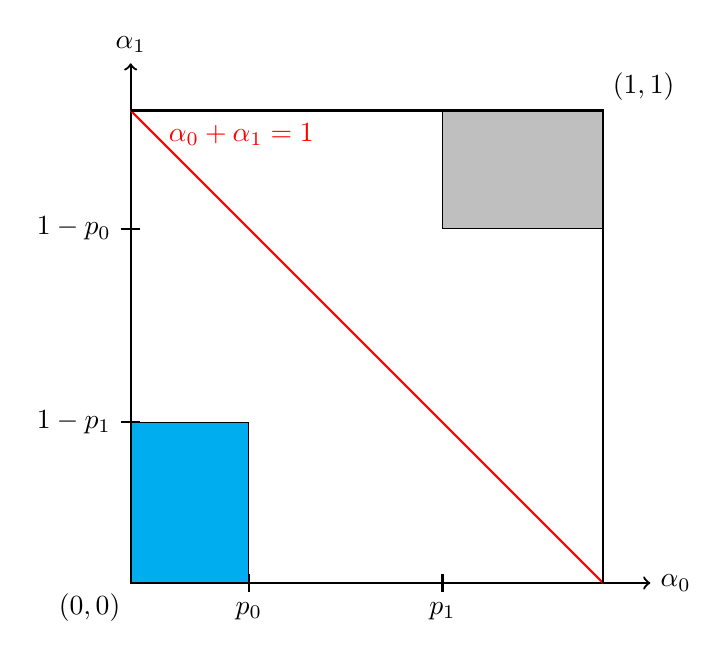
\begin{tikzpicture}[scale=6]
    \draw [fill = lightgray] (0.66,0.75) rectangle (1,1);
    \draw [fill = cyan] (0,0) rectangle (0.25, 0.34);
    \draw [thick, <->] (0,1.1)
    node[above] {$\alpha_1$} -- (0,0) 
    node [below left] {$(0,0)$} -- (1.1,0) 
    node [right] {$\alpha_0$};
    \draw [thick] (0.25,0.02) -- (0.25,-0.02) node [below] {$p_0$}; 
    \draw [thick] (0.02,0.75) -- (-0.02,0.75) node [left] {$1 - p_0$}; 
    \draw [thick] (0.66,0.02) -- (0.66,-0.02) node [below] {$p_1$}; 
    \draw [thick] (0.02,0.34) -- (-0.02,0.34) node [left] {$1 - p_1$}; 
    \draw [thick, red] (0,1) to (1,0); 
    \node [right, red] at (0.06,0.95) {$\alpha_0 + \alpha_1 = 1$};
    \draw [thick] (0,1) -- (1,1) -- (1,0);
    \node [above right] at (1,1) {$(1,1)$};
    \end{tikzpicture}
\end{figure}

\note{\singlespacing \scriptsize
  \vspace{-2.3em}
  \begin{itemize}
    \item More about assumption $\alpha_0 + \alpha_1 < 1$.
      Suppress $\mathbf{x}$. Fig.\ shows possible values of $(\alpha_0, \alpha_1)$. Red line: $\alpha_0 + \alpha_1 = 0$ so $Cor(T,T^*)=0$. Have to rule this out. Below red line $\alpha_0 + \alpha_1 <1$ so $Cor(T,T^*)>0$; above $Cor(T,T^*)<0$. Bounds on prev.\ slide assume below the red line. If we relax this, still get bounds for $\alpha_0, \alpha_1$: shaded rectangles. Blue = bounds from prev slide: $\alpha_0 \leq \min\{p_0, p_1\}$ and $\alpha_1 \leq \{1-p_0,1-p_1\}$. (In fig.\ $p_0 < p_1$). Gray means error so severe that $1-T$ is a better predictor of $T^*$ than $T$.
      So $\alpha_0 + \alpha_1 <1$ just means rule out extreme error.
      Equiv.\ to assume IV and $\beta$ have same sign.
    \item Weak bounds for $(\alpha_0, \alpha_1, \beta)$ simple and informative. Others have used related idea: Frazis \& Loewenstein (2003) and Ura (forthcoming). But weak bounds don't use non-diff assump.
      Know that non-diff is powerful: point identifies effect of an exog $T^*$.
      Can we improve upon weak bounds for endog.\ $T^*$?
    \item To answer this, derive sharp identified set under baseline assumptions: new to the literature.
      Important even if our main concern is point identification: while we showed a flaw in Mahajan's proof, we did \emph{not} show $\beta$ not point identified.
    \item How to derive sharp set? Question: for what values of unknown params can we construct valid joint dist.\ for $(y,T,T^*,z)$ compatible with observed joint for $(y,T,z)$ under our assumptions? Factorize: joint for $(T,T^*,z)$ \& conditional for $y|T,T^*,z$. Turns out that weak bounds for $(\alpha_0, \alpha_1)$ ensure valid joint for $(T,T^*,z)$ so suffices to look at conditional: $y|T,T^*,z$.
  \end{itemize}
}%
    \hyperlink{BOUNDS_BODY}{\beamergotobutton{back}}

\end{frame}
%%%%%%%%%%%%%%%%%%%%%%%%%%%%%%%%%%%%%%%%
\begin{frame}[label=IV_APPEND]
  \frametitle{What does IV estimate under mis-classification?}
  \begin{block}{Unobserved}
  \[
    \beta(\mathbf{x}) = \frac{\mathbb{E}[y|\mathbf{x},z=1] - \mathbb{E}[y|\mathbf{x},z=0]}{p^*_1(\mathbf{x}) - p^*_0(\mathbf{x})} 
  \]
  \end{block}

  \begin{block}{Wald (Observed)}
    \vspace{-1em}
    \small
    \[
      \frac{\mathbb{E}[y|\mathbf{x},z=1] - \mathbb{E}[y|\mathbf{x},z=0]}{p_1(\mathbf{x}) - p_0(\mathbf{x})} = \beta(\mathbf{x})\left[ \frac{p_1^*(\mathbf{x}) - p_0^*(\mathbf{x})}{p_1(\mathbf{x}) - p_0(\mathbf{x})} \right] = \alert{\frac{\beta(\mathbf{x})}{1 - \alpha_0(\mathbf{x}) - \alpha_1(\mathbf{x})} }
    \]
   
    \vspace{2em}
    \scriptsize
    \[
      \boxed{p_1^*(\mathbf{x}) - p_0^*(\mathbf{x}) = \frac{p_1(\mathbf{x}) - \alpha_0(\mathbf{x})}{1 - \alpha_0 - \alpha_1(\mathbf{x})} -   \frac{p_0(\mathbf{x}) - \alpha_0(\mathbf{x})}{1 - \alpha_0 - \alpha_1(\mathbf{x})} = \frac{p_1(\mathbf{x}) - p_0(\mathbf{x})}{1 - \alpha_0(\mathbf{x}) - \alpha_1(\mathbf{x})}}
    \]
  \end{block}
    \hyperlink{BOUNDS_BODY}{\beamergotobutton{back}}
\end{frame}
%%%%%%%%%%%%%%%%%%%%%%%%%%%%%%%%%%%%%%
\begin{frame}
  \frametitle{Partial Identification Bounds for $\beta(\mathbf{x})$}

    \footnotesize
    \[
      \boxed{ \beta(\mathbf{x}) = \left[ 1 - \alpha_0(\mathbf{x}) - \alpha_1(\mathbf{x}) \right] 
     \left[\frac{\mathbb{E}\left[y|\mathbf{x},z=1\right] - \mathbb{E}\left[y|\mathbf{x},z=0\right]}{p_1(\mathbf{x}) - p_0(\mathbf{x})}\right] }
    \]

    \footnotesize
    \[
      \boxed{ 0 \leq \alpha_0 \leq \min_k \{p_k(\mathbf{x})\}, \quad 0 \leq \alpha_1 \leq \min_k \{1 - p_k(\mathbf{x})\}}
    \]

    \normalsize
    \begin{block}{No Mis-classification}
      $\alpha_0(\mathbf{x}) =  \alpha_1(\mathbf{x}) = 0 \implies \alert{\beta(\mathbf{x}) = }$ \alert{Wald}
    \end{block}

    \begin{block}{Maximum Mis-classification}
      $\alpha_0(\mathbf{x}) = p_{\min}(\mathbf{x}), \, \alpha_1(\mathbf{x}) = 1 - p_{\max}(\mathbf{x})$

      \vspace{-0.5em}
      \begin{align*}
        \implies 1 - \alpha_0(\mathbf{x}) - \alpha_1(\mathbf{x}) = p_{\max}(\mathbf{x}) - p_{\min}(\mathbf{x})
      = |p_1(\mathbf{x}) - p_0(\mathbf{x})|\\
      \implies \alert{\beta(\mathbf{x}) =\mbox{sign}\left\{ p_1(\mathbf{x}) - p_0(\mathbf{x}) \right\}\times (\mbox{Reduced Form})}
    \end{align*}
      
    \end{block}
  
    \hyperlink{BOUNDS_BODY}{\beamergotobutton{back}}
\end{frame}
%%%%%%%%%%%%%%%%%%%%%%%%%%%%%%%%%%%%%%
\begin{frame}[label=MEQS_APPEND]
  \frametitle{Just-Identified System of Moment Equalities}
  \framesubtitle{Suppress dependence on $\mathbf{x}$\dots} 

  \small
\[
\mathbb{E}\left[
  \left\{\boldsymbol{\Psi}(\boldsymbol{\theta})\mathbf{w}_i - \boldsymbol{\kappa}\right\} \otimes 
\left(
\begin{array}{c}
  1 \\ z
\end{array}\right)
\right] = \mathbf{0}
\]

  \footnotesize
\[
  \boldsymbol{\Psi}(\boldsymbol{\theta}) \equiv
 \left[
  \begin{array}{rrrrrr}
    -\theta_1 & 1 & 0 & 0 & 0 & 0\\
    \theta_2 & 0 & -2\theta_1 & 1 & 0 & 0\\ 
    -\theta_3 & 0 & 3\theta_2 & 0 & -3\theta_1 & 1
\end{array}\right]
\]

  \begin{align*}
\mathbf{w}_i &= (T_i, y_i, y_iT_i, y_i^2, y_i^2 T_i, y_i^3)' &
  \theta_1 &= \beta/(1 - \alpha_0 - \alpha_1) \\
\boldsymbol{\kappa} &= (\kappa_1, \kappa_2, \kappa_3)'  &
  \theta_2 &= \theta_1^2 (1 + \alpha_0 - \alpha_1)\\
  & & \theta_3 &= \theta_1^3\left[ (1 - \alpha_0 - \alpha_1)^2 + 6\alpha_0(1 - \alpha_1) \right] 
\end{align*}

    \hyperlink{INEQ_BODY}{\beamergotobutton{back}}
\end{frame}
%%%%%%%%%%%%%%%%%%%%%%%%%%%%%%%%%%%%%
\begin{frame}[label=INEQ_APPEND]
  \frametitle{Moment Inequalities I -- First-stage Probabilities}

  $\alpha_0 \leq p_k \leq 1 - \alpha_1$ becomes $\alert{\mathbb{E}\left[ m(\mathbf{w}_i,\boldsymbol{\vartheta} ) \right] \geq \mathbf{0}}$ for all $k$ where
\[
  m(\mathbf{w}_i, \boldsymbol{\vartheta}) \equiv \left[
  \begin{array}{l}
    \mathbf{1}(z_i=k)(T - \alpha_0) \\
    \mathbf{1}(z_i = k) (1 - T_i - \alpha_1) 
  \end{array}
\right]
\]
  
\end{frame}

%%%%%%%%%%%%%%%%%%%%%%%%%%%%%%%%%%%%%
\begin{frame}
  \frametitle{Moment Inequalities II -- Non-differential Assumption}

  \scriptsize

  For all $k$, we have $\alert{\mathbb{E}[m\big(\mathbf{w}_i, \boldsymbol{\vartheta}, \mathbf{q}_k)]\geq 0}$ where
\[
  m\big(\mathbf{w}_i, \boldsymbol{\vartheta}, \mathbf{q}_k) \equiv \left[
  \begin{array}{r}
    y_i \mathbf{1}\left( z_i=k \right)\left\{(T_i - \alpha_0) - \mathbf{1}(y_i \leq \underline{q}_{0k})  (1 - T_i)\left( \frac{1 - \alpha_0 - \alpha_1}{\alpha_1} \right)\right\} \\
    - y_i \mathbf{1}(z_i=k) \left\{ (T_i - \alpha_0) -  \mathbf{1}(y_i > \overline{q}_{0k}) (1 - T_i) \left( \frac{1 - \alpha_0 - \alpha_1}{\alpha_1} \right) \right\} \\
    y_i \mathbf{1}\left( z_i=k \right)\left\{(T_i - \alpha_0) - \mathbf{1}(y_i \leq \underline{q}_{1k})  T_i\left( \frac{1 - \alpha_0 - \alpha_1}{1 - \alpha_1} \right)\right\} \\
    - y_i \mathbf{1}(z_i=k) \left\{ (T_i - \alpha_0) -  \mathbf{1}(y_i > \overline{q}_{1k}) T_i \left( \frac{1 - \alpha_0 - \alpha_1}{1 - \alpha_1} \right) \right\} 
\end{array}
\right] 
\]
and $\alert{\mathbf{q}_k \equiv ( \underline{q}_{0k},\, \overline{q}_{0k},\, \underline{q}_{1k}, \,\overline{q}_{1k})'}$ defined by $\alert{\mathbb{E}[h(\mathbf{w}_i,\boldsymbol{\vartheta},\mathbf{q}_k)]=0}$ with
\[
  h(\mathbf{w}_i,\boldsymbol{\vartheta},\mathbf{q}_k) = \left[
  \begin{array}{l}
    \mathbf{1}(y_i \leq \underline{q}_{0k}) \mathbf{1}(z_i=k)(1 - T_i) 
    - \left( \frac{\alpha_1}{1 - \alpha_0 - \alpha_1} \right) \mathbf{1}(z_i=k)(T_i-\alpha_0)\\ 
    \mathbf{1}(y_i \leq \overline{q}_{0k}) \mathbf{1}(z_i=k)(1 - T_i)
    - \left( \frac{1 - \alpha_0}{1 - \alpha_0 - \alpha_1} \right) \mathbf{1}(z_i=k)(1 - T_i-\alpha_1)\\
    \mathbf{1}(y_i \leq \underline{q}_{1k}) \mathbf{1}(z_i=k)T_i
    - \left( \frac{1 - \alpha_1}{1 - \alpha_0 - \alpha_1} \right) \mathbf{1}(z_i=k)(T_i-\alpha_0)\\ 
    \mathbf{1}(y_i \leq \overline{q}_{1k}) \mathbf{1}(z_i=k)T_i 
    - \left( \frac{\alpha_0}{1 - \alpha_0 - \alpha_1} \right) \mathbf{1}(z_i=k)(1 - T_i-\alpha_1)
  \end{array}
\right]
\]

    \hyperlink{INEQ_BODY}{\beamergotobutton{back}}
\end{frame}
%%%%%%%%%%%%%%%%%%%%%%%%%%%%%%%%%%%%%
\end{document}
